% Options for packages loaded elsewhere
\PassOptionsToPackage{unicode}{hyperref}
\PassOptionsToPackage{hyphens}{url}
%
\documentclass[
]{article}
\usepackage{lmodern}
\usepackage{amssymb,amsmath}
\usepackage{ifxetex,ifluatex}
\ifnum 0\ifxetex 1\fi\ifluatex 1\fi=0 % if pdftex
  \usepackage[T1]{fontenc}
  \usepackage[utf8]{inputenc}
  \usepackage{textcomp} % provide euro and other symbols
\else % if luatex or xetex
  \usepackage{unicode-math}
  \defaultfontfeatures{Scale=MatchLowercase}
  \defaultfontfeatures[\rmfamily]{Ligatures=TeX,Scale=1}
\fi
% Use upquote if available, for straight quotes in verbatim environments
\IfFileExists{upquote.sty}{\usepackage{upquote}}{}
\IfFileExists{microtype.sty}{% use microtype if available
  \usepackage[]{microtype}
  \UseMicrotypeSet[protrusion]{basicmath} % disable protrusion for tt fonts
}{}
\makeatletter
\@ifundefined{KOMAClassName}{% if non-KOMA class
  \IfFileExists{parskip.sty}{%
    \usepackage{parskip}
  }{% else
    \setlength{\parindent}{0pt}
    \setlength{\parskip}{6pt plus 2pt minus 1pt}}
}{% if KOMA class
  \KOMAoptions{parskip=half}}
\makeatother
\usepackage{xcolor}
\IfFileExists{xurl.sty}{\usepackage{xurl}}{} % add URL line breaks if available
\IfFileExists{bookmark.sty}{\usepackage{bookmark}}{\usepackage{hyperref}}
\hypersetup{
  pdftitle={Dropout Prediction: A Systematic Literature Review},
  hidelinks,
  pdfcreator={LaTeX via pandoc}}
\urlstyle{same} % disable monospaced font for URLs
\usepackage[margin=1in]{geometry}
\usepackage{color}
\usepackage{fancyvrb}
\newcommand{\VerbBar}{|}
\newcommand{\VERB}{\Verb[commandchars=\\\{\}]}
\DefineVerbatimEnvironment{Highlighting}{Verbatim}{commandchars=\\\{\}}
% Add ',fontsize=\small' for more characters per line
\usepackage{framed}
\definecolor{shadecolor}{RGB}{248,248,248}
\newenvironment{Shaded}{\begin{snugshade}}{\end{snugshade}}
\newcommand{\AlertTok}[1]{\textcolor[rgb]{0.94,0.16,0.16}{#1}}
\newcommand{\AnnotationTok}[1]{\textcolor[rgb]{0.56,0.35,0.01}{\textbf{\textit{#1}}}}
\newcommand{\AttributeTok}[1]{\textcolor[rgb]{0.77,0.63,0.00}{#1}}
\newcommand{\BaseNTok}[1]{\textcolor[rgb]{0.00,0.00,0.81}{#1}}
\newcommand{\BuiltInTok}[1]{#1}
\newcommand{\CharTok}[1]{\textcolor[rgb]{0.31,0.60,0.02}{#1}}
\newcommand{\CommentTok}[1]{\textcolor[rgb]{0.56,0.35,0.01}{\textit{#1}}}
\newcommand{\CommentVarTok}[1]{\textcolor[rgb]{0.56,0.35,0.01}{\textbf{\textit{#1}}}}
\newcommand{\ConstantTok}[1]{\textcolor[rgb]{0.00,0.00,0.00}{#1}}
\newcommand{\ControlFlowTok}[1]{\textcolor[rgb]{0.13,0.29,0.53}{\textbf{#1}}}
\newcommand{\DataTypeTok}[1]{\textcolor[rgb]{0.13,0.29,0.53}{#1}}
\newcommand{\DecValTok}[1]{\textcolor[rgb]{0.00,0.00,0.81}{#1}}
\newcommand{\DocumentationTok}[1]{\textcolor[rgb]{0.56,0.35,0.01}{\textbf{\textit{#1}}}}
\newcommand{\ErrorTok}[1]{\textcolor[rgb]{0.64,0.00,0.00}{\textbf{#1}}}
\newcommand{\ExtensionTok}[1]{#1}
\newcommand{\FloatTok}[1]{\textcolor[rgb]{0.00,0.00,0.81}{#1}}
\newcommand{\FunctionTok}[1]{\textcolor[rgb]{0.00,0.00,0.00}{#1}}
\newcommand{\ImportTok}[1]{#1}
\newcommand{\InformationTok}[1]{\textcolor[rgb]{0.56,0.35,0.01}{\textbf{\textit{#1}}}}
\newcommand{\KeywordTok}[1]{\textcolor[rgb]{0.13,0.29,0.53}{\textbf{#1}}}
\newcommand{\NormalTok}[1]{#1}
\newcommand{\OperatorTok}[1]{\textcolor[rgb]{0.81,0.36,0.00}{\textbf{#1}}}
\newcommand{\OtherTok}[1]{\textcolor[rgb]{0.56,0.35,0.01}{#1}}
\newcommand{\PreprocessorTok}[1]{\textcolor[rgb]{0.56,0.35,0.01}{\textit{#1}}}
\newcommand{\RegionMarkerTok}[1]{#1}
\newcommand{\SpecialCharTok}[1]{\textcolor[rgb]{0.00,0.00,0.00}{#1}}
\newcommand{\SpecialStringTok}[1]{\textcolor[rgb]{0.31,0.60,0.02}{#1}}
\newcommand{\StringTok}[1]{\textcolor[rgb]{0.31,0.60,0.02}{#1}}
\newcommand{\VariableTok}[1]{\textcolor[rgb]{0.00,0.00,0.00}{#1}}
\newcommand{\VerbatimStringTok}[1]{\textcolor[rgb]{0.31,0.60,0.02}{#1}}
\newcommand{\WarningTok}[1]{\textcolor[rgb]{0.56,0.35,0.01}{\textbf{\textit{#1}}}}
\usepackage{graphicx}
\makeatletter
\def\maxwidth{\ifdim\Gin@nat@width>\linewidth\linewidth\else\Gin@nat@width\fi}
\def\maxheight{\ifdim\Gin@nat@height>\textheight\textheight\else\Gin@nat@height\fi}
\makeatother
% Scale images if necessary, so that they will not overflow the page
% margins by default, and it is still possible to overwrite the defaults
% using explicit options in \includegraphics[width, height, ...]{}
\setkeys{Gin}{width=\maxwidth,height=\maxheight,keepaspectratio}
% Set default figure placement to htbp
\makeatletter
\def\fps@figure{htbp}
\makeatother
\setlength{\emergencystretch}{3em} % prevent overfull lines
\providecommand{\tightlist}{%
  \setlength{\itemsep}{0pt}\setlength{\parskip}{0pt}}
\setcounter{secnumdepth}{-\maxdimen} % remove section numbering

\title{Dropout Prediction: A Systematic Literature Review}
\author{}
\date{\vspace{-2.5em}}

\begin{document}
\maketitle

This is an \href{http://rmarkdown.rstudio.com}{R Markdown} Notebook.
With the cleaning of a dataframe used in a Systematic Review.
\url{https://cran.r-project.org/web/packages/bibtex/bibtex.pdf}

This was tested with bib2df version 1.1.1, installation instructions
available \href{https://docs.ropensci.org/bib2df/}{here}, and one
example
\href{https://docs.ropensci.org/bib2df/articles/bib2df.html}{here}.
Github project is available
\href{https://github.com/ropensci/bib2df}{here}

Is better to confirm that the files are in UTF-8 encoding. The bibtex
files must be checked. There should be spaces between ``='':

\begin{verbatim}
@Article{Binmore2008,
  Title = {Do Conventions Need to Be Common Knowledge?},
  Author = {Binmore, Ken},
  Journal = {Topoi},
  Year = {2008},
  Number = {1},
  Pages = {17--27},
  Volume = {27}
}
\end{verbatim}

This code correct that:

\begin{verbatim}
tx<-readLines(file)
tx2<-gsub(pattern = "=\\{",replacement = " = {",x = tx)
writeLines(text = tx2,con = 'corrected_scopus.bib')
\end{verbatim}

\hypertarget{import-libraries}{%
\section{Import Libraries}\label{import-libraries}}

\begin{Shaded}
\begin{Highlighting}[]
\CommentTok{\# Setup library}
\KeywordTok{library}\NormalTok{(bib2df)}
\KeywordTok{library}\NormalTok{(bibtex)}
\KeywordTok{library}\NormalTok{(tibble)}
\KeywordTok{library}\NormalTok{(dplyr)}

\KeywordTok{setwd}\NormalTok{(}\StringTok{\textquotesingle{}C:/nuvem/Dropbox/doutoramento/tese/SLRDropout/analysis\textquotesingle{}}\NormalTok{)}
\end{Highlighting}
\end{Shaded}

List all the files with bib extension

\begin{Shaded}
\begin{Highlighting}[]
\NormalTok{files\textless{}{-}}\KeywordTok{list.files}\NormalTok{(}\DataTypeTok{path =} \StringTok{\textquotesingle{}articles/\textquotesingle{}}\NormalTok{,}\DataTypeTok{pattern =} \StringTok{\textquotesingle{}}\CharTok{\textbackslash{}\textbackslash{}}\StringTok{.bib$\textquotesingle{}}\NormalTok{)}
\NormalTok{files}
\end{Highlighting}
\end{Shaded}

\begin{verbatim}
##  [1] "acm.bib"                               
##  [2] "ieee.bib"                              
##  [3] "parsifal_data_articles.bib"            
##  [4] "scienceDirect_withContractual1.bib"    
##  [5] "scienceDirect_withContractual2.bib"    
##  [6] "scopus._test.bib"                      
##  [7] "scopus.bib"                            
##  [8] "scopus_zotero.bib"                     
##  [9] "springer_Exported Items.bib"           
## [10] "tempieee.bib"                          
## [11] "tempscienceDirect_withContractual1.bib"
## [12] "tempscienceDirect_withContractual2.bib"
## [13] "tempscopus_zotero.bib"                 
## [14] "webofscience_Exported Items.bib"
\end{verbatim}

Reading bibtex source files

\hypertarget{acm}{%
\section{ACM}\label{acm}}

\begin{Shaded}
\begin{Highlighting}[]
\NormalTok{acm\textless{}{-}}\KeywordTok{bib2df}\NormalTok{(}\DataTypeTok{file =} \StringTok{\textquotesingle{}articles/acm.bib\textquotesingle{}}\NormalTok{)}
\CommentTok{\#str(acm)}
\NormalTok{acm2\textless{}{-}}\KeywordTok{read.bib}\NormalTok{(}\DataTypeTok{file =} \StringTok{\textquotesingle{}articles/acm.bib\textquotesingle{}}\NormalTok{,}\DataTypeTok{encoding =} \StringTok{\textquotesingle{}UTF8\textquotesingle{}}\NormalTok{)}
\KeywordTok{str}\NormalTok{(acm)}
\end{Highlighting}
\end{Shaded}

\begin{verbatim}
## tibble [8 x 36] (S3: tbl_df/tbl/data.frame)
##  $ CATEGORY    : chr [1:8] "INPROCEEDINGS" "INPROCEEDINGS" "INPROCEEDINGS" "ARTICLE" ...
##  $ BIBTEXKEY   : chr [1:8] "10.1145/3195106.3195178" "10.1145/3009977.3010073" "10.1145/2808797.2808821" "10.1145/2594473.2594475" ...
##  $ ADDRESS     : chr [1:8] "New York, NY, USA" "New York, NY, USA" "New York, NY, USA" "New York, NY, USA" ...
##  $ ANNOTE      : chr [1:8] NA NA NA NA ...
##  $ AUTHOR      :List of 8
##   ..$ : chr [1:2] "Cui, Shaoying" "Ding, Ning"
##   ..$ : chr [1:2] "I, Shahid K" "Chaudhury, Santanu"
##   ..$ : chr [1:3] "G\\\"{o}k, Mehmet" "\\\"{O}zyer, Tansel" "Jida, Jamal"
##   ..$ : chr "Freitas, Alex A."
##   ..$ : chr [1:2] "Gupta, Gunjan" "Ghosh, Joydeep"
##   ..$ : chr [1:4] "Zimbra, David" "Abbasi, Ahmed" "Zeng, Daniel" "Chen, Hsinchun"
##   ..$ : chr NA
##   ..$ : chr [1:5] "Nagano, Shouichi" "Ichikawa, Yusuke" "Takaya, Noriko" "Uchiyama, Tadasu" ...
##  $ BOOKTITLE   : chr [1:8] "Proceedings of the 2018 10th International Conference on Machine Learning and Computing" "Proceedings of the Tenth Indian Conference on Computer Vision, Graphics and Image Processing" "Proceedings of the 2015 IEEE/ACM International Conference on Advances in Social Networks Analysis and Mining 2015" NA ...
##  $ CHAPTER     : chr [1:8] NA NA NA NA ...
##  $ CROSSREF    : chr [1:8] NA NA NA NA ...
##  $ EDITION     : chr [1:8] NA NA NA NA ...
##  $ EDITOR      :List of 8
##   ..$ : chr NA
##   ..$ : chr NA
##   ..$ : chr NA
##   ..$ : chr NA
##   ..$ : chr NA
##   ..$ : chr NA
##   ..$ : chr NA
##   ..$ : chr NA
##  $ HOWPUBLISHED: chr [1:8] NA NA NA NA ...
##  $ INSTITUTION : chr [1:8] NA NA NA NA ...
##  $ JOURNAL     : chr [1:8] NA NA NA "SIGKDD Explor. Newsl." ...
##  $ KEY         : chr [1:8] NA NA NA NA ...
##  $ MONTH       : chr [1:8] NA NA NA "mar" ...
##  $ NOTE        : chr [1:8] NA NA NA NA ...
##  $ NUMBER      : chr [1:8] NA NA NA "1" ...
##  $ ORGANIZATION: chr [1:8] NA NA NA NA ...
##  $ PAGES       : chr [1:8] "161â\200“166" NA "1220â\200“1224" "1â\200“10" ...
##  $ PUBLISHER   : chr [1:8] "Association for Computing Machinery" "Association for Computing Machinery" "Association for Computing Machinery" "Association for Computing Machinery" ...
##  $ SCHOOL      : chr [1:8] NA NA NA NA ...
##  $ SERIES      : chr [1:8] "ICMLC 2018" "ICVGIP '16" "ASONAM '15" NA ...
##  $ TITLE       : chr [1:8] "Construction of a Bank Customer Data Warehouse and an Application of Data Mining" "Scalable Clustering and Applications" "A Case Study for the Churn Prediction in Turksat Internet Service Subscription" "Comprehensible Classification Models: A Position Paper" ...
##  $ TYPE        : chr [1:8] NA NA NA NA ...
##  $ VOLUME      : chr [1:8] NA NA NA "15" ...
##  $ YEAR        : num [1:8] 2018 2016 2015 2014 2008 ...
##  $ ISBN        : chr [1:8] "9781450363532" "9781450347532" "9781450338547" NA ...
##  $ URL         : chr [1:8] "https://doi.org/10.1145/3195106.3195178" "https://doi.org/10.1145/3009977.3010073" "https://doi.org/10.1145/2808797.2808821" "https://doi.org/10.1145/2594473.2594475" ...
##  $ DOI         : chr [1:8] "10.1145/3195106.3195178" "10.1145/3009977.3010073" "10.1145/2808797.2808821" "10.1145/2594473.2594475" ...
##  $ ABSTRACT    : chr [1:8] "In this era of strong competition, data mining can provide effective support to bank operators in their effort "| __truncated__ "Large scale machine learning is becoming an active research area recently. Most of the existing clustering algo"| __truncated__ "Churn prediction is a customer relationship process that predicts for customers who are at the brink of transfe"| __truncated__ "The vast majority of the literature evaluates the performance of classification models using only the criterion"| __truncated__ ...
##  $ NUMPAGES    : chr [1:8] "6" "7" "5" "10" ...
##  $ KEYWORDS    : chr [1:8] "Bank customer information, data mining, data warehouse, multidimensional data analysis" "large scale machine learning, segmentation and grouping" "Customer relationship management, data mining, time series clustering, hierarchical clustering, recursive parti"| __truncated__ "decision tree, monotonicity constraint, nearest neighbors, Bayesian network classifiers, decision table, rule induction" ...
##  $ LOCATION    : chr [1:8] "Macau, China" "Guwahati, Assam, India" "Paris, France" NA ...
##  $ ARTICLENO   : chr [1:8] NA "34" NA NA ...
##  $ ISSUE_DATE  : chr [1:8] NA NA NA "June 2013" ...
##  $ ISSN        : chr [1:8] NA NA NA "1931-0145" ...
\end{verbatim}

\begin{Shaded}
\begin{Highlighting}[]
\KeywordTok{names}\NormalTok{(acm)}
\end{Highlighting}
\end{Shaded}

\begin{verbatim}
##  [1] "CATEGORY"     "BIBTEXKEY"    "ADDRESS"      "ANNOTE"       "AUTHOR"      
##  [6] "BOOKTITLE"    "CHAPTER"      "CROSSREF"     "EDITION"      "EDITOR"      
## [11] "HOWPUBLISHED" "INSTITUTION"  "JOURNAL"      "KEY"          "MONTH"       
## [16] "NOTE"         "NUMBER"       "ORGANIZATION" "PAGES"        "PUBLISHER"   
## [21] "SCHOOL"       "SERIES"       "TITLE"        "TYPE"         "VOLUME"      
## [26] "YEAR"         "ISBN"         "URL"          "DOI"          "ABSTRACT"    
## [31] "NUMPAGES"     "KEYWORDS"     "LOCATION"     "ARTICLENO"    "ISSUE_DATE"  
## [36] "ISSN"
\end{verbatim}

\begin{Shaded}
\begin{Highlighting}[]
\CommentTok{\#Exclude some columns not required for the analysis}
\NormalTok{acm \textless{}{-}}\StringTok{ }\NormalTok{acm }\OperatorTok{\%\textgreater{}\%}\StringTok{ }\KeywordTok{select}\NormalTok{(}\OperatorTok{{-}}\KeywordTok{c}\NormalTok{(CHAPTER}\OperatorTok{:}\NormalTok{INSTITUTION,KEY}\OperatorTok{:}\NormalTok{ORGANIZATION,ANNOTE,SCHOOL,TYPE,ISSUE\_DATE))}
\KeywordTok{str}\NormalTok{(acm)}
\end{Highlighting}
\end{Shaded}

\begin{verbatim}
## tibble [8 x 21] (S3: tbl_df/tbl/data.frame)
##  $ CATEGORY : chr [1:8] "INPROCEEDINGS" "INPROCEEDINGS" "INPROCEEDINGS" "ARTICLE" ...
##  $ BIBTEXKEY: chr [1:8] "10.1145/3195106.3195178" "10.1145/3009977.3010073" "10.1145/2808797.2808821" "10.1145/2594473.2594475" ...
##  $ ADDRESS  : chr [1:8] "New York, NY, USA" "New York, NY, USA" "New York, NY, USA" "New York, NY, USA" ...
##  $ AUTHOR   :List of 8
##   ..$ : chr [1:2] "Cui, Shaoying" "Ding, Ning"
##   ..$ : chr [1:2] "I, Shahid K" "Chaudhury, Santanu"
##   ..$ : chr [1:3] "G\\\"{o}k, Mehmet" "\\\"{O}zyer, Tansel" "Jida, Jamal"
##   ..$ : chr "Freitas, Alex A."
##   ..$ : chr [1:2] "Gupta, Gunjan" "Ghosh, Joydeep"
##   ..$ : chr [1:4] "Zimbra, David" "Abbasi, Ahmed" "Zeng, Daniel" "Chen, Hsinchun"
##   ..$ : chr NA
##   ..$ : chr [1:5] "Nagano, Shouichi" "Ichikawa, Yusuke" "Takaya, Noriko" "Uchiyama, Tadasu" ...
##  $ BOOKTITLE: chr [1:8] "Proceedings of the 2018 10th International Conference on Machine Learning and Computing" "Proceedings of the Tenth Indian Conference on Computer Vision, Graphics and Image Processing" "Proceedings of the 2015 IEEE/ACM International Conference on Advances in Social Networks Analysis and Mining 2015" NA ...
##  $ JOURNAL  : chr [1:8] NA NA NA "SIGKDD Explor. Newsl." ...
##  $ PAGES    : chr [1:8] "161â\200“166" NA "1220â\200“1224" "1â\200“10" ...
##  $ PUBLISHER: chr [1:8] "Association for Computing Machinery" "Association for Computing Machinery" "Association for Computing Machinery" "Association for Computing Machinery" ...
##  $ SERIES   : chr [1:8] "ICMLC 2018" "ICVGIP '16" "ASONAM '15" NA ...
##  $ TITLE    : chr [1:8] "Construction of a Bank Customer Data Warehouse and an Application of Data Mining" "Scalable Clustering and Applications" "A Case Study for the Churn Prediction in Turksat Internet Service Subscription" "Comprehensible Classification Models: A Position Paper" ...
##  $ VOLUME   : chr [1:8] NA NA NA "15" ...
##  $ YEAR     : num [1:8] 2018 2016 2015 2014 2008 ...
##  $ ISBN     : chr [1:8] "9781450363532" "9781450347532" "9781450338547" NA ...
##  $ URL      : chr [1:8] "https://doi.org/10.1145/3195106.3195178" "https://doi.org/10.1145/3009977.3010073" "https://doi.org/10.1145/2808797.2808821" "https://doi.org/10.1145/2594473.2594475" ...
##  $ DOI      : chr [1:8] "10.1145/3195106.3195178" "10.1145/3009977.3010073" "10.1145/2808797.2808821" "10.1145/2594473.2594475" ...
##  $ ABSTRACT : chr [1:8] "In this era of strong competition, data mining can provide effective support to bank operators in their effort "| __truncated__ "Large scale machine learning is becoming an active research area recently. Most of the existing clustering algo"| __truncated__ "Churn prediction is a customer relationship process that predicts for customers who are at the brink of transfe"| __truncated__ "The vast majority of the literature evaluates the performance of classification models using only the criterion"| __truncated__ ...
##  $ NUMPAGES : chr [1:8] "6" "7" "5" "10" ...
##  $ KEYWORDS : chr [1:8] "Bank customer information, data mining, data warehouse, multidimensional data analysis" "large scale machine learning, segmentation and grouping" "Customer relationship management, data mining, time series clustering, hierarchical clustering, recursive parti"| __truncated__ "decision tree, monotonicity constraint, nearest neighbors, Bayesian network classifiers, decision table, rule induction" ...
##  $ LOCATION : chr [1:8] "Macau, China" "Guwahati, Assam, India" "Paris, France" NA ...
##  $ ARTICLENO: chr [1:8] NA "34" NA NA ...
##  $ ISSN     : chr [1:8] NA NA NA "1931-0145" ...
\end{verbatim}

\hypertarget{ieee}{%
\section{IEEE}\label{ieee}}

\begin{Shaded}
\begin{Highlighting}[]
\NormalTok{ieee\textless{}{-}}\KeywordTok{bib2df}\NormalTok{(}\DataTypeTok{file =} \StringTok{\textquotesingle{}articles/ieee.bib\textquotesingle{}}\NormalTok{)}
\KeywordTok{names}\NormalTok{(ieee)}
\end{Highlighting}
\end{Shaded}

\begin{verbatim}
##  [1] "CATEGORY"     "BIBTEXKEY"    "ADDRESS"      "ANNOTE"       "AUTHOR"      
##  [6] "BOOKTITLE"    "CHAPTER"      "CROSSREF"     "EDITION"      "EDITOR"      
## [11] "HOWPUBLISHED" "INSTITUTION"  "JOURNAL"      "KEY"          "MONTH"       
## [16] "NOTE"         "NUMBER"       "ORGANIZATION" "PAGES"        "PUBLISHER"   
## [21] "SCHOOL"       "SERIES"       "TITLE"        "TYPE"         "VOLUME"      
## [26] "YEAR"         "ABSTRACT"     "KEYWORDS"     "DOI"          "ISSN"
\end{verbatim}

\begin{Shaded}
\begin{Highlighting}[]
\KeywordTok{dim}\NormalTok{(ieee)}
\end{Highlighting}
\end{Shaded}

\begin{verbatim}
## [1] 20 30
\end{verbatim}

\hypertarget{science-direct}{%
\section{Science Direct}\label{science-direct}}

\begin{Shaded}
\begin{Highlighting}[]
\NormalTok{science1\textless{}{-}}\KeywordTok{bib2df}\NormalTok{(}\DataTypeTok{file =} \StringTok{\textquotesingle{}articles/scienceDirect\_withContractual1.bib\textquotesingle{}}\NormalTok{)}
\KeywordTok{dim}\NormalTok{(science1)}
\end{Highlighting}
\end{Shaded}

\begin{verbatim}
## [1] 100  34
\end{verbatim}

\begin{Shaded}
\begin{Highlighting}[]
\NormalTok{science2\textless{}{-}}\KeywordTok{bib2df}\NormalTok{(}\DataTypeTok{file =} \StringTok{\textquotesingle{}articles/scienceDirect\_withContractual2.bib\textquotesingle{}}\NormalTok{)}
\KeywordTok{dim}\NormalTok{(science2)}
\end{Highlighting}
\end{Shaded}

\begin{verbatim}
## [1] 26 34
\end{verbatim}

\begin{Shaded}
\begin{Highlighting}[]
\CommentTok{\#merge two dataframes}
\NormalTok{science \textless{}{-}}\StringTok{ }\KeywordTok{rbind}\NormalTok{(science1,science2)}
\KeywordTok{dim}\NormalTok{(science)}
\end{Highlighting}
\end{Shaded}

\begin{verbatim}
## [1] 126  34
\end{verbatim}

\begin{Shaded}
\begin{Highlighting}[]
\KeywordTok{names}\NormalTok{(science)}
\end{Highlighting}
\end{Shaded}

\begin{verbatim}
##  [1] "CATEGORY"     "BIBTEXKEY"    "ADDRESS"      "ANNOTE"       "AUTHOR"      
##  [6] "BOOKTITLE"    "CHAPTER"      "CROSSREF"     "EDITION"      "EDITOR"      
## [11] "HOWPUBLISHED" "INSTITUTION"  "JOURNAL"      "KEY"          "MONTH"       
## [16] "NOTE"         "NUMBER"       "ORGANIZATION" "PAGES"        "PUBLISHER"   
## [21] "SCHOOL"       "SERIES"       "TITLE"        "TYPE"         "VOLUME"      
## [26] "YEAR"         "ISSN"         "DOI"          "URL"          "KEYWORDS"    
## [31] "ABSTRACT"     "ISBN"         "SHORTTITLE"   "LANGUAGE"
\end{verbatim}

\begin{Shaded}
\begin{Highlighting}[]
\KeywordTok{ls}\NormalTok{() }\CommentTok{\# check object in workspace}
\end{Highlighting}
\end{Shaded}

\begin{verbatim}
## [1] "acm"      "acm2"     "files"    "ieee"     "science"  "science1" "science2"
\end{verbatim}

\begin{Shaded}
\begin{Highlighting}[]
\CommentTok{\#remove dataframes}
\KeywordTok{rm}\NormalTok{(science1)}
\KeywordTok{rm}\NormalTok{(science2)}
\end{Highlighting}
\end{Shaded}

Incorrect data discarded 8 incomplete information tot

\begin{Shaded}
\begin{Highlighting}[]
\KeywordTok{dim}\NormalTok{(science)}
\end{Highlighting}
\end{Shaded}

\begin{verbatim}
## [1] 126  34
\end{verbatim}

\begin{Shaded}
\begin{Highlighting}[]
\KeywordTok{length}\NormalTok{(}\KeywordTok{unique}\NormalTok{(science}\OperatorTok{$}\NormalTok{ABSTRACT))}
\end{Highlighting}
\end{Shaded}

\begin{verbatim}
## [1] 118
\end{verbatim}

There are 6 entries without abstract.

\begin{Shaded}
\begin{Highlighting}[]
\NormalTok{science\_Abstract \textless{}{-}}\StringTok{ }\NormalTok{science }\OperatorTok{\%\textgreater{}\%}\StringTok{ }\KeywordTok{filter}\NormalTok{(}\KeywordTok{is.na}\NormalTok{(ABSTRACT)) }\OperatorTok{\%\textgreater{}\%}\StringTok{ }\KeywordTok{select}\NormalTok{(TITLE,ABSTRACT,URL,DOI)}
\KeywordTok{str}\NormalTok{(science\_Abstract)}
\end{Highlighting}
\end{Shaded}

\begin{verbatim}
## tibble [9 x 4] (S3: tbl_df/tbl/data.frame)
##  $ TITLE   : chr [1:9] "Index" "Abstracts" "Abstracts" "Abstracts" ...
##  $ ABSTRACT: chr [1:9] NA NA NA NA ...
##  $ URL     : chr [1:9] "http://www.sciencedirect.com/science/article/pii/B9780128042915000271" "http://www.sciencedirect.com/science/article/pii/S0140670120300266" "http://www.sciencedirect.com/science/article/pii/S0140670113000039" "http://www.sciencedirect.com/science/article/pii/S0140670120300187" ...
##  $ DOI     : chr [1:9] "https://doi.org/10.1016/B978-0-12-804291-5.00027-1" "https://doi.org/10.1016/j.fueleneab.2020.07.002" "https://doi.org/10.1016/j.fueleneab.2013.01.002" "https://doi.org/10.1016/j.fueleneab.2020.05.002" ...
\end{verbatim}

\begin{Shaded}
\begin{Highlighting}[]
\KeywordTok{unique}\NormalTok{(science\_Abstract}\OperatorTok{$}\NormalTok{TITLE)}
\end{Highlighting}
\end{Shaded}

\begin{verbatim}
## [1] "Index"                             "Abstracts"                        
## [3] "Front cover and table of contents" "Technical Program"                
## [5] "Subject Index"                     "Contents"
\end{verbatim}

\begin{Shaded}
\begin{Highlighting}[]
\NormalTok{science\_Abstract}\OperatorTok{$}\NormalTok{TITLE}
\end{Highlighting}
\end{Shaded}

\begin{verbatim}
## [1] "Index"                             "Abstracts"                        
## [3] "Abstracts"                         "Abstracts"                        
## [5] "Front cover and table of contents" "Technical Program"                
## [7] "Subject Index"                     "Contents"                         
## [9] "Abstracts"
\end{verbatim}

The entries aren't articles, we will remove them.

\begin{Shaded}
\begin{Highlighting}[]
\NormalTok{science\_correct \textless{}{-}}\StringTok{ }\NormalTok{science }\OperatorTok{\%\textgreater{}\%}\StringTok{ }\KeywordTok{filter}\NormalTok{(}\OperatorTok{!}\KeywordTok{is.na}\NormalTok{(ABSTRACT)) }
\end{Highlighting}
\end{Shaded}

\hypertarget{scopus}{%
\section{Scopus}\label{scopus}}

\begin{Shaded}
\begin{Highlighting}[]
\NormalTok{scopus \textless{}{-}}\StringTok{ }\KeywordTok{bib2df}\NormalTok{(}\StringTok{\textquotesingle{}articles/scopus.bib\textquotesingle{}}\NormalTok{)}
\KeywordTok{dim}\NormalTok{(scopus)}
\end{Highlighting}
\end{Shaded}

\begin{verbatim}
## [1] 210  32
\end{verbatim}

\begin{Shaded}
\begin{Highlighting}[]
\KeywordTok{names}\NormalTok{(scopus)}
\end{Highlighting}
\end{Shaded}

\begin{verbatim}
##  [1] "CATEGORY"      "BIBTEXKEY"     "ADDRESS"       "ANNOTE"       
##  [5] "AUTHOR"        "BOOKTITLE"     "CHAPTER"       "CROSSREF"     
##  [9] "EDITION"       "EDITOR"        "HOWPUBLISHED"  "INSTITUTION"  
## [13] "JOURNAL"       "KEY"           "MONTH"         "NOTE"         
## [17] "NUMBER"        "ORGANIZATION"  "PAGES"         "PUBLISHER"    
## [21] "SCHOOL"        "SERIES"        "TITLE"         "TYPE"         
## [25] "VOLUME"        "YEAR"          "DOI"           "ABSTRACT"     
## [29] "ART_NUMBER"    "URL"           "DOCUMENT_TYPE" "SOURCE"
\end{verbatim}

\begin{Shaded}
\begin{Highlighting}[]
\KeywordTok{unique}\NormalTok{(scopus}\OperatorTok{$}\NormalTok{ABSTRACT)}
\end{Highlighting}
\end{Shaded}

\begin{verbatim}
## [1] "Customer churn is one of the most challenging problems that affects revenue and customer base in mobile telecom operators. The success of retention campaigns depends not only on the accuracy of predicting potential churners, but with equal importance, it depends on the timing when the prediction is done. Previous works related to churn prediction presented models to predict churn monthly with a focus on the static behavior of customers, and even the studies that considered the dynamic behavior of the customer, looked mainly at the monthly level behavior. However, customer behavior is susceptible to changes over days of month, and during the time leading up to a customer decision to churn, he/she starts behaving differently. Therefore, considering monthly behavioral features negatively affects the predictive performance, because it ignores changes in behavior over days of month. Moreover, predicting churners on monthly basis will be late for customers who decided to leave at the beginning of the month because they will not be detected as churners until the next month. To address these issues, in this paper, we propose daily churn prediction instead of monthly based on the daily dynamic behavior of customer instead of his monthly one. More precisely, we represent customer's daily behavior as multivariate time series and propose four models to predict churn daily based on this representation. Two models depend on features extracted from the multivariate time series, namely RFM-based model and statistics-based model. While the other models, exploit deep learning techniques for automatic feature extraction, namely LSTM-based model and CNN-based model. The predictive performance of the proposed models were investigated by evaluating them using a 150-day-long dataset collected from MTN operator in the country. The results showed that the daily models significantly outperform the monthly models in terms of predicting churners earlier and more accurately. Furthermore, the LSTM-based model significantly outperforms the CNN-based model. However, the prediction performances of the LSTM-based and the CNN-based models are equal to the prediction performance of the RFM-based model. Moreover, all of these three models significantly outperform the Statistics-based model"
## [2] "Ensembles, especially ensembles of decision trees, are one of the most popular and successful techniques in machine learning. Recently, the number of ensemble-based proposals has grown steadily. Therefore, it is necessary to identify which are the appropriate algorithms for a certain problem. In this paper, we aim to help practitioners to choose the best ensemble technique according to their problem characteristics and their workflow. To do so, we revise the most renowned bagging and boosting algorithms and their software tools. These ensembles are described in detail within their variants and improvements available in the literature. Their online-available software tools are reviewed attending to the implemented versions and features. They are categorized according to their supported programming languages and computing paradigms. The performance of 14 different bagging and boosting based ensembles, including XGBoost, LightGBM and Random Forest, is empirically analyzed in terms of predictive capability and efficiency. This comparison is done under the same software environment with 76 different classification tasks. Their predictive capabilities are evaluated with a wide variety of scenarios, such as standard multi-class problems, scenarios with categorical features and big size data. The efficiency of these methods is analyzed with considerably large data-sets. Several practical perspectives and opportunities are also exposed for ensemble learning"                                                                                                                                                                                                                                                                                                                                                                                                                                                                                                                                                                                                                                                                                                                                                                                                                                                     
## [3] NA
\end{verbatim}

Only 2 articles with a abstract. Getting the abstract of the articles.

This code gets the abstract using the paper link We are going to use
(rvest){[}\url{http://rvest.tidyverse.org/}{]} The xpath was identified
using Firefox: 1. Inspect in the abstract 2. Right click \textgreater{}
Copy \textgreater{} XPath:

\begin{verbatim}
/html/body/div[1]/div[1]/div[1]/div[2]/div[1]/div[3]/div[3]/div[1]/div[1]/div[2]/div[2]/section[7]/p
\end{verbatim}

\begin{Shaded}
\begin{Highlighting}[]
\KeywordTok{library}\NormalTok{(rvest)}
\end{Highlighting}
\end{Shaded}

\begin{verbatim}
## Loading required package: xml2
\end{verbatim}

\begin{Shaded}
\begin{Highlighting}[]
\KeywordTok{library}\NormalTok{(httr)}
\KeywordTok{library}\NormalTok{(utils)}

\CommentTok{\#select the articles without abstract}
\NormalTok{scopus\_abstract \textless{}{-}}\StringTok{ }\NormalTok{scopus }\OperatorTok{\%\textgreater{}\%}\StringTok{ }\KeywordTok{filter}\NormalTok{(}\KeywordTok{is.na}\NormalTok{(ABSTRACT)) }

\KeywordTok{print}\NormalTok{(}\StringTok{"Progress Scopus:"}\NormalTok{)}
\end{Highlighting}
\end{Shaded}

\begin{verbatim}
## [1] "Progress Scopus:"
\end{verbatim}

\begin{Shaded}
\begin{Highlighting}[]
\NormalTok{pb =}\StringTok{ }\KeywordTok{txtProgressBar}\NormalTok{(}\DataTypeTok{min =} \DecValTok{0}\NormalTok{, }\DataTypeTok{max =} \KeywordTok{length}\NormalTok{(scopus\_abstract}\OperatorTok{$}\NormalTok{URL), }\DataTypeTok{initial =} \DecValTok{0}\NormalTok{,); i\textless{}{-}}\DecValTok{1}
\CommentTok{\#springer$URL}

\ControlFlowTok{for}\NormalTok{ (x }\ControlFlowTok{in}\NormalTok{ scopus\_abstract}\OperatorTok{$}\NormalTok{URL) \{}
\NormalTok{    url\textless{}{-}x}
\NormalTok{    webpage\textless{}{-}}\KeywordTok{GET}\NormalTok{(url,}\KeywordTok{timeout}\NormalTok{(}\DecValTok{300}\NormalTok{))}
\NormalTok{    webpage\textless{}{-}}\KeywordTok{read\_html}\NormalTok{(webpage)}
\NormalTok{    xpathAbstract \textless{}{-}}\StringTok{ \textquotesingle{}/html/body/div[1]/div[1]/div/div[2]/div/div[3]/div/div[1]/div[1]/div[2]/div[1]/section[7]/p\textquotesingle{}}
\NormalTok{    abstract\textless{}{-}}\KeywordTok{html\_text}\NormalTok{(}\KeywordTok{html\_nodes}\NormalTok{(webpage,}\DataTypeTok{xpath =}\NormalTok{ xpathAbstract ))}
    \CommentTok{\#print(abstract)}
    \ControlFlowTok{if}\NormalTok{(}\KeywordTok{length}\NormalTok{(abstract}\OperatorTok{!=}\DecValTok{0}\NormalTok{)) \{ }
\NormalTok{      scopus}\OperatorTok{$}\NormalTok{ABSTRACT[scopus}\OperatorTok{$}\NormalTok{URL}\OperatorTok{==}\NormalTok{x]=abstract }
\NormalTok{      \}}
    \KeywordTok{setTxtProgressBar}\NormalTok{(pb,i)    }
\NormalTok{    i\textless{}{-}i}\OperatorTok{+}\DecValTok{1}
\NormalTok{\}}
\end{Highlighting}
\end{Shaded}

\begin{verbatim}
## ================================================================================
\end{verbatim}

\hypertarget{springer}{%
\section{Springer}\label{springer}}

\begin{Shaded}
\begin{Highlighting}[]
\NormalTok{springer\textless{}{-}}\KeywordTok{bib2df}\NormalTok{(}\StringTok{\textquotesingle{}articles/springer\_Exported Items.bib\textquotesingle{}}\NormalTok{)}

\KeywordTok{names}\NormalTok{(springer)}
\end{Highlighting}
\end{Shaded}

\begin{verbatim}
##  [1] "CATEGORY"     "BIBTEXKEY"    "ADDRESS"      "ANNOTE"       "AUTHOR"      
##  [6] "BOOKTITLE"    "CHAPTER"      "CROSSREF"     "EDITION"      "EDITOR"      
## [11] "HOWPUBLISHED" "INSTITUTION"  "JOURNAL"      "KEY"          "MONTH"       
## [16] "NOTE"         "NUMBER"       "ORGANIZATION" "PAGES"        "PUBLISHER"   
## [21] "SCHOOL"       "SERIES"       "TITLE"        "TYPE"         "VOLUME"      
## [26] "YEAR"         "ISBN"         "URL"          "URLDATE"      "DOI"         
## [31] "FILE"         "SHORTTITLE"   "ISSN"         "LANGUAGE"     "COLLABORATOR"
\end{verbatim}

The bibtex file extracted from Springer don't have abstract. We have to
recreate that. We will use the same approach that was done to Scopus.
Get the node with abstract using the css selector
.c-article-section\_\_content or .Para. An easy way is to identify the
css selector is to use the inspector.

\begin{Shaded}
\begin{Highlighting}[]
\CommentTok{\#Replace the abstract with same link}
\NormalTok{springer}\OperatorTok{$}\NormalTok{ABSTRACT =}\StringTok{ }\OtherTok{NA}

\KeywordTok{print}\NormalTok{(}\StringTok{"Progress springer:"}\NormalTok{)}
\end{Highlighting}
\end{Shaded}

\begin{verbatim}
## [1] "Progress springer:"
\end{verbatim}

\begin{Shaded}
\begin{Highlighting}[]
\NormalTok{pb =}\StringTok{ }\KeywordTok{txtProgressBar}\NormalTok{(}\DataTypeTok{min =} \DecValTok{0}\NormalTok{, }\DataTypeTok{max =} \KeywordTok{length}\NormalTok{(springer}\OperatorTok{$}\NormalTok{URL), }\DataTypeTok{initial =} \DecValTok{0}\NormalTok{,); i\textless{}{-}}\DecValTok{1}
\CommentTok{\#springer$URL}
\ControlFlowTok{for}\NormalTok{ (x }\ControlFlowTok{in}\NormalTok{ springer}\OperatorTok{$}\NormalTok{URL) \{}
\NormalTok{    url\textless{}{-}x}
\NormalTok{    webpage\textless{}{-}}\KeywordTok{GET}\NormalTok{(url,}\KeywordTok{timeout}\NormalTok{(}\DecValTok{300}\NormalTok{))}
\NormalTok{    webpage\textless{}{-}}\KeywordTok{read\_html}\NormalTok{(webpage)}
    \ControlFlowTok{if}\NormalTok{(}\KeywordTok{length}\NormalTok{(}\KeywordTok{html\_nodes}\NormalTok{(webpage,}\StringTok{\textquotesingle{}.c{-}article{-}section\_\_content\textquotesingle{}}\NormalTok{)) }\OperatorTok{!=}\StringTok{ }\DecValTok{0}\NormalTok{)}
\NormalTok{    \{}
\NormalTok{        abstract\textless{}{-}}\KeywordTok{html\_text}\NormalTok{(}\KeywordTok{html\_nodes}\NormalTok{(webpage,}\StringTok{\textquotesingle{}.c{-}article{-}section\_\_content\textquotesingle{}}\NormalTok{)[}\DecValTok{1}\NormalTok{])}
    
\NormalTok{    \} }\ControlFlowTok{else}\NormalTok{ \{}
\NormalTok{        abstract\textless{}{-}}\KeywordTok{html\_text}\NormalTok{(}\KeywordTok{html\_nodes}\NormalTok{(webpage,}\StringTok{\textquotesingle{}.Para\textquotesingle{}}\NormalTok{)[}\DecValTok{1}\NormalTok{])}
\NormalTok{    \}}
    \CommentTok{\#print(abstract)}
    \ControlFlowTok{if}\NormalTok{(}\KeywordTok{length}\NormalTok{(abstract}\OperatorTok{!=}\DecValTok{0}\NormalTok{)) \{ springer}\OperatorTok{$}\NormalTok{ABSTRACT[springer}\OperatorTok{$}\NormalTok{URL}\OperatorTok{==}\NormalTok{x]=abstract \}}
    \KeywordTok{setTxtProgressBar}\NormalTok{(pb,i)    }
\NormalTok{    i\textless{}{-}i}\OperatorTok{+}\DecValTok{1}
\NormalTok{\}}
\end{Highlighting}
\end{Shaded}

\begin{verbatim}
## ================================================================================
\end{verbatim}

\begin{Shaded}
\begin{Highlighting}[]
\KeywordTok{ls}\NormalTok{()}
\end{Highlighting}
\end{Shaded}

\begin{verbatim}
##  [1] "abstract"         "acm"              "acm2"             "files"           
##  [5] "i"                "ieee"             "pb"               "science"         
##  [9] "science_Abstract" "science_correct"  "scopus"           "scopus_abstract" 
## [13] "springer"         "url"              "webpage"          "x"               
## [17] "xpathAbstract"
\end{verbatim}

Checking springer articles without abstract

\begin{Shaded}
\begin{Highlighting}[]
\KeywordTok{dim}\NormalTok{(springer)}
\end{Highlighting}
\end{Shaded}

\begin{verbatim}
## [1] 78 36
\end{verbatim}

\begin{Shaded}
\begin{Highlighting}[]
\NormalTok{springer }\OperatorTok{\%\textgreater{}\%}\StringTok{ }\KeywordTok{filter}\NormalTok{(}\KeywordTok{is.na}\NormalTok{(ABSTRACT)) }\OperatorTok{\%\textgreater{}\%}\StringTok{ }\KeywordTok{select}\NormalTok{(TITLE,URL,ABSTRACT,URL,DOI)}
\end{Highlighting}
\end{Shaded}

\begin{verbatim}
## # A tibble: 2 x 4
##   TITLE                       URL                         ABSTRACT DOI          
##   <chr>                       <chr>                       <chr>    <chr>        
## 1 Applications of {Intellige~ http://link.springer.com/1~ <NA>     10.1007/3-54~
## 2 Forecasting and operationa~ https://www.tandfonline.co~ <NA>     10.1057/palg~
\end{verbatim}

Replacing missing abstracts

\begin{verbatim}
DOI = 10.1007/3-540-28433-8_9
https://www.scholars.northwestern.edu/en/publications/applications-of-intelligent-technologies-in-retail-marketing
Abstract: Over the last two decades, various \"intelligent technologies\" for database analyses have significantly impacted on the design and development of new decision support systems and expert systems in diverse disciplines such as engineering, science, medicine, economics, social sciences and management. So far, however, barring a few noteworthy retailing applications reported in the academic literature, the use of intelligent technologies in retailing management practice is still quite limited. This chapter's objective is to acquaint the reader with the potential of these technologies to provide novel, effective solutions to a number of complex retail management decision problems, as well as stimulating more research and development of such solutions in practice.

DOI =   10.1057/palgrave.jors.2602597
https://www.tandfonline.com/doi/full/10.1057/palgrave.jors.2602597
Abstract: From its foundation, operational research (OR) has made many substantial contributions to practical forecasting in organizations. Equally, researchers in other disciplines have influenced forecasting practice. Since the last survey articles in JORS, forecasting has developed as a discipline with its own journals. While the effect of this increased specialization has been a narrowing of the scope of OR's interest in forecasting, research from an OR perspective remains vigorous. OR has been more receptive than other disciplines to the specialist research published in the forecasting journals, capitalizing on some of their key findings. In this paper, we identify the particular topics of OR interest over the past 25 years. After a brief summary of the current research in forecasting methods, we examine those topic areas that have grabbed the attention of OR researchers: computationally intensive methods and applications in operations and marketing. Applications in operations have proved particularly important, including the management of inventories and the effects of sharing forecast information across the supply chain. The second area of application is marketing, including customer relationship management using data mining and computer-intensive methods. The paper concludes by arguing that the unique contribution that OR can continue to make to forecasting is through developing models that link the effectiveness of new forecasting methods to the organizational context in which the models will be applied. The benefits of examining the system rather than its separate components are likely to be substantial.
\end{verbatim}

\begin{Shaded}
\begin{Highlighting}[]
\NormalTok{abstract =}\StringTok{ "Over the last two decades, various }\CharTok{\textbackslash{}"}\StringTok{intelligent technologies}\CharTok{\textbackslash{}"}\StringTok{ for database analyses have significantly impacted on the design and development of new decision support systems and expert systems in diverse disciplines such as engineering, science, medicine, economics, social sciences and management. So far, however, barring a few noteworthy retailing applications reported in the academic literature, the use of intelligent technologies in retailing management practice is still quite limited. This chapter\textquotesingle{}s objective is to acquaint the reader with the potential of these technologies to provide novel, effective solutions to a number of complex retail management decision problems, as well as stimulating more research and development of such solutions in practice."}
\NormalTok{springer}\OperatorTok{$}\NormalTok{ABSTRACT[springer}\OperatorTok{$}\NormalTok{DOI}\OperatorTok{==}\StringTok{\textquotesingle{}10.1007/3{-}540{-}28433{-}8\_9\textquotesingle{}}\NormalTok{]=abstract}

\NormalTok{abstract=}\StringTok{"From its foundation, operational research (OR) has made many substantial contributions to practical forecasting in organizations. Equally, researchers in other disciplines have influenced forecasting practice. Since the last survey articles in JORS, forecasting has developed as a discipline with its own journals. While the effect of this increased specialization has been a narrowing of the scope of OR\textquotesingle{}s interest in forecasting, research from an OR perspective remains vigorous. OR has been more receptive than other disciplines to the specialist research published in the forecasting journals, capitalizing on some of their key findings. In this paper, we identify the particular topics of OR interest over the past 25 years. After a brief summary of the current research in forecasting methods, we examine those topic areas that have grabbed the attention of OR researchers: computationally intensive methods and applications in operations and marketing. Applications in operations have proved particularly important, including the management of inventories and the effects of sharing forecast information across the supply chain. The second area of application is marketing, including customer relationship management using data mining and computer{-}intensive methods. The paper concludes by arguing that the unique contribution that OR can continue to make to forecasting is through developing models that link the effectiveness of new forecasting methods to the organizational context in which the models will be applied. The benefits of examining the system rather than its separate components are likely to be substantial."}
\NormalTok{springer}\OperatorTok{$}\NormalTok{ABSTRACT[springer}\OperatorTok{$}\NormalTok{DOI}\OperatorTok{==}\StringTok{\textquotesingle{}10.1057/palgrave.jors.2602597\textquotesingle{}}\NormalTok{]=abstract}
\end{Highlighting}
\end{Shaded}

\hypertarget{web-of-knowledge}{%
\section{Web of Knowledge}\label{web-of-knowledge}}

\begin{Shaded}
\begin{Highlighting}[]
\NormalTok{wos\textless{}{-}}\KeywordTok{bib2df}\NormalTok{(}\StringTok{\textquotesingle{}articles/webofscience\_Exported Items.bib\textquotesingle{}}\NormalTok{)}
\NormalTok{wAbstract\textless{}{-}wos[}\KeywordTok{is.na}\NormalTok{(wos}\OperatorTok{$}\NormalTok{ABSTRACT),]}
\KeywordTok{dim}\NormalTok{(wAbstract)}
\end{Highlighting}
\end{Shaded}

\begin{verbatim}
## [1]  2 35
\end{verbatim}

\begin{Shaded}
\begin{Highlighting}[]
\CommentTok{\# two articles without abstract}
\NormalTok{urls\textless{}{-}wAbstract}\OperatorTok{$}\NormalTok{URL}
\NormalTok{wos}\OperatorTok{$}\NormalTok{ABSTRACT[wos}\OperatorTok{$}\NormalTok{URL}\OperatorTok{==}\NormalTok{urls[}\DecValTok{1}\NormalTok{]]\textless{}{-}}\StringTok{\textquotesingle{}Customer churn management focuses on identifying potential churners and implementing incentives that can cure churn. The success of a churn management program depends on accurately identifying potential churners and understanding what conditions contribute to churn. However, in the presence of uncertainties in the process of churn, such as competing risks and unpredictable customer behaviour, the accuracy of the prediction models can be limited. To overcome this, we employ a competing risk methodology within a random survival forest framework that accurately computes the risks of churn and identifies relationships between the risks and customer behaviour. In contrast to existing methods, the proposed model does not rely on a specific functional form to model the relationships between risk and behaviour, and does not have underlying distributional assumptions, both of which are limitations faced in practice. The performance of the method is evaluated using data from a membership{-}based firm in the hospitality industry, where customers face two competing churning events. The proposed model improves prediction accuracy by up to 20\%, compared to conventional models. The findings from this work can allow marketers to identify and understand churners, and develop strategies on how to design and implement incentives.\textquotesingle{}}

\NormalTok{wos}\OperatorTok{$}\NormalTok{ABSTRACT[wos}\OperatorTok{$}\NormalTok{URL}\OperatorTok{==}\NormalTok{urls[}\DecValTok{2}\NormalTok{]]\textless{}{-}}\StringTok{\textquotesingle{}Predicting future customer behavior provides key information for efficiently directing resources at sales and marketing departments. Such information supports planning the inventory at the warehouse and point of sales, as well strategic decisions during manufacturing processes. In this paper, we develop advanced analytics tools that predict future customer behavior in the non{-}contractual setting. We establish a dynamic and data driven framework for predicting whether a customer is going to make purchase at the company within a certain time frame in the near future. For that purpose, we propose a new set of customer relevant features that derives from times and values of previous purchases. These customer features are updated every month, and state of the art machine learning algorithms are applied for purchase prediction. In our studies, the gradient tree boosting method turns out to be the best performing method. Using a data set containing more than 10 000 customers and a total number of 200 000 purchases we obtain an accuracy score of 89\% and an AUC value of 0.95 for predicting next moth purchases on the test data set.\textquotesingle{}}

\NormalTok{incomplete\textless{}{-}wos}\OperatorTok{$}\NormalTok{TITLE[}\KeywordTok{is.na}\NormalTok{(wos}\OperatorTok{$}\NormalTok{DOI)]}

\NormalTok{incomplete}
\end{Highlighting}
\end{Shaded}

\begin{verbatim}
## [1] "A {Case} of {Churn} {Prediction} in {Telecommunications} {Industry"    
## [2] "Churn {Prediction} {Model} for {Effective} {Gym} {Customer} {Retention"
## [3] "Churn {Prediction} {Model} for {Effective} {Gym} {Customer} {Retention"
## [4] "Using machine learning techniques to preduct defection of top clients"
\end{verbatim}

\begin{Shaded}
\begin{Highlighting}[]
\NormalTok{wos}\OperatorTok{$}\NormalTok{DOI[wos}\OperatorTok{$}\NormalTok{TITLE}\OperatorTok{==}\StringTok{"A \{Case\} of \{Churn\} \{Prediction\} in \{Telecommunications\} \{Industry"}\NormalTok{]=}\StringTok{\textquotesingle{}10.1007/978{-}3{-}319{-}10774{-}5\_8\textquotesingle{}}
\NormalTok{wos}\OperatorTok{$}\NormalTok{DOI[wos}\OperatorTok{$}\NormalTok{TITLE}\OperatorTok{==}\StringTok{"Churn \{Prediction\} \{Model\} for \{Effective\} \{Gym\} \{Customer\} \{Retention"}\NormalTok{]=}\StringTok{\textquotesingle{}10.1109/BESC.2017.8256385\textquotesingle{}}
\NormalTok{wos}\OperatorTok{$}\NormalTok{DOI[wos}\OperatorTok{$}\NormalTok{TITLE}\OperatorTok{==}\StringTok{"Using machine learning techniques to preduct defection of top clients"}\NormalTok{]=}\StringTok{\textquotesingle{}10.2495/DATA020491\textquotesingle{}}
\end{Highlighting}
\end{Shaded}

\hypertarget{create-a-dataframe-for-analysis}{%
\section{Create a dataframe for
analysis}\label{create-a-dataframe-for-analysis}}

\begin{Shaded}
\begin{Highlighting}[]
\NormalTok{acm2\textless{}{-}data.table}\OperatorTok{::}\KeywordTok{copy}\NormalTok{(acm)}
\NormalTok{data\_articles \textless{}{-}}\StringTok{ }\KeywordTok{data.frame}\NormalTok{(acm}\OperatorTok{$}\NormalTok{CATEGORY,acm}\OperatorTok{$}\NormalTok{YEAR,acm}\OperatorTok{$}\NormalTok{TITLE,acm}\OperatorTok{$}\NormalTok{ABSTRACT,acm}\OperatorTok{$}\NormalTok{DOI,acm}\OperatorTok{$}\NormalTok{JOURNAL,acm}\OperatorTok{$}\NormalTok{BIBTEXKEY,}
                            \KeywordTok{sapply}\NormalTok{(acm}\OperatorTok{$}\NormalTok{AUTHOR,}\DataTypeTok{FUN=}\NormalTok{toString))}

\KeywordTok{names}\NormalTok{(data\_articles)\textless{}{-}}\StringTok{ }\KeywordTok{c}\NormalTok{(}\StringTok{\textquotesingle{}category\textquotesingle{}}\NormalTok{,}\StringTok{\textquotesingle{}year\textquotesingle{}}\NormalTok{,}\StringTok{\textquotesingle{}title\textquotesingle{}}\NormalTok{,}\StringTok{\textquotesingle{}abstract\textquotesingle{}}\NormalTok{,}\StringTok{\textquotesingle{}doi\textquotesingle{}}\NormalTok{,}\StringTok{\textquotesingle{}journal\textquotesingle{}}\NormalTok{,}\StringTok{\textquotesingle{}bibtexkey\textquotesingle{}}\NormalTok{,}\StringTok{\textquotesingle{}author\textquotesingle{}}\NormalTok{)}
\NormalTok{data\_articles}\OperatorTok{$}\NormalTok{source \textless{}{-}}\StringTok{ \textquotesingle{}ACM\textquotesingle{}}


\CommentTok{\#Transform the vector to string}
\NormalTok{ieee}\OperatorTok{$}\NormalTok{AUTHOR \textless{}{-}}\StringTok{ }\KeywordTok{sapply}\NormalTok{(ieee}\OperatorTok{$}\NormalTok{AUTHOR,}\DataTypeTok{FUN=}\NormalTok{toString)}
\NormalTok{science}\OperatorTok{$}\NormalTok{AUTHOR \textless{}{-}}\StringTok{ }\KeywordTok{sapply}\NormalTok{(science}\OperatorTok{$}\NormalTok{AUTHOR,}\DataTypeTok{FUN=}\NormalTok{toString)}
\NormalTok{scopus}\OperatorTok{$}\NormalTok{AUTHOR \textless{}{-}}\StringTok{ }\KeywordTok{sapply}\NormalTok{(scopus}\OperatorTok{$}\NormalTok{AUTHOR,}\DataTypeTok{FUN=}\NormalTok{toString)}
\NormalTok{springer}\OperatorTok{$}\NormalTok{AUTHOR \textless{}{-}}\StringTok{ }\KeywordTok{sapply}\NormalTok{(springer}\OperatorTok{$}\NormalTok{AUTHOR,}\DataTypeTok{FUN=}\NormalTok{toString)}
\NormalTok{wos}\OperatorTok{$}\NormalTok{AUTHOR \textless{}{-}}\StringTok{ }\KeywordTok{sapply}\NormalTok{(wos}\OperatorTok{$}\NormalTok{AUTHOR,}\DataTypeTok{FUN=}\NormalTok{toString)}

\CommentTok{\#IEEE}
\ControlFlowTok{if}\NormalTok{(}\OperatorTok{!}\KeywordTok{exists}\NormalTok{(}\StringTok{\textquotesingle{}ieee2\textquotesingle{}}\NormalTok{))\{}
\NormalTok{    ieee2\textless{}{-}data.table}\OperatorTok{::}\KeywordTok{copy}\NormalTok{(ieee) }\CommentTok{\#Copy the dataset}
\NormalTok{    ieee\textless{}{-}ieee2 }\OperatorTok{\%\textgreater{}\%}\StringTok{ }\KeywordTok{select}\NormalTok{(CATEGORY,YEAR,TITLE,ABSTRACT,DOI,JOURNAL,BIBTEXKEY,AUTHOR )}
    \KeywordTok{names}\NormalTok{(ieee)\textless{}{-}}\KeywordTok{c}\NormalTok{(}\StringTok{\textquotesingle{}category\textquotesingle{}}\NormalTok{,}\StringTok{\textquotesingle{}year\textquotesingle{}}\NormalTok{,}\StringTok{\textquotesingle{}title\textquotesingle{}}\NormalTok{,}\StringTok{\textquotesingle{}abstract\textquotesingle{}}\NormalTok{,}\StringTok{\textquotesingle{}doi\textquotesingle{}}\NormalTok{,}\StringTok{\textquotesingle{}journal\textquotesingle{}}\NormalTok{,}\StringTok{\textquotesingle{}bibtexkey\textquotesingle{}}\NormalTok{,}\StringTok{\textquotesingle{}author\textquotesingle{}}\NormalTok{)}
\NormalTok{    ieee}\OperatorTok{$}\NormalTok{source \textless{}{-}}\StringTok{\textquotesingle{}IEEE\textquotesingle{}}
    
\NormalTok{    data\_articles\textless{}{-}}\KeywordTok{rbind}\NormalTok{(data\_articles,ieee)}
\NormalTok{\}  }

\CommentTok{\#SCIENCE}
\ControlFlowTok{if}\NormalTok{(}\OperatorTok{!}\KeywordTok{exists}\NormalTok{(}\StringTok{\textquotesingle{}science2\textquotesingle{}}\NormalTok{))\{}
\NormalTok{    science2\textless{}{-}data.table}\OperatorTok{::}\KeywordTok{copy}\NormalTok{(science)}
\NormalTok{    science\textless{}{-}science2 }\OperatorTok{\%\textgreater{}\%}\StringTok{ }\KeywordTok{select}\NormalTok{(CATEGORY,YEAR,TITLE,ABSTRACT,DOI,JOURNAL,BIBTEXKEY,AUTHOR )}
    \KeywordTok{names}\NormalTok{(science)\textless{}{-}}\KeywordTok{c}\NormalTok{(}\StringTok{\textquotesingle{}category\textquotesingle{}}\NormalTok{,}\StringTok{\textquotesingle{}year\textquotesingle{}}\NormalTok{,}\StringTok{\textquotesingle{}title\textquotesingle{}}\NormalTok{,}\StringTok{\textquotesingle{}abstract\textquotesingle{}}\NormalTok{,}\StringTok{\textquotesingle{}doi\textquotesingle{}}\NormalTok{,}\StringTok{\textquotesingle{}journal\textquotesingle{}}\NormalTok{,}\StringTok{\textquotesingle{}bibtexkey\textquotesingle{}}\NormalTok{,}\StringTok{\textquotesingle{}author\textquotesingle{}}\NormalTok{)}
\NormalTok{    science}\OperatorTok{$}\NormalTok{source \textless{}{-}}\StringTok{ \textquotesingle{}SCIENCE\textquotesingle{}}
  
\NormalTok{    data\_articles\textless{}{-}}\KeywordTok{rbind}\NormalTok{(data\_articles,science)}
\NormalTok{\}}

\CommentTok{\#SCOPUS}
\ControlFlowTok{if}\NormalTok{(}\OperatorTok{!}\KeywordTok{exists}\NormalTok{(}\StringTok{\textquotesingle{}scopus2\textquotesingle{}}\NormalTok{))\{}
\NormalTok{    scopus2\textless{}{-}data.table}\OperatorTok{::}\KeywordTok{copy}\NormalTok{(scopus) }
\NormalTok{    scopus\textless{}{-}scopus2 }\OperatorTok{\%\textgreater{}\%}\StringTok{ }\KeywordTok{select}\NormalTok{(CATEGORY,YEAR,TITLE,ABSTRACT,DOI,JOURNAL,BIBTEXKEY,AUTHOR )}
    \KeywordTok{names}\NormalTok{(scopus)\textless{}{-}}\KeywordTok{c}\NormalTok{(}\StringTok{\textquotesingle{}category\textquotesingle{}}\NormalTok{,}\StringTok{\textquotesingle{}year\textquotesingle{}}\NormalTok{,}\StringTok{\textquotesingle{}title\textquotesingle{}}\NormalTok{,}\StringTok{\textquotesingle{}abstract\textquotesingle{}}\NormalTok{,}\StringTok{\textquotesingle{}doi\textquotesingle{}}\NormalTok{,}\StringTok{\textquotesingle{}journal\textquotesingle{}}\NormalTok{,}\StringTok{\textquotesingle{}bibtexkey\textquotesingle{}}\NormalTok{,}\StringTok{\textquotesingle{}author\textquotesingle{}}\NormalTok{)}
\NormalTok{    scopus}\OperatorTok{$}\NormalTok{source \textless{}{-}}\StringTok{ \textquotesingle{}SCOPUS\textquotesingle{}}
  
\NormalTok{    data\_articles\textless{}{-}}\KeywordTok{rbind}\NormalTok{(data\_articles,scopus)}
\NormalTok{\}}

\CommentTok{\#SPRINGER}
\ControlFlowTok{if}\NormalTok{(}\OperatorTok{!}\KeywordTok{exists}\NormalTok{(}\StringTok{\textquotesingle{}springer2\textquotesingle{}}\NormalTok{))\{}
\NormalTok{    springer2\textless{}{-}data.table}\OperatorTok{::}\KeywordTok{copy}\NormalTok{(springer)}
\NormalTok{    springer\textless{}{-}springer2 }\OperatorTok{\%\textgreater{}\%}\StringTok{ }\KeywordTok{select}\NormalTok{(CATEGORY,YEAR,TITLE,ABSTRACT,DOI,JOURNAL,BIBTEXKEY,AUTHOR )}
    \KeywordTok{names}\NormalTok{(springer)\textless{}{-}}\KeywordTok{c}\NormalTok{(}\StringTok{\textquotesingle{}category\textquotesingle{}}\NormalTok{,}\StringTok{\textquotesingle{}year\textquotesingle{}}\NormalTok{,}\StringTok{\textquotesingle{}title\textquotesingle{}}\NormalTok{,}\StringTok{\textquotesingle{}abstract\textquotesingle{}}\NormalTok{,}\StringTok{\textquotesingle{}doi\textquotesingle{}}\NormalTok{,}\StringTok{\textquotesingle{}journal\textquotesingle{}}\NormalTok{,}\StringTok{\textquotesingle{}bibtexkey\textquotesingle{}}\NormalTok{,}\StringTok{\textquotesingle{}author\textquotesingle{}}\NormalTok{)}
\NormalTok{    springer}\OperatorTok{$}\NormalTok{source \textless{}{-}}\StringTok{ \textquotesingle{}SPRINGER\textquotesingle{}}

\NormalTok{    data\_articles\textless{}{-}}\KeywordTok{rbind}\NormalTok{(data\_articles,springer)}
\NormalTok{\}}

\CommentTok{\#WOS}
\ControlFlowTok{if}\NormalTok{(}\OperatorTok{!}\KeywordTok{exists}\NormalTok{(}\StringTok{\textquotesingle{}wos2\textquotesingle{}}\NormalTok{))\{}
\NormalTok{    wos2\textless{}{-}data.table}\OperatorTok{::}\KeywordTok{copy}\NormalTok{(wos) }\CommentTok{\#Copy the dataset}
\NormalTok{    wos\textless{}{-}wos2 }\OperatorTok{\%\textgreater{}\%}\StringTok{ }\KeywordTok{select}\NormalTok{(CATEGORY,YEAR,TITLE,ABSTRACT,DOI,JOURNAL,BIBTEXKEY,AUTHOR )}
    \KeywordTok{names}\NormalTok{(wos)\textless{}{-}}\KeywordTok{c}\NormalTok{(}\StringTok{\textquotesingle{}category\textquotesingle{}}\NormalTok{,}\StringTok{\textquotesingle{}year\textquotesingle{}}\NormalTok{,}\StringTok{\textquotesingle{}title\textquotesingle{}}\NormalTok{,}\StringTok{\textquotesingle{}abstract\textquotesingle{}}\NormalTok{,}\StringTok{\textquotesingle{}doi\textquotesingle{}}\NormalTok{,}\StringTok{\textquotesingle{}journal\textquotesingle{}}\NormalTok{,}\StringTok{\textquotesingle{}bibtexkey\textquotesingle{}}\NormalTok{,}\StringTok{\textquotesingle{}author\textquotesingle{}}\NormalTok{)}
\NormalTok{    wos}\OperatorTok{$}\NormalTok{source \textless{}{-}}\StringTok{ \textquotesingle{}WOS\textquotesingle{}}

\NormalTok{    data\_articles\textless{}{-}}\KeywordTok{rbind}\NormalTok{(data\_articles,wos)}
\NormalTok{\}}

\KeywordTok{str}\NormalTok{(data\_articles)}
\end{Highlighting}
\end{Shaded}

\begin{verbatim}
## 'data.frame':    448 obs. of  9 variables:
##  $ category : chr  "INPROCEEDINGS" "INPROCEEDINGS" "INPROCEEDINGS" "ARTICLE" ...
##  $ year     : num  2018 2016 2015 2014 2008 ...
##  $ title    : chr  "Construction of a Bank Customer Data Warehouse and an Application of Data Mining" "Scalable Clustering and Applications" "A Case Study for the Churn Prediction in Turksat Internet Service Subscription" "Comprehensible Classification Models: A Position Paper" ...
##  $ abstract : chr  "In this era of strong competition, data mining can provide effective support to bank operators in their effort "| __truncated__ "Large scale machine learning is becoming an active research area recently. Most of the existing clustering algo"| __truncated__ "Churn prediction is a customer relationship process that predicts for customers who are at the brink of transfe"| __truncated__ "The vast majority of the literature evaluates the performance of classification models using only the criterion"| __truncated__ ...
##  $ doi      : chr  "10.1145/3195106.3195178" "10.1145/3009977.3010073" "10.1145/2808797.2808821" "10.1145/2594473.2594475" ...
##  $ journal  : chr  NA NA NA "SIGKDD Explor. Newsl." ...
##  $ bibtexkey: chr  "10.1145/3195106.3195178" "10.1145/3009977.3010073" "10.1145/2808797.2808821" "10.1145/2594473.2594475" ...
##  $ author   : chr  "Cui, Shaoying, Ding, Ning" "I, Shahid K, Chaudhury, Santanu" "G\\\"{o}k, Mehmet, \\\"{O}zyer, Tansel, Jida, Jamal" "Freitas, Alex A." ...
##  $ source   : chr  "ACM" "ACM" "ACM" "ACM" ...
\end{verbatim}

\begin{Shaded}
\begin{Highlighting}[]
\NormalTok{data\_articles}
\end{Highlighting}
\end{Shaded}

\begin{verbatim}
##          category year
## 1   INPROCEEDINGS 2018
## 2   INPROCEEDINGS 2016
## 3   INPROCEEDINGS 2015
## 4         ARTICLE 2014
## 5         ARTICLE 2008
## 6         ARTICLE 2018
## 7     PROCEEDINGS 2015
## 8   INPROCEEDINGS 2013
## 9   INPROCEEDINGS 2017
## 10  INPROCEEDINGS 2010
## 11  INPROCEEDINGS 2009
## 12  INPROCEEDINGS 2016
## 13  INPROCEEDINGS 2015
## 14  INPROCEEDINGS 2018
## 15  INPROCEEDINGS 2013
## 16  INPROCEEDINGS 2018
## 17        ARTICLE 2020
## 18  INPROCEEDINGS 2010
## 19  INPROCEEDINGS 2012
## 20  INPROCEEDINGS 2002
## 21  INPROCEEDINGS 2019
## 22  INPROCEEDINGS 2018
## 23  INPROCEEDINGS 2020
## 24        ARTICLE 2005
## 25  INPROCEEDINGS 2007
## 26        ARTICLE 2020
## 27  INPROCEEDINGS 2009
## 28        ARTICLE 2006
## 29        ARTICLE 2020
## 30        ARTICLE 2009
## 31        ARTICLE 2015
## 32        ARTICLE 2013
## 33        ARTICLE 2020
## 34        ARTICLE 2019
## 35        ARTICLE 2014
## 36        ARTICLE 2019
## 37        ARTICLE 2020
## 38        ARTICLE 2020
## 39        ARTICLE 2013
## 40        ARTICLE 2020
## 41        ARTICLE 2014
## 42        ARTICLE 2020
## 43        ARTICLE 2020
## 44        ARTICLE 2009
## 45        ARTICLE 2015
## 46        ARTICLE 2013
## 47        ARTICLE 2019
## 48        ARTICLE 2020
## 49        ARTICLE 2017
## 50        ARTICLE 2020
## 51        ARTICLE 2008
## 52        ARTICLE 2020
## 53        ARTICLE 2015
## 54        ARTICLE 2015
## 55        ARTICLE 2009
## 56        ARTICLE 2017
## 57   INCOLLECTION 2016
## 58   INCOLLECTION 2018
## 59        ARTICLE 2012
## 60        ARTICLE 2010
## 61        ARTICLE 2019
## 62   INCOLLECTION 2009
## 63        ARTICLE 2017
## 64        ARTICLE 2019
## 65        ARTICLE 2020
## 66        ARTICLE 2010
## 67        ARTICLE 2015
## 68        ARTICLE 2018
## 69        ARTICLE 2015
## 70   INCOLLECTION 2020
## 71        ARTICLE 2020
## 72        ARTICLE 2020
## 73        ARTICLE 2018
## 74        ARTICLE 2015
## 75        ARTICLE 2020
## 76        ARTICLE 2019
## 77        ARTICLE 2020
## 78        ARTICLE 2017
## 79        ARTICLE 2011
## 80        ARTICLE 2018
## 81        ARTICLE 2006
## 82   INCOLLECTION 2018
## 83        ARTICLE 2011
## 84        ARTICLE 2019
## 85        ARTICLE 2019
## 86        ARTICLE 2019
## 87           BOOK 2017
## 88        ARTICLE 2020
## 89        ARTICLE 2009
## 90        ARTICLE 2019
## 91        ARTICLE 2017
## 92        ARTICLE 2014
## 93        ARTICLE 2020
## 94   INCOLLECTION 2018
## 95        ARTICLE 2017
## 96   INCOLLECTION 2003
## 97        ARTICLE 2017
## 98        ARTICLE 2017
## 99        ARTICLE 2016
## 100          BOOK 2001
## 101       ARTICLE 2007
## 102       ARTICLE 2020
## 103       ARTICLE 2020
## 104       ARTICLE 2011
## 105       ARTICLE 2018
## 106  INCOLLECTION 2020
## 107       ARTICLE 2019
## 108       ARTICLE 2011
## 109       ARTICLE 2016
## 110       ARTICLE 2020
## 111       ARTICLE 2019
## 112       ARTICLE 2017
## 113       ARTICLE 2015
## 114       ARTICLE 2019
## 115       ARTICLE 2020
## 116       ARTICLE 2019
## 117       ARTICLE 2020
## 118       ARTICLE 2013
## 119       ARTICLE 2017
## 120       ARTICLE 2006
## 121       ARTICLE 2011
## 122       ARTICLE 2020
## 123       ARTICLE 2015
## 124       ARTICLE 2011
## 125       ARTICLE 2015
## 126       ARTICLE 2020
## 127       ARTICLE 2011
## 128       ARTICLE 2020
## 129  INCOLLECTION 2019
## 130       ARTICLE 2020
## 131       ARTICLE 2013
## 132       ARTICLE 2016
## 133       ARTICLE 2020
## 134          BOOK 2002
## 135  INCOLLECTION 2015
## 136       ARTICLE 2015
## 137  INCOLLECTION 2019
## 138       ARTICLE 2019
## 139       ARTICLE 2018
## 140  INCOLLECTION 2015
## 141       ARTICLE 2017
## 142       ARTICLE 2005
## 143          BOOK 2011
## 144  INCOLLECTION 2019
## 145       ARTICLE 2009
## 146  INCOLLECTION 2004
## 147       ARTICLE 2016
## 148  INCOLLECTION 2001
## 149       ARTICLE 2017
## 150       ARTICLE 2004
## 151       ARTICLE 2016
## 152       ARTICLE 2020
## 153       ARTICLE 2018
## 154       ARTICLE 2016
## 155       ARTICLE 2020
## 156       ARTICLE 2020
## 157       ARTICLE 2020
## 158       ARTICLE 2020
## 159       ARTICLE 2020
## 160       ARTICLE 2020
## 161       ARTICLE 2020
## 162 INPROCEEDINGS 2020
## 163       ARTICLE 2020
## 164       ARTICLE 2020
## 165       ARTICLE 2020
## 166       ARTICLE 2020
## 167       ARTICLE 2020
## 168       ARTICLE 2020
## 169       ARTICLE 2020
## 170       ARTICLE 2020
## 171       ARTICLE 2020
## 172       ARTICLE 2020
## 173       ARTICLE 2020
## 174       ARTICLE 2020
## 175       ARTICLE 2020
## 176       ARTICLE 2020
## 177       ARTICLE 2020
## 178 INPROCEEDINGS 2019
## 179       ARTICLE 2019
## 180       ARTICLE 2019
## 181       ARTICLE 2019
## 182       ARTICLE 2019
## 183       ARTICLE 2019
## 184       ARTICLE 2019
## 185 INPROCEEDINGS 2019
## 186       ARTICLE 2019
## 187 INPROCEEDINGS 2019
## 188       ARTICLE 2019
## 189       ARTICLE 2019
## 190 INPROCEEDINGS 2019
## 191 INPROCEEDINGS 2019
## 192       ARTICLE 2019
## 193       ARTICLE 2019
## 194       ARTICLE 2019
## 195 INPROCEEDINGS 2019
## 196 INPROCEEDINGS 2019
## 197 INPROCEEDINGS 2019
## 198       ARTICLE 2019
## 199       ARTICLE 2019
## 200       ARTICLE 2019
## 201       ARTICLE 2019
## 202 INPROCEEDINGS 2019
## 203 INPROCEEDINGS 2019
## 204       ARTICLE 2019
## 205 INPROCEEDINGS 2019
## 206       ARTICLE 2019
## 207       ARTICLE 2019
## 208       ARTICLE 2019
## 209       ARTICLE 2019
## 210       ARTICLE 2019
## 211       ARTICLE 2018
## 212       ARTICLE 2018
## 213 INPROCEEDINGS 2018
## 214 INPROCEEDINGS 2018
## 215       ARTICLE 2018
## 216       ARTICLE 2018
## 217       ARTICLE 2018
## 218       ARTICLE 2018
## 219       ARTICLE 2018
## 220       ARTICLE 2018
## 221       ARTICLE 2018
## 222 INPROCEEDINGS 2018
## 223 INPROCEEDINGS 2018
## 224       ARTICLE 2018
## 225       ARTICLE 2018
## 226       ARTICLE 2018
## 227       ARTICLE 2018
## 228       ARTICLE 2018
## 229       ARTICLE 2018
## 230       ARTICLE 2018
## 231       ARTICLE 2018
## 232       ARTICLE 2018
## 233 INPROCEEDINGS 2018
## 234       ARTICLE 2018
## 235       ARTICLE 2018
## 236       ARTICLE 2018
## 237 INPROCEEDINGS 2018
## 238       ARTICLE 2018
## 239 INPROCEEDINGS 2018
## 240       ARTICLE 2018
## 241       ARTICLE 2017
## 242       ARTICLE 2017
## 243       ARTICLE 2017
## 244       ARTICLE 2017
## 245       ARTICLE 2017
## 246 INPROCEEDINGS 2017
## 247       ARTICLE 2017
## 248       ARTICLE 2017
## 249       ARTICLE 2017
## 250 INPROCEEDINGS 2017
## 251 INPROCEEDINGS 2017
## 252       ARTICLE 2017
## 253       ARTICLE 2017
## 254       ARTICLE 2017
## 255       ARTICLE 2017
## 256       ARTICLE 2017
## 257 INPROCEEDINGS 2016
## 258       ARTICLE 2016
## 259       ARTICLE 2016
## 260 INPROCEEDINGS 2016
## 261 INPROCEEDINGS 2016
## 262 INPROCEEDINGS 2016
## 263       ARTICLE 2016
## 264       ARTICLE 2016
## 265       ARTICLE 2016
## 266 INPROCEEDINGS 2016
## 267       ARTICLE 2016
## 268       ARTICLE 2016
## 269       ARTICLE 2016
## 270       ARTICLE 2016
## 271 INPROCEEDINGS 2016
## 272 INPROCEEDINGS 2016
## 273       ARTICLE 2015
## 274       ARTICLE 2015
## 275       ARTICLE 2015
## 276 INPROCEEDINGS 2015
## 277 INPROCEEDINGS 2015
## 278       ARTICLE 2015
## 279       ARTICLE 2015
## 280       ARTICLE 2015
## 281       ARTICLE 2015
## 282       ARTICLE 2015
## 283       ARTICLE 2015
## 284       ARTICLE 2015
## 285       ARTICLE 2015
## 286       ARTICLE 2014
## 287       ARTICLE 2014
## 288       ARTICLE 2014
## 289       ARTICLE 2014
## 290       ARTICLE 2014
## 291 INPROCEEDINGS 2014
## 292 INPROCEEDINGS 2014
## 293       ARTICLE 2014
## 294 INPROCEEDINGS 2014
## 295       ARTICLE 2014
## 296 INPROCEEDINGS 2013
## 297 INPROCEEDINGS 2013
## 298       ARTICLE 2013
## 299       ARTICLE 2013
## 300       ARTICLE 2013
## 301       ARTICLE 2013
## 302       ARTICLE 2013
## 303       ARTICLE 2013
## 304       ARTICLE 2013
## 305 INPROCEEDINGS 2013
## 306       ARTICLE 2013
## 307       ARTICLE 2012
## 308       ARTICLE 2012
## 309       ARTICLE 2012
## 310       ARTICLE 2012
## 311       ARTICLE 2012
## 312       ARTICLE 2012
## 313       ARTICLE 2012
## 314       ARTICLE 2012
## 315       ARTICLE 2012
## 316       ARTICLE 2012
## 317       ARTICLE 2012
## 318       ARTICLE 2012
## 319       ARTICLE 2012
## 320 INPROCEEDINGS 2012
## 321       ARTICLE 2012
## 322 INPROCEEDINGS 2011
## 323 INPROCEEDINGS 2011
## 324 INPROCEEDINGS 2011
## 325       ARTICLE 2011
## 326       ARTICLE 2011
## 327 INPROCEEDINGS 2011
## 328       ARTICLE 2011
## 329       ARTICLE 2011
## 330       ARTICLE 2011
## 331       ARTICLE 2011
## 332       ARTICLE 2011
## 333       ARTICLE 2011
## 334 INPROCEEDINGS 2010
## 335 INPROCEEDINGS 2010
## 336       ARTICLE 2010
## 337 INPROCEEDINGS 2010
## 338       ARTICLE 2010
## 339 INPROCEEDINGS 2010
## 340       ARTICLE 2010
## 341       ARTICLE 2010
## 342       ARTICLE 2010
## 343       ARTICLE 2010
## 344       ARTICLE 2009
## 345       ARTICLE 2009
## 346       ARTICLE 2009
## 347       ARTICLE 2009
## 348       ARTICLE 2009
## 349       ARTICLE 2009
## 350       ARTICLE 2009
## 351       ARTICLE 2009
## 352       ARTICLE 2009
## 353 INPROCEEDINGS 2008
## 354       ARTICLE 2008
## 355       ARTICLE 2008
## 356       ARTICLE 2007
## 357       ARTICLE 2007
## 358       ARTICLE 2007
## 359       ARTICLE 2006
## 360       ARTICLE 2005
## 361       ARTICLE 2005
## 362       ARTICLE 2003
## 363          BOOK 2002
## 364       ARTICLE 2002
## 365  INCOLLECTION 2019
## 366  INCOLLECTION 2012
## 367  INCOLLECTION 2016
## 368       ARTICLE 2019
## 369  INCOLLECTION 2010
## 370  INCOLLECTION 2008
## 371  INCOLLECTION 2020
## 372  INCOLLECTION 2009
## 373       ARTICLE 2018
## 374  INCOLLECTION 2008
## 375  INCOLLECTION 2008
## 376  INCOLLECTION 2017
## 377       ARTICLE 2017
## 378  INCOLLECTION 2011
## 379  INCOLLECTION 2019
## 380  INCOLLECTION 2018
## 381       ARTICLE 2020
## 382  INCOLLECTION 2010
## 383  INCOLLECTION 2012
## 384  INCOLLECTION 2008
## 385  INCOLLECTION 2020
## 386  INCOLLECTION 2013
## 387  INCOLLECTION 2017
## 388  INCOLLECTION 2010
## 389  INCOLLECTION 2018
## 390  INCOLLECTION 2011
## 391       ARTICLE 2020
## 392  INCOLLECTION 2016
## 393       ARTICLE 2013
## 394  INCOLLECTION 2008
## 395  INCOLLECTION 2006
## 396  INCOLLECTION 2010
## 397  INCOLLECTION 2012
## 398  INCOLLECTION 2014
## 399  INCOLLECTION 2018
## 400  INCOLLECTION 2009
## 401  INCOLLECTION 2010
## 402  INCOLLECTION 2020
## 403  INCOLLECTION 2019
## 404  INCOLLECTION 2018
## 405       ARTICLE 2010
## 406       ARTICLE 2013
## 407  INCOLLECTION 2019
## 408  INCOLLECTION 2004
## 409  INCOLLECTION 2013
## 410  INCOLLECTION 2017
## 411       ARTICLE 2020
## 412       ARTICLE 2017
## 413  INCOLLECTION 2020
## 414       ARTICLE 2017
## 415  INCOLLECTION 2013
## 416       ARTICLE 2016
## 417  INCOLLECTION 2017
## 418  INCOLLECTION 2019
## 419  INCOLLECTION 2012
## 420       ARTICLE 2019
## 421  INCOLLECTION 2011
## 422       ARTICLE 2010
## 423  INCOLLECTION 2016
## 424       ARTICLE 2018
## 425       ARTICLE 2008
## 426  INCOLLECTION 2013
## 427  INCOLLECTION 2015
## 428  INCOLLECTION 2017
## 429       ARTICLE 2007
## 430  INCOLLECTION 2015
## 431       ARTICLE 2019
## 432  INCOLLECTION 2016
## 433  INCOLLECTION 2013
## 434       ARTICLE 2019
## 435  INCOLLECTION 2020
## 436       ARTICLE 2005
## 437  INCOLLECTION 2010
## 438  INCOLLECTION 2019
## 439  INCOLLECTION 2016
## 440  INCOLLECTION 2011
## 441  INCOLLECTION 2019
## 442       ARTICLE 2019
## 443       ARTICLE 2020
## 444       ARTICLE 2020
## 445       ARTICLE 2019
## 446          BOOK 2017
## 447          BOOK 2017
## 448 INPROCEEDINGS 2002
##                                                                                                                                                                            title
## 1                                                                                               Construction of a Bank Customer Data Warehouse and an Application of Data Mining
## 2                                                                                                                                           Scalable Clustering and Applications
## 3                                                                                                 A Case Study for the Churn Prediction in Turksat Internet Service Subscription
## 4                                                                                                                         Comprehensible Classification Models: A Position Paper
## 5                                                                                                        Bregman Bubble Clustering: A Robust Framework for Mining Dense Clusters
## 6                                                                                          The State-of-the-Art in Twitter Sentiment Analysis: A Review and Benchmark Evaluation
## 7                                                                                  SIGMOD '15: Proceedings of the 2015 ACM SIGMOD International Conference on Management of Data
## 8                                                                                      Nonparametric Hierarchal Bayesian Modeling in Non-Contractual Heterogeneous Survival Data
## 9                                                                                                                    Churn prediction model for effective gym customer retention
## 10                                                                                                   Clustering analysis of broadband customers and its application in marketing
## 11                                                                                                                   A low dropout regulator with over current reminder circuits
## 12                                                                                                   Failure investigation of a die crack on a CMOS low dropout regulator device
## 13                                                                Failure localization on a Low-Dropout Voltage Regulator with Reset Automotive Device due to wire bonding issue
## 14                                                                                        Customer Review Analytics using Subjective Loss Function for Conceptual-based Learning
## 15                                                                                                                                Microblog users' life time activity prediction
## 16                                                                                                   Aspect Extraction from Customer Reviews Using Convolutional Neural Networks
## 17             Generate and Analyze Standard Testing for Power Supply Quality: Determining How Equipment Is Affected Enables Better Protection and Greater Customer Satisfaction
## 18                                                                                       Implementation of a integrated algorithm for voltage variation and flicker measurements
## 19                                                                                                              LDO EMC susceptibility modeling with on-chip sensor measurements
## 20                                                                                                                                                     Power quality index meter
## 21                                                                                                            Course Experience Evaluation using Importance-Performance Analysis
## 22                                                                                                       Prediction of Cloud Resources Demand Based on Fuzzy Deep Neural Network
## 23                                                                                                                Real-Time Event-Based Dynamic Multi-Facility Vehicle Rerouting
## 24                                                                                                                                                GPS/INS uses low-cost MEMS IMU
## 25                                                                                                                Application of EMC Testing to Chip Level SOC (System on a CIp)
## 26                                                Load prediction methods using machine learning for home energy management systems based on human behavior patterns recognition
## 27                                                                                                                   Identifying student retention patterns using GIS technology
## 28                                                                                                     IEEE Recommended Practice for Powering and Grounding Electronic Equipment
## 29                                                          Deep neural network for complex open-water wetland mapping using high-resolution WorldView-3 and airborne LiDAR data
## 30                                                                                         Designing an expert system for fraud detection in private telecommunications networks
## 31                                                                                                             Fuzzy Inference Algorithm based on Quantitative Association Rules
## 32                                                                           Citizens as consumers: Profiling e-government servicesâ\200\231 users in Egypt via data mining techniques
## 33                                                                                  A machine learning framework for customer purchase prediction in the non-contractual setting
## 34                                                                                                                              Training trends: Macro, micro, and policy issues
## 35                                                                                   Churn prediction using comprehensible support vector machine: An analytical CRM application
## 36                                                                                               A big data analytics model for customer churn prediction in the retiree segment
## 37                                                      Towards large-scale mapping of local climate zones using multitemporal Sentinel 2 data and convolutional neural networks
## 38                                                                                                                  Multidisciplinary Pattern Recognition applications: A review
## 39                                                                                     Managing Customer Relationships in the Social Media Era: Introducing the Social CRM House
## 40                        Merging anomalous data usage in wireless mobile telecommunications: Business analytics with a strategy-focused data-driven approach for sustainability
## 41                                                                                                                      Managing B2B customer churn, retention and profitability
## 42                                                                                                              Deep Learning loss model for large-scale low voltage smart grids
## 43                                                                                                                  An optimized model using LSTM network for demand forecasting
## 44                                                                                                   Quantitative models for direct marketing: A review from systems perspective
## 45                                                                                     Operational research from Taylorism to Terabytes: A research agenda for the analytics age
## 46                                                                                                 A memetic approach to construct transductive discrete support vector machines
## 47                                                                                                      Fuzzy rule based unsupervised sentiment analysis from social media posts
## 48                                                                                                        Faults in smart grid systems: Monitoring, detection and classification
## 49                                                                                                       Adaptive intelligent techniques for microgrid control systems: A survey
## 50                                                                                       A survey on hyperparameters optimization algorithms of forecasting models in smart grid
## 51                                                                                                                  Model of Customer Churn Prediction on Support Vector Machine
## 52                                                                                                   Fuzzy c-means clustering using Jeffreys-divergence based similarity measure
## 53                                                                                                    Detecting the migration of mobile service customers using fuzzy clustering
## 54                                                                             Can we vote with our tweet? On the perennial difficulty of election forecasting with social media
## 55                                                                                             Calling communities analysis and identification using machine learning techniques
## 56                                                                       Applying behavioral economics in predictive analytics for B2B churn: Findings from service quality data
## 57                                                                                                                        Chapter 1 - The Automating of Open Source Intelligence
## 58                                                                                                          Chapter 11 - InsurTech and FinTech: Banking and Insurance Enablement
## 59                                                                                Distributed customer behavior prediction using multiplex data: A collaborative MK-SVM approach
## 60                                                                                                                                      Staying Power of Churn Prediction Models
## 61                                                                                                         Configuring the new digital landscape in western Canadian agriculture
## 62                                                                                                                                       Chapter 16 - Customer Response Modeling
## 63                                           A comparative analysis of data preparation algorithms for customer churn prediction: A case study in the telecommunication industry
## 64                                                                                An ANN-based model for learning individual customer behavior in response to electricity prices
## 65                                                                                Borrow from rich cousin: transfer learning for emotion detection using cross lingual embedding
## 66                                                                                   Sales forecasts in clothing industry: The key success factor of the supply chain management
## 67                                                                               Behavior-aware user response modeling in social media: Learning from diverse heterogeneous data
## 68                                                               Does country-of-origin brand personality generate retail customer lifetime value? A Big Data analytics approach
## 69                                                                                                    Modeling of steelmaking process with effective machine learning techniques
## 70                                                                                                                                  Chapter 2 - Big data principles and paradigm
## 71                                                           Churn and Net Promoter Score forecasting for business decision-making through a new stepwise regression methodology
## 72                                                                   Artificial intelligence and machine learning approaches to energy demand-side response: A systematic review
## 73                                                           An evidential reasoning-based decision support system for handling customer complaints in mobile telecommunications
## 74                                                                                                  Random Balance: Ensembles of variable priors classifiers for imbalanced data
## 75                                                                                                                                Deep learning based software defect prediction
## 76                                                                                             Marketing analytics: Methods, practice, implementation, and links to other fields
## 77                                        A framework to classify heterogeneous Internet traffic with Machine Learning and Deep Learning techniques for satellite communications
## 78                                                                                                       Learning from class-imbalanced data: Review of methods and applications
## 79                                                                  Optimal selection of potential customer range through the union sequential pattern by using a response model
## 80                                                                                   Leveraging deep learning with LDA-based text analytics to detect automobile insurance fraud
## 81                                                                                     Subscription fraud prevention in telecommunications using fuzzy rules and neural networks
## 82                                                                                                                                                    Chapter 9 - Classification
## 83                                                                                  An empirical evaluation of rotation-based ensemble classifiers for customer churn prediction
## 84                                                                 Introducing a new method for the fusion of fraud evidence in banking transactions with regards to uncertainty
## 85                                                                           Targeting customers for profit: An ensemble learning framework to support marketing decision-making
## 86                                       Transformative effects of IoT, Blockchain and Artificial Intelligence on cloud computing: Evolution, vision, trends and open challenges
## 87                                                                                                                                                                         Index
## 88                                                                                             A bibliometric analysis and cutting-edge overview on fuzzy techniques in Big Data
## 89                                                                                               A reference model for customer-centric data mining with support vector machines
## 90                                                                               Champion-challenger analysis for credit card fraud detection: Hybrid ensemble and deep learning
## 91                                                                               A deep learning-based sports player evaluation model based on game statistics and news articles
## 92                                                                                          Improved churn prediction in telecommunication industry using data mining techniques
## 93                                                                Development of a Bayesian Belief Network-based DSS for predicting and understanding freshmen student attrition
## 94                                                                                                                                       Chapter 14 - Customer Response Modeling
## 95                                                                      RULEM: A novel heuristic rule learning approach for ordinal classification with monotonicity constraints
## 96                                                                                                                                                   Chapter 9 - Getting Started
## 97                                                                                          Customer churn prediction in the telecommunication sector using a rough set approach
## 98                                                                              Integrated framework for profit-based feature selection and SVM classification in credit scoring
## 99                                                                                                                  Mining social networks for anomalies: Methods and challenges
## 100                                                               Microsoft {Data} {Mining}: {Integrated} {Business} {Intelligence} for e-{Commerce} and {Knowledge} {Management
## 101                                                                                                                  Improved customer choice predictions using ensemble methods
## 102                                       On-line anomaly detection with advanced independent component analysis of multi-variate residual signals from causal relation networks
## 103                                                                                               Do the pieces fit? Assessing the configuration effects of promotion attributes
## 104                                                                                               Evaluating the efficacy of SVMs, BNs, ANNs and ANFIS in wave height prediction
## 105                                                                                                                                  The analytics paradigm in business research
## 106                                                                                                            Chapter 3 - Social media data analytics using feature engineering
## 107                                                                                                  Why you should stop predicting customer churn and start using uplift models
## 108                                                                                       Using data mining to improve assessment of credit worthiness via credit scoring models
## 109                                                          Improving the performance of inductive learning classifiers through the presentation order of the training patterns
## 110                                                                                                Edge sensing data-imaging conversion scheme of load forecasting in smart grid
## 111                                                        A fuzzy linguistic supported framework to increase Artificial Intelligence intelligibility for subject matter experts
## 112                                                                                               Combining machine-based and econometrics methods for policy analytics insights
## 113                                                                        Improved market segmentation by fuzzifying crisp clusters: A case study of the energy market in Spain
## 114                                                                                                              Integrated Rough Fuzzy Clustering for Categorical data Analysis
## 115                                                                                                                 Forecasting client retention â\200” A machine-learning approach
## 116                                                                                                                 IBRIDIA: A hybrid solution for processing big logistics data
## 117                                                                                                                         Big data analytics for smart factories of the future
## 118                                                                 Dynamic customer lifetime value prediction using longitudinal data: An improved multiple kernel SVR approach
## 119                                                                                  Classifying and Understanding Prospective Customers via Heterogeneity of Supermarket Stores
## 120                                                                                                                             Applying data mining to telecom churn management
## 121                                                                                                A data mining framework for detecting subscription fraud in telecommunication
## 122                                                                                              Gated Mixture Variational Autoencoders for Value Added Tax audit case selection
## 123                                                                                                  Predicting microblog usersâ\200\231 lifetime activities â\200“ A user-based analysis
## 124                                                                           Estimating customer lifetime value based on RFM analysis of customer purchase behavior: Case study
## 125                                                                                        A survey on opinion mining and sentiment analysis: Tasks, approaches and applications
## 126                                                                                                                                           Bank misconduct and online lending
## 127                                                       Estimating the effect of word of mouth on churn and cross-buying in the mobile phone market with Markov logic networks
## 128                                                        Emotional responses to energy projects: A new method for modeling and prediction beyond self-reported emotion measure
## 129                                                                      Chapter 17 - Alternative Exit and Restructuring Strategies: Bankruptcy, Reorganization, and Liquidation
## 130                                                                                                                                                                    Abstracts
## 131                                                                                                                                                                    Abstracts
## 132                                                                                                Neural networks in wireless networks: Techniques, applications and guidelines
## 133                                                                                                                                                                    Abstracts
## 134                                                                                                                                       Encyclopedia of {Information} {Systems
## 135                                                                                                                                                   Chapter 4 - Classification
## 136                                                                                               Contextual motivation in physical activity by means of association rule mining
## 137                                                                                                                                                   Chapter 4 - Classification
## 138                                                                                   Unsupervised pre-trained filter learning approach for efficient convolution neural network
## 139                                                                                     The future decisions of RoboJudge HHJ Arthur Ian Blockchain: Dread, delight or derision?
## 140                                                                                                                         Chapter 12 - User-Generated Content and Social Media
## 141                                                                                               The next stage of U.S. communications policy: The emerging embedded infosphere
## 142                                                                                                                                            Front cover and table of contents
## 143                                                                                                      Data {Mining}: {Practical} {Machine} {Learning} {Tools} and {Techniques
## 144                                                                                                                                                                 3 - Ideation
## 145                                                                                                                                                            Technical Program
## 146                                                                                                                                                                Subject Index
## 147                                                                                                         Deep Learning vs. Wise Learning: A Critical and Challenging Overview
## 148                                                                                                                                                5 - 110 manufacturing methods
## 149                                                                                                                                                                     Contents
## 150                                                                                    Data mining and the search for security: Challenges for connecting the dots and databases
## 151                                                                                                                              Expanded cloud plumes hiding Big Data ecosystem
## 152                                                                                  Big Data with deep learning for benchmarking profitability performance in project tendering
## 153                                                                                       Soft Computing based object detection and tracking approaches: State-of-the-Art survey
## 154                                                                                                                                                                    Abstracts
## 155                                                                                                                    Dynamic behavior based churn prediction in mobile telecom
## 156   A practical tutorial on bagging and boosting based ensembles for machine learning: Algorithms, software tools, performance study, practical perspectives and opportunities
## 157                                                                                               Social media analytics and business intelligence research: A systematic review
## 158                                                                                                      Instance-based entropy fuzzy support vector machine for imbalanced data
## 159                                                                                                            The Portrait Depiction of the Market Members Based on Data Mining
## 160                                                                                            A bibliometric analysis and cutting-edge overview on fuzzy techniques in Big Data
## 161                                                                         A CUSUM tool for retrospectively evaluating team performance: the case of the English Premier League
## 162                                                        Customer Churn Prediction for a Software-as-a-Service Inventory Management Software Company: A Case Study in Thailand
## 163                                                                                                            Micro- and macro-level churn analysis of large-scale mobile games
## 164                                                                                 A machine learning framework for customer purchase prediction in the non-contractual setting
## 165                                                                                                 Leveraging fine-grained transaction data for customer life event predictions
## 166                                                                                                  Fuzzy c-means clustering using Jeffreys-divergence based similarity measure
## 167                                                                              A novel approach to generate a large scale of supervised data for short text sentiment analysis
## 168                                                                            Water evaporation algorithm with probabilistic neural network for solving classification problems
## 169                                                                                                                        A Discriminative Approach to Sentiment Classification
## 170                                                                                                                 Forecasting client retention â\200” A machine-learning approach
## 171                                                                                                  Why you should stop predicting customer churn and start using uplift models
## 172                                                                                Systematic comparisons of customer base prediction accuracy: Pareto/NBD versus neural network
## 173                                                                                                                              Estimating customer churn under competing risks
## 174                                                                                      A Comparative Study on Contract Recommendation Model: Using Macao Mobile Phone Datasets
## 175                                                                                                          Brave New World? On AI and the Management of Customer Relationships
## 176            Multi-objective evolutionary approach for the performance improvement of learners using ensembling feature selection and discretization technique on medical data
## 177                                                                                                             An 'Outside the Box' Solution for Imbalanced Data Classification
## 178                                                                                                     User Classification in Electronic Devices Using Machine Learning Methods
## 179                                                               Disaster damage assessment from the tweets using the combination of statistical features and informative words
## 180                                                                                    Fuzzy neural network with support vector-based learning for classification and regression
## 181                                                       Machine learning facilitated business intelligence (Part II): Neural networks optimization techniques and applications
## 182                                                                         Can artificial neural network models be used to improve the analysis of B2B marketing research data?
## 183                                                                How Do Usage and Payment Behavior Interact in Rent-to-Own Business Models? Evidence from Developing Economies
## 184                                   Prediction of cooling efficiency of forced-air precooling systems based on optimized differential evolution and improved BP neural network
## 185                                                                                           Topology-based clusterwise regression for user segmentation and demand forecasting
## 186                                 An efficient system for customer churn prediction through particle swarm optimization based feature selection model with simulated annealing
## 187                                                                                 From non-paying to premium: Predicting user conversion in video games with ensemble learning
## 188                                                                                                                                         Fuzzy One-Class Extreme Auto-encoder
## 189                                      A criterion for the comparison of binary classifiers based on a stochastic dominance with an application to the sale of home insurances
## 190                                                                                                             Churn Prediction in Banking System using K-Means, LOF, and CBLOF
## 191                                                                               Emotion Intensity Estimation from Video Frames using Deep Hybrid Convolutional Neural Networks
## 192                                              Analysis of technological knowledge stock and prediction of its future development potential: The case of lithium-ion batteries
## 193                                         History, Evolution and Future of Big Data and Analytics: A Bibliometric Analysis of Its Relationship to Performance in Organizations
## 194                                              Customer Churn Prediction with Feature Embedded Convolutional Neural Network: An Empirical Study in the Internet Funds Industry
## 195                                                                                                     Aspect extraction from bangla reviews using convolutional neural network
## 196                                                                                             Customer Lifetime Value in Video Games Using Deep Learning and Parametric Models
## 197                                                                                       An Adaptive Pre-clustering Support Vector Machine for Binary Imbalanced Classification
## 198                                                             Comparing and evaluating machine learning algorithms for predicting customer churn in telecommunication industry
## 199                                                             Sampling method based on improved C4.5 decision tree and its application in prediction of telecom customer churn
## 200                                                                                  An efficient noise-filtered ensemble model for customer churn analysis in aviation industry
## 201                                                                                                An experimental analysis of churn prediction techniques on real time datasets
## 202                                                                                                 Multi-Class Learning from Label Proportions for Bank Customer Classification
## 203                                                                                                                                               Making Machine Learning Forget
## 204                                                                                                          A Spammer Identification Method for Class Imbalanced Weibo Datasets
## 205                                                                                                                      Variational bayes for mixture models with censored data
## 206                                                                                 LFit: An unsupervised discretization method based on the Ramerâ\200“Douglasâ\200“Peucker algorithm
## 207                                                                                 A robust correlation analysis framework for imbalanced and dichotomous data with uncertainty
## 208                                                                                                            Deep Learning Approach for Intelligent Intrusion Detection System
## 209                                       An efficient preprocessing method for supervised sentiment analysis by converting sentences to numerical vectors: a twitter case study
## 210 Vibration Test of Single Coal Gangue Particle Directly Impacting the Metal Plate and the Study of Coal Gangue Recognition Based on Vibration Signal and Stacking Integration
## 211                                                                                                                         Behavioral attributes and financial churn prediction
## 212                                                                                                            Personality, User Preferences and Behavior in Recommender systems
## 213                                                                               Customer Churn Prediction Modelling Based on Behavioural Patterns Analysis using Deep Learning
## 214                                                                                                                                 Forecasting of financial risk users' outflow
## 215                                                                                           Research on grain storage temperature prediction model based on time series method
## 216                                                                                             AFSNN: A Classification Algorithm Using Axiomatic Fuzzy Sets and Neural Networks
## 217                                                                                                     A random coefficients mixture hidden Markov model for marketing research
## 218                                                     Predicting interpurchase time in a retail environment using customer-product networks: An empirical study and evaluation
## 219                                                              Clustering prediction techniques in defining and predicting customers defection: The case of e-commerce context
## 220                                                                         Multi Criteria Decision Making in Financial Risk Management with a Multi-objective Genetic Algorithm
## 221                                                                                                                 A novel knowledge-leverage-based transfer learning algorithm
## 222                                                                                                                            Multiple feature inputs support vector regression
## 223                                                                                    An innovative optimized model to anticipate clients about immigration in telecom industry
## 224                                                                                          On the operational efficiency of different feature types for telco Churn prediction
## 225                                                                          A New Fuzzy Modeling Framework for Integrated Risk Prognosis and Therapy of Bladder Cancer Patients
## 226                                                                                                      Interactive evolutionary approaches to multiobjective feature selection
## 227                                                              Does country-of-origin brand personality generate retail customer lifetime value? A Big Data analytics approach
## 228                                                                           Advanced Customer Analytics: Strategic Value Through Integration of Relationship-Oriented Big Data
## 229                                                                                                               A Novel Greedy Randomized Dynamic Ensemble Selection Algorithm
## 230                                                                                Profit-Based Model Selection for Customer Retention Using Individual Customer Lifetime Values
## 231                                                                                                       Retention futility: Targeting high-risk customers might be ineffective
## 232                                                                                                           A Robust profit measure for binary classification model evaluation
## 233                                                        To be or not to be... social: Incorporating simple social features in mobile game customer lifetime value predictions
## 234                                                         Multiagent-consensus-MapReduce-based attribute reduction using co-evolutionary quantum PSO for big data applications
## 235                                                                                                  Benchmarking sampling techniques for imbalance learning in churn prediction
## 236                                                                     Herding by Foreign Institutional Investors: An Evidential Exploration for Persistence and Predictability
## 237                                                                                            Churn and non-churn of customers in banking sector using extreme learning machine
## 238                                                                                                                    Identifying attrition causing products using RFM analysis
## 239                                                                                             Feasibility of B2C customer relationship analytics in the B2B industrial context
## 240                                                                                                    A stability constrained adaptive alpha for gravitational search algorithm
## 241                                                                                                          Identifying soccer players on facebook through predictive analytics
## 242                                                                                                               Personalized air travel prediction: A multi-factor perspective
## 243                                                                                     Challenges in the Analysis of Online Social Networks: A Data Collection Tool Perspective
## 244                                                                              Comparison of deep learning algorithms to predict customer churn within a local retail industry
## 245                                                                                                     GMDH-based semi-supervised feature selection for customer classification
## 246                                                                                  Partition cost-sensitive CART based on customer value for Telecom customer churn prediction
## 247                                                                      Applying behavioral economics in predictive analytics for B2B churn: Findings from service quality data
## 248                                                              A stochastic comparison of customer classifiers with an application to customer attrition in commercial banking
## 249                                                                                     A fast density and grid based clustering method for data with arbitrary shapes and noise
## 250                                                                                                           Scalable RFM-Enriched representation learning for churn prediction
## 251                                                                                                                  Churn prediction model for effective gym customer retention
## 252                                                                                                Intelligent data analysis approaches to churn as a business problem: a survey
## 253                                                                                         Customer churn prediction in the telecommunication sector using a rough set approach
## 254                                          A comparative analysis of data preparation algorithms for customer churn prediction: A case study in the telecommunication industry
## 255                                                    Comparison of supervised machine learning techniques for customer churn prediction based on analysis of customer behavior
## 256                                                         A survey of artificial intelligence techniques employed for adaptive educational systems within e-learning platforms
## 257                                                                              Churn prediction in mobile social games: Towards a complete assessment using survival ensembles
## 258                                                            Optimizing security and quality of service in a Real-time database system using Multi-objective genetic algorithm
## 259                                                                                           Classification of gene expression data using multiobjective differential evolution
## 260                                                                                                                 Churn detection and prediction in automotive supply industry
## 261                                                            Application of Computational Intelligence to Predict Churn and Non-Churn of Customers in Indian Telecommunication
## 262                                                                                                                       Domain adaptation in the absence of source domain data
## 263                                                                                                         A Survey on Evolutionary Computation Approaches to Feature Selection
## 264                                    Identifying (Quasi) Equally Informative Subsets in Feature Selection Problems for Classification: A Max-Relevance Min-Redundancy Approach
## 265                                                                                                    Finding influential users in social media using association rule learning
## 266                                                       Predicting churn of expert respondents in social networks using data mining techniques: A case study of stack overflow
## 267                                                                           Social media optimization: Identifying an optimal strategy for increasing network size on Facebook
## 268                                                                                                      The added value of Facebook friends data in event attendance prediction
## 269                                                                                                               Intangible assets evaluation: The machine learning perspective
## 270                                                                              Comparing Churn Prediction Techniques and Assessing Their Performance: A Contingent Perspective
## 271                                                                                                                                     Churn perdiction in the telecom business
## 272                                                                                                                                Predicting user participation in social media
## 273                                         Regaining drifting mobile communication customers: Predicting the odds of success of winback efforts with competing risks regression
## 274                                                                                                         Evaluating multiple classifiers for stock price direction prediction
## 275                                                                                         Using metaheuristics to optimize the combination of classifier and cluster ensembles
## 276                                                                                     Maximize what matters: Predicting customer churn with decisioncentric ensemble selection
## 277                                                                                                        CRM in social media: Predicting increases in Facebook usage frequency
## 278                                                                                        Feature-selection-based dynamic transfer ensemble model for customer churn prediction
## 279                                                            Including high-cardinality attributes in predictive models: A case study in churn prediction in the energy sector
## 280                                                                                                             Review of data mining techniques for churn prediction in telecom
## 281                                                                                                   Detecting the migration of mobile service customers using fuzzy clustering
## 282                 A priori-knowledge/actor-critic reinforcement learning architecture for computing the mean-variance customer portfolio: The case of bank marketing campaigns
## 283                                                          Estimating Social Influences from Social Networking Sites-Articulated Friendships versus Communication Interactions
## 284                                                          Mining the dominant patterns of customer shifts between segments by using top-k and distinguishing sequential rules
## 285                                                                                                           Performance Prediction and Sensitivity Analysis of SAW Gas Sensors
## 286                                                                   Dynamic churn prediction framework with more effective use of rare event data: The case of private banking
## 287                                                                                Comparative study of dimension reduction methods for highly imbalanced overlapping churn data
## 288                                                                                  Churn prediction using comprehensible support vector machine: An analytical CRM application
## 289                                                                                                      The importance of social embeddedness: Churn models at mobile providers
## 290                                                                                                Profit optimizing customer churn prediction with Bayesian network classifiers
## 291                                                                                                Applicability of machine-learning techniques in predicting customer defection
## 292                                                                                                               Research on customers churn prediction model based on logistic
## 293                                                                                                                     Managing B2B customer churn, retention and profitability
## 294                                                                                                      Prediction of customer attrition of commercial banks based on SVM model
## 295                                                                                                                        Social network analysis for customer churn prediction
## 296                                                                                                    Providing a customer churn prediction model Using Random Forest technique
## 297                                                                                                                Preventing churn in telecommunications: The forgotten network
## 298                                                                                                A memetic approach to construct transductive discrete support vector machines
## 299                                                                        Customer churn prediction in the online gambling industry: The beneficial effect of ensemble learning
## 300                                                                                                                Exploring a local linear model tree approach to car-following
## 301                                                                                  Customer attrition in retailing: An application of Multivariate Adaptive Regression Splines
## 302                                                                                                                               Kernel Factory: An ensemble of kernel machines
## 303                                                                          Churn management optimization with controllable marketing variables and associated management costs
## 304                                                                 Dynamic customer lifetime value prediction using longitudinal data: An improved multiple kernel SVR approach
## 305                                                                                                         Classification of emotional speech units in call centre interactions
## 306                                                                             A credit assessment mechanism for wireless telecommunication debt collection: An empirical study
## 307                                                                                                        Customer event history for churn prediction: How long is long enough?
## 308                                                                                                                  Sequential manifold learning for efficient churn prediction
## 309                                                       A hierarchical multiple kernel support vector machine for customer churn prediction using longitudinal behavioral data
## 310                                                                               Distributed customer behavior prediction using multiplex data: A collaborative MK-SVM approach
## 311                                                                                         Improving customer retention in financial services using kinship network information
## 312                                              Forecasting of short-term traffic-flow based on improved neurofuzzy models via emotional temporal difference learning algorithm
## 313                                                                                                            Determinants of intangible assets value: The data mining approach
## 314                                       Reconciling performance and interpretability in customer churn prediction using ensemble learning based on generalized additive models
## 315                                                                     New insights into churn prediction in the telecommunication sector: A profit driven data mining approach
## 316                                                                   Analytical CRM in banking and finance using SVM: A modified active learning-based rule extraction approach
## 317                                                                                                                    Predicting customer churn through interpersonal influence
## 318                                                                             Dynamic classifier ensemble model for customer classification with imbalanced class distribution
## 319                                                                      Predicting partial customer churn using Markov for discrimination for modeling first purchase sequences
## 320                                                                                Improving customer churn prediction by data augmentation using pictorial stimulus-choice data
## 321                                                                                                                   Diagnosing assets impairment by using random forests model
## 322                                                                                                Feature selection based transfer ensemble model for customer churn prediction
## 323                                                                                     Transfer ensemble model for customer churn prediction with imbalanced class distribution
## 324                                                                          Agent based modelling and simulation: Toward a new model of customer retention in the mobile market
## 325                                                                                                       Credit card churn forecasting by logistic regression and decision tree
## 326                                                                                          Tuning metaheuristics: A data mining based approach for particle swarm optimization
## 327                                                                                                                               Learnability of latent position network models
## 328                                                                                                                 Social network analysis and mining for business applications
## 329                                                                             Building comprehensible customer churn prediction models with advanced rule induction techniques
## 330                                                                                     Mining the telecom marketing information to optimizing the customer retention strategies
## 331                                                                                                           Mining data with random forests: A survey and results of new tests
## 332                                                                       A hybrid under-sampling approach for mining unbalanced datasets: Applications to banking and insurance
## 333                                                                                                                             A fuzzy prediction model for calling communities
## 334                                                                                                                     Churn in social networks: A discussion boards case study
## 335                                                                                                   Fuzzy-rough k-nearest neighbor algorithm for imbalanced data sets learning
## 336                                                             Rule extraction from support vector machine using modified active learning based approach: An application to CRM
## 337                                                                             Customer relationship management: Computer-assisted tools for customer lifetime value prediction
## 338                                                                                                                                     Staying Power of Churn Prediction Models
## 339                                                                                                                        Data mining applications in customer churn management
## 340                                                                                Variable selection by association rules for customer churn prediction of multimedia on demand
## 341                                                                  Improved marketing decision making in a customer churn prediction context using generalized additive models
## 342                                                                                                                          Data mining techniques in customer churn prediction
## 343                                                                                                                        Consumer finance: Challenges for operational research
## 344                                                                          Data mining using rules extracted from SVM: An application to churn prediction in bank credit cards
## 345                                                                                              A reference model for customer-centric data mining with support vector machines
## 346                                   Benefits of quantile regression for the analysis of customer lifetime value in a contractual setting: An application in financial services
## 347                                                                                                                                 Modeling churn using customer lifetime value
## 348                                                                                                                    Electronic promotion to new customers using mkNN learning
## 349                                                                                                             Customer churn prediction using improved balanced random forests
## 350                                                                          Domain knowledge integration in data mining using decision tables: Case studies in churn prediction
## 351                                   Improving customer attrition prediction by integrating emotions from client/company interaction emails and evaluating multiple classifiers
## 352                                                                                                                        Handling class imbalance in customer churn prediction
## 353                                                                                               Construction of Bayesian classifiers with GA for predicting customer retention
## 354                                  Separating financial from commercial customer churn: A modeling step towards resolving the conflict between the sales and credit department
## 355                                      Churn prediction in subscription services: An application of support vector machines while comparing two parameter-selection techniques
## 356                                                                                                           Modeling CLV: A test of competing models in the insurance industry
## 357                                                CRM at a pay-TV company: Using analytical models to reduce customer attrition by targeted marketing for subscription services
## 358                                                                                                        Predicting customer loyalty using the internal transactional database
## 359                                                                                                                   Bagging and boosting classification trees to predict churn
## 360                                                                    Predicting customer retention and profitability by using random forests and regression forests techniques
## 361                                                            Customer base analysis: Partial defection of behaviourally loyal clients in a non-contractual FMCG retail setting
## 362                                                                                             A novel evolutionary data mining algorithm with applications to churn prediction
## 363                                                                                                        Using machine learning techniques to predict defection of top clients
## 364                                                                                          Turning telecommunications call details to churn prediction: A data mining approach
## 365                             Fuzzy {Clustering} with {Ensemble} {Classification} {Techniques} to {Improve} the {Customer} {Churn} {Prediction} in {Telecommunication} {Sector
## 366                                                             Improving {Customer} {Churn} {Prediction} by {Data} {Augmentation} {Using} {Pictorial} {Stimulus}-{Choice} {Data
## 367                                                                                 Customer {Churn} {Models}: {A} {Comparison} of {Probability} and {Data} {Mining} {Approaches
## 368             Hybrid {PPFCM}-{ANN} model: an efficient system for customer churn prediction through probabilistic possibilistic fuzzy clustering and artificial neural network
## 369                                                                                           Ensembles of {Probability} {Estimation} {Trees} for {Customer} {Churn} {Prediction
## 370                                                                Customer {Churn} {Time} {Prediction} in {Mobile} {Telecommunication} {Industry} {Using} {Ordinal} {Regression
## 371                                               Rule-{Based} {Customer} {Churn} {Prediction} {Model} {Using} {Artificial} {Neural} {Network} {Based} and {Rough} {Set} {Theory
## 372                                                                                                           Customer {Churn} {Prediction} for {Broadband} {Internet} {Services
## 373                                                           In {Pursuit} of {Enhanced} {Customer} {Retention} {Management}: {Review}, {Key} {Issues}, and {Future} {Directions
## 374                                          Support {Vector} {Machines} for {Predicting} {Customer} {Activity} and {Future} {Best} {Customers} in {Non}-{Contractual} {Settings
## 375                                                                                Supervised {Classification} for {Decision} {Support} in {Customer} {Relationship} {Management
## 376                                                                                                                                           Machine {Learning} and {Big} {Data
## 377                                                                                            A churn prediction model for prepaid customers in telecom using fuzzy classifiers
## 378                                                                                                            Applying {Fuzzy} {Data} {Mining} to {Telecom} {Churn} {Management
## 379                                                                                                                      Marketing {Meets} {Data} {Science}: {Bridging} the {Gap
## 380                                                                                                            Data {Analytics} and {Its} {Application} in {Various} {Industries
## 381                                                                                                                Consumer dynamics: theories, methods, and emerging directions
## 382                                    Rule {Extraction} from {Support} {Vector} {Machine} {Using} {Modified} {Active} {Learning} {Based} {Approach}: {An} {Application} to {CRM
## 383                                                                                              A {Graph}-{Based} {Churn} {Prediction} {Model} for {Mobile} {Telecom} {Networks
## 384                                                                                                                                         The {Predictive} {Modeling} {Process
## 385                                                                                                                                      Call {Churn} {Prediction} with {PySpark
## 386                                                                                                       Preventing {Churn} in {Telecommunications}: {The} {Forgotten} {Network
## 387                                                                                        Towards a {Large} {Scale} {Practical} {Churn} {Model} for {Prepaid} {Mobile} {Markets
## 388     Bayesian {Network} {Approach} to {Predict} {Mobile} {Churn} {Motivations}: {Emphasis} on {General} {Bayesian} {Network}, {Markov} {Blanket}, and {What}-{If} {Simulation
## 389                                                                                                                                                AI} {Capabilities} {Framework
## 390                                                                                                                           Rough {Sets} for {Modeling} {Interstate} {Conflict
## 391                                                                       Optimum profit-driven churn decision making: innovative artificial neural networks in telecom industry
## 392                                                                                                                                                 Basic {Learning} {Algorithms
## 393                                       A support vector machine ({SVM}) approach to imbalanced datasets of customer responses: comparison with other customer response models
## 394                                                                                                                                                  Models of {Customer} {Value
## 395                                                                                                          Applications of {Intelligent} {Technologies} in {Retail} {Marketing
## 396                                                                                                          Applications of {Intelligent} {Technologies} in {Retail} {Marketing
## 397                                                                                                                                     Rough {Sets} for {Condition} {Monitoring
## 398                                          Utilizing {Customers}â\200\231 {Purchase} and {Contract} {Renewal} {Details} to {Predict} {Defection} in the {Cloud} {Software} {Industry
## 399                                                                                            A {Study} of {App} {User} {Behaviours}: {Transitions} from {Freemium} to {Premium
## 400                                                                                           A {Non}-sequential {Representation} of {Sequential} {Data} for {Churn} {Prediction
## 401                                                                                                                                 Ranking {Cases} with {Classification} {Rules
## 402                                                                                   Using {Support} {Vector} {Machine} for the {Prediction} of {Unpaid} {Credit} {Card} {Debts
## 403                                                                                              Introducing {Clustering} with a {Focus} in {Marketing} and {Consumer} {Analysis
## 404                                                                  Business-to-{Business} {Client} {Relationships} in the {Cloud} {Computing} {Software} as a {Service} {Realm
## 405                                               Customer-{Centric} {Decision} {Support}: {A} {Benchmarking} {Study} of {Novel} {Versus} {Established} {Classification} {Models
## 406                                                     Intelligent churn prediction in telecom: employing {mRMR} feature selection and {RotBoost} based ensemble classification
## 407                                                                                                                                        Marketing of {Media} and {Information
## 408                                                                                                                        Soft {Computing} {Based} {Decision} {Making} and {DSS
## 409                                                                               Rough {Sets} {Approach} to {Economic} {Modeling}: {Unlocking} {Knowledge} in {Financial} {Data
## 410                                                                                                                        Marketing {Models} for the {Customer}-{Centric} {Firm
## 411                                                Predicting the customerâ\200\231s opinion on amazon products using selective memory architecture-based convolutional neural network
## 412                                                                                                Intelligent data analysis approaches to churn as a business problem: a survey
## 413                                  Clustering {Bank} {Customer} {Complaints} on {Social} {Media} for {Analytical} {CRM} via {Multi}-objective {Particle} {Swarm} {Optimization
## 414                                                                                                                Extracting optimal actionable plans from additive tree models
## 415                                                                                 Improving {Tree}-{Based} {Classification} {Rules} {Using} a {Particle} {Swarm} {Optimization
## 416                                                                                                     Big {Data} 2.0 {Processing} {Systems}: {Taxonomy} and {Open} {Challenges
## 417                                                                                                                                           Pillars of artificial intelligence
## 418                                                                                                                                    Topics in {Substance} of {Data} {Analysis
## 419                                                                                       Bregman {Bubble} {Clustering}: {A} {Robust} {Framework} for {Mining} {Dense} {Clusters
## 420                                                                                                                    A model to analyze the challenge of using cyber insurance
## 421                                                           An {Application} of {Locally} {Linear} {Model} {Tree} {Algorithm} for {Predictive} {Accuracy} of {Credit} {Scoring
## 422                                                                                 Applying {CHAID} for logistic regression diagnostics and classification accuracy improvement
## 423                                                                                                                                                          Advanced {Solutions
## 424                                                                                           Learning from users: a data-driven method of {QoE} evaluation for {Internet} video
## 425                                                                                                                               Forecasting and operational research: a review
## 426                                                                                                        Discriminant {Analysis} and {Other} {Linear} {Classification} {Models
## 427                                                                                                                    A {Fuzzy}-{Based} {Approach} to {Survival} {Data} {Mining
## 428                                                                                                                            The {Strategic} {Business} {Value} of {Big} {Data
## 429                                                                                                                                                Knowledge discovery standards
## 430                                                                                             How to {Build} the {Right} {Digital} {Enterprise} for {Payoff} and {Monetization
## 431                                                                                                                                    Social network analysis in {Telecom} data
## 432                                                                            Mining {Customer} {Behavior} in {Trial} {Period} of a {Web} {Application} {Usage}â\200”{Case} {Study
## 433                                                                                                                                           Nonlinear {Classification} {Models
## 434                                                                    The {Price} of {Privacy}: {An} {Evaluation} of the {Economic} {Value} of {Collecting} {Clickstream} {Data
## 435                                                                                                                                                       The {DataOps} {Factory
## 436                                                                                                                    Choice {Models} and {Customer} {Relationship} {Management
## 437                                                                             Predictive {Modeling} on {Multiple} {Marketing} {Objectives} {Using} {Evolutionary} {Computation
## 438                                                                                                                                              Creating {Growth} {Trajectories
## 439                                                                                                                  Application-{Level} {Benchmarking} of {Big} {Data} {Systems
## 440                                                                               Community {Discovery} in {Social} {Networks}: {Applications}, {Methods} and {Emerging} {Trends
## 441                                                                                                                                                       Statistical {Modelling
## 442                                      Evaluating the impact of service quality on the dynamics of customer satisfaction in the telecommunication industry of {Jorhat}, {Assam
## 443                                                                                                                              Estimating customer churn under competing risks
## 444                                                                                 A machine learning framework for customer purchase prediction in the non-contractual setting
## 445                                                                                                           A {Case} of {Churn} {Prediction} in {Telecommunications} {Industry
## 446                                                                                                       Churn {Prediction} {Model} for {Effective} {Gym} {Customer} {Retention
## 447                                                                                                       Churn {Prediction} {Model} for {Effective} {Gym} {Customer} {Retention
## 448                                                                                                        Using machine learning techniques to preduct defection of top clients
##                                                                                                                                                                                                                                                                                                                                                                                                                                                                                                                                                                                                                                                                                                                                                                                                                                                                                                                                                                                                                                                                                                                                                                                                                                                                                                                                                                                                                                                                                                                                                                                                                                                                                                                                                                                                                                                                                                                                                                                                                                                                                                                                                                                                                                                                                                                                                                                                                                                                                                                                                                                                                                                                                                                                                                                                                                                                                                                                                                                                                                                                                                                                                                                                                                                                                                                                                                                                                                                                                                                                                                                                                                                                                                                                                                                                                                                                                                                                                                                                                                                                                                                                                                                                                                                                                                                                                                                                                                                                                                                                                                                                                                                                                                                                                                                                                                                                                                                                                                                                                                                                                                                                                                                                                                                                                                                                                                                                                                                                                                                                                                                      abstract
## 1                                                                                                                                                                                                                                                                                                                                                                                                                                                                                                                                                                                                                                                                                                                                                                                                                                                                                                                                                                                                                                                                                                                                                                                                                                                                                                                                                                                                                                                                                                                                                                                                                                                                                                                                                                                                                                                                                                                                                                                                                                                                                                                                                                                                                                                                                                                                                                                                                                                                                                                                                                                                                                                                                                                                                                                                                                                                                                                                                                                                                                                                                                                                                                                                                                                                                                                                                                                                                                                                                                                                                                                                                                                                                                                                                                                                                                                                                                                                                                                                                                                                                                                                                                                                                                                                                                                                                                                                                                                                                                                                                                                                                                                                                                                                                            In this era of strong competition, data mining can provide effective support to bank operators in their effort to analyze and forecast the real needs of their customers. Applying bank data mining results to the actual business enables banks to develop products that not only meet customer needs but also deliver maximum bank profitability. In this paper, a data mining model for bank customers is established, and after extraction and transformation, the data are loaded into a data warehouse specifically built for that purpose. Using the data mining platform, we conduct multidimensional analysis of the customer information to uncover characteristics of their preferences. The goal of this research is to help facilitate new ideas and methods for the analysis and prediction of bank customer data.
## 2                                                                                                                                                                                                                                                                                                                                                                                                                                                                                                                                                                                                                                                                                                                                                                                                                                                                                                                                                                                                                                                                                                                                                                                                                                                                                                                                                                                                                                                                                                                                                                                                                                                                                                                                                                                                                                                                                                                                                                                                                                                                                                                                                                                                                                                                                                                                                                                                                                                                                                                                                                                                                                                                                                                                                                                                                                                                                                                                                                                                                                                                                                                                                                                                                                                                                                                                                                                                                                                                                                                                                                                                                                                                                                                                                                                                                                                                                                                                                                                                                                                                                                                                                            Large scale machine learning is becoming an active research area recently. Most of the existing clustering algorithms cannot handle big data due to its high time and space complexity. Among the clustering algorithms, eigen vector based clustering, such as Spectral clustering, shows very good accuracy, but it has cubic time complexity. There are various methods proposed to reduce the time and space complexity for eigen decomposition such as Nystr\\"{o}m method, Lanc-zos method etc. Nystr\\"{o}m method has linear time complexity in terms of number of data points, but has cubic time complexity in terms of number of sampling points. To reduce this, various Rank k approximation methods also proposed, but which are less efficient compare to the normalized spectral clustering. In this paper we propose a two step algorithm for spectral clustering to reduce the time complexity toO(nmk + m2k'), by combining both Nystr\\"{o}m and Lanczos method, where k is the number of clusters and k' is the rank k approximation of the sampling matrix (k &lt; k' &lt;&lt; m &lt;&lt; n). It shows very good results, with various data sets, image segmentation problems and churn prediction of a telecommunication data set, even with very low sampling (for 10 Million \\texttimes{} 10 Million matrix, sampled only 100 columns) with lesser time, which confirms the validity of the algorithm.
## 3                                                                                                                                                                                                                                                                                                                                                                                                                                                                                                                                                                                                                                                                                                                                                                                                                                                                                                                                                                                                                                                                                                                                                                                                                                                                                                                                                                                                                                                                                                                                                                                                                                                                                                                                                                                                                                                                                                                                                                                                                                                                                                                                                                                                                                                                                                                                                                                                                                                                                                                                                                                                                                                                                                                                                                                                                                                                                                                                                                                                                                                                                                                                                                                                                                                                                                                                                                                                                                                                                                                                                                                                                                                                                                                                                                                                                                                                                                                                                                                                                                                                                                                                                                                                                                                                                                                                                                                                                                                                               Churn prediction is a customer relationship process that predicts for customers who are at the brink of transferring all the business to competitor. It is predicted by modeling customer behaviors in order to extract patterns. An acquaintance of a customer is more costly than retainment of an existing customer. Churn predictions shed light on members about to leave the service and support promotion activities. These attempts are utilized to avoid subscription cancellation of existing customers. Nowadays, telecommunication companies take churn prediction very serious. They strive for monitoring customers in the business by using various applications in systematic approach. Our study is based on leading internet service providing company, Turksat Satellite Communications and Cable TV Operations Company's customer behavior analysis. It is the leading internet service provider of Turkey operating in telecommunications sector. We have created a two-phase solution utilizing data mining techniques. These are time series clustering and classification techniques.
## 4                                                                                                                                                                                                                                                                                                                                                                                                                                                                                                                                                                                                                                                                                                                                                                                                                                                                                                                                                                                                                                                                                                                                                                                                                                                                                                                                                                                                                                                                                                                                                                                                                                                                                                                                                                                                                                                                                                                                                                                                                                                                                                                                                                                                                                                                                                                                                                                                                                                                                                                                                                                                                                                                                                                                                                                                                                                                                                                                                                                                                                                                                                                                                                                                                                                                                                                                                                                                                                                                                                                                                                                                                                                                                                                                                                                                                                                                                                                                                                                                                                                                                                                                                                                                                                                                                                                                                                                                                                                                                                                                                                                                                                                                                                                                                          The vast majority of the literature evaluates the performance of classification models using only the criterion of predictive accuracy. This paper reviews the case for considering also the comprehensibility (interpretability) of classification models, and discusses the interpretability of five types of classification models, namely decision trees, classification rules, decision tables, nearest neighbors and Bayesian network classifiers. We discuss both interpretability issues which are specific to each of those model types and more generic interpretability issues, namely the drawbacks of using model size as the only criterion to evaluate the comprehensibility of a model, and the use of monotonicity constraints to improve the comprehensibility and acceptance of classification models by users.
## 5                                                                                                                                                                                                                                                                                                                                                                                                                                                                                                                                                                                                                                                                                                                                                                                                                                                                                                                                                                                                                                                                                                                                                                                                                                                                                                                                                                                                                                                                                                                                                                                                                                                                                                                                                                                                                                                                                                                                                                                                                                                                                                                                                                                                                                                                                                                                                                                                                                                                                                                                                                                                                                                                                                                                                                                                                                                                                                                                                                                                                                                                                                                                                                                                                                                                                                                                                                                                                                                                                                                                                                                                                               In classical clustering, each data point is assigned to at least one cluster. However, in many applications only a small subset of the available data is relevant for the problem and the rest needs to be ignored in order to obtain good clusters. Certain nonparametric density-based clustering methods find the most relevant data as multiple dense regions, but such methods are generally limited to low-dimensional data and do not scale well to large, high-dimensional datasets. Also, they use a specific notion of â\200œdistanceâ\200 , typically Euclidean or Mahalanobis distance, which further limits their applicability. On the other hand, the recent One Class Information Bottleneck (OC-IB) method is fast and works on a large class of distortion measures known as Bregman Divergences, but can only find a single dense region. This article presents a broad framework for finding k dense clusters while ignoring the rest of the data. It includes a seeding algorithm that can automatically determine a suitable value for k. When k is forced to 1, our method gives rise to an improved version of OC-IB with optimality guarantees. We provide a generative model that yields the proposed iterative algorithm for finding k dense regions as a special case. Our analysis reveals an interesting and novel connection between the problem of finding dense regions and exponential mixture models; a hard model corresponding to k exponential mixtures with a uniform background results in a set of k dense clusters. The proposed method describes a highly scalable algorithm for finding multiple dense regions that works with any Bregman Divergence, thus extending density based clustering to a variety of non-Euclidean problems not addressable by earlier methods. We present empirical results on three artificial, two microarray and one text dataset to show the relevance and effectiveness of our methods.
## 6                                                                                                                                                                                                                                                                                                                                                                                                                                                                                                                                                                                                                                                                                                                                                                                                                                                                                                                                                                                                                                                                                                                                                                                                                                                                                                                                                                                                                                                                                                                                                                                                                                                                                                                                                                                                                                                                                                                                                                                                                                                                                                                                                                                                                                                                                                                                                                                                                                                                                                                                                                                                                                                                                                                                                                                                                                                                                                                                                                                                                                                                                                                                                                                                                                                                                                                                                                                                                                                                                                                                                                                                                                                                                                                                                                                                                                                                                                                                                                                                                                                                                                                                                                                                                                                                                                                                                                                                                                         Twitter has emerged as a major social media platform and generated great interest from sentiment analysis researchers. Despite this attention, state-of-the-art Twitter sentiment analysis approaches perform relatively poorly with reported classification accuracies often below 70%, adversely impacting applications of the derived sentiment information. In this research, we investigate the unique challenges presented by Twitter sentiment analysis and review the literature to determine how the devised approaches have addressed these challenges. To assess the state-of-the-art in Twitter sentiment analysis, we conduct a benchmark evaluation of 28 top academic and commercial systems in tweet sentiment classification across five distinctive data sets. We perform an error analysis to uncover the causes of commonly occurring classification errors. To further the evaluation, we apply select systems in an event detection case study. Finally, we summarize the key trends and takeaways from the review and benchmark evaluation and provide suggestions to guide the design of the next generation of approaches.
## 7                                                                                                                                                                                                                                                                                                                                                                                                                                                                                                                                                                                                                                                                                                                                                                                                                                                                                                                                                                                                                                                                                                                                                                                                                                                                                                                                                                                                                                                                                                                                                                                                                                                                                                                                                                                                                                                                                                                                                                                                                                                                                                                                                                                                                                                                                                                                                                                                                                                                                                                                                                                               Welcome to SIGMOD 2015 -- officially, the 2015 ACM SIGMOD International Conference on the Management of Data! This year's conference is being held in the beautiful cultural capital of Australia, Melbourne. During the Gold Rush period of the 19th Century, Melbourne was the richest city in the world, and as a result it is filled with many unique neighborhoods and distinctive buildings. In addition to wonderful neighborhoods to explore, the city has great museums and other cultural attractions, as well as a fine multi-cultural atmosphere. For those who would like to explore the outdoors, popular highlights are the Phillip Island Nature Park (90 minutes away), which features wild penguins who return in a parade each day at sunset, and the Great Ocean Road, one of the world's most scenic coastal drives, including the famous towering 12 Apostles.SIGMOD 2015's exciting technical program reflects not only traditional topics, but the database community's role in broader data science and data analytics. The keynote from Laura Haas, "The Power Behind the Throne: Information Integration in the Age of Data-Driven Discovery" highlights the role of database and data integration techniques in the growing field of data science. Jignesh Patel's talk, "From Data to Insights @ Bare Metal Speed," explains how hardware and software need to be co-evolved to support the needs of scalable data analytics. Jennifer Widom, winner of the 2015 ACM-W Athena Lecturer Award for fundamental contributions to computer science, will give her award talk, "Three Favorite Results," on Tuesday. Christopher R\\'{e} will lead a panel on "Machine Learning and Databases: The Sound of Things to Come or a Cacophony of Hype?," with participants Divyakant Agrawal, Magdalena Balazinska, Michael Cafarella, Michael Jordan, Tim Kraska, and Raghu Ramakrishnan. Of course, there are also 106 research paper presentations, 4 tutorials, 30 demonstrations, and 18 industrial papers. Papers will be presented both as talks during the research sessions, and as part of plenary Poster Sessions.SIGMOD 2015 is preceded by the PhD Workshop, as well as workshops on leading-edge topics like data analytics (DanaC), databases and the Web (WebDB), exploratory search (ExploreDB), managing and mining spatial data (GeoRich), and graph data (GRADES); the New Researcher Symposium will take place on Wednesday. The banquet will be held in a Melbourne landmark, the Town Hall.As in recent years, we had two submission deadlines for SIGMOD this year, one in August and one in November. The review process was journal-style, with multiple rounds of reviews coordinated by the Group Leaders. We accepted 34 of 137 papers from the first deadline and 72 of 278 from the second deadline. The total acceptance rate was about 25.5%, and we believe that the revision processhas improved the quality of the technical program.
## 8                                                                                                                                                                                                                                                                                                                                                                                                                                                                                                                                                                                                                                                                                                                                                                                                                                                                                                                                                                                                                                                                                                                                                                                                                                                                                                                                                                                                                                                                                                                                                                                                                                                                                                                                                                                                                                                                                                                                                                                                                                                                                                                                                                                                                                                                                                                                                                                                                                                                                                                                                                                                                                                                                                                                                                                                                                                                                                                                                                                                                                                                                                                                                                                                                                                                                                                                                                                                                                                                                                                                                                                                                                                                                                                                                                                                                                                                                                                                                                                                                                                                                                                                                                                                                                                                                                An important problem in the non-contractual marketing domain is discovering the customer lifetime and assessing the impact of customer's characteristic variables on the lifetime. Unfortunately, the conventional hierarchical Bayes model cannot discern the impact of customer's characteristic variables for each customer. To overcome this problem, we present a new survival model using a non-parametric Bayes paradigm with MCMC. The assumption of a conventional model, logarithm of purchase rate and dropout rate with linear regression, is extended to include our assumption of the Dirichlet Process Mixture of regression. The extension assumes that each customer belongs probabilistically to different mixtures of regression, thereby permitting us to estimate a different impact of customer characteristic variables for each customer. Our model creates several customer groups to mirror the structure of the target data set.The effectiveness of our proposal is confirmed by a comparison involving a real e-commerce transaction dataset and an artificial dataset; it generally achieves higher predictive performance. In addition, we show that preselecting the actual number of customer groups does not always lead to higher predictive performance.
## 9                                                                                                                                                                                                                                                                                                                                                                                                                                                                                                                                                                                                                                                                                                                                                                                                                                                                                                                                                                                                                                                                                                                                                                                                                                                                                                                                                                                                                                                                                                                                                                                                                                                                                                                                                                                                                                                                                                                                                                                                                                                                                                                                                                                                                                                                                                                                                                                                                                                                                                                                                                                                                                                                                                                                                                                                                                                                                                                                                                                                                                                                                                                                                                                                                                                                                                                                                                                                                                                                                                                                                                                                                                                                                                                                                                                                                                                                                                                                                                                                                                                                                                                                                                                                                                                                                                                                                                                                                                                                                                                                                                                                                                                                                                                                                                                                                                                                                                    In the fitness industry, rolling gym membership contracts allow customers to terminate a contract with little advanced notice. Customer churn prediction is a well known area in Machine Learning research. Many companies, however, face a data science skills gap when trying to translate this research onto their own datasets and IT infrastructure. In this paper we present a series of experiments that aim to predict customer behaviour, in order to increase gym utilisation and customer retention. We use two off-the-shelf machine learning platforms, so that we can evaluate whether these platforms, used by non ML experts, can help companies improve their services.
## 10                                                                                                                                                                                                                                                                                                                                                                                                                                                                                                                                                                                                                                                                                                                                                                                                                                                                                                                                                                                                                                                                                                                                                                                                                                                                                                                                                                                                                                                                                                                                                                                                                                                                                                                                                                                                                                                                                                                                                                                                                                                                                                                                                                                                                                                                                                                                                                                                                                                                                                                                                                                                                                                                                                                                                                                                                                                                                                                                                                                                                                                                                                                                                                                                                                                                                                                                                                                                                                                                                                                                                                                                                                                                                                                                                                                                                                                                                                                                                                                                                                                                                                                                                                                                                                                                                                                                                                                                                                                                                                                                                                                                                                                                                                                                                                                                                                                                                                                                                                                                                                                                The thesis briefly introduced data mining and clustering theories. Also through K-Means, ADSL voice multiplex customers are clustered, which caused over 240,000 customers divided into 8 clusters. Further analysis showed that the 8 clusters had distinct differences in basic characters and surfing the net. However, these differences could help X telecom Co. to design pointed sales strategies respectively, so as to improve customer's value, using perception and satisfaction and to reduce customer dropout.
## 11                                                                                                                                                                                                                                                                                                                                                                                                                                                                                                                                                                                                                                                                                                                                                                                                                                                                                                                                                                                                                                                                                                                                                                                                                                                                                                                                                                                                                                                                                                                                                                                                                                                                                                                                                                                                                                                                                                                                                                                                                                                                                                                                                                                                                                                                                                                                                                                                                                                                                                                                                                                                                                                                                                                                                                                                                                                                                                                                                                                                                                                                                                                                                                                                                                                                                                                                                                                                                                                                                                                                                                                                                                                                                                                                                                                                                                                                                                                                                                                                                                                                                                                                                                                                                                                                                                                                                                                                                                                                                                                                                                                                                                                                                                                                                                                                                                                                                                                                                                                                                                         A low voltage, low dropout (LDO) regulator with an over current reminder circuit is proposed in this paper. Based on SMIC 0.18 ¿m mix signal CMOS process, the circuit is able to drive a load up to 120 mA, and it can give an over current warning to the customer when the load current is over 120 mA, and when the load current drops down to 110 mA the warning will be recalled. By using the pole-zero tracking frequency compensation, the ripple of the output voltage between 28 mV~30 mV when a current pulse draws-out from the LDO.
## 12                                                                                                                                                                                                                                                                                                                                                                                                                                                                                                                                                                                                                                                                                                                                                                                                                                                                                                                                                                                                                                                                                                                                                                                                                                                                                                                                                                                                                                                                                                                                                                                                                                                                                                                                                                                                                                                                                                                                                                                                                                                                                                                                                                                                                                                                                                                                                                                                                                                                                                                                                                                                                                                                                                                                                                                                                                                                                                                                                                                                                                                                                                                                                                                                                                                                                                                                                                                                                                                                                                                                                                                                                                                                                                                                                                                                                                                                                                                                                                                                                                                                                                                                                                                                                                                                                                                                                                                                                                                                                                                                                                                                                                                                                                                                                                                                                                                                                                                                                                                                                                                                                                                                                                                                                                                                                       There are recent failures on a Low Dropout (LDO) Regulator where the customer is experiencing an out of specification output voltage. This paper aims to investigate the exact root cause of the failure by detailed failure analysis and relating the customer complaint to the die crack observed.
## 13                                                                                                                                                                                                                                                                                                                                                                                                                                                                                                                                                                                                                                                                                                                                                                                                                                                                                                                                                                                                                                                                                                                                                                                                                                                                                                                                                                                                                                                                                                                                                                                                                                                                                                                                                                                                                                                                                                                                                                                                                                                                                                                                                                                                                                                                                                                                                                                                                                                                                                                                                                                                                                                                                                                                                                                                                                                                                                                                                                                                                                                                                                                                                                                                                                                                                                                                                                                                                                                                                                                                                                                                                                                                                                                                                                                                                                                                                                                                                                                                                                                                                                                                                                                                                                                                                                                                                                                                                                                                                                                                                                                                                                                                                                                                                                                                                                                                                                                                                                                                                                                                                                                                                                                                                                     There is a recent failure on a Low-Dropout Voltage Regulator with Reset Automotive Device of which customer is experiencing an out of specification output voltage. This paper aims to pinpoint the exact failure mechanism for this automotive customer using detailed fault localization analysis and identify the root cause of broken stitch bond.
## 14                                                                                                                                                                                                                                                                                                                                                                                                                                                                                                                                                                                                                                                                                                                                                                                                                                                                                                                                                                                                                                                                                                                                                                                                                                                                                                                                                                                                                                                                                                                                                                                                                                                                                                                                                                                                                                                                                                                                                                                                                                                                                                                                                                                                                                                                                                                                                                                                                                                                                                                                                                                                                                                                                                                                                                                                                                                                                                                                                                                                                                                                                                                                                                                                                                                                                                                                                                                                                                                                                                                                                                                                                                                                                                                                                                                                                                                                                                                                                                                                                                                                                                                                                                                         Deep neural networks (DNNs) are currently among the most commonly used machine learning methods in content understanding such as computer vision and natural language understanding (NLU). One of the best characteristics of these methods is their modular design - the ability to change the connectivity patterns of layers, try different activation functions, inject different statistical approaches such as normalization and dropout in the network, and many other actions - in every aspect of deep learning networks. While the majority of deep learning applications simply use cross-entropy, L1, and L2 losses, subjective loss function can actually result in impressive performance improvement. In addition, architecting the last layer of DNNs - referred to as the prediction layer - according to the needs of the application increases the discriminative power of the DNNs. This paper aims to investigate how particular choices of loss functions and prediction layer architecture affect deep neural networks and their learning dynamics, as well as the robustness of various effects. Furthermore a real-life application to measure customer loyalty called Deep Net Promoter Score (DeepNPS) from online product reviews is also proposed. The results are promising for learning more latent features and matching the customer feedback with the NPS score.
## 15                                                                                                                                                                                                                                                                                                                                                                                                                                                                                                                                                                                                                                                                                                                                                                                                                                                                                                                                                                                                                                                                                                                                                                                                                                                                                                                                                                                                                                                                                                                                                                                                                                                                                                                                                                                                                                                                                                                                                                                                                                                                                                                                                                                                                                                                                                                                                                                                                                                                                                                                                                                                                                                                                                                                                                                                                                                                                                                                                                                                                                                                                                                                                                                                                                                                                                                                                                                                                                                                                                                                                                                                                                                                                                                                                                                                                                                                                                                                                                                                                                                                                                                                                                                                                                                                                             As the fast development of online social media, social network services have become an important research area nowadays. Particularly, microblog as new social media needs more attention. Most of current studies are usually static descriptions or explanations of what already has happened. Limited study has been conducted focusing on SNS users and analysing their behaviors dynamically. In this paper, we firstly segment microblog users based on the recency and frequency of tweet and retweet behavior, then use probability models such as Pareto/NBD and BG/NBD to predict customer lifetime vitality. Our results showed that both Pareto/NBD model and BG/NBD model showed effective ability to fit and predict SNS users' usage behavior on microblog website. Tweet behaviors of sustainably active user base are more suitable for the probability models. Managerial implications of the two models should be highlighted as well. Interaction rate and dropout rate can be considered as the vitality index of the whole user base measuring how active users are and how likely a user is active. Managerial questions such as how active the users are in this platform now and how active the users will be in the future can be answered by applying those models.
## 16                                                                                                                                                                                                                                                                                                                                                                                                                                                                                                                                                                                                                                                                                                                                                                                                                                                                                                                                                                                                                                                                                                                                                                                                                                                                                                                                                                                                                                                                                                                                                                                                                                                                                                                                                                                                                                                                                                                                                                                                                                                                                                                                                                                                                                                                                                                                                                                                                                                                                                                                                                                                                                                                                                                                                                                                                                                                                                                                                                                                                                                                                                                                                                                                                                                                                                                                                                                                                                                                                                                                                                                                                                                                                                                                                                                                                                                                                                                                                                                                     Convolutional Neural Networks (CNN) have emerged as a viable solution for text classification, including aspect extraction. Yet the existing state-of-the-art CNN architectures used in aspect extraction do not incorporate improvements (e.g. non-static CNN, multi-kernel convolution layers, and dropout regularization) that have been identified as beneficial for general text classification tasks. In this research, we present an improved CNN architecture with these enhancements for aspect extraction. Our modifications to the basic CNN model improve feature extraction of the convolutional layer, while allowing the dense layers to represent complex non-linear relationships between selected features and the output layer. Furthermore, we show that using non-static CNN instead of static CNN further fine-tunes the word embedding features for the specific domain of customer reviews in the absence of domain-specific corpora to train word2Vec models. We show that using Skip-gram trained word2vec models opposed to Continuous bag of word (CBOW) architecture improves the quality of word2vec embedding features for aspect extraction and text classification tasks. This new CNN model and baseline CNN are evaluated using SemEval-2016 Task 5 Restaurant and Laptop domain datasets. Our CNN model shows significant improvements over the baseline CNN model for aspect extraction from customer reviews for both restaurant and laptop domains. It also outperforms the currently available state-of-the-art systems for restaurant domain.
## 17                                                                                                                                                                                                                                                                                                                                                                                                                                                                                                                                                                                                                                                                                                                                                                                                                                                                                                                                                                                                                                                                                                                                                                                                                                                                                                                                                                                                                                                                                                                                                                                                                                                                                                                                                                                                                                                                                                                                                                                                                                                                                                                                                                                                                                                                                                                                                                                                                                                                                                                                                                                                                                                                                                                                                                                                                                                                                                                                                                                                                                                                                                                                                                                                                                                                                                                                                                                                                                                                                                                                                                                                                                                                                                                                                                                                                                                                                                                                                                                                                                                                                                                                                                                                                                                                                                                                                                                                                                                                                                                                                                                                                                                                                                                                         Critical applications in aerospace, defense, and industrial segments demand reliable quality power sources. Test standards including IEC 61000-4-11, IEC 61000-4-14, IEC 610004-28, and MIL-STD-704F define power quality and the test procedures. IEC 61000-4-11 is the standard for testing immunity to voltage variations like dips, dropouts, sags, and interruptions; IEC 61000-4-14 tests for voltage fluctuations; and IEC 61000-4-28 addresses the immunity of devices to variations in the frequency of their ac power sources. MIL STD -704F defines power characteristics for aircraft systems. One solution to achieve stable power quality is to use a programmable ac power source that meets the parameters outlined by the test standards, satisfying the conditions for critical aerospace, defense, and industrial applications.
## 18                                                                                                                                                                                                                                                                                                                                                                                                                                                                                                                                                                                                                                                                                                                                                                                                                                                                                                                                                                                                                                                                                                                                                                                                                                                                                                                                                                                                                                                                                                                                                                                                                                                                                                                                                                                                                                                                                                                                                                                                                                                                                                                                                                                                                                                                                                                                                                                                                                                                                                                                                                                                                                                                                                                                                                                                                                                                                                                                                                                                                                                                                                                                                                                                                                                                                                                                                                                                                                                                                                                                                                                                                                                                                                                                                                                                                                                                                                                                                                                                                                                                                                                                                                                                                                                                                                                                                                                                                                                                                                                                                                                                                                                                                                                                                                       Recently, voltage variation and flicker events in a power system are concerned by both of utility and customers. Actually, these two events are always measured separately, but in a certain cases they can happen successively. Voltage variation may cause equipments dropout or failure and result in huge economic losses; while voltage flicker will interfere human vision. In order to discriminate voltage variation from flicker in real time, this paper propose a virtual instrumentation system to implement a integrated algorithm which can complete the measurements of both events. The simulation results illustrate that the proposed method can effectively differentiate between voltage variation and flicker; besides, the field tests also validate the capability of the virtual instrument.
## 19                                                                                                                                                                                                                                                                                                                                                                                                                                                                                                                                                                                                                                                                                                                                                                                                                                                                                                                                                                                                                                                                                                                                                                                                                                                                                                                                                                                                                                                                                                                                                                                                                                                                                                                                                                                                                                                                                                                                                                                                                                                                                                                                                                                                                                                                                                                                                                                                                                                                                                                                                                                                                                                                                                                                                                                                                                                                                                                                                                                                                                                                                                                                                                                                                                                                                                                                                                                                                                                                                                                                                                                                                                                                                                                                                                                                                                                                                                                                                                                                                                                                                                                                                                                                                                                                                                                                                                                                                                                                                                                                                                                                                                                                                                                                                                                                                                                                                                                                                     Low-dropout voltage regulator (LDO) is widely used in up-to-date electrical systems but with severe EMC problems. Its susceptibility prediction has become one of the major concerns both of IC suppliers before fabrication to avoid redesign cost and customers before real application to reduce incompatible. This paper presents a LDO susceptibility modeling study including IEC standard modeling flow and immunity test applied to a dedicated test chip. Two on-chip voltage sensors are used to characterize the radio frequency interference propagation inside LDO and thus validate the susceptibility modeling process.
## 20                                                                                                                                                                                                                                                                                                                                                                                                                                                                                                                                                                                                                                                                                                                                                                                                                                                                                                                                                                                                                                                                                                                                                                                                                                                                                                                                                                                                                                                                                                                                                                                                                                                                                                                                                                                                                                                                                                                                                                                                                                                                                                                                                                                                                                                                                                                                                                                                                                                                                                                                                                                                                                                                                                                                                                                                                                                                                                                                                                                                                                                                                                                                                                                                                                                                                                                                                                                                                                                                                                                                                                                                                                                                                                                                                                                                                                                                                                                                                                                                                                                                                                                                                                                                                                                                                                                                                                                                                                                                                                                                                                                                                                                                                                                                                                                                                                                                                                                                                                                             The increased sensitivity of power electronics equipment results in high susceptibility of industrial customers to short term voltage variations such as sags and swells. Many utilities are publishing power quality index values to indicate overall quality of their distribution systems. In this study, a real time Power Quality Index Meter that combines the detection of disturbances and the calculation of required power quality indices is proposed. The real time index metering eliminates the need for extended memory and greatly reduces subsequent data processing efforts.
## 21                                                                                                                                                                                                                                                                                                                                                                                                                                                                                                                                                                                                                                                                                                                                                                                                                                                                                                                                                                                                                                                                                                                                                                                                                                                                                                                                                                                                                                                                                                                                                                                                                                                                                                                                                                                                                                                                                                                                                                                                                                                                                                                                                                                                                                                                                                                                                                                                                                                                                                                                                                                                                                                                                                                                                                                                                                                                                                                                                                                                                                                                                                                                                                                                                                                                                                                                                                                                                                                                                                                                                                                                                                                                                                                                                                                                                                                                                                                                                                                                                                                                                                                                                                                                                                 Measures of students' satisfaction are often used for the evaluation of course quality in tertiary education, aiming to improve students achievement and reduce dropout phenomena. In general, students' satisfaction rates are proportionally related to course quality and students' achievement. Satisfaction evaluation methods were traditionally used in marketing for the evaluation of services or products. The analysis of the influential factors offers practitioners the means to identify problems, as well as, the chance to prioritize the appropriate measures for improvement, based on expected performance and anticipated cost. Teaching instructors, on the other hand, can differentiate their teaching according to students' perceptions. In the present work, an adapted version of the Course Experience Questionnaire was used to measure students' satisfaction. The 36-item scale, widely used in tertiary education for course assessment, examines a variety of factors along with total satisfaction. Utilizing importance-performance analysis the strengths and the weaknesses of the course were highlighted. The methodology proposed, offers educators a tool to identify the critical factors that affect students' satisfaction, and prioritize necessary interventions for the improvement of course performance.
## 22                                                                                                                                                                                                                                                                                                                                                                                                                                                                                                                                                                                                                                                                                                                                                                                                                                                                                                                                                                                                                                                                                                                                                                                                                                                                                                                                                                                                                                                                                                                                                                                                                                                                                                                                                                                                                                                                                                                                                                                                                                                                                                                                                                                                                                                                                                                                                                                                                                                                                                                                                                                                                                                                                                                                                                                                                                                                                                                                                                                                                                                                                                                                                                                                                                                                                                                                                                                                                                                                                                                                                                                                                                                                                                                                                                                                                                                                                                                                                                                                                                                                                                                                                                                                                                                                                                                                                                                                         In this information explosion age, processing and storing the vast data sometimes are intractable problems. To cope with the challenges, fog computing is proposed, which is good at handling the real-time tasks but the service price can be correspondingly more expensive. In order to harvest more profits and get more users, the companies that offer cloud services also carry out the reservation selling strategy, whose price is relatively cheaper. For the purpose of minimizing the cost of using cloud services, this paper proposes a fuzzy deep neural network (FDNN) based method to predict the demand of cloud resources. Besides the utilization of fuzzy logic, in the phase of network training, the back-propagation algorithm, adaptively varied learning rate and the dropout strategy are also employed. According to the network predictions, the customers are able to decide how many resources to reserve so as to minimize their expenses most. Simulation results based on the real data sets from Carnegie Mellon University show that the proposed method gives the economical predictions and outperforms the traditional deep neural network.
## 23                                                                                                                                                                                                                                                                                                                                                                                                                                                                                                                                                                                                                                                                                                                                                                                                                                                                                                                                                                                                                                                                                                                                                                                                                                                                                                                                                                                                                                                                                                                                                                                                                                                                                                                                                                                                                                                                                                                                                                                                                                                                                                                                                                                                                                                                                                                                                                                                                                                                                                                                                                                                                                                                                                                                                                                                                                                                                                                                                                                                                                                                                                                                                                                                                                                                                                                                                                                                                                                                                                                                                                                                                                                                                                                                                                                                                                                                                                                                                                                                                                                                                                                                                                                                                                                                                                                                                                                                                                                                                                                                    This paper presents a system architecture for real-time information transmission between the dispatcher and service vehicles allowing the logistic system the possibility of reacting to dynamic events such as new service requests and dropouts in the Internet of Things (IoT) paradigm. This paper focuses on a variant of the vehicle routing problem (VRP) called the capacitated multi-depot vehicle routing problem and takes into consideration the dynamic nature of the system. To obtain real-time solutions to the routing problem, a new two-stage algorithm is detailed that makes use of various heuristics and local search metaheuristics to generate high-quality solutions to facilitate real-time decision-making. The proposed methodology creates an initial route plan for the predetermined requests and then modifies the original route as new events (customer requests) are available over time. The performance of proposed rerouting algorithms demonstrated in a simulated framework with two depots and four vehicles.
## 24                                                                                                                                                                                                                                                                                                                                                                                                                                                                                                                                                                                                                                                                                                                                                                                                                                                                                                                                                                                                                                                                                                                                                                                                                                                                                                                                                                                                                                                                                                                                                                                                                                                                                                                                                                                                                                                                                                                                                                                                                                                                                                                                                                                                                                                                                                                                                                                                                                                                                                                                                                                                                                                                                                                                                                                                                                                                                                                                                                                                                                                                                                                                                                                                                                                                                                                                                                                                                                                                                                                                                                                                                                                                                                                                                                                                                                                                                                                                                                                                                                                                                                                                                                      A description of the design, operation, and test results of a miniature, low-cost, integrated GPS/inertial navigation system that uses commercial off-the-shelf micro-electro-mechanical system (MEMS) accelerometers and gyroscopes. The MEMS inertial measurement unit (EMU) is packaged in a small size and provides the raw EMU data through a serial interface to a processor board where the inertial navigation solution and integrated GPS/inertial Kalman filter is generated. The GPS/inertial software integration is performed using NAVSYS' modular InterNav software product. This allows integration with different low-cost GPS chip sets or receivers and also allows the integrated GPS/inertial navigation solution to be embedded as an application on a customer's host computer. This modular object-oriented architecture facilitates integration of the miniature MEMS GPS/INS navigation system for embedded navigation applications and is designed to handle the large errors characteristic of a low-grade MEMS IMU. Test results are presented showing the performance of the integrated MEMS GPS/inertial navigation system. Data is provided showing the position, velocity, and attitude accuracy when operating with GPS aiding and also for periods where GPS dropouts occur and alternative navigation update sources are used to bound the MEMS inertial navigation error growth.
## 25                                                                                                                                                                                                                                                                                                                                                                                                                                                                                                                                                                                                                                                                                                                                                                                                                                                                                                                                                                                                                                                                                                                                                                                                                                                                                                                                                                                                                                                                                                                                                                                                                                                                                                                                                                                                                                                                                                                                                                                                                                                                                                                                                                                                                                                                                                                                                                                                                                                                                                                                                                                                                                                                                                                                                                                                                                                                                                                                                                                                                                                                                                                                                                                                                                                                                                                                                                                                                                                                                                                                                                                                                                                                                                                                                                                                                                                                                                                                                                                                                                                                                                                                                                                                                                                                                                                                                                                                                                                                                                                                                                                                                                                                                                 The advent of customer requirements for module level electromagnetic compatibility (EMC) testing has an impact on the successful achievement of application specific integrated circuit (ASIC) design and qualification. This paper will describe the applicability of the following EMC test standards to a SOC (system on a chip) device: ISO 11452, SAE J1113, AEC Q100, SAE J1752/3 and Ford ES-XW7T-1A278-AB and -AC. The testing presented will focus on: 1) immunity to power supply voltage dropout, 2) radiated emissions, 3) spark over parallel wire, 4) coupled immunity, and 5) RF immunity. Best practice design techniques for module PCB layout will be reviewed. A recently performed battery of EMC test results, including high temperature testing, for a sensor signal conditioner SOC IC will be presented in this paper as an illustration of the overall approach.
## 26                                                                                                                                                                                                                                                                                                                                                                                                                                                                                                                                                                                                                                                                                                                                                                                                                                                                                                                                                                                                                                                                                                                                                                                                                                                                                                                                                                                                                                                                                                                                                                                                                                                                                                                                                                                                                                                                                                                                                                                                                                                                                                                                                                                                                                                                                                                                                                                                                                                                                                                                                                                                                                                                                                                                                                                                                                                                                                                                                                                                                                                                                                                                                                                                                                                                                                                                                                                                                                                                                                                                                                                                                                                                                                                                                                                                                                                                                                                                                                                                                                                                                                                                                                                                                                                                                                                                                                                   Load forecasting can enhance the reliability and efficiency of operations in a home energy management system (HEMS). The rise of big data with machine learning in recent years makes it a potential solution. This paper proposes two new energy load forecasting methods, enhancing the traditional sequence to sequence long short-term memory (S2S-LSTM) model. Method 1 integrates S2S-LSTM with human behavior patterns recognition, implemented and compared by 3 types of algorithms: density based spatial clustering of applications with noise (DBSCAN), K-means and Pearson correlation coefficient (PCC). Among them, PCC is proven to be better than the others and suitable for a large number of residential customers. Method 2 further improves Method 1's performance with a modified multi-layer Neural Network architecture, which is constituted by fully-connected, dropout and stable improved softmax layers. It optimizes the process of supervised learning in LSTM and improves the stability and accuracy of the prediction model. The performances of both proposed methods are evaluated on a dataset of 8-week electricity consumptions from 2337 residential customers.
## 27                                                                                                                                                                                                                                                                                                                                                                                                                                                                                                                                                                                                                                                                                                                                                                                                                                                                                                                                                                                                                                                                                                                                                                                                                                                                                                                                                                                                                                                                                                                                                                                                                                                                                                                                                                                                                                                                                                                                                                                                                                                                                                                                                                                                                                                                                                                                                                                                                                                                                                                                                                                                                                                                                                                                                                                                                                                                                                                                                                                                                                                                                                                                                                                                                                                                                                                                                                                                                                                                                                                                                                                                                                                                                                                                                                                                                                                                                                                                                                                                                                                                                                                                                        Geographic information systems (GIS) have been used successfully by personnel in government, business, and industry to map natural resource data, determine socioeconomic boundaries, and manage fleet routing activities. The diverse applications of GIS have made its use attractive to people in many professions. However, educators have not used this technological tool as extensively even though they acquire a large amount of student data. Similar to business owners, it is helpful for administrators in higher education to understand their student/customer base in order to meet their needs and retain them. The author obtained student addresses at both a Midwestern and Western university and mapped them onto a GIS system. Spatial analysis was used to determine whether there were geographic differences among students who dropped out of school, remained enrolled, or successfully graduated within six years of matriculation. Differences were found among the student groups. Geographic distance did not make a difference for dropouts or graduates. However, living near the universities was significant for students who remained in school. Proximity to classes is important for many students to continue their education and ultimately graduate. Additional research using GIS can assist educators in finding off-site campus locations near the greatest concentration of students.
## 28                                                                                                                                                                                                                                                                                                                                                                                                                                                                                                                                                                                                                                                                                                                                                                                                                                                                                                                                                                                                                                                                                                                                                                                                                                                                                                                                                                                                                                                                                                                                                                                                                                                                                                                                                                                                                                                                                                                                                                                                                                                                                                                                                                                                                                                                                                                                                                                                                                                                                                                                                                                                                                                                                                                                                                                                                                                                                                                                                                                                                                                                                                                                                                                                                                                                                                                                                                                                                                                                                                                                                                                                                                                                                                                                                                                                                                                                                                                                                                                                                                                                                                                                                                                                                                                                                                                                                                                                            The IEEE Emerald Book(TM) presents a collection of consensus best practices for thepowering and grounding of electronic equipment used in commercial and industrial applications.The main objective is to provide consensus recommended practices in an area where conflictinginformation and conflicting design philosophies have dominated. The recommended practicesdescribed are intended to enhance equipment performance while maintaining a safe installation. Adescription of the nature and origin of power disturbances is provided, followed by theory on thevarious parameters that impact power quality. Information on quantifying and resolving power andgrounding related concerns using measurement and diagnostic instrumentation and standardizedinvestigative procedures are included. Recommended power protection equipment and wiring andgrounding system design practices are presented. Information on telecommunications systempower protection as well as grounding, industrial system grounding, and noise control is included.Finally a selection of case studies are presented to support the recommended practices presentedthroughout the book.
## 29                                                                                                                                                                                                                                                                                                                                                                                                                                                                                                                                                                                                                                                                                                                                                                                                                                                                                                                                                                                                                                                                                                                                                                                                                                                                                                                                                                                                                                                                                                                                                                                                                                                                                                                                                                                                                                                                                                                                                                                                                                                                                                                                                                                                                                                                                                                                                                                                                                                                                                                                                                                                                                                     Wetland inventory maps are essential information for the conservation and management of natural wetland areas. The classification framework is crucial for successful mapping of complex wetlands, including the model selection, input variables and training procedures. In this context, deep neural network (DNN) is a powerful technique for remote sensing image classification, but this model application for wetland mapping has not been discussed in the previous literature, especially using commercial WorldView-3 data. This study developed a new framework for wetland mapping using DNN algorithm and WorldView-3 image in the Millrace Flats Wildlife Management Area, Iowa, USA. The study area has several wetlands with a variety of shapes and sizes, and the minimum mapping unit was defined as 20â\200¯m2 (0.002â\200¯ha). A set of potential variables was derived from WorldView-3 and auxiliary LiDAR data, and a feature selection procedure using principal components analysis (PCA) was used to identify the most important variables for wetland classification. Furthermore, traditional machine learning methods (support vector machine, random forest and k-nearest neighbor) were also implemented for the comparison of results. In general, the results show that DNN achieved satisfactory results in the study area (overall accuracyâ\200¯=â\200¯93.33 %), and we observed a high spatial overlap between reference and classified wetland polygons (Jaccard index â\210¼0.8). Our results confirm that PCA-based feature selection was effective in the optimization of DNN performance, and vegetation and textural indices were the most informative variables. In addition, the comparison of results indicated that DNN classification achieved relatively similar accuracies to other methods. The total classification errors vary from 0.104 to 0.111 among the methods, and the overlapped areas between reference and classified polygons range between 87.93 and 93.33 %. Finally, the findings of this study have three main implications. First, the integration of DNN model and WorldView-3 image is useful for wetland mapping at 1.2-m, but DNN results did not outperform other methods in this study area. Second, the feature selection was important for model performance, and the combination of most relevant input parameters contributes to the success of all tested models. Third, the spatial resolution of WorldView-3 is appropriate to preserve the shape and extent of small wetlands, while the application of medium resolution image (30-m) has a negative impact on the accurate delineation of these areas. Since commercial satellite data are becoming more affordable for remote sensing users, this study provides a framework that can be utilized to integrate very high-resolution imagery and deep learning in the classification of complex wetland areas.
## 30                                                                                                                                                                                                                                                                                                                                                                                                                                                                                                                                                                                                                                                                                                                                                                                                                                                                                                                                                                                                                                                                                                                                                                                                                                                                                                                                                                                                                                                                                                                                                                                                                                                                                                                                                                                                                                                                                                                                                                                                                                                                                                                                                                                                                                                                                                                                                                                                                                                                                                                                                                                                                                                                                                                                                                                                                                                                                                                                                                                                                                                                                                                                                                                                                                                                                                                                                                                                                                                                                                                                                                                                                                                                                                                                                                                                                                                                                                                                                                                                                                                                                                                                                                                                                                                                                                                                                                                                                                                                                                                                                                                                                                                                                                                 Telecommunications fraud not only burdens telecom providerâ\200\231s accountings but burdens individual users as well. The latter are particularly affected in the case of superimposed fraud where the fraudster uses a legitimate userâ\200\231s account in parallel with the user. These cases are usually identified after user complaints for excess billing. However, inside the network of a large firm or organization, superimposed fraud may go undetected for some time. The present paper deals with the detection of fraudulent telecom activity inside large organizationsâ\200\231 premises. Focus is given on superimposed fraud detection. The problem is attacked via the construction of an expert system which incorporates both the network administratorâ\200\231s expert knowledge and knowledge derived from the application of data mining techniques on real world data.
## 31                                                                                                                                                                                                                                                                                                                                                                                                                                                                                                                                                                                                                                                                                                                                                                                                                                                                                                                                                                                                                                                                                                                                                                                                                                                                                                                                                                                                                                                                                                                                                                                                                                                                                                                                                                                                                                                                                                                                                                                                                                                                                                                                                                                                                                                                                                                                                                                                                                                                                                                                                                                                                                                                                                                                                                                                                                                                                                                                                                                                                                                                                                                                                                                                                                                                                                                                                                                                                                                                                                                                                                                                                                                                                                                                                                                                                                                                                                                                                                                                                                                                                                                                                                                                                                                                                                                                                                                                                                                                                                                                                                                                                                                                                                                                                              In order to develop a data mining system to extract the fuzzy inference rules from the data, in this paper a fuzzy inference algorithm based on quantitative association rule (FI-QAR) is proposed. First, a discretization algorithm based on an improved clustering for each dimension data is adopted, and then the quantitative results are represented in the form of a Nominal variables matrix to compute the support and confidence level in the Apriori algorithm for quantitative association rules mining. On the basis of this, the quantitative association fuzzy rules are reconstructed by combing with TS fuzzy model to realize fuzzy inference, which can be applied to predict the output class and precise output. Experiment results demonstrated that the proposed algorithm is feasible and practical.
## 32                                                                                                                                                                                                                                                                                                                                                                                                                                                                                                                                                                                                                                                                                                                                                                                                                                                                                                                                                                                                                                                                                                                                                                                                                                                                                                                                                                                                                                                                                                                                                                                                                                                                                                                                                                                                                                                                                                                                                                                                                                                                                                                                                                                                                                                                                                                                                                                                                                                                                                                                                                                                                                                                                                                                                                                                                                                                                                                                                                                                                                                                                                                                                                                                                                                                                                                                                                                                                                                                                                                                                                                                                                                                                                                                                                                                                                                                                                                                                                                                                                                                                                                                                                                                                                                                                                                                                            This study uses data mining techniques to examine the effect of various demographic, cognitive and psychographic factors on Egyptian citizensâ\200\231 use of e-government services. Data mining uses a broad family of computationally intensive methods that include decision trees, neural networks, rule induction, machine learning and graphic visualization. Three artificial neural network models (multi-layer perceptron neural network [MLP], probabilistic neural network [PNN] and self-organizing maps neural network [SOM]) and three machine learning techniques (classification and regression trees [CART], multivariate adaptive regression splines [MARS], and support vector machines [SVM]) are compared to a standard statistical method (linear discriminant analysis [LDA]). The variable sets considered are sex, age, educational level, e-government services perceived usefulness, ease of use, compatibility, subjective norms, trust, civic mindedness, and attitudes. The study shows how it is possible to identify various dimensions of e-government services usage behavior by uncovering complex patterns in the dataset, and also shows the classification abilities of data mining techniques.
## 33                                                                                                                                                                                                                                                                                                                                                                                                                                                                                                                                                                                                                                                                                                                                                                                                                                                                                                                                                                                                                                                                                                                                                                                                                                                                                                                                                                                                                                                                                                                                                                                                                                                                                                                                                                                                                                                                                                                                                                                                                                                                                                                                                                                                                                                                                                                                                                                                                                                                                                                                                                                                                                                                                                                                                                                                                                                                                                                                                                                                                                                                                                                                                                                                                                                                                                                                                                                                                                                                                                                                                                                                                                                                                                                                                                                                                                                                                                                                                                                                                                                                                                                                                                                                                                                                                                                                                                                                    Predicting future customer behavior provides key information for efficiently directing resources at sales and marketing departments. Such information supports planning the inventory at the warehouse and point of sales, as well strategic decisions during manufacturing processes. In this paper, we develop advanced analytics tools that predict future customer behavior in the non-contractual setting. We establish a dynamic and data driven framework for predicting whether a customer is going to make purchase at the company within a certain time frame in the near future. For that purpose, we propose a new set of customer relevant features that derives from times and values of previous purchases. These customer features are updated every month, and state of the art machine learning algorithms are applied for purchase prediction. In our studies, the gradient tree boosting method turns out to be the best performing method. Using a data set containing more than 10â\200‰000 customers and a total number of 200â\200‰000 purchases we obtain an accuracy score of 89% and an AUC value of 0.95 for predicting next moth purchases on the test data set.
## 34                                                                                                                                                                                                                                                                                                                                                                                                                                                                                                                                                                                                                                                                                                                                                                                                                                                                                                                                                                                                                                                                                                                                                                                                                                                                                                                                                                                                                                                                                                                                                                                                                                                                                                                                                                                                                                                                                                                                                                                                                                                                                                                                                                                                                                                                                                                                                                                                                                                                                                                                                                                                                                                                                                                                                                                                                                                                                                                                                                                                                                                                                                                                                                                                                                                                                                                                                                                                                                                                                                                                                                                                                                                                                                                                                                                                                                                                                                                                                                                                                                                                                                                                                                                                                                                                                  The scope of the training enterprise is vast, the field is dynamic, and multi-level issues confront training researchers. After identifying three â\200œmega trendsâ\200  â\200“ globalization, technology, and demographic changes - this paper reviews training trends at the macro level, the micro level, and emerging policy issues and links each one to the mega trends. The macro-level trends - increasing demands for personal and professional development by job seekers and employees, the effects of digital technology on work, structural changes in labor markets, increasing training opportunities for non-standard workers, and training as an important aspect of an employer's brand - reflect broad trends in the economy. Micro-level trends - better understanding of requirements for effective learning; use of short, digital lessons; and options for optimizing learning and preventing skill and knowledge decay - each focus on improving the quality of training. Policy issues - training needs in small and medium-sized enterprises, the need for â\200œmiddle skillsâ\200 , and vocational education - raise vexing issues for all stakeholders. Together, macro, micro, and policy issues reflect ongoing challenges for researchers, practitioners, and policy makers everywhere.
## 35                                                                                                                                                                                                                                                                                                                                                                                                                                                                                                                                                                                                                                                                                                                                                                                                                                                                                                                                                                                                                                                                                                                                                                                                                                                                                                                                                                                                                                                                                                                                                                                                                                                                                                                                                                                                                                                                                                                                                                                                                                                                                                                                                                                                                                                                                                                                                                                                                                                                                                                                                                                                                                                                                                                                                                                                                                                                                                                                                                                                                                                                                                                                                                                                                                                                                                                                                                                                                                                                                                                                                                                                                                                                                                                                                                                                                                                                                                                                                          Support vector machine (SVM) is currently state-of-the-art for classification tasks due to its ability to model nonlinearities. However, the main drawback of SVM is that it generates â\200œblack boxâ\200  model, i.e. it does not reveal the knowledge learnt during training in human comprehensible form. The process of converting such opaque models into a transparent model is often regarded as rule extraction. In this paper we proposed a hybrid approach for extracting rules from SVM for customer relationship management (CRM) purposes. The proposed hybrid approach consists of three phases. (i) During first phase; SVM-RFE (SVM-recursive feature elimination) is employed to reduce the feature set. (ii) Dataset with reduced features is then used in the second phase to obtain SVM model and support vectors are extracted. (iii) Rules are then generated using Naive Bayes Tree (NBTree) in the final phase. The dataset analyzed in this research study is about Churn prediction in bank credit card customer (Business Intelligence Cup 2004) and it is highly unbalanced with 93.24% loyal and 6.76% churned customers. Further we employed various standard balancing approaches to balance the data and extracted rules. It is observed from the empirical results that the proposed hybrid outperformed all other techniques tested. As the reduced feature dataset is used, it is also observed that the proposed approach extracts smaller length rules, thereby improving the comprehensibility of the system. The generated rules act as an early warning expert system to the bank management.
## 36                                                                                                                                                                                                                                                                                                                                                                                                                                                                                                                                                                                                                                                                                                                                                                                                                                                                                                                                                                                                                                                                                                                                                                                                                                                                                                                                                                                                                                                                                                                                                                                                                                                                                                                                                                                                                                                                                                                                                                                                                                                                                                                                                                                                                                                                                                                                                                                                                                                                                                                                                                                                                                                                                                                                                                                                                                                                                                                                                                                                                                                                                                                                                                                                                                                                                                                                                                                                                                                                                                                                                                                                                                                                                                                                                                                                                                                                                                                                                                                                                                                                                                                                                                                                                    Undoubtedly, the change in consumersâ\200\231 choices and expectations, stemming from the emerging technology and also significant availability of different products and services, created a highly competitive landscape in various customer service sectors, including the financial industry. Accordingly, the Canadian banking industry has also become highly competitive due to the threats and disruptions caused by not only direct competitors, but also new entrants to the market. The primary objective of this paper is to construct a predictive churn model by utilizing big data, including the structured archival data, integrated with unstructured data from sources such as online web pages, the number of website visits and phone conversation logs, for the first time in the financial industry. It also examines the effect of different aspects of customersâ\200\231 behavior on churning decisions. The Datameer big data analytics tool on the Hadoop platform and predictive techniques using the SAS business intelligence system were applied to study the client retirement journey path and to create a churn prediction model. By deploying the above systems, we were able to uncover a wealth of data and information associated with over 3 million customersâ\200\231 records within the retiree segment of the target bank, from 2011 to 2015.
## 37                                                                                                                                                                                                                                                                                                                                                                                                                                                                                                                                                                                                                                                                                                                                                                                                                                                                                                                                                                                                                                                                                                                                                                                                                                                                                                                                                                                                                                                                                                                                                                                                                                                                                                                                                                                                                                                                                                                                                                                                                                                                                                                                                                                                                                                                                                                                                                                                                                                                                                                                                                                                                                                                                                                                                                                                                                                                                                                                                                                                                                                                                                                                                                                                                                                                                                                                                                                                                                                                                                                                                                                                                                                                                                                                                                                                                                                                                                                                                                                                                                                                                                             In recent years, the concept of Local Climate Zones (LCZs) has become a new standard in the research of urban landscapes. LCZs outline a classification scheme, which is designed to categorize urban and rural surfaces according to their climate-relevant properties, irrespective of local building materials or cultural background. We present a novel workflow for a high-resolution derivation of LCZs using multi-temporal Sentinel 2 (S2) composites and supervised Convolutional Neural Networks (CNNs). We assume that CNNs, due to their potential invariance to size and illumination of objects, are best suited to predict the highly context-based LCZs on a large scale. As a first step, the proposed workflow includes a fully automated generation of cloud-free S2 composites. These composites serve as training data basis for the LCZ classifications carried out over eight German cities. Results show that by using a CNN, overall accuracies can be increased by an average of 16.5 and 4.8 percentage points when compared to a pixel-based and a texture-based Random Forest approach, respectively. If sufficient training data is available, CNN models proved to be robust in classifying unknown cities and achieved overall accuracies of up to 86.5%. The proposed method constitutes a feasible approach for automated, large scale mapping of LCZs, and could be the preferred alternative for LCZ classifications in upcoming studies.
## 38                                                                                                                                                                                                                                                                                                                                                                                                                                                                                                                                                                                                                                                                                                                                                                                                                                                                                                                                                                                                                                                                                                                                                                                                                                                                                                                                                                                                                                                                                                                                                                                                                                                                                                                                                                                                                                                                                                                                                                                                                                                                                                                                                                                                                                                                                                                                                                                                                                                                                                                                                                                                                                                                                                                                                                                                                                                                                                                                                                                                                                                                                                                                                                                                                                                                                                                                                                                                                                                                                                                                                                                                                                                                                                                                                                                                                                               Pattern recognition (PR) is the study of how machines can examine the environment, learn to distinguish patterns of interest from their background, and make reliable and feasible decisions regarding the categories of the patterns. However, even after almost 70 years of research, the design of an application based on pattern recognizer remains an ambiguous goal. Moreover, currently, there are huge volumes of data that must be dealt with, which include image, video, text and web documents; DNA; microarray gene data; etc. Among the various frameworks in which pattern recognition has been traditionally formulated, the statistical and machine learning approaches have been most comprehensively studied and employed in practice. Recently, deep learning techniques and methods have been receiving increasing attention. The main objective of this review is to summarize PR applications, departing from the major algorithms used for their design. The PR approaches are subdivided into three main methods: machine learning, statistical, and deep learning. In order to evidence the multidisciplinary aspects of PR applications, attention has been focused on latest PR methods applied to five fields of research: biomedical and biology, retail, surveillance, social media intelligence, and digital cultural heritage. In this paper, we discuss in detail the recent advances of PR approaches and propose the main applications within each field. We also present challenges and benchmarks in terms of advantages and disadvantages of the selected method in each field. A wide set of examples of applications in various domains are also provided, along with the specific method applied.
## 39                                                                                                                                                                                                                                                                                                                                                                                                                                                                                                                                                                                                                                                                                                                                                                                                                                                                                                                                                                                                                                                                                                                                                                                                                                                                                                                                                                                                                                                                                                                                                                                                                                                                                                                                                                                                                                                                                                                                                                                                                                                                                                                                                                                                                                                                                                                                                                                                                                                                                                                                                                                                                                                                                                                                                                                                                                                                                                                                                                                                                                                                                                                                                                                                                                                                                                                                                                                                                                                                                                                                                                                                                                                                                                                                                                                                                                                                                                                                                                                                                                                                                                                                                                                                                                                                                                                                                                                                                                                                                                                                                           CRM has traditionally referred to a company managing relationships with customers. The rise of social media, which has connected and empowered customers, challenges this fundamental raison d'etre. This paper examines how CRM needs to adapt to the rise of social media. The convergence of social media and CRM creates pitfalls and opportunities, which are explored. We organize this discussion around the new â\200œsocial CRM house,â\200  and discuss how social media engagement affects the house's core areas (i.e., acquisition, retention, and termination) and supporting business areas (i.e., people, IT, performance evaluation, metrics and overall marketing strategy). Pitfalls discussed include the organization's lack of control over message diffusion, big and unstructured data sets, privacy, data security, the shortage of qualified manpower, measuring the ROI of social media marketing initiatives, strategies for managing employees, integrating customer touch points, and content marketing.
## 40                                                                                                                                                                                                                                                                                                                                                                                                                                                                                                                                                                                                                                                                                                                                                                                                                                                                                                                                                                                                                                                                                                                                                                                                                                                                                                                                                                                                                                                                                                                                                                                                                                                                                                                                                                                                                                                                                                                                                                                                                                                                                                                                                                                                                                                                                                                                                                                                                                                                                                                                                                                                                                                                                                                                                                                                                                                                                                                                                                                                                                                                                                                                                                                                                                                                                                                                                                                                                                                                                                                                                                                                                                                                                                                                                                                                                                                                                                                                                                                                                                                                                                                                                                                                                                                                                                                                                                                                                                                                       Mobile internet usage has exploded with the mass popularity of smartphones that offer more convenient and efficient ways of doing anything from watching movies, playing games, and streaming music. Understanding the patterns of data usage is thus essential for strategy-focused data-driven business analytics. However, data usage has several unique stylized facts (such as high dimensionality, heteroscedasticity, and sparsity) due to a great variety of user behaviour. To manage these facts, we propose a novel density-based subspace clustering approach (i.e., a three-stage iterative optimization procedure) for intelligent segmentation of consumer data usage/demand. We discuss the characteristics of the proposed method and illustrate its performance in both simulation with synthetic data and business analytics with real data. In a field experiment of wireless mobile telecommunications for data-driven strategic design and managerial implementation, we show that our method is adequate for business analytics and plausible for sustainability in search of business value.
## 41                                                                                                                                                                                                                                                                                                                                                                                                                                                                                                                                                                                                                                                                                                                                                                                                                                                                                                                                                                                                                                                                                                                                                                                                                                                                                                                                                                                                                                                                                                                                                                                                                                                                                                                                                                                                                                                                                                                                                                                                                                                                                                                                                                                                                                                                                                                                                                                                                                                                                                                                                                                                                                                                                                                                                                                                                                                                                                                                                                                                                                                                                                                                                                                                                                                                                                                                                                                                                                                                                                                                                                                                                                                                                                                                                                                                                                                                                                                                                                                                                                                                                                                                                                                                                                                                                                                                        It is now widely accepted that firms should direct more effort into retaining existing customers than to attracting new ones. To achieve this, customers likely to defect need to be identified so that they can be approached with tailored incentives or other bespoke retention offers. Such strategies call for predictive models capable of identifying customers with higher probabilities of defecting in the relatively near future. A review of the extant literature on customer churn models reveals that although several predictive models have been developed to model churn in B2C contexts, the B2B context in general, and non-contractual settings in particular, have received less attention in this regard. Therefore, to address these gaps, this study proposes a data-mining approach to model non-contractual customer churn in B2B contexts. Several modeling techniques are compared in terms of their ability to predict true churners. The best performing data-mining technique (boosting) is then applied to develop a profit maximizing retention campaign. Results confirm that the model driven approach to churn prediction and developing retention strategies outperforms commonly used managerial heuristics.
## 42                                                                                                                                                                                                                                                                                                                                                                                                                                                                                                                                                                                                                                                                                                                                                                                                                                                                                                                                                                                                                                                                                                                                                                                                                                                                                                                                                                                                                                                                                                                                                                                                                                                                                                                                                                                                                                                                                                                                                                                                                                                                                                                                                                                                                                                                                                                                                                                                                                                                                                                                                                                                                                                                                                                                                                                                                                                                                                                                                                                                                                                                                                                                                                                                                                                                                                                                                                                                                                                                                                                                                                                                                                                                                                                                                                                                                                                                                                                                                                                                                                                                                                                                                                                                                                                                Distribution systems operators (DSOs) encounter the challenge of managing network losses in large geographical areas with hundreds of secondary substations and thousands of customers and with an ever-increasing presence of renewable energy sources. This situation complicates the estimation process of power loss, which is paramount to improve the network energy efficiency level in the context of the European Union energy policies. Thus, this article presents a methodology to estimate power losses in large-scale low voltage (LV) smart grids. The methodology is based on a deep-learning loss model to infer the network technical losses considering a large rollout of smart meters, a high penetration of distributed generation (DG) and unbalanced operation, among other network characteristics. The methodology has been validated in a large-scale LV distribution area in Madrid (Spain). The proposed methodology has proven to be a potential network loss estimation tool to improve the energy efficiency level in large-scale smart grids with a high penetration of distributed resources. The accuracy of the proposed methodology outperforms that of the state-of-the-art loss estimation methods, exhibiting a rapid convergence which allows for its use in real-time operations.
## 43                                                                                                                                                                                                                                                                                                                                                                                                                                                                                                                                                                                                                                                                                                                                                                                                                                                                                                                                                                                                                                                                                                                                                                                                                                                                                                                                                                                                                                                                                                                                                                                                                                                                                                                                                                                                                                                                                                                                                                                                                                                                                                                                                                                                                                                                                                                                                                                                                                                                                                                                                                                                                                                                                                                                                                                                                                                                                                                                                                                                                                                                                                                                                                                                                                                                                                                                                                                                                                                                                                                                                                                                                                                                                                                                                                                                                                                                                                                                                                                                                                                                                                                                                                                                                                                                                               In a business environment with strict competition among firms, accurate demand forecasting is not straightforward. In this paper, a forecasting method is proposed, which has a strong capability of predicting highly fluctuating demand data. Therefore, in this paper we propose a demand forecasting method based on multi-layer LSTM networks. The proposed method automatically selects the best forecasting model by considering different combinations of LSTM hyperparameters for a given time series using the grid search method. It has the ability to capture nonlinear patterns in time series data, while considering the inherent characteristics of non-stationary time series data. The proposed method is compared with some well-known time series forecasting techniques from both statistical and computational intelligence methods using demand data of a furniture company. These methods include autoregressive integrated moving average (ARIMA), exponential smoothing (ETS), artificial neural network (ANN), K-nearest neighbors (KNN), recurrent neural network (RNN), support vector machines (SVM) and single layer LSTM. The experimental results indicate that the proposed method is superior among the tested methods in terms of performance measures.
## 44                                                                                                                                                                                                                                                                                                                                                                                                                                                                                                                                                                                                                                                                                                                                                                                                                                                                                                                                                                                                                                                                                                                                                                                                                                                                                                                                                                                                                                                                                                                                                                                                                                                                                                                                                                                                                                                                                                                                                                                                                                                                                                                                                                                                                                                                                                                                                                                                                                                                                                                                                                                                                                                                                                                                                                                                                                                                                                                                                                                                                                                                                                                                                                                                                                                                                                                                                                                                                                                                                                                                                                                                                                                                                                                                                                                                                                                                                                                                                                                                                                                                                                                                                                                                                                                                                                                                                                                                                                                                                                                                                                                In this paper, quantitative models for direct marketing models are reviewed from a systems perspective. A systems view consists of input, processing, and output and the six key activities of direct marketing that take place within these constituent parts. A discussion about inputs for direct marketing models is provided by describing the various types of data used, by determining the significance of the data, and by addressing the issue of selection of appropriate data. Two types of models, statistical and machine learning based, are popularly used for conducting direct marketing activities. The advantages and disadvantages of these two approaches are discussed along with enhancements to these models. The evaluation of output for direct marketing models is done on the basis of accuracy and profitability. Some challenges in conducting research in the area of quantitative direct marketing models are listed and some significant research questions are proposed.
## 45                                                                                                                                                                                                                                                                                                                                                                                                                                                                                                                                                                                                                                                                                                                                                                                                                                                                                                                                                                                                                                                                                                                                                                                                                                                                                                                                                                                                                                                                                                                                                                                                                                                                                                                                                                                                                                                                                                                                                                                                                                                                                                                                                                                                                                                                                                                                                                                                                                                                                                                                                                                                                                                                                                                                                                                                                                                                                                                                                                                                                                                                                                                                                                                                                                                                                                                                                                                                                                                                                                                                                                                                                                                                                                                                                                                                                                                                                                                                                                                                                                                          The growing attention and prominence afforded to analytics presents a genuine challenge for the operational research community. Many in the community have recognised this growth and sought to align themselves with analytics. For instance, the US operational research society INFORMS now offers analytics related conferences, certification and a magazine. However, as shown in this research, the volume of analytics-orientated studies in journals associated with operational research is comparatively low. This paper seeks to address this paradox by seeking to better understand what analytics is, and how operational research is related to it. To do so literature from a range of academic disciplines is analysed, in what is conceived as concurrent histories in the shared tradition of a management paradigm spread over the last 100 years. The findings of this analysis reveal new insights as to how operational research exists within an ecosystem shared with several other disciplines, and how interactions and ripple effects diffuse knowledge and ideas between each. Whilst this ecosystem is developed and evolved through interdisciplinary collaborations, individual disciplines are cast into competition for the attention of the same business users. These findings are further explored by discussing the implication this has for operational research, as well as considering what directions future research may take to maximise the potential value of these relationships.
## 46                                                                                                                                                                                                                                                                                                                                                                                                                                                                                                                                                                                                                                                                                                                                                                                                                                                                                                                                                                                                                                                                                                                                                                                                                                                                                                                                                                                                                                                                                                                                                                                                                                                                                                                                                                                                                                                                                                                                                                                                                                                                                                                                                                                                                                                                                                                                                                                                                                                                                                                                                                                                                                                                                                                                                                                                                                                                                                                                                                                                                                                                                                                                                                                                                                                                                                                                                                                                                                                                                                                                                                                                                                                                                                                                                                                                                                                                                                                                                                                                                                                                                                                                                                                                                                                                                                                                                        Transductive learning involves the construction and application of prediction models to classify a fixed set of decision objects into discrete groups. It is a special case of classification analysis with important applications in web-mining, corporate planning and other areas. This paper proposes a novel transductive classifier that is based on the philosophy of discrete support vector machines. We formalize the task to estimate the class labels of decision objects as a mixed integer program. A memetic algorithm is developed to solve the mathematical program and to construct a transductive support vector machine classifier, respectively. Empirical experiments on synthetic and real-world data evidence the effectiveness of the new approach and demonstrate that it identifies high quality solutions in short time. Furthermore, the results suggest that the class predictions following from the memetic algorithm are significantly more accurate than the predictions of a CPLEX-based reference classifier. Comparisons to other transductive and inductive classifiers provide further support for our approach and suggest that it performs competitive with respect to several benchmarks.
## 47                                                                                                                                                                                                                                                                                                                                                                                                                                                                                                                                                                                                                                                                                                                                                                                                                                                                                                                                                                                                                                                                                                                                                                                                                                                                                                                                                                                                                                                                                                                                                                                                                                                                                                                                                                                                                                                                                                                                                                                                                                                                                                                                                                                                                                                                                                                                                                                                                                                                                                                                                                                                                                                                                                                                                                                                                                                                                                                                                                                                                                                                                                                                                                                                                                                                                                                                                                                                                                                                                                                                                                                                                                                                                                                                                                                                                                                                                                                                                                                                                                                                                                                                                                                                                                                                                                                                                                                                                      In this paper, we compute the sentiment of social media posts using a novel set of fuzzy rules involving multiple lexicons and datasets. The proposed fuzzy system integrates Natural Language Processing techniques and Word Sense Disambiguation using a novel unsupervised nine fuzzy rule based system to classify the post into: positive, negative or neutral sentiment class. We perform a comparative analysis of our method on nine public twitter datasets, three sentiment lexicons, four state-of-the-art approaches for unsupervised Sentiment Analysis and one state-of-the-art method for supervised machine learning. Traditionally, Sentiment Analysis of twitter data is performed using a single lexicon. Our results can give an insight to researchers to choose which lexicon is best for social media. The fusion of fuzzy logic with lexicons for sentiment classification provides a new paradigm in Sentiment Analysis. Our method can be adapted to any lexicon and any dataset (two-class or three-class sentiment). The experiments on benchmark datasets yield higher performance for our approach as compared to the state-of-the-art.
## 48                                                                                                                                                                                                                                                                                                                                                                                                                                                                                                                                                                                                                                                                                                                                                                                                                                                                                                                                                                                                                                                                                                                                                                                                                                                                                                                                                                                                                                                                                                                                                                                                                                                                                                                                                                                                                                                                                                                                                                                                                                                                                                                                                                                                                                                                                                                                                                                                                                                                                                                                                                                                                                                                                                                                                                                                                                                                                                                                                                                                                                                                                                                                                                                                                                                                                                                                                                                                                                                                                                                                                                                                                                                                                                                                                                                                                                                                                                                                                                                                                                                                                                                                                                                                                                                                                                                                                                                                                                Smart Grid (SG) is a multidisciplinary concept related to the power system update and improvement. SG implies real-time information with specific communication requirements. System reliability relies on the best capabilities for monitoring and controlling the grid. Among other aspects, SG applications involve three main challenges, sufficient real-time capable measurement units, managing large data sets, and two-way low-latency communications. Considering fault detection and classification a key factor to SG reliability, this work provides a systematic review of SG faults from the most significant research databases and state-of-the-art research papers aiming at creating a comprehensive classification framework on the relevant requirements. This paper includes in detail the classification of different fault scenarios in a comprehensive framework that involves system-level of application, e.g., transmission, distribution, commercial, DG, and EV. To this end, We analyze and indicate relevant topics for future developments related to the monitoring and fault detection and classification in SG systems.
## 49                                                                                                                                                                                                                                                                                                                                                                                                                                                                                                                                                                                                                                                                                                                                                                                                                                                                                                                                                                                                                                                                                                                                                                                                                                                                                                                                                                                                                                                                                                                                                                                                                                                                                                                                                                                                                                                                                                                                                                                                                                                                                                                                                                                                                                                                                                                                                                                                                                                                                                                                                                                                                                                                                                                                                                                                                                                                                                                                                                                                                                                                                                                                                                                                                                                                                                                                                                                                                                                                                                                                                                                                                                                                                                                                                                                                                                                                                                                                                                                                                                                                                                                                                                                                                                                                                         This paper introduces a survey on the adaptive and intelligent methods that have been applied to microgrids systems. Interestingly, the adaptive technique is effectively exercised in various control issues including stability, tracking error, and parameter uncertainties. Adaptive control has been extremely developed by using intelligent algorithms to automatically tune the control parameters namely fuzzy logic, particle swarm optimization, bacterial search algorithm, and etc. The objective is to evaluate and classify the design control methods and evaluation algorithms for the microgrid systems to maintain stability, reliability, and load variations by adjusting the controller parameters especially in standalone operation mode. The stability of islanded microgrids are constantly impacted by the related loads. A significant part of the research on an islanded microgrid involves droop control technique. In normal operation, distributed generation units and storage units provide power quality control. Once a shutdown is occurred, microgrid can be isolated from the main grid and operate in a local grid to support the local loads. Thus, distributed generations co-operate storage units to sustain the stability of the islanded microgrid.
## 50                                                                                                                                                                                                                                                                                                                                                                                                                                                                                                                                                                                                                                                                                                                                                                                                                                                                                                                                                                                                                                                                                                                                                                                                                                                                                                                                                                                                                                                                                                                                                                                                                                                                                                                                                                                                                                                                                                                                                                                                                                                                                                                                                                                                                                                                                                                                                                                                                                                                                                                                                                                                                                                                                                                                                                                                                                                                                                                                                                                                                                                                                                                                                                                                                                                                                                                                                                                                                                                                                                                                                                                                                                                                                                                                                                                                                                                                                                                                                                                                                                                                                                                                                               Forecasting in the smart grid (SG) plays a vital role in maintaining the balance between demand and supply of electricity, efficient energy management, better planning of energy generation units and renewable energy sources and their dispatching and scheduling. Existing forecasting models are being used and new models are developed for a wide range of SG applications. These algorithms have hyperparameters which need to be optimized carefully before forecasting. The optimized values of these algorithms increase the forecasting accuracy up to a significant level. In this paper, we present a brief literature review of forecasting models and the optimization methods used to tune their hyperparameters. In addition, we have also discussed the data preprocessing methods. A comparative analysis of these forecasting models, according to their hyperparameter optimization, error methods and preprocessing methods, is also presented. Besides, we have critically analyzed the existing optimization and data preprocessing models and highlighted the important findings. A survey of existing survey papers is also presented and their recency score is computed based on the number of recent papers reviewed in them. By recent, we mean that the year in which a survey paper is published and its previous three years. Finally, future research directions are discussed in detail.
## 51                                                                                                                                                                                                                                                                                                                                                                                                                                                                                                                                                                                                                                                                                                                                                                                                                                                                                                                                                                                                                                                                                                                                                                                                                                                                                                                                                                                                                                                                                                                                                                                                                                                                                                                                                                                                                                                                                                                                                                                                                                                                                                                                                                                                                                                                                                                                                                                                                                                                                                                                                                                                                                                                                                                                                                                                                                                                                                                                                                                                                                                                                                                                                                                                                                                                                                                                                                                                                                                                                                                                                                                                                                                                                                                                                                                                                                                                                                                                                                                                                                                                                                                                                                                                                                                                                                                                                                                                                                                                                                                                                                                                                                                                                                                                                                                                                                                                                                                                                                                                                To improve the prediction abilities of machine learning methods, a support vector machine (SVM) on structural risk minimization was applied to customer churn prediction. Researching customer churn prediction cases both in home and foreign carries, the method was compared with artifical neural network, decision tree, logistic regression, and naive bayesian classifier. It is found that the method enjoys the best accuracy rate, hit rate, covering rate, and lift coefficient, and therefore, provides an effective measurement for customer churn prediction.
## 52                                                                                                                                                                                                                                                                                                                                                                                                                                                                                                                                                                                                                                                                                                                                                                                                                                                                                                                                                                                                                                                                                                                                                                                                                                                                                                                                                                                                                                                                                                                                                                                                                                                                                                                                                                                                                                                                                                                                                                                                                                                                                                                                                                                                                                                                                                                                                                                                                                                                                                                                                                                                                                                                                                                                                                                                                                                                                                                                                                                                                                                                                                                                                                                                                                                                                                                                                                                                                                                                                                                                                                                                                                                                                                                                                                                                                                                                                                                                                                                                                                                                                                                                                                                                                                                                                                                                                                                                                                                      In clustering, similarity measure has been one of the major factors for discovering the natural grouping of a given dataset by identifying hidden patterns. To determine a suitable similarity measure is an open problem in clustering analysis for several years. The purpose of this study is to make known a divergence based similarity measure. The notion of the proposed similarity measure is derived from Jeffrey-divergence. Various features of the proposed similarity measure are explained. Afterwards we develop fuzzy c-means (FCM) by making use of the proposed similarity measure, which guarantees to converge to local minima. The various characteristics of the modified FCM algorithm are also addressed. Some well known real-world and synthetic datasets are considered for the experiments. In addition to that two remote sensing image datasets are also adopted in this work to illustrate the effectiveness of the proposed FCM over some existing methods. All the obtained results demonstrate that FCM with divergence based proposed similarity measure outperforms three latest FCM algorithms.
## 53                                                                                                                                                                                                                                                                                                                                                                                                                                                                                                                                                                                                                                                                                                                                                                                                                                                                                                                                                                                                                                                                                                                                                                                                                                                                                                                                                                                                                                                                                                                                                                                                                                                                                                                                                                                                                                                                                                                                                                                                                                                                                                                                                                                                                                                                                                                                                                                                                                                                                                                                                                                                                                                                                                                                                                                                                                                                                                                                                                                                                                                                                                                                                                                                                                                                                                                                                                                                                                                                                                                                                                                                                                                                                                                                                                                                                                                                                                                                                                                                                                                                                                                                                                                                                                                                                                                                                                                                                                                                                                                                                                                                                                                                                                                                                                                                                                                                               Customer clustering is used to build customer profiles which make up the core of a customer centric information system. In this paper, we develop a method for extending the standard fuzzy c-means clustering algorithm using membership functions to detect how customers move between clusters over time. The study leads to the discovery of new usage and revenue patterns for customers, the identification of two groups of customers that exhibit migratory behavior over time, and the determination of specific usage and revenue attributes that impact customer migration. The findings provide insights to mobile services providers about how to detect temporal changes in customer behavior.
## 54                                                                                                                                                                                                                                                                                                                                                                                                                                                                                                                                                                                                                                                                                                                                                                                                                                                                                                                                                                                                                                                                                                                                                                                                                                                                                                                                                                                                                                                                                                                                                                                                                                                                                                                                                                                                                                                                                                                                                                                                                                                                                                                                                                                                                                                                                                                                                                                                                                                                                                                                                                                                                                                                                                                                                                                                                                                                                                                                                                                                                                                                                                                                                                                                                                                                                                                                                                                                                                                                                                                                                                                                                                                                                                                                                                                                                                                                                                                                                                                                                                                                                                                                                                                                                                                                                                                                                                                                                                                                                                                       Social media and other â\200œbigâ\200  data promise new sources of information for tracking and forecasting electoral contests in democratic societies. This paper discusses the use of social media, and Twitter in particular, for forecasting elections in the United States, Germany, and other democracies. All known forecasting methods based on social media have failed when subjected to the demands of true forward-looking electoral forecasting. These failures appear to be due to fundamental properties of social media, rather than to methodological or algorithmic difficulties. In short, social media do not, and probably never will, offer a stable, unbiased, representative picture of the electorate; and convenience samples of social media lack sufficient data to fix these problems post hoc. Hence, while these services may, as others in this volume discuss, offer new ways of reaching prospective voters, the data that they generate will not replace polling as a means of assessing the sentiment or intentions of the electorate.
## 55                                                                                                                                                                                                                                                                                                                                                                                                                                                                                                                                                                                                                                                                                                                                                                                                                                                                                                                                                                                                                                                                                                                                                                                                                                                                                                                                                                                                                                                                                                                                                                                                                                                                                                                                                                                                                                                                                                                                                                                                                                                                                                                                                                                                                                                                                                                                                                                                                                                                                                                                                                                                                                                                                                                                                                                                                                                                                                                                                                                                                                                                                                                                                                                                                                                                                                                                                                                                                                                                                                                                                                                                                                                                                                                                                                                                                                                                                                                                                                                                                                                                               The analysis of social communities related logs has recently received considerable attention for its importance in shedding light on social concerns by identifying different groups, and hence helps in resolving issues like predicting terrorist groups. In the customer analysis domain, identifying calling communities can be used for determining a particular customerâ\200\231s value according to the general pattern behavior of the community that the customer belongs to; this helps the effective targeted marketing design, which is significantly important for increasing profitability. In telecommunication industry, machine learning techniques have been applied to the Call Detail Record (CDR) for predicting customer behavior such as churn prediction. In this paper, we pursue identifying the calling communities and demonstrate how cluster analysis can be used to effectively identify communities using information derived from the CDR data. We use the information extracted from the cluster analysis to identify customer calling patterns. Customers calling patterns are then given to a classification algorithm to generate a classifier model for predicting the calling communities of a customer. We apply different machine learning techniques to build classifier models and compare them in terms of classification accuracy and computational performance. The reported test results demonstrate the applicability and effectiveness of the proposed approach.
## 56                                                                                                                                                                                                                                                                                                                                                                                                                                                                                                                                                                                                                                                                                                                                                                                                                                                                                                                                                                                                                                                                                                                                                                                                                                                                                                                                                                                                                                                                                                                                                                                                                                                                                                                                                                                                                                                                                                                                                                                                                                                                                                                                                                                                                                                                                                                                                                                                                                                                                                                                                                                                                                                                                                                                                                                                                                                                                                                                                                                                                                                                                                                                                                                                                                                                                                                                                                                                                                                                                                                                                                                                                                                                                                                                                                                                                                                                                                                                                                                                                                                                                                                                                                                                                                                                                                                                                                                                                                                                                             Motivated by the long-standing debate on rationality in behavioral economics and the potential of theory-driven predictive analytics, this paper examines the link between service quality and B2B churn. Using longitudinal B2B transactional data with service quality indicators provided by a large company, we present evidence that both rationality and bounded-rationality assumptions play significant roles in predicting organizational decisions on churn. Specifically, variables that relate to the assumed rationality of organizations appear to provide accurate predictions while, at the same time, variables that capture boundedly rational decision rules appear to play a role through â\200œsomatic statesâ\200  that make organizations more sensitive to the rational variables. In addition to presenting a novel approach for predicting organizational decisions on churn, this paper offers theoretical and managerial insights as well as opportunities for future research at the intersection of behavioral economics and predictive analytics for decision-making.
## 57                                                                                                                                                                                                                                                                                                                                                                                                                                                                                                                                                                                                                                                                                                                                                                                                                                                                                                                                                                                                                                                                                                                                                                                                                                                                                                                                                                                                                                                                                                                                                                                                                                                                                                                                                                                                                                                                                                                                                                                                                                                                                                                                                                                                                                                                                                                                                                                                                                                                                                                                                                                                                                                                                                                                                                                                                                                                                                                                                                                                                                                                                                                                                                                                                                                                                                                                                                                                                                                                                                                                                                                                                                                                                                                                                                                                                                                                                                                                                                                                                                                                                                                                                                                                                                                                                                                                                                                                                                                                                                                                                                                                                                                                                                                                                                                                                                                                                                                                                          Open source intelligence (OSINT) is intelligence that is synthesized using publicly available data. We will discuss the current state of OSINT and data science. The changes in the analysts and users will be explored. We will cover data analysis, automated data gathering, APIs, and tools; algorithms including supervised and unsupervised learning, geolocational methods, de-anonymization. How do all these things interact within OSINT including ethics and context? Now that open intelligence has become more open and playing fields are leveling, the need to ensure and encourage positive use is even stronger.
## 58                                                                                                                                                                                                                                                                                                                                                                                                                                                                                                                                                                                                                                                                                                                                                                                                                                                                                                                                                                                                                                                                                                                                                                                                                                                                                                                                                                                                                                                                                                                                                                                                                                                                                                                                                                                                                                                                                                                                                                                                                                                                                                                                                                                                                                                                                                                                                                                                                                                                                                                                                                                                                                                                                                                                                                                                                                                                                                                                                                                                                                                                                                                                                                                                                                                                                                                                                                                                                                                                                                                                                                                                                                                                                                                                                                                                                                                                                                                                                                                                                                                                                                                                                                                                                                                                                                                                                                                                                                                                                                                                                                                                                                                                                                                                                                                                                                                                                                                                                                                                                         This chapter surveys the landscape of insurance technology and its potential from the perspective of enablement for financial and insurance services. Digital revolution is occurring in a sector that has hardly changed over the last 300 years. Surprising to many, recent innovation in China's digital finance space has shown that emerging entities can and will disrupt the multitrillion-dollar industry. With big data and Blockchain, the impact on insurance sector is going to be a lot faster and more significant than most people will anticipate.
## 59                                                                                                                                                                                                                                                                                                                                                                                                                                                                                                                                                                                                                                                                                                                                                                                                                                                                                                                                                                                                                                                                                                                                                                                                                                                                                                                                                                                                                                                                                                                                                                                                                                                                                                                                                                                                                                                                                                                                                                                                                                                                                                                                                                                                                                                                                                                                                                                                                                                                                                                                                                                                                                                                                                                                                                                                                                                                                                                                                                                                                                                                                                                                                                                                                                                                                                                                                                                                                                                                                                                                                                                                                                                                                                                                                                                                                                                                                                                                                                                                                                                                                                                                                                                                                                                                                                                                                                                                                                                                                                                                                                       In the customer-centered marketplace, the understanding of customer behavior is a critical success factor. The big databases in an organization usually involve multiplex data such as static, time series, symbolic sequential and textual data which are separately stored in different databases of different sections. It poses a challenge to traditional centralized customer behavior prediction. In this study, a novel approach called collaborative multiple kernel support vector machine (C-MK-SVM) is developed for distributed customer behavior prediction using multiplex data. The alternating direction method of multipliers (ADMM) is used for the global optimization of the distributed sub-models in C-MK-SVM. Computational experiments on a practical retail dataset are reported. Computational results show that C-MK-SVM exhibits better customer behavior prediction performance and higher computational speed than support vector machine and multiple kernel support vector machine.
## 60                                                                                                                                                                                                                                                                                                                                                                                                                                                                                                                                                                                                                                                                                                                                                                                                                                                                                                                                                                                                                                                                                                                                                                                                                                                                                                                                                                                                                                                                                                                                                                                                                                                                                                                                                                                                                                                                                                                                                                                                                                                                                                                                                                                                                                                                                                                                                                                                                                                                                                                                                                                                                                                                                                                                                                                                                                                                                                                                                                                                                                                                                                                                                                                                                                                                                                                                                                                                                                                                                                                                                                                                                                                                                                                                                                                                                                                                                                                                                                                                                                                                                                                                              In this paper, we study the staying power of various churn prediction models. Staying power is defined as the predictive performance of a model in a number of periods after the estimation period. We examine two methods, logit models and classification trees, both with and without applying a bagging procedure. Bagging consists of averaging the results of multiple models that have each been estimated on a bootstrap sample from the original sample. We test the models using customer data of two firms from different industries, namely the internet service provider and insurance markets. The results show that the classification tree in combination with a bagging procedure outperforms the other three methods. It is shown that the ability to identify high risk customers of this model is similar for the in-period and one-period-ahead forecasts. However, for all methods the staying power is rather low, as the predictive performance deteriorates considerably within a few periods after the estimation period. This is due to the fact that both the parameter estimates change over time and the fact that the variables that are significant differ between periods. Our findings indicate that churn models should be adapted regularly. We provide a framework for database analysts to reconsider their methods used for churn modeling and to assess for how long they can use an estimated model.
## 61                                                                                                                                                                                                                                                                                                                                                                                                                                                                                                                                                                                                                                                                                                                                                                                                                                                                                                                                                                                                                                                                                                                                                                                                                                                                                                                                                                                                                                                                                                                                                                                                                                                                                                                                                                                                                                                                                                                                                                                                                                                                                                                                                                                                                                                                                                                                                                                                                                                                                                                                                                                                                                                                                                                                                                                                                                                                                                                                                                                                                                                                                                                                                                                                                                                                                                                                                                                                                                                                                                                                                                                                                                                                                                                                                                                                                                                                                                                                                                                                                                                                                                                                                                                                                                                                                                                                                                                         Digital technologies are working to transform the global agricultural system. Farmers and firms are creating, adapting and adopting a range of new hardware, software, mobile apps, sensor technologies and big data applications, which is working to disrupt established structures within the farm machinery and associated data sectors. Focusing just on the extension of precision technologies to agriculture, this paper maps the competitive landscape using a 2â\200¯Ã—â\200¯2 typology that situates entities operating in Canada based on their strategies, distinguishing between top-down and bottom-up networks of competitors and collaborators and the degree of interoperability of their digital applications. We examine the emergence of four specific cases in western Canadian agriculture. The typology and the cases suggest global agri-food firms, industry collectives and a host of entrepreneurial start-ups and small and medium-sized enterprises are competing to both organize and disrupt the global agri-food value chain. It is not yet clear which strategy, if any, will prevail and provide the model for broad acre agriculture in Canada and around the world.
## 62                                                                                                                                                                                                                                                                                                                                                                                                                                                                                                                                                                                                                                                                                                                                                                                                                                                                                                                                                                                                                                                                                                                                                                                                                                                                                                                                                                                                                                                                                                                                                                                                                                                                                                                                                                                                                                                                                                                                                                                                                                                                                                                                                                                                                                                                                                                                                                                                                                                                                                                                                                                                                                                                                                                                                                                                                                                                                                                                                                                                                                                                                                                                                                                                                                                                                                                                                                                                                                                                                                                                                                                                                                                                                                                                                                                                                                                                                                                                                                                                                                                                                                            Customer Relationship Management (CRM) systems are built to manage call centers, how a business relates to its customers, and inform marketing and sales efforts. Companies try to build Customer Relationship Management programs that aim to create the same kinds of relationships with their customers. The key principle in this approach is that the most powerful predictors of customer behavior in the future are customer behavior patterns in the past. Other customer characteristics are important also in defining patterns of customer behavior, i.e., demographic and firmographic information. The key to successful customer response modeling is to associate with each customer a historical time-series of fields that in some way reflect motives and attitudes that cause the customer decision. Modeling customer behavior with temporal abstractions involves rearranging all the modeling variables to more clearly reflect patterns of change in the customer response variable. Customers are biological entities that respond in a biological manner. It seems reasonable to expect that the only way to create highly predictive models of customer behavior is to express some degree of this complex interaction in the design of the modeling methodology. Modeling customer behavior with temporal abstractions involves rearranging all the modeling variables to more clearly reflect patterns of change in the customer response variable.
## 63                                                                                                                                                                                                                                                                                                                                                                                                                                                                                                                                                                                                                                                                                                                                                                                                                                                                                                                                                                                                                                                                                                                                                                                                                                                                                                                                                                                                                                                                                                                                                                                                                                                                                                                                                                                                                                                                                                                                                                                                                                                                                                                                                                                                                                                                                                                                                                                                                                                                                                                                                                                                                                                                                                                                                                                                                                                                                                                                                                                                                                                                                                                                                                                                                                                                                                                                                                                                                                                                                                                                                                                                                                                                                                                                                                                                                                                                                                                                                                                                                                                                                                                                                                                                                                                                                                                                                                                                       Data preparation is a process that aims to convert independent (categorical and continuous) variables into a form appropriate for further analysis. We examine data-preparation alternatives to enhance the prediction performance for the commonly-used logit model. This study, conducted in a churn prediction modeling context, benchmarks an optimized logit model against eight state-of-the-art data mining techniques that use standard input data, including real-world cross-sectional data from a large European telecommunication provider. The results lead to following conclusions. (i) Analysts better acknowledge that the data-preparation technique they choose actually affects churn prediction performance; we find improvements of up to 14.5% in the area under the receiving operating characteristics curve and 34% in the top decile lift. (ii) The enhanced logistic regression also is competitive with more advanced single and ensemble data mining algorithms. This article concludes with some managerial implications and suggestions for further research, including evidence of the generalizability of the results for other business settings.
## 64                                                                                                                                                                                                                                                                                                                                                                                                                                                                                                                                                                                                                                                                                                                                                                                                                                                                                                                                                                                                                                                                                                                                                                                                                                                                                                                                                                                                                                                                                                                                                                                                                                                                                                                                                                                                                                                                                                                                                                                                                                                                                                                                                                                                                                                                                                                                                                                                                                                                                                                                                                                                                                                                                                                                                                                                                                                                                                                                                                                                                                                                                                                                                                                                                                                                                                                                                                                                                                                                                                                                                                                                                                                                                                                                                                                                                                                                                                                                                                                                                                                                                                                                                                                                                                                                                                                                                                                                                                                                                                                                            In this paper, we consider the problem of learning the electricity consumption patterns of an individual residential electricity customer, in response to electricity price signals in a demand response program. Two new methods are presented for predicting the hourly loads using the outdoor temperatures, electricity prices and previous loads. The proposed models are based respectively on a fully connected neural network and a Longâ\200“Short-term memory network. Both models deal with the uncertainty of household devices and its indoor temperature. Numerical results show the high performance of the proposed methods in terms of accuracy of the predictions. Both models can learn the consumption patterns and are able to give a good approximation of the load profile given a set of prices and temperatures. The proposed architecture can be used to investigate the price elasticity of demand, which can be used in several applications such as optimal pricing, demand flexibility or carbon emission reduction.
## 65                                                                                                                                                                                                                                                                                                                                                                                                                                                                                                                                                                                                                                                                                                                                                                                                                                                                                                                                                                                                                                                                                                                                                                                                                                                                                                                                                                                                                                                                                                                                                                                                                                                                                                                                                                                                                                                                                                                                                                                                                                                                                                                                                                                                                                                                                                                                                                                                                                                                                                                                                                                                                                                                                                                                                                                                                                                                                                                                                                                                                                                                                                                                                                                                                                                                                                                                                                                                                                                                                                                                           Performance of any natural language processing (NLP) system greatly depends on the amount of resources and tools available in a particular language or domain. Therefore, while solving any problem in low-resource setting, it is important to investigate techniques to leverage the resources and tools available in resource-rich languages. In this paper we propose an efficient technique to mitigate the problem of resource scarcity for emotion detection in Hindi by leveraging information from a resource-rich language like English. Our method follows a deep transfer learning framework which efficiently captures relevant information through the shared space of two languages, showing significantly better performance compared to the monolingual scenario that learns in the vector space of only one language. As base learning models, we use Convolution Neural Network (CNN) and Bi-Directional Long Short Term Memory (Bi-LSTM). As there are no available emotion labeled dataset for Hindi, we create a new dataset for emotion detection in disaster domain by annotating sentences of news documents with nine different classes based on Plutchikâ;;s wheel of emotions. To improve the performance of emotion classification in Hindi, we employ transfer learning to exploit the resources available in the related domains. The core of our approach lies in generating a cross-lingual word embedding representation of words in the shared embedding space. The neural networks are trained on the existing datasets, and then weights are fine-tuned following the four different transfer learning strategies for emotion classification in Hindi. We obtain a significant performance gain in our our proposed transfer learning techniques, achieving an F1-score of 0.53 (compared to 0.47)-thereby implying that knowledge from a resource-rich language can be transferred across language and domains.11codes and data available at https://github.com/zishanahmad1821cs18/crosslingual_transfer
## 66                                                                                                                                                                                                                                                                                                                                                                                                                                                                                                                                                                                                                                                                                                                                                                                                                                                                                                                                                                                                                                                                                                                                                                                                                                                                                                                                                                                                                                                                                                                                                                                                                                                                                                                                                                                                                                                                                                                                                                                                                                                                                                                                                                                                                                                                                                                                                                                                                                                                                                                                                                                                                                                                                                                                                                                                                                                                                                                                                                                                                                                                                                                                                                                                                                                                                                                                                                                                                                                                                                                                                                                                                                                                                                                                                                                                                                                                                                                                                                                                                                                                                                                                                                                                                                                                                                                                                                              Like many others, Textileâ\200“apparel companies have to deal with a very competitive environment and have to manage consumers which become more demanding. Thus, to stay competitive, companies rely on sophisticated information systems and logistic skills, and especially accurate and reliable forecasting systems. However, forecasters have to deal with some singular constraints of the textileâ\200“apparel market such as for instance the volatile demand, the strong seasonality of sales, the wide number of items with short life cycle or the lack of historical data. To respond to these constraints, companies have implemented specific forecasting systems often simple but robust. After the study of existing practices in the clothing industry, we propose different forecasting models which perform more accurate and more reliable sales forecasts. These models rely on advanced methods such as fuzzy logic, neural networks and data mining. In order to evaluate the benefits of these methods for the supply chain and more especially for the reduction of the bullwhip effect, a simulation based on real data of sourcing and forecasting processes is performed and analyzed.
## 67                                                                                                                                                                                                                                                                                                                                                                                                                                                                                                                                                                                                                                                                                                                                                                                                                                                                                                                                                                                                                                                                                                                                                                                                                                                                                                                                                                                                                                                                                                                                                                                                                                                                                                                                                                                                                                                                                                                                                                                                                                                                                                                                                                                                                                                                                                                                                                                                                                                                                                                                                                                                                                                                                                                                                                                                                                                                                                                                                                                                                                                                                                                                                                                                                                                                                                                                                                                                                                                                                                                                                                                                                                                                                                                                                                                                                                                                                                                   With the rapid development of Web 2.0 applications, social media have increasingly become a major factor influencing the purchase decisions of customers. Longitudinal individual and engagement behavioral data generated on social media sites post challenges to integrate diverse heterogeneous data to improve prediction performance in customer response modeling. In this study, a hierarchical ensemble learning framework is proposed for behavior-aware user response modeling using diverse heterogeneous data. In the framework, a general-purpose data transformation and feature extraction strategy is developed to transform the heterogeneous high-dimensional multi-relational datasets into customer-centered high-order tensors and to extract attributes. An improved hierarchical multiple kernel support vector machine (H-MK-SVM) is developed to integrate the external, tag and keyword, individual behavioral and engagement behavioral data for feature selection from multiple correlated attributes and for ensemble learning in user response modeling. The subagging strategy is adopted to deal with large-scale imbalanced datasets. Computational experiments using a real-world microblog database were conducted to investigate the benefits of integrating diverse heterogeneous data. Computational results show that the improved H-MK-SVM using longitudinal individual behavioral data exhibits superior performance over some commonly used methods using aggregated behavioral data and the improved H-MK-SVM using engagement behavioral data performs better than using only the external and individual behavioral data.
## 68                                                                                                                                                                                                                                                                                                                                                                                                                                                                                                                                                                                                                                                                                                                                                                                                                                                                                                                                                                                                                                                                                                                                                                                                                                                                                                                                                                                                                                                                                                                                                                                                                                                                                                                                                                                                                                                                                                                                                                                                                                                                                                                                                                                                                                                                                                                                                                                                                                                                                                                                                                                                                                                                                                                                                                                                                                                                                                                                                                                                                                                                                                                                                                                                                                                                                                                                                                                                                                                                                                                                                                                                                                         Many retail firms have witnessed the erosion of customer loyalty with the rise of e-commerce and its resulting benefits to consumers, including increased choices, lower prices, and ease of brand switching. Retailers have long collected data to learn about customer purchasing habits; however, many currently do not use data-mining analytics to increase marketing effectiveness by predicting future buying patterns and potential customer lifetime value, particularly to important segments such as loyal and potential repeat customers. Data mining can efficiently analyze large amounts of business data (â\200œBig Dataâ\200 ) in an effort to forecast consumer needs and increase the lifetime value of customers (CLV). Previous studies on these topics primarily focus on conceptual assumptions and generally do not present empirically valid models. The present study sought to fill the research gap by using Big Data analytics to analyze approximately 44,000 point-of-sale transaction records for 26,000 customers of a Taiwanese retail store to understand how consumer personality traits relate to the country-of-origin (COO) traits (brand personality) of beer brands, and to predict potential customer lifetime value (CLV). The findings revealed that consumers tend to purchase and co-purchase brands with traits similar to their own personality traits (i.e., Japanâ\200”peacefulness, Belgiumâ\200”openness, Irelandâ\200”excitement, etc.). Significantly, customers with the group of personality traits associated with â\200œpeacefulnessâ\200  and â\200œopennessâ\200  were the most profitable customers among the five analyzed clusters (CLV value=0.3149, 0.2635). The study provides valuable new insights into COO brand personality and consumer personality traits with co-purchase behaviors via data mining techniques, and highlights the value of extending CLV in developing useful marketing strategies.
## 69                                                                                                                                                                                                                                                                                                                                                                                                                                                                                                                                                                                                                                                                                                                                                                                                                                                                                                                                                                                                                                                                                                                                                                                                                                                                                                                                                                                                                                                                                                                                                                                                                                                                                                                                                                                                                                                                                                                                                                                                                                                                                                                                                                                                                                                                                                                                                                                                                                                                                                                                                                                                                                                                                                                                                                                                                                                                                                                                                                                                                                                                                                                                                                                                                                                                                                                                                                                                                                                                                                                                                                                                                                                                                            Monitoring and control of the output yield of steel in a steelmaking shop plays a critical role in steel industry. The yield of steel determines how much percentage of hot metal, scrap, and iron ore are being converted into steel ingots. It represents the operational efficiency of the steelmaking shop and is considered as an important performance measure for producing a specific quantity of steel. Due to complexity of the steelmaking process and nonlinear relationship between the process parameters, modeling the inputâ\200“output process parameters and accurately predicting the output yield in the steelmaking shop is very difficult and has been a major research issue. Statistical models and artificial neural networks (ANN) have been extensively studied by researchers and practitioners to model a variety of complex processes. In the present study, we consider random forests (RF), ANN, dynamic evolving neuro-fuzzy inference system (DENFIS) and support vector regression (SVR) as competitive learning tools to verify the suitability of applications of these approaches and investigate their comparative predictive ability. In the present investigation, 0.00001 of MSE is set as a goal of learning during modeling. Based on real-life data, the computational results depict that the training and testing MSE values of SVR and DENFIS are close to 0.00001 indicating that they have higher prediction ability than ANN and RF. Also, mean absolute percentage prediction errors of the proposed models confirm that the predicted yield based on each method is in good agreement with the testing datasets. Overall, SVR performs best and DENFIS the next best followed by ANN and RF methods respectively. The results suggest that the prediction precision given by SVR can meet the requirement for the actual production of steel.
## 70                                                                                                                                                                                                                                                                                                                                                                                                                                                                                                                                                                                                                                                                                                                                                                                                                                                                                                                                                                                                                                                                                                                                                                                                                                                                                                                                                                                                                                                                                                                                                                                                                                                                                                                                                                                                                                                                                                                                                                                                                                                                                                                                                                                                                                                                                                                                                                                                                                                                                                                                                                                                                                                                                                                                                                                                                                                                                                                                                                                                                                                                                                                                                                                                                                                                                                                                                                                                                                                                                                                                                                                                                                                                                                                                                                                                                                                                                                                                                                                                                                                                                                                                                                                                                                                                                                                                                                                                                                                                                                                                    Big data refers to the massive datasets that are collected from a variety of data sources for businessâ\200\231 needs to reveal new insights for optimized decision making. The ocean energy system is the modernization of electrical energy generation systems due to the pollution-free nature and the continuous advancement of ocean system technologies. In the ocean energy surroundings, the application of big data analysis-based decision-making and control are mainly in the following three aspects: data stream side management, storage side management, and load side management. The objective of this chapter is to present a technological framework for the management of large volumes and the variety and velocity of related information through big data tools such as NoSQL and Hadoop in order to support the assessment of ocean energy systems. This paper also includes the Market Basket model, an application of the MapReduce algorithm, and also provides light on data stream management and landscape ocean data systems.
## 71                                                                                                                                                                                                                                                                                                                                                                                                                                                                                                                                                                                                                                                                                                                                                                                                                                                                                                                                                                                                                                                                                                                                                                                                                                                                                                                                                                                                                                                                                                                                                                                                                                                                                                                                                                                                                                                                                                                                                                                                                                                                                                                                                                                                                                                                                                                                                                                                                                                                                                                                                                                                                                                                                                                                                                                                                                                                                                                                                                                                                                                                                                                                                                                                                                                                                                                                                                                                                                                                                                                                                                                                                                                                                                                                                                                                                                                                                                                                                                                                                                                                                                                                        Companies typically have to make relevant decisions regarding their clientsâ\200\231 fidelity and retention on the basis of analytical models developed to predict both their churn probability and Net Promoter Score (NPS). Although the predictive capability of these models is important, interpretability is a crucial factor to look for as well, because the decisions to be made from their results have to be properly justified. In this paper, a novel methodology to develop analytical models balancing predictive performance and interpretability is proposed, with the aim of enabling a better decision-making. It proceeds by fitting logistic regression models through a modified stepwise variable selection procedure, which automatically selects input variables while keeping their business logic, previously validated by an expert. In synergy with this procedure, a new method for transforming independent variables in order to better deal with ordinal targets and avoiding some logistic regression issues with outliers and missing data is also proposed. The combination of these two proposals with some competitive machine-learning methods earned the leading position in the NPS forecasting task of an international university talent challenge posed by a well-known global bank. The application of the proposed methodology and the results it obtained at this challenge are described as a case-study.
## 72                                                                                                                                                                                                                                                                                                                                                                                                                                                                                                                                                                                                                                                                                                                                                                                                                                                                                                                                                                                                                                                                                                                                                                                                                                                                                                                                                                                                                                                                                                                                                                                                                                                                                                                                                                                                                                                                                                                                                                                                                                                                                                                                                                                                                                                                                                                                                                                                                                                                                                                                                                                                                                                                                                                                                                                                                                                                                                                                                                                                                                                                                                                                                                                                                                                                                                                                                                                                                                                                                                                                                                                                                                                                                                                                                                                                                                                                                                                                                                                                       Recent years have seen an increasing interest in Demand Response (DR) as a means to provide flexibility, and hence improve the reliability of energy systems in a cost-effective way. Yet, the high complexity of the tasks associated with DR, combined with their use of large-scale data and the frequent need for near real-time decisions, means that Artificial Intelligence (AI) and Machine Learning (ML) â\200” a branch of AI â\200” have recently emerged as key technologies for enabling demand-side response. AI methods can be used to tackle various challenges, ranging from selecting the optimal set of consumers to respond, learning their attributes and preferences, dynamic pricing, scheduling and control of devices, learning how to incentivise participants in the DR schemes and how to reward them in a fair and economically efficient way. This work provides an overview of AI methods utilised for DR applications, based on a systematic review of over 160 papers, 40 companies and commercial initiatives, and 21 large-scale projects. The papers are classified with regards to both the AI/ML algorithm(s) used and the application area in energy DR. Next, commercial initiatives are presented (including both start-ups and established companies) and large-scale innovation projects, where AI methods have been used for energy DR. The paper concludes with a discussion of advantages and potential limitations of reviewed AI techniques for different DR tasks, and outlines directions for future research in this fast-growing area.
## 73                                                                                                                                                                                                                                                                                                                                                                                                                                                                                                                                                                                                                                                                                                                                                                                                                                                                                                                                                                                                                                                                                                                                                                                                                                                                                                                                                                                                                                                                                                                                                                                                                                                                                                                                                                                                                                                                                                                                                                                                                                                                                                                                                                                                                                                                                                                                                                                                                                                                                                                                                                                                                                                                                                                                                                                                                                                                                                                                                                                                                                                                                                                                                                                                                                                                                                                                                                                                                                                                                                                                                                                                                                                                                                                                                                                                                                                                                                                                                                                                                                                                                                      Handling customer complaints is a decision-making process that inherently involves a classification problem where each complaint should be classified exclusively to one of the complaint categories before a resolution is communicated to customers. Previous studies focus extensively on decision support systems (DSSs) to automate complaint handling, while few addresses the issue of classification imprecision when inaccurate or inconsistent information exists in customer complaint narratives. This research presents a novel DSS for handling customer complaints and develops an evidential reasoning (ER) rule-based classifier as the core component of the system to classify customer complaints with uncertain information. More specifically, textual and numeric features are firstly combined to generate evidence for formulating the relationship between customer complaint features and classification results. The ER rule is then applied to combine multiple pieces of evidence and classify customer complaints into different categories with probabilities. An empirical study is conducted in a telecommunication company. Results show that the proposed ER rule-based classification model provides high performance in comparison with other machine learning algorithms. The developed system offers telecommunication companies an informative and data-driven method for handling customer complaints in a systematic and automatic manner.
## 74                                                                                                                                                                                                                                                                                                                                                                                                                                                                                                                                                                                                                                                                                                                                                                                                                                                                                                                                                                                                                                                                                                                                                                                                                                                                                                                                                                                                                                                                                                                                                                                                                                                                                                                                                                                                                                                                                                                                                                                                                                                                                                                                                                                                                                                                                                                                                                                                                                                                                                                                                                                                                                                                                                                                                                                                                                                                                                                                                                                                                                                                                                                                                                                                                                                                                                                                                                                                                                                                                                                                                                                                                                                                                                                                                                                                                                                                                                                                                                                                                                                                                                                                                                                      In Machine Learning, a data set is imbalanced when the class proportions are highly skewed. Imbalanced data sets arise routinely in many application domains and pose a challenge to traditional classifiers. We propose a new approach to building ensembles of classifiers for two-class imbalanced data sets, called Random Balance. Each member of the Random Balance ensemble is trained with data sampled from the training set and augmented by artificial instances obtained using SMOTE. The novelty in the approach is that the proportions of the classes for each ensemble member are chosen randomly. The intuition behind the method is that the proposed diversity heuristic will ensure that the ensemble contains classifiers that are specialized for different operating points on the ROC space, thereby leading to larger AUC compared to other ensembles of classifiers. Experiments have been carried out to test the Random Balance approach by itself, and also in combination with standard ensemble methods. As a result, we propose a new ensemble creation method called RB-Boost which combines Random Balance with AdaBoost.M2. This combination involves enforcing random class proportions in addition to instance re-weighting. Experiments with 86 imbalanced data sets from two well known repositories demonstrate the advantage of the Random Balance approach.
## 75                                                                                                                                                                                                                                                                                                                                                                                                                                                                                                                                                                                                                                                                                                                                                                                                                                                                                                                                                                                                                                                                                                                                                                                                                                                                                                                                                                                                                                                                                                                                                                                                                                                                                                                                                                                                                                                                                                                                                                                                                                                                                                                                                                                                                                                                                                                                                                                                                                                                                                                                                                                                                                                                                                                                                                                                                                                                                                                                                                                                                                                                                                                                                                                                                                                                                                                                                                                                                                                                                                                                                                                                                                                                                                                                                                                                                                                                                                                                                                                                                                                                                                                                                                                                                                                           Software systems have become larger and more complex than ever. Such characteristics make it very challengeable to prevent software defects. Therefore, automatically predicting the number of defects in software modules is necessary and may help developers efficiently to allocate limited resources. Various approaches have been proposed to identify and fix such defects at minimal cost. However, the performance of these approaches require significant improvement. Therefore, in this paper, we propose a novel approach that leverages deep learning techniques to predict the number of defects in software systems. First, we preprocess a publicly available dataset, including log transformation and data normalization. Second, we perform data modeling to prepare the data input for the deep learning model. Third, we pass the modeled data to a specially designed deep neural network-based model to predict the number of defects. We also evaluate the proposed approach on two well-known datasets. The evaluation results illustrate that the proposed approach is accurate and can improve upon the state-of-the-art approaches. On average, the proposed method significantly reduces the mean square error by more than 14% and increases the squared correlation coefficient by more than 8%.
## 76                                                                                                                                                                                                                                                                                                                                                                                                                                                                                                                                                                                                                                                                                                                                                                                                                                                                                                                                                                                                                                                                                                                                                                                                                                                                                                                                                                                                                                                                                                                                                                                                                                                                                                                                                                                                                                                                                                                                                                                                                                                                                                                                                                                                                                                                                                                                                                                                                                                                                                                                                                                                                                                                                                                                                                                                                                                                                                                                                                                                                                                                                                                                                                                                                                                                                                                                                                                                                                                                                                                                                                                                                                                                                                                                                                                                                                                                                                                                                                                                                                                                                                                                                                                                                                                                                                                                                                                                                                                                                                                                                                       Marketing analytics is a diverse field, with both academic researchers and practitioners coming from a range of backgrounds including marketing, expert systems, statistics, and operations research. This paper provides an integrative review at the boundary of these areas. The aim is to give researchers in the intelligent and expert systems community the opportunity to gain a broad view of the marketing analytics area and provide a starting point for future interdisciplinary collaboration. The topics of visualization, segmentation, and class prediction are featured. Links between the disciplines are emphasized. For each of these topics, a historical overview is given, starting with initial work in the 1960s and carrying through to the present day. Recent innovations for modern, large, and complex â\200œbig dataâ\200  sets are described. Practical implementation advice is given, along with a directory of open source R routines for implementing marketing analytics techniques.
## 77                                                                                                                                                                                                                                                                                                                                                                                                                                                                                                                                                                                                                                                                                                                                                                                                                                                                                                                                                                                                                                                                                                                                                                                                                                                                                                                                                                                                                                                                                                                                                                                                                                                                                                                                                                                                                                                                                                                                                                                                                                                                                                                                                                                                                                                                                                                                                                                                                                                                                                                                                                                                                                                                                                                                                                                                                                                                                                                                                                                                                                                                                                                                                                                                                                                                                                                                                                                                                                                                                                                                                                                                                                                                          Nowadays, the Internet network system serves as a platform for communication, transaction, and entertainment, among others. This communication system is characterized by terrestrial and Satellite components that interact between themselves to provide transmission paths of information between endpoints. Particularly, Satellite Communication providersâ\200\231 interest is to improve customer satisfaction by optimally exploiting on demand available resources and offering Quality of Service (QoS). Improving the QoS implies to reduce errors linked to information loss and delays of Internet packets in Satellite Communications. In this sense, according to Internet traffic (Streaming, VoIP, Browsing, etc.) and those error conditions, the Internet flows can be classified into different sensitive and non-sensitive classes. Following this idea, this work aims at finding new Internet traffic classification approaches to improving the QoS. Machine Learning (ML) and Deep Learning (DL) techniques will be studied and deployed to classify Internet traffic. All the necessary elements to couple an ML or DL solution over a well-known Satellite Communication and QoS management architecture will be evaluated. To develop this solution, a rich and complete set of Internet traffic is required. In this context, an emulated Satellite Communication platform will serve as a data generation environment in which different Internet communications will be launched and captured. The proposed classification system will deal with different Internet communications (encrypted, unencrypted, and tunneled). This system will process the incoming traffic hierarchically to achieve a high classification performance. Finally, some experiments on a cloud emulated platform validates our proposal and set guidelines for its deployment over a Satellite architecture.
## 78                                                                                                                                                                                                                                                                                                                                                                                                                                                                                                                                                                                                                                                                                                                                                                                                                                                                                                                                                                                                                                                                                                                                                                                                                                                                                                                                                                                                                                                                                                                                                                                                                                                                                                                                                                                                                                                                                                                                                                                                                                                                                                                                                                                                                                                                                                                                                                                                                                                                                                                                                                                                                                                                                                                                                                                                                                                                                                                                                                                                                                                                                                                                                                                                                                                                                                                                                                                                                                                                                                                                                                                                                                                                                                                                                                                                                                                                                                                                                                                                                                                                                                                                                                                                        Rare events, especially those that could potentially negatively impact society, often require humansâ\200\231 decision-making responses. Detecting rare events can be viewed as a prediction task in data mining and machine learning communities. As these events are rarely observed in daily life, the prediction task suffers from a lack of balanced data. In this paper, we provide an in depth review of rare event detection from an imbalanced learning perspective. Five hundred and seventeen related papers that have been published in the past decade were collected for the study. The initial statistics suggested that rare events detection and imbalanced learning are concerned across a wide range of research areas from management science to engineering. We reviewed all collected papers from both a technical and a practical point of view. Modeling methods discussed include techniques such as data preprocessing, classification algorithms and model evaluation. For applications, we first provide a comprehensive taxonomy of the existing application domains of imbalanced learning, and then we detail the applications for each category. Finally, some suggestions from the reviewed papers are incorporated with our experiences and judgments to offer further research directions for the imbalanced learning and rare event detection fields.
## 79                                                                                                                                                                                                                                                                                                                                                                                                                                                                                                                                                                                                                                                                                                                                                                                                                                                                                                                                                                                                                                                                                                                                                                                                                                                                                                                                                                                                                                                                                                                                                                                                                                                                                                                                                                                                                                                                                                                                                                                                                                                                                                                                                                                                                                                                                                                                                                                                                                                                                                                                                                                                                                                                                                                                                                                                                                                                                                                                                                                                                                                                                                                                                                                                                                                                                                                                                                                                                                                                                                                                                                                                                                                                                                                                                                                                                                                                                                                                                                                                                                                                                                          Direct marketing is a common data mining application. Previous studies largely adopt the approach that, as the subjects for response model predictions, the entire customer population or filtered through certain attribute values is based on recommendations made from sales professionals. However, such methods may reduce response rates due to an oversized potential customer population, thus diminishing the accuracy of the prediction model. In resolve this problem, this work presents proposes a novel forecasting method that integrates the union sequential pattern with classification algorithms to facilitate the construction of customer response models. Based on use of a union sequential pattern, the potential customer size is established by identifying attributes with a high level of association. The prediction model is then constructed using classification algorithms such as support vector machines and logistic regression. Consequently, the problem involving the setting of range for potential customers can be solved, as well as the time spent on processing extended lists of customers during prediction. Finally, predicted potential Internet-phone customers and churning mobile-phone customers of a telecommunication company in Taiwan as are taken as an illustrative example, based on the proposed prediction model. The proposed method more accurately predicts potential customers than those of previous studies.
## 80                                                                                                                                                                                                                                                                                                                                                                                                                                                                                                                                                                                                                                                                                                                                                                                                                                                                                                                                                                                                                                                                                                                                                                                                                                                                                                                                                                                                                                                                                                                                                                                                                                                                                                                                                                                                                                                                                                                                                                                                                                                                                                                                                                                                                                                                                                                                                                                                                                                                                                                                                                                                                                                                                                                                                                                                                                                                                                                                                                                                                                                                                                                                                                                                                                                                                                                                                                                                                                                                                                                                                                                                                                                                                                                                                                                                                                                                                                                                                                                                                                     Automobile insurance fraud represents a pivotal percentage of property insurance companies' costs and affects the companies' pricing strategies and social economic benefits in the long term. Automobile insurance fraud detection has become critically important for reducing the costs of insurance companies. Previous studies on automobile insurance fraud detection examined various numeric factors, such as the time of the claim and the brand of the insured car. However, the textual information in the claims has rarely been studied to analyze insurance fraud. This paper proposes a novel deep learning model for automobile insurance fraud detection that uses Latent Dirichlet Allocation (LDA)-based text analytics. In our proposed method, LDA is first used to extract the text features hiding in the text descriptions of the accidents appearing in the claims, and deep neural networks then are trained on the data, which include the text features and traditional numeric features for detecting fraudulent claims. Based on the real-world insurance fraud dataset, our experimental results reveal that the proposed text analytics-based framework outperforms a traditional one. Furthermore, the experimental results show that the deep neural networks outperform widely used machine learning models, such as random forests and support vector machine. Therefore, our proposed framework that combines deep neural networks and LDA is a suitable potential tool for automobile insurance fraud detection.
## 81                                                                                                                                                                                                                                                                                                                                                                                                                                                                                                                                                                                                                                                                                                                                                                                                                                                                                                                                                                                                                                                                                                                                                                                                                                                                                                                                                                                                                                                                                                                                                                                                                                                                                                                                                                                                                                                                                                                                                                                                                                                                                                                                                                                                                                                                                                                                                                                                                                                                                                                                                                                                                                                                                                                                                                                                                                                                                                                                                                                                                                                                                                                                                                                                                                                                                                                                                                                                                                                                                                                                                                                                                                                                                                                                                                                                                                                                                                                                                                                                                                                                                                                                                                                                                                                                                                                                                                                                     A system to prevent subscription fraud in fixed telecommunications with high impact on long-distance carriers is proposed. The system consists of a classification module and a prediction module. The classification module classifies subscribers according to their previous historical behavior into four different categories: subscription fraudulent, otherwise fraudulent, insolvent and normal. The prediction module allows us to identify potential fraudulent customers at the time of subscription. The classification module was implemented using fuzzy rules. It was applied to a database containing information of over 10,000 real subscribers of a major telecom company in Chile. In this database, a subscription fraud prevalence of 2.2% was found. The prediction module was implemented as a multilayer perceptron neural network. It was able to identify 56.2% of the true fraudsters, screening only 3.5% of all the subscribers in the test set. This study shows the feasibility of significantly preventing subscription fraud in telecommunications by analyzing the application information and the customer antecedents at the time of application.
## 82                                                                                                                                                                                                                                                                                                                                                                                                                                                                                                                                                                                                                                                                                                                                                                                                                                                                                                                                                                                                                                                                                                                                                                                                                                                                                                                                                                                                                                                                                                                                                                                                                                                                                                                                                                                                                                                                                                                                                                                                                                                                                                                                                                                                                                                                                                                                                                                                                                                                                                                                                                                                                                                                                                                                                                                                                                                                                                                                                                                                                                                                                                                                                                                                                                                                                                                                                                                                                                                                                                                                                                                                                                                                                                                                                                                                                                                                                                                                                                                                                                                                                                                                                                                                                                                                                                                                                                                                                                                                                                                                                                                                                                                                                                                                                                                                                                                                                                                                                                                                                                                                                                                                                                                                                                                                                                            The first general set of data mining applications predicts to which category of the target variable each case belongs. This grouping activity is called classification. In this chapter, we will focus on the use of classification algorithms, rather than their descriptions.
## 83                                                                                                                                                                                                                                                                                                                                                                                                                                                                                                                                                                                                                                                                                                                                                                                                                                                                                                                                                                                                                                                                                                                                                                                                                                                                                                                                                                                                                                                                                                                                                                                                                                                                                                                                                                                                                                                                                                                                                                                                                                                                                                                                                                                                                                                                                                                                                                                                                                                                                                                                                                                                                                                                                                                                                                                                                                                                                                                                                                                                                                                                                                                                                                                                                                                                                                                                                                                                                                                                                                                                                                                                                                                                                                                                                                              Several studies have demonstrated the superior performance of ensemble classification algorithms, whereby multiple member classifiers are combined into one aggregated and powerful classification model, over single models. In this paper, two rotation-based ensemble classifiers are proposed as modeling techniques for customer churn prediction. In Rotation Forests, feature extraction is applied to feature subsets in order to rotate the input data for training base classifiers, while RotBoost combines Rotation Forest with AdaBoost. In an experimental validation based on data sets from four real-life customer churn prediction projects, Rotation Forest and RotBoost are compared to a set of well-known benchmark classifiers. Moreover, variations of Rotation Forest and RotBoost are compared, implementing three alternative feature extraction algorithms: principal component analysis (PCA), independent component analysis (ICA) and sparse random projections (SRP). The performance of rotation-based ensemble classifier is found to depend upon: (i) the performance criterion used to measure classification performance, and (ii) the implemented feature extraction algorithm. In terms of accuracy, RotBoost outperforms Rotation Forest, but none of the considered variations offers a clear advantage over the benchmark algorithms. However, in terms of AUC and top-decile lift, results clearly demonstrate the competitive performance of Rotation Forests compared to the benchmark algorithms. Moreover, ICA-based Rotation Forests outperform all other considered classifiers and are therefore recommended as a well-suited alternative classification technique for the prediction of customer churn that allows for improved marketing decision making.
## 84                                                                                                                                                                                                                                                                                                                                                                                                                                                                                                                                                                                                                                                                                                                                                                                                                                                                                                                                                                                                                                                                                                                                                                                                                                                                                                                                                                                                                                                                                                                                                                                                                                                                                                                                                                                                                                                                                                                                                                                                                                                                                                                                                                                                                                                                                                                                                                                                                                                                                                                                                                                                                                                                                                                                                                                                                                                                                                                                                                                                                                                                                                                                                                                                                                                                                                                                                                                                                                                                                                                                                                                                                                                                                         Detection of fraudulent transactions is a vital factor for financial institutions, and finding more effective and accurate methods is of tremendous importance. The use of supervised data mining techniques is not feasible in many cases due to the lack of access to labeled data. Fraud detection is a complex task, and unsupervised methods like clustering and outlier detection techniques employed alone do not yield satisfactory results. Another issue is epistemic uncertainty due to the absence of sufficient information on the behavioral aspects of different customers, which also leads to poorer results for fraud detection and makes the fraud detection system inapplicable in real world environment. In this paper, using multi criteria decision method, intuitionistic fuzzy set, and evidential reasoning, a new method for detection of fraud was introduced, which infuses several behavioral evidence of a transaction concerning the effect of uncertainty for them. Transactional behavior was modeled by considering the trends of different main and aggregated variables at different periods and the extent of deviation of the new arrived transaction from each of these trends were considered as behavioral evidence. The final belief, which is the result of the combination of much evidence using the proposed method, will determine the originality of a newly arrived transaction. Finally, using a real world dataset, the results of the new method were compared with the results of Dempsterâ\200“Shafer method in terms of the number of frauds discovered and the number of erroneous alerts they issued. The findings showed that the method introduced in this study has higher accuracy and lower false alarms compared to Dempsterâ\200“Shafer method while the computational complexity of this method makes its implementation time longer.
## 85                                                                                                                                                                                                                                                                                                                                                                                                                                                                                                                                                                                                                                                                                                                                                                                                                                                                                                                                                                                                                                                                                                                                                                                                                                                                                                                                                                                                                                                                                                                                                                                                                                                                                                                                                                                                                                                                                                                                                                                                                                                                                                                                                                                                                                                                                                                                                                                                                                                                                                                                                                                                                                                                                                                                                                                                                                                                                                                                                                                                                                                                                                                                                                                                                                                                                                                                                                                                                                                                                                                                                                                                                                                                                                                                                                                                                                                                                                                                                                                                                                                                                                                                                                                                                                                                                                                                                                                                                                                                           Marketing messages are most effective if they reach the right customers. Deciding which customers to contact is an important task in campaign planning. The paper focuses on empirical targeting models. We argue that common practices to develop such models do not account sufficiently for business goals. To remedy this, we propose profit-conscious ensemble selection, a modeling framework that integrates statistical learning principles and business objectives in the form of campaign profit maximization. Studying the interplay between data-driven learning methods and their business value in real-world application contexts, the paper contributes to the emerging field of profit analytics and provides original insights how to implement profit analytics in marketing. The paper also estimates the degree to which profit-concious modeling adds to the bottom line. The results of a comprehensive empirical study confirm the business value of the proposed ensemble learning framework in that it recommends substantially more profitable target groups than several benchmarks.
## 86                                                                                                                                                                                                                                                                                                                                                                                                                                                                                                                                                                                                                                                                                                                                                                                                                                                                                                                                                                                                                                                                                                                                                                                                                                                                                                                                                                                                                                                                                                                                                                                                                                                                                                                                                                                                                                                                                                                                                                                                                                                                                                                                                                                                                                                                                                                                                                                                                                                                                                                                                                                                                                                                                                                                                                                                                                                                                                                                                                                                                                                                                                                                                                                                                                                                                                                                                                                                                                                                                                                                                                                                                                                                                                                                                                                                                                                                                                                                                                                                                                                                                                                                                                                                                                                                                                                                                                                                                                                                    Cloud computing plays a critical role in modern society and enables a range of applications from infrastructure to social media. Such system must cope with varying load and evolving usage reflecting societiesâ\200\231 interaction and dependency on automated computing systems whilst satisfying Quality of Service (QoS) guarantees. Enabling these systems are a cohort of conceptual technologies, synthesized to meet demand of evolving computing applications. In order to understand current and future challenges of such system, there is a need to identify key technologies enabling future applications. In this study, we aim to explore how three emerging paradigms (Blockchain, IoT and Artificial Intelligence) will influence future cloud computing systems. Further, we identify several technologies driving these paradigms and invite international experts to discuss the current status and future directions of cloud computing. Finally, we proposed a conceptual model for cloud futurology to explore the influence of emerging paradigms and technologies on evolution of cloud computing.
## 87                                                                                                                                                                                                                                                                                                                                                                                                                                                                                                                                                                                                                                                                                                                                                                                                                                                                                                                                                                                                                                                                                                                                                                                                                                                                                                                                                                                                                                                                                                                                                                                                                                                                                                                                                                                                                                                                                                                                                                                                                                                                                                                                                                                                                                                                                                                                                                                                                                                                                                                                                                                                                                                                                                                                                                                                                                                                                                                                                                                                                                                                                                                                                                                                                                                                                                                                                                                                                                                                                                                                                                                                                                                                                                                                                                                                                                                                                                                                                                                                                                                                                                                                                                                                                                                                                                                                                                                                                                                                                                                                                                                                                                                                                                                                                                                                                                                                                                                                                                                                                                                                                                                                                                                                                                                                                                                                                                                                                                                                                                                                                                                       <NA>
## 88                                                                                                                                                                                                                                                                                                                                                                                                                                                                                                                                                                                                                                                                                                                                                                                                                                                                                                                                                                                                                                                                                                                                                                                                                                                                                                                                                                                                                                                                                                                                                                                                                                                                                                                                                                                                                                                                                                                                                                                                                                                                                                                                                                                                                                                                                                                                                                                                                                                                                                                                                                                                                                                                                                                                                                                                                                                                                                                                                                                                                                                                                                                                                                                                                                                                                                                                                                                                                                                                                                                                                                                                                                                                                                                                                                                                                                                                                                                                                                                                           Over the last few years, Big Data has gained a tremendous attention from the research community. The data being generated in huge quantity from almost every field is unstructured and unprocessed. Extracting knowledge base and useful information from the big raw data is one of the major challenges, present today. Various computational intelligence and soft computing techniques have been proposed for efficient big data analytics. Fuzzy techniques are one of the soft computing approaches which can play a very crucial role in current big data challenges by pre-processing and reconstructing data. There is a wide spread application domains where traditional fuzzy sets (type-1 fuzzy sets) and higher order fuzzy sets (type-2 fuzzy sets) have shown remarkable outcomes. Although, this research domain of â\200œfuzzy techniques in Big Dataâ\200  is gaining some attention, there is a strong need for a motivation to encourage researchers to explore more in this area. In this paper, we have conducted bibliometric study on recent development in the field of â\200œfuzzy techniques in big dataâ\200 . In bibliometric study, various performance metrics including total papers, total citations, and citation per paper are calculated. Further, top 10 of most productive and highly cited authors, discipline, source journals, countries, institutions, and highly influential papers are also evaluated. Later, a comparative analysis is performed on the fuzzy techniques in big data after analysing the most influential works in this field.
## 89                                                                                                                                                                                                                                                                                                                                                                                                                                                                                                                                                                                                                                                                                                                                                                                                                                                                                                                                                                                                                                                                                                                                                                                                                                                                                                                                                                                                                                                                                                                                                                                                                                                                                                                                                                                                                                                                                                                                                                                                                                                                                                                                                                                                                                                                                                                                                                                                                                                                                                                                                                                                                                                                                                                                                                                                                                                                                                                                                                                                                                                                                                                                                                                                                                                                                                                                                                                                                                                                                                                                                                                                                                                                                                                                                                                                                                                                                                                                                                                                                                                                                                                                                                                                                                                                                                                                                                                                                                                                                                                                                                                                                                                                                                                                                                                                                                                                                                                               Supervised classification is an important part of corporate data mining to support decision making in customer-centric planning tasks. The paper proposes a hierarchical reference model for support vector machine based classification within this discipline. The approach balances the conflicting goals of transparent yet accurate models and compares favourably to alternative classifiers in a large-scale empirical evaluation in real-world customer relationship management applications. Recent advances in support vector machine oriented research are incorporated to approach feature, instance and model selection in a unified framework.
## 90                                                                                                                                                                                                                                                                                                                                                                                                                                                                                                                                                                                                                                                                                                                                                                                                                                                                                                                                                                                                                                                                                                                                                                                                                                                                                                                                                                                                                                                                                                                                                                                                                                                                                                                                                                                                                                                                                                                                                                                                                                                                                                                                                                                                                                                                                                                                                                                                                                                                                                                                                                                                                                                                                                                                                                                                                                                                                                                                                                                                                                                                                                                                                                                                                                                                                                                                                                                                                                       Credit card fraud detection is an essential part of screening fraudulent transactions in advance of their authorization by card issuers. Although credit card frauds occur extremely infrequently, they result in huge losses as most fraudulent transactions have large values. An adequate detection of fraud allows investigators to take timely actions that can potentially prevent additional fraud or financial losses. In practice, however, investigators can only check a few alerts per day since the investigation process can be long and tedious. Thus, the primary goal of the fraud detection model is to return accurate alerts with fewer false alarms and missed frauds. Conventional fraud detection is mainly based on the hybrid ensemble of diverse machine learning models. Recently, several studies have compared deep learning and traditional machine learning models including ensemble. However, these studies used evaluation methods without considering that the real-world fraud detection system operated with the constraints: (i) the number of investigators who check the high-risk transactions from the data-driven scoring models are limited and (ii) the two types of misclassification, false alarms and missed frauds, have different costs. In this study, we conducted an in-depth comparison between the hybrid ensemble and deep learning method to determine whether or not to adopt the latter in our partnerâ\200\231s system that currently operates with the hybrid ensemble model. To compare the two, we introduced the champion-challenger framework and the development process of the two models. After developing the two models, we evaluated them on large transaction data sets taken from our partner, a major card issuing company in South Korea. We used various practical evaluation metrics appropriate for this domain that has severe class and cost imbalances. Moreover, we deployed these models in a real-world fraud detection system to check the post-launch performance for one month. The challenger outperformed the champion on both in off-line and post-launch tests.
## 91                                                                                                                                                                                                                                                                                                                                                                                                                                                                                                                                                                                                                                                                                                                                                                                                                                                                                                                                                                                                                                                                                                                                                                                                                                                                                                                                                                                                                                                                                                                                                                                                                                                                                                                                                                                                                                                                                                                                                                                                                                                                                                                                                                                                                                                                                                                                                                                                                                                                                                                                                                                                                                                                                                                                                                                                                                                                                                                                                                                                                                                                                                                                                                                                                                                                                                                                                                                                                                                                                                                                                                                                                                                                                                                                                                                                                                                                                                                                                                                                                                                                                                                                                                                                                                                                                                                                                                                           Player evaluation is a key component of the question-answering (QA) system in sports. Since existing player evaluation methods heavily rely on game statistics, they cannot capture the qualitative impact of each player during a game, which can be exploited using news articles after the game. In this paper, we propose a deep learning-based player evaluation model by combining both quantitative game statistics and the qualitative analyses provided by news articles. Players are classified as positive or negative based on their performance during certain periods, and news articles in the same period are annotated using the player's class. Then, the relationship between news articles and the annotated polarity is investigated by a deep neural network, which can deal with the high dimensionality of the text data. Since there is no explicit polarity label for news articles, we use the change in game statistics in target periods to annotate related sentences. The proposed system is applied to a Korean professional baseball league (KBO) and it is shown to be capable of understanding the sentence polarity of news articles on player performances.
## 92                                                                                                                                                                                                                                                                                                                                                                                                                                                                                                                                                                                                                                                                                                                                                                                                                                                                                                                                                                                                                                                                                                                                                                                                                                                                                                                                                                                                                                                                                                                                                                                                                                                                                                                                                                                                                                                                                                                                                                                                                                                                                                                                                                                                                                                                                                                                                                                                                                                                                                                                                                                                                                                                                                                                                                                                                                                                                                                                                                                                                                                                                                                                                                                                                                                                                                                                                                                                                                                                                                                                                                                                                                                                                                                                                                                                                                                                                                                                                                                                                                                                                                                                                                                                                                                                                                                                                                                             To survive in today's telecommunication business it is imperative to distinguish customers who are not reluctant to move toward a competitor. Therefore, customer churn prediction has become an essential issue in telecommunication business. In such competitive business a reliable customer predictor will be regarded priceless. This paper has employed data mining classification techniques including Decision Tree, Artificial Neural Networks, K-Nearest Neighbors, and Support Vector Machine so as to compare their performances. Using the data of an Iranian mobile company, not only were these techniques experienced and compared to one another, but also we have drawn a parallel between some different prominent data mining software. Analyzing the techniquesâ\200\231 behavior and coming to know their specialties, we proposed a hybrid methodology which made considerable improvements to the value of some of the evaluations metrics. The proposed methodology results showed that above 95% accuracy for Recall and Precision is easily achievable. Apart from that a new methodology for extracting influential features in dataset was introduced and experienced.
## 93                                                                                                                                                                                                                                                                                                                                                                                                                                                                                                                                                                                                                                                                                                                                                                                                                                                                                                                                                                                                                                                                                                                                                                                                                                                                                                                                                                                                                                                                                                                                                                                                                                                                                                                                                                                                                                                                                                                                                                                                                                                                                                                                                                                                                                                                                                                                                                                                                                                                                                                                                                                                                                                                                                                                                                                                                                                                                                                                                                                                                                                                                                                                                                                                                                                                                                                                                                                                                                                                                                                                                                                                                                                                                                                                                                                                                                                                            Student attrition â\200“ the departure from an institution of higher learning prior to the achievement of a degree or earning due educational credentials â\200“ is an administratively important, scientifically interesting and yet practically challenging problem for decision makers and researchers. This study aims to find the prominent variables and their conditional dependencies/interrelations that affect student attrition in college settings. Specifically, using a large and feature-rich dataset, proposed methodology successfully captures the probabilistic interactions between attrition (the dependent variable) and related factors (the independent variables) to reveal the underlying, potentially complex/non-linear relationships. The proposed methodology successfully predicts the individual students' attrition risk through a Bayesian Belief Network-driven probabilistic model. The findings suggest that the proposed probabilistic graphical/network method is capable of predicting student attrition with 84% in AUC â\200“ Area Under the Receiver Operating Characteristics Curve. Using a 2-by-2 investigational design framework, this body of research also compares the impact and contribution of data balancing and feature selection to the resultant prediction models. The results show that (1) the imbalanced dataset produces similar predictive results in detecting the at-risk students, and (2) the feature selection, which is the process of identifying and eliminating unnecessary/unimportant predictors, results in simpler, more understandable, interpretable, and actionable results without compromising on the accuracy of the prediction task.
## 94                                                                                                                                                                                                                                                                                                                                                                                                                                                                                                                                                                                                                                                                                                                                                                                                                                                                                                                                                                                                                                                                                                                                                                                                                                                                                                                                                                                                                                                                                                                                                                                                                                                                                                                                                                                                                                                                                                                                                                                                                                                                                                                                                                                                                                                                                                                                                                                                                                                                                                                                                                                                                                                                                                                                                                                                                                                                                                                                                                                                                                                                                                                                                                                                                                                                                                                                                                                                                                                                                                                                                                                                                                                                                                                                                                                                                                                                                                                                                                                                                                                                                                                                                                                                                                                                                                                                                                                                         Most organizations, whether for profit or nonprofit purposes, exist to develop and promote some things or ideas related to their organization. One of the major activities of these organizations is to appeal to people outside their organizations to join them, support them, or purchase their goods or services. Traditional means of doing this included offering goods and services in storefronts, by advertisements in appropriate venues and by contacting a broad spectrum of people by phone or mail. These methods are rather passive. The philosophy was to build it, show it, and advertise or promote it, and customers would come. Since the early 1990s, many businesses have taken a more active approach by using various technological approaches to identify specific prospective customers and going after their business, rather than waiting for them to respond to the passive appeals. The key issue in this process is identifying which prospects are most likely to respond to the appeals. The activity of identifying prospects and quantifying their likelihood to respond is one of earliest applications of data mining technology to business.
## 95                                                                                                                                                                                                                                                                                                                                                                                                                                                                                                                                                                                                                                                                                                                                                                                                                                                                                                                                                                                                                                                                                                                                                                                                                                                                                                                                                                                                                                                                                                                                                                                                                                                                                                                                                                                                                                                                                                                                                                                                                                                                                                                                                                                                                                                                                                                                                                                                                                                                                                                                                                                                                                                                                                                                                                                                                                                                                                                                                                                                                                                                                                                                                                                                                                                                                                                                                                                                                                                                                                                                                                                 In many real world applications classification models are required to be in line with domain knowledge and to respect monotone relations between predictor variables and the target class, in order to be acceptable for implementation. This paper presents a novel heuristic approach, called RULEM, to induce monotone ordinal rule based classification models. The proposed approach can be applied in combination with any rule- or tree-based classification technique, since monotonicity is guaranteed in a post-processing step. RULEM checks whether a rule set or decision tree violates the imposed monotonicity constraints and existing violations are resolved by inducing a set of additional rules which enforce monotone classification. The approach is able to handle non-monotonic noise, and can be applied to both partially and totally monotone problems with an ordinal target variable. Two novel justifiability measures are introduced which are based on RULEM and allow to calculate the extent to which a classification model is in line with domain knowledge expressed in the form of monotonicity constraints. An extensive benchmarking experiment and subsequent statistical analysis of the results on 14 public data sets indicates that RULEM preserves the predictive power of a rule induction technique while guaranteeing monotone classification. On the other hand, the post-processed rule sets are found to be significantly larger which is due to the induction of additional rules. E.g., when combined with Ripper a median performance difference was observed in terms of PCC equal to zero and an average difference equal to â\210’0.66%, with on average 5 rules added to the rule sets. The average and minimum justifiability of the original rule sets equal respectively 92.66% and 34.44% in terms of the RULEMF justifiability index, and 91.28% and 40.1% in terms of RULEMS, indicating the effective need for monotonizing the rule sets.
## 96                                                                                                                                                                                                                                                                                                                                                                                                                                                                                                                                                                                                                                                                                                                                                                                                                                                                                                                                                                                                                                                                                                                                                                                                                                                                                                                                                                                                                                                                                                                                                                                                                                                                                                                                                                                                                                                                                                                                                                                                                                                                                                                                                                                                                                                                                                                                                                                                                                                                                                                                                                                                                                                                                                                                                                                                                                                                                                                                                                                                                                                                                                                                                                                                                                                                                                                                                                                                                                                                                                                                                                                                                                                                                                                                                                                                                                                                                                                                                                                                                                                                                                                                                                                                                                                                                                 This chapter is an approach to get raw data into a state that is appropriate for mining purposes. Any miner uses these basic techniques for addressing almost any business problem. Miners need to note preparation techniques when mining data in other domains, such as biomedical data, industrial automation data, telemetry data, geophysical data, time domain data, and so on. Developing mined models requires a hard work. It involves working with data, including making changes and taking actions that depend on the needs of the business problem and the miner's data discovery. Mining data is not magic, and it is not something that computer software will do for any one. Basically, data mining is an organized way of working with data, digging out useful information, and application of that useful information in solving the business problems. Most of the tools that are currently in use were developed from three main areas including statistics, artificial intelligence, and machine learning. Despite apparently different roots, these tools essentially do only one thing that is related to the discovery of a relationship, which more or less maps measurements in one part of a data set to measurements in another linked part of the data set.
## 97                                                                                                                                                                                                                                                                                                                                                                                                                                                                                                                                                                                                                                                                                                                                                                                                                                                                                                                                                                                                                                                                                                                                                                                                                                                                                                                                                                                                                                                                                                                                                                                                                                                                                                                                                                                                                                                                                                                                                                                                                                                                                                                                                                                                                                                                                                                                                                                                                                                                                                                                                                                                                                                                                                                                                                                                                                                                                                                                                                                                                                                                                                                                                                                                                                                                                                                                                                                                                                                                                                                                                                                          Customer churn is a critical and challenging problem affecting business and industry, in particular, the rapidly growing, highly competitive telecommunication sector. It is of substantial interest to both academic researchers and industrial practitioners, interested in forecasting the behavior of customers in order to differentiate the churn from non-churn customers. The primary motivation is the dire need of businesses to retain existing customers, coupled with the high cost associated with acquiring new ones. A review of the field has revealed a lack of efficient, rule-based Customer Churn Prediction (CCP) approaches in the telecommunication sector. This study proposes an intelligent rule-based decision-making technique, based on rough set theory (RST), to extract important decision rules related to customer churn and non-churn. The proposed approach effectively performs classification of churn from non-churn customers, along with prediction of those customers who will churn or may possibly churn in the near future. Extensive simulation experiments are carried out to evaluate the performance of our proposed RST based CCP approach using four rule-generation mechanisms, namely, the Exhaustive Algorithm (EA), Genetic Algorithm (GA), Covering Algorithm (CA) and the LEM2 algorithm (LA). Empirical results show that RST based on GA is the most efficient technique for extracting implicit knowledge in the form of decision rules from the publicly available, benchmark telecom dataset. Further, comparative results demonstrate that our proposed approach offers a globally optimal solution for CCP in the telecom sector, when benchmarked against several state-of-the-art methods. Finally, we show how attribute-level analysis can pave the way for developing a successful customer retention policy that could form an indispensable part of strategic decision making and planning process in the telecom sector.
## 98                                                                                                                                                                                                                                                                                                                                                                                                                                                                                                                                                                                                                                                                                                                                                                                                                                                                                                                                                                                                                                                                                                                                                                                                                                                                                                                                                                                                                                                                                                                                                                                                                                                                                                                                                                                                                                                                                                                                                                                                                                                                                                                                                                                                                                                                                                                                                                                                                                                                                                                                                                                                                                                                                                                                                                                                                                                                                                                                                                                                                                                                                                                                                                                                                                                                                                                                                                                                                                                                                                                                                                                                                                                                                                                                                                                                                                                                                                                                                                                                                                                                                                                                                                                                                                                                                                                                                                                                                                                                                                                                                                                                                                                                                                                                                  In this paper, we propose a profit-driven approach for classifier construction and simultaneous variable selection based on linear Support Vector Machines. The main goal is to incorporate business-related information such as the variable acquisition costs, the Types I and II error costs, and the profit generated by correctly classified instances, into the modeling process. Our proposal incorporates a group penalty function in the SVM formulation in order to penalize the variables simultaneously that belong to the same group, assuming that companies often acquire groups of related variables for a given cost rather than acquiring them individually. The proposed framework was studied in a credit scoring problem for a Chilean bank, and led to superior performance with respect to business-related goals.
## 99                                                                                                                                                                                                                                                                                                                                                                                                                                                                                                                                                                                                                                                                                                                                                                                                                                                                                                                                                                                                                                                                                                                                                                                                                                                                                                                                                                                                                                                                                                                                                                                                                                                                                                                                                                                                                                                                                                                                                                                                                                                                                                                                                                                                                                                                                                                                                                                                                                                                                                                                                                                                                                                                                                                                                                                                                                                                                                                                                                                                                                                                                                                                                                                                                                                                                                                                                                                                                                                                                                                                                                                                                                                                                                                                                                                                                                                                                                                                           Online social networks have received a dramatic increase of interest in the last decade due to the growth of Internet and Web 2.0. They are among the most popular sites on the Internet that are being used in almost all areas of life including education, medical, entertainment, business, and telemarketing. Unfortunately, they have become primary targets for malicious users who attempt to perform illegal activities and cause harm to other users. The unusual behavior of such users can be identified by using anomaly detection techniques. Anomaly detection in social networks refers to the problem of identifying the strange and unexpected behavior of users by exploring the patterns hidden in the networks, as the patterns of interaction of such users deviate significantly from the normal users of the networks. Even though a multitude of anomaly detection methods have been developed for different problem settings, this field is still relatively young and rapidly growing. Hence, there is a growing need for an organized study of the work done in the area of anomaly detection in social networks. In this paper, we provide a comprehensive review of a large set of methods for mining social networks for anomalies by providing a multi-level taxonomy to categorize the existing techniques based on the nature of input network, the type of anomalies they detect, and the underlying anomaly detection approach. In addition, this paper highlights the various application scenarios where these methods have been used, and explores the research challenges and open issues in this field.
## 100                                                                                                                                                                                                                                                                                                                                                                                                                                                                                                                                                                                                                                                                                                                                                                                                                                                                                                                                                                                                                                                                                                                                                                                                                                                                                                                                                                                                                                                                                                                                                                                                                                                                                                                                                                                                                                                                                                                                                                                                                                                                                                                                                                                                                                                                                                                                                                                                                                                                                                                                                                                                                                                                                                                                                                                                                                                                                                                                                                                                                                                                                                                                                                                                                                                                                                                                                                                                                                                                                                                                                                                                                                                                                                                                                                                                                                                                                                                                                                                                                                                                                                                                                                                                                                                                                                                                                                                                                                                                                       Microsoft Data Mining approaches data mining from the particular perspective of IT professionals using Microsoft data management technologies. The author explains the new data mining capabilities in Microsoft's SQL Server 2000 database, Commerce Server, and other products, details the Microsoft OLE DB for Data Mining standard, and gives readers best practices for using all of them. The book bridges the previously specialized field of data mining with the new technologies and methods that are quickly making it an important mainstream tool for companies of all sizes.Data mining refers to a set of technologies and techniques by which IT professionals search large databases of information (such as those contained by SQL Server) for patterns and trends. Traditionally important in finance, telecommunication, and other information-intensive fields, data mining increasingly helps companies better understand and serve their customers by revealing buying patterns and related interests. It is becoming a foundation for e-commerce and knowledge management.
## 101                                                                                                                                                                                                                                                                                                                                                                                                                                                                                                                                                                                                                                                                                                                                                                                                                                                                                                                                                                                                                                                                                                                                                                                                                                                                                                                                                                                                                                                                                                                                                                                                                                                                                                                                                                                                                                                                                                                                                                                                                                                                                                                                                                                                                                                                                                                                                                                                                                                                                                                                                                                                                                                                                                                                                                                                                                                                                                                                                                                                                                                                                                                                                                                                                                                                                                                                                                                                                                                                                                                                                                                                                                                                                                                                                                                                                                                                                                                                                                                                                                                                                                                                                                                            In this paper various ensemble learning methods from machine learning and statistics are considered and applied to the customer choice modeling problem. The application of ensemble learning usually improves the prediction quality of flexible models like decision trees and thus leads to improved predictions. We give experimental results for two real-life marketing datasets using decision trees, ensemble versions of decision trees and the logistic regression model, which is a standard approach for this problem. The ensemble models are found to improve upon individual decision trees and outperform logistic regression. Next, an additive decomposition of the prediction error of a model is considered known as the bias/variance decomposition. A model with a high bias lacks the flexibility to fit the data well. A high variance indicates that a model is instable with respect to different datasets. Decision trees have a high variance component and a low bias component in the prediction error, whereas logistic regression has a high bias component and a low variance component. It is shown that ensemble methods aim at minimizing the variance component in the prediction error while leaving the bias component unaltered. Bias/variance decompositions for all models for both customer choice datasets are given to illustrate these concepts.
## 102                                                                                                                                                                                                                                                                                                                                                                                                                                                                                                                                                                                                                                                                                                                                                                                                                                                                                                                                                                                                                                                                                                                                                                                                                                                                                                                                                                                                                                                                                                                                                                                                                                                                                                                                                                                                                                                                                                                                                                                                                                                                                                                                                                                                                                                                                                                                                                                                                                                                                                                                                                                                                                                                                                                                                                                                                                                                                                                                                                                                                                                                                                                  Anomaly detection in todays industrial environments is an ambitious challenge to detect possible faults/problems which may turn into severe waste during production, defects, or systems components damage, at an early stage. Data-driven anomaly detection in multi-sensor networks rely on models which are extracted from multi-sensor measurements and which characterize the anomaly-free reference situation. Therefore, significant deviations to these models indicate potential anomalies. In this paper, we propose a new approach which is based on causal relation networks (CRNs) that represent the inner causes and effects between sensor channels (or sensor nodes) in form of partial sub-relations, and evaluate its functionality and performance on two distinct production phases within a micro-fluidic chip manufacturing scenario. The partial relations are modeled by non-linear (fuzzy) regression models for characterizing the (local) degree of influences of the single causes on the effects. An advanced analysis of the multi-variate residual signals, obtained from the partial relations in the CRNs, is conducted. It employs independent component analysis (ICA) to characterize hidden structures in the fused residuals through independent components (latent variables) as obtained through the demixing matrix. A significant change in the energy content of latent variables, detected through automated control limits, indicates an anomaly. Suppression of possible noise content in residualsâ\200”to decrease the likelihood of false alarmsâ\200”is achieved by performing the residual analysis solely on the dominant parts of the demixing matrix. Our approach could detect anomalies in the process which caused bad quality chips (with the occurrence of malfunctions) with negligible delay based on the process data recorded by multiple sensors in two production phases: injection molding and bonding, which are independently carried out with completely different process parameter settings and on different machines (hence, can be seen as two distinct use cases). Our approach furthermore i.) produced lower false alarm rates than several related and well-known state-of-the-art methods for (unsupervised) anomaly detection, and ii.) also caused much lower parametrization efforts (in fact, none at all). Both aspects are essential for the useability of an anomaly detection approach.
## 103                                                                                                                                                                                                                                                                                                                                                                                                                                                                                                                                                                                                                                                                                                                                                                                                                                                                                                                                                                                                                                                                                                                                                                                                                                                                                                                                                                                                                                                                                                                                                                                                                                                                                                                                                                                                                                                                                                                                                                                                                                                                                                                                                                                                                                                                                                                                                                                                                                                                                                                                                                                                                                                                                                                                                                                                                                                                                                                                                                                                                                                                                                                                                                                                                                                                                                                                                                                                                                                                                                                                                                                                                                                                                                                                                                                                                                                                                                                                                                                                                                                                                                                                                                                                                                                                                                                                                                                                                                                                                                                            Despite the extensive resources allocated to sales promotions, managers are still often unsure which combinations of promotion attributes, in what circumstances, will be most effective in achieving their marketing objectives. This problem has intensified as more firms move online and engage in frequent promotions. We conduct two empirical studies using field data from hundreds of online campaigns to identify the significant interactions that lead to an immediate sales effect. We adopt a boosted tree (BT) approach to investigate how promotional attributes can be aligned with one another and with other contextual variables to achieve synergy, and propose a parametric test to assess the statistical significance of these interactions. Our findings provide valuable insights into effective promotional designs. We also compare the proposed approach with various machine learning methods to demonstrate the merit of the BT approach and its potential applications for strategic configurations in business and marketing.
## 104                                                                                                                                                                                                                                                                                                                                                                                                                                                                                                                                                                                                                                                                                                                                                                                                                                                                                                                                                                                                                                                                                                                                                                                                                                                                                                                                                                                                                                                                                                                                                                                                                                                                                                                                                                                                                                                                                                                                                                                                                                                                                                                                                                                                                                                                                                                                                                                                                                                                                                                                                                                                                                                                                                                                                                                                                                                                                                                                                                                                                                                                                                                                                                                                                                                                                                                                                                                                                                                                                                                                                                                                                                                                                                                                                                                                                                                                                                                                                                                                                                                                                                                                                                                                                                                                                                                                                                                                                                                                                                                      Wave Height (WH) is one of the most important factors in design and operation of maritime projects. Different methods such as semi-empirical, numerical and soft computing-based approaches have been developed for WH forecasting. The soft computing-based methods have the ability to approximate nonlinear windâ\200“wave and waveâ\200“wave interactions without a prior knowledge about them. In the present study, several soft computing-based models, namely Support Vector Machines (SVMs), Bayesian Networks (BNs), Artificial Neural Networks (ANNs) and Adaptive Neuro-Fuzzy Inference System (ANFIS) are used for mapping wind data to wave height. The data set used for training and testing the simulation models comprises the WH and wind data gathered by National Data Buoy Center (NDBC) in Lake Superior, USA. Several statistical indices are used to evaluate the efficacy of the aforementioned methods. The results show that the ANN, ANFIS and SVM can provide acceptable predictions for wave heights, while the BNs results are unreliable.
## 105                                                                                                                                                                                                                                                                                                                                                                                                                                                                                                                                                                                                                                                                                                                                                                                                                                                                                                                                                                                                                                                                                                                                                                                                                                                                                                                                                                                                                                                                                                                                                                                                                                                                                                                                                                                                                                                                                                                                                                                                                                                                                                                                                                                                                                                                                                                                                                                                                                                                                                                                                                                                                                                                                                                                                                                                                                                                                                                                                                                                                                                                                                                                                                                                                                                                                                                                                                                                                                                                                                                                                                                                                                                                                                                                                                                                                                                                                                                                                                                                                                                                                                                                                                                                                                                                                                                                                                                                                                                                                                                   The availability of data in massive collections in recent past not only has enabled data-driven decision-making, but also has created new questions that cannot be addressed effectively with the traditional statistical analysis methods. The traditional scientific research not only has prevented business scholars from working on emerging problems with big and rich data-sets, but also has resulted in irrelevant theory and questionable conclusions; mostly because the traditional method has mainly focused on modeling and analysis/explanation than on the real/practical problem and the data. We believe the lack of due attention to the analytics paradigm can to some extent be attributed to the business scholars' unfamiliarity with the analytics methods/methodologies and the type of questions it can answer. Therefore, our purpose in this paper is to illustrate how analytics, as a complement, rather than a successor, to the traditional research paradigm, can be used to address interesting emerging business research questions.
## 106                                                                                                                                                                                                                                                                                                                                                                                                                                                                                                                                                                                                                                                                                                                                                                                                                                                                                                                                                                                                                                                                                                                                                                                                                                                                                                                                                                                                                                                                                                                                                                                                                                                                                                                                                                                                                                                                                                                                                                                                                                                                                                                                                                                                                                                                                                                                                                                                                                                                                                                                                                                                                                                                                                                                                                                                                                                                                                                                                                                                                                                                                                                                                                                                                                                                                                                                                                                                                                                                                                                                                                                                                                                                                                                                                                                                                                                                                                                                                                                                                                                                                                                                                                                                                                                                                                                                                                              In this fast-growing digital world, social media analytics is gaining attention in the field of big data. Big data is the collection of huge amounts of raw digital data that is difficult to analyze with conventional analysis methods. Due to the popularity of social media sites such as Twitter and Facebook, a vast amount of public unstructured data is generated by millions of users every day. This raw bulk data cannot be directly used in decision making and prediction tasks. Therefore many researchers have been working on converting this huge unstructured information into meaningful information through big data analytics. Developing an efficient data analytics tool is essential to understand the multimodal social media data that improves the performance of decision-making and prediction systems. This chapter overviews the strengths of the current state-of-the-art feature engineering approaches that have been developed to represent the characteristics of social media data. In addition, this chapter outlines the proposed framework for analyzing the social media data including the shared images, tags, associated comments, and its social relationship.
## 107                                                                                                                                                                                                                                                                                                                                                                                                                                                                                                                                                                                                                                                                                                                                                                                                                                                                                                                                                                                                                                                                                                                                                                                                                                                                                                                                                                                                                                                                                                                                                                                                                                                                                                                                                                                                                                                                                                                                                                                                                                                                                                                                                                                                                                                                                                                                                                                                                                                                                                                                                                                                                                                                                                                                                                                                                                                                                                                                                                                                                                                                                                                                                                                                                                                                                                                                                                                                                                                                                                                                                                                                                                                                                                                                                                                                                                                                                                                                                    Uplift modeling has received increasing interest in both the business analytics research community and the industry as an improved paradigm for predictive analytics for data-driven operational decision-making. The literature, however, does not provide conclusive empirical evidence that uplift modeling outperforms predictive modeling. Case studies that directly compare both approaches are lacking, and the performance of predictive models and uplift models as reported in various experimental studies cannot be compared indirectly since different evaluation measures are used to assess their performance. Therefore, in this paper, we introduce a novel evaluation metric called the maximum profit uplift (MPU) measure that allows assessing the performance in terms of the maximum potential profit that can be achieved by adopting an uplift model. This measure, developed for evaluating customer churn uplift models, extends the maximum profit measure for evaluating customer churn prediction models. While introducing the MPU measure, we describe the generally applicable liftup curve and liftup measure for evaluating uplift models as counterparts of the lift curve and lift measure that are broadly used to evaluate predictive models. These measures are subsequently applied to assess and compare the performance of customer churn prediction and uplift models in a case study that applies uplift modeling to customer retention in the financial industry. We observe that uplift models outperform predictive models and lead to improved profitability of retention campaigns.
## 108                                                                                                                                                                                                                                                                                                                                                                                                                                                                                                                                                                                                                                                                                                                                                                                                                                                                                                                                                                                                                                                                                                                                                                                                                                                                                                                                                                                                                                                                                                                                                                                                                                                                                                                                                                                                                                                                                                                                                                                                                                                                                                                                                                                                                                                                                                                                                                                                                                                                                                                                                                                                                                                                                                                                                                                                                                                                                                                                                                                                                                                                                                                                                                                                                                                                                                                                                                                                                                                                                                                                                                                                                                                                                                                                                                                                                                                                                                                                Credit scoring model have been developed by banks and researchers to improve the process of assessing credit worthiness during the credit evaluation process. The objective of credit scoring models is to assign credit risk to either a â\200œgood riskâ\200  group that is likely to repay financial obligation or a â\200œbad riskâ\200  group who has high possibility of defaulting on the financial obligation. Construction of credit scoring models requires data mining techniques. Using historical data on payments, demographic characteristics and statistical techniques, credit scoring models can help identify the important demographic characteristics related to credit risk and provide a score for each customer. This paper illustrates using data mining to improve assessment of credit worthiness using credit scoring models. Due to privacy concerns and unavailability of real financial data from banks this study applies the credit scoring techniques using data of payment history of members from a recreational club. The club has been facing a problem of rising number in defaulters in their monthly club subscription payments. The management would like to have a model which they can deploy to identify potential defaulters. The classification performance of credit scorecard model, logistic regression model and decision tree model were compared. The classification error rates for credit scorecard model, logistic regression and decision tree were 27.9%, 28.8% and 28.1%, respectively. Although no model outperforms the other, scorecards are relatively much easier to deploy in practical applications.
## 109                                                                                                                                                                                                                                                                                                                                                                                                                                                                                                                                                                                                                                                                                                                                                                                                                                                                                                                                                                                                                                                                                                                                                                                                                                                                                                                                                                                                                                                                                                                                                                                                                                                                                                                                                                                                                                                                                                                                                                                                                                                                                                                                                                                                                                                                                                                                                                                                                                                                                                                                                                                                                                                                                                                                                                                                                                                                                                                                                                                                                                                                                                                                                                                                                                                                                                                                                                                                                                                                                                                                                                                                                                                                                                                                                                                                                                                                                                                                                                                 Although the development of new supervised learning algorithms for machine learning techniques are mostly oriented to improve the predictive power or classification accuracy, the capacity to understand how the classification process is carried out is of great interest for many applications in business and industry. Inductive learning algorithms, like the Rules family, induce semantically interpretable classification rules in the form of if-then rules. Although the effectiveness of the Rules family has been studied thoroughly and new and improved versions are constantly been developed, one important drawback is the effect of the presentation order of the training patterns which has not been studied in depth previously. In this paper this issue is addressed, first by studying empirically the effect of random presentation orders in the number of rules and the generalization power of the resulting classifier. Then a presentation order method for the training examples is proposed which combines a clustering stage with a new density measure developed specifically for this problem. The results using benchmark datasets and a real application of wood defect classification show the effectiveness of the proposed method. Also, since the presentation order method is employed as a preprocessing stage, the simplicity of the Rules family is not affected but instead it enables the generation of fewer and more accurate rules, which can have a direct impact in the performance and usefulness of the Rules family in an expert system context.
## 110                                                                                                                                                                                                                                                                                                                                                                                                                                                                                                                                                                                                                                                                                                                                                                                                                                                                                                                                                                                                                                                                                                                                                                                                                                                                                                                                                                                                                                                                                                                                                                                                                                                                                                                                                                                                                                                                                                                                                                                                                                                                                                                                                                                                                                                                                                                                                                                                                                                                                                                                                                                                                                                                                                                                                                                                                                                                                                                                                                                                                                                                                                                                                                                                                                                                                                                                                                                                                                                                                                                                                                                                                                                                                                                                                                                                                                                                                                                                                                                                                                                                                                                                                                                                                                       Edge sensing data in smart grid provides vast valuable information, which promotes further innovated smart power applications in Internet of things (IoT) oriented smart cities and society. While in power load prediction, the potential relationships between the time series of power load data and the characteristics of temperature, weather and date, have not been explored comprehensively, which degrades the accuracy of load prediction in smart grid. In order to extract the generalized features and latent relationships in power load related edge sensing data, a power load prediction scheme based on edge sensing data-imaging conversion (DIC) is proposed to improve the forecasting accuracy in smart cites and society. DIC employs empirical mode decomposition (EMD) for power load time series data and combines it with characteristic time series including temperature, weather and date to form an image-like structure. And a DIC-based convolutional neural network (DI-CNN) is presented to implement convolution. Experimental results show that, compared with long short-term memory (LSTM), support vector machines (SVM), and CNN, the proposed DIC scheme improves the training speed by 61.7 %, reduces root mean square error (RMSE) by 32.9 % at least, and enhances the prediction accuracy by 1.4 %.
## 111                                                                                                                                                                                                                                                                                                                                                                                                                                                                                                                                                                                                                                                                                                                                                                                                                                                                                                                                                                                                                                                                                                                                                                                                                                                                                                                                                                                                                                                                                                                                                                                                                                                                                                                                                                                                                                                                                                                                                                                                                                                                                                                                                                                                                                                                                                                                                                                                                                                                                                                                                                                                                                                                                                                                                                                                                                                                                                                                                                                                                                                                                                                                                                                                                                                                                                                                                                                                                                                                                                                                                                                                                                                                                                                                                                                                                                                                                                                                                                                                                                                                                                                                                                                                                                                                                                                                                                                                                                                                                                                                                  The application of artificial intelligence (AI) techniques in the decision making processes is more widespread in the industry than ever before. Yet, one of the most critical show-stoppers is the communication gap between the machine learning (ML) models and the experts community. On one hand, the output of ML is often not intelligible for experts, in spite of the latest advances in explainable AI. On the other hand, the expert knowledge, rarely completely present in the available data, but rather in the heads of the experts, needs to be connected to the data-driven insights created by the ML model. In this paper we first identify the most critical situations with a manifest intelligibility gap and then propose a framework supported by fuzzy linguistic modelling techniques to close this gap. In addition, we present its integration into the end-to-end decision making flow, from data gathering to the execution and evaluation and we show the output of our approach with practical examples.
## 112                                                                                                                                                                                                                                                                                                                                                                                                                                                                                                                                                                                                                                                                                                                                                                                                                                                                                                                                                                                                                                                                                                                                                                                                                                                                                                                                                                                                                                                                                                                                                                                                                                                                                                                                                                                                                                                                                                                                                                                                                                                                                                                                                                                                                                                                                                                                                                                                                                                                                                                                                                                                                                                                                                                                                                                                                                                                                                                                                                                                                                                                                                                                                                                                                                                                                                                                                                                                                                                                                                                                                                                                                                                    Computational Social Science (CSS) has become a mainstream approach in the empirical study of policy analytics issues in various domains of e-commerce research. This article is intended to represent recent advances that have been made for the discovery of new policy-related insights in business, consumer and social settings. The approach discussed is fusion analytics, which combines machine-based methods from Computer Science (CS) and explanatory empiricism involving advanced Econometrics and Statistics. It explores several efforts to conduct research inquiry in different functional areas of Electronic Commerce and Information Systems (IS), with applications that represent different functional areas of business, as well as individual consumer, social and public issues. Recent developments and shifts in the scientific study of technology-related phenomena and Social Science issues in the presence of historically-large datasets prompt new forms of research inquiry. They include blended approaches to research methodology, and more interest in the production of research results that have direct application to industry contexts. This article showcases the methods shifts and several contemporary applications. They discuss: (1) feedback effects in mobile phone-based stock trading; (2) sustainability of top-rank chart popularity of music tracks; (3) household TV viewing patterns; and (4) household sampling and purchases of video-on-demand (VoD) services. The range of applicability of the ideas goes beyond the scope of these illustrations, to include issues in public services, healthcare, product and service deployment, public opinion and elections, electronic auctions, and travel and tourism services. In fact, the coverage is as broad as for-profit and for-non-profit, private and public, and governmental and non-governmental institutions.
## 113                                                                                                                                                                                                                                                                                                                                                                                                                                                                                                                                                                                                                                                                                                                                                                                                                                                                                                                                                                                                                                                                                                                                                                                                                                                                                                                                                                                                                                                                                                                                                                                                                                                                                                                                                                                                                                                                                                                                                                                                                                                                                                                                                                                                                                                                                                                                                                                                                                                                                                                                                                                                                                                                                                                                                                                                                                                                                                                                                                                                                                                                                                                                                                                                                                                                                                                                                                                                                                                                                                                                                                                                                                                                                                                                                                                                                                                                                                                                                                                                                                                                                                                                                                                                                                                                                                                                                                                                                                                                                                                                         This paper provides an innovative segmentation approach stemming from the combination of cluster analyses and fuzzy learning techniques. Our research provides a real case solution in the Spanish energy market to respond to the increasing number of requests from industry managers to be able to interpret ambiguous market information as realistically as possible. The learning stage is based on the segments created from a non-hierarchical cluster analysis. This results in fuzzy segmentation which permits patterns to be assigned to more than one segment. This in turn reveals that â\200œfuzzifyingâ\200  an excluding attitudinal segmentation offers more interpretable and acceptable results for managers. Our results demonstrate that 30% of the individuals show plural patterns of behaviour because they have a significant degree of adequacy to more than one segment. In such a rational market, this fact enables sales forces to develop more precise approaches to capture new customers and/or retain existing ones.
## 114                                                                                                                                                                                                                                                                                                                                                                                                                                                                                                                                                                                                                                                                                                                                                                                                                                                                                                                                                                                                                                                                                                                                                                                                                                                                                                                                                                                                                                                                                                                                                                                                                                                                                                                                                                                                                                                                                                                                                                                                                                                                                                                                                                                                                                                                                                                                                                                                                                                                                                                                                                                                                                                                                                                                                                                                                                                                                                                                                                                                                                                                                                                                                                                                                                                                                                                                    In recent times, advanced data mining research has been mostly focusing on clustering of categorical data, where a natural ordering in attribute values is missing. To address this fact the Rough Fuzzy K-Modes clustering technique has been recently developed in order to handle imperfect information, i.e. indiscernibility (coarseness) and vagueness within the dataset. However, it has been observed that the said technique suffers from the problem of local optima due to the random choice of initial cluster modes. Hence, in this paper, we have proposed an integrated clustering technique using multi-phase learning. In this regard, first, Simulated Annealing based Rough Fuzzy K-Modes and Genetic Algorithm based Rough Fuzzy K-Modes are proposed in order to perform the clustering better by considering clustering as an underlying optimization problem. These clustering methods individually produce clusters having set of central and peripheral points. Thereafter, for each case, final improved clustering results are obtained by assigning peripheral points to a particular crisp cluster using Random Forest, where central points are used as training set. Second, the varying cardinality of the training and testing sets produced by each clustering method further motivated us to propose a generalized technique called Integrated Rough Fuzzy Clustering using Random Forest, where, results of three aforementioned clustering techniques are used to compute the roughness measure. Based on this measure, three different sets namely best central points, semi-best central points and pure peripheral points are determined. Thereafter, using multi-phase learning, best central points are used to classify the semi-best central points and then using both of them, pure peripheral points are classified by Random Forest. Experimental results are reported quantitatively and visually to demonstrate the effectiveness of the proposed methods in comparison with well-known state-of-the-art methods for six synthetic and five real-life datasets. Finally, statistical significance tests are conducted to establish the superiority of the results produced by the proposed methods.
## 115                                                                                                                                                                                                                                                                                                                                                                                                                                                                                                                                                                                                                                                                                                                                                                                                                                                                                                                                                                                                                                                                                                                                                                                                                                                                                                                                                                                                                                                                                                                                                                                                                                                                                                                                                                                                                                                                                                                                                                                                                                                                                                                                                                                                                                                                                                                                                                                                                                                                                                                                                                                                                                                                                                                                                                                                                                                                                                                                                                                                                                                                                                                                                                                                                                                                                                                                                                                                                                                                                                                                                                                                                                                                                                                                                                                                                                                                                                                                                                                                                                                                                                                                                                                                                                                                                                                                                                In the age of big data, companies store practically all data on any client transaction. Making use of this data is commonly done with machine-learning techniques so as to turn it into information that can be used to drive business decisions. Our interest lies in using data on prepaid unitary services in a business-to-business setting to forecast client retention: whether a particular client is at risk of being lost before they cease being clients. The purpose of such a forecast is to provide the company with an opportunity to reach out to such clients as an effort to ensure their retention. We work with monthly records of client transactions: each client is represented as a series of purchases and consumptions. We vary (1) the length of the time period used to make the forecast, (2) the length of a period of inactivity after which a client is assumed to be lost, and (3) how far in advance the forecast is made. Our experimental work finds that current machine-learning techniques able to adequately predict, well in advance, which clients will be lost. This knowledge permits a company to focus marketing efforts on such clients as early as three months in advance.
## 116                                                                                                                                                                                                                                                                                                                                                                                                                                                                                                                                                                                                                                                                                                                                                                                                                                                                                                                                                                                                                                                                                                                                                                                                                                                                                                                                                                                                                                                                                                                                                                                                                                                                                                                                                                                                                                                                                                                                                                                                                                                                                                                                                                                                                                                                                                                                                                                                                                                                                                                                                                                                                                                                                                                                                                                                                                                                                                                                                                                                                                                                                                                                                                                                                                                                                                                                                                                                                                                                                                                                                                                                                                                                                                                                                                                                                                                                                                                                                                                                                                                                                                                                                                                                                                                                                                                                                                                                                                                                           Internet of Things (IoT) is leading to a paradigm shift within the logistics industry. Logistics services providers use sensor technologies such as GPS or telemetry to track and manage their shipment processes. Additionally, they use external data that contain critical information about events such as traffic, accidents, and natural disasters. Correlating data from different sensors and social media and performing analysis in real-time provide opportunities to predict events and prevent unexpected delivery delay at run-time. However, collecting and processing data from heterogeneous sources foster problems due to the variety and velocity of data. In addition, processing data in real-time is heavily challenging that it cannot be dealt with using conventional logistics information systems. In this paper, we present a hybrid framework for processing massive volume of data in batch style and real-time. Our framework is built upon Johnsonâ\200\231s hierarchical clustering (HCL) algorithm which produces a dendrogram that represents different clusters of data objects.
## 117                                                                                                                                                                                                                                                                                                                                                                                                                                                                                                                                                                                                                                                                                                                                                                                                                                                                                                                                                                                                                                                                                                                                                                                                                                                                                                                                                                                                                                                                                                                                                                                                                                                                                                                                                                                                                                                                                                                                                                                                                                                                                                                                                                                                                                                                                                                                                                                                                                                                                                                                                                                                                                                                                                                                                                                                                                                                                                                                                                                                                                                                                                                                                                                                                                                                                                                                                                                                                                                                                                                                                                                                                                                                                                                                                                                                                                                                                                                                                                                                                                                                                                                                                                                                                                                                                                                                                                                                                                                                                                                                                                                                                                                                                                                                                                                                                                                                                                                   Continued advancement of sensors has led to an ever-increasing amount of data of various physical nature to be acquired from production lines. As rich information relevant to the machines and processes are embedded within these â\200œbig dataâ\200 , how to effectively and efficiently discover patterns in the big data to enhance productivity and economy has become both a challenge and an opportunity. This paper discusses essential elements of and promising solutions enabled by data science that are critical to processing data of high volume, velocity, variety, and low veracity, towards the creation of added-value in smart factories of the future.
## 118                                                                                                                                                                                                                                                                                                                                                                                                                                                                                                                                                                                                                                                                                                                                                                                                                                                                                                                                                                                                                                                                                                                                                                                                                                                                                                                                                                                                                                                                                                                                                                                                                                                                                                                                                                                                                                                                                                                                                                                                                                                                                                                                                                                                                                                                                                                                                                                                                                                                                                                                                                                                                                                                                                                                                                                                                                                                                                                                                                                                                                                                                                                                                                                                                                                                                                                                                                                                                                                                                                                                                                                                                                                                                                                                                                                                                                                                                                                                                                                                                                                                                                                                                                                                                                                                                                                                                                                                                                                                                                                                             Customer lifetime value (CLV), as an important metric in customer relationship management (CRM), has attracted widespread attention over the last decade. Most CLV prediction models do not take into consideration the dynamics of the customer purchase behavior and changes of the marketing environment such as the adoption of different promotion policies. In this study, a framework for the dynamic CLV prediction using longitudinal data is presented. In the framework, both the dynamic customer purchase behavior and customized promotions are considered. An improved multiple kernel support vector regression (MK-SVR) approach is developed to predict the future CLV and select the best promotion using both the customer behavioral variables and controlled variable about multiple promotions. Computational experiments using two databases show that the MK-SVR exhibits good prediction performance and the usage of longitudinal data in the MK-SVR facilitate the dynamic prediction and promotion optimization.
## 119                                                                                                                                                                                                                                                                                                                                                                                                                                                                                                                                                                                                                                                                                                                                                                                                                                                                                                                                                                                                                                                                                                                                                                                                                                                                                                                                                                                                                                                                                                                                                                                                                                                                                                                                                                                                                                                                                                                                                                                                                                                                                                                                                                                                                                                                                                                                                                                                                                                                                                                                                                                                                                                                                                                                                                                                                                                                                                                                                                                                                                                                                                                                                                                                                                                                                                                                                                                                                                                                                                                                                                                                                                                                                                                                                                                                                                                                                                                                                                                                                                                                                                                                                                                                                                                                                                                                                                                                                                                                                                                                                                                                                                                                                                                                                 In recent years, the supermarket industry in Japan is in a state of declining sales over the long term, and market contraction is expected to continue due to environmental changes such as demographic changes. In this research, as a support for supermarket managers placed under such circumstances we suggest a new method to classify good customers who should be kept top priority. We define good customers on the basis of not only current good customers but also customers who generate most of sales in the future and classify good customers in advance from the current information. Additionally We provide goods information for outstanding purchase by good customers to supermarkets. It can be expected to contribute to the improvement of management efficiency by utilizing it for sales promotion activities.
## 120                                                                                                                                                                                                                                                                                                                                                                                                                                                                                                                                                                                                                                                                                                                                                                                                                                                                                                                                                                                                                                                                                                                                                                                                                                                                                                                                                                                                                                                                                                                                                                                                                                                                                                                                                                                                                                                                                                                                                                                                                                                                                                                                                                                                                                                                                                                                                                                                                                                                                                                                                                                                                                                                                                                                                                                                                                                                                                                                                                                                                                                                                                                                                                                                                                                                                                                                                                                                                                                                                                                                                                                                                                                                                                                                                                                                                                                                                                                                                                                                                                                                                                                                                                                                                                                                                                                                                                                                                                                                                                                                                                                                                                                                                                                                                                                                                                                     Taiwan deregulated its wireless telecommunication services in 1997. Fierce competition followed, and churn management becomes a major focus of mobile operators to retain subscribers via satisfying their needs under resource constraints. One of the challenges is churner prediction. Through empirical evaluation, this study compares various data mining techniques that can assign a â\200\230propensity-to-churnâ\200\231 score periodically to each subscriber of a mobile operator. The results indicate that both decision tree and neural network techniques can deliver accurate churn prediction models by using customer demographics, billing information, contract/service status, call detail records, and service change log.
## 121                                                                                                                                                                                                                                                                                                                                                                                                                                                                                                                                                                                                                                                                                                                                                                                                                                                                                                                                                                                                                                                                                                                                                                                                                                                                                                                                                                                                                                                                                                                                                                                                                                                                                                                                                                                                                                                                                                                                                                                                                                                                                                                                                                                                                                                                                                                                                                                                                                                                                                                                                                                                                                                                                                                                                                                                                                                                                                                                                                                                                                                                                                                                                                                                                                                                                                                                                                                                                                                                                                                                                                                                                                                                                                                                       Service providing companies including telecommunication companies often receive substantial damage from customersâ\200\231 fraudulent behaviors. One of the common types of fraud is subscription fraud in which usage type is in contradiction with subscription type. This study aimed at identifying customersâ\200\231 subscription fraud by employing data mining techniques and adopting knowledge discovery process. To this end, a hybrid approach consisting of preprocessing, clustering, and classification phases was applied, and appropriate tools were employed commensurate to each phase. Specifically, in the clustering phase SOM and K-means were combined, and in the classification phase decision tree (C4.5), neural networks, and support vector machines as single classifiers and bagging, boosting, stacking, majority and consensus voting as ensembles were examined. In addition to using clustering to identify outlier cases, it was also possible â\200“ by defining new features â\200“ to maintain the results of clustering phase for the classification phase. This, in turn, contributed to better classification results. A real dataset provided by Telecommunication Company of Tehran was applied to demonstrate the effectiveness of the proposed method. The efficient use of synergy among these techniques significantly increased prediction accuracy. The performance of all single and ensemble classifiers is evaluated based on various metrics and compared by statistical tests. The results showed that support vector machines among single classifiers and boosted trees among all classifiers have the best performance in terms of various metrics. The research findings show that the proposed model has a high accuracy, and the resulting outcomes are significant both theoretically and practically.
## 122                                                                                                                                                                                                                                                                                                                                                                                                                                                                                                                                                                                                                                                                                                                                                                                                                                                                                                                                                                                                                                                                                                                                                                                                                                                                                                                                                                                                                                                                                                                                                                                                                                                                                                                                                                                                                                                                                                                                                                                                                                                                                                                                                                                                                                                                                                                                                                                                                                                                                                                                                                                                                                                                                                                                                                                                                                                                                                                                                                                                                                                                                                                                                                                                                                                                                                                                                                                                                                                                                                                                                                                                                                                                                                                                                                                                                                                                                                                                                                                                                                                                                                                                                                                                                                                                                                                                     In this work, we address the problem of targeted Value Added Tax (VAT) audit case selection by means of machine learning. This is a challenging problem that has remained rather elusive for EU-based Tax Departments, due to the inadequate quantity of tax audits that can be used for conventional supervised model training. To this end, we devise a novel Gated Mixture Variational Autoencoder deep network, that can be effectively trained with data from a limited number of audited taxpayers, combined with a large corpus of filed VAT returns. This gives rise to a semi-supervised learning framework that leverages the latest advances in deep learning and robust regularization using variational inference. We developed our approach in collaboration with the Cyprus Tax Department and experimentally deployed it to facilitate its audit selection process; to this end, we used actual VAT data from Cyprus-based taxpayers. This way, we obtained strong empirical evidence that our approach can greatly facilitate the VAT audit case selection process. Specifically, we obtained up to 76% out-of-sample accuracy in detecting whether a significant tax yield will be generated from a specific prospective VAT audit.
## 123                                                                                                                                                                                                                                                                                                                                                                                                                                                                                                                                                                                                                                                                                                                                                                                                                                                                                                                                                                                                                                                                                                                                                                                                                                                                                                                                                                                                                                                                                                                                                                                                                                                                                                                                                                                                                                                                                                                                                                                                                                                                                                                                                                                                                                                                                                                                                                                                                                                                                                                                                                                                                                                                                                                                                                                                                                                                                                                                                                                                                                                                                                                                                                                                                                                                                                                                                                                                                                                                                                                                                                                                                                                                                                                                                                                                                                                                                                                                                                                                                                                                                                                                                                                                                                                                                                                                                                                                                                                                                                                                  With the rapid development of online social media, social networking services have become an important research area in recent years. In particular, microblogging as a new social media platform draws much attention from both researchers and practitioners. Although most current studies focus on the effect of social networks on the diffusion of services or information, most are descriptions or explanations of what has already happened. This study focuses on future activity by employing probability models such as the Pareto/NBD and BG/NBD models to predict user lifetime vitality. Three experiments were implemented to test the two models. Our results showed that both the Pareto/NBD model and the BG/NBD model were effective in predicting SNS user usage behavior on microblogging websites. It was found that tweeting behavior is more suitable for such probability models than retweeting behavior and user segmentation can improve prediction accuracy by distinguishing between currently active and inactive users.
## 124                                                                                                                                                                                                                                                                                                                                                                                                                                                                                                                                                                                                                                                                                                                                                                                                                                                                                                                                                                                                                                                                                                                                                                                                                                                                                                                                                                                                                                                                                                                                                                                                                                                                                                                                                                                                                                                                                                                                                                                                                                                                                                                                                                                                                                                                                                                                                                                                                                                                                                                                                                                                                                                                                                                                                                                                                                                                                                                                                                                                                                                                                                                                                                                                                                                                                                                                                                                                                                                                                                                                                                                                                                                                                                                                                                                                                                                                                                                                                                                                                                                                                                                                                                                                                                                                                                                                                                                Since the increased importance is placed on customer equity in todayâ\200\231s business environment, many firms are focusing on the notion of customer loyalty and profitability to increasing market share. Building successful customer relationship management (CRM), a firm starts from identifying customersâ\200\231 true value and loyalty since customer value can provide basic information to deploy more targeted and personalized marketing. In this paper, customer lifetime value (CLV) is used to customer segmentation of a health and beauty company. Two approaches are used: in the first approach, RFM (Recency, Frequency, and Monetary) marketing analysis method is used in order to segmentation of customers and in the second approach, the proposed extended RFM analysis method with one additional parameterâ\200”called Count Itemâ\200”is used. Comparing results of these approaches, shows that adding count Item as a new parameter to RFM method makes no difference to clustering result, so CLV is calculated based on weighted RFM method for each segment. The results of calculated CLV for different segments can be used to explain marketing and sales strategies by the company.
## 125                                                                                                                                                                                                                                                                                                                                                                                                                                                                                                                                                                                                                                                                                                                                                                                                                                                                                                                                                                                                                                                                                                                                                                                                                                                                                                                                                                                                                                                                                                                                                                                                                                                                                                                                                                                                                                                                                                                                                                                                                                                                                                                                                                                                                                                                                                                                                                                                                                                                                                                                                                                                                                                                                                                                                                                                                                                                                                                                                                                                                                                                                                                                                                                                                                                                                                                                                                                                                                                                                                                                                                                                                                                                                                                                                                                                                                                                                                                                                                                                                                                                                                                        With the advent of Web 2.0, people became more eager to express and share their opinions on web regarding day-to-day activities and global issues as well. Evolution of social media has also contributed immensely to these activities, thereby providing us a transparent platform to share views across the world. These electronic Word of Mouth (eWOM) statements expressed on the web are much prevalent in business and service industry to enable customer to share his/her point of view. In the last one and half decades, research communities, academia, public and service industries are working rigorously on sentiment analysis, also known as, opinion mining, to extract and analyze public mood and views. In this regard, this paper presents a rigorous survey on sentiment analysis, which portrays views presented by over one hundred articles published in the last decade regarding necessary tasks, approaches, and applications of sentiment analysis. Several sub-tasks need to be performed for sentiment analysis which in turn can be accomplished using various approaches and techniques. This survey covering published literature during 2002â\200“2015, is organized on the basis of sub-tasks to be performed, machine learning and natural language processing techniques used and applications of sentiment analysis. The paper also presents open issues and along with a summary table of a hundred and sixty-one articles.
## 126                                                                                                                                                                                                                                                                                                                                                                                                                                                                                                                                                                                                                                                                                                                                                                                                                                                                                                                                                                                                                                                                                                                                                                                                                                                                                                                                                                                                                                                                                                                                                                                                                                                                                                                                                                                                                                                                                                                                                                                                                                                                                                                                                                                                                                                                                                                                                                                                                                                                                                                                                                                                                                                                                                                                                                                                                                                                                                                                                                                                                                                                                                                                                                                                                                                                                                                                                                                                                                                                                                                                                                                                                                                                                                                                                                                                                                                                                                                                                                                                                                                                                                                                                                                                                                                                                                                                                                                                                                                                                                                                                                                                                                                                                                                                                                   We introduce a high quality proxy for bank misconduct that is constructed from Consumer Financial Protection Bureau (CFPB) complaint data. We employ this proxy to measure the impact of bank misconduct on the expansion of online lending in the United States. Using nearly complete loan and application data from the online lending market, we demonstrate that bank misconduct is associated with a statistically and economically significant increase in online lending demand at the state and county levels. This result is robust to the inclusion of bank credit supply shocks and holds for both broader and more narrowly-defined bank misconductâ\200\230 measures. Furthermore, we show that this effect is strongest for lower rated borrowers and weakest in states with high levels of generalized trust.
## 127                                                                                                                                                                                                                                                                                                                                                                                                                                                                                                                                                                                                                                                                                                                                                                                                                                                                                                                                                                                                                                                                                                                                                                                                                                                                                                                                                                                                                                                                                                                                                                                                                                                                                                                                                                                                                                                                                                                                                                                                                                                                                                                                                                                                                                                                                                                                                                                                                                                                                                                                                                                                                                                                                                                                                                                                                                                                                                                                                                                                                                                                                                                                                                                                                                                                                                                                                                                                                                                                                                                                                                                                                                                                                                                                                                                                                                                                                                                                                                                                                                                                                                                                                                                                                                                                                      Much has been written about word of mouth and customer behavior. Telephone call detail records provide a novel way to understand the strength of the relationship between individuals. In this paper, we predict using call detail records the impact that the behavior of one customer has on another customer's decisions. We study this in the context of churn (a decision to leave a communication service provider) and cross-buying decisions based on an anonymized data set from a telecommunications provider. Call detail records are represented as a weighted graph and a novel statistical learning technique, Markov logic networks, is used in conjunction with logit models based on lagged neighborhood variables to develop the predictive model. In addition, we propose an approach to propositionalization tailored to predictive modeling with social network data. The results show that information on the churn of network neighbors has a significant positive impact on the predictive accuracy and in particular the sensitivity of churn models. The results provide evidence that word of mouth has a considerable impact on customers' churn decisions and also on the purchase decisions, leading to a 19.5% and 8.4% increase in sensitivity of predictive models.
## 128                                                                                                                                                                                                                                                                                                                                                                                                                                                                                                                                                                                                                                                                                                                                                                                                                                                                                                                                                                                                                                                                                                                                                                                                                                                                                                                                                                                                                                                                                                                                                                                                                                                                                                                                                                                                                                                                                                                                                                                                                                                                                                                                                                                                                                                                                                                                                                                                                                                                                                                                                                                                                                                                                                                                                                                                                                                                                                                                                                                                                                                                                                                                                                                                                                                                                                                                                                                                                                                                                                                                                                                                                                                                                                                                                                                                                                                                                                                                                                                                                                                                                                                                                                                                                      A considerable amount of studies report that negative emotions evoked by Wind Energy, Nuclear Energy and CO2 Capture and Storage (CCS) can lead to cancellation of the energy project or a delay in policy decisions for its implementation if not adequately addressed. Earlier studies have attempted to study this problem using self-reported emotion measurements to identify the emotions the participants felt. As an alternative, we propose the use of an emotional artificial intelligence (AI) algorithm for improved modeling and prediction of the participantsâ\200\231 emotional behaviour to guide decision-making. We have validated the system using emotional responses to a hypothetical CCS project as a case study. Running our simulation on the experimental dataset (thus 40% of the 72,105), we obtained an average validation accuracy of 98.81%. We challenged the algorithm further with 84 test samples (unseen cases), and it predicted 75 feelings correctly when the stakeholders took a definite position on how they felt. Although there are few limitations to this study, we did find, in a sensitivity experiment, that it was challenging for the algorithm to predict indecisive feelings. The method is adaptable to study emotional responses to other projects, including Wind Energy, Nuclear Energy and Hydrogen Technology.
## 129                                                                                                                                                                                                                                                                                                                                                                                                                                                                                                                                                                                                                                                                                                                                                                                                                                                                                                                                                                                                                                                                                                                                                                                                                                                                                                                                                                                                                                                                                                                                                                                                                                                                                                                                                                                                                                                                                                                                                                                                                                                                                                                                                                                                                                                                                                                                                                                                                                                                                                                                                                                                                                                                                                                                                                                                                                                                                                                                                                                                                                                                                                                                                                                                                                                                                                                                                                                                                                                                                                                                                                                                                                                                                                                                                                                                                                                                                                                                                                                                                                                                                          The focus of this chapter is on bankruptcy and liquidation as alternative restructuring or exit strategies for failing firms, on the characteristics of such firms, and the bankruptcy process. This chapter discusses in detail the major motivations for bankruptcy and the conditions under which a firm is considered to be bankrupt. Bankruptcy enables a failing firm to reorganize, while protected from its creditors, or to cease operation by selling its assets to satisfy all or a portion of the firmâ\200\231s outstanding debt. How reorganization and liquidation take place both inside and outside the protection of the bankruptcy court are examined in detail, as are Section 363 sales, prepackaged bankruptcy, and cross-border bankruptcy. Common tactics, such as debt for equity swaps, compositions, and extensions, used by debtor firms to negotiate with creditors and the circumstances in which they are used are analyzed. This chapter also discusses the advantages and disadvantages of strategic options for failing firms ranging from merging with another firm to reaching an out-of-court voluntary settlement to voluntary and involuntary liquidations. The chapter also describes the increasing role of hedge funds in the bankruptcy process. The current state of bankruptcy prediction models and their limitations as well as the results of recent empirical studies of the performance of firms experiencing financial distress also are addressed.
## 130                                                                                                                                                                                                                                                                                                                                                                                                                                                                                                                                                                                                                                                                                                                                                                                                                                                                                                                                                                                                                                                                                                                                                                                                                                                                                                                                                                                                                                                                                                                                                                                                                                                                                                                                                                                                                                                                                                                                                                                                                                                                                                                                                                                                                                                                                                                                                                                                                                                                                                                                                                                                                                                                                                                                                                                                                                                                                                                                                                                                                                                                                                                                                                                                                                                                                                                                                                                                                                                                                                                                                                                                                                                                                                                                                                                                                                                                                                                                                                                                                                                                                                                                                                                                                                                                                                                                                                                                                                                                                                                                                                                                                                                                                                                                                                                                                                                                                                                                                                                                                                                                                                                                                                                                                                                                                                                                                                                                                                                                                                                                                                                      <NA>
## 131                                                                                                                                                                                                                                                                                                                                                                                                                                                                                                                                                                                                                                                                                                                                                                                                                                                                                                                                                                                                                                                                                                                                                                                                                                                                                                                                                                                                                                                                                                                                                                                                                                                                                                                                                                                                                                                                                                                                                                                                                                                                                                                                                                                                                                                                                                                                                                                                                                                                                                                                                                                                                                                                                                                                                                                                                                                                                                                                                                                                                                                                                                                                                                                                                                                                                                                                                                                                                                                                                                                                                                                                                                                                                                                                                                                                                                                                                                                                                                                                                                                                                                                                                                                                                                                                                                                                                                                                                                                                                                                                                                                                                                                                                                                                                                                                                                                                                                                                                                                                                                                                                                                                                                                                                                                                                                                                                                                                                                                                                                                                                                                      <NA>
## 132                                                                                                                                                                                                                                                                                                                                                                                                                                                                                                                                                                                                                                                                                                                                                                                                                                                                                                                                                                                                                                                                                                                                                                                                                                                                                                                                                                                                                                                                                                                                                                                                                                                                                                                                                                                                                                                                                                                                                                                                                                                                                                                                                                                                                                                                                                                                                                                                                                                                                                                                                                                                                                                                                                                                                                                                                                                                                                                                                                                                                                                                                                                                                                                                                                                                                                                                                                                                                                                                                                                                                                                                                                                                                                                                                                                                                                                                                                                                                                                                                                                                                                                                                                                                                                                                                                                                           The design of modern wireless networks, which involves decision making and parameter optimization, is quite challenging due to the highly dynamic, and often unknown, environmental conditions that characterize wireless networks. There is a common trend in modern networks to incorporate artificial intelligence (AI) techniques to cope with this design complexity. While a number of AI techniques have been profitably employed in the wireless networks community, the well-established AI framework of neural networks (NNs), well known for their remarkable generality and versatility, has been applied in a wide variety of settings in wireless networks. In particular, NNs are especially popular for tasks involving classification, learning, or optimization. In this paper, we provide both an exposition of common NN models and a comprehensive survey of the applications of NNs in wireless networks. We also identify pitfalls and challenges of implementing NNs especially when we consider alternative AI models and techniques. While various surveys on NNs exist in the literature, our paper is the first paper, to the best of our knowledge, which focuses on the applications of NNs in wireless networks.
## 133                                                                                                                                                                                                                                                                                                                                                                                                                                                                                                                                                                                                                                                                                                                                                                                                                                                                                                                                                                                                                                                                                                                                                                                                                                                                                                                                                                                                                                                                                                                                                                                                                                                                                                                                                                                                                                                                                                                                                                                                                                                                                                                                                                                                                                                                                                                                                                                                                                                                                                                                                                                                                                                                                                                                                                                                                                                                                                                                                                                                                                                                                                                                                                                                                                                                                                                                                                                                                                                                                                                                                                                                                                                                                                                                                                                                                                                                                                                                                                                                                                                                                                                                                                                                                                                                                                                                                                                                                                                                                                                                                                                                                                                                                                                                                                                                                                                                                                                                                                                                                                                                                                                                                                                                                                                                                                                                                                                                                                                                                                                                                                                      <NA>
## 134                                                                                                                                                                                                                                                                                                                                                                                                                                                                                                                                                                                                                                                                                                                                                                                                                                                                                                                                                                                                                                                                                                                                                                                                                                                                                                                                                                                                                                                                                                                                                                                                                                                                                                                                                                                                                                                                                                                                                                                                                                                                                                                                                                                                                                                                                                                                                                                                                                                                                                                                                                                                                                                                                                                                                                                                                                                                                                                                                                                                                                                                                                                                                                                                                                                                                                                                                                                                                                                                                                                                                                                                                                                                                                                                                                                                                                                                                                                                                                                                                                                                                                                                                                                                                                                                                                                                                                                                                                                                                                                                                                                                                                                                                                                                                                                                                                                                                       The Encyclopedia of Information Systems provides essential answers to questions increasingly asked by people in all walks of life. People can no longer claim that information about computer viruses, for example, is unimportant to their work, or that advances in speech recognition and encryption will leave them unaffected. The Encyclopedia is therefore more useful than one might suspect to people well beyond the walls of information systems departments. Offering both general and technical information about major elements, issues, opinions, and key studies, as well as cross-references to related subjects, it captures the dynamic growth and complexity unique to our era.
## 135                                                                                                                                                                                                                                                                                                                                                                                                                                                                                                                                                                                                                                                                                                                                                                                                                                                                                                                                                                                                                                                                                                                                                                                                                                                                                                                                                                                                                                                                                                                                                                                                                                                                                                                                                                                                                                                                                                                                                                                                                                                                                                                                                                                                                                                                                                                                                                                                                                                                                                                                                                                                                                                                                                                                                                                                                                                                                                                                                                                                                                                                                                                                                                                                                                                                                                                                                                                                                                                                                                                                                                                                                                                                                                                                                                                                                                                                                                                                                                                                                                                                                                                                                                                                                                                                                                                                                                                                                                                                                                                                                                                                                                                                                                                                                                                                                                                                             In classification or class prediction, we try to use the information from the predictors or independent variables to sort the data samples into two or more distinct classes or buckets. Classification is the most widely used data mining task in business. There are several ways to build classification models. In this chapter, we will discuss and show the implementation of six of the most commonly used classification algorithms: decision trees, rule induction, k-nearest neighbors, naïve Bayesian, artificial neural networks, and support vector machines. We conclude this chapter with building ensemble classification models and a discussion on bagging, boosting, and random forests.
## 136                                                                                                                                                                                                                                                                                                                                                                                                                                                                                                                                                                                                                                                                                                                                                                                                                                                                                                                                                                                                                                                                                                                                                                                                                                                                                                                                                                                                                                                                                                                                                                                                                                                                                                                                                                                                                                                                                                                                                                                                                                                                                                                                                                                                                                                                                                                                                                                                                                                                                                                                                                                                                                                                                                                                                                                                                                                                                                                                                                                                                                                                                                                                                                                                                                                                                                                                                                                                                                                                                                                                                                                                                                                                                                                                                                                                                                                                                                                                                                                                                                                                                                                                                                                                                                                                                                                                                                                                                                                                                                                                                                                                                                                                                                                                The primary thrust of this work is to demonstrate the applicability of association rule mining in public health domain, focusing on physical activity and exercising. In this paper, the concept of association rule mining is shown assisting to promote the physical exercise as regular human activity. Specifically, similar to the prototypical example of association rule mining, market basket analysis, our proposed novel approach considers two events â\200“ exercise (sporadic) and sleep (regular) as the two items of the frequent set; and associating the former, exercise event, with latter, the daily occurring activity sleep at night, helps strengthening the frequency of the exercise patterns. The regularity can further be enhanced, if the exercising instruments are kept in the vicinity of the bed and are within easy reach.
## 137                                                                                                                                                                                                                                                                                                                                                                                                                                                                                                                                                                                                                                                                                                                                                                                                                                                                                                                                                                                                                                                                                                                                                                                                                                                                                                                                                                                                                                                                                                                                                                                                                                                                                                                                                                                                                                                                                                                                                                                                                                                                                                                                                                                                                                                                                                                                                                                                                                                                                                                                                                                                                                                                                                                                                                                                                                                                                                                                                                                                                                                                                                                                                                                                                                                                                                                                                                                                                                                                                                                                                                                                                                                                                                                                                                                                                                                                                                                                                                                                                                                                                                                                                                                                                                                                                                                                                                                                                                                                                                                                                                                                                                                                                                                                                                                                                                                                        In classification or class prediction, itâ\200\231s best to try to use the information from the predictors or independent variables to sort a data sample into two or more distinct classes or buckets. Classification is the most widely used data science task in business. There are several ways to build classification models. In this chapter, six of the most commonly used classification algorithms will be discussed and demonstrated: decision trees, rule induction, k-nearest neighbors (k-NNs), naïve Bayesian, artificial neural networks, and support vector machines. This chapter is concluded by building ensemble classification models and a discussion on bagging, boosting, and random forests.
## 138                                                                                                                                                                                                                                                                                                                                                                                                                                                                                                                                                                                                                                                                                                                                                                                                                                                                                                                                                                                                                                                                                                                                                                                                                                                                                                                                                                                                                                                                                                                                                                                                                                                                                                                                                                                                                                                                                                                                                                                                                                                                                                                                                                                                                                                                                                                                                                                                                                                                                                                                                                                                                                                                                                                                                                                                                                                                                                                                                                                                                                                                                                                                                                                                                                                                                                                                                                                                                                                                                                                                                                                                                                                                                                                                                                                                                                                                                                                                                                                                                                                                                                                                                                                                                                                                                                                                                                                                                        The concept of Convolution Neural Network (ConvNet or CNN) is evaluated from the animal visual cortex. Since humans can learn through experience, similarly, ConvNet changes its weight accordingly to accomplish the desired output through backpropagation. In this paper, we provide a comprehensive survey of the relationship between ConvNet with different pre-trained learning methodologies and its optimization effects. These hybrid networks further develop the state-of-the-art algorithms in recognition, classification, and detection of images, speeches, texts, and videos. Furthermore, some task-specific applications of ConvNet have been introduced in computer vision. To validate the survey, we also perform some experiments on a public face and skin detection dataset to provide an authentic solution. The experimental results on the benchmark dataset highlight the merit of efficient pre-trained learning algorithms for optimized ConvNet. To motivate the follow-up research, we identify open problems and present future directions with regards to optimized ConvNet system design parameters and unsupervised learning.
## 139                                                                                                                                                                                                                                                                                                                                                                                                                                                                                                                                                                                                                                                                                                                                                                                                                                                                                                                                                                                                                                                                                                                                                                                                                                                                                                                                                                                                                                                                                                                                                                                                                                                                                                                                                                                                                                                                                                                                                                                                                                                                                                                                                                                                                                                                                                                                                                                                                                                                                                                                                                                                                                                                                                                                                                                                                                                                                                                                                                                                                                                                                                                                                                                                                                                                            Steve Saxby's prescient founding of CLSR, two hundred issues ago, encouraged and resonated with my own digital visionary thinking and professional activity in the evolving field of ICT and the Law. From Infolex, the UK's first commercially-available computer-assisted legal information retrieval service, and my APPEAL Report (on the admissibility of computer evidence in court and the legal reliability/security of IT systems), via my Forensic Systems Analysis expert methodology, to the nascent CryptoBlockTV, Steve's scholarly foresight in promoting adventurous exploration of â\200\230digilawâ\200\231 high-ground topics and issues has presented me with opportunities to generate a stream of prescient material, for which I am immensely grateful. And what is beyond prescient today is that the Coming of the Robots is unstoppable. The Artificial Intelligence (AI) Age is upon us; RoboJudge has all but already arrived. While many are concerned about defining and developing Machine Ethics, Castell's Second Dictum: â\200œYou cannot construct an algorithm that will reliably decide whether or not any algorithm is ethicalâ\200  reveals that this is a futile exercise. Algorithms are also pivotal to the current mania for Crypto-Algorithmic Blockchain Technology Initial Coin Offerings (ICOs), with a â\200\230Crypto Tribeâ\200\231 of Millennials relentlessly raising billions in real money thereby, to the extent that I have dubbed Crypto the Millennialsâ\200\231 Rock'nâ\200\231Roll. The seasoned ICT expert professional however bears in mind that there are as yet no ISO standards for blockchain, and there is far more to creating and delivering a complete quality-assured system than just the blockchain component. Furthermore, the legal status of cryptocurrency, smart contract and distributed ledger technology is not clear or uncontentious â\200“ and there is already ICO litigation on foot. Nevertheless, taking my limerick-writing Castell GhostWriteBotâ\200\231s advice, it is perhaps time for my own asset-linked ICO, to launch my CapChere.com concept designed to reboot Capitalism and achieve ubiquitous universal share and wealth ownership. Look out for Castell GhostWriteBotâ\200\231s account (with or without limericks) of how I fared, in the 400th issue of CLSR.
## 140                                                                                                                                                                                                                                                                                                                                                                                                                                                                                                                                                                                                                                                                                                                                                                                                                                                                                                                                                                                                                                                                                                                                                                                                                                                                                                                                                                                                                                                                                                                                                                                                                                                                                                                                                                                                                                                                                                                                                                                                                                                                                                                                                                                                                                                                                                                                                                                                                                                                                                                                                                                                                                                                                                                                                                                                                                                                                                                                                                                                                                                                                                                                                                                                                                                                                                                                                                                                                                                                                                                                                                                                                                                                                                                                                                                                                                                                                                                                                                                                                                                                                                                                                                                                                                                                                                                                                                                                                                                                                                                                            This chapter documents what economists have learned about user-generated content (UGC) and social media. A growing body of evidence suggests that UGC on platforms ranging from Yelp to Facebook has a large causal impact on economic and social outcomes ranging from restaurant decisions to voting behavior. These findings often leverage unique datasets and methods ranging from regression discontinuity to field experiments, and researchers often work directly with the companies they study. I then survey the factors that influence the quality of UGC. Quality is influenced by factors including promotional content, peer effects between contributors, biases of contributors, and self-selection into the decision to contribute. Non-pecuniary incentives, such as â\200œbadgesâ\200  and social status on a platform, are often used to encourage and steer contributions. I then discuss other issues including business models, network effects, and privacy. Throughout the chapter, I discuss open questions in this area.
## 141                                                                                                                                                                                                                                                                                                                                                                                                                                                                                                                                                                                                                                                                                                                                                                                                                                                                                                                                                                                                                                                                                                                                                                                                                                                                                                                                                                                                                                                                                                                                                                                                                                                                                                                                                                                                                                                                                                                                                                                                                                                                                                                                                                                                                                                                                                                                                                                                                                                                                                                          The United States needs to reimagine the basic principles of its telecommunications and information policy to fit an emerging society in which networking and intelligence are embedded into an increasing number of everyday things which constantly monitor and measure our lives. This emerging environment is an always-on, ubiquitous, integrated system comprised of the Internet of Things, Big Data, Artificial Intelligence/Intelligent Systems and the Intercloud, which act together as a single system, referred to here as the â\200œEmbedded Infosphereâ\200  (EI). This development is driving the latest stage â\200“ the third â\200“ in the evolution of U.S. communications policy. Each of the components of the EI presents unique challenges, but the greater concern is all of them acting in concert. These developments bring into focus many topics that have been outside the traditional communications policy envelope, and exceed the portfolios of existing agencies and institutions. This article envisions a new â\200œEI policy space,â\200  grounded in established societal values, and built on the experience of the previous stages. There are appropriate policy responses to each of the challenges, but these responses need to be seen in a holistic perspective, as they are all interconnected. Many of the issues such as privacy, security, consumer protection, and data stewardship are common across several elements. The larger goal is to establish a framework for an integrated policy structure which can address unpredictable emergent conditions, while allowing markets to flourish without unduly burdensome regulations, restrictions or uncertainties. This articles suggests a high-level analytical framework of criteria against which proposed EI policies can be measured. While there may be no â\200œperfectâ\200  policies, some may be better (or worse) than others. It also offers a political process designed to incorporate the concept of the EI into national policy thinking. This approach should be implemented through a series of steps and should provide flexibility for development. The initial step is a process by which the EI can be acknowledged, its development analyzed, and the national interests institutionalized. The U.S. Senate has already initiated this process with the pending â\200œDIGITâ\200  Act, designed to bring together the core federal stakeholders and open a policy discourse which will be expanded over time to other key stakeholders. This should lead to the development of a national EI strategy. Since the EI is progressively global, the article suggests how both the normative and regulatory dimensions can be approached in the global context. It raises the possibility of a restructured ICANN â\200œEmpowered Communityâ\200  as a possible venue for developing policies and recommendations in this area. It notes that since global unanimity is unlikely, non-governmental regimes will likely develop to address the unresolved policy interstices.
## 142                                                                                                                                                                                                                                                                                                                                                                                                                                                                                                                                                                                                                                                                                                                                                                                                                                                                                                                                                                                                                                                                                                                                                                                                                                                                                                                                                                                                                                                                                                                                                                                                                                                                                                                                                                                                                                                                                                                                                                                                                                                                                                                                                                                                                                                                                                                                                                                                                                                                                                                                                                                                                                                                                                                                                                                                                                                                                                                                                                                                                                                                                                                                                                                                                                                                                                                                                                                                                                                                                                                                                                                                                                                                                                                                                                                                                                                                                                                                                                                                                                                                                                                                                                                                                                                                                                                                                                                                                                                                                                                                                                                                                                                                                                                                                                                                                                                                                                                                                                                                                                                                                                                                                                                                                                                                                                                                                                                                                                                                                                                                                                                      <NA>
## 143                                                                                                                                                                                                                                                                                                                                                                                                                                                                                                                                                                                                                                                                                                                                                                                                                                                                                                                                                                                                                                                                                                                                                                                                                                                                                                                                                                                                                                                                                                                                                                                                                                                                                                                                                                                                                                                                                                                                                                                                                                                                                                                                                                                                                                                                                                                                                                                                                                                                                                                                                                                                                                                                                                                                                                                                                                                                                                                                                                                                                                                                                                                                                                                                                                                                                                                                                                                                                                                                                                                                                                                                                                                                                                                                                                                                                                                                                                                                                                                                                           Data Mining: Practical Machine Learning Tools and Techniques, Third Edition, offers a thorough grounding in machine learning concepts as well as practical advice on applying machine learning tools and techniques in real-world data mining situations. This highly anticipated third edition of the most acclaimed work on data mining and machine learning will teach you everything you need to know about preparing inputs, interpreting outputs, evaluating results, and the algorithmic methods at the heart of successful data mining. Thorough updates reflect the technical changes and modernizations that have taken place in the field since the last edition, including new material on Data Transformations, Ensemble Learning, Massive Data Sets, Multi-instance Learning, plus a new version of the popular Weka machine learning software developed by the authors. Witten, Frank, and Hall include both tried-and-true techniques of today as well as methods at the leading edge of contemporary research.  The book is targeted at information systems practitioners, programmers, consultants, developers, information technology managers, specification writers, data analysts, data modelers, database R\\&D professionals, data warehouse engineers, data mining professionals. The book will also be useful for professors and students of upper-level undergraduate and graduate-level data mining and machine learning courses who want to incorporate data mining as part of their data management knowledge base and expertise.
## 144                                                                                                                                                                                                                                                                                                                                                                                                                                                                                                                                                                                                                                                                                                                                                                                                                                                                                                                                                                                                                                                                                                                                                                                                                                                                                                                                                                                                                                                                                                                                                                                                                                                                                                                                                                                                                                                                                                                                                                                                                                                                                                                                                                                                                                                                                                                                                                                                                                                                                                                                                                                                                                                                                                                                                                                                                                                                                                                                                                                                                                                                                                                                                                                                                                                                                                                                                                                                                                                                                                                                                                                                                                                                                                                                                                                                                                                                                                                                                                                                                                                                                                                                                                                                                                                                                                                                                                                                                                                                                                                                                                                                                                                                                                                                                                                                                                                                                   Engineering design relies upon the generation of alternative ideas and their effective evaluation to ensure that attention is directed in a worthwhile manner. This chapter explores a number of creativity tools that are widely used for the generation of ideas including flip chart; post-it notes; alphabet and grid brainstorming; the creative problem solving process, also known as CPS; morphological analysis, a matrix combinational creativity tool; and TRIZ the theory of inventive problem solving. The chapter includes consideration of group dynamics and the evaluation of ideas as well as approaches for encouraging the realisation of value from creativity through innovation.
## 145                                                                                                                                                                                                                                                                                                                                                                                                                                                                                                                                                                                                                                                                                                                                                                                                                                                                                                                                                                                                                                                                                                                                                                                                                                                                                                                                                                                                                                                                                                                                                                                                                                                                                                                                                                                                                                                                                                                                                                                                                                                                                                                                                                                                                                                                                                                                                                                                                                                                                                                                                                                                                                                                                                                                                                                                                                                                                                                                                                                                                                                                                                                                                                                                                                                                                                                                                                                                                                                                                                                                                                                                                                                                                                                                                                                                                                                                                                                                                                                                                                                                                                                                                                                                                                                                                                                                                                                                                                                                                                                                                                                                                                                                                                                                                                                                                                                                                                                                                                                                                                                                                                                                                                                                                                                                                                                                                                                                                                                                                                                                                                                      <NA>
## 146                                                                                                                                                                                                                                                                                                                                                                                                                                                                                                                                                                                                                                                                                                                                                                                                                                                                                                                                                                                                                                                                                                                                                                                                                                                                                                                                                                                                                                                                                                                                                                                                                                                                                                                                                                                                                                                                                                                                                                                                                                                                                                                                                                                                                                                                                                                                                                                                                                                                                                                                                                                                                                                                                                                                                                                                                                                                                                                                                                                                                                                                                                                                                                                                                                                                                                                                                                                                                                                                                                                                                                                                                                                                                                                                                                                                                                                                                                                                                                                                                                                                                                                                                                                                                                                                                                                                                                                                                                                                                                                                                                                                                                                                                                                                                                                                                                                                                                                                                                                                                                                                                                                                                                                                                                                                                                                                                                                                                                                                                                                                                                                      <NA>
## 147                                                                                                                                                                                                                                                                                                                                                                                                                                                                                                                                                                                                                                                                                                                                                                                                                                                                                                                                                                                                                                                                                                                                                                                                                                                                                                                                                                                                                                                                                                                                                                                                                                                                                                                                                                                                                                                                                                                                                                                                                                                                                                                                                                                                                                                                                                                                                                                                                                                                                                                                                                                                                                                                                                                                                                                                                                                                                                                                                                                                                                                                                                                                                                                                                                                                                                                                                                                                                                                                                                                                                                                                                                                                                                                                                                                                                                                                                                                                                                                                                                                                                                                                                                                                                                                                                                                                                                                                                                                                                                                                                                                                                                                                                                                                                                                                                                                                                                                                                                              Learning is the most important thing that living creatures do. An organism cannot properly animate itself without first learning how to. Knowledge is the basis for all natural and human made systems. Using knowledge to model and control a complex dynamic system (CDS) is considered. Wisdom is carefully reviewed and related to knowledge. Deep Learning (DL) and Wise Learning (WL) are presented and analyzed as two approaches to address the challenging problem of modelling and controlling CDS. Strong and weak issues of both methods are discussed. Future research directions are provided.
## 148                                                                                                                                                                                                                                                                                                                                                                                                                                                                                                                                                                                                                                                                                                                                                                                                                                                                                                                                                                                                                                                                                                                                                                                                                                                                                                                                                                                                                                                                                                                                                                                                                                                                                                                                                                                                                                                                                                                                                                                                                                                                                                                                                                                                                                                                                                                                                                                                                                                                                                                                                                                                                                                                                                                                                                                                                                                                                                                                                                                                                                                                                                                                                                                                                                                                                                                                                                                                                                                                                                                                                                                                                                                                                                                                                                                                                                                                                                                                                                                                                                                                                                                                                                                                                                                                                                                                                                                                                                                                                                                                                                                                                                                                               This chapter briefly describes each of the 110 manufacturing methods, such as agent-driven approach, activity-based costing (ABC), agile manufacturing, and so on. Activity-based costing is an information system that maintains and processes data on a firm's activities and products/services. It identifies the activities performed, traces costs to these activities, and then uses various cost drivers to trace the cost of activities to the final products/services. Agent-driven manufacturing systems are designed to solve shop-floor-control problems in manufacturing systems. Agile manufacturing can be defined as the capability of reacting quickly to changing markets, to produce high quality products, to reduce lead times, and to provide superior service. These are achieved by improving enterprise communications among all disciplines engaged in the manufacturing process.
## 149                                                                                                                                                                                                                                                                                                                                                                                                                                                                                                                                                                                                                                                                                                                                                                                                                                                                                                                                                                                                                                                                                                                                                                                                                                                                                                                                                                                                                                                                                                                                                                                                                                                                                                                                                                                                                                                                                                                                                                                                                                                                                                                                                                                                                                                                                                                                                                                                                                                                                                                                                                                                                                                                                                                                                                                                                                                                                                                                                                                                                                                                                                                                                                                                                                                                                                                                                                                                                                                                                                                                                                                                                                                                                                                                                                                                                                                                                                                                                                                                                                                                                                                                                                                                                                                                                                                                                                                                                                                                                                                                                                                                                                                                                                                                                                                                                                                                                                                                                                                                                                                                                                                                                                                                                                                                                                                                                                                                                                                                                                                                                                                      <NA>
## 150                                                                                                                                                                                                                                                                                                                                                                                                                                                                                                                                                                                                                                                                                                                                                                                                                                                                                                                                                                                                                                                                                                                                                                                                                                                                                                                                                                                                                                                                                                                                                                                                                                                                                                                                                                                                                                                                                                                                                                                                                                                                                                                                                                                                                                                                                                                                                                                                                                                                                                                                                                                                                                                                                                                                                                                                                                                                                                                                                                                                                                                                                                                                                                                                                                                                                                                                                                                                                                                                                                                                                                                                                                                                                                                                                                                                                                                                                                                                                                                                                                                                                                                                                                                                                                     Data mining is emerging as one of the key features of many homeland security initiatives. Often used as a means for detecting fraud, assessing risk, and product retailing, data mining involves the use of data analysis tools to discover previously unknown, valid patterns and relationships in large data sets. In the context of homeland security, data mining is often viewed as a potential means to identify terrorist activities, such as money transfers and communications, and to identify and track individual terrorists themselves, such as through travel and immigration records. However, compared to earlier uses of data mining by government, some of the homeland security data mining applications represent a significant expansion in the quantity and scope of data to be analyzed. Three of the higher profile initiatives include the now defunct Terrorism Information Awareness (TIA) project, the recently canceled Computer-Assisted Passenger Prescreening System II (CAPPS II), and the Multistate Anti-Terrorism Information Exchange (MATRIX) pilot project. This article examines the evolving nature of data mining for homeland security purposes, the limitations of data mining, and some of the issues raised by its expanding use, including data quality, interoperability, mission creep, and privacy.
## 151                                                                                                                                                                                                                                                                                                                                                                                                                                                                                                                                                                                                                                                                                                                                                                                                                                                                                                                                                                                                                                                                                                                                                                                                                                                                                                                                                                                                                                                                                                                                                                                                                                                                                                                                                                                                                                                                                                                                                                                                                                                                                                                                                                                                                                                                                                                                                                                                                                                                                                                                                                                                                                                                                                                                                                                                                                                                                                                                                                                                                                                                                                                                                                                                                                                                                                                                                                                                                                                                                                                                                                                                                                  Today, a paradigm shift is being observed in science, where the focus is gradually shifting away from operation to data, which is greatly influencing the decision making also. The data is being inundated proactively from several sources in various forms; especially social media and in modern data science vocabulary is being recognized as Big Data. Today, Big Data is permeating through the bigger aspect of human life for scientific and commercial dependencies, especially for massive scale data analytics of beyond the exabyte magnitude. As the footprint of Big Data applications is continuously expanding, the reliability on cloud environments is also increasing to obtain appropriate, robust and affordable services to deal with Big Data challenges. Cloud computing avoids any need to locally maintain the overly scaled computing infrastructure that include not only dedicated space, but the expensive hardware and software also. Several data models to process Big Data are already developed and a number of such models are still emerging, potentially relying on heterogeneous underlying storage technologies, including cloud computing. In this paper, we investigate the growing role of cloud computing in Big Data ecosystem. Also, we propose a novel XCLOUDX {XCloudX, Xâ\200¦X}classification to zoom in to gauge the intuitiveness of the scientific name of the cloud-assisted NoSQL Big Data models and analyze whether XCloudX always uses cloud computing underneath or vice versa. XCloudX symbolizes those NoSQL Big Data models that embody the term â\200œcloudâ\200  in their name, where X is any alphanumeric variable. The discussion is strengthen by a set of important case studies. Furthermore, we study the emergence of as-a-Service era, motivated by cloud computing drive and explore the new members beyond traditional cloud computing stack, developed in the past couple of years.
## 152                                                                                                                                                                                                                                                                                                                                                                                                                                                                                                                                                                                                                                                                                                                                                                                                                                                                                                                                                                                                                                                                                                                                                                                                                                                                                                                                                                                                                                                                                                                                                                                                                                                                                                                                                                                                                                                                                                                                                                                                                                                                                                                                                                                                                                                                                                                                                                                                                                                                                                                                                                                                                                                                                                                                                                                                                                                                                                                                                                                                                                                                                                                                                                                                                                                                                                                                                                                                                                                                                                                                                                                  A reliable benchmarking system is crucial for the contractors to evaluate the profitability performance of project tenders. Existing benchmarks are ineffective in the tender evaluation task for three reasons. Firstly, these benchmarks are mostly based on the profit margins as the only key performance indicator (KPI) while there are other KPIs fit to drive the evaluation process. Secondly, these benchmarks donâ\200\231t take project context into account, thereby restricts their predictive accuracy. And finally, these benchmarks are obtained from small subsets of data, making it hard to generalise. As a result, estimators cannot probe into tenders to judge the strengths and weaknesses of their bids. This advancement is critical for not only choosing more lucrative opportunities but also driving negotiations during the tendering process. This study aims to develop a benchmarking system for tender evaluation using Big Data of 1.2 terabytes, comprising 5.7 million cells. A holistic list of seventeen (17) KPIs is identified from the email data using Text Mining approaches. Besides, eight (8) key project attributes are chosen for ensuring context-aware benchmarking using Focused Group Interviews (FGIs). At the crux of this work lies the proposition of a deep ensemble learner based on the decomposition-integration methodology. In the decomposition stage, the model predicts several attribute-specific benchmarks for each KPI using our proposed context-aware algorithm. In the integration stage, deep neural network-based learners are trained to generate final project-sensitive KPI benchmark. The learner is deployed in the Spring tool to support the tender evaluation of power infrastructure projects. A tender of 60km underground cabling project is evaluated using the proposed learner. The system spontaneously identified KPIs in the tender that require further attention to achieve greater profitability performance.
## 153                                                                                                                                                                                                                                                                                                                                                                                                                                                                                                                                                                                                                                                                                                                                                                                                                                                                                                                                                                                                                                                                                                                                                                                                                                                                                                                                                                                                                                                                                                                                                                                                                                                                                                                                                                                                                                                                                                                                                                                                                                                                                                                                                                                                                                                                                                                                                                                                                                                                                                                                                                                                                                                                                                                                                                                                                                                                                                                                                                                                                                                                                                                                                                                                                                                                                                                                                                                                                                                                                                                                                                     In recent years, analysis and interpretation of video sequences to detect and track objects of interest had become an active research field in computer vision and image processing. Detection and tracking includes extraction of moving object from frames and continuous tracking it thereafter forming persistent object trajectories over time. There are some really smart techniques proposed by researchers for efficient and robust detection or tracking of objects in videos. A comprehensive coverage of such innovative techniques for which solutions have been motivated by theories of soft computing approaches is proposed. The main objective of this research investigation is to study and highlight efforts of researchers who had conducted some brilliant work on soft computing based detection and tracking approaches in video sequence. The study is novel as it traces rise of soft computing methods in field of object detection and tracking in videos which has been neglected over the years. The survey is compilation of studies on neural network, deep learning, fuzzy logic, evolutionary algorithms, hybrid and recent innovative approaches that have been applied to field of detection and tracking. The paper also highlights benchmark datasets available to researchers for experimentation and validation of their own algorithms. Major research challenges in the field of detection and tracking along with some recommendations are also provided. The paper provides number of analyses to guide future directions of research and advocates for more applications of soft computing approaches for object detection and tracking approaches in videos. The paper is targeted at young researchers who will like to see it as platform for introduction to a mature and relatively complex field. The study will be helpful in appropriate use of an existing method for systematically designing a new approach or improving performance of existing approaches.
## 154                                                                                                                                                                                                                                                                                                                                                                                                                                                                                                                                                                                                                                                                                                                                                                                                                                                                                                                                                                                                                                                                                                                                                                                                                                                                                                                                                                                                                                                                                                                                                                                                                                                                                                                                                                                                                                                                                                                                                                                                                                                                                                                                                                                                                                                                                                                                                                                                                                                                                                                                                                                                                                                                                                                                                                                                                                                                                                                                                                                                                                                                                                                                                                                                                                                                                                                                                                                                                                                                                                                                                                                                                                                                                                                                                                                                                                                                                                                                                                                                                                                                                                                                                                                                                                                                                                                                                                                                                                                                                                                                                                                                                                                                                                                                                                                                                                                                                                                                                                                                                                                                                                                                                                                                                                                                                                                                                                                                                                                                                                                                                                                      <NA>
## 155                                                                                                                                                                                                                                                                                                                                                                                                                                                                                                                                                                                                                                                                                                                                                                                                                                                                                                                                                                                                                                                                                                                                                                                                                                                                                                                                                                                                                                                                                                                                                                                                                                                                                                                                                                                                                                                                                                                                                                                                                                                                                                                                                                                                                                                                                                                                                                                                                                                                                                                                                                                                                                                                                                                                                                                                                                                                                                                                                                                                                                                                                                                                                                                                     Customer churn is one of the most challenging problems that affects revenue and customer base in mobile telecom operators. The success of retention campaigns depends not only on the accuracy of predicting potential churners, but with equal importance, it depends on the timing when the prediction is done. Previous works related to churn prediction presented models to predict churn monthly with a focus on the static behavior of customers, and even the studies that considered the dynamic behavior of the customer, looked mainly at the monthly level behavior. However, customer behavior is susceptible to changes over days of month, and during the time leading up to a customer decision to churn, he/she starts behaving differently. Therefore, considering monthly behavioral features negatively affects the predictive performance, because it ignores changes in behavior over days of month. Moreover, predicting churners on monthly basis will be late for customers who decided to leave at the beginning of the month because they will not be detected as churners until the next month. To address these issues, in this paper, we propose daily churn prediction instead of monthly based on the daily dynamic behavior of customer instead of his monthly one. More precisely, we represent customer's daily behavior as multivariate time series and propose four models to predict churn daily based on this representation. Two models depend on features extracted from the multivariate time series, namely RFM-based model and statistics-based model. While the other models, exploit deep learning techniques for automatic feature extraction, namely LSTM-based model and CNN-based model. The predictive performance of the proposed models were investigated by evaluating them using a 150-day-long dataset collected from MTN operator in the country. The results showed that the daily models significantly outperform the monthly models in terms of predicting churners earlier and more accurately. Furthermore, the LSTM-based model significantly outperforms the CNN-based model. However, the prediction performances of the LSTM-based and the CNN-based models are equal to the prediction performance of the RFM-based model. Moreover, all of these three models significantly outperform the Statistics-based model
## 156                                                                                                                                                                                                                                                                                                                                                                                                                                                                                                                                                                                                                                                                                                                                                                                                                                                                                                                                                                                                                                                                                                                                                                                                                                                                                                                                                                                                                                                                                                                                                                                                                                                                                                                                                                                                                                                                                                                                                                                                                                                                                                                                                                                                                                                                                                                                                                                                                                                                                                                                                                                                                                                                                                                                                                                                                                                                                                                                                                                                                                                                                                                                                                                                                                                                                                                                                                                                                                                                                                                                                                                                                                                                                                                                                                                                                                                                                                                                                                                                                                                          Ensembles, especially ensembles of decision trees, are one of the most popular and successful techniques in machine learning. Recently, the number of ensemble-based proposals has grown steadily. Therefore, it is necessary to identify which are the appropriate algorithms for a certain problem. In this paper, we aim to help practitioners to choose the best ensemble technique according to their problem characteristics and their workflow. To do so, we revise the most renowned bagging and boosting algorithms and their software tools. These ensembles are described in detail within their variants and improvements available in the literature. Their online-available software tools are reviewed attending to the implemented versions and features. They are categorized according to their supported programming languages and computing paradigms. The performance of 14 different bagging and boosting based ensembles, including XGBoost, LightGBM and Random Forest, is empirically analyzed in terms of predictive capability and efficiency. This comparison is done under the same software environment with 76 different classification tasks. Their predictive capabilities are evaluated with a wide variety of scenarios, such as standard multi-class problems, scenarios with categorical features and big size data. The efficiency of these methods is analyzed with considerably large data-sets. Several practical perspectives and opportunities are also exposed for ensemble learning
## 157                                                                                                                                                                                                                                                                                                                                                                                                                                                                                                                                                                                                                                                                                                                                                                                                                                                                                                                                                                                                                                                                                                                                                                                                                                                                                                                                                                                                                                                                                                                                                                                                                                                                                                                                                                                                                                                                                                                                                                                                                                                                                                                                                                                                                                                                                                                                                                                                                                                                                                                                                                                                                                                                                                                                                                                                                                                                                                                                                                                                                                                                                                                                                                                                                                                                                                                                                                                                                                                                                                                                                                                                                                                                                                                                                                                                                                                                                                                                                                                                                                                                                                                     Evidently, online voice of customers (VoC) expressed in social media has emerged as quality data for researchers who are willing to conduct customer-driven business intelligence (BI) research. Nevertheless, to the best of authors’ knowledge, there is still a dearth of studies that deal with such remarkable research stream and address various open data (e.g., social media, intellectual property) from a BI research perspective. Therefore, this study has attempted to evaluate the applicability of social media data in BI research and provide a systematic review on the primary research articles in the domain. This study compared social media data with the other open data (e.g., gray literature, public government data) in terms of data content, collection, updatability and structure, which are determined through a thorough discussion with experts. Next, this study selected 57 social media-based BI research articles from the Web of Science (WoS) database and analyzed them with three research questions about the data, methodologies, and results to understand this research domain. Our findings are expected to inform the existing researchers in the research domain about the future research directions, enable newcomers to understand the overall process of analyzing social media data, and provide the practitioners with social media analysis approaches suitable for their environment. © 2020 Elsevier Ltd
## 158                                                                                                                                                                                                                                                                                                                                                                                                                                                                                                                                                                                                                                                                                                                                                                                                                                                                                                                                                                                                                                                                                                                                                                                                                                                                                                                                                                                                                                                                                                                                                                                                                                                                                                                                                                                                                                                                                                                                                                                                                                                                                                                                                                                                                                                                                                                                                                                                                                                                                                                                                                                                                                                                                                                                                                                                                                                                                                                                                                                                                                                                                                                                                                                                                                                                                                                                                                                                                                                                                                                                                                                                                                                                                                                                                                                                                                                                                                                                                                                                                                                                                                                                                                                                           Imbalanced classification has been a major challenge for machine learning because many standard classifiers mainly focus on balanced datasets and tend to have biased results toward the majority class. We modify entropy fuzzy support vector machine (EFSVM) and introduce instance-based entropy fuzzy support vector machine (IEFSVM). Both EFSVM and IEFSVM use the entropy information of k-nearest neighbors to determine the fuzzy membership value for each sample which prioritizes the importance of each sample. IEFSVM considers the diversity of entropy patterns for each sample when increasing the size of neighbors, k, while EFSVM uses single entropy information of the fixed size of neighbors for all samples. By varying k, we can reflect the component change of sample’s neighbors from near to far distance in the determination of fuzzy value membership. Numerical experiments on 35 public and 12 real-world imbalanced datasets are performed to validate IEFSVM, and area under the receiver operating characteristic curve (AUC) is used to compare its performance with other SVMs and machine learning methods. IEFSVM shows a much higher AUC value for datasets with high imbalance ratio, implying that IEFSVM is effective in dealing with the class imbalance problem. © 2019, Springer-Verlag London Ltd., part of Springer Nature.
## 159                                                                                                                                                                                                                                                                                                                                                                                                                                                                                                                                                                                                                                                                                                                                                                                                                                                                                                                                                                                                                                                                                                                                                                                                                                                                                                                                                                                                                                                                                                                                                                                                                                                                                                                                                                                                                                                                                                                                                                                                                                                                                                                                                                                                                                                                                                                                                                                                                                                                                                                                                                                                                                                                                                                                                                                                                                                                                                                                                                                                                                                                                                                                                                                                                                                                                                                                                                                                                                                                                                                                                                                                                                                                                                                                                                                                                                                                                                                                                                                                                                                                                                                                                                                                                                                                                                                                                                                                                                                                                                                                                                                                                                                                                                                                                                                                                                                                                                              Aiming at the problem of portrait of members in shopping malls, this paper analyzes the similarities and differences of consumption behaviors between member groups and nonmember groups, and constructs the LRFMC model with k-means algorithm to analyze the value of membership. Second, active states of members are divided according to the consumption time interval, and KNN algorithm model is established to predict member states and used to predict the membership status. Finally, it discusses which types of goods are more suitable for promotional activities and can bring more profits to the shopping mall. © 2020 World Scientific Publishing Company.
## 160                                                                                                                                                                                                                                                                                                                                                                                                                                                                                                                                                                                                                                                                                                                                                                                                                                                                                                                                                                                                                                                                                                                                                                                                                                                                                                                                                                                                                                                                                                                                                                                                                                                                                                                                                                                                                                                                                                                                                                                                                                                                                                                                                                                                                                                                                                                                                                                                                                                                                                                                                                                                                                                                                                                                                                                                                                                                                                                                                                                                                                                                                                                                                                                                                                                                                                                                                                                                                                                                                                                                                                                                                                                                                                                                                                                                                                                                                                                                                                                              Over the last few years, Big Data has gained a tremendous attention from the research community. The data being generated in huge quantity from almost every field is unstructured and unprocessed. Extracting knowledge base and useful information from the big raw data is one of the major challenges, present today. Various computational intelligence and soft computing techniques have been proposed for efficient big data analytics. Fuzzy techniques are one of the soft computing approaches which can play a very crucial role in current big data challenges by pre-processing and reconstructing data. There is a wide spread application domains where traditional fuzzy sets (type-1 fuzzy sets) and higher order fuzzy sets (type-2 fuzzy sets) have shown remarkable outcomes. Although, this research domain of “fuzzy techniques in Big Data” is gaining some attention, there is a strong need for a motivation to encourage researchers to explore more in this area. In this paper, we have conducted bibliometric study on recent development in the field of “fuzzy techniques in big data”. In bibliometric study, various performance metrics including total papers, total citations, and citation per paper are calculated. Further, top 10 of most productive and highly cited authors, discipline, source journals, countries, institutions, and highly influential papers are also evaluated. Later, a comparative analysis is performed on the fuzzy techniques in big data after analysing the most influential works in this field. © 2020 Elsevier Ltd
## 161                                                                                                                                                                                                                                                                                                                                                                                                                                                                                                                                                                                                                                                                                                                                                                                                                                                                                                                                                                                                                                                                                                                                                                                                                                                                                                                                                                                                                                                                                                                                                                                                                                                                                                                                                                                                                                                                                                                                                                                                                                                                                                                                                                                                                                                                                                                                                                                                                                                                                                                                                                                                                                                                                                                                                                                                                                                                                                                                                                                                                                                                                                                                                                                                                                                                                                                                                                                                                                                                                                                                                                                                                                                                               Purpose: Despite being a widely used management technique, cumulative sum (CUSUM) analysis remains almost unheard of in professional sport. To address this, CUSUM analysis of soccer match data from the English Premier League (EPL) was performed. The primary objective of the study was to evaluate CUSUM as a tool for assessing “on-field” team performance. As a secondary objective, the association between managerial change and team performance was evaluated. Design/methodology/approach: CUSUM was applied retrospectively to goal difference data for six EPL teams (Arsenal, Chelsea, Everton, Liverpool, Manchester United and Tottenham) over 23 consecutive seasons from 1995 to 2018. This was supplemented with change point analysis to identify structural changes in mean goal difference. Succession was evaluated by mapping historical managerial changes onto the CUSUM plots for the respective clubs. Findings: CUSUM analysis revealed the presence of structural changes in four clubs. Two structural change points were identified for both Chelsea and Everton, one for Manchester United and Tottenham and none for Arsenal and Liverpool. Relatively few managerial changes coincided temporally with structural changes in “on-field” performance, with most appointments having minimal impact on long-term team performance. Other factors (e.g. changes in ownership) appear to have been influential. Research limitations/implications: The study was limited by the fact that only successful teams were investigated. Practical implications: CUSUM analysis appears to have potential as a tool for executive decision-makers to evaluate performance outcomes in professional soccer. Originality/value: The study is the first of its kind to use CUSUM analysis to evaluate team performance in professional soccer. © 2020, Emerald Publishing Limited.
## 162                                                                                                                                                                                                                                                                                                                                                                                                                                                                                                                                                                                                                                                                                                                                                                                                                                                                                                                                                                                                                                                                                                                                                                                                                                                                                                                                                                                                                                                                                                                                                                                                                                                                                                                                                                                                                                                                                                                                                                                                                                                                                                                                                                                                                                                                                                                                                                                                                                                                                                                                                                                                                                                                                                                                                                                                                                                                                                                                                                                                                                                                                                                                                                                                                                                                                                                                                                                                                                                                                                                                                                                                                                                                                                                                                                                                                                                                                                                                                                                                                                                                                                                                                                                                                                                                                                                                                                                                                                                                                                                                                                             Software-as-a-Service is the fast growth and high market values as a new emerging online business. Customer churn is a critical measure for this business. Thus, this paper focuses on seeking a customer churn prediction model for a Software-as-a-Service inventory management software company in Thailand which is facing a high churn rate. This paper executes the prediction models with four machine learning algorithms: logistic regression, support vector machine, decision tree and random forest. The random forest model is capable to provide lowest error with 10-fold cross validation average scores of 91.6% recall and 92.6% F1-score. Moreover, feature importance scores can highlight useful insights of case-study that business metrics are significantly related to churn behavior. As a result, this paper is beneficial to the case-study company to help indicate real churn customer and enhance the effectiveness in executive decision and marketing campaign. © 2020 IEEE.
## 163                                                                                                                                                                                                                                                                                                                                                                                                                                                                                                                                                                                                                                                                                                                                                                                                                                                                                                                                                                                                                                                                                                                                                                                                                                                                                                                                                                                                                                                                                                                                                                                                                                                                                                                                                                                                                                                                                                                                                                                                                                                                                                                                                                                                                                                                                                                                                                                                                                                                                                                                                                                                                                                                                                                                                                                                                                                                                                                                                                                                                                                                                                                                                                                                                                                                                                                                                                 As mobile devices become more and more popular, mobile gaming has emerged as a promising market with billion-dollar revenue. A variety of mobile game platforms and services have been developed around the world. A critical challenge for these platforms and services is to understand the churn behavior in mobile games, which usually involves churn at micro-level (between an app and a specific user) and macro-level (between an app and all its users). Accurate micro-level churn prediction and macro-level churn ranking will benefit many stakeholders such as game developers, advertisers, and platform operators. In this paper, we present the first large-scale churn analysis for mobile games that supports both micro-level churn prediction and macro-level churn ranking. For micro-level churn prediction, in view of the common limitations of the state-of-the-art methods built upon traditional machine learning models, we devise a novel semi-supervised and inductive embedding model that jointly learns the prediction function and the embedding function for user–app relationships. We model these two functions by deep neural networks with a unique edge embedding technique that is able to capture both contextual information and relationship dynamics. We also design a novel attributed random walk technique that takes into consideration both topological adjacency and attribute similarities. To address macro-level churn ranking, we propose to construct a relationship graph with estimated micro-level churn probabilities as edge weights and adapt link analysis algorithms on the graph. We devise a simple algorithm SimSum and adapt two more advanced algorithms PageRank and HITS. The performance of our solutions to the two-level churn analysis problem is evaluated on real-world data collected from the Samsung Game Launcher platform. The data includes tens of thousands of mobile games and hundreds of millions of user–app interactions. The experimental results with this data demonstrate the superiority of our proposed models against existing state-of-the-art methods. © 2019, Springer-Verlag London Ltd., part of Springer Nature.
## 164                                                                                                                                                                                                                                                                                                                                                                                                                                                                                                                                                                                                                                                                                                                                                                                                                                                                                                                                                                                                                                                                                                                                                                                                                                                                                                                                                                                                                                                                                                                                                                                                                                                                                                                                                                                                                                                                                                                                                                                                                                                                                                                                                                                                                                                                                                                                                                                                                                                                                                                                                                                                                                                                                                                                                                                                                                                                                                                                                                                                                                                                                                                                                                                                                                                                                                                                                                                                                                                                                                                                                                                                                                                                                                                                                                                                                                                                                                                                                                                                                                                                                                                                                                                                                                                                                                                                                                                  Predicting future customer behavior provides key information for efficiently directing resources at sales and marketing departments. Such information supports planning the inventory at the warehouse and point of sales, as well strategic decisions during manufacturing processes. In this paper, we develop advanced analytics tools that predict future customer behavior in the non-contractual setting. We establish a dynamic and data driven framework for predicting whether a customer is going to make purchase at the company within a certain time frame in the near future. For that purpose, we propose a new set of customer relevant features that derives from times and values of previous purchases. These customer features are updated every month, and state of the art machine learning algorithms are applied for purchase prediction. In our studies, the gradient tree boosting method turns out to be the best performing method. Using a data set containing more than 10 000 customers and a total number of 200 000 purchases we obtain an accuracy score of 89% and an AUC value of 0.95 for predicting next moth purchases on the test data set. © 2018 Elsevier B.V.
## 165                                                                                                                                                                                                                                                                                                                                                                                                                                                                                                                                                                                                                                                                                                                                                                                                                                                                                                                                                                                                                                                                                                                                                                                                                                                                                                                                                                                                                                                                                                                                                                                                                                                                                                                                                                                                                                                                                                                                                                                                                                                                                                                                                                                                                                                                                                                                                                                                                                                                                                                                                                                                                                                                                                                                                                                                                                                                                                                                                                                                                                                                                                                                                                                                                                                                                                                                                                                                                                                                                                                                                                                                                                                                                                                                                                                                                                                                                                                                                                                 This real-world study with a large European financial services provider combines aggregated customer data including customer demographics, behavior and contact with the firm, with fine-grained transaction data to predict four different customer life events: moving, birth of a child, new relationship, and end of a relationship. The fine-grained transaction data—approximately 60 million debit transactions involving around 132,000 customers to >1.5 million different counterparties over a one-year period—reveal a pseudo-social network that supports the derivation of behavioral similarity measures. To advance decision support systems literature, this study validates the proposed customer life event prediction model in a real-world setting in the financial services industry; compares models that rely on aggregated data, fine-grained transaction data, and their combination; and extends existing methods to incorporate fine-grained data that preserve recency, frequency, and monetary value information of the transactions. The results show that the proposed model predicts life events significantly better than random guessing, especially with the combination of fine-grained transaction and aggregated data. Incorporating recency, frequency, and monetary value information of fine-grained transaction data also significantly improves performance compared with models based on binary logs. Fine-grained transaction data accounts for the largest part of the total variable importance, for all but one of the life events. © 2019 Elsevier B.V.
## 166                                                                                                                                                                                                                                                                                                                                                                                                                                                                                                                                                                                                                                                                                                                                                                                                                                                                                                                                                                                                                                                                                                                                                                                                                                                                                                                                                                                                                                                                                                                                                                                                                                                                                                                                                                                                                                                                                                                                                                                                                                                                                                                                                                                                                                                                                                                                                                                                                                                                                                                                                                                                                                                                                                                                                                                                                                                                                                                                                                                                                                                                                                                                                                                                                                                                                                                                                                                                                                                                                                                                                                                                                                                                                                                                                                                                                                                                                                                                                                                                                                                                                                                                                                                                                                                                                                                                                                                                                                In clustering, similarity measure has been one of the major factors for discovering the natural grouping of a given dataset by identifying hidden patterns. To determine a suitable similarity measure is an open problem in clustering analysis for several years. The purpose of this study is to make known a divergence based similarity measure. The notion of the proposed similarity measure is derived from Jeffrey-divergence. Various features of the proposed similarity measure are explained. Afterwards we develop fuzzy c-means (FCM) by making use of the proposed similarity measure, which guarantees to converge to local minima. The various characteristics of the modified FCM algorithm are also addressed. Some well known real-world and synthetic datasets are considered for the experiments. In addition to that two remote sensing image datasets are also adopted in this work to illustrate the effectiveness of the proposed FCM over some existing methods. All the obtained results demonstrate that FCM with divergence based proposed similarity measure outperforms three latest FCM algorithms. © 2019 Elsevier B.V.
## 167                                                                                                                                                                                                                                                                                                                                                                                                                                                                                                                                                                                                                                                                                                                                                                                                                                                                                                                                                                                                                                                                                                                                                                                                                                                                                                                                                                                                                                                                                                                                                                                                                                                                                                                                                                                                                                                                                                                                                                                                                                                                                                                                                                                                                                                                                                                                                                                                                                                                                                                                                                                                                                                                                                                                                                                                                                                                                                                                                                                                                                                                                                                                                                                                                                                                                                                                                                                                                                                                                                                                                                                                                                                                                                                                                                                                                                       As for the complexity of language structure, the semantic structure, and the relative scarcity of labeled data and context information, sentiment analysis has been regarded as a challenging task in Natural Language Processing especially in the field of short-text processing. Deep learning model need a large scale of training data to overcome data sparseness and the over-fitting problem, we propose multi-granularity text-oriented data augmentation technologies to generate large-scale artificial data for training model, which is compared with Generative adversarial network(GAN). In this paper, a novel hybrid neural network model architecture(LSCNN) was proposed with our data augmentation technology, which is can outperforms many single neural network models. The proposed data augmentation method enhances the generalization ability of the proposed model. Experiment results show that the proposed data augmentation method in combination with the neural networks model can achieve astonishing performance without any handcrafted features on sentiment analysis or short text classification. It was validated on a Chinese on-line comment dataset and Chinese news headline corpus, and outperforms many state-of-the-art models. Evidence shows that the proposed data argumentation technology can obtain more accurate distribution representation from data for deep learning, which improves the generalization characteristics of the extracted features. The combination of the data argumentation technology and LSCNN fusion model is well suited to short text sentiment analysis, especially on small scale corpus. © 2018, Springer Science+Business Media, LLC, part of Springer Nature.
## 168                                                                                                                                                                                                                                                                                                                                                                                                                                                                                                                                                                                                                                                                                                                                                                                                                                                                                                                                                                                                                                                                                                                                                                                                                                                                                                                                                                                                                                                                                                                                                                                                                                                                                                                                                                                                                                                                                                                                                                                                                                                                                                                                                                                                                                                                                                                                                                                                                                                                                                                                                                                                                                                                                                                                                                                                                                                                                                                                                                                                                                                                                                                                                                                                                                                                                                                                                                                                                                                                                                                                                                                                                                                                                                                                                                                                                                                                                                                                                                                                                                                                                                                                                                                                                                                                                                                                                                                                                                                                             Classification is a crucial step in data mining as it facilitates decision-making in many areas of human activity, such as scientific endeavors, marketing campaigns, biomedical research and industrial applications. The probabilistic neural network (PNN) is widely utilized to solve classification and pattern recognition problems and is considered an effective method for solving such problems. In this paper, we propose an improved PNN model that employs the water evaporation algorithm (WEA) in order to solve classification problems more efficiently. The proposed method is able to obtain classification accuracies that are close to each other across all 11 benchmark tested datasets from the UCI machine-learning repository, which demonstrates the validity of this method (with respect to classification accuracy). The results show that the WEA is better than the firefly algorithm (FA) and biogeography-based optimization (BBO) in terms of both classification accuracy and convergence speed. © 2020, Scientific Research Support Fund of Jordan. All rights reserved.
## 169                                                                                                                                                                                                                                                                                                                                                                                                                                                                                                                                                                                                                                                                                                                                                                                                                                                                                                                                                                                                                                                                                                                                                                                                                                                                                                                                                                                                                                                                                                                                                                                                                                                                                                                                                                                                                                                                                                                                                                                                                                                                                                                                                                                                                                                                                                                                                                                                                                                                                                                                                                                                                                                                                                                                                                                                                                                                                                                                                                                                                                                                                                                                                                                                                                                                                                                                                                                                                                                                                                                                                                                                                                                                                                                                                                                                                                                                                                                                                                                                                                                                                                                                                                                                                                                                                                                                                                                                                                                                                                                                                                                                                                                                                                                     Due to the explosive growth of user-generated contents, understanding opinions (such as reviews on products) generated by Internet users is important for optimizing business decision. To achieve such understanding, this paper investigates a discriminative approach to classifying opinions according to sentiments. The discriminative approach builds a model with the prior knowledge of the categorization information in order to extract meaningful features from the unstructured texts. The prior knowledge includes ratio factors to reinforce terms’ sentiment polarity by using TF-IDF, short for term frequency-inverse document frequency. Experimental results with four datasets show the proposed approach is very competitive, compared with some of the previous works. © 2019, Springer Science+Business Media, LLC, part of Springer Nature.
## 170                                                                                                                                                                                                                                                                                                                                                                                                                                                                                                                                                                                                                                                                                                                                                                                                                                                                                                                                                                                                                                                                                                                                                                                                                                                                                                                                                                                                                                                                                                                                                                                                                                                                                                                                                                                                                                                                                                                                                                                                                                                                                                                                                                                                                                                                                                                                                                                                                                                                                                                                                                                                                                                                                                                                                                                                                                                                                                                                                                                                                                                                                                                                                                                                                                                                                                                                                                                                                                                                                                                                                                                                                                                                                                                                                                                                                                                                                                                                                                                                                                                                                                                                                                                                                                                                                                                                            In the age of big data, companies store practically all data on any client transaction. Making use of this data is commonly done with machine-learning techniques so as to turn it into information that can be used to drive business decisions. Our interest lies in using data on prepaid unitary services in a business-to-business setting to forecast client retention: whether a particular client is at risk of being lost before they cease being clients. The purpose of such a forecast is to provide the company with an opportunity to reach out to such clients as an effort to ensure their retention. We work with monthly records of client transactions: each client is represented as a series of purchases and consumptions. We vary (1) the length of the time period used to make the forecast, (2) the length of a period of inactivity after which a client is assumed to be lost, and (3) how far in advance the forecast is made. Our experimental work finds that current machine-learning techniques able to adequately predict, well in advance, which clients will be lost. This knowledge permits a company to focus marketing efforts on such clients as early as three months in advance. © 2019 Elsevier Ltd
## 171                                                                                                                                                                                                                                                                                                                                                                                                                                                                                                                                                                                                                                                                                                                                                                                                                                                                                                                                                                                                                                                                                                                                                                                                                                                                                                                                                                                                                                                                                                                                                                                                                                                                                                                                                                                                                                                                                                                                                                                                                                                                                                                                                                                                                                                                                                                                                                                                                                                                                                                                                                                                                                                                                                                                                                                                                                                                                                                                                                                                                                                                                                                                                                                                                                                                                                                                                                                                                                                                                                                                                                                                                                                                                                                                                                                                                                                                                                                                             Uplift modeling has received increasing interest in both the business analytics research community and the industry as an improved paradigm for predictive analytics for data-driven operational decision-making. The literature, however, does not provide conclusive empirical evidence that uplift modeling outperforms predictive modeling. Case studies that directly compare both approaches are lacking, and the performance of predictive models and uplift models as reported in various experimental studies cannot be compared indirectly since different evaluation measures are used to assess their performance. Therefore, in this paper, we introduce a novel evaluation metric called the maximum profit uplift (MPU) measure that allows assessing the performance in terms of the maximum potential profit that can be achieved by adopting an uplift model. This measure, developed for evaluating customer churn uplift models, extends the maximum profit measure for evaluating customer churn prediction models. While introducing the MPU measure, we describe the generally applicable liftup curve and liftup measure for evaluating uplift models as counterparts of the lift curve and lift measure that are broadly used to evaluate predictive models. These measures are subsequently applied to assess and compare the performance of customer churn prediction and uplift models in a case study that applies uplift modeling to customer retention in the financial industry. We observe that uplift models outperform predictive models and lead to improved profitability of retention campaigns. © 2019
## 172                                                                                                                                                                                                                                                                                                                                                                                                                                                                                                                                                                                                                                                                                                                                                                                                                                                                                                                                                                                                                                                                                                                                                                                                                                                                                                                                                                                                                                                                                                                                                                                                                                                                                                                                                                                                                                                                                                                                                                                                                                                                                                                                                                                                                                                                                                                                                                                                                                                                                                                                                                                                                                                                                                                                                                                                                                                                                                                                                                                                                                                                                                                                                                                                                                                                                                                                                                                                                                                                                                                                                                                                                                                                                                                                 Purpose: Predicting the inactivity and the repeat transaction frequency of a firm's customer base is critical for customer relationship management. The literature offers two main approaches to such predictions: stochastic modeling efforts represented by Pareto/NBD and machine learning represented by neural network analysis. As these two approaches have been developed and applied in parallel, this study systematically compares the two approaches in their prediction accuracy and defines the relatively appropriate implementation scenarios of each model. Design/methodology/approach: By designing a rolling exploration scheme with moving calibration/holdout combinations of customer data, this research explores the two approaches' relative performance by first utilizing three real world datasets and then a wide range of simulated datasets. Findings: The empirical result indicates that neither approach is dominant and identifies patterns of relative applicability between the two. Such patterns are consistent across the empirical and the simulated datasets. Originality/value: This study contributes to the literature by bridging two previously parallel analytical approaches applicable to customer base predictions. No prior research has rendered a comprehensive comparison on the two approaches' relative performance in customer base predictions as this study has done. The patterns identified in the two approaches' relative prediction performance provide practitioners with a clear-cut menu upon selecting approaches for customer base predictions. The findings further urge marketing scientists to reevaluate prior modeling efforts during the past half century by assessing what can be replaced by black boxes such as NNA and what cannot. © 2020, Emerald Publishing Limited.
## 173                                                                                                                                                                                                                                                                                                                                                                                                                                                                                                                                                                                                                                                                                                                                                                                                                                                                                                                                                                                                                                                                                                                                                                                                                                                                                                                                                                                                                                                                                                                                                                                                                                                                                                                                                                                                                                                                                                                                                                                                                                                                                                                                                                                                                                                                                                                                                                                                                                                                                                                                                                                                                                                                                                                                                                                                                                                                                                                                                                                                                                                                                                                                                                                                                                                                                                                                                                                                                                                                                                                                                                                                                                                                                                                                                                                                                                                                                                                                                                                                                                                                                                                                                                   Customer churn management focuses on identifying potential churners and implementing incentives that can cure churn. The success of a churn management program depends on accurately identifying potential churners and understanding what conditions contribute to churn. However, in the presence of uncertainties in the process of churn, such as competing risks and unpredictable customer behaviour, the accuracy of the prediction models can be limited. To overcome this, we employ a competing risk methodology within a random survival forest framework that accurately computes the risks of churn and identifies relationships between the risks and customer behaviour. In contrast to existing methods, the proposed model does not rely on a specific functional form to model the relationships between risk and behaviour, and does not have underlying distributional assumptions, both of which are limitations faced in practice. The performance of the method is evaluated using data from a membership-based firm in the hospitality industry, where customers face two competing churning events. The proposed model improves prediction accuracy by up to 20%, compared to conventional models. The findings from this work can allow marketers to identify and understand churners, and develop strategies on how to design and implement incentives. © Operational Research Society 2020.
## 174                                                                                                                                                                                                                                                                                                                                                                                                                                                                                                                                                                                                                                                                                                                                                                                                                                                                                                                                                                                                                                                                                                                                                                                                                                                                                                                                                                                                                                                                                                                                                                                                                                                                                                                                                                                                                                                                                                                                                                                                                                                                                                                                                                                                                                                                                                                                                                                                                                                                                                                                                                                                                                                                                                                                                                                                                                                                                                                                                                                                                                                                                                                                                                                                                                                                                                                                                                                                                                                                                                                                                                                                                                                                                                                                                                                       Bordering on the Mainland of China, Macao is a city with diverse population and is also a world-famous gambling city. The residents living in Macao are not only localresidents, but a large-scale of residents are from the Mainland of China. There are diversified living habits among different resident groups. Some of them live and work in Macao most of the time, while others cross the border between Macao and the Mainland of China frequently. These diversities result in different demands for mobile phone contract services. Machine learning and data mining are powerful tools used by telecom companies to monitor the behavior of their customers. This paper aims to build a contract service recommendation model suitable for Macao telecom companies, which can accurately recommend the best fit contract services according to call data records (CDR). Based on data mining algorithm and large number of comparative experiments, this study conducts a study on variety of factors that have effect on the contract recommendation for obtaining a composition structure of factors that have the greatest impact on contract recommendation accuracy so as to improve the operation efficiency of the model. In addition, this study makes comparisons among five classification algorithms, including Bayesian, logistic, Random trees, Decision tree (C5.0), and KNN (k-nearest neighbor). The results are analyzed by different metrics such as Gain, Lift, ROI (region of interest), Response, and Profile. Experimental results demonstrate that the best classifier is decision trees (C5.0), and the contract service obtained by this method can achieve a recommendation accuracy close to 90%, which successfully reaches the expected goal. © 2013 IEEE.
## 175                                                                                                                                                                                                                                                                                                                                                                                                                                                                                                                                                                                                                                                                                                                                                                                                                                                                                                                                                                                                                                                                                                                                                                                                                                                                                                                                                                                                                                                                                                                                                                                                                                                                                                                                                                                                                                                                                                                                                                                                                                                                                                                                                                                                                                                                                                                                                                                                                                                                                                                                                                                                                                                                                                                                                                                                                                                                                                                                                                                                                                                                                                                                                                                                                                                                                                                                                                                                                                                                                                                                                                                                                                                                                                                                                                                                                                                                                                                                                                                                                                                                                                                                                                                                                                                                                                                                                                                                                                                                                                                                                                                                                                                                                                                                          In light of the emerging discourse on AI systems' effect on society, whose perception swings widely between utopian and dystopian, we conduct herein a critical analysis of how artificial intelligence (AI) affects the essential nature of customer relationship management (CRM). To do so, we survey the AI capabilities that will transform CRM into AI-CRM and examine how the transformation will influence customer acquisition, development, and retention. We highlight in particular how AI-CRM's improving ability to predict customer lifetime value will generate an inexorable rise in implementing adapted treatment of customers, leading to greater customer prioritization and service discrimination in markets. We further consider the consequences for firms and the challenges to regulators. © 2020 Marketing EDGE.org.
## 176                                                                                                                                                                                                                                                                                                                                                                                                                                                                                                                                                                                                                                                                                                                                                                                                                                                                                                                                                                                                                                                                                                                                                                                                                                                                                                                                                                                                                                                                                                                                                                                                                                                                                                                                                                                                                                                                                                                                                                                                                                                                                                                                                                                                                                                                                                                                                                                                                                                                                                                                                                                                                                                                                                                                                                                                                                                                                                                                                                                                                                                                                                                                                                                                                                                                                                              Background: Biomedical data is filled with continuous real values; these values in the feature set tend to create problems like underfitting, the curse of dimensionality and increase in misclassification rate because of higher variance. In response, pre-processing techniques on dataset minimizes the side effects and have shown success in maintaining the adequate accuracy. Aims: Feature selection and discretization are the two necessary preprocessing steps that were effectively employed to handle the data redundancies in the biomedical data. However, in the previous works, the absence of unified effort by integrating feature selection and discretization together in solving the data redundancy problem leads to the disjoint and fragmented field. This paper proposes a novel multi-objective based dimensionality reduction framework, which incorporates both discretization and feature reduction as an ensemble model for performing feature selection and discretization. Selection of optimal features and the categorization of discretized and non-discretized features from the feature subset is governed by the multi-objective genetic algorithm (NSGA-II). The two objectives, minimizing the error rate during the feature selection and maximizing the information gain, while discretization is considered as fitness criteria. Methods: The proposed model used wrapper-based feature selection algorithm to select the optimal features and categorized these selected features into two blocks namely discretized and non-discretized blocks. The feature belongs to the discretized block will participate in the binary discretization while the second block features will not be discretized and used in its original form. Results: For the establishment and acceptability of the proposed ensemble model, the experiment is conducted on the fifteen medical datasets, and the metric such as accuracy, mean and standard deviation are computed for the performance evaluation of the classifiers. Conclusion: After an extensive experiment conducted on the dataset, it can be said that the proposed model improves the classification rate and outperform the base learner. © 2020 Bentham Science Publishers.
## 177                                                                                                                                                                                                                                                                                                                                                                                                                                                                                                                                                                                                                                                                                                                                                                                                                                                                                                                                                                                                                                                                                                                                                                                                                                                                                                                                                                                                                                                                                                                                                                                                                                                                                                                                                                                                                                                                                                                                                                                                                                                                                                                                                                                                                                                                                                                                                                                                                                                                                                                                                                                                                                                                                                                                                                                                                                                                                                                                                                                                                                                                                                                                                                                                                                                                                                                                                                                                                                                                                                                                                                                                                                                                                                                                                                                                                                                                                                                                             A common problem of the real-world data sets is the class imbalance, which can significantly affect the classification abilities of classifiers. Numerous methods have been proposed to cope with this problem; however, even state-of-the-art methods offer a limited improvement (if any) for data sets with critically under-represented minority classes. For such problematic cases, an 'outside the box' solution is required. Therefore, we propose a novel technique, called enrichment, which uses the information (observations) from the external data set(s). We present three approaches to implement the enrichment technique: (1) selecting observations randomly, (2) iteratively choosing observations that improve the classification result, (3) adding observations that help the classifier to determine the border between classes better. We then thoroughly analyze developed solutions on ten real-world data sets to experimentally validate their usefulness. On average, our best approach improves the classification quality by 27%, and in the best case, by outstanding 66%. We also compare our technique with the state-of-the-art methods. We find that our technique surpasses the existing methods performing, on average, 21% better. The advantage is especially noticeable for the smallest data sets, for which existing methods failed, while our solutions achieved the best results. Additionally, the enrichment technique applies to both the multi-class and binary classification tasks. It can also be combined with other techniques dealing with the class imbalance problem. © 2013 IEEE.
## 178                                                                                                                                                                                                                                                                                                                                                                                                                                                                                                                                                                                                                                                                                                                                                                                                                                                                                                                                                                                                                                                                                                                                                                                                                                                                                                                                                                                                                                                                                                                                                                                                                                                                                                                                                                                                                                                                                                                                                                                                                                                                                                                                                                                                                                                                                                                                                                                                                                                                                                                                                                                                                                                                                                                                                                                                                                                                                                                                                                                                                                                                                                                                                                                                                                                                                                                                                                                                                                                                                                                                                                                                                                                                                                                                                                                                                                                                                                                                                                                                                                                                                                                                                                                                                                                                                                                                                                                                                                                                 User classification is a major concern for electronic device providers, because accurate and efficient classification can cut operating cost of company significantly. To deal with this problem, manufacturers try to classify customer into several categories and recognize the characteristic of users, then adopt different promotion strategies to improve sales revenue. This study aims to build models to divide users into several categories, and identify critical and controllable features which dramatically affects classification results. We test proposed models with real data coming from an electronic device producer. Results shows that random forest model performs best. Our main contributions are: 1) we focus on user classification of electronic devices; although many existing studies have discussed similar problem, few of them focus on applications in electronic devices; 2) we consider imbalance sample, and datasets are from real company. This work will be helpful for electronic device producers to improve operation and enhance marketing competitiveness. © 2019 IEEE.
## 179                                                                                                                                                                                                                                                                                                                                                                                                                                                                                                                                                                                                                                                                                                                                                                                                                                                                                                                                                                                                                                                                                                                                                                                                                                                                                                                                                                                                                                                                                                                                                                                                                                                                                                                                                                                                                                                                                                                                                                                                                                                                                                                                                                                                                                                                                                                                                                                                                                                                                                                                                                                                                                                                                                                                                                                                                                                                                                                                                                                                                                                                                                                                                                                                                                                                                                                                                                                                                                                                                                                                                                                                                                                                                                                                                                                                                                                                                                                                                                                                                                                                                                                                                                                                        Nowadays, Twitter has become more popular among the users for communicating the information, especially during disaster. Identifying tweets related to the target event during disaster is a challenging task. Many prior studies discussed situational and non-situational information related to disaster. The detection of tweets related to damage assessment is a very difficult task in social media because it is a subset of situational information. One of the following drawbacks has been present in the existing damage assessment works: (1) focused only on infrastructure damage but does not include human damage in the assessment, (2) focused only on social media image data for damage assessment and (3) focused only on regional language tweets. To overcome these issues, Stacking-based Ensemble using Statistical features and Informative Words (SESIW) is proposed for detecting the tweets related to damage assessment. It uses proposed features, namely frequency of hashtags, user mentions, wh-words, URLs, count of numerals and informative words. Informative words are mined using term frequency and inverse document frequency technique. The SESIW method is tested on different Twitter disaster datasets, and it outperforms the baseline SVM with Bag-of-Words model. © 2019, Springer-Verlag GmbH Austria, part of Springer Nature.
## 180                                                                                                                                                                                                                                                                                                                                                                                                                                                                                                                                                                                                                                                                                                                                                                                                                                                                                                                                                                                                                                                                                                                                                                                                                                                                                                                                                                                                                                                                                                                                                                                                                                                                                                                                                                                                                                                                                                                                                                                                                                                                                                                                                                                                                                                                                                                                                                                                                                                                                                                                                                                                                                                                                                                                                                                                                                                                                                                                                                                                                                                                                                                                                                                                                                                                                                                                                                                                                                                                                                                                                                                                                                                                                                                                                                                                                                                                                                                                                                                                                                                                                   Fuzzy neural network (FNN) and support vector machine (SVM) are two prominent and powerful learning models broadly used for classification and regression. FNN has a significant local representation and human reasoning advantage. However, the drawback of such a network is that the focal point of the learning algorithms is minimizing empirical risk. In contrary to FNN, SVM emphasizes simultaneously on minimizing empirical and expected risks, which theoretically leads to an excellent generalization performance power. In this paper, we show that a Takagi–Sugeno–Kang (TSK)-type-based fuzzy neural network is, in fact, equivalent to an SVM with an adaptive kernel based on fuzzy rules generated in this FNN. Consequently, it is possible to learn the last layer of the FNN using the concepts of SVM and thus taking the advantage of SVM in generalization. In fact, on the one side, the proposed method is an SVM with an adaptive kernel based on fuzzy rules and, on the other side, it is a TSK–FNN with SVM-based learning. As a matter of fact, the defined kernel in FNN is an adaptive kernel based on data characteristics, which is derived from the fuzzy rules generated by the FNN itself. The results obtained from the proposed method for classification and regression outperform the results of SVM with the conventional kernels and fuzzy neural network trained in the traditional way. © 2019, Springer-Verlag GmbH Germany, part of Springer Nature.
## 181                                                                                                                                                                                                                                                                                                                                                                                                                                                                                                                                                                                                                                                                                                                     Purpose: The purpose of this paper is three-fold: to review the categories explaining mainly optimization algorithms (techniques) in that needed to improve the generalization performance and learning speed of the Feedforward Neural Network (FNN); to discover the change in research trends by analyzing all six categories (i.e. gradient learning algorithms for network training, gradient free learning algorithms, optimization algorithms for learning rate, bias and variance (underfitting and overfitting) minimization algorithms, constructive topology neural networks, metaheuristic search algorithms) collectively; and recommend new research directions for researchers and facilitate users to understand algorithms real-world applications in solving complex management, engineering and health sciences problems. Design/methodology/approach: The FNN has gained much attention from researchers to make a more informed decision in the last few decades. The literature survey is focused on the learning algorithms and the optimization techniques proposed in the last three decades. This paper (Part II) is an extension of Part I. For the sake of simplicity, the paper entitled “Machine learning facilitated business intelligence (Part I): Neural networks learning algorithms and applications” is referred to as Part I. To make the study consistent with Part I, the approach and survey methodology in this paper are kept similar to those in Part I. Findings: Combining the work performed in Part I, the authors studied a total of 80 articles through popular keywords searching. The FNN learning algorithms and optimization techniques identified in the selected literature are classified into six categories based on their problem identification, mathematical model, technical reasoning and proposed solution. Previously, in Part I, the two categories focusing on the learning algorithms (i.e. gradient learning algorithms for network training, gradient free learning algorithms) are reviewed with their real-world applications in management, engineering, and health sciences. Therefore, in the current paper, Part II, the remaining four categories, exploring optimization techniques (i.e. optimization algorithms for learning rate, bias and variance (underfitting and overfitting) minimization algorithms, constructive topology neural networks, metaheuristic search algorithms) are studied in detail. The algorithm explanation is made enriched by discussing their technical merits, limitations, and applications in their respective categories. Finally, the authors recommend future new research directions which can contribute to strengthening the literature. Research limitations/implications: The FNN contributions are rapidly increasing because of its ability to make reliably informed decisions. Like learning algorithms, reviewed in Part I, the focus is to enrich the comprehensive study by reviewing remaining categories focusing on the optimization techniques. However, future efforts may be needed to incorporate other algorithms into identified six categories or suggest new category to continuously monitor the shift in the research trends. Practical implications: The authors studied the shift in research trend for three decades by collectively analyzing the learning algorithms and optimization techniques with their applications. This may help researchers to identify future research gaps to improve the generalization performance and learning speed, and user to understand the applications areas of the FNN. For instance, research contribution in FNN in the last three decades has changed from complex gradient-based algorithms to gradient free algorithms, trial and error hidden units fixed topology approach to cascade topology, hyperparameters initial guess to analytically calculation and converging algorithms at a global minimum rather than the local minimum. Originality/value: The existing literature surveys include comparative study of the algorithms, identifying algorithms application areas and focusing on specific techniques in that it may not be able to identify algorithms categories, a shift in research trends over time, application area frequently analyzed, common research gaps and collective future directions. Part I and II attempts to overcome the existing literature surveys limitations by classifying articles into six categories covering a wide range of algorithm proposed to improve the FNN generalization performance and convergence rate. The classification of algorithms into six categories helps to analyze the shift in research trend which makes the classification scheme significant and innovative. © 2019, Emerald Publishing Limited.
## 182                                                                                                                                                                                                                                                                                                                                                                                                                                                                                                                                                                                                                                                                                                                                                                                                                                                                                                                                                                                                                                                                                                                                                                                                                                                                                                                                                                                                                                                                                                                                                                                                                                                                                                                                                                                                                                                                                                                                                                                                                                                                                                                                                                                                                                                                                                                                                                                                                                                                                                                                                                                                                                                                                                                                                                                                                                                                                                                                                                                                                                                                                                                                                                                                                                                                                                                                                                                                                                                                                                                                                                                                                                                                                                                                                                                                                                 Purpose: Artificial neural network (ANN) models, part of the discipline of machine learning and artificial intelligence, are becoming more popular in the marketing literature and in marketing practice. This paper aims to provide a series of tests between ANN models and competing predictive models. Design/methodology/approach: A total of 46 pairs of models were evaluated in an objective model-building environment. Either logistic regression or multiple regression models were developed and then were compared to ANN models using the same set of input variables. Three sets of B2B data were used to test the models. Emphasis also was placed on evaluating small samples. Findings: ANN models tend to generate model predictions that are more accurate or the same as logistic regression models. However, when ANN models are compared to multiple regression models, the results are mixed. For small sample sizes, the modeling results are the same as for larger samples. Research limitations/implications: Like all marketing research, this application is limited by the methods and the data used to conduct the research. The findings strongly suggest that, because of their predictive accuracy, ANN models will have an important role in the future of B2B marketing research and model-building applications. Practical implications: ANN models should be carefully considered for potential use in marketing research and model-building applications by B2B academics and practitioners alike. Originality/value: The research contributes to the B2B marketing literature by providing a more rigorous test on ANN models using B2B data than has been conducted before. © 2019, Emerald Publishing Limited.
## 183                                                                                                                                                                                                                                                                                                                                                                                                                                                                                                                                                                                                                                                                                                                                                                                                                                                                                                                                                                                                                                                                                                                                                                                                                                                                                                                                                                                                                                                                                                                                                                                                                                                                                                                                                                                                                                                                                                                                                                                                                                                                                                                                                                                                                                                                                                                                                                                                                                                                                                                                                                                                                                                                                                                                                                                                                                                                                                                                                                                                                                                                                                                                                                                                                                                                                                                                                                                                                                                                                                                                                                                                                                                                                                                                  The diffusion of technological innovations in developing economies has been facilitated by the use of rent-to-own business models, which give flexibility to customers by allowing them to make incremental payments over time. Understanding the implications of this flexibility is a fundamental problem for an increasing number of firms operating in these markets. In this study, we empirically analyze how consumer usage and payment behaviors interact in an application of rent-to-own to the distribution of solar lamps in developing countries. By exploiting the longitudinal variation in the data—and hence accounting for intrinsic differences between customers—the analysis led to three main insights. First, higher usage rates lowered the probability of late payments by customers. Our characterization of this engagement effect enhances existing knowledge of the drivers of payment behavior in these environments. Second, customers often “bundled” payments, making advance payments for future product access. We showed that bundling the initial payment led to lower usage rates (bundling effect), suggesting that firms may not benefit from advance payments upfront, and that they should closely track usage patterns from these customers. Finally, we showed that first-period usage information can improve the accuracy of predictive models of default and that observing usage rates in subsequent periods does not lead to further improvements. Overall, the analysis highlights the importance for firms of jointly tracking and analyzing payment and usage behavior by customers, particularly in initial stages of the adoption process. © 2019 The Authors. Production and Operations Management published by Wiley Periodicals, Inc. on behalf of Production and Operations Management Society
## 184                                                                                                                                                                                                                                                                                                                                                                                                                                                                                                                                                                                                                                                                                                                                                                                                                                                                                                                                                                                                                                                                                                                                                                                                                                                                                                                                                                                                                                                                                                                                                                                                                                                                                                                                                                                                                                                                                                                                                                                                                                                                                                                                                                                                                                                                                                                                                                                                                                                                                                                                                                                                                                                                                                                                                                                                                                                                                                                                                                                                                                                                                                                                                                                                                                                                                                                                                                                                                                                                                                                                                                                                                                                                                                                                                                                                                                                                                          This paper proposes an approach to predict the efficiency of forced-air cooling of fresh apples that combines the optimized differential evolution (DE) algorithm and the back-propagation (BP) neural network algorithm. First, to balance population diversity and fast convergence, the individual mutation operation of the basic DE algorithm was optimized by dividing the entire population into two equal parts according to the fitness value of individuals, and DE-best-1 and DE-current-to-rand-1 are used as individual mutation operations for the superior- and inferior-part individuals, respectively. Moreover, the selection operation of basic DE was also changed by using a crowding scheme, which helps maintain population diversity and discover more regions containing the global optima. Second, an optimized DE-BP neural network model was established by using the optimized DE to determine the initial weights and thresholds of the BP neural network to avoid being trapped in local minima, following which the effect of input parameters on the network output was subjected to a comprehensive sensitivity analysis based on the trained neural network. The results show that the optimized DE-BP model accurately predicts the efficiency with which apples are cooled. Furthermore, the airflow velocity and total opening area have a significant negative correlation with the average apple temperature and a positive correlation with the cooling rate of the apples. Finally, the most important factor influencing the cooling efficiency of the pre-cooling system is the total opening area of the ventilated packaging. © 2019 Elsevier B.V.
## 185                                                                                                                                                                                                                                                                                                                                                                                                                                                                                                                                                                                                                                                                                                                                                                                                                                                                                                                                                                                                                                                                                                                                                                                                                                                                                                                                                                                                                                                                                                                                                                                                                                                                                                                                                                                                                                                                                                                                                                                                                                                                                                                                                                                                                                                                                                                                                                                                                                                                                                                                                                                                                                                                                                                                                                                                                                                                                                                                                                                                                                                                                                                                                                                                                                                                                                                                                                                                                                                                                                                                                                                                                                                                                                                                                                                                                                                                                                                                                                                                                                                                                                                                                                                                                                                                                                                                                                                                            Topological Data Analysis (TDA) is a recent approach to analyze data sets from the perspective of their topological structure. Its use for time series data has been limited. In this work, a system developed for a leading provider of cloud computing combining both user segmentation and demand forecasting is presented. It consists of a TDA-based clustering method for time series inspired by a popular managerial framework for customer segmentation and extended to the case of clusterwise regression using matrix factorization methods to forecast demand. Increasing customer loyalty and producing accurate forecasts remain active topics of discussion both for researchers and managers. Using a public and a novel proprietary data set of commercial data, this research shows that the proposed system enables analysts to both cluster their user base and plan demand at a granular level with significantly higher accuracy than a state of the art baseline. This work thus seeks to introduce TDA-based clustering of time series and clusterwise regression with matrix factorization methods as viable tools for the practitioner. © 2019 IEEE.
## 186                                                                                                                                                                                                                                                                                                                                                                                                                                                                                                                                                                                                                                                                                                                                                                                                                                                                                                                                                                                                                                                                                                                                                                                                                                                                                                                                                                                                                                                                                                                                                                                                                                                                                                                                                                                                                                                                                                                                                                                                                                                                                                                                                                                                                                                                                                                                                                                                                                                                                                                                                                                                                                                                                                                                                                                                                                                                                                                                                                                                                                                                                                                                                                                                                                                                                                                                                                                                                                                                                                                                                                                                                                                                                                                                                                                                                                                                                                                                                                                                                                                                                                                                                                                                                                                                           Churn prediction in telecom has gained a huge prominence in the recent times due to the extensive interests exhibited by the stakeholders, large number of competitors and huge revenue losses incurred due to churn. Predicting telecom churn is challenging due to the voluminous and sparse nature of the data. This paper presents a technique for the telecom churn prediction that employs particle swarm optimization (PSO) and proposes three variants of PSO for churn prediction namely, PSO incorporated with feature selection as its pre-processing mechanism, PSO embedded with simulated annealing and finally PSO with a combination of both feature selection and simulated annealing. The proposed classifiers were compared with decision tree, naive bayes, K-nearest neighbor, support vector machine, random forest and three hybrid models to analyze their predictability levels and performance aspects. Accuracy, true positive rate, true negative rate, false positive rate, Precision, F-Measures, receiver operating characteristic and precision-recall plots were used as performance metrics. Experiments reveal that the performance of metaheuristics was more efficient and they also exhibited better predictability levels. © 2017, Springer Science+Business Media, LLC.
## 187                                                                                                                                                                                                                                                                                                                                                                                                                                                                                                                                                                                                                                                                                                                                                                                                                                                                                                                                                                                                                                                                                                                                                                                                                                                                                                                                                                                                                                                                                                                                                                                                                                                                                                                                                                                                                                                                                                                                                                                                                                                                                                                                                                                                                                                                                                                                                                                                                                                                                                                                                                                                                                                                                                                                                                                                                                                                                                                                                                                                                                                                                                                                                                                                                                                                                                                                                                                                                                                                                                                                                                                                                                                                                                                                                                                                                                                                                                                                                                                                                                                              Retaining premium players is key to the success of free-to-play games, but most of them do not start purchasing right after joining the game. By exploiting the exceptionally rich datasets recorded by modern video games - -which provide information on the individual behavior of each and every player - -survival analysis techniques can be used to predict what players are more likely to become paying (or even premium) users and when, both in terms of time and game level, the conversion will take place. Here we show that a traditional semi-parametric model (Cox regression), a random survival forest (RSF) technique and a method based on conditional inference survival ensembles all yield very promising results. However, the last approach has the advantage of being able to correct the inherent bias in RSF models by dividing the procedure into two steps: first selecting the best predictor to perform the splitting and then the best split point for that covariate. The proposed conditional inference survival ensembles method could be readily used in operational environments for early identification of premium players and the parts of the game that may prompt them to become paying users. Such knowledge would allow developers to induce their conversion and, more generally, to better understand the needs of their players and provide them with a personalized experience, thereby increasing their engagement and paving the way to higher monetization. © 2019 ACM.
## 188                                                                                                                                                                                                                                                                                                                                                                                                                                                                                                                                                                                                                                                                                                                                                                                                                                                                                                                                                                                                                                                                                                                                                                                                                                                                                                                                                                                                                                                                                                                                                                                                                                                                                                                                                                                                                                                                                                                                                                                                                                                                                                                                                                                                                                                                                                                                                                                                                                                                                                                                                                                                                                                                                                                                                                                                                                                                                                                                                                                                                                                                                                                                                                                                                                                                                                                                                                                                                                                                                                                                                                                                                                                                                                                                                                                                                                                                                                                                                                                                                                                                                                                                                                                    A novel one class classification (OCC) algorithm called fuzzy one class extreme auto-encoder (FOCEAE) is presented in this article. The algorithm combines the precision of probability density estimation and the generalization of neural networks to accurately generate the compact bound for the target class cases. Firstly, a K-nearest-neighbors non-parametric probability density estimation-alike strategy is used to estimate the relative densities of all target class training objects, then the relative densities are transformed to be the fuzzy coefficients for further training fuzzy extreme learning machine (FELM) model. Specifically, considering there are only one-class instances, FELM is trained in the form of auto-encoder, i.e., each input equals to be the expected output of the network. Finally, the bound (i.e., the threshold) of the target class cases is determined by calculating and ranking the reconstructed errors of all training instances. We show the effectiveness and superiority of the proposed FOCEAE algorithm by comparing it with some benchmark OCC algorithms on a mass of data sets in terms of both F-measure and G-mean metrics. The statistical results also indicate that the proposed algorithm performs significantly better than some conventional ones. © 2018, Springer Science+Business Media, LLC, part of Springer Nature.
## 189                                                                                                                                                                                                                                                                                                                                                                                                                                                                                                                                                                                                                                                                                                                                                                                                                                                                                                                                                                                                                                                                                                                                                                                                                                                                                                                                                                                                                                                                                                                                                                                                                                                                                                                                                                                                                                                                                                                                                                                                                                                                                                                                                                                                                                                                                                                                                                                                                                                                                                                                                                                                                                                                                                                                                                                                                                                                                                                                                                                                                                                                                                                                                                                                                                                                                                                                                                                                                                                                                                                                                                                                                                                                                                                                                                                                                                                                                                                                                                                                                                                                                                                                                                                                                                                                                                                                                                                                                                                                                                                                                                                                                Binary classification is an essential matter in multiple real-life problems, and so, the comparison of the performance of classifiers is a key issue. A criterion for that purpose is introduced in this manuscript. That criterion is based on a stochastic dominance, and permits to compare classifiers in subgroups of the population with the same size. By means of the new criterion, the alteration of the size of the subgroups where classifiers are compared, does not entail the modification of the suitable classifier. Characterization results of the criterion are proved. For that purpose, connections of the criterion with the theory of copulas, and with a tool introduced in the manuscript, the so-called continuity modelling vector, are essential. An application to the comparison of some classifiers for the detection of purchasers of home insurances is developed. © 2019, © 2019 Informa UK Limited, trading as Taylor & Francis Group.
## 190                                                                                                                                                                                                                                                                                                                                                                                                                                                                                                                                                                                                                                                                                                                                                                                                                                                                                                                                                                                                                                                                                                                                                                                                                                                                                                                                                                                                                                                                                                                                                                                                                                                                                                                                                                                                                                                                                                                                                                                                                                                                                                                                                                                                                                                                                                                                                                                                                                                                                                                                                                                                                                                                                                                                                                                                                                                                                                                                                                                                                                                                                                                                                                                                                                                                                                                                                                                                                                                                                                                                                                                                                                                                                                                                                                                                                                                                                                                                                                                                                                                                                                                                                                                                                                                                                                                                                                                                                                                                                                                                  Customer churn prediction helps in identifying those customers who are probable to stop a subscriptions, products or services, and is therefore very essential for any business. Churn predictions can be very valuable for customers retentions, as it helps in predicting customer that are at risks of sendoff. It is more challenging to put forth churn prediction in banking sector, as there are no contractual agreements between a customer and a bank regarding the duration of services. Loss of customers can be very costly as it is very expensive to obtain new customers in this age of competition. There are many churn prediction techniques however; K-Means, Local Outlier Factors (LOF) and Cluster-Based Local Outlier Factors (CBLOF) have not been used so far for this purpose. In this research, we apply these techniques for customer churn prediction. The results are evaluated and analyzed using Precision (Pr), Recall (Re) and F1-Measures to justify the efficiency and effectiveness of this research. © 2019 IEEE.
## 191                                                                                                                                                                                                                                                                                                                                                                                                                                                                                                                                                                                                                                                                                                                                                                                                                                                                                                                                                                                                                                                                                                                                                                                                                                                                                                                                                                                                                                                                                                                                                                                                                                                                                                                                                                                                                                                                                                                                                                                                                                                                                                                                                                                                                                                                                                                                                                                                                                                                                                                                                                                                                                                                                                                                                                                                                                                                                                                                                                                                                                                                                                                                                                                                                                                                                                                                                                                                                                                                                                                                                                                                                                                                                                                                                                                                                                                                                                                                                                                                                                                                                                                                                                                                                                                             Detecting emotional states of human from videos is essential in order to automate the process of profiling human behaviour, which has applications in a variety of domains, such as social, medical and behavioural science. Considerable research has been carried out for binary classification of emotions using facial expressions. However, a challenge exists to automate the feature extraction process to recognise the various intensities or levels of emotions. The intensity information of emotions is essential for tasks such as sentiment analysis. In this work, we propose a metric-based intensity estimation mechanism for primary emotions, and a deep hybrid convolutional neural network-based approach to recognise the defined intensities of the primary emotions from spontaneous and posed sequences. Further, we extend the intensity estimation approach to detect the basic emotions. The frame level facial action coding system annotations and the intensities of action units associated with each primary emotion are considered for deriving the various intensity levels of emotions. The evaluation on benchmark datasets demonstrates that our proposed approach is capable of correctly classifying the various intensity levels of emotions as well as detecting them. © 2019 IEEE.
## 192                                                                                                                                                                                                                                                                                                                                                                                                                                                                                                                                                                                                                                                                                                                                                                                                                                                                                                                                                                                                                                                                                                                                                                                                                                                                                                                                                                                                                                                                                                                                                                                                                                                                                                                                                                                                                                                                                                                                                                                                                                                                                                                                                                                                                                                                                                                                                                                                                                                                                                                                                                                                                                                                                                                                                                                                                                                                                                                                                                                                                                                                                                                                                                                 Amidst growing environmental challenges and increasing penetration of sustainable energy production, the development of efficient energy storage system (EES) is indispensable to fully benefit from the use of intermittent renewable energy sources. Although lithium-ion batteries (LIBs) have been the dominant energy storage technology for applications in consumer electronics, electrified transportation and stationary electricity storage, further technological progress is required for achieving the climate protection objectives. In this context, continuous exploration of new technological opportunities is favorable to advance the global energy transition towards sustainability to success. To facilitate such progress and to avoid potential technological lock-in situation, understanding the underlying latent knowledge construct revealed in patents may prove beneficial. However, previous studies have either focused on analyzing the technological improvements along a particular development path or emphasizing the necessity for improvements in environmental-economic dimensions. Accordingly, a novel patent-based analysis framework is proposed to obtain an inclusive view on the continuing path of technology development concerning the research of LIBs as well as to predict its future development potential based on two machine learning algorithms: Principal component analysis (PCA) and random forest classifier (RFC). In this study, PCA is firstly applied to group various knowledge areas into key technological knowledge stocks. Building upon these results, RFC is adopted to forecast the future developmental potential of technological knowledge areas. The findings show that the research landscape of LIBs is a dynamic environment where new knowledge stocks emerged overtime and the identified knowledge stocks within a defined time interval play an orchestrating role in the advancement of lithium-ion battery technology. In particular, knowledge stocks related to battery management system and hybrid capacitors have gained relevance. The proposed analysis framework can be used to track the past chronology of knowledge accumulation trajectory and can proactively enhance the knowledge management capabilities of experts, who wish to create a path towards a low-carbon economy. © 2019 Elsevier Ltd
## 193                                                                                                                                                                                                                                                                                                                                                                                                                                                                                                                                                                                                                                                                                                                                                                                                                                                                                                                                                                                                                                                                                                                                                                                                                                                                                                                                                                                                                                                                                                                                                                                                                                                                                                                                                                                                                                                                                                                                                                                                                                                                                                                                                                                                                                                                                                                                                                                                                                                                                                                                                                                                                                                                                                                                                                                                                                                                                                                                                                                                                                                                                                                                                                                                                                                                                                                                                                                                                                                                                                                                                                                                                                                                                                                                                                                                                                                                                                                                                                                             Big data and analytics (BDA) are gaining momentum, particularly in the practitioner world. Research linking BDA to improved organizational performance seems scarce and widely dispersed though, with the majority focused on specific domains and/or macro-level relationships. In order to synthesize past research and advance knowledge of the potential organizational value of BDA, the authors obtained a data set of 327 primary studies and 1252 secondary cited papers. This paper reviews this body of research, using three bibliometric methods. First, it elucidates its intellectual foundations via co-citation analysis. Second, it visualizes the historical evolution of BDA and performance research and its substreams through algorithmic historiography. Third, it provides insights into the field's potential evolution via bibliographic coupling. The results reveal that the academic attention for the BDA–performance link has been increasing rapidly. The study uncovered ten research clusters that form the field's foundation. While research seems to have evolved following two main, isolated streams, the past decade has witnessed more cross-disciplinary collaborations. Moreover, the study identified several research topics undergoing focused development, including financial and customer risk management, text mining and evolutionary algorithms. The review concludes with a discussion of the implications for different functional management domains and the gaps for both research and practice. © 2019 British Academy of Management
## 194                                                                                                                                                                                                                                                                                                                                                                                                                                                                                                                                                                                                                                                                                                                                                                                                                                                                                                                                                                                                                                                                                                                                                                                                                                                                                                                                                                                                                                                                                                                                                                                                                                                                                                                                                                                                                                                                                                                                                                                                                                                                                                                                                                                                                                                                                                                                                                                                                                                                                                                                                                                                                                                                                                                                                                                                                                                                                                                                                                                                                                                                                                                                                                                                                                                                                                                                                                                                                                                                                                                                                                                                                                                                                                                                                                                                                                                                                                                                                                                                                                                                                                                                                                                                                                                                                                                                   In this paper, we investigated the customer churn prediction problem in the Internet funds industry. We designed a novel feature embedded convolutional neural networks (FE-CNN) method that can automatically learn features from both the dynamic customer behavioral data and static customer demographic data and can utilize the advantage of convolutional neural networks to automatically learn features that capture the structured information. Our results show that our FE-CNN model outperforms the other traditional machine learning models with hand-crafted features, such as logistic regression (LR), support vector machines (SVM), random forests (RF) and neural networks (NN) in terms of accuracy, area under the receiver operating characteristics curve (AUC) and top-decile lift. Furthermore, we found that after adding the demographic data feature to the basic CNN model, the performance of the FE-CNN model improved. Overall, we found that the FE-CNN is the most powerful way to solve the problem of customer churn prediction in the Internet funds industry. Our FE-CNN method can also be applied to other fields that have both dynamic data and static data. © 2019 World Scientific Publishing Europe Ltd.
## 195                                                                                                                                                                                                                                                                                                                                                                                                                                                                                                                                                                                                                                                                                                                                                                                                                                                                                                                                                                                                                                                                                                                                                                                                                                                                                                                                                                                                                                                                                                                                                                                                                                                                                                                                                                                                                                                                                                                                                                                                                                                                                                                                                                                                                                                                                                                                                                                                                                                                                                                                                                                                                                                                                                                                                                                                                                                                                                                                                                                                                                                                                                                                                                                                                                                                                                                                                                                                                                                                                                                                                                                                                                                                                                                                                                                                                                                                                                                                                                                                                                                                                                                                                                                                                                                                                                                                                                                                                                                                                                                                                                                                                                                                                                                                                                                                  The extensive customer reviews in web assist customers for purchase-decision-making as well as providers for business planning. Summarization of reviews is desirable as reading all reviews is not feasible to evaluate properly. To find aspect categories from reviews is a sub-task of summarization known as Aspect Based Sentiment Analysis (ABSA). In this paper, we present two Bangla datasets to perform ABSA task. We collected user comments on cricket game and annotated manually. The other dataset consists of consumer reviews of restaurants. A model to extract aspect category based on Convo-lutional Neural Network (CNN) is presented. The model shows the convincing performance of the proposed datasets compared to the conventional classifiers. © 2018 IEEE.
## 196                                                                                                                                                                                                                                                                                                                                                                                                                                                                                                                                                                                                                                                                                                                                                                                                                                                                                                                                                                                                                                                                                                                                                                                                                                                                                                                                                                                                                                                                                                                                                                                                                                                                                                                                                                                                                                                                                                                                                                                                                                                                                                                                                                                                                                                                                                                                                                                                                                                                                                                                                                                                                                                                                                                                                                                                                                                                                                                                                                                                                                                                                                                                                                                                                                                                                                                                                                                                                                                                                                                                                                                                                                                                                                                                                                                                                                                                                                                                       Nowadays, video game developers record every virtual action performed by their players. As each player can remain in the game for years, this results in an exceptionally rich dataset that can be used to understand and predict player behavior. In particular, this information may serve to identify the most valuable players and foresee the amount of money they will spend in in-app purchases during their lifetime. This is crucial in free-to-play games, where up to 50% of the revenue is generated by just around 2% of the players, the so-called whales.To address this challenge, we explore how deep neural networks can be used to predict customer lifetime value in video games, and compare their performance to parametric models such as Pareto/NBD. Our results suggest that convolutional neural network structures are the most efficient in predicting the economic value of individual players. They not only perform better in terms of accuracy, but also scale to big data and significantly reduce computational time, as they can work directly with raw sequential data and thus do not require any feature engineering process. This becomes important when datasets are very large, as is often the case with video game logs.Moreover, convolutional neural networks are particularly well suited to identify potential whales. Such an early identification is of paramount importance for business purposes, as it would allow developers to implement in-game actions aimed at retaining big spenders and maximizing their lifetime, which would ultimately translate into increased revenue. © 2018 IEEE.
## 197                                                                                                                                                                                                                                                                                                                                                                                                                                                                                                                                                                                                                                                                                                                                                                                                                                                                                                                                                                                                                                                                                                                                                                                                                                                                                                                                                                                                                                                                                                                                                                                                                                                                                                                                                                                                                                                                                                                                                                                                                                                                                                                                                                                                                                                                                                                                                                                                                                                                                                                                                                                                                                                                                                                                                                                                                                                                                                                                                                                                                                                                                                                                                                                                                                                                                                                                                                                                                                                                                                                                                                                                                                                                                                                                                                                                                                                                                                                                                                                                                      Imbalance classification is a common but critical problem in machine learning and artificial intelligence. Derived from structural risk minimization, a Support Vector Machine (SVM) enjoys great reputation in classification. However, the original SVM is not suitable for the imbalance classification and the existing modifications of SVM for this kind of problems fail to take the distribution of datasets into full consideration, thereby leading to some remarkable loss in their classification performance. Recently, an Adaptive Clustering by Fast Search and Find of Density Peaks (ADPclust) is proposed and performs well in finding cluster centroids in a sample space automatically and more reliably by using adaptive density peak detection and silhouette theory. Motivated by this, this work proposes an adaptive pre-clustering SVM (AP-SVM) such that the information of the original dataset distribution is well utilized to yield balanced sub-datasets for accurate and efficient classification. Specifically, AP-SVM clusters the majority into several groups given a dataset and then applies undersampling on every cluster to re-balance the dataset to be used in the SVM classification step. After experiments on 10 binary public datasets and evaluation using Area Under Curve (AUC), F-Measure, G-Mean, we well show the superiority of the proposed method over SVM, Synthetic Minority Over-sampling Technique algorithm (SMOTE), Undersampling-SVM (U-SVM), K-Means, Fuzzy C Means and EasyEnsemble. © 2018 IEEE.
## 198                                                                                                                                                                                                                                                                                                                                                                                                                                                                                                                                                                                                                                                                                                                                                                                                                                                                                                                                                                                                                                                                                                                                                                                                                                                                                                                                                                                                                                                                                                                                                                                                                                                                                                                                                                                                                                                                                                                                                                                                                                                                                                                                                                                                                                                                                                                                                                                                                                                                                                                                                                                                                                                                                                                                                                                                                                                                                                                                                                                                                                                                                                                                                                                                                                                                                                                                                                                                                                                                                                                                                                                                                                                                                                                                                                                                                                                                                                                                                                                                                                                                                                                                                                                                                                                                                                                                                                                                                                                                                                                                                                                                                                                                                                                                                                                                       To sustain in current in telecommunication business, it is important to find churn in customer. Customer churn prediction (CCP) is a serious issue and needs worthy predictor. Finding an effective predictor to use in large and inappropriate data of telecom industry is tedious work. In this paper, a try to compare and evaluate performance of various data mining techniques such as decision tree (DT), logistic regression (LR) support vector machine (SVM), linear classifier (LC) and Naïve Bayes (NB) on the customer churn prediction is done. An applied algorithm is evaluated for performance using few datasets. Naïve Bayes (NB) is found to be effective than other classifiers. © 2019, Institute of Advanced Scientific Research, Inc.. All rights reserved.
## 199                                                                                                                                                                                                                                                                                                                                                                                                                                                                                                                                                                                                                                                                                                                                                                                                                                                                                                                                                                                                                                                                                                                                                                                                                                                                                                                                                                                                                                                                                                                                                                                                                                                                                                                                                                                                                                                                                                                                                                                                                                                                                                                                                                                                                                                                                                                                                                                                                                                                                                                                                                                                                                                                                                                                                                                                                                                                                                                                                                                                                                                                                                                                                                                                                                                                                                                                                                                                                                                                                                                                                                                                                                                                                                                                                                                                                                                                                                                                                                                                                                                                                                                                                                                                                                                                                                                                                                                                                                                                   Nowadays, customer churn prediction is quite important for telecom operators to reduce churn rate and remain competitive. However, the imbalance between the retained customers and the churners affects the prediction accuracy. For solving this problem, a new sampling method based on improved C4.5 decision tree is proposed. Firstly, an initial weight is set for each sample according to the data scale of each class. Then, the samples' weight is adjusted through several rounds of alternative training by the improved C4.5 decision tree algorithm. Both the gain ratio and the misclassification cost are considered for splitting criterion. Besides, the boundary minority examples and the centre majority examples are found according to their weights. Furthermore, over-sampling is conducted for the boundary minority examples by synthetic minority over-sampling technique (SMOTE) and under-sampling is executed for the majority examples. Experiments on UCI public data and telecom operator data show the efficiency of the new method. Copyright © 2019 Inderscience Enterprises Ltd.
## 200                                                                                                                                                                                                                                                                                                                                                                                                                                                                                                                                                                                                                                                                                                                                                                                                                                                                                                                                                                                                                                                                                                                                                                                                                                                                                                                                                                                                                                                                                                                                                                                                                                                                                                                                                                                                                                                                                                                                                                                                                                                                                                                                                                                                                                                                                                                                                                                                                                                                                                                                                                                                                                                                                                                                                                                                                                                                                                                                                                                                                                                                                                                                                                                                                                                                                                                                                                                                                                                                                                                                                                                                                                                                                                                                                                                                                                                                                                                                                                                       Aviation customer churn analysis is a difficult point, which has puzzled over airlines. The difficulties lie in the imbalance of customer churn data distribution and noisy data interference. Although some existing sampling techniques and ensemble models are good at dealing with class imbalance problem, noisy examples in dataset seriously affects the sampling quality and predictive accuracy of classifiers. Therefore, the purpose of our work is to effectively solve the problem of noise interference in imbalanced data classification and improve the effect of the ensemble classifier. In this paper, we propose a novel noise filtering algorithm that combined Tomek-link with distance weighted KNN (TWK), which can effectively filter the noise from both minority and majority class in the imbalanced dataset and prevent relative value samples from being rejected by mistake. We integrate TWK and feature sampling into EasyEnsemble to get a new ensemble model, named FSEE-TWK for short, for customer churn analysis. The introduction of feature sampling to FSEE-TWK accelerate the process of training and avoid model over-fitting. We obtained imbalanced customer data from a major Chinese airline to predict potential churn customers. We use F-Measure and G-Mean to evaluate the performance of the new ensemble model. The experimental results show that the proposed model can effectively improve the classification of datasets and significantly reduce the training time of the model. © 2019 - IOS Press and the authors. All rights reserved.
## 201                                                                                                                                                                                                                                                                                                                                                                                                                                                                                                                                                                                                                                                                                                                                                                                                                                                                                                                                                                                                                                                                                                                                                                                                                                                                                                                                                                                                                                                                                                                                                                                                                                                                                                                                                                                                                                                                                                                                                                                                                                                                                                                                                                                                                                                                                                                                                                                                                                                                                                                                                                                                                                                                                                                                                                                                                                                                                                                                                                                                                                                                                                                                                                                                                                                                                                                                                                                                                                                                                                                                                                                                                                                                                                                                                                                                                                                                                                                                                                                                                                                                                                                                                                                                                                                                                                                                                                                                                                                                                                       Churn prediction is an indicative of the loyalty with which the customer is attached to a particular provider. Usually churn or customer churn is a value in percentage, and can be used by various service providers to make sure that the customer stays with them for a longer duration. Based on this value, companies device customer specific plans for higher churning customers, and plans for the customers which are about to opt for another service provider. In this paper, we review and study multiple techniques for customer churn prediction and their application areas, in order to evaluate the techniques and form a basis on which techniques can be used for which particular type of application. Machine learning approaches are generally preferred over traditional ones, as they allow the service providers to learn about the customer behaviour pattern over a long span of customer service usage. We conclude the paper which some suggestions on how churn prediction can be improved for better optimization of the developed system. © BEIESP.
## 202                                                                                                                                                                                                                                                                                                                                                                                                                                                                                                                                                                                                                                                                                                                                                                                                                                                                                                                                                                                                                                                                                                                                                                                                                                                                                                                                                                                                                                                                                                                                                                                                                                                                                                                                                                                                                                                                                                                                                                                                                                                                                                                                                                                                                                                                                                                                                                                                                                                                                                                                                                                                                                                                                                                                                                                                                                                                                                                                                                                                                                                                                                                                                                                                                                                                                                                                                                                                                                                                                                                                                                                                                                                                                                                                                                                                                                                                                                                                                                                                                                                                                                                                                                                                                                                                                                                                                                  In this paper, we study multi-class learning from label proportions, and apply it to bank customer classification, in order to provide advice for banks to better manage customer relationships. We attempt to apply the multi-class extreme learning machine (ELM) to learning from label proportions (LLP). With a structure similar to neural network, ELM possesses higher computational speed and better generalization ability. As a result, it is suitable to deal with large-scale and multi-class problems. LLP is a learning problem, which classifies training data into bags where only the label proportions of each class in each bag is available. Furthermore, in order to maintain the stable model accuracy when the bag sizes increasing, we manage to add small number of labeled samples in our model, called LLP-ELM with in a semi-supervised learning framework. The experiments prove that our improvement has advantages in the case of large bag sizes. In practical, it is worth to consider to apply the proposed algorithm to multi-class learning from label proportions for bank customer classification and other multi-class scenarios. © 2020 The Authors. Published by Elsevier B.V.
## 203                                                                                                                                                                                                                                                                                                                                                                                                                                                                                                                                                                                                                                                                                                                                                                                                                                                                                                                                                                                                                                                                                                                                                                                                                                                                                                                                                                                                                                                                                                                                                                                                                                                                                                                                                                                                                                                                                                                                                                                                                                                                                                                                                                                                                                                                                                                                                                                                                                                                                                                                                                                                                                                                                                                                                                                                                                                                                                                                                                                                                                                                                                                                                                                                                                                                                                                                                                                                                                                                                                                                                                                                                                                                                                                                                                                                                                                                                                                                                                                                                                                                                                                                                                                                                                                                                                                                                                                                                                                                                                                                                                                                    Machine learning models often overfit to the training data and do not learn general patterns like humans do. This allows an attacker to learn private membership or attributes about the training data, simply by having access to the machine learning model. We argue that this vulnerability of current machine learning models makes them indirect stores of the personal data used for training and therefore, corresponding data protection regulations must apply to machine learning models as well. In this position paper, we specifically analyze how the “right-to-be-forgotten” provided by the European Union General Data Protection Regulation can be implemented on current machine learning models and which techniques can be used to build future models that can forget. This document also serves as a call-to-action for researchers and policy-makers to identify other technologies that can be used for this purpose. © Springer Nature Switzerland AG 2019.
## 204                                                                                                                                                                                                                                                                                                                                                                                                                                                                                                                                                                                                                                                                                                                                                                                                                                                                                                                                                                                                                                                                                                                                                                                                                                                                                                                                                                                                                                                                                                                                                                                                                                                                                                                                                                                                                                                                                                                                                                                                                                                                                                                                                                                                                                                                                                                                                                                                                                                                                                                                                                                                                                                                                                                                                                                                                                                                                                                                                                                                                                                                                                                                                                                                                                                                                                                                                                                                                                                                                                                                                                                                                                                                                                                                                                                                                                                                                                                                                                                                                                                                                                                                                                                                                                                   Nowadays, Weibo has become a significant and popular information sharing platform in China. Meanwhile, spammer identification has been a big challenge for it. To mitigate the damage caused by spammers, classification algorithms from machine learning have been applied to distinguish spammers and non-spammers. However, most of the previous studies overlook the class imbalance problem of real-world data. In this paper, by analyzing the characteristics of spammers in Weibo, we select microblog content similarity, the average number of links, and the other 12 features to construct a comprehensive feature vector never seen before. Considering the existence of imbalance problems in spammer identification, an ensemble learning method is used to combine multiple base classifiers for improving the learning performance. During the training stage of base learners, fuzzy-logic-based oversampling and cost-sensitive support vector machine are considered to tackle imbalanced data at both data and algorithmic levels. The experimental results demonstrate that compared with the existing state-of-the-art methods, the recall rate of our proposed approach increases by 6.5% and reaches the precision value of 87.53% when used to deal with real-world Weibo datasets we collected. © 2019 IEEE.
## 205                                                                                                                                                                                                                                                                                                                                                                                                                                                                                                                                                                                                                                                                                                                                                                                                                                                                                                                                                                                                                                                                                                                                                                                                                                                                                                                                                                                                                                                                                                                                                                                                                                                                                                                                                                                                                                                                                                                                                                                                                                                                                                                                                                                                                                                                                                                                                                                                                                                                                                                                                                                                                                                                                                                                                                                                                                                                                                                                                                                                                                                                                                                                                                                                                                                                                                                                                                                                                                                                                                                                                                                                                                                                                                                                                                                                                                                                                                                                                                                                                                                                                                                                                                                                                                                                                                                                                                                                                                                                                                                                                                                                                                                                                                                                                                                                                                                                                                          In this paper, we propose a variational Bayesian algorithm for mixture models that can deal with censored data, which is the data under the situation that the exact value is known only when the value is within a certain range and otherwise only partial information is available. The proposed algorithm can be applied to any mixture model whose component distribution belongs to exponential family; it is a natural generalization of the variational Bayes that deals with “standard” samples whose values are known. We confirm the effectiveness of the proposed algorithm by experiments on synthetic and real world data. © 2019, Springer Nature Switzerland AG.
## 206                                                                                                                                                                                                                                                                                                                                                                                                                                                                                                                                                                                                                                                                                                                                                                                                                                                                                                                                                                                                                                                                                                                                                                                                                                                                                                                                                                                                                                                                                                                                                                                                                                                                                                                                                                                                                                                                                                                                                                                                                                                                                                                                                                                                                                                                                                                                                                                                                                                                                                                                                                                                                                                                                                                                                                                                                                                                                                                                                                                                                                                                                                                                                                                                                                                                                                                                                                                                                                                                                                                                                                                                                                                                                                                                                                                                                                                                                                                                                                                                                                                                                                                                                                                                                            Discretization is the process of converting continuous values into discrete values. It is a preprocessing step of several machine learning and data mining algorithms and the quality of discretization may drastically affect the performance of these algorithms. In this study we propose a discretization algorithm, namely line fitting-based discretization (lFIT), based on the Ramer–Douglas–Peucker algorithm. It is a static, univariate, unsupervised, splitting-based, global, and incremental discretization method where intervals are determined based on the Ramer–Douglas–Peucker algorithm and the quality of partitioning is assessed based on the standard error of the estimate. To evaluate the performance of the proposed method, a set of experiments are conducted on ten benchmark datasets and the achieved results are compared to those obtained by eight state-of-the-art discretization methods. Experimental results show that lFIT achieves higher predictive accuracy and produces less number of inconsistency while it generates larger number of intervals. The obtained results are also validated through Friedman’s test and Holm’s post hoc test which revealed the fact that lFIT produces discretization schemes that statistically comply both with supervised and unsupervised discretization methods. © TÜBITAK
## 207                                                                                                                                                                                                                                                                                                                                                                                                                                                                                                                                                                                                                                                                                                                                                                                                                                                                                                                                                                                                                                                                                                                                                                                                                                                                                                                                                                                                                                                                                                                                                                                                                                                                                                                                                                                                                                                                                                                                                                                                                                                                                                                                                                                                                                                                                                                                                                                                                                                                                                                                                                                                                                                                                                                                                                                                                                                                                                                                                                                                                                                                                                                                                                                                                                                                                                                                                                                                                                                                                                                                                                                                                                                                                                                                                                                                                                                                                                                                                                                                                                                                                                                                                                                                                                                                                                    Correlation analysis is one of the fundamental mathematical tools for identifying dependence between classes. However, the accuracy of the analysis could be jeopardized due to variance error in the data set. This paper provides a mathematical analysis of the impact of imbalanced data concerning Pearson Product Moment Correlation (PPMC) analysis. To alleviate this issue, the novel framework Robust Correlation Analysis Framework (RCAF) is proposed to improve the correlation analysis accuracy. A review of the issues due to imbalanced data and data uncertainty in machine learning is given. The proposed framework is tested with in-depth analysis of real-life solar irradiance and weather condition data from Johannesburg, South Africa. Additionally, comparisons of correlation analysis with prominent sampling techniques, i.e., Synthetic Minority Over-Sampling Technique (SMOTE) and Adaptive Synthetic (ADASYN) sampling techniques are conducted. Finally, K-Means and Wards Agglomerative hierarchical clustering are performed to study the correlation results. Compared to the traditional PPMC, RCAF can reduce the standard deviation of the correlation coefficient under imbalanced data in the range of 32.5%–93.02%. © 2018 Elsevier Inc.
## 208                                                                                                                                                                                                                                                                                                                                                                                                                                                                                                                                                                                                                                                                                                                                                                                                                                                                                                                                                                                                                                                                                                                                                                                                                                                                                                                                                                                                                                                                                                                                                                                                                                                                                                                                                                                                                                                                                                                                                                                                                                                                                                                                                                                                                                                                                                                                                                                                                                                                                                                                                                                                                                                                                                                                                                                                                                                                                                                                                                                                                                                         Machine learning techniques are being widely used to develop an intrusion detection system (IDS) for detecting and classifying cyberattacks at the network-level and the host-level in a timely and automatic manner. However, many challenges arise since malicious attacks are continually changing and are occurring in very large volumes requiring a scalable solution. There are different malware datasets available publicly for further research by cyber security community. However, no existing study has shown the detailed analysis of the performance of various machine learning algorithms on various publicly available datasets. Due to the dynamic nature of malware with continuously changing attacking methods, the malware datasets available publicly are to be updated systematically and benchmarked. In this paper, a deep neural network (DNN), a type of deep learning model, is explored to develop a flexible and effective IDS to detect and classify unforeseen and unpredictable cyberattacks. The continuous change in network behavior and rapid evolution of attacks makes it necessary to evaluate various datasets which are generated over the years through static and dynamic approaches. This type of study facilitates to identify the best algorithm which can effectively work in detecting future cyberattacks. A comprehensive evaluation of experiments of DNNs and other classical machine learning classifiers are shown on various publicly available benchmark malware datasets. The optimal network parameters and network topologies for DNNs are chosen through the following hyperparameter selection methods with KDDCup 99 dataset. All the experiments of DNNs are run till 1,000 epochs with the learning rate varying in the range [0.01-0.5]. The DNN model which performed well on KDDCup 99 is applied on other datasets, such as NSL-KDD, UNSW-NB15, Kyoto, WSN-DS, and CICIDS 2017, to conduct the benchmark. Our DNN model learns the abstract and high-dimensional feature representation of the IDS data by passing them into many hidden layers. Through a rigorous experimental testing, it is confirmed that DNNs perform well in comparison with the classical machine learning classifiers. Finally, we propose a highly scalable and hybrid DNNs framework called scale-hybrid-IDS-AlertNet which can be used in real-time to effectively monitor the network traffic and host-level events to proactively alert possible cyberattacks. © 2013 IEEE.
## 209                                                                                                                                                                                                                                                                                                                                                                                                                                                                                                                                                                                                                                                                                                                                                                                                                                                                                                                                                                                                                                                                                                                                                                                                                                                                                                                                                                                                                                                                                                                                                                                                                                                                                                                                                                                                                                                                                                                                                                                                                                                                                                                                                                                                                                                                                                                                                                                                                                                                                                                                                                                                                                                                                                                                                                                                                                                                                                                                                                                                                                                                                                                                                                                                                                                                                                                                                                                                                                                                                                                                                                                                                                                                                                                                                                                                                                                                                                                                                        Along with the significant growth of social media, individuals and companies are increasingly receiving public opinions which direct their decisions. Opinion mining, which is considered as a sub-field of natural language processing, information retrieval, and text mining, is the process of understanding the users’ views from their comment, which have been represented as unstructured texts. Emergence of online social media has led to the production of a huge amount of user comments on websites, and thus, has raised opinion mining as a very useful and challenging problem. In this paper, an efficient preprocessing method for opinion mining is presented and will be used for analyzing users’ comments on Twitter social network. For this purpose, different text preprocessing techniques have been used on the dataset to achieve an acceptable standard text. Word2vec method which is a fast and accurate method have been also exploited to convert the words’ arrays to numerical vectors. Machine learning methods, with supervised learning approach, have been applied on the obtained data after this fast and accurate preprocessing phase. Python and RapidMiner have been used to implement different opinion mining methods and the results of these implementations have been compared and evaluated. The experimental results show that the combined use of the preprocessing method of this paper and support vector machine and artificial neural network have the highest accuracy compared to other methods. © 2019, Springer Science+Business Media, LLC, part of Springer Nature.
## 210                                                                                                                                                                                                                                                                                                                                                                                                                                                                                                                                                                                                                                                                                                                                                                                                                                                                                                                                                                                                                                                                                                                                                                                                                                                                                                                                                                                                                                                                                                                                                                                                                                                                                                                                                                                                                                                                                                                                                                                                                                                                                                                                                                                                                                                                                                                                                                                                                                                                                                                                                                                                                                                                                                                                                                                                                                                                                                                                                                                                                                                                                                                                                                                                                                                                                                                                                                                                                                                                     In order to realize the recognition of coal gangue in the top coal caving process, a scheme of the coal gangue recognition based on the collision vibration signal between coal gangue and the metal plate is proposed in this paper, a systematic and standardized impacting test between coal gangue particles and the metal plate is designed for the first time, the vibration signal standardized processing method by the signal intercepting and the coal gangue impact vibration signal recognition algorithm by stacking integration are innovatively proposed. First, a single particle impact on the metal plate test-bed was designed and constructed. Then 1,000 groups coal and 1,000 groups gangue impact on the metal plate tests were carried out respectively, and the vibration acceleration signals of the metal plate were collected. After that, through the signal intercepting, calculating the time-domain characteristics and HHT processing of the vibration signal, 10 time-frequency characteristics, such as the variance of the intercepted signal and the Hilbert marginal spectrum energy value, are determined to form the feature vector. Finally, based on the two different type of the signal samples, the intercepted signal feature vector, and the original intercepted signal, coal gangue recognition by the seven machine learning algorithms, including the decision tree (DT), random forest (RF), XGBoost, long short-term memory (LSTM), support vector machine (SVM), factorization machine (FM), and stacking integration is carried out respectively, and the basis for selecting recognition schemes is discussed. The results show that the coal gangue recognition rate with the same recognition algorithm by using the intercepted signal samples is higher than that of the feature vector samples, the Staking integration algorithm based on the same sample has the highest recognition rate, and the Staking integration algorithm based on the feature vector has the most significant comprehensive advantage in top coal caving process. © 2013 IEEE.
## 211                                                                                                                                                                                                                                                                                                                                                                                                                                                                                                                                                                                                                                                                                                                                                                                                                                                                                                                                                                                                                                                                                                                                                                                                                                                                                                                                                                                                                                                                                                                                                                                                                                                                                                                                                                                                                                                                                                                                                                                                                                                                                                                                                                                                                                                                                                                                                                                                                                                                                                                                                                                                                                                                                                                                                                                                                                                                                                                                                                                                                                                                                                                                                                                                                                                                                                                                                                                                                                                                                                                                                                                                                                                                                                                                                                                                                                                                                                                                                                                                            Customer retention is crucial in a variety of businesses as acquiring new customers is often more costly than keeping the current ones. As a consequence, churn prediction has attracted great attention from both the business and academic worlds. Traditional efforts in the financial domain mainly focus on domain specific variables such as product ownership or service usage aggregation, however, without considering dynamic behavioral patterns of customers’ financial transactions. In this paper, we attempt to fill in this gap by investigating the spatio-temporal patterns and entropy of choices underlying the customers’ financial decisions, and their relations to customer churning activities. Inspired by previous works in the emerging field of computational social science, we built a prediction model based on spatio-temporal and choice behavioral traits using individual transaction records. Our results show that proposed dynamic behavioral models could predict churn decisions significantly better than traditionally considered factors such as demographic-based features, and that this effect remains consistent across multiple data sets and various churn definitions. We further study the relative importance of the various behavioral features in churn prediction, and how the predictive power varies across different demographic groups. More generally, the proposed features can also be applied to churn prediction in other domains where spatio-temporal behavioral data are available. © 2018, The Author(s).
## 212                                                                                                                                                                                                                                                                                                                                                                                                                                                                                                                                                                                                                                                                                                                                                                                                                                                                                                                                                                                                                                                                                                                                                                                                                                                                                                                                                                                                                                                                                                                                                                                                                                                                                                                                                                                                                                                                                                                                                                                                                                                                                                                                                                                                                                                                                                                                                                                                                                                                                                                                                                                                                                                                                                                                                                                                                                                                                                                                                                                                                                                                                                                                                                                                                                                                                                                                                                                                                                                                                                                                                                                                                                                                                                                                                                                                                                                                                                                                                                                                                                                                                                                                                                                                                                                                                                                                                                                                                                                                                                                                                                                                                                                                                                                                                                                                                                                      This paper reports on a study of 1840 users of the MovieLens recommender system with identified Big-5 personality types. Based on prior literature that suggests that personality type is a stable predictor of user preferences and behavior, we examine factors of user retention and engagement, content preferences, and rating patterns to identify recommender-system related behaviors and preferences that correlate with user personality. We find that personality traits correlate significantly with behaviors and preferences such as newcomer retention, intensity of engagement, activity types, item categories, consumption versus contribution, and rating patterns. © 2017, Springer Science+Business Media, LLC.
## 213                                                                                                                                                                                                                                                                                                                                                                                                                                                                                                                                                                                                                                                                                                                                                                                                                                                                                                                                                                                                                                                                                                                                                                                                                                                                                                                                                                                                                                                                                                                                                                                                                                                                                                                                                                                                                                                                                                                                                                                                                                                                                                                                                                                                                                                                                                                                                                                                                                                                                                                                                                                                                                                                                                                                                                                                                                                                                                                                                                                                                                                                                                                                                                                                                                                                                                                                                                                                                                                                                                                                                                                                                                                                                                                                                                                                                                                                                                                                                                                                                                                                                                                                                                                                                                                                                                                                                                                                                       Customer churn refers to when a customer ceases their relationship with a company. A churn rate, used to estimate growth, is now considered as important a metric as financial profit. With growing competition in the market, companies are desperate to keep the churn rate as low as possible. Thus, churn prediction has gained critical importance, not just for existing customers, but also for predicting trends of future customers. This paper demonstrates prediction of churn on a Telco dataset using a Deep Learning Approach. A multilayered Neural Network was designed to build a non-linear classification model. The churn prediction model works on customer features, support features, usage features and contextual features. The possibility of churn as well as the determining factors are predicted. The trained model then applies the final weights on these features and predict the possibility of churn for that customer. An accuracy of 80.03% was achieved. Since the model also provides the churn factors, it can be used by companies to analyze the reasons for these factors and take steps to eliminate them. © 2018 IEEE.
## 214                                                                                                                                                                                                                                                                                                                                                                                                                                                                                                                                                                                                                                                                                                                                                                                                                                                                                                                                                                                                                                                                                                                                                                                                                                                                                                                                                                                                                                                                                                                                                                                                                                                                                                                                                                                                                                                                                                                                                                                                                                                                                                                                                                                                                                                                                                                                                                                                                                                                                                                                                                                                                                                                                                                                                                                                                                                                                                                                                                                                                                                                                                                                                                                                                                                                                                                                                                                                                                                                                                                                                                                                                                                                                                                                                                                                                                                                                                                                                                                                                                                                                                                                                                                                                                                                                                                                                                                                                                                                The study is devoted to building new models for forecasting the users' outflow on online platform games which are based on their behavior and strategy in previous games that is used as history statistics. Such models as logistic regression, decision trees, gradient boosting, etc. for online gambling platform were used for calculating the probability of the client's outflow. High quality performance of the models was received for model based on gradient boosting. For evaluating the models the following parameters were used: common accuracy, first and second-types errors, and area under the receiver operation curve. The most effective criterion which combines the possibility to receive high accuracy, sensitivity to real situation and minimize the specificity of the model was the statistic: area under the curve (AUC). It turned out that the Xgboost method makes it much easier to model nonlinear relationships between regressors and the target field, which leads to better and more accurate classification and evaluation of the probability of a client outflow. © 2018 IEEE.
## 215                                                                                                                                                                                                                                                                                                                                                                                                                                                                                                                                                                                                                                                                                                                                                                                                                                                                                                                                                                                                                                                                                                                                                                                                                                                                                                                                                                                                                                                                                                                                                                                                                                                                                                                                                                                                                                                                                                                                                                                                                                                                                                                                                                                                                                                                                                                                                                                                                                                                                                                                                                                                                                                                                                                                                                                                                                                                                                                                                                                                                                                                                                                                                                                                                                                                                                                                                                                                                                                                                                                                                                                                                                                                                                                                                                                                                                                                                                                                                                                                                                                                                                                                                                                                                                                                                                                                                                                                                                                                                                                                                                                                                                                                                                                                       According to the characteristics of temperature time series in grain warehouse, this paper analyzes the temperature of grain warehouse based on statistical time series prediction model. Firstly, it points out that the ARIMA prediction model has the characteristics of no seasonality and the accuracy of the model is not high. Then, the Holt-Winters model is applied to the analysis and prediction of the temperature time series of the grain warehouse. The value is adjusted by improving membership function and considering the influence of nearest neighbor and global data. Compared with the ARIMA model, it shows that Holt-Winters model has the better effect on the analysis and prediction of the time series temperature data of grain warehouse. © 2018 Indian Pulp and Paper Technical Association. All Rights Reserved.
## 216                                                                                                                                                                                                                                                                                                                                                                                                                                                                                                                                                                                                                                                                                                                                                                                                                                                                                                                                                                                                                                                                                                                                                                                                                                                                                                                                                                                                                                                                                                                                                                                                                                                                                                                                                                                                                                                                                                                                                                                                                                                                                                                                                                                                                                                                                                                                                                                                                                                                                                                                                                                                                                                                                                                                                                                                                                                                                                                                                                                                                                                                                                                                                                                                                                                                                                                                                                                                                                                                                                                                                                                                                                                                                                                                                                                                                                                                                                                                                               In this study, we present a comprehensible classifier AFSNN that embeds a new type of coherence membership function, which builds upon the theoretical findings of the axiomatic fuzzy set (AFS) theory into the hidden layer of neural network with random weights (NNRWs). Borrowing from the idea of NNRWs that employs the random initialization technique, the relation among attributes, simple concepts, and complex concepts are randomly determined. Complex concepts are generated through the combination of randomly selected simple concepts by AFS logic operation. The output weights of NNRWs are utilized to evaluate the confidence of each complex concept for every target class, which means that the feasibility of complex concepts for every class is determined analytically rather than through the tuning parameters of constraint conditions such as in conventional AFS-based classifiers. For the proposed method, compared to other neural-network-based classification methods, the fuzzy descriptions generated from complex concepts in hidden layer make classification result human understandable. We have experimented with several benchmark datasets and compared the results with other neural network-based classifiers. We show that our method outperforms Ensemble, EvRBFN, NNEP, LVQ, and iRProp+ in the seven out of ten datasets. The results show that the performance of AFSNN is competitive in terms of classification accuracy and the network shows a distinctive capability of providing explicit knowledge in the form of linguistic description. © 1993-2012 IEEE.
## 217                                                                                                                                                                                                                                                                                                                                                                                                                                                                                                                                                                                                                                                                                                                                                                                                                                                                                                                                                                                                                                                                                                                                                                                                                                                                                                                                                                                                                                                                                                                                                                                                                                                                                                                                                                                                                                                                                                                                                                                                                                                                                                                                                                                                                                                                                                                                                                                                                                                                                                                                                                                                                                                                                                                                                                                                                                                                                                                                                                                                                                                                                                                                                                                                                                                                                                                                                                                                                                                                                                                                                                                                                                                                                                                                                                                                                                                                                                                                                                                                                                                                                                                                                                                                                                                                                                                                                                      The hidden Markov model (HMM) provides a framework to model the time-varying effects of marketing mix variables. When employed in a panel data context, it is important to properly account for unobserved heterogeneity across individuals. We propose a new random coefficients mixture HMM (RCMHMM) that allows for flexible patterns of unobserved heterogeneity in both the state-dependent and transition parameters. The RCMHMM nests all HMMs found in the marketing literature. Results of two simulation studies demonstrate that 1) averaging across a large number of different data generating processes, the RCMHMM outperforms all its nested versions using both in-sample and out-of-sample performance and 2) the RCMHMM is more robust than its nested versions when underlying model assumptions are violated. In addition, we apply the RCMHMM to an empirical application where we examine the effectiveness of in-game promotions in increasing the short-term demand for Major League Baseball (MLB) attendance. We find that the effectiveness of four promotional categories varies over the course of the season and across teams and that the RCMHMM performs best. © 2018 Elsevier B.V.
## 218                                                                                                                                                                                                                                                                                                                                                                                                                                                                                                                                                                                                                                                                                                                                                                                                                                                                                                                                                                                                                                                                                                                                                                                                                                                                                                                                                                                                                                                                                                                                                                                                                                                                                                                                                                                                                                                                                                                                                                                                                                                                                                                                                                                                                                                                                                                                                                                                                                                                                                                                                                                                                                                                                                                                                                                                                                                                                                                                                                                                                                                                                                                                                                                                                                                                                                                                                                                                                                                                                                                                                                                                                                                                                                                                                                                                                                                                                                                                                                               In predictive analytics and statistics, entities are frequently treated as individual actors. However, in reality this assumption is not valid. In the context of retail, similar customers will behave and thus also purchase similarly to each other. By combining their behavior in an intelligent way, based on transaction history, we can leverage these connections and improve our ability to predict purchase outcomes. As such, we can create customer-product networks from which we can deduce information on customers expressing similar purchasing behavior. This allows us to exploit their preferences and predict which products are going to be sold significantly less often. We want to use this information mainly for gaining novel marketing insights on products. For example, if customers refrain from buying products this might be due to contextual reasons such as new complements or supplements, or new nearby shops. By using these networks on data from an offline European retail corporation, we are able to boost performance of the predictive models by 6% and the identification of these specific products by 20%. This indicates that the development of customer-product graphs in retail can lead to improved marketing intelligence. To our knowledge, this is one of the first studies to use customer-product networks for predictive modeling in an offline retail setting. Furthermore, we suggest an extensive set of product and network features which can guide future researchers and practitioners in their model development. © 2018 Elsevier Ltd
## 219                                                                                                                                                                                                                                                                                                                                                                                                                                                                                                                                                                                                                                                                                                                                                                                                                                                                                                                                                                                                                                                                                                                                                                                                                                                                                                                                                                                                                                                                                                                                                                                                                                                                                                                                                                                                                                                                                                                                                                                                                                                                                                                                                                                                                                                                                                                                                                                                                                                                                                                                                                                                                                                                                                                                                                                                                                                                                                                                                                                                                                                                                                                                                                                                                                                                                                                                                                                                                                                                                                                                                                                                                                                                                                                                                                                                                                                                                                                                                                                           With the growth of the e-commerce sector, customers have more choices, a fact which encourages them to divide their purchases amongst several e-commerce sites and compare their competitors" products, yet this increases high risks of churning. A review of the literature on customer churning models reveals that no prior research had considered both partial and total defection in non-contractual online environments. Instead, they focused either on a total or partial defect. This study proposes a customer churn prediction model in an e-commerce context, wherein a clustering phase is based on the integration of the k-means method and the Length-Recency-Frequency-Monetary (LRFM) model. This phase is employed to define churn followed by a multi-class prediction phase based on three classification techniques: Simple decision tree, Artificial neural networks and Decision tree ensemble, in which the dependent variable classifies a particular customer into a customer continuing loyal buying patterns (Non-churned), a partial defector (Partially-churned), and a total defector (Totally-churned). Macro-averaging measures including average accuracy, macro-average of Precision, Recall, and F-1 are used to evaluate classifiers" performance on 10-fold cross validation. Using real data from an online store, the results show the efficiency of decision tree ensemble model over the other models in identifying both future partial and total defection. Copyright © 2018 Institute of Advanced Engineering and Science. All rights reserved.
## 220                                                                                                                                                                                                                                                                                                                                                                                                                                                                                                                                                                                                                                                                                                                                                                                                                                                                                                                                                                                                                                                                                                                                                                                                                                                                                                                                                                                                                                                                                                                                                                                                                                                                                                                                                                                                                                                                                                                                                                                                                                                                                                                                                                                                                                                                                                                                                                                                                                                                                                                                                                                                                                                                                                                                                                                                                                                                                                                                                                                                                                                                                                                                                                                                                                                                                                                                                                                                                                         A huge amount of data is being collected and stored by financial institutions like banks during their operations. These data contain the most important facts about the institutions and its customers. A good and efficient data analytics system can find patterns in this huge data source that can be used in actionable knowledge creation. Actionable knowledge is the knowledge that can be put to decision making and take some positive action towards better performance of organizations. This actionable knowledge is termed Business Intelligence by data scientists. Business Intelligence and Analytics is the process of applying data mining techniques to organizational or corporate data to discover patterns. Business Intelligence and Business Analytics are emerging as important and essential fields both for data scientists and organizations. Risk analysis, fraud detection, customer retention, customer satisfaction analysis and actuarial analysis are some of the areas of application of business intelligence and analytics. Credit risk analysis is an important part of a successful financial institution particularly in the banking sector. The current study takes this risk analysis in financial institutions and reviews the state of the art in using data analytics or data mining techniques for financial risk analysis. The analysis of risk from financial data depends on several factors that are both objective and subjective. Hence it is a multi-criteria decision problem. The study also proposes a multi-objective genetic algorithm (MOGA) for analyzing financial data for risk analysis and prediction. The proposed MOGA is different from other evolutionary systems in that a memory component to hold the rules is added to the system while other systems in the literature are memory less. The algorithm is applied to bench mark data sets for predicting the decision on credit card and credit applications. The preliminary results are encouraging and show light towards better decision making in reducing risks. © 2017, Springer Science+Business Media New York.
## 221                                                                                                                                                                                                                                                                                                                                                                                                                                                                                                                                                                                                                                                                                                                                                                                                                                                                                                                                                                                                                                                                                                                                                                                                                                                                                                                                                                                                                                                                                                                                                                                                                                                                                                                                                                                                                                                                                                                                                                                                                                                                                                                                                                                                                                                                                                                                                                                                                                                                                                                                                                                                                                                                                                                                                                                                                                                                                                                                                                                                                                                                                                                                                                                                                                                                                                                                                                                                                                                                                                                                                                                                                                                                                                                                                                                                                                                                                                                           A major assumption in traditional machine leaning is that the training and testing data must be in the same feature space and have the same distribution. However, in many real-world applications, this assumption may not hold. In recent years, transfer learning has emerged as a new learning paradigm to cope with this considerable challenge. It focuses on exploiting previously learnt knowledge by leveraging information from an old source domain to help learning in a new target domain. In this work, we integrate the knowledge-leverage-based Transfer Learning mechanism with a Rank-based Reduce Error ensemble selection approach to fulfill the transfer learning task, called RankRE-TL. Ensemble selection is important for improving both efficiency and predictive accuracy of an ensemble system. It aims to select a proper subset of the whole ensemble, which usually outperforms the whole one. Therefore, we appropriately modify the Reduce Error (RE) pruning technique and design a new Rank-based Reduce Error ensemble selection method (RankRE) to deal with the transfer learning task. The design idea of RankRE is to find the candidate classifier which is expected to improve the classification performance of the extended subensemble the most. In the RankRE-TL algorithm, the initial Support Vector Machine (SVM) ensemble is learnt based upon dynamic training dataset regrouping. And simultaneously, a new construction method of validation set is designed for RankRE-TL, which differs from the method used in conventional ensemble selection paradigm. © 2017, Springer Science+Business Media, LLC.
## 222                                                                                                                                                                                                                                                                                                                                                                                                                                                                                                                                                                                                                                                                                                                                                                                                                                                                                                                                                                                                                                                                                                                                                                                                                                                                                                                                                                                                                                                                                                                                                                                                                                                                                                                                                                                                                                                                                                                                                                                                                                                                                                                                                                                                                                                                                                                                                                                                                                                                                                                                                                                                                                                                                                                                                                                                                                                                                                                                                                                                                                                                                                                                                                                                                                                                                                                                                                                                                                                                                                                                                                                                                                                                                                                                                                                                                                                                                                                                                                                                                                                                                                                                                                                                                                                                                                                                                                                                                                                                                                                                                                                                                                                                                                                                                                                                                                             While traditional support vector regression algorithm is based on a single kernel, in practice it is often desirable to use multiple kernels. Learning linear combinations of multiple kernels is an appealing strategy when the right choice of feature is unknown. A new support vector regression framework for multiple feature inputs learning problem is proposed here, which mapped the different feature inputs with different nonlinear functions into high dimensional feature space, and resolved as a semi-infinite linear program. Experimental results show that the proposed algorithm works well, and helps to improve the accuracy and the generalization for regression problems with multiple feature inputs. © 2018 IEEE.
## 223                                                                                                                                                                                                                                                                                                                                                                                                                                                                                                                                                                                                                                                                                                                                                                                                                                                                                                                                                                                                                                                                                                                                                                                                                                                                                                                                                                                                                                                                                                                                                                                                                                                                                                                                                                                                                                                                                                                                                                                                                                                                                                                                                                                                                                                                                                                                                                                                                                                                                                                                                                                                                                                                                                                                                                                                                                                                                                                                                                                                                                                                                                                                                                                                                                                                                                                                                                                                                                                                                                                                                                                                                                                                                                                                                                                                                                                                                                                                                                                                                                                                                                                                                                                                                                                                                                                                                                                                                                                                                                                                                                                                                                                                                                                                                                       This article proposed an innovative model to predict churning and non churning of clients in the telecom industry. Now-a-days, telecom customers are frequently migrating from one network to the other due to various constraints, policies and standards in public and private sectors. Usually in current industry the cost to retain the existing clients is smaller than getting a pioneering customer. To survive in the current competitive world, there is a need to design an optimal prediction model for churning and non churning of telecom clients. The proposed model has been outperformed with an accuracy level of 99.61% than existing models and techniques. Earlier authors have achieved 94.03 % of accuracy using machine learning techniques to predict churning of customers. © 2017 IEEE.
## 224                                                                                                                                                                                                                                                                                                                                                                                                                                                                                                                                                                                                                                                                                                                                                                                                                                                                                                                                                                                                                                                                                                                                                                                                                                                                                                                                                                                                                                                                                                                                                                                                                                                                                                                                                                                                                                                                                                                                                                                                                                                                                                                                                                                                                                                                                                                                                                                                                                                                                                                                                                                                                                                                                                                                                                                                                                                                                                                                                                                                                                                                                                                                                                                                                                                                                                                                                                                                                                                                                                                                                                                                                                                                                                                                                                                                                                                                                                                                                                                                                                                                                                                                                                                                                                                                                                                                                                                                                                                                                                                                                                                                                                                          Churn prediction in telco remains a very active research topic. Due to the uptake of social network analytics and the results of previous benchmarking studies showing a rather flat maximum performance effect of predictive modeling techniques, the focus has mainly shifted to expanding and exploring the relevant feature space. While previous studies generally agree that adding features typically increases predictive performance, they rarely discuss the accompanying issues such as data availability and computational cost. In this work, we bridge the gap between predictive performance and operational efficiency by devising a new feature type classification and a novel reusable method to determine optimal feature type combinations based on Pareto multi-criteria optimization. Our results provide several insights that can serve as a guideline for industry practitioners. © 2017 Elsevier B.V.
## 225                                                                                                                                                                                                                                                                                                                                                                                                                                                                                                                                                                                                                                                                                                                                                                                                                                                                                                                                                                                                                                                                                                                                                                                                                                                                                                                                                                                                                                                                                                                                                                                                                                                                                                                                                                                                                                                                                                                                                                                                                                                                                                                                                                                                                                                                                                                                                                                                                                                                                                                                                                                                                                                                                                                                                                                                                                                                                                                                                                                                                                                                                                                                                                                                                                                                                                                                                                                                                                                                                                                                                                                                           This paper presents a new fuzzy modeling approach for analyzing censored survival data and finding risk groups of patients diagnosed with bladder cancer. The proposed framework involves a new procedure for integrating the frameworks of interval type-2 fuzzy logic and Cox modeling intrinsically. The output of this synergistic framework is a score/prognostics index which is indicative of the patient's level of mortality risk. A threshold value is selected whereby patients with risk scores that are greater than this threshold are classed as high-risk patients and vice versa. Unlike in the case of black-box type modeling approaches, the paper shows that interpretability and transparency are maintained using the proposed fuzzy modeling framework. Two datasets are used to test the modeling accuracy of the elicited models. The first is an artificial dataset which has similar characteristics as in a typical survival data. The second relates to real-life bladder cancer data from which one requires a model that identifies the low-risk and high-risk patients and then recommends risk management decisions based on, predicted risk level, patient history and characteristics, disease pathology, and event times. The performance of the proposed framework is compared with the traditional Cox model, logistic regression as well as a nonlinear survival data modeling technique based on neural networks. This is the first time an attempt has been made to exploit the transparency advantages of fuzzy models and the principled statistical framework of the Cox model in order to identify risk groups and recommend risk management decisions from complex survival datasets. In both the artificial data and real data, the proposed modeling framework, although minimalistic, shows better generalization performances than the previously reported models against which the results were compared. © 1993-2012 IEEE.
## 226                                                                                                                                                                                                                                                                                                                                                                                                                                                                                                                                                                                                                                                                                                                                                                                                                                                                                                                                                                                                                                                                                                                                                                                                                                                                                                                                                                                                                                                                                                                                                                                                                                                                                                                                                                                                                                                                                                                                                                                                                                                                                                                                                                                                                                                                                                                                                                                                                                                                                                                                                                                                                                                                                                                                                                                                                                                                                                                                                                                                                                                                                                                                                                                                                                                                                                                                                                                                                                                                                                                                                                                                                                                                                                                                                                                                                                                                                                                                                                                                                                                                                                                                                                                                                                                                                                                                                                                                                                                                                                                                                                                                                         In feature selection problems, the aim is to select a subset of features to characterize an output of interest. In characterizing an output, we may want to consider multiple objectives such as maximizing classification performance, minimizing number of selected features or cost, etc. We develop a preference-based approach for multiobjective feature selection problems. Finding all Pareto-optimal subsets may turn out to be a computationally demanding problem and we still would need to select a solution. Therefore, we develop interactive evolutionary approaches that aim to converge to a subset that is highly preferred by the decision maker (DM). We test our approaches on several instances simulating DM preferences by underlying preference functions and demonstrate that they work well. © 2017 The Authors. International Transactions in Operational Research © 2017 International Federation of Operational Research Societies
## 227                                                                                                                                                                                                                                                                                                                                                                                                                                                                                                                                                                                                                                                                                                                                                                                                                                                                                                                                                                                                                                                                                                                                                                                                                                                                                                                                                                                                                                                                                                                                                                                                                                                                                                                                                                                                                                                                                                                                                                                                                                                                                                                                                                                                                                                                                                                                                                                                                                                                                                                                                                                                                                                                                                                                                                                                                                                                                                                                                                                                                                                                                                                                                                                                                                                                                                                                                                                                                                                                                                                                                                                                                                   Many retail firms have witnessed the erosion of customer loyalty with the rise of e-commerce and its resulting benefits to consumers, including increased choices, lower prices, and ease of brand switching. Retailers have long collected data to learn about customer purchasing habits; however, many currently do not use data-mining analytics to increase marketing effectiveness by predicting future buying patterns and potential customer lifetime value, particularly to important segments such as loyal and potential repeat customers. Data mining can efficiently analyze large amounts of business data (“Big Data”) in an effort to forecast consumer needs and increase the lifetime value of customers (CLV). Previous studies on these topics primarily focus on conceptual assumptions and generally do not present empirically valid models. The present study sought to fill the research gap by using Big Data analytics to analyze approximately 44,000 point-of-sale transaction records for 26,000 customers of a Taiwanese retail store to understand how consumer personality traits relate to the country-of-origin (COO) traits (brand personality) of beer brands, and to predict potential customer lifetime value (CLV). The findings revealed that consumers tend to purchase and co-purchase brands with traits similar to their own personality traits (i.e., Japan—peacefulness, Belgium—openness, Ireland—excitement, etc.). Significantly, customers with the group of personality traits associated with “peacefulness” and “openness” were the most profitable customers among the five analyzed clusters (CLV value = 0.3149, 0.2635). The study provides valuable new insights into COO brand personality and consumer personality traits with co-purchase behaviors via data mining techniques, and highlights the value of extending CLV in developing useful marketing strategies. © 2017 Elsevier Inc.
## 228                                                                                                                                                                                                                                                                                                                                                                                                                                                                                                                                                                                                                                                                                                                                                                                                                                                                                                                                                                                                                                                                                                                                                                                                                                                                                                                                                                                                                                                                                                                                                                                                                                                                                                                                                                                                                                                                                                                                                                                                                                                                                                                                                                                                                                                                                                                                                                                                                                                                                                                                                                                                                                                                                                                                                                                                                                                                                                                                                                                                                                                                                                                                                                                                                                                                                                                                                                                                                                                                                                                                                                                                                                                                                                                                                                                                                                                                                                                As more firms adopt big data analytics to better understand their customers and differentiate their offerings from competitors, it becomes increasingly difficult to generate strategic value from isolated and unfocused ad hoc initiatives. To attain sustainable competitive advantage from big data, firms must achieve agility in combining rich data across the organization to deploy analytics that sense and respond to customers in a dynamic environment. A key challenge in achieving this agility lies in the identification, collection, and integration of data across functional silos both within and outside the organization. Because it is infeasible to systematically integrate all available data, managers need guidance in finding which data can provide valuable and actionable insights about customers. Leveraging relationship marketing theory, we develop a framework for identifying and evaluating various sources of big data in order to create a value-justified data infrastructure that enables focused and agile deployment of advanced customer analytics. Such analytics move beyond siloed transactional customer analytics approaches of the past and incorporate a variety of rich, relationship-oriented constructs to provide actionable and valuable insights. We develop a customized kernel-based learning method to take advantage of these rich constructs and instantiate the framework in a novel prototype system that accurately predicts a variety of customer behaviors in a challenging environment, demonstrating the framework’s ability to drive significant value. Copyright © Taylor & Francis Group, LLC.
## 229                                                                                                                                                                                                                                                                                                                                                                                                                                                                                                                                                                                                                                                                                                                                                                                                                                                                                                                                                                                                                                                                                                                                                                                                                                                                                                                                                                                                                                                                                                                                                                                                                                                                                                                                                                                                                                                                                                                                                                                                                                                                                                                                                                                                                                                                                                                                                                                                                                                                                                                                                                                                                                                                                                                                                                                                                                                                                                                                                                                                                                                                                                                                                                                                                                                                                                                                                                                                                                                                                                                                                                                                                                                                                                                                                 This work proposes a novel greedy randomized dynamic ensemble selection (DES) algorithm combined with path-relinking, variable neighborhood search (VNS) and greedy randomized adaptive search procedure (GRASP) algorithms, abbreviated DyPReVNsGraspEnS. Instead of simply selecting the classifiers with the best competence under certain criterions, DyPReVNsGraspEnS makes greedy randomized selection of appropriate classifiers to form the ensemble. It realizes random multi-start search, is capable to easily escape from the local optimums, and possesses a high probability to find the optimal subensemble. It effectively strengthens the link between iterations and solves the problem of no memory by integrating the path-relinking technique. Moreover, the algorithm properly extends the neighborhood with the help of VNS, having a higher competence of global optimization. Most important of all, DyPReVNsGraspEnS is developed based upon the framework of DES paradigm, therefore, it inherits numerous advantages of DES. Empirical investigations are conducted based on twelve benchmark datasets, including six real-world credit/finance datasets and six datasets drawn from other different fields with more than two classes. To clearly articulate the performance of each strategy in the proposed algorithm, experiments for the incorporation of different strategies are implemented separately on all the datasets. The experimental results demonstrate that, in comparison with other classical ensemble learning techniques, DyPReVNsGraspEnS achieves significantly superior generalization performance. And it can not only be used for regions like credit risk assessment, but is applicable to much broader application fields as well. © 2017, Springer Science+Business Media, LLC.
## 230                                                                                                                                                                                                                                                                                                                                                                                                                                                                                                                                                                                                                                                                                                                                                                                                                                                                                                                                                                                                                                                                                                                                                                                                                                                                                                                                                                                                                                                                                                                                                                                                                                                                                                                                                                                                                                                                                                                                                                                                                                                                                                                                                                                                                                                                                                                                                                                                                                                                                                                                                                                                                                                                                                                                                                                                                                                                                                                                                                                                                                                                                                                                                                                                                                                                                                                                                                                                                                                                                                                                                                                                                                                                                                                                                                                                                                                                                                                                                                                                                                                        The goal of customer retention campaigns, by design, is to add value and enhance the operational efficiency of businesses. For organizations that strive to retain their customers in saturated, and sometimes fast moving, markets such as the telecommunication and banking industries, implementing customer churn prediction models that perform well and in accordance with the business goals is vital. The expected maximum profit (EMP) measure is tailored toward this problem by taking into account the costs and benefits of a retention campaign and estimating its worth for the organization. Unfortunately, the measure assumes fixed and equal customer lifetime value (CLV) for all customers, which has been shown to not correspond well with reality. In this article, we extend the EMP measure to take into account the variability in the lifetime values of customers, thereby basing it on individual characteristics. We demonstrate how to incorporate the heterogeneity of CLVs when CLVs are known, when their prior distribution is known, and when neither is known. By taking into account individual CLVs, our proposed approach of measuring model performance gives novel insights when deciding on a customer retention campaign. The method is dependent on the characteristics of the customer base as is compliant with modern business analytics and accommodates the data-driven culture that has manifested itself within organizations. © Copyright 2018, Mary Ann Liebert, Inc. 2018.
## 231                                                                                                                                                                                                                                                                                                                                                                                                                                                                                                                                                                                                                                                                                                                                                                                                                                                                                                                                                                                                                                                                                                                                                                                                                                                                                                                                                                                                                                                                                                                                                                                                                                                                                                                                                                                                                                                                                                                                                                                                                                                                                                                                                                                                                                                                                                                                                                                                                                                                                                                                                                                                                                                                                                                                                                                                                                                                                                                                                                                                                                                                                                                                                                                                                                                                                                                                                                                                                                                                                                                                                                                                                                                                                                                                                                                                                                                                                                                                                                                        Companies in a variety of sectors are increasingly managing customer churn proactively, generally by detecting customers at the highest risk of churning and targeting retention efforts towards them. While there is a vast literature on developing churn prediction models that identify customers at the highest risk of churning, no research has investigated whether it is indeed optimal to target those individuals. Combining two field experiments with machine learning techniques, the author demonstrates that customers identified as having the highest risk of churning are not necessarily the best targets for proactive churn programs. This finding is not only contrary to common wisdom but also suggests that retention programs are sometimes futile not because firms offer the wrong incentives but because they do not apply the right targeting rules. Accordingly, firms should focus their modeling efforts on identifying the observed heterogeneity in response to the intervention and to target customers on the basis of their sensitivity to the intervention, regardless of their risk of churning. This approach is empirically demonstrated to be significantly more effective than the standard practice of targeting customers with the highest risk of churning. More broadly, the author encourages firms and researchers using randomized trials (or A/B tests) to look beyond the average effect of interventions and leverage the observed heterogeneity in customers' response to select customer targets. © 2018, American Marketing Association.
## 232                                                                                                                                                                                                                                                                                                                                                                                                                                                                                                                                                                                                                                                                                                                                                                                                                                                                                                                                                                                                                                                                                                                                                                                                                                                                                                                                                                                                                                                                                                                                                                                                                                                                                                                                                                                                                                                                                                                                                                                                                                                                                                                                                                                                                                                                                                                                                                                                                                                                                                                                                                                                                                                                                                                                                                                                                                                                                                                                                                                                                                                                                                                                                                                                                                                                                                                                                                                                                                                                                                                                                                                                                                                                                                                                                                                                                                                                                                                                                                                                                  Using profit-based evaluation measures is a necessity in business-oriented contexts, as they aid companies in making cost-optimal decisions. Among the measures that effectively include the true nature of costs and benefits in binary classification, the expected maximum profit (EMP) has been used successfully for churn prediction and credit scoring, and defined in general for binary classification problems. However, despite its competitive results against the most frequently used measures, the EMP relies on a fixed probability distribution of costs and benefits, the range of which in real applications is not entirely known. In this paper, we propose to extend this measure by adding random shocks to these distributions. We call this new measure the R-EMP, following the convention of the analogous EMP measure. Our metric adds a stochastic component to each point of the cost-benefit distributions, assuming that costs and benefits have a fixed probability, but its distribution range is subject to an external shock, which can be different for each cost or benefit. The experimental set-up is focused on a credit scoring application using a dataset of a Chilean financial institution, with the attribute selection for a logistic regression being accomplished using the AUC, EMP, H-measure, and R-EMP as the selection criteria. The results indicate that the R-EMP measure is the most robust metric for achieving the greatest profit for the company under uncertain external conditions. © 2017 Elsevier Ltd
## 233                                                                                                                                                                                                                                                                                                                                                                                                                                                                                                                                                                                                                                                                                                                                                                                                                                                                                                                                                                                                                                                                                                                                                                                                                                                                                                                                                                                                                                                                                                                                                                                                                                                                                                                                                                                                                                                                                                                                                                                                                                                                                                                                                                                                                                                                                                                                                                                                                                                                                                                                                                                                                                                                                                                                                                                                                                                                                                                                                                                                                                                                                                                                                                                                                                                                                                                                                                                                                                                                                                                                                                                                                                                                                                                                                                                                                                                                                                                                                                                                                                                                                                                                                                                                                                                                                                                                                 Mobile games make up the largest segment of the games industry, in terms of revenue as well as players. Hundreds of thousands of games are available with most being free to download and play. In freemium games, revenue is predominantly generated by users making in-game purchases. As only a small fraction of users make purchases, predicting these users and their Customer Lifetime Value are key challenges in Game Analytics and currently barely explored in academic research. Furthermore, while social factors have been shown to be essential for retention in games in general, the impact on retention and monetization in mobile games is unexplored. In this paper, the problem of defining social features in freemium casual mobile games is addressed through a case study with over 200,000 players. .e study evaluates the in.uence of specific types of social interactions typical of casual mobile games, on predictions of premium users and Customer Lifetime Value by applying classifiers and regression models respectively. Results indicate that social activity does not correlate with the tendency to become a premium user, but that social activity increases over time in a cohort. © 2018 ACM.
## 234                                                                                                                                                                                                                                                                                                                                                                                                                                                                                                                                                                                                                                                                                                                                                                                                                                                                                                                                                                                                                                                                                                                                                                                                                                                                                                                                                                                                                                                                                                                                                                                                                                                                                                                                                                                                                                                                                                                                                                                                                                                                                                                                                                                                                                                                                                                                                                                                                                                                                                                                                                                                                                                                                                                                                                                                                                                                                                                                                                                                                                                                                                                                                                                                                                                                                                                                                                                                                                                                                                                                                                                                                                                                                                                                   The attribute reduction for big data applications has become an urgent challenge in pattern recognition, machine learning and data mining. In this paper, we introduce the multi-agent consensus MapReduce optimization model and co-evolutionary quantum PSO with self-adaptive memeplexes for designing the attribute reduction method, and propose a multiagent-consensus-MapReduce-based attribute reduction algorithm (MCMAR). Firstly, the co-evolutionary quantum PSO with self-adaptive memeplexes is designed for grouping particles into different memeplexes, which aims to explore the search space and locate the global best region during the attribute reduction of big datasets. Secondly, the four layers neighborhood radius framework with compensatory scheme is constructed to partition big attribute sets by exploiting the interdependency among multiple-relevant-attribute sets. Thirdly, a novel multi-agent consensus MapReduce optimization model is adopted to perform the multiple-relevance-attribute reduction, in which five kinds of agents are used to conduct the ensemble co-evolutionary optimization. So the uniform reduction framework of different agents’ co-evolutionary game under the bounded rationality is further refined. Fourthly, the approximation MapReduce parallelism mechanism is permitted to formalize to the multi-agent co-evolutionary consensus structure, interaction and adaptation, which enhances different agents to share their solutions. Finally, extensive experimental studies substantiate the effectiveness and accuracy of MCMAR on some well-known benchmark datasets. Moreover, successful applications in big medical datasets are expected to dramatically scaling up MCMAR for complex infant brain MRI in terms of efficiency and feasibility. © 2017 Elsevier B.V.
## 235                                                                                                                                                                                                                                                                                                                                                                                                                                                                                                                                                                                                                                                                                                                                                                                                                                                                                                                                                                                                                                                                                                                                                                                                                                                                                                                                                                                                                                                                                                                                                                                                                                                                                                                                                                                                                                                                                                                                                                                                                                                                                                                                                                                                                                                                                                                                                                                                                                                                                                                                                                                                                                                                                                                                                                                                                                                                                                                                                                                                                                                                                                                                                                                                                                                                                                                                                                                                                                                                                                                                                                                                                                                                                                                                                                                                                                                                                                                                                                                                                                                                                                                                                                                                                                                                                                                                                                                                                                                                                                                                                       Class imbalance presents significant challenges to customer churn prediction. Many data-level sampling solutions have been developed to deal with this issue. In this paper, we comprehensively compare the performance of several state-of-the-art sampling techniques in the context of churn prediction. A recently developed maximum profit criterion is used as one of the main performance measures to offer more insights from the perspective of cost-benefit. The experimental results show that the impact of sampling methods depends on the used evaluation metric and that the impact pattern is interrelated with the classifiers. An in-depth exploration of the reaction patterns is conducted, and suitable sampling strategies are recommended for each situation. Furthermore, we also discuss the setting of the sampling rate in the empirical comparison. Our findings will offer a useful guideline for the use of sampling methods in the context of churn prediction. © 2017 Operational Research Society.
## 236                                                                                                                                                                                                                                                                                                                                                                                                                                                                                                                                                                                                                                                                                                                                                                                                                                                                                                                                                                                                                                                                                                                                                                                                                                                                                                                                                                                                                                                                                                                                                                                                                                                                                                                                                                                                                                                                                                                                                                                                                                                                                                                                                                                                                                                                                                                                                                                                                                                                                                                                                                                                                                                                                                                                                                                                                                                                                                                                                                                                                                                                                                                                                                                                                                                                                                                                                                                                                                                                                                                                                                                                                                                                                                                                                                                                                                                                                                                                                                                                                                                                                                                                                                                                                                                                                                                                                                                                                                                                                                                                                                                                                                                                                                                                                                                                                       The primary objective of the study is to explore the predictability of herding patterns of foreign institutional investors in the Indian market using high frequency data over a period from January 2003 to June 2014. Herding of an individual stock was measured estimating a simple volume based ratio and persistence of trends was detected using the runs test (Wald and Wolfowitz [1940]) on that ratio. Predictability of herding behavior has been successfully modeled by applying 7 data mining models using various measures of performance. Market regulators may consider our findings to regulate the foreign institutional investors trading to make the financial system more transparent and robust. © 2018 The Institute of Behavioral Finance.
## 237                                                                                                                                                                                                                                                                                                                                                                                                                                                                                                                                                                                                                                                                                                                                                                                                                                                                                                                                                                                                                                                                                                                                                                                                                                                                                                                                                                                                                                                                                                                                                                                                                                                                                                                                                                                                                                                                                                                                                                                                                                                                                                                                                                                                                                                                                                                                                                                                                                                                                                                                                                                                                                                                                                                                                                                                                                                                                                                                                                                                                                                                                                                                                                                                                                                                                                                                                                                                                                                                                                                                                                                                                                                                                                                                                                                                                                                                                                                                                                                                                                                                                                                                                                                                                                                                                                                                                                                                                                                                                                                                                                                                                  With an invention been made in computational techniques, there has been increasing interest in the field of neural networks as major potential machine learning techniques have come to the front. In the current past, gradient descent-based algorithm is used in feed forward neural network and the parameter utilized, which devours extensively more opportunity for learning and tuned iteratively. The single hidden layer feed forward neural network have the input weights, the hidden layer and biases randomly assigned. The straightforward backward operation is utilized to discover output weight which thus relies on upon handling from hidden layer to output layer. In this paper, we propose to utilize Extreme Learning Machine (ELM) to foresee client churn. The goal of this paper is to propose a novel approach that enhances the precision of churn and non-churn of clients using banking data. © 2018, Springer Nature Singapore Pte Ltd.
## 238                                                                                                                                                                                                                                                                                                                                                                                                                                                                                                                                                                                                                                                                                                                                                                                                                                                                                                                                                                                                                                                                                                                                                                                                                                                                                                                                                                                                                                                                                                                                                                                                                                                                                                                                                                                                                                                                                                                                                                                                                                                                                                                                                                                                                                                                                                                                                                                                                                                                                                                                                                                                                                                                                                                                                                                                                                                                                                                                                                                                                                                                                                                                                                                                                                                                                                                                                                                                                                                                                                                                                                                                                                                                                                                                                                                                                                                                                                                                                                                                                                                                                                                                                                                                                                                                                                                                                                                                                                                                                                                          With the competition in any business has reached to a saturation point, gaining profits in a business is a highly challenging task these days. Because the customers are the main stake holders for any business, the profits of the business are linked with retention of existing customers without losing them for competitors. The existing attrition prediction research concentrates on using different data mining classification techniques to identify the customers who are going to attrite. But the attritioned customers may not only affect the business revenue because of their attrition, they may also do the word of mouth publicity about their dissatisfaction which can influence other customers. So, it is highly essential to find out the reasons for customer’s dissatisfaction to avoid further attrition. The proposed work concentrates on predicting and analysing the reasons for customer attrition using RFM analysis and data mining techniques. © 2018, Institute of Advanced Scientific Research, Inc. All rights reserved.
## 239                                                                                                                                                                                                                                                                                                                                                                                                                                                                                                                                                                                                                                                                                                                                                                                                                                                                                                                                                                                                                                                                                                                                                                                                                                                                                                                                                                                                                                                                                                                                                                                                                                                                                                                                                                                                                                                                                                                                                                                                                                                                                                                                                                                                                                                                                                                                                                                                                                                                                                                                                                                                                                                                                                                                                                                                                                                                                                                                                                                                                                                                                                                                                                                                                                                                                                                                                                                                                                                                                                                                                                                                                                                                                                                                                                                                                                                                                                                                                                                                                                                                                                                                                       The purpose of the paper is to evaluate the feasibility of business-to-consumer (B2C) customer relationship analytics in the industrial business-to-business (B2B) context, in particular spare part sales. The contribution of the paper is twofold; the article identifies analytics approaches with value potential for B2B decision-making, and illustrates their value in use. The identified analytics approaches, customer segmentation, market basket analysis and target customer selection, are common in the B2C marketing and e-commerce. However, in the industrial B2B marketing, the application of these approaches is not yet common.. The different kinds of analytics under examination in this paper use machine learning (ML) techniques. The examination takes into account the applicability and usefulness of the techniques as well as implementation challenges. The research suggests that the identified analytics may serve different business purposes and may be relatively straightforward to implement. This requires careful examination of the desired purposes of use in a particular business context. However, the continuous and real-time use of such analyses remains a challenge for further examination also in information systems research. © 26th European Conference on Information Systems: Beyond Digitization - Facets of Socio-Technical Change, ECIS 2018. All Rights Reserved.
## 240                                                                                                                                                                                                                                                                                                                                                                                                                                                                                                                                                                                                                                                                                                                                                                                                                                                                                                                                                                                                                                                                                                                                                                                                                                                                                                                                                                                                                                                                                                                                                                                                                                                                                                                                                                                                                                                                                                                                                                                                                                                                                                                                                                                                                                                                                                                                                                                                                                                                                                                                                                                                                                                                                                                                                                                                                                                                                                                                                                                                                                                                                                                                                                                                                                                                                                                                                                                                                                                                                                                                                                                                                                                                                                                                                                                                                                                                                                                                                                                                                                                                                                                                         Gravitational search algorithm (GSA), a recent meta-heuristic algorithm inspired by Newton's law of gravity and mass interactions, shows good performance in various optimization problems. In GSA, the gravitational constant attenuation factor alpha (a) plays a vital role in convergence and the balance between exploration and exploitation. However, in GSA and most of its variants, all agents share the same a value without considering their evolutionary states, which has inevitably caused the premature convergence and imbalance of exploration and exploitation. In order to alleviate these drawbacks, in this paper, we propose a new variant of GSA, namely stability constrained adaptive alpha for GSA (SCAA). In SCAA, each agent's evolutionary state is estimated, which is then combined with the variation of the agent's position and fitness feedback to adaptively adjust the value of a. Moreover, to preserve agents’ stable trajectories and improve convergence precision, a boundary constraint is derived from the stability conditions of GSA to restrict the value of a in each iteration. The performance of SCAA has been evaluated by comparing with the original GSA and four alpha adjusting algorithms on 13 conventional functions and 15 complex CEC2015 functions. The experimental results have demonstrated that SCAA has significantly better searching performance than its peers do. © 2017
## 241                                                                                                                                                                                                                                                                                                                                                                                                                                                                                                                                                                                                                                                                                                                                                                                                                                                                                                                                                                                                                                                                                                                                                                                                                                                                                                                                                                                                                                                                                                                                                                                                                                                                                                                                                                                                                                                                                                                                                                                                                                                                                                                                                                                                                                                                                                                                                                                                                                                                                                                                                                                                                                                                                                                                                                                                                                                                                                                                                                                                                                                                                                                                                                                                                                                                                                                                                                                                                                                                                                                                                                                                                                                                                                                                                                                                                                    This study assesses the feasibility of identifying self-reported sports practitioners (soccer players) on Facebook. The main goal is to develop a system to support marketers with the decision as to which prospects to target for advertising purposes. To do so, we benchmark several algorithms (i.e., random forest, logistic regression, adaboost, rotation forest, neural networks, and kernel factory) using five times twofold cross-validation. To evaluate performance and variable importances, we build a fusion model, which combines the results of the other algorithms using the weighted average. This technique is also referred to as information-fusion sensitivity analysis. The results reveal that Facebook data provide a viable basis to come up with sports predictions as the predictive performance ranges from 72.01% to 80.43% for area under the receiver operating characteristic curve (AUC), from 81.96% to 83.95% for accuracy, and from 2.41 to 3.06 for top-decile lift. Our benchmark study indicates that stochastic adaboost, the fusion model, random forest, rotation forest, and regularized logistic regression are the best-performing algorithms. Furthermore, the results show that the most important variables are the average number of friends that play soccer, membership of a soccer group, and the number of favorite teams. We also assess the impact of our results on profitability by conducting a thorough sensitivity analysis. Our analysis reveals that our approach can be beneficial for a wide range of companies. The analysis and results in this study will assist sports brands with decisions regarding their implementation of targeted marketing approaches. © 2017 INFORMS.
## 242                                                                                                                                                                                                                                                                                                                                                                                                                                                                                                                                                                                                                                                                                                                                                                                                                                                                                                                                                                                                                                                                                                                                                                                                                                                                                                                                                                                                                                                                                                                                                                                                                                                                                                                                                                                                                                                                                                                                                                                                                                                                                                                                                                                                                                                                                                                                                                                                                                                                                                                                                                                                                                                                                                                                                                                                                                                                                                                                                                                                                                                                                                                                                                                                                                                                                                                                                                                                                                                                                                                                        Human mobility analysis is one of the most important research problems in the field of urban computing. Existing research mainly focuses on the intra-city ground travel behavior modeling, while the inter-city air travel behavior modeling has been largely ignored. Actually, the inter-city travel analysis can be of equivalent importance and complementary to the intra-city travel analysis. Understanding massive passenger-airtravel behavior delivers intelligence for airlines' precision marketing and related socioeconomic activities, such as airport planning, emergency management, local transportation planning, and tourism-related businesses. Moreover, it provides opportunities to study the characteristics of cities and the mutual relationships between them. However, modeling and predicting air traveler behavior is challenging due to the complex factors of the market situation and individual characteristics of customers (e.g., airlines' market share, customer membership, and travelers' intrinsic interests on destinations). To this end, in this article, we present a systematic study on the personalized air travel prediction problem, namely where a customer will fly to and which airline carrier to fly with, by leveraging real-world anonymized Passenger Name Record (PNR) data. Specifically, we first propose a relational travel topic model, which combines the merits of latent factor model with a neighborhood-based method, to uncover the personal travel preferences of aviation customers and the latent travel topics of air routes and airline carriers simultaneously. Then we present a multi-factor travel prediction framework, which fuses complex factors of the market situation and individual characteristics of customers, to predict airline customers' personalized travel demands. Experimental results on two real-world PNR datasets demonstrate the effectiveness of our approach on both travel topic discovery and customer travel prediction. © 2017 ACM.
## 243                                                                                                                                                                                                                                                                                                                                                                                                                                                                                                                                                                                                                                                                                                                                                                                                                                                                                                                                                                                                                                                                                                                                                                                                                                                                                                                                                                                                                                                                                                                                                                                                                                                                                                                                                                                                                                                                                                                                                                                                                                                                                                                                                                                                                                                                                                                                                                                                                                                                                                                                                                                                                                                                                                                                                                                                                                                                                                                                                                                                                                                                                                                                                                                                                                                                                                                                                                                                                                                                                                                                                                                                                                                                                                                                                                                                                                                                                                                                                                                                                                                                                                                                                                              The present era of internet has radically changed the way people communicate with each other. Online Social Network platforms have enhanced this to real-time communication where interactions vary from casual relationships to formal bonding. This real-time communication between the users over Online Social Network platforms generates data which directly or indirectly gives lot of information. But extracting this data and mining information out of it is a profound challenge. Researchers need appropriate tools to churn out this data and get valuable information by analyzing and visualizing it. This paper does a comprehensive survey of types of Online Social Network Analysis resulting in segregation of research challenges associated with each of the types. A detailed study of the existing data collection tools and analysis techniques was further carried out to understand the challenges a researcher faces while using it. Finally, mapping analysis was done using research challenges, data collection tools and the types of Online Social Network Analysis, to understand to what extent the existing data collection tools and analysis techniques can meet the research challenges. The mapping analysis shows an absolute requirement of new data collection tools and algorithms by the researchers/developers. © 2017, Springer Science+Business Media, LLC.
## 244                                                                                                                                                                                                                                                                                                                                                                                                                                                                                                                                                                                                                                                                                                                                                                                                                                                                                                                                                                                                                                                                                                                                                                                                                                                                                                                                                                                                                                                                                                                                                                                                                                                                                                                                                                                                                                                                                                                                                                                                                                                                                                                                                                                                                                                                                                                                                                                                                                                                                                                                                                                                                                                                                                                                                                                                                                                                                                                                                                                                                                                                                                                                                                                                                                                                                                                                                                                                                                                                                                                                                                                                                                                                                                                                                                                                                                                                                                                                                                                                                                                                                                                                                                             A top priority in any business is a constant need to increase revenue and profitability. One of the causes for a decrease in profits is when current customers stop transacting. When a customer leaves or churns from a business, the opportunity for potential sales or cross selling is lost. If a customer leaves the business without any form of advice, the company may find it hard to respond and take corrective action. Ideally companies should adopt a proactive and identify potential churners prior to them leaving. Customer retention strategies have been noted to be less costly than attracting new customers. Through data available within the Point of Sales (POS) systems, customer transactions may be extracted and their buying patterns may be analysed. This paper demonstrates how through transactional data features are created and may be identified as significant to predict churn within the retail industry. The data provided within this paper pertains to a local supermarket. Therefore, the churners identified and results attained are based on real scenarios. The novelty of this paper is the concept of implementing deep learning algorithms. Convolution Neural Networks and Restricted Boltzmann Machine are the selected deep learning techniques. The Restricted Boltzmann Machine attained the best results that of 83% in predicting customer churn.
## 245                                                                                                                                                                                                                                                                                                                                                                                                                                                                                                                                                                                                                                                                                                                                                                                                                                                                                                                                                                                                                                                                                                                                                                                                                                                                                                                                                                                                                                                                                                                                                                                                                                                                                                                                                                                                                                                                                                                                                                                                                                                                                                                                                                                                                                                                                                                                                                                                                                                                                                                                                                                                                                                                                                                                                                                                                                                                                                                                                                                                                                                                                                                                                                                                                                                                                                                                                                                                                                                                                                                                                                                                                                                                                                                                                                                                                                                                                                                                                                                                      Data dimension reduction is an important step for customer classification modeling, and feature selection has been a research focus of the data dimension reduction field. This study introduces the group method of data handling (GMDH), puts forward a GMDH-based semi-supervised feature selection (GMDH-SSFS) algorithm, and applies it to customer feature selection. The algorithm can utilize a few samples with class labels L, and a large number of samples without class labels U simultaneously. What is more, it considers the relationship between features and class labels, and that between features during feature selection. The GMDH-SSFS model mainly consists of three stages: 1) Train N basic classification models based on the dataset L with class labels; 2) Label samples selectively in the dataset U without class labels, and add them to L; 3) Train the GMDH neural network based on the new training set L, and select the optimal feature subset FS. Based on an empirical analysis of four customer classification datasets, results suggest that the features selected by the GMDH-SSFS model have a good explainability. Meanwhile, the customer classification performance of the classification model trained by the selected feature subset is superior to that of the models trained by the commonly used Laplacian score (an unsupervised feature selection algorithm), Fisher score (a supervised feature selection algorithm), and the FW-SemiFS and S3VM-FS (two semi-supervised feature selection algorithms). © 2017 Elsevier B.V.
## 246                                                                                                                                                                                                                                                                                                                                                                                                                                                                                                                                                                                                                                                                                                                                                                                                                                                                                                                                                                                                                                                                                                                                                                                                                                                                                                                                                                                                                                                                                                                                                                                                                                                                                                                                                                                                                                                                                                                                                                                                                                                                                                                                                                                                                                                                                                                                                                                                                                                                                                                                                                                                                                                                                                                                                                                                                                                                                                                                                                                                                                                                                                                                                                                                                                                                                                                                                                                                                                                                                                                                                                                                                                                                                                                                                                                                                                                                                                                                                                                                                                                                                                                                                                                                                                                                                                                                                                                                                                                                                                                                                                                                                                                                                                                                                                             Telecom Customer churn prediction is a cost sensitive classification problem. Most of studies regard it as a general classification problem use traditional methods, that the two types of misclassification cost are equal. And, in aspect of cost sensitive classification, there are some researches focused on static cost sensitive situation. In fact, customer value of each customer is different, so misclassification cost of each sample is different. For this problem, we propose the partition cost-sensitive CART model in this paper. According to the experiment based on the real data, it is showed that the method not only obtains a good classification performance, but also reduces the total misclassification costs effectively. © 2017 Technical Committee on Control Theory, CAA.
## 247                                                                                                                                                                                                                                                                                                                                                                                                                                                                                                                                                                                                                                                                                                                                                                                                                                                                                                                                                                                                                                                                                                                                                                                                                                                                                                                                                                                                                                                                                                                                                                                                                                                                                                                                                                                                                                                                                                                                                                                                                                                                                                                                                                                                                                                                                                                                                                                                                                                                                                                                                                                                                                                                                                                                                                                                                                                                                                                                                                                                                                                                                                                                                                                                                                                                                                                                                                                                                                                                                                                                                                                                                                                                                                                                                                                                                                                                                                                                                                                                                                                                                                                                                                                                                                                                                                                                                                                                                                                                           Motivated by the long-standing debate on rationality in behavioral economics and the potential of theory-driven predictive analytics, this paper examines the link between service quality and B2B churn. Using longitudinal B2B transactional data with service quality indicators provided by a large company, we present evidence that both rationality and bounded-rationality assumptions play significant roles in predicting organizational decisions on churn. Specifically, variables that relate to the assumed rationality of organizations appear to provide accurate predictions while, at the same time, variables that capture boundedly rational decision rules appear to play a role through “somatic states” that make organizations more sensitive to the rational variables. In addition to presenting a novel approach for predicting organizational decisions on churn, this paper offers theoretical and managerial insights as well as opportunities for future research at the intersection of behavioral economics and predictive analytics for decision-making. © 2017 Elsevier B.V.
## 248                                                                                                                                                                                                                                                                                                                                                                                                                                                                                                                                                                                                                                                                                                                                                                                                                                                                                                                                                                                                                                                                                                                                                                                                                                                                                                                                                                                                                                                                                                                                                                                                                                                                                                                                                                                                                                                                                                                                                                                                                                                                                                                                                                                                                                                                                                                                                                                                                                                                                                                                                                                                                                                                                                                                                                                                                                                                                                                                                                                                                                                                                                                                                                                                                                                                                                                                                                                                                                                                                                                                                                                                                                                                                                                                                                                                                                                                                                                                                                                                                                                                                                                                                                                                                                                                                                                                                                                                                                                                                                                                                                                                                                  The classification of clients is an essential matter in commercial banking, insurance companies, electrical corporations, communication business, etc. Those companies frequently classify their customers by means of the information provided by the so-called classifier. Motivated by the need to compare systems of classification, we introduce a new stochastic order which permits the comparison of classifiers. The stochastic order is analysed in detail, providing characterizations and properties as well as connections with other stochastic orders and other classification systems. Such an order is applied to compare some classifiers used by a Spanish commercial banking to analyse the key problem of customer churn, obtaining conclusive results by means of real databases. Namely, the optimal classifier among them in the new stochastic order is obtained. © 2016 Informa UK Limited, trading as Taylor & Francis Group.
## 249                                                                                                                                                                                                                                                                                                                                                                                                                                                                                                                                                                                                                                                                                                                                                                                                                                                                                                                                                                                                                                                                                                                                                                                                                                                                                                                                                                                                                                                                                                                                                                                                                                                                                                                                                                                                                                                                                                                                                                                                                                                                                                                                                                                                                                                                                                                                                                                                                                                                                                                                                                                                                                                                                                                                                                                                                                                                                                                                                                                                                                                                                                                                                                                                                                                                                                                                                                                                                                                                                                                                                                                                                                                                                                                                                                                                                                                                                                                                                                                                                                                                                                                                                                                                                                                                                                                                                                                                                                        This paper presents a density- and grid- based (DGB) clustering method for categorizing data with arbitrary shapes and noise. As most of the conventional clustering approaches work only with round-shaped clusters, other methods are needed to be explored to proceed classification of clusters with arbitrary shapes. Clustering approach by fast search and find of density peaks and density-based spatial clustering of applications with noise, and so many other methods are reported to be capable of completing this task but are limited by their computation time of mutual distances between points or patterns. Without the calculation of mutual distances, this paper presents an alternative method to fulfill clustering of data with any shape and noise even faster and with more efficiency. It was successfully verified in clustering industrial data (e.g., DNA microarray data) and several benchmark datasets with different kinds of noise. It turned out that the proposed DGB clustering method is more efficient and faster in clustering datasets with any shape than the conventional methods. © 2005-2012 IEEE.
## 250                                                                                                                                                                                                                                                                                                                                                                                                                                                                                                                                                                                                                                                                                                                                                                                                                                                                                                                                                                                                                                                                                                                                                                                                                                                                                                                                                                                                                                                                                                                                                                                                                                                                                                                                                                                                                                                                                                                                                                                                                                                                                                                                                                                                                                                                                                                                                                                                                                                                                                                                                                                                                                                                                                                                                                                                                                                                                                                                                                                                                                                                                                                                                                                                                                                                                                                                                                                                                                                                                                                                                                                                                                                                                                                                                                                                                                                                                                                                                                                                                                                                                                                                                                                                                                                                                                                                                                                                                                                                                                                   Most of the recent studies on churn prediction in telco utilize social networks built on top of the call (and/or SMS) graphs to derive informative features. However, extracting features from large graphs, especially structural features, is an intricate process both from a methodological and computational perspective. Due to the former, feature extraction in the current literature has mainly been addressed in an ad-hoc and handcrafted manner. Due to the latter, the full potential of the structural information is unexploited. In this work, we incorporate both interaction and structural information by devising two different ways of enriching original graphs with interaction information, delineated by the well-known RFM model. We circumvent the process of extensive manual feature engineering by enriching the networks and improving the scalability of the renowned node2vec approach to learn node representations. The obtained results demonstrate that our enriched network outperforms baseline RFM-based methods. © 2017 IEEE.
## 251                                                                                                                                                                                                                                                                                                                                                                                                                                                                                                                                                                                                                                                                                                                                                                                                                                                                                                                                                                                                                                                                                                                                                                                                                                                                                                                                                                                                                                                                                                                                                                                                                                                                                                                                                                                                                                                                                                                                                                                                                                                                                                                                                                                                                                                                                                                                                                                                                                                                                                                                                                                                                                                                                                                                                                                                                                                                                                                                                                                                                                                                                                                                                                                                                                                                                                                                                                                                                                                                                                                                                                                                                                                                                                                                                                                                                                                                                                                                                                                                                                                                                                                                                                                                                                                                                                                                                                                                                                                                                                                                                                                                                                                                                                                                                                                                                                                                                     In the fitness industry, rolling gym membership contracts allow customers to terminate a contract with little advanced notice. Customer churn prediction is a well known area in Machine Learning research. Many companies, however, face a data science skills gap when trying to translate this research onto their own datasets and IT infrastructure. In this paper we present a series of experiments that aim to predict customer behaviour, in order to increase gym utilisation and customer retention. We use two off-the-shelf machine learning platforms, so that we can evaluate whether these platforms, used by non ML experts, can help companies improve their services. © 2017 IEEE.
## 252                                                                                                                                                                                                                                                                                                                                                                                                                                                                                                                                                                                                                                                                                                                                                                                                                                                                                                                                                                                                                                                                                                                                                                                                                                                                                                                                                                                                                                                                                                                                                                                                                                                                                                                                                                                                                                                                                                                                                                                                                                                                                                                                                                                                                                                                                                                                                                                                                                                                                                                                                                                                                                                                                                                                                                                                                                                                                                                                                                                                                                                                                                                                                                                                                                                                                                                                                                                                                                                                                                                                                                                                                                                                                                                                                                                                                                                                                                                                                                                                                                                                                                                                                                                                                               Globalization processes and market deregulation policies are rapidly changing the competitive environments of many economic sectors. The appearance of new competitors and technologies leads to an increase in competition and, with it, a growing preoccupation among service-providing companies with creating stronger customer bonds. In this context, anticipating the customer’s intention to abandon the provider, a phenomenon known as churn, becomes a competitive advantage. Such anticipation can be the result of the correct application of information-based knowledge extraction in the form of business analytics. In particular, the use of intelligent data analysis, or data mining, for the analysis of market surveyed information can be of great assistance to churn management. In this paper, we provide a detailed survey of recent applications of business analytics to churn, with a focus on computational intelligence methods. This is preceded by an in-depth discussion of churn within the context of customer continuity management. The survey is structured according to the stages identified as basic for the building of the predictive models of churn, as well as according to the different types of predictive methods employed and the business areas of their application. © 2016, Springer-Verlag London.
## 253                                                                                                                                                                                                                                                                                                                                                                                                                                                                                                                                                                                                                                                                                                                                                                                                                                                                                                                                                                                                                                                                                                                                                                                                                                                                                                                                                                                                                                                                                                                                                                                                                                                                                                                                                                                                                                                                                                                                                                                                                                                                                                                                                                                                                                                                                                                                                                                                                                                                                                                                                                                                                                                                                                                                                                                                                                                                                                                                                                                                                                                                                                                                                                                                                                                                                                                                                                                                                                                                                                                                                                    Customer churn is a critical and challenging problem affecting business and industry, in particular, the rapidly growing, highly competitive telecommunication sector. It is of substantial interest to both academic researchers and industrial practitioners, interested in forecasting the behavior of customers in order to differentiate the churn from non-churn customers. The primary motivation is the dire need of businesses to retain existing customers, coupled with the high cost associated with acquiring new ones. A review of the field has revealed a lack of efficient, rule-based Customer Churn Prediction (CCP) approaches in the telecommunication sector. This study proposes an intelligent rule-based decision-making technique, based on rough set theory (RST), to extract important decision rules related to customer churn and non-churn. The proposed approach effectively performs classification of churn from non-churn customers, along with prediction of those customers who will churn or may possibly churn in the near future. Extensive simulation experiments are carried out to evaluate the performance of our proposed RST based CCP approach using four rule-generation mechanisms, namely, the Exhaustive Algorithm (EA), Genetic Algorithm (GA), Covering Algorithm (CA) and the LEM2 algorithm (LA). Empirical results show that RST based on GA is the most efficient technique for extracting implicit knowledge in the form of decision rules from the publicly available, benchmark telecom dataset. Further, comparative results demonstrate that our proposed approach offers a globally optimal solution for CCP in the telecom sector, when benchmarked against several state-of-the-art methods. Finally, we show how attribute-level analysis can pave the way for developing a successful customer retention policy that could form an indispensable part of strategic decision making and planning process in the telecom sector. © 2017 Elsevier B.V.
## 254                                                                                                                                                                                                                                                                                                                                                                                                                                                                                                                                                                                                                                                                                                                                                                                                                                                                                                                                                                                                                                                                                                                                                                                                                                                                                                                                                                                                                                                                                                                                                                                                                                                                                                                                                                                                                                                                                                                                                                                                                                                                                                                                                                                                                                                                                                                                                                                                                                                                                                                                                                                                                                                                                                                                                                                                                                                                                                                                                                                                                                                                                                                                                                                                                                                                                                                                                                                                                                                                                                                                                                                                                                                                                                                                                                                                                                                                                                                                                                                                                                                                                                                                                                                                                                                                                                                                                                                 Data preparation is a process that aims to convert independent (categorical and continuous) variables into a form appropriate for further analysis. We examine data-preparation alternatives to enhance the prediction performance for the commonly-used logit model. This study, conducted in a churn prediction modeling context, benchmarks an optimized logit model against eight state-of-the-art data mining techniques that use standard input data, including real-world cross-sectional data from a large European telecommunication provider. The results lead to following conclusions. (i) Analysts better acknowledge that the data-preparation technique they choose actually affects churn prediction performance; we find improvements of up to 14.5% in the area under the receiving operating characteristics curve and 34% in the top decile lift. (ii) The enhanced logistic regression also is competitive with more advanced single and ensemble data mining algorithms. This article concludes with some managerial implications and suggestions for further research, including evidence of the generalizability of the results for other business settings. © 2016 Elsevier B.V.
## 255 Purpose: This paper aims to provide a predictive framework of customer churn through six stages for accurate prediction and preventing customer churn in the field of business. Design/methodology/approach: The six stages are as follows: first, collection of customer behavioral data and preparation of the data; second, the formation of derived variables and selection of influential variables, using a method of discriminant analysis; third, selection of training and testing data and reviewing their proportion; fourth, the development of prediction models using simple, bagging and boosting versions of supervised machine learning; fifth, comparison of churn prediction models based on different versions of machine-learning methods and selected variables; and sixth, providing appropriate strategies based on the proposed model. Findings: According to the results, five variables, the number of items, reception of returned items, the discount, the distribution time and the prize beside the recency, frequency and monetary (RFM) variables (RFMITSDP), were chosen as the best predictor variables. The proposed model with accuracy of 97.92 per cent, in comparison to RFM, had much better performance in churn prediction and among the supervised machine learning methods, artificial neural network (ANN) had the highest accuracy, and decision trees (DT) was the least accurate one. The results show the substantially superiority of boosting versions in prediction compared with simple and bagging models. Research limitations/implications: The period of the available data was limited to two years. The research data were limited to only one grocery store whereby it may not be applicable to other industries; therefore, generalizing the results to other business centers should be used with caution. Practical implications: Business owners must try to enforce a clear rule to provide a prize for a certain number of purchased items. Of course, the prize can be something other than the purchased item. Business owners must accept the items returned by the customers for any reasons, and the conditions for accepting returned items and the deadline for accepting the returned items must be clearly communicated to the customers. Store owners must consider a discount for a certain amount of purchase from the store. They have to use an exponential rule to increase the discount when the amount of purchase is increased to encourage customers for more purchase. The managers of large stores must try to quickly deliver the ordered items, and they should use equipped and new transporting vehicles and skilled and friendly workforce for delivering the items. It is recommended that the types of services, the rules for prizes, the discount, the rules for accepting the returned items and the method of distributing the items must be prepared and shown in the store for all the customers to see. The special services and reward rules of the store must be communicated to the customers using new media such as social networks. To predict the customer behaviors based on the data, the future researchers should use the boosting method because it increases efficiency and accuracy of prediction. It is recommended that for predicting the customer behaviors, particularly their churning status, the ANN method be used. To extract and select the important and effective variables influencing customer behaviors, the discriminant analysis method can be used which is a very accurate and powerful method for predicting the classes of the customers. Originality/value: The current study tries to fill this gap by considering five basic and important variables besides RFM in stores, i.e. prize, discount, accepting returns, delay in distribution and the number of items, so that the business owners can understand the role services such as prizes, discount, distribution and accepting returns play in retraining the customers and preventing them from churning. Another innovation of the current study is the comparison of machine-learning methods with their boosting and bagging versions, especially considering the fact that previous studies do not consider the bagging method. The other reason for the study is the conflicting results regarding the superiority of machine-learning methods in a more accurate prediction of customer behaviors, including churning. For example, some studies introduce ANN (Huang et al., 2010; Hung and Wang, 2004; Keramati et al., 2014; Runge et al., 2014), some introduce support vector machine (Guo-en and Wei-dong, 2008; Vafeiadis et al., 2015; Yu et al., 2011) and some introduce DT (Freund and Schapire, 1996; Qureshi et al., 2013; Umayaparvathi and Iyakutti, 2012) as the best predictor, confusing the users of the results of these studies regarding the best prediction method. The current study identifies the best prediction method specifically in the field of store businesses for researchers and the owners. Moreover, another innovation of the current study is using discriminant analysis for selecting and filtering variables which are important and effective in predicting churners and non-churners, which is not used in previous studies. Therefore, the current study is unique considering the used variables, the method of comparing their accuracy and the method of selecting effective variables. © 2017, © Emerald Publishing Limited.
## 256                                                                                                                                                                                                                                                                                                                                                                                                                                                                                                                                                                                                                                                                                                                                                                                                                                                                                                                                                                                                                                                                                                                                                                                                                                                                                                                                                                                                                                                                                                                                                                                                                                                                                                                                                                                                                                                                                                                                                                                                                                                                                                                                                                                                                                                                                                                                                                                                                                                                                                                                                                                                                                                                                                                                                                                                                                                                                                                                                                                                                                                                                                                                                                                                                                                                                                                                                                                                                                                                                                                                                    The adaptive educational systems within e-learning platforms are built in response to the fact that the learning process is different for each and every learner. In order to provide adaptive e-learning services and study materials that are tailor-made for adaptive learning, this type of educational approach seeks to combine the ability to comprehend and detect a person's specific needs in the context of learning with the expertise required to use appropriate learning pedagogy and enhance the learning process. Thus, it is critical to create accurate student profiles and models based upon analysis of their affective states, knowledge level, and their individual personality traits and skills. The acquired data can then be efficiently used and exploited to develop an adaptive learning environment. Once acquired, these learner models can be used in two ways. The first is to inform the pedagogy proposed by the experts and designers of the adaptive educational system. The second is to give the system dynamic self-learning capabilities from the behaviors exhibited by the teachers and students to create the appropriate pedagogy and automatically adjust the e-learning environments to suit the pedagogies. In this respect, artificial intelligence techniques may be useful for several reasons, including their ability to develop and imitate human reasoning and decision-making processes (learning-teaching model) and minimize the sources of uncertainty to achieve an effective learning-teaching context. These learning capabilities ensure both learner and system improvement over the lifelong learning mechanism. In this paper, we present a survey of raised and related topics to the field of artificial intelligence techniques employed for adaptive educational systems within e-learning, their advantages and disadvantages, and a discussion of the importance of using those techniques to achieve more intelligent and adaptive e-learning environments.
## 257                                                                                                                                                                                                                                                                                                                                                                                                                                                                                                                                                                                                                                                                                                                                                                                                                                                                                                                                                                                                                                                                                                                                                                                                                                                                                                                                                                                                                                                                                                                                                                                                                                                                                                                                                                                                                                                                                                                                                                                                                                                                                                                                                                                                                                                                                                                                                                                                                                                                                                                                                                                                                                                                                                                                                                                                                                                                                                                                                                                                                                                                                                                                                                                                                                                                                                                                                                                                                                                                                                                                                                                                                                                                                                                                                                                                    Reducing user attrition, i.e. churn, is a broad challenge faced by several industries. In mobile social games, decreasing churn is decisive to increase player retention and rise revenues. Churn prediction models allow to understand player loyalty and to anticipate when they will stop playing a game. Thanks to these predictions, several initiatives can be taken to retain those players who are more likely to churn. Survival analysis focuses on predicting the time of occurrence of a certain event, churn in our case. Classical methods, like regressions, could be applied only when all players have left the game. The challenge arises for datasets with incomplete churning information for all players, as most of them still connect to the game. This is called a censored data problem and is in the nature of churn. Censoring is commonly dealt with survival analysis techniques, but due to the inflexibility of the survival statistical algorithms, the accuracy achieved is often poor. In contrast, novel ensemble learning techniques, increasingly popular in a variety of scientific fields, provide high-class prediction results. In this work, we develop, for the first time in the social games domain, a survival ensemble model which provides a comprehensive analysis together with an accurate prediction of churn. For each player, we predict the probability of churning as function of time, which permits to distinguish various levels of loyalty profiles. Additionally, we assess the risk factors that explain the predicted player survival times. Our results show that churn prediction by survival ensembles significantly improves the accuracy and robustness of traditional analyses, like Cox regression. © 2016 IEEE.
## 258                                                                                                                                                                                                                                                                                                                                                                                                                                                                                                                                                                                                                                                                                                                                                                                                                                                                                                                                                                                                                                                                                                                                                                                                                                                                                                                                                                                                                                                                                                                                                                                                                                                                                                                                                                                                                                                                                                                                                                                                                                                                                                                                                                                                                                                                                                                                                                                                                                                                                                                                                                                                                                                                                                                                                                                                                                                                                                                                                                                                                                                                                                                                                                                                                                                                                                                                                                                                                                                                                                                                                                                                                                                                                                                                                                                                                                                                                                                                                                                                                                                                                                                                                                                                                                                                                                                                                                      Both network security and quality of service (QoS) consume computational resource of IT system and thus may evidently affect the application services. In the case of limited computational resource, it is important to model the mutual influence between network security and QoS, which can be concurrently optimized in order to provide a better performance under the available computational resource. In this paper, an evaluation model is accordingly presented to describe the mutual influence of network security and QoS, and then a multi-objective genetic algorithm NSGA-II is revised to optimize the multi-objective model. Using the intrinsic information from the target problem, a new crossover approach is designed to further enhance the optimization performance. Simulation results validate that our algorithm can find a set of Pareto-optimal security policies under different network workloads, which can be provided to the potential users as the differentiated security preferences. These obtained Pareto-optimal security policies not only meet the security requirement of the user, but also provide the optimal QoS under the available computational resource. © 2016
## 259                                                                                                                                                                                                                                                                                                                                                                                                                                                                                                                                                                                                                                                                                                                                                                                                                                                                                                                                                                                                                                                                                                                                                                                                                                                                                                                                                                                                                                                                                                                                                                                                                                                                                                                                                                                                                                                                                                                                                                                                                                                                                                                                                                                                                                                                                                                                                                                                                                                                                                                                                                                                                                                                                                                                                                                                                                                                                                                                                                                                                                                                                                                                                                                                                                                                                                                                                                                                                                                                                                                                                                                                                                                                                                                                                                                                                                                                                                                                                                                                                                                                                                                                                                                                                                                   Gene expression data are usually redundant, and only a subset of them presents distinct profiles for different classes of samples. Thus, selecting high discriminative genes from gene expression data has become increasingly interesting in bioinformatics. In this paper, a multiobjective binary differential evolution method (MOBDE) is proposed to select a small subset of informative genes relevant to the classification. In the proposed method, firstly, the Fisher-Markov selector is used to choose top features of gene expression data. Secondly, to make differential evolution suitable for the binary problem, a novel binary mutation method is proposed to balance the exploration and exploitation ability. Thirdly, the multiobjective binary differential evolution is proposed by integrating the summation of normalized objectives and diversity selection into the binary differential evolution algorithm. Finally, the MOBDE algorithm is used for feature selection, and support vector machine (SVM) is used as the classifier with the leave-one-out cross-validation method (LOOCV). In order to show the effectiveness and efficiency of the algorithm, the proposed method is tested on ten gene expression datasets. Experimental results demonstrate that the proposed method is very effective.
## 260                                                                                                                                                                                                                                                                                                                                                                                                                                                                                                                                                                                                                                                                                                                                                                                                                                                                                                                                                                                                                                                                                                                                                                                                                                                                                                                                                                                                                                                                                                                                                                                                                                                                                                                                                                                                                                                                                                                                                                                                                                                                                                                                                                                                                                                                                                                                                                                                                                                                                                                                                                                                                                                                                                                                                                                                                                                                                                                                                                                                                                                                                                                                                                                                                                                                                                                                                                                                                                                                                                                                                                                                                                                                                                                                                                                                                                                                                                                                                                                                                                                                                                                                                                                                                                                                                                                                                                                                                 Companies have both large certified enterprises and small unauthorized service providers as their competitors in the automotive supply industry. As technology related industries undergo more intensive competition, churn detection and prediction become essential to be precautious about leaving customers. The literature for churn detection offers numerous statistical and intelligent methods. In this study, Artificial Neural Networks and Decision Trees are applied to detect the churn in and analyze the validity of these methods for the automotive supply industry. The problem involves both categorical and continuous numerical decision inputs which cannot simultaneously fed into Decision Trees. In this case, continuous inputs should be divided into binary categorical ones by splitting into various intervals which are called buckets. Particle Swarm Optimization algorithm is implemented for finding optimal buckets for the churn problem data. Results indicate that while both algorithms are promising, the bucket tuning for Decision Trees complicate the churn detection process © 2016 Polish Information Processing Society.
## 261                                                                                                                                                                                                                                                                                                                                                                                                                                                                                                                                                                                                                                                                                                                                                                                                                                                                                                                                                                                                                                                                                                                                                                                                                                                                                                                                                                                                                                                                                                                                                                                                                                                                                                                                                                                                                                                                                                                                                                                                                                                                                                                                                                                                                                                                                                                                                                                                                                                                                                                                                                                                                                                                                                                                                                                                                                                                                                                                                                                                                                                                                                                                                                                                                                                                                                                                                                                                                                                                                                                                                                                                                                                                                                                                                                                                                                                                                                                                                                                                                                                                                                                                                                                                                                                                                                                                                                                                                                                                                               In the modern society, mobile communication became the leading medium of communication. Now the public policies and standardization of mobile communication allows customers to switch from one service provider to another service provider easily. One of the most critical challenges in data and voice telecommunication service industry is retaining customers. The cost of retaining an existing customer is lesser than the cost of getting a new customer. So service providers now shifted their focus from customer acquisition to customer retention. As a result, churn prediction has emerged as the most essential Business Intelligence (BI) application that aims to identify the customers who are about to transfer their service to a competitor i.e. To churn. In this paper, we proposed Counter Propagation Neural Networks (CPNN), Classification and Regression Trees (CART), J48 and fuzzy ARTMAP to predict customer churn and non-churn in telecommunication sector. The dataset analyzed is taken from Indian Telecommunication Service Industry. © 2015 IEEE.
## 262                                                                                                                                                                                                                                                                                                                                                                                                                                                                                                                                                                                                                                                                                                                                                                                                                                                                                                                                                                                                                                                                                                                                                                                                                                                                                                                                                                                                                                                                                                                                                                                                                                                                                                                                                                                                                                                                                                                                                                                                                                                                                                                                                                                                                                                                                                                                                                                                                                                                                                                                                                                                                                                                                                                                                                                                                                                                                                                                                                                                                                                                                                                                                                                                                                                                                                                                                                                                                                                                                                                                                                                                                                                                                                                                                                                                                                                                                                                                                                                                                                                                                        The overwhelming majority of existing domain adaptation methods makes an assumption of freely available source domain data. An equal access to both source and target data makes it possible to measure the discrepancy between their distributions and to build representations common to both target and source domains. In reality, such a simplifying assumption rarely holds, since source data are routinely a subject of legal and contractual constraints between data owners and data customers. When source domain data can not be accessed, decision making procedures are often available for adaptation nevertheless. These procedures are often presented in the form of classification, identification, ranking etc. rules trained on source data and made ready for a direct deployment and later reuse. In other cases, the owner of a source data is allowed to share a few representative examples such as class means. In this paper we address the domain adaptation problem in real world applications, where the reuse of source domain data is limited to classification rules or a few representative examples. We extend the recent techniques of feature corruption and their marginalization, both in supervised and unsupervised settings. We test and compare them on private and publicly available source datasets and show that significant performance gains can be achieved despite the absence of source data and shortage of labeled target data. © 2016 ACM.
## 263                                                                                                                                                                                                                                                                                                                                                                                                                                                                                                                                                                                                                                                                                                                                                                                                                                                                                                                                                                                                                                                                                                                                                                                                                                                                                                                                                                                                                                                                                                                                                                                                                                                                                                                                                                                                                                                                                                                                                                                                                                                                                                                                                                                                                                                                                                                                                                                                                                                                                                                                                                                                                                                                                                                                                                                                                                                                                                                                                                                                                                                                                                                                                                                                                                                                                                                                                                                                                                                                                                                                                                                                                                                                                                                                                                                                                                                                                                                                                                                                                                                                                                                                                                                                                                                                                                                                                                                                                                                                                                                                           Feature selection is an important task in data mining and machine learning to reduce the dimensionality of the data and increase the performance of an algorithm, such as a classification algorithm. However, feature selection is a challenging task due mainly to the large search space. A variety of methods have been applied to solve feature selection problems, where evolutionary computation (EC) techniques have recently gained much attention and shown some success. However, there are no comprehensive guidelines on the strengths and weaknesses of alternative approaches. This leads to a disjointed and fragmented field with ultimately lost opportunities for improving performance and successful applications. This paper presents a comprehensive survey of the state-of-the-art work on EC for feature selection, which identifies the contributions of these different algorithms. In addition, current issues and challenges are also discussed to identify promising areas for future research. © 1997-2012 IEEE.
## 264                                                                                                                                                                                                                                                                                                                                                                                                                                                                                                                                                                                                                                                                                                                                                                                                                                                                                                                                                                                                                                                                                                                                                                                                                                                                                                                                                                                                                                                                                                                                                                                                                                                                                                                                                                                                                                                                                                                                                                                                                                                                                                                                                                                                                                                                                                                                                                                                                                                                                                                                                                                                                                                                                                                                                                                                                                                                                                                                                                                                                                                                                                                                                                                                                                                         An emerging trend in feature selection is the development of two-objective algorithms that analyze the tradeoff between the number of features and the classification performance of the model built with these features. Since these two objectives are conflicting, a typical result stands in a set of Pareto-efficient subsets, each having a different cardinality and a corresponding discriminating power. However, this approach overlooks the fact that, for a given cardinality, there can be several subsets with similar information content. The study reported here addresses this problem, and introduces a novel multiobjective feature selection approach conceived to identify: 1) a subset that maximizes the performance of a given classifier and 2) a set of subsets that are quasi equally informative, i.e., have almost same classification performance, to the performance maximizing subset. The approach consists of a wrapper [Wrapper for Quasi Equally Informative Subset Selection (W-QEISS)] built on the formulation of a four-objective optimization problem, which is aimed at maximizing the accuracy of a classifier, minimizing the number of features, and optimizing two entropy-based measures of relevance and redundancy. This allows conducting the search in a larger space, thus enabling the wrapper to generate a large number of Pareto-efficient solutions. The algorithm is compared against the mRMR algorithm, a two-objective wrapper and a computationally efficient filter [Filter for Quasi Equally Informative Subset Selection (F-QEISS)] on 24 University of California, Irvine, (UCI) datasets including both binary and multiclass classification. Experimental results show that W-QEISS has the capability of evolving a rich and diverse set of Pareto-efficient solutions, and that their availability helps in: 1) studying the tradeoff between multiple measures of classification performance and 2) understanding the relative importance of each feature. The quasi equally informative subsets are identified at the cost of a marginal increase in the computational time thanks to the adoption of Borg Multiobjective Evolutionary Algorithm and Extreme Learning Machine as global optimization and learning algorithms, respectively. © 2013 IEEE.
## 265                                                                                                                                                                                                                                                                                                                                                                                                                                                                                                                                                                                                                                                                                                                                                                                                                                                                                                                                                                                                                                                                                                                                                                                                                                                                                                                                                                                                                                                                                                                                                                                                                                                                                                                                                                                                                                                                                                                                                                                                                                                                                                                                                                                                                                                                                                                                                                                                                                                                                                                                                                                                                                                                                                                                                                                                                                                                                                                                                                                                                                                                                                                                                                                                                                                                                                                                                                                                                                                                                                                                                                                                                                                                                                                                                                                                                                                                                                                                                                                                                                                                                                                                                                                                                                                                                                                                                                                                                                                                     Influential users play an important role in online social networks since users tend to have an impact on one other. Therefore, the proposed work analyzes users and their behavior in order to identify influential users and predict user participation. Normally, the success of a social media site is dependent on the activity level of the participating users. For both online social networking sites and individual users, it is of interest to find out if a topic will be interesting or not. In this article, we propose association learning to detect relationships between users. In order to verify the findings, several experiments were executed based on social network analysis, in which the most influential users identified from association rule learning were compared to the results from Degree Centrality and Page Rank Centrality. The results clearly indicate that it is possible to identify the most influential users using association rule learning. In addition, the results also indicate a lower execution time compared to state-of-the-art methods. © 2016 by the authors.
## 266                                                                                                                                                                                                                                                                                                                                                                                                                                                                                                                                                                                                                                                                                                                                                                                                                                                                                                                                                                                                                                                                                                                                                                                                                                                                                                                                                                                                                                                                                                                                                                                                                                                                                                                                                                                                                                                                                                                                                                                                                                                                                                                                                                                                                                                                                                                                                                                                                                                                                                                                                                                                                                                                                                                                                                                                                                                                                                                                                                                                                                                                                                                                                                                                                                                                                                                                                                                                                                                                                                                                                                                                                                                                                                                                                                                                                                                                                                                                                                                                                                                                                                                                                                                                                                                                                                                                                                                                                                                                                                                                                                                                In Q&A social networks, the few respondents that answer most of the questions are an asset to that network. Being able to predict the churn of these expert respondents will enable the owners of such network put things in place in order to keep them. In this paper, we predicted the churn of expert respondents in Stack Overflow. We identified experts based on the InDegree of the respondents and the value of the incentives earned by these experts from the questions they have answered in the past. Using four data mining techniques: logistic regression, neural networks, support vector machines and random forests, we predicted user churn and evaluated our results with four evaluation metrics: percentage correctly classified, area under receiver operating characteristic curve, precision and recall. Of the four data mining algorithms, random forests performed best with PCC of 76%, ROC area of 0.82, precision of 0.76 and recall of 0.77. © 2015 IEEE.
## 267                                                                                                                                                                                                                                                                                                                                                                                                                                                                                                                                                                                                                                                                                                                                                                                                                                                                                                                                                                                                                                                                                                                                                                                                                                                                                                                                                                                                                                                                                                                                                                                                                                                                                                                                                                                                                                                                                                                                                                                                                                                                                                                                                                                                                                                                                                                                                                                                                                                                                                                                                                                                                                                                                                                                                                                                                                                                                                                                                                                                                                                                                                                                                                                                                                                                                                                                                                                                                                                                                                                                                                                                                                                                                                                                                                                                                                                                                                                                                                                                                                                                                                                                                                                                                                                                                                                                                                   This paper aims to create an expert system that yields an optimal strategy for increasing network size on Facebook. Data were obtained from 5488 Facebook users by means of a custom-built Facebook application. We computed a total of 426 variables. Using these data we estimated a predictive model of network size which is subsequently used in a prescriptive model. The former is estimated with Random Forest and the latter with a Genetic Algorithm. The results indicate that the proposed expert system can identify an optimal social media strategy. The system delivers concrete recommendations about, for example, the optimal time between status updates. The analysis reveals that network size can be increased by 61% if the optimal strategy is adopted. This study contributes to literature in the following two ways. First it devises a novel prescriptive social media expert system relying on an unprecedented variety of social media data. The results indicate that the system is effective and a viable strategic tool for increasing network size. Second it provides a list of the top drivers allowing future research to build similar systems efficiently. © 2015 Elsevier Ltd.
## 268                                                                                                                                                                                                                                                                                                                                                                                                                                                                                                                                                                                                                                                                                                                                                                                                                                                                                                                                                                                                                                                                                                                                                                                                                                                                                                                                                                                                                                                                                                                                                                                                                                                                                                                                                                                                                                                                                                                                                                                                                                                                                                                                                                                                                                                                                                                                                                                                                                                                                                                                                                                                                                                                                                                                                                                                                                                                                                                                                                                                                                                                                                                                                                                                                                                                                                                                                                                                                                                                                                                                                                                                                                                                                                                                                                                                                                                                                                                                                                                                    This paper seeks to assess the added value of a Facebook user's friends data in event attendance prediction over and above user data. For this purpose we gathered data of users that have liked an anonymous European soccer team on Facebook. In addition we obtained data from all their friends. In order to assess the added value of friends data we have built two models for five different algorithms (Logistic Regression, Random Forest, Adaboost, Neural Networks and Naive Bayes). The baseline model contained only user data and the augmented model contained both user and friends data. We employed five times two-fold cross-validation and the Wilcoxon signed rank test to validate our findings. The results suggest that the inclusion of friends data in our predictive model increases the area under the receiver operating characteristic curve (AUC). Out of five algorithms, the increase is significant for three algorithms, marginally significant for one algorithm, and not significant for one algorithm. The increase in AUC ranged from 0.21%-points to 0.82%-points. The analyses show that a top predictor is the number of friends that are attending the focal event. To the best of our knowledge this is the first study that evaluates the added value of friends network data over and above user data in event attendance prediction on Facebook. These findings clearly indicate that including network data in event prediction models is a viable strategy for improving model performance. © 2015 Elsevier B.V. All rights reserved.
## 269                                                                                                                                                                                                                                                                                                                                                                                                                                                                                                                                                                                                                                                                                                                                                                                                                                                                                                                                                                                                                                                                                                                                                                                                                                                                                                                                                                                                                                                                                                                                                                                                                                                                                                                                                                                                                                                                                                                                                                                                                                                                                                                                                                                                                                                                                                                                                                                                                                                                                                                                                                                                                                                                                                                                                                                                                                                                                                                                                                                                                                                                                                                                                                                                                                                                                                                                                                                                                                                                                                                                                                                                                                                                                                                                                                                                                                                                                                                                                                                                    The lack of regulations and disclosures regarding intangible capital has made it rather difficult for investors and creditors to evaluate a firm<U+05F3>s intangible value before making the associated investment and loan decisions. This study represents an initial attempt to compare/contrast different types of machine learning techniques and identify the optimal prediction model for intangible assets. In addition, this paper shows that machine learning can be used effectively for the problem of intangible assets evaluation. To be specific, five classification algorithms are considered: decision trees (DT), artificial neural networks (ANN), naïve Bayes, support vector machines (SVM) and k-Nearest Neighbors (k-NN). Consequently, thirty prediction models are constructed for comparison, including five single classifiers, boosting and bagging based classifier ensembles, and the combination of k-means clustering, single classifiers and classifier ensembles. The experimental results show that prediction models combining k-means with boosting/bagging based classifier ensembles perform much better than the other methods in terms of prediction accuracy, ROC Curve, as well as Type I and II errors. In particular, while the best single classifier, k-NN provides 78.24% prediction accuracy, k-means+bagging based DT ensembles provide the best performance to predict intangible assets with a prediction accuracy of 91.60%, 96.40% of ROC Curve and 18.65% of Type I and 6.34% of II errors, respectively. © 2015 Elsevier B.V.
## 270                                                                                                                                                                                                                                                                                                                                                                                                                                                                                                                                                                                                                                                                                                                                                                                                                                                                                                                                                                                                                                                                                                                                                                                                                                                                                                                                                                                                                                                                                                                                                                                                                                                                                                                                                                                                                                                                                                                                                                                                                                                                                                                                                                                                                                                                                                                                                                                                                                                                                                                                                                                                                                                                                                                                                                                                                                                                                                                                                                                                                                                                                                                                                                                                                                                                                                                                                                                                                                                                                                                                                                                                                                                                                                                                                                                                                                                                                                                                                                                                                                                                                                                                                                                                                                                                                                                                                                                                                                                                                                                                                                                                                                                     Customer retention has become a focal priority. However, the process of implementing an effective retention campaign is complex and dependent on firms’ ability to accurately identify both at-risk customers and those worth retaining. Drawing on empirical and simulated data from two online retailers, we evaluate the performance of several parametric and nonparametric churn prediction techniques, in order to identify the optimal modeling approach, dependent on context. Results show that under most circumstances (i.e., varying sample sizes, purchase frequencies, and churn ratios), the boosting technique, a nonparametric method, delivers superior predictability. Furthermore, in cases/contexts where churn is more rare, logistic regression prevails. Finally, where the size of the customer base is very small, parametric probability models outperform other techniques. © 2015, © The Author(s) 2015.
## 271                                                                                                                                                                                                                                                                                                                                                                                                                                                                                                                                                                                                                                                                                                                                                                                                                                                                                                                                                                                                                                                                                                                                                                                                                                                                                                                                                                                                                                                                                                                                                                                                                                                                                                                                                                                                                                                                                                                                                                                                                                                                                                                                                                                                                                                                                                                                                                                                                                                                                                                                                                                                                                                                                                                                                                                                                                                                                                                                                                                                                                                                                                                                                                                                                                                                                                                                                                                                                                                                                                                                                                                                                                                                                                                                                                                                                                                                                                                                                                                                                                                                                                                                                                                                                                                                                                                                                                                                                                                                                                                 Telecommunication companies are acknowledging the existing connection between customer satisfaction and company revenues. Customer churn in telecom refers to a customer that ceases his relationship with a company. Churn prediction in telecom has recently gained substantial interest of stakeholders, who noticed that retaining a customer is substantially cheaper that gaining a new one. This research compares six approaches using different algorithms that identify the clients who are closer to abandon their telecom provider. Those algorithms are: KNN, Naive Bayes, C4.5, Random Forest, Ada Boost and ANN. The use of real data provided by We Do technologies extended the refinement time necessary, but ensured that the developed algorithm and model can be applied to real world situations. The models are evaluated according to three criteria: are under curve, sensitivity and specificity, with special weight to the first two criteria. The Random Forest algorithm proved to be the most adequate in all the test cases. © 2016 IEEE.
## 272                                                                                                                                                                                                                                                                                                                                                                                                                                                                                                                                                                                                                                                                                                                                                                                                                                                                                                                                                                                                                                                                                                                                                                                                                                                                                                                                                                                                                                                                                                                                                                                                                                                                                                                                                                                                                                                                                                                                                                                                                                                                                                                                                                                                                                                                                                                                                                                                                                                                                                                                                                                                                                                                                                                                                                                                                                                                                                                                                                                                                                                                                                                                                                                                                                                                                                                                                                                                                                                                                                                                                                                                                                                                                                                                                                                                                                                                                                                                                                                                                                                                                                                                                                                                                                                                                                                                                                                                        Online social networking services like Facebook provides a popular way for users to participate in different communication groups and discuss relevant topics with each other. While users tend to have an impact on each other, it is important to better understand and analyze users behavior in specific online groups. For social networking sites it is of interest to know if a topic will be interesting for users or not. Therefore, this study examines the prediction of user participation in online social networks discussions, in which we argue that it is possible to predict user participation in a public group using common machine learning techniques. We are predicting user participation based on association rules built with respect to user activeness of current posts. In total, we have crawled and extracted 2,443 active users interacting on 610 posts with over 14,117 comments on Facebook. The results show that the proposed approach has a high level of accuracy and the systematic study clearly depicts the possibility to predict user participation in social networking sites. © Springer International Publishing Switzerland 2016.
## 273                                                                                                                                                                                                                                                                                                                                                                                                                                                                                                                                                                                                                                                                                                                                                                                                                                                                                                                                                                                                                                                                                                                                                                                                                                                                                                                                                                                                                                                                                                                                                                                                                                                                                                                                                                                                                                                                                                                                                                                                                                                                                                                                                                                                                                                                                                                                                                                                                                                                                                                                                                                                                                                                                                                                                                                                                                                                                                                                                                                                                                                                                                                                                                                                                                                                                                                                                                                                                                                                                                                                                                                                                                                                                                   Mobile network operators (MNOs) make considerable efforts to reduce customer defection (= churn) by trying to motivate customers who announced to cancel their contract at the next legally possible date to withdraw their notification and to sign another postpaid contract or at least to accept a prepaid offer in case that they are unwilling to completely revoke their cancellation. Nevertheless, empirical evidence on factors significantly associated with the odds of success of an MNO's reactive winback attempt is scarce. As a consequence, this study explores the capability of socio-demographic, contract and service usage characteristics of MNO subscribers as well as their stated primary reason for contract termination to predict the likelihood of a fully successful winback at the individual customer level. In a sample of 305,466 postpaid residential customers of the German subsidiary of a multinational MNO, competing risks regression analysis suggests that younger customers with above average service usage levels who were already in a tariff plan bundling mobile voice and Internet access services, yet had received a subsidized device from their current provider in the past, had not originally signed their contract in the firm's own outlets and stated they cancelled their contract as a precautionary move or due to tariff level/structure reasons exhibit the highest prospects of full restoration. Moreover, the analysis reveals that the covariates studied and the competing risks regression technique achieve a satisfactory performance in predicting the outcome of the MNO's customer winback efforts. Results are discussed in terms of basic entry points of MNOs for improving both their reactive winback as well as their new customer acquisition strategies. ©2015 Elsevier Ltd. All rights reserved.
## 274                                                                                                                                                                                                                                                                                                                                                                                                                                                                                                                                                                                                                                                                                                                                                                                                                                                                                                                                                                                                                                                                                                                                                                                                                                                                                                                                                                                                                                                                                                                                                                                                                                                                                                                                                                                                                                                                                                                                                                                                                                                                                                                                                                                                                                                                                                                                                                                                                                                                                                                                                                                                                                                                                                                                                                                                                                                                                                                                                                                                                                                                                                                                                                                                                                                                                                                                                                                                                                                                                                                                                                                                                                                                                                                                                                                                                                                                                                                                                                                                                                                                                                                                                                                                                                                                                                                                                                      Stock price direction prediction is an important issue in the financial world. Even small improvements in predictive performance can be very profitable. The purpose of this paper is to benchmark ensemble methods (Random Forest, AdaBoost and Kernel Factory) against single classifier models (Neural Networks, Logistic Regression, Support Vector Machines and K-Nearest Neighbor). We gathered data from 5767 publicly listed European companies and used the area under the receiver operating characteristic curve (AUC) as a performance measure. Our predictions are one year ahead. The results indicate that Random Forest is the top algorithm followed by Support Vector Machines, Kernel Factory, AdaBoost, Neural Networks, K-Nearest Neighbors and Logistic Regression. This study contributes to literature in that it is, to the best of our knowledge, the first to make such an extensive benchmark. The results clearly suggest that novel studies in the domain of stock price direction prediction should include ensembles in their sets of algorithms. Our extensive literature review evidently indicates that this is currently not the case. © 2015 Elsevier Ltd. All rights reserved.
## 275                                                                                                                                                                                                                                                                                                                                                                                                                                                                                                                                                                                                                                                                                                                                                                                                                                                                                                                                                                                                                                                                                                                                                                                                                                                                                                                                                                                                                                                                                                                                                                                                                                                                                                                                                                                                                                                                                                                                                                                                                                                                                                                                                                                                                                                                                                                                                                                                                                                                                                                                                                                                                                                                                                                                                                                                                                                                                                                                                                                                                                                                                                                                                                                                                                                                                                                                                                                                                                                                                                                                                                                                                                                                                                                                                                                                                                                                                                                                                                                                                                                                                                                                                                                             We investigate how to make a simpler version of an existing algorithm, named C3E, from Consensus between Classification and Clustering Ensembles, more user-friendly by automatically tuning its main parameters with the use of metaheuristics. In particular, C3E based on a Squared Loss function, C3E-SL, assumes an optimization procedure that takes as input class membership estimates from existing classifiers, as well as a similarity matrix from a cluster ensemble operating solely on the new target data, to provide a consolidated classification of the target data. To do so, two parameters have to be defined a priori, namely: the relative importance of classifier and cluster ensembles and the number of iterations of the algorithm. In some practical applications, these parameters can be optimized via time consuming grid search approaches based on cross-validation procedures. This paper shows that seven metaheuristics for parameter optimization yield classifiers as accurate as those obtained from grid search, but taking half the running time. More precisely, and by assuming a trade-off between user-friendliness and accuracy, experiments performed on twenty real-world datasets suggest that CMA-ES, DE, and SaDE are the best alternatives to optimize the C3E-SL parameters. © 2015 - IOS Press and the author(s). All rights reserved.
## 276                                                                                                                                                                                                                                                                                                                                                                                                                                                                                                                                                                                                                                                                                                                                                                                                                                                                                                                                                                                                                                                                                                                                                                                                                                                                                                                                                                                                                                                                                                                                                                                                                                                                                                                                                                                                                                                                                                                                                                                                                                                                                                                                                                                                                                                                                                                                                                                                                                                                                                                                                                                                                                                                                                                                                                                                                                                                                                                                                                                                                                                                                                                                                                                                                                                                                                                                                                                                                                                                                                                                                                                                                                                                                                                                                                                                                                                                                                                                                                                                                                                                                                                                                                                                                                                                                                                     Churn modeling is important to sustain profitable customer relationships in saturated consumer markets. A churn model predicts the likelihood of customer defection. This is important to target retention offers to the right customers and to use marketing resources efficiently. The prevailing approach toward churn model development, supervised learning, suffers an important limitation: it does not allow the marketing analyst to account for campaign planning objectives and constraints during model building. Our key proposition is that creating a churn model in awareness of actual business requirements increases the performance of the final model for marketing decision support. To demonstrate this, we propose a decision-centric framework to create churn models. We test our modeling framework on eight real-life churn data sets and find that it performs significantly better than state-of-The-Art churn models. Further analysis suggests that this improvement comes directly from incorporating business objectives into model building, which confirms the effectiveness of the proposed framework. In particular, we estimate that our approach increases the per customer profits of retention campaigns by .47 on average.
## 277                                                                                                                                                                                                                                                                                                                                                                                                                                                                                                                                                                                                                                                                                                                                                                                                                                                                                                                                                                                                                                                                                                                                                                                                                                                                                                                                                                                                                                                                                                                                                                                                                                                                                                                                                                                                                                                                                                                                                                                                                                                                                                                                                                                                                                                                                                                                                                                                                                                                                                                                                                                                                                                                                                                                                                                                                                                                                                                                                                                                                                                                                                                                                                                                                                                                                                                                                                                                                                                                                                                                                                                                                                                                                                                                                                                                                                                                                                                                                                                                                                                                                                                                                                                                                                                                                                The purpose of this study is to (1) assess the feasibility of predicting increases in Facebook usage frequency, (2) evaluate which algorithms perform best, (3) and determine which predictors are most important. We benchmark the performance of Logistic Regression, Random Forest, Stochastic Adaptive Boosting, Kernel Factory, Neural Networks and Support Vector Machines using five times twofold cross-validation. The results indicate that it is feasible to create models with high predictive performance. The top performing algorithm was Stochastic Adaptive Boosting with a cross-validated AUC of 0.66 and accuracy of 0.74. The most important predictors include deviation from regular usage patterns, frequencies of likes of specific categories and group memberships, average photo album privacy settings, and recency of comments. Facebook and other social networks alike could use predictions of increases in usage frequency to customize its services such as pacing the rate of advertisements and friend recommendations, or adapting News Feed content altogether. The main contribution of this study is that it is the first to assess the prediction of increases in usage frequency in a social network. © 2015 Elsevier B.V. All rights reserved.
## 278                                                                                                                                                                                                                                                                                                                                                                                                                                                                                                                                                                                                                                                                                                                                                                                                                                                                                                                                                                                                                                                                                                                                                                                                                                                                                                                                                                                                                                                                                                                                                                                                                                                                                                                                                                                                                                                                                                                                                                                                                                                                                                                                                                                                                                                                                                                                                                                                                                                                                                                                                                                                                                                                                                                                                                                                                                                                                                                                                                                                                                                                                                                                                                                                                                                                                                                                                                                                                                                                                                                                                                                                                                                                                                                                                                                                                                                                                                                                                                                    Customer churn prediction is one of the key steps to maximize the value of customers for an enterprise. It is difficult to get satisfactory prediction effect by traditional models constructed on the assumption that the training and test data are subject to the same distribution, because the customers usually come from different districts and may be subject to different distributions in reality. This study proposes a feature-selection-based dynamic transfer ensemble (FSDTE) model that aims to introduce transfer learning theory for utilizing the customer data in both the target and related source domains. The model mainly conducts a two-layer feature selection. In the first layer, an initial feature subset is selected by GMDH-type neural network only in the target domain. In the second layer, several appropriate patterns from the source domain to target training set are selected, and some features with higher mutual information between them and the class variable are combined with the initial subset to construct a new feature subset. The selection in the second layer is repeated several times to generate a series of new feature subsets, and then, we train a base classifier in each one. Finally, a best base classifier is selected dynamically for each test pattern. The experimental results in two customer churn prediction datasets show that FSDTE can achieve better performance compared with the traditional churn prediction strategies, as well as three existing transfer learning strategies. © 2014, Springer-Verlag London.
## 279                                                                                                                                                                                                                                                                                                                                                                                                                                                                                                                                                                                                                                                                                                                                                                                                                                                                                                                                                                                                                                                                                                                                                                                                                                                                                                                                                                                                                                                                                                                                                                                                                                                                                                                                                                                                                                                                                                                                                                                                                                                                                                                                                                                                                                                                                                                                                                                                                                                                                                                                                                                                                                                                                                                                                                                                                                                                                                                                                                                                                                                                                                                                                                                                                                                                                                                                                                                                                                                                                                                                                                                                                                                                                                                                                                                                                                                                                                                                                                               High-cardinality attributes are categorical attributes that contain a very large number of distinct values, like for example: family names, ZIP codes or bank account numbers. Within a predictive modeling setting, such features could be highly informative as it might be useful to know that people live in the same village or pay with the same bank account number. Despite this notable and intuitive advantage, high-cardinality attributes are rarely used in predictive modeling. The main reason for this is that including these attributes by using traditional transformation methods is either impossible due to anonymization of the data (when using semantic grouping of the values) or will vastly increase the dimensionality of the data set (when using dummy encoding), thereby making it difficult or even impossible for most classification techniques to build prediction models. The main contributions of this work are (1) the introduction of several possible transformation functions coming from different domains and contexts, that allow the inclusion of high-cardinality features in predictive models. (2) Using a unique data set of a large energy company with more than 1 million customers, we show that adding such features indeed improves the predictive performance of the model significantly. Moreover, (3) we empirically demonstrate that having more data leads to better prediction models, which is not observed for "traditional" data. As such, we also contribute to the area of big data analytics. © 2015 Elsevier B.V.All right sreserved.
## 280                                                                                                                                                                                                                                                                                                                                                                                                                                                                                                                                                                                                                                                                                                                                                                                                                                                                                                                                                                                                                                                                                                                                                                                                                                                                                                                                                                                                                                                                                                                                                                                                                                                                                                                                                                                                                                                                                                                                                                                                                                                                                                                                                                                                                                                                                                                                                                                                                                                                                                                                                                                                                                                                                                                                                                                                                                                                                                                                                                                                                                                                                                                                                                                                                                                                                                                                                                                                                                                                                                                                                                                                                                                                                                                                                                                                                                                                                                                                                                                                                                                                                                                                                                                                                                                                                                                                                                                                                                                                                                                                                  Telecommunication sector generates a huge amount of data due to increasing number of subscribers, rapidly renewable technologies; data based applications and other value added service. This data can be usefully mined for churn analysis and prediction. Significant research had been undertaken by researchers worldwide to understand the data mining practices that can be used for predicting customer churn. This paper provides a review of around 100 recent journal articles starting from year 2000 to present the various data mining techniques used in multiple customer based churn models. It then summarizes the existing telecom literature by highlighting the sample size used, churn variables employed and the findings of different DM techniques. Finally, we list the most popular techniques for churn prediction in telecom as decision trees, regression analysis and clustering, thereby providing a roadmap to new researchers to build upon novel churn management models. © 2015, All rights reserved.
## 281                                                                                                                                                                                                                                                                                                                                                                                                                                                                                                                                                                                                                                                                                                                                                                                                                                                                                                                                                                                                                                                                                                                                                                                                                                                                                                                                                                                                                                                                                                                                                                                                                                                                                                                                                                                                                                                                                                                                                                                                                                                                                                                                                                                                                                                                                                                                                                                                                                                                                                                                                                                                                                                                                                                                                                                                                                                                                                                                                                                                                                                                                                                                                                                                                                                                                                                                                                                                                                                                                                                                                                                                                                                                                                                                                                                                                                                                                                                                                                                                                                                                                                                                                                                                                                                                                                                                                                                                                                                                                                                                                                                                                                                                                                                                                                                                                                                         Customer clustering is used to build customer profiles which make up the core of a customer centric information system. In this paper, we develop a method for extending the standard fuzzy c-means clustering algorithm using membership functions to detect how customers move between clusters over time. The study leads to the discovery of new usage and revenue patterns for customers, the identification of two groups of customers that exhibit migratory behavior over time, and the determination of specific usage and revenue attributes that impact customer migration. The findings provide insights to mobile services providers about how to detect temporal changes in customer behavior. © 2014 Elsevier B.V.
## 282                                                                                                                                                                                                                                                                                                                                                                                                                                                                                                                                                                                                                                                                                                                                                                                                                                                                                                                                                                                                                                                                                                                                                                                                                                                                                                                                                                                                                                                                                                                                                                                                                                                                                                                                                                                                                                                                                                                                                                                                                                                                                                                                                                                                                                                                                                                                                                                                                                                                                                                                                                                                                                                                                                                                                                                                                                                                                                                                                                                                                                                                                                                                                                                                                                                                                                                                                                                                                                                                                                                                                                                                                                                                                                    In this paper we propose a novel recurrent reinforcement learning approach for controllable Markov chains that adjusts its policies according to a preprocessing and an actor-critic architecture. The preprocessing is proposed when learning a new task is needed from reinforcement based on a priori knowledge, in order to decrease computation time and not explore and not learn everything from scratch. The actor-critic architecture is based on an iterated quadratic/Lagrange programming maximization algorithm for computing the optimal strategies of the mean-variance customer portfolio. This process can be viewed as a specific form of asynchronous value iteration with optimized computational properties. The use of only the value-maximizing action at each state is unlikely in practice. Then, a specific selection of policies is used to ensure convergence. The reinforcement model proposed predicts a learning process that takes the risk of the customer portfolio into account. The resulting policies dynamically optimize the customer portfolio. We propose to apply three different learning rules, based on the transition matrices, the utilities and the costs, to estimate the objective function for the current policies. In particular, the learning rule related to estimate the real costs imposes restrictions over the formulation of the portfolio: costs cannot be underestimated or overestimated. The learning rules allow the process to make use of past experiences and decide on future actions to take in or around a given state of the Markov chain. We provide implementation details of the learning process and the complete algorithm. In addition, we illustrate our approach with a bank marketing application example for showing the viability of the model for solving realistic problems. © 2015 Elsevier Ltd.
## 283                                                                                                                                                                                                                                                                                                                                                                                                                                                                                                                                                                                                                                                                                                                                                                                                                                                                                                                                                                                                                                                                                                                                                                                                                                                                                                                                                                                                                                                                                                                                                                                                                                                                                                                                                                                                                                                                                                                                                                                                                                                                                                                                                                                                                                                                                                                                                                                                                                                                                                                                                                                                                                                                                                                                                                                                                                                                                                                                                                                                                                                                                                                                                                                                                                                                                                                                                                                                                                                                                                                                                                                                                                                                                                                                                    Despite the ubiquity of social networking sites, the online social networking industry is in search of effective marketing strategies to better profit from their established user base. Social media marketing strategies build on the premise that the social network of online users can be predicted and social influences among online users can be estimated. However, the existence of various heterogeneous social interactions on social networking sites presents a challenge for social network prediction and social influence estimation. In this article we draw upon the literatures on self-presentation on social networking sites and signaling in online social networking to categorize six heterogeneous online social interactions on social networking sites into two types-articulated friendships and communication interactions. This article provides empirical evidence for the differences between articulated friendships and communication interactions and the corresponding articulated and communication networks. In order to compare the impacts of the social influences based on these two networks, we utilize support vector machines to build a classifier to predict virtual community membership and we further estimate the marginal effects of these social influences using a two-stage probit least squares method. We find significant explanatory power of social influences in predicting virtual community membership. Although the communication network is much sparser than the articulated network, social influences based on the communication network achieve similar performance as the articulated network. These findings provide important implications for social media marketing as well as the management of virtual communities. © 2015 Decision Sciences Institute.
## 284                                                                                                                                                                                                                                                                                                                                                                                                                                                                                                                                                                                                                                                                                                                                                                                                                                                                                                                                                                                                                                                                                                                                                                                                                                                                                                                                                                                                                                                                                                                                                                                                                                                                                                                                                                                                                                                                                                                                                                                                                                                                                                                                                                                                                                                                                                                                                                                                                                                                                                                                                                                                                                                                                                                                                                                                                                                                                                                                                                                                                                                                                                                                                                                                                                                                                                                                                                                                                                                                                                                                                                                                                                                                                                                                                                                                                                                                              Purpose – The purpose of this paper is to detect different behavioral groups and the dominant patterns of customer shifts between segments of different values over time. Design/methodology/approach – A new hybrid methodology is presented based on clustering techniques and mining top-k and distinguishing sequential rules. This methodology is implemented on the data of 14,772 subscribers of a mobile phone operator in Tehran, the capital of Iran. The main data include the call detail records and event detail records data that was acquired from the IT department of this operator. Findings – Seven different behavioral groups of customer shifts were identified. These groups and the corresponding top-k rules represent the dominant patterns of customer behavior. The results also explain the relation of customer switching behavior and segment instability, which is an open problem. Practical implications – The findings can be helpful to improve marketing strategies and decision making and for prediction purposes. The obtained rules are relatively easy to interpret and use; this can strengthen the practicality of results. Originality/value – A new hybrid methodology is proposed that systematically extracts the dominant patterns of customer shifts. This paper also offers a new definition and framework for discovering distinguishing sequential rules. Comparing with Markov chain models, this study captures the customer switching behavior in different levels of value through interpretable sequential rules. This is the first study that uses sequential and distinguishing rules in this domain. © 2015, Emerald Group Publishing Limited.
## 285                                                                                                                                                                                                                                                                                                                                                                                                                                                                                                                                                                                                                                                                                                                                                                                                                                                                                                                                                                                                                                                                                                                                                                                                                                                                                                                                                                                                                                                                                                                                                                                                                                                                                                                                                                                                                                                                                                                                                                                                                                                                                                                                                                                                                                                                                                                                                                                                                                                                                                                                                                                                                                                                                                                                                                                                                                                                                                                                                                                                                                                                                                                                                                                                                                                                                                                                                                                                                                                                                                                                                                                                                                                                                                                                                                                                                                                                                                                                                                                                                                                                                                  An improved adaptive neuro-fuzzy inference system (IANFIS) is proposed to build a model to predict the resonant frequency shift performance of surface acoustic wave (SAW) gas sensors. In the proposed IANFIS, by directly minimizing the root-mean-squared-error performance criterion, the Taguchi-genetic learning algorithm is used in the ANFIS to find both the optimal premise and consequent parameters and to simultaneously determine the most suitable membership functions. The five design parameters of SAW gas sensors are considered to be the input variables of the IANFIS model. The input variables include the number of electrode finger pairs, the electrode overlap, the separation distance of two interdigital transducers on the substrate, the dimensions of the stable temperature-cut (ST-cut) quartz substrate, and the electrode thickness. The output variable of the IANFIS model is composed of the resonant frequency shift performance. The results predicted by the proposed IANFIS are compared with those obtained by the back-propagation neural network. The comparison has shown that the performance prediction of resonant frequency shift using the proposed IANFIS is effective. In addition, the sensitivity analyses of the five design parameters have also shown that both the electrode overlap and the dimensions of the ST-cut quartz substrate have the most influence on the resonant frequency shift performance. © 2013 IEEE.
## 286                                                                                                                                                                                                                                                                                                                                                                                                                                                                                                                                                                                                                                                                                                                                                                                                                                                                                                                                                                                                                                                                                                                                                                                                                                                                                                                                                                                                                                                                                                                                                                                                                                                                                                                                                                                                                                                                                                                                                                                                                                                                                                                                                                                                                                                                                                                                                                                                                                                                                                                                                                                                                                                                                                                                                                                                                                                                                                                                                                                                                                                                                                                                                                                                                                                                                                                                                                                                                                                           Customer churn prediction literature has been limited to modeling churn in the next (feasible) time period. On the other hand, lead time specific churn predictions can help businesses to allocate retention efforts across time, as well as customers, and identify early triggers and indicators of customer churn. We propose a dynamic churn prediction framework for generating training data from customer records, and leverage it for predicting customer churn within multiple horizons using standard classifiers. Further, we empirically evaluate the proposed approach in a case study about private banking customers in a European bank. The proposed framework includes customer observations from different time periods, and thus addresses the absolute rarity issue that is relevant for the most valuable customer segment of many companies. It also increases the sampling density in the training data and allows the models to generalize across behaviors in different time periods while incorporating the impact of the environmental drivers. As a result, this framework significantly increases the prediction accuracy across prediction horizons compared to the standard approach of one observation per customer; even when the standard approach is modified with oversampling to balance the data, or lags of customer behavior features are added as additional predictors. The proposed approach to dynamic churn prediction involves a set of independently trained horizon-specific binary classifiers that use the proposed dataset generation framework. In the absence of predictive dynamic churn models, we had to benchmark survival analysis which is used predominantly as a descriptive tool. The proposed method outperforms survival analysis in terms of predictive accuracy for all lead times, with a much lower variability. Further, unlike Cox regression, it provides horizon specific ranking of customers in terms of churn probability which allows allocation of retention efforts across customers and time periods. © 2014 Elsevier Ltd. All rights reserved.
## 287                                                                                                                                                                                                                                                                                                                                                                                                                                                                                                                                                                                                                                                                                                                                                                                                                                                                                                                                                                                                                                                                                                                                                                                                                                                                                                                                                                                                                                                                                                                                                                                                                                                                                                                                                                                                                                                                                                                                                                                                                                                                                                                                                                                                                                                                                                                                                                                                                                                                                                                                                                                                                                                                                                                                                                                                                                                                                                                                                                                                                                                                                                                                                                                                                                                                                                                                                                                                                                                                                                                                                                                                                                                                                                                                                                                                                                                                                                                                                                                                                                                                                                                                                                                                                                                                                                                                                       Retention of possible churning customer is one of the most important issues in customer relationship management, so companies try to predict churn customers using their large-scale high-dimensional data. This study focuses on dealing with large data sets by reducing the dimensionality. By using six different dimension reduction methods-Principal Component Analysis (PCA), factor analysis (FA), locally linear embedding (LLE), local tangent space alignment (LTSA), locally preserving projections (LPP), and deep auto-encoder-our experiments apply each dimension reduction method to the training data, build a classification model using the mapped data and then measure the performance using hit rate to compare the dimension reduction methods. In the result, PCA shows good performance despite its simplicity, and the deep auto-encoder gives the best overall performance. These results can be explained by the characteristics of the churn prediction data that is highly correlated and overlapped over the classes. We also proposed a simple out-of-sample extension method for the nonlinear dimension reduction methods, LLE and LTSA, utilizing the characteristic of the data. © 2014 KIIE.
## 288                                                                                                                                                                                                                                                                                                                                                                                                                                                                                                                                                                                                                                                                                                                                                                                                                                                                                                                                                                                                                                                                                                                                                                                                                                                                                                                                                                                                                                                                                                                                                                                                                                                                                                                                                                                                                                                                                                                                                                                                                                                                                                                                                                                                                                                                                                                                                                                                                                                                                                                                                                                                                                                                                                                                                                                                                                                                                                                                                                                                                                                                                                                                                                                                                                                                                                                                                                                                                                                                                                                                                                                                                                                                                                                                                                                                                                                                                                                                        Support vector machine (SVM) is currently state-of-the-art for classification tasks due to its ability to model nonlinearities. However, the main drawback of SVM is that it generates "black box" model, i.e. it does not reveal the knowledge learnt during training in human comprehensible form. The process of converting such opaque models into a transparent model is often regarded as rule extraction. In this paper we proposed a hybrid approach for extracting rules from SVM for customer relationship management (CRM) purposes. The proposed hybrid approach consists of three phases. (i) During first phase; SVM-RFE (SVM-recursive feature elimination) is employed to reduce the feature set. (ii) Dataset with reduced features is then used in the second phase to obtain SVM model and support vectors are extracted. (iii) Rules are then generated using Naive Bayes Tree (NBTree) in the final phase. The dataset analyzed in this research study is about Churn prediction in bank credit card customer (Business Intelligence Cup 2004) and it is highly unbalanced with 93.24% loyal and 6.76% churned customers. Further we employed various standard balancing approaches to balance the data and extracted rules. It is observed from the empirical results that the proposed hybrid outperformed all other techniques tested. As the reduced feature dataset is used, it is also observed that the proposed approach extracts smaller length rules, thereby improving the comprehensibility of the system. The generated rules act as an early warning expert system to the bank management. © 2014 Elsevier B.V.
## 289                                                                                                                                                                                                                                                                                                                                                                                                                                                                                                                                                                                                                                                                                                                                                                                                                                                                                                                                                                                                                                                                                                                                                                                                                                                                                                                                                                                                                                                                                                                                                                                                                                                                                                                                                                                                                                                                                                                                                                                                                                                                                                                                                                                                                                                                                                                                                                                                                                                                                                                                                                                                                                                                                                                                                                                                                                                                                                                                                                                                                                                                                                                                                                                                                                                                                                                                                                                                                                                                                                                                                                                                                                                                                                                                                                                                                                                                                                                                                                                                                                                       This article argues the importance of social embeddedness at mobile providers by examining the effects of customers' network topological properties on churn probability-the probability of a customer switching from one telecommunication provider to another. This article uses data from regional snowball sampling-the only practically feasible network sampling method-to identify groups with significantly different churn ratios for customers with different network topological properties. Clear evidence indicates that individual network characteristics (node-level metrics) have considerable impact on churn probabilities. The inclusion of network-related measures in the churn model allows a longer-term projection of churners and improves the predictive power of the model. With no possibility to carry out repeated sampling, sample stability was checked through simulation results. On the one hand, this article highlights the importance and effectiveness of the provider's tailored marketing campaigns by showing that customers targeted by direct marketing campaigns are less threatened by churn than nontargeted customers. On the other, this article shows that social embeddedness blocks the impact of the very same marketing efforts. This article forwards the idea that social embeddedness, also prevalent in vendor switching, can be extended to understanding the development of professional societies threatened by membership churn. © 2014 Decision Sciences Institute.
## 290                                                                                                                                                                                                                                                                                                                                                                                                                                                                                                                                                                                                                                                                                                                                                                                                                                                                                                                                                                                                                                                                                                                                                                                                                                                                                                                                                                                                                                                                                                                                                                                                                                                                                                                                                                                                                                                                                                                                                                                                                                                                                                                                                                                                                                                                                                                                                                                                                                                                                                                                                                                                                                                                                                                                                                                                                                                                                                                                                                                                                                                                                                                                                                                                                                                                                                                                                                                                                                                                                                                                                                                                                                                                                                                                                                                                                                                                                                                                                                                                                                                                                                                                  Customer churn prediction is becoming an increasingly important business analytics problem for telecom operators. In order to increase the efficiency of customer retention campaigns, churn prediction models need to be accurate as well as compact and interpretable. Although a myriad of techniques for churn prediction has been examined, there has been little attention for the use of Bayesian Network classifiers. This paper investigates the predictive power of a number of Bayesian Network algorithms, ranging from the Naive Bayes classifier to General Bayesian Network classifiers. Furthermore, a feature selection method based on the concept of the Markov Blanket, which is genuinely related to Bayesian Networks, is tested. The performance of the classifiers is evaluated with both the Area under the Receiver Operating Characteristic Curve and the recently introduced Maximum Profit criterion. The Maximum Profit criterion performs an intelligent optimization by targeting this fraction of the customer base which would maximize the profit generated by a retention campaign. The results of the experiments are rigorously tested and indicate that most of the analyzed techniques have a comparable performance. Some methods, however, are more preferred since they lead to compact networks, which enhances the interpretability and comprehensibility of the churn prediction models. © 2014-IOS Press.
## 291                                                                                                                                                                                                                                                                                                                                                                                                                                                                                                                                                                                                                                                                                                                                                                                                                                                                                                                                                                                                                                                                                                                                                                                                                                                                                                                                                                                                                                                                                                                                                                                                                                                                                                                                                                                                                                                                                                                                                                                                                                                                                                                                                                                                                                                                                                                                                                                                                                                                                                                                                                                                                                                                                                                                                                                                                                                                                                                                                                                                                                                                                                                                                                                                                                                                                                                                                                                                                                                                                                                                                                                                                                                                                                                                                                                                                                                                                                                                                                                                                                                                                                                                                                                                                                                                                                                                                                                                                                                                                                                                                                                                                                                                                                                                                                                                                                                                                                                                                    Machine learning is an established method of predicting customer defection from a contractual business. However, no systematic comparison or evaluation of the different machine-learning techniques has been performed. In this study, we provide a comprehensive comparison of different machine-learning techniques with three different data sets of a software company to predict customer defection. The evaluation criteria of the techniques are understandability of the model, convenience of using the model, time efficiency in running the learning model, and performance of predicting customer defection. © 2014 IEEE.
## 292                                                                                                                                                                                                                                                                                                                                                                                                                                                                                                                                                                                                                                                                                                                                                                                                                                                                                                                                                                                                                                                                                                                                                                                                                                                                                                                                                                                                                                                                                                                                                                                                                                                                                                                                                                                                                                                                                                                                                                                                                                                                                                                                                                                                                                                                                                                                                                                                                                                                                                                                                                                                                                                                                                                                                                                                                                                                                                                                                                                                                                                                                                                                                                                                                                                                                                                                                                                                                                                                                                                                                                                                                                                                                                                                                                                                                                                                                                                                                                                                                                                                                                                                                                                                                                                                                                                                                                                                                                                                                                                                                                                                                                                                                                                                                                                                                                                                                                                                          At present, the competition is increasingly fierce between the securities company, whether can effectively prevent the loss of users, reducing loss rate is a difficult problem at present each securities company urgently needs to solve. The model based on the principle of data mining, proposes a prediction method based on Logistic regression algorithm. Prediction model is built based on Logistic regression algorithm and the validity and accuracy of the model is verified by experiment, provides a new method and thinking for the securities company customer churn prediction. © (2014) Trans Tech Publications, Switzerland.
## 293                                                                                                                                                                                                                                                                                                                                                                                                                                                                                                                                                                                                                                                                                                                                                                                                                                                                                                                                                                                                                                                                                                                                                                                                                                                                                                                                                                                                                                                                                                                                                                                                                                                                                                                                                                                                                                                                                                                                                                                                                                                                                                                                                                                                                                                                                                                                                                                                                                                                                                                                                                                                                                                                                                                                                                                                                                                                                                                                                                                                                                                                                                                                                                                                                                                                                                                                                                                                                                                                                                                                                                                                                                                                                                                                                                                                                                                                                                                                                                                                                                                                                                                                                                                                                                                                                                                  It is now widely accepted that firms should direct more effort into retaining existing customers than to attracting new ones. To achieve this, customers likely to defect need to be identified so that they can be approached with tailored incentives or other bespoke retention offers. Such strategies call for predictive models capable of identifying customers with higher probabilities of defecting in the relatively near future. A review of the extant literature on customer churn models reveals that although several predictive models have been developed to model churn in B2C contexts, the B2B context in general, and non-contractual settings in particular, have received less attention in this regard. Therefore, to address these gaps, this study proposes a data-mining approach to model non-contractual customer churn in B2B contexts. Several modeling techniques are compared in terms of their ability to predict true churners. The best performing data-mining technique (boosting) is then applied to develop a profit maximizing retention campaign. Results confirm that the model driven approach to churn prediction and developing retention strategies outperforms commonly used managerial heuristics. © 2014 Elsevier Inc.
## 294                                                                                                                                                                                                                                                                                                                                                                                                                                                                                                                                                                                                                                                                                                                                                                                                                                                                                                                                                                                                                                                                                                                                                                                                                                                                                                                                                                                                                                                                                                                                                                                                                                                                                                                                                                                                                                                                                                                                                                                                                                                                                                                                                                                                                                                                                                                                                                                                                                                                                                                                                                                                                                                                                                                                                                                                                                                                                                                                                                                                                                                                                                                                                                                                                                                                                                                                                                                                                                                                                                                                                                                                                                                                                                                                                                                                                                                                                                                                                                                                                                                                                                                                                                                                                                                                                                                                                                                                                                                                                                                                                                                                                                                                                                                                                           Currently, Chinese commercial banks are facing triple tremendous pressure, including financial disintermediation, interest rate marketization and Internet finance. Meanwhile, increasing financial consumption demand of customers further intensifies the competition among commercial banks. To increase their profits for continuing operations and enhance the core competitiveness, commercial banks must avoid the loss of customers while acquiring new customers. This paper discusses commercial bank customer churn prediction based on SVM model, and uses random sampling method to improve SVM model, considering the imbalance characteristics of customer data sets. The results show that this method can effectively enhance the prediction accuracy of the selected model. © 2014 Published by Elsevier B.V.
## 295                                                                                                                                                                                                                                                                                                                                                                                                                                                                                                                                                                                                                                                                                                                                                                                                                                                                                                                                                                                                                                                                                                                                                                                                                                                                                                                                                                                                                                                                                                                                                                                                                                                                                                                                                                                                                                                                                                                                                                                                                                                                                                                                                                                                                                                                                                                                                                                                                                                                                                                                                                                                                                                                                                                                                                                                                                                                                                                                                                                                                                                                                                                                                                                                                                                                                                                                                                                                                                                                                                                                                                                                                                                                                                                                                                                                                                                                                                                                                                                                                                                                                                                                                                                                                                                                                                                                                                                                                                                                            This study examines the use of social network information for customer churn prediction. An alternative modeling approach using relational learning algorithms is developed to incorporate social network effects within a customer churn prediction setting, in order to handle large scale networks, a time dependent class label, and a skewed class distribution. An innovative approach to incorporate non-Markovian network effects within relational classifiers and a novel parallel modeling setup to combine a relational and non-relational classification model are introduced. The results of two real life case studies on large scale telco data sets are presented, containing both networked (call detail records) and non-networked (customer related) information about millions of subscribers. A significant impact of social network effects, including non-Markovian effects, on the performance of a customer churn prediction model is found, and the parallel model setup is shown to boost the profits generated by a retention campaign. © 2013 Elsevier B.V. All rights reserved.
## 296                                                                                                                                                                                                                                                                                                                                                                                                                                                                                                                                                                                                                                                                                                                                                                                                                                                                                                                                                                                                                                                                                                                                                                                                                                                                                                                                                                                                                                                                                                                                                                                                                                                                                                                                                                                                                                                                                                                                                                                                                                                                                                                                                                                                                                                                                                                                                                                                                                                                                                                                                                                                                                                                                                                                                                                                                                                                                                                                                                                                                                                                                                                                                                                                                                                                                                                                                                                                                                                                                                                                                                                                                                                                                                                                                                                                                                                                                                                                                                                                                                                                                                                                                                                                                                                                                               In order to succeed in the global competition, organizations need to understand and monitor customers' behavior, so that they could retain them by predicting their preference and behavior before others. Recently, marketing strategies have been changed from product-oriented strategies to customer-oriented strategies and most organizations have focused on customer relationship management. In fact, more organizations have found out that retention of their present customers, as their most valuable asset, is very important. Therefore, with the aim of describing data mining abilities in churn management, and designing and implementation of a customer churn prediction model using a standard CRISP-DM (Cross Industry Standard Process for Data Mining) methodology based on RFM (Recency, Frequency, Monetary) and random forest technique, the database of one of the biggest holdings of the country, Solico food industries group, is explored. Using this model, the customers tending to turn over are identified and effective marketing strategies will be planned for this group. Customer behavior analysis indicates that length of relationship, the relative frequency and the average inter purchase time are among the best predictors. © 2013 IEEE.
## 297                                                                                                                                                                                                                                                                                                                                                                                                                                                                                                                                                                                                                                                                                                                                                                                                                                                                                                                                                                                                                                                                                                                                                                                                                                                                                                                                                                                                                                                                                                                                                                                                                                                                                                                                                                                                                                                                                                                                                                                                                                                                                                                                                                                                                                                                                                                                                                                                                                                                                                                                                                                                                                                                                                                                                                                                                                                                                                                                                                                                                                                                                                                                                                                                                                                                                                                                                                                                                                                                                                                                                                                                                                                                                                                                                                                                                                                                                                                                                                                                                                                                                                                                                                                                                                                                                                                                                                                                                                                                                                                                                                                                                                                                                                                                                                                               This paper outlines an approach developed as a part of a company-wide churn management initiative of a major European telecom operator. We are focusing on explanatory churn model for the postpaid segment, assuming that the mobile telecom network, the key resource of operators, is also a churn driver in case it under delivers to customers' expectations. Typically, insights generated by churn models are deployed in marketing campaigns; our model's insights are used in network optimization in order to remove the key network related churn drivers and therefore prevent churn, rather than cure it. The insights generated by the model have caused a paradigm shift in managing the network with the operator where the research was conducted. © 2013 Springer-Verlag.
## 298                                                                                                                                                                                                                                                                                                                                                                                                                                                                                                                                                                                                                                                                                                                                                                                                                                                                                                                                                                                                                                                                                                                                                                                                                                                                                                                                                                                                                                                                                                                                                                                                                                                                                                                                                                                                                                                                                                                                                                                                                                                                                                                                                                                                                                                                                                                                                                                                                                                                                                                                                                                                                                                                                                                                                                                                                                                                                                                                                                                                                                                                                                                                                                                                                                                                                                                                                                                                                                                                                                                                                                                                                                                                                                                                                                                                                                                                                                                                                                                                                                                                                                                                                                                                                                                                                                             Transductive learning involves the construction and application of prediction models to classify a fixed set of decision objects into discrete groups. It is a special case of classification analysis with important applications in web-mining, corporate planning and other areas. This paper proposes a novel transductive classifier that is based on the philosophy of discrete support vector machines. We formalize the task to estimate the class labels of decision objects as a mixed integer program. A memetic algorithm is developed to solve the mathematical program and to construct a transductive support vector machine classifier, respectively. Empirical experiments on synthetic and real-world data evidence the effectiveness of the new approach and demonstrate that it identifies high quality solutions in short time. Furthermore, the results suggest that the class predictions following from the memetic algorithm are significantly more accurate than the predictions of a CPLEX-based reference classifier. Comparisons to other transductive and inductive classifiers provide further support for our approach and suggest that it performs competitive with respect to several benchmarks. © 2013 Elsevier B.V. All rights reserved.
## 299                                                                                                                                                                                                                                                                                                                                                                                                                                                                                                                                                                                                                                                                                                                                                                                                                                                                                                                                                                                                                                                                                                                                                                                                                                                                                                                                                                                                                                                                                                                                                                                                                                                                                                                                                                                                                                                                                                                                                                                                                                                                                                                                                                                                                                                                                                                                                                                                                                                                                                                                                                                                                                                                                                                                                                                                                                                                                                                                                                                                                                                                                                                                                                                                                                                                                                                                                                                                                                                                                                                                                                                                                                                                                                                                                                                                                                                                                                                                                                                                                                                                                                                                                                                                                                                                                                                                                                                                                                                                                                                                                 The online gambling industry is one of the most revenue generating branches of the entertainment business, resulting in fierce competition and saturated markets. Therefore it is essential to efficiently retain gamblers. Churn prediction is a promising new alternative in customer relationship management (CRM) to analyze customer retention. It is the process of identifying gamblers with a high probability to leave the company based on their past behavior. This study investigates whether churn prediction is a valuable option in the CRM palette of the online gambling companies. Using real-life data of poker players at bwin, single algorithms, CART decision trees and generalized additive models are benchmarked to their ensemble counterparts, random forests and GAMens. The results show that churn prediction is a valuable strategy to identify and profile those customers at risk. Furthermore, the performance of the ensembles is more robust and better than the single models. © 2012 Elsevier Inc.
## 300                                                                                                                                                                                                                                                                                                                                                                                                                                                                                                                                                                                                                                                                                                                                                                                                                                                                                                                                                                                                                                                                                                                                                                                                                                                                                                                                                                                                                                                                                                                                                                                                                                                                                                                                                                                                                                                                                                                                                                                                                                                                                                                                                                                                                                                                                                                                                                                                                                                                                                                                                                                                                                                                                                                                                                                                                                                                                                                                                                                                                                                                                                                                                                                                                                                                                                                                                                                                                                                                                                                                                                                                                                                                                                                                                                                                                                                                                                                                                                                                                                                                                                                                                                                                                                                                                                                                                                                                                                                                   Because car-following (CF) models are fundamental to replicating traffic flow they have received considerable attention over the last 50 years. They are in a continuous state of improvement due to their significant role in traffic microsimulations, intelligent transportation systems, and safety engineering models. This article uses the local linear model tree (LOLIMOT) approach to model driver's CF behavior to incorporate human perceptual imperfections into a CF model. This model defines some localities in the input space. These localities are fuzzy and have overlaps with each other. Specific models for each of the localities are then defined and combined in a fuzzy manner to predict the final output. The model was developed using real world dynamic data sets. Three different data sets were used for training, testing, and validating the model. The performance of the model was compared to a number of existing CF models. The results showed very close agreement between the real data and the LOLIMOT outputs. © 2013 Computer-Aided Civil and Infrastructure Engineering.
## 301                                                                                                                                                                                                                                                                                                                                                                                                                                                                                                                                                                                                                                                                                                                                                                                                                                                                                                                                                                                                                                                                                                                                                                                                                                                                                                                                                                                                                                                                                                                                                                                                                                                                                                                                                                                                                                                                                                                                                                                                                                                                                                                                                                                                                                                                                                                                                                                                                                                                                                                                                                                                                                                                                                                                                                                                                                                                                                                                                                                                                                                                                                                                                                                                                                                                                                                                                                                                                                                                                                                                                                                                                                                                                                                                                                                                                                                                                                                                                                                                                                                                                                                                                                                                                                          The profit resulting from customer relationship is essential to ensure companies viability, so an improvement in customer retention is crucial for competitiveness. As such, companies have recognized the importance of customer centered strategies and consequently customer relationship management (CRM) is often at the core of their strategic plans. In this context, a priori knowledge about the risk of a given customer to mitigate or even end the relationship with the provider is valuable information that allows companies to take preventive measures to avoid defection. This paper proposes a model to predict partial defection, using two classification techniques: Logistic regression and Multivariate Adaptive Regression Splines (MARS). The main objective is to compare the performance of MARS with Logistic regression in modeling customer attrition. This paper considers the general form of Logistic regression and Logistic regression combined with a wrapper feature selection approach, such as stepwise approach. The empirical results showed that MARS performs better than Logistic regression when variable selection procedures are not used. However, MARS loses its superiority when Logistic regression is conducted with stepwise feature selection. © 2013 Elsevier B.V. All rights reserved.
## 302                                                                                                                                                                                                                                                                                                                                                                                                                                                                                                                                                                                                                                                                                                                                                                                                                                                                                                                                                                                                                                                                                                                                                                                                                                                                                                                                                                                                                                                                                                                                                                                                                                                                                                                                                                                                                                                                                                                                                                                                                                                                                                                                                                                                                                                                                                                                                                                                                                                                                                                                                                                                                                                                                                                                                                                                                                                                                                                                                                                                                                                                                                                                                                                                                                                                                                                                                                                                                                                                                                                                                                                                                                                                                                                                                                                                                                                                                                                                                                                                                                 We propose an ensemble method for kernel machines. The training data is randomly split into a number of mutually exclusive partitions defined by a row and column parameter. Each partition forms an input space and is transformed by an automatically selected kernel function into a kernel matrix K. Subsequently, each K is used as training data for a base binary classifier (Random Forest). This results in a number of predictions equal to the number of partitions. A weighted average combines the predictions into one final prediction. To optimize the weights, a genetic algorithm is used. This approach has the advantage of simultaneously promoting (1) diversity, (2) accuracy, and (3) computational speed. (1) Diversity is fostered because the individual K's are based on a subset of features and observations, (2) accuracy is sought by automatic kernel selection and the genetic algorithm, and (3) computational speed is obtained because the computation of each K can be parallelized. Using five times twofold cross validation we benchmark the classification performance of Kernel Factory against Random Forest and Kernel-Induced Random Forest (KIRF). We find that Kernel Factory has significantly better performance than Kernel-Induced Random Forest. When the right kernel is selected Kernel Factory is also significantly better than Random Forest. In addition, an open-source R-software package of the algorithm (kernelFactory) is available from CRAN. © 2013 Elsevier B.V. All rights reserved.
## 303                                                                                                                                                                                                                                                                                                                                                                                                                                                                                                                                                                                                                                                                                                                                                                                                                                                                                                                                                                                                                                                                                                                                                                                                                                                                                                                                                                                                                                                                                                                                                                                                                                                                                                                                                                                                                                                                                                                                                                                                                                                                                                                                                                                                                                                                                                                                                                                                                                                                                                                                                                                                                                                                                                                                                                                                                                                                                                                                                                                                                                                                                                                                                                                                                                                                                                                                                                                                                                                                                                                                                                                                                                                                                                                                                                                                                                                                                                                                                                                                                                                                                                     In this paper, we propose a churn management model based on a partial least square (PLS) optimization method that explicitly considers the management costs of controllable marketing variables for a successful churn management program. A PLS prediction model is first calibrated to estimate the churn probabilities of customers. Then this PLS prediction model is transformed into a control model after relative management costs of controllable marketing variables are estimated through a triangulation method. Finally, a PLS optimization model with marketing objectives and constraints are specified and solved via a sequential quadratic programming method. In our experiments, we observe that while the training and test data sets are dramatically different in terms of churner distributions (50% vs. 1.8%), four controllable variables in three marketing strategies significantly changed through optimization process while other variables only marginally changed. We also observe that the most significant variable in a PLS prediction model does not necessarily change most significantly in our PLS optimization model due to the highest management cost associated, implying differences between a prediction and an optimization model. Finally, two marketing models designed for targeting the subsets of customers based on churn probability or management costs are presented and discussed. © 2012 Elsevier Ltd. All rights reserved.
## 304                                                                                                                                                                                                                                                                                                                                                                                                                                                                                                                                                                                                                                                                                                                                                                                                                                                                                                                                                                                                                                                                                                                                                                                                                                                                                                                                                                                                                                                                                                                                                                                                                                                                                                                                                                                                                                                                                                                                                                                                                                                                                                                                                                                                                                                                                                                                                                                                                                                                                                                                                                                                                                                                                                                                                                                                                                                                                                                                                                                                                                                                                                                                                                                                                                                                                                                                                                                                                                                                                                                                                                                                                                                                                                                                                                                                                                                                                                                                                                                                                                                                                                                                                                                                                                                                                                                                                                                                                                                                                                   Customer lifetime value (CLV), as an important metric in customer relationship management (CRM), has attracted widespread attention over the last decade. Most CLV prediction models do not take into consideration the dynamics of the customer purchase behavior and changes of the marketing environment such as the adoption of different promotion policies. In this study, a framework for the dynamic CLV prediction using longitudinal data is presented. In the framework, both the dynamic customer purchase behavior and customized promotions are considered. An improved multiple kernel support vector regression (MK-SVR) approach is developed to predict the future CLV and select the best promotion using both the customer behavioral variables and controlled variable about multiple promotions. Computational experiments using two databases show that the MK-SVR exhibits good prediction performance and the usage of longitudinal data in the MK-SVR facilitate the dynamic prediction and promotion optimization. © 2013 Elsevier B.V. All rights reserved.
## 305                                                                                                                                                                                                                                                                                                                                                                                                                                                                                                                                                                                                                                                                                                                                                                                                                                                                                                                                                                                                                                                                                                                                                                                                                                                                                                                                                                                                                                                                                                                                                                                                                                                                                                                                                                                                                                                                                                                                                                                                                                                                                                                                                                                                                                                                                                                                                                                                                                                                                                                                                                                                                                                                                                                                                                                                                                                                                                                                                                                                                                                                                                                                                                                                                                                                                                                                                                                                                                                                                                                                                                                                                                                                                                                                                                                                                                                                                                                                                                                                                                                                                                                                                                                                                                                                                                                                                                                                                                                                                                                                                                                                                                                                                                                                                                                                                                                                                                                                               Detecting emotional traits in call centre interactions can be beneficial to the quality management of the services provided, since this reveals the positioning of both speakers, i.e. satisfaction or frustration and anger on the customers' side, and stress detection, disappointment mitigation or failure to provide the requested service on the operators' side. This paper describes a machine learning approach to classify emotional speech units occurring in a call centre dataset by employing emotion-related labels, automatically extracted acoustic features as well as additional context-related features. © 2013 IEEE.
## 306                                                                                                                                                                                                                                                                                                                                                                                                                                                                                                                                                                                                                                                                                                                                                                                                                                                                                                                                                                                                                                                                                                                                                                                                                                                                                                                                                                                                                                                                                                                                                                                                                                                                                                                                                                                                                                                                                                                                                                                                                                                                                                                                                                                                                                                                                                                                                                                                                                                                                                                                                                                                                                                                                                                                                                                                                                                                                                                                                                                                                                                                                                                                                                                                                                                                                                                                                                                                                                                                                                                                                                                                                                                                                                                                                                                                                                                                                                                                                                                                                                                                                                                                                                                                                                                                                                                                                                                                                                                                                                                                                                                                         The wireless telecommunication market in Taiwan is now saturated. As the competition between wireless service carriers intensifies, retaining customers becomes more difficult. To prevent companies from increasing bad debt and experiencing customer churn, this study aims to apply data mining method to build a credit assessment mechanism that can effectively evaluate customer credit risks and help wireless service carriers to enhance the quality of debt collection processes by customizing collection strategies for various customer groups. The application of the proposed mechanism to related problems in a wireless telecommunication company in Taiwan has shown satisfactory effectiveness, accounting for a savings of $2 million of a total $500 million annual revenue. A mere 0.4 % savings is significant, given that wireless service carriers in Taiwan typically allocate 2-4 % of their revenue to uncollectible debts. © 2012 Springer-Verlag.
## 307                                                                                                                                                                                                                                                                                                                                                                                                                                                                                                                                                                                                                                                                                                                                                                                                                                                                                                                                                                                                                                                                                                                                                                                                                                                                                                                                                                                                                                                                                                                                                                                                                                                                                                                                                                                                                                                                                                                                                                                                                                                                                                                                                                                                                                                                                                                                                                                                                                                                                                                                                                                                                                                                                                                                                                                                                                                                                                                                                                                                                                                                                                                                                                                                                                                                                                                                                                                                                                                                                                                                                                                                                                                                                                                                                                                                                                                                                                                                                                                                                                                                                                                                                                                                                                                                                                                                                The key question of this study is: How long should customer event history be for customer churn prediction? While most studies in predictive churn modeling aim to improve models by data augmentation or algorithm improvement, this study focuses on a another dimension: time window optimization with respect to predictive performance. This paper first presents a formalization of the time window selection strategy, along with a literature review. Next, using logistic regression, classification trees and bagging in combination with classification trees, this study analyzes the improvement in churn-model performance by extending customer event history from one to sixteen years. The results show that, after the fifth additional year, predictive performance is only marginally increased, meaning that the company in this study can discard 69% of its data with almost no decrease in predictive performance. The practical implication is that analysts can substantially decrease data-related burdens, such as data storage, preparation and analysis. This is particularly valuable in times of big data when decreasing computational complexity is paramount. © 2012 Elsevier Ltd. All rights reserved.
## 308                                                                                                                                                                                                                                                                                                                                                                                                                                                                                                                                                                                                                                                                                                                                                                                                                                                                                                                                                                                                                                                                                                                                                                                                                                                                                                                                                                                                                                                                                                                                                                                                                                                                                                                                                                                                                                                                                                                                                                                                                                                                                                                                                                                                                                                                                                                                                                                                                                                                                                                                                                                                                                                                                                                                                                                                                                                                                                                                                                                                                                                                                                                                                                                                                                                                                                                                                                                                                                                                                                                                                                                                                                                                                                                                                                                                                                                                                                                                                                                                                                                                                                                                                                                                                                                                                                                                                                                                                                              Nowadays, thanks to the rapid evolvement of information technology, an explosively large amount of information with very high-dimensional features for customers is being accumulated in companies. These companies, in turn, are exerting every effort to develop more efficient churn prediction models for managing customer relationships effectively. In this paper, a novel method is proposed to deal with a high-dimensional large data set for constructing better churn prediction models. The proposed method starts by partitioning a data set into small-sized data subsets, and applies sequential manifold learning to reduce high-dimensional features and give consistent results for combined data subsets. The performance of the constructed churn prediction model using the proposed method is tested using an E-commerce data set by comparing it with other existing methods. The proposed method works better and is much faster for high-dimensional large data sets without the need for retraining the original data set to reduce the dimensions of new test samples. © 2012 Elsevier Ltd. All rights reserved.
## 309                                                                                                                                                                                                                                                                                                                                                                                                                                                                                                                                                                                                                                                                                                                                                                                                                                                                                                                                                                                                                                                                                                                                                                                                                                                                                                                                                                                                                                                                                                                                                                                                                                                                                                                                                                                                                                                                                                                                                                                                                                                                                                                                                                                                                                                                                                                                                                                                                                                                                                                                                                                                                                                                                                                                                                                                                                                                                                                                                                                                                                                                                                                                                                                                                                                                                                                                                                                                                                                                                                                                                                                                                                                                                                                                                                                                                                                                                                                                                                                                                                                                                                                                                                                                          The availability of abundant data posts a challenge to integrate static customer data and longitudinal behavioral data to improve performance in customer churn prediction. Usually, longitudinal behavioral data are transformed into static data before being included in a prediction model. In this study, a framework with ensemble techniques is presented for customer churn prediction directly using longitudinal behavioral data. A novel approach called the hierarchical multiple kernel support vector machine (H-MK-SVM) is formulated. A three phase training algorithm for the H-MK-SVM is developed, implemented and tested. The H-MK-SVM constructs a classification function by estimating the coefficients of both static and longitudinal behavioral variables in the training process without transformation of the longitudinal behavioral data. The training process of the H-MK-SVM is also a feature selection and time subsequence selection process because the sparse non-zero coefficients correspond to the variables selected. Computational experiments using three real-world databases were conducted. Computational results using multiple criteria measuring performance show that the H-MK-SVM directly using longitudinal behavioral data performs better than currently available classifiers. © 2012 Elsevier B.V. All rights reserved.
## 310                                                                                                                                                                                                                                                                                                                                                                                                                                                                                                                                                                                                                                                                                                                                                                                                                                                                                                                                                                                                                                                                                                                                                                                                                                                                                                                                                                                                                                                                                                                                                                                                                                                                                                                                                                                                                                                                                                                                                                                                                                                                                                                                                                                                                                                                                                                                                                                                                                                                                                                                                                                                                                                                                                                                                                                                                                                                                                                                                                                                                                                                                                                                                                                                                                                                                                                                                                                                                                                                                                                                                                                                                                                                                                                                                                                                                                                                                                                                                                                                                                                                                                                                                                                                                                                                                                                                                                                                                                                                                                                            In the customer-centered marketplace, the understanding of customer behavior is a critical success factor. The big databases in an organization usually involve multiplex data such as static, time series, symbolic sequential and textual data which are separately stored in different databases of different sections. It poses a challenge to traditional centralized customer behavior prediction. In this study, a novel approach called collaborative multiple kernel support vector machine (C-MK-SVM) is developed for distributed customer behavior prediction using multiplex data. The alternating direction method of multipliers (ADMM) is used for the global optimization of the distributed sub-models in C-MK-SVM. Computational experiments on a practical retail dataset are reported. Computational results show that C-MK-SVM exhibits better customer behavior prediction performance and higher computational speed than support vector machine and multiple kernel support vector machine. © 2012 Elsevier B.V. All rights reserved.
## 311                                                                                                                                                                                                                                                                                                                                                                                                                                                                                                                                                                                                                                                                                                                                                                                                                                                                                                                                                                                                                                                                                                                                                                                                                                                                                                                                                                                                                                                                                                                                                                                                                                                                                                                                                                                                                                                                                                                                                                                                                                                                                                                                                                                                                                                                                                                                                                                                                                                                                                                                                                                                                                                                                                                                                                                                                                                                                                                                                                                                                                                                                                                                                                                                                                                                                                                                                                                                                                                                                                                                                                                                                                                                                                                                                                                                                                                                                                                                                                                                                                                                                                                                                                                                                                                                                                                                This study investigates the advantage of social network mining in a customer retention context. A company that is able to identify likely churners in an early stage can take appropriate steps to prevent these potential churners from actually churning and subsequently increase profit. Academics and practitioners are constantly trying to optimize their predictive-analytics models by searching for better predictors. The aim of this study is to investigate if, in addition to the conventional sets of variables (socio-demographics, purchase history, etc.), kinship network based variables improve the predictive power of customer retention models. Results show that the predictive power of the churn model can indeed be improved by adding the social network (SNA-) based variables. Including network structure measures (i.e. degree, betweenness centrality and density) increase predictive accuracy, but contextual network based variables turn out to have the highest impact on discriminating churners from non-churners. For the majority of the latter type of network variables, the importance in the model is even higher than the individual level counterpart variable. © 2012 Elsevier Ltd. All rights reserved.
## 312                                                                                                                                                                                                                                                                                                                                                                                                                                                                                                                                                                                                                                                                                                                                                                                                                                                                                                                                                                                                                                                                                                                                                                                                                                                                                                                                                                                                                                                                                                                                                                                                                                                                                                                                                                                                                                                                                                                                                                                                                                                                                                                                                                                                                                                                                                                                                                                                                                                                                                                                                                                                                                                                                                                                                                                                                                                                                                                                                                                                                                                                                                                                                                                                                                                                                                                                                                                                                                                                                                                                                                                                                                                                                                                        Bounded rationally idea, rather that optimization idea, have result and better performance in decision making theory. Bounded rationality is the idea in decision making, rationality of individuals is limited by the information they have, the cognitive limitations of their minds, and the finite amount of time they have to make decisions. The emotional theory is an important topic presented in this field. The new methods in the direction of purposeful forecasting issues, which are based on cognitive limitations, are presented in this study. The presented algorithms in this study are emphasizes to rectify the learning the peak points, to increase the forecasting accuracy, to decrease the computational time and comply the multi-object forecasting in the algorithms. The structure of the proposed algorithms is based on approximation of its current estimate according to previously learned estimates. The short term traffic flow forecasting is a real benchmark that has been studied in this area. Traffic flow is a good measure of traffic activity. The time-series data used for fitting the proposed models are obtained from a two lane street I-494 in Minnesota City, USA. The research discuss the strong points of new method based on neurofuzzy and limbic system structure such as Locally Linear Neurofuzzy network (LLNF) and Brain Emotional Learning Based Intelligent Controller (BELBIC) models against classical and other intelligent methods such as Radial Basis Function (RBF), Takagi-Sugeno (T-S) neurofuzzy, and Multi-Layer Perceptron (MLP), and the effect of noise on the performance of the models is also considered. Finally, findings confirmed the significance of structural brain modeling beyond the classical artificial neural networks. © 2011 Elsevier Ltd. All rights reserved.
## 313                                                                                                                                                                                                                                                                                                                                                                                                                                                                                                                                                                                                                                                                                                                                                                                                                                                                                                                                                                                                                                                                                                                                                                                                                                                                                                                                                                                                                                                                                                                                                                                                                                                                                                                                                                                                                                                                                                                                                                                                                                                                                                                                                                                                                                                                                                                                                                                                                                                                                                                                                                                                                                                                                                                                                                                                                                                                                                                                                                                                                                                                                                                                                                                                                                                                                                                                                                                                                                                                                                                                                                                                                                                                                                                                                                                                                                                                                                                                                                                                                                                                                                           It is very important for investors and creditors to understand the critical factors affecting a firm's value before making decisions about investments and loans. Since the knowledge-based economy has evolved, the method for creating firm value has transferred from traditional physical assets to intangible knowledge. Therefore, valuation of intangible assets has become a widespread topic of interest in the future of the economy. This study takes advantage of feature selection, an important data-preprocessing step in data mining, to identify important and representative factors affecting intangible assets. Particularly, five feature selection methods are considered, which include principal component analysis (PCA), stepwise regression (STEPWISE), decision trees (DT), association rules (AR), and genetic algorithms (GA). In addition, multi-layer perceptron (MLP) neural networks are used as the prediction model in order to understand which features selected from these five methods can allow the prediction model to perform best. Based on the chosen dataset containing 61 variables, the experimental result shows that combining the results from multiple feature selection methods performs the best. GA n STEPWISE, DT <U+222A> PCA, and the DT single feature selection method generate approximately 75% prediction accuracy, which select 26, 22, and 7 variables respectively. © 2012 Elsevier Ltd. All rights reserved.
## 314                                                                                                                                                                                                                                                                                                                                                                                                                                                                                                                                                                                                                                                                                                                                                                                                                                                                                                                                                                                                                                                                                                                                                                                                                                                                                                                                                                                                                                                                                                                                                                                                                                                                                                                                                                                                                                                                                                                                                                                                                                                                                                                                                                                                                                                                                                                                                                                                                                                                                                                                                                                                                                                                                                                                                                                                                                                                                                                                                                                                                                                                                                                                                                                                                                                                                                                                                                                                                                                                                                                                                                                                                                                                                                                                          To build a successful customer churn prediction model, a classification algorithm should be chosen that fulfills two requirements: strong classification performance and a high level of model interpretability. In recent literature, ensemble classifiers have demonstrated superior performance in a multitude of applications and data mining contests. However, due to an increased complexity they result in models that are often difficult to interpret. In this study, GAMensPlus, an ensemble classifier based upon generalized additive models (GAMs), in which both performance and interpretability are reconciled, is presented and evaluated in a context of churn prediction modeling. The recently proposed GAMens, based upon Bagging, the Random Subspace Method and semi-parametric GAMs as constituent classifiers, is extended to include two instruments for model interpretability: generalized feature importance scores, and bootstrap confidence bands for smoothing splines. In an experimental comparison on data sets of six real-life churn prediction projects, the competitive performance of the proposed algorithm over a set of well-known benchmark algorithms is demonstrated in terms of four evaluation metrics. Further, the ability of the technique to deliver valuable insight into the drivers of customer churn is illustrated in a case study on data from a European bank. Firstly, it is shown how the generalized feature importance scores allow the analyst to identify the relative importance of churn predictors in function of the criterion that is used to measure the quality of the model predictions. Secondly, the ability of GAMensPlus to identify nonlinear relationships between predictors and churn probabilities is demonstrated. © 2011 Elsevier Ltd. All rights reserved.
## 315                                                                                                                                                                                                                                                                                                                                                                                                                                                                                                                                                                                                                                                                                                                                                                                                                                                                                                                                                                                                                                                                                                                                                                                                                                                                                                                                                                                                                                                                                                                                                                                                                                                                                                                                                                                                                                                                                                                                                                                                                                                                                                                                                                                                                                                                                                                                                                                                                                                                                                                                                                                                                                                                                                                                                                                                                                                                                                                                                                                                                                                                                                                                                                                                                                                                                                                                                                                                                                                                                                                                                                                                                                                                                                                                                                                                                                                                                                                                                                                                                                                                                                              Customer churn prediction models aim to indicate the customers with the highest propensity to attrite, allowing to improve the efficiency of customer retention campaigns and to reduce the costs associated with churn. Although cost reduction is their prime objective, churn prediction models are typically evaluated using statistically based performance measures, resulting in suboptimal model selection. Therefore, in the first part of this paper, a novel, profit centric performance measure is developed, by calculating the maximum profit that can be generated by including the optimal fraction of customers with the highest predicted probabilities to attrite in a retention campaign. The novel measure selects the optimal model and fraction of customers to include, yielding a significant increase in profits compared to statistical measures. In the second part an extensive benchmarking experiment is conducted, evaluating various classification techniques applied on eleven real-life data sets from telecom operators worldwide by using both the profit centric and statistically based performance measures. The experimental results show that a small number of variables suffices to predict churn with high accuracy, and that oversampling generally does not improve the performance significantly. Finally, a large group of classifiers is found to yield comparable performance. © 2011 Elsevier B.V. All rights reserved.
## 316                                                                                                                                                                                                                                                                                                                                                                                                                                                                                                                                                                                                                                                                                                                                                                                                                                                                                                                                                                                                                                                                                                                                                                                                                                                                                                                                                                                                                                                                                                                                                                                                                                                                                                                                                                                                                                                                                                                                                                                                                                                                                                                                                                                                                                                                                                                                                                                                                                                                                                                                                                                                                                                                                                                                                                                                                                                                                                                                                                                                                                                                                                                                                                                                                                                                                                                                                                                                                                                                                                                                                                                                                                                                                                                                                                                                                                                                                                                                                                                                                                                                                                                                                                                                                                                                                                                                                                                                                                                                 This paper presents advancement to modified active learning-based approach in an eclectic framework for extracting if-then rules from support vector machine (SVM) for customer relationship management (CRM) purposes. The proposed approach comprises of three major phases: 1 feature selection using SVM-RFE (recursive feature elimination) 2 active learning for synthetic data generation 3 rule generation using decision tree (DT) and Naive Bayes tree (NBTree). Finance problems solved in this study are churn prediction in bank credit cards customers and fraud detection in insurance. Based on sensitivity measure, the empirical results suggest that the proposed modified active learning-based rule extraction approach yielded best sensitivity and, length and number of rules is reduced resulting in improved comprehensibility. Feature selection leads to the most important attributes of the customers and extracted rules serves as early warning system to the management to enforce better CRM practices and detect/avoid possible frauds. Copyright © 2012 Inderscience Enterprises Ltd.
## 317                                                                                                                                                                                                                                                                                                                                                                                                                                                                                                                                                                                                                                                                                                                                                                                                                                                                                                                                                                                                                                                                                                                                                                                                                                                                                                                                                                                                                                                                                                                                                                                                                                                                                                                                                                                                                                                                                                                                                                                                                                                                                                                                                                                                                                                                                                                                                                                                                                                                                                                                                                                                                                                                                                                                                                                                                                                                                                                                                                                                                                                                                                                                                                                                                                                                                                                                                                                                                                                                                                                                                                                                                                                                                                                                                                                                                                                                                                                                                                                                                                                                                                                                                                                                                                                                      Preventing customer churn is an important task for many enterprises and requires customer churn prediction. This paper investigates the effects of interpersonal influence on the accuracy of customer churn predictions and proposes a novel prediction model that is based on interpersonal influence and that combines the propagation process and customers' personalized characters. Our contributions include the following: (1) the effects of interpersonal influence on prediction accuracy are evaluated while including determinants that other researchers proved effective, and several models are constructed based on machine learning and statistical methods and compared, assuring the validity of the evaluation; and (2) a novel prediction model based on interpersonal influence and information propagation is proposed. The dataset used in the empirical study was obtained from a leading mobile telecommunication service provider and contains the traditional and network attributes of over one million customers. The empirical results show that traditional classification models that incorporate interpersonal influence can greatly improve prediction accuracy, and our proposed prediction model outperforms the traditional models. © 2011 Elsevier B.V. All rights reserved.
## 318                                                                                                                                                                                                                                                                                                                                                                                                                                                                                                                                                                                                                                                                                                                                                                                                                                                                                                                                                                                                                                                                                                                                                                                                                                                                                                                                                                                                                                                                                                                                                                                                                                                                                                                                                                                                                                                                                                                                                                                                                                                                                                                                                                                                                                                                                                                                                                                                                                                                                                                                                                                                                                                                                                                                                                                                                                                                                                                                                                                                                                                                                                                                                                                                                                                                                                                                                                                                                                                                                                                                                                                                                                                                                                                                                                                                                                                                                                                                                                                                                                                                                                                                                                                                                                                                                                                                                                  Customer classification is widely used in customer relationship management including churn prediction, credit scoring, cross-selling and so on. In customer classification, an important yet challenging problem is the imbalance of data distribution. In this paper, we combine ensemble learning with cost-sensitive learning, and propose a dynamic classifier ensemble method for imbalanced data (DCEID). For each test customer, it can adaptively select out the more appropriate one from the two kinds of dynamic ensemble approach: dynamic classifier selection (DCS) and dynamic ensemble selection (DES). Meanwhile, new cost-sensitive selection criteria for DCS and DES are constructed respectively to improve the classification ability for imbalanced data. We apply this method to a credit scoring dataset in UCI and a real churn prediction dataset from a telecommunication company. The experimental results show that the classification performance of DCEID is not only better than some static ensemble methods such as weighted random forests and improved balanced random forests, but also better than the existing DCS and DES strategies. © 2011 Elsevier Ltd. All rights reserved.
## 319                                                                                                                                                                                                                                                                                                                                                                                                                                                                                                                                                                                                                                                                                                                                                                                                                                                                                                                                                                                                                                                                                                                                                                                                                                                                                                                                                                                                                                                                                                                                                                                                                                                                                                                                                                                                                                                                                                                                                                                                                                                                                                                                                                                                                                                                                                                                                                                                                                                                                                                                                                                                                                                                                                                                                                                                                                                                                                                                                                                                                                                                                                                                                                                                                                                                                                                                                                                                                                                                                                                                                                                                                                                                                                                                                                                                                                                                                                                                                                                                                                                                                                                                                                                                                                                                                                                                                                                                                                                                                                                            Currently, in order to remain competitive companies are adopting customer centered strategies and consequently customer relationship management is gaining increasing importance. In this context, customer retention deserves particular attention. This paper proposes a model for partial churn detection in the retail grocery sector that includes as a predictor the similarity of the products' first purchase sequence with churner and non-churner sequences. The sequence of first purchase events is modeled using Markov for discrimination. Two classification techniques are used in the empirical study: logistic regression and random forests. A real sample of approximately 95,000 new customers is analyzed taken from the data warehouse of a European retailing company. The empirical results reveal the relevance of the inclusion of a products' sequence likelihood in partial churn prediction models, as well as the supremacy of logistic regression when compared with random forests. © 2012 Springer-Verlag Berlin Heidelberg.
## 320                                                                                                                                                                                                                                                                                                                                                                                                                                                                                                                                                                                                                                                                                                                                                                                                                                                                                                                                                                                                                                                                                                                                                                                                                                                                                                                                                                                                                                                                                                                                                                                                                                                                                                                                                                                                                                                                                                                                                                                                                                                                                                                                                                                                                                                                                                                                                                                                                                                                                                                                                                                                                                                                                                                                                                                                                                                                                                                                                                                                                                                                                                                                                                                                                                                                                                                                                                                                                                                                                                                                                                                                                                                                                                                                                                                                                                                                                                                                                                                                                                                                                                                                                                                                                                                                                                                                                                                                                                                                                                                                                                                                                    The purpose of this paper is to determine the added value of pictorial stimulus-choice data in customer churn prediction. Using Random Forests and 5 times 2 fold cross-validation, this study analyzes how much pictorial stimulus - choice data and survey data increase the AUC of a churn model over and above administrative, operational and complaints data. The finding is that pictorial-stimulus choice data significantly increases AUC of models with administrative and operational data. The practical implication of this finding is that companies should start considering mining pictorial data from social media sites (e.g. Pinterest), in order to augment their internal customer database. This study is original in that it is the first that assesses the added value of pictorial stimulus-choice data in predictive models. This is important because more and more social media websites are focusing on pictures. © 2012 Springer-Verlag.
## 321                                                                                                                                                                                                                                                                                                                                                                                                                                                                                                                                                                                                                                                                                                                                                                                                                                                                                                                                                                                                                                                                                                                                                                                                                                                                                                                                                                                                                                                                                                                                                                                                                                                                                                                                                                                                                                                                                                                                                                                                                                                                                                                                                                                                                                                                                                                                                                                                                                                                                                                                                                                                                                                                                                                                                                                                                                                                                                                                                                                                                                                                                                                                                                                                                                                                                                                                                                                                                                                                                                                                                                                                                                                                                                                                                                                                                                                                                                                                                                                                                                                                                                                                                                                                                                                                                                                                                                                                                                                                                                                                                   This study develops a diagnosing model to examine the outcomes of assets write-off in enriching the literatures of assets impairment. Prior studies employed the Logit, linear and Tobit regression models to classify the determination of assets impairment and to diagnose the magnitude of the impairment, respectively. However, the drivers of assets write-off are somewhat complicated explicitly or implicitly, these models are unlikely to provide fairly satisfactory results. To improve the diagnosis, the Random Forests model is used for the classification determining and the magnitude diagnosing of assets impairment in this study. The result reveals that the Random Forests model outperforms the Logit and linear regression models in each case with variables selected by individual wrapping approach. This study also demonstrates diagnostic checks for both models with similar selected variables. The results are robust to these various specifications. © 2012 World Scientific Publishing Company.
## 322                                                                                                                                                                                                                                                                                                                                                                                                                                                                                                                                                                                                                                                                                                                                                                                                                                                                                                                                                                                                                                                                                                                                                                                                                                                                                                                                                                                                                                                                                                                                                                                                                                                                                                                                                                                                                                                                                                                                                                                                                                                                                                                                                                                                                                                                                                                                                                                                                                                                                                                                                                                                                                                                                                                                                                                                                                                                                                                                                                                                                                                                                                                                                                                                                                                                                                                                                                                                                                                                                                                                                                                                                                                                                                                                                                                                                                                                                                                                                                                                                                                                                                                                                                                                                                                                                                                                                                                                                                                                                                                                                                                                                                                    It is difficult to get satisfactory customer churn prediction effect for the traditional model, because the class distribution of customer data is often imbalanced, and the available data in target task is little. This paper combines the transfer learning with the ensemble learning, and proposes a feature selection based transfer ensemble model (FSTE). It utilizes the customer data in both the related source domain and target domain, selects a series of feature subsets, obtains the corresponding training subsets by mapping; further, it trains a number of classifiers and gets the final customer churn prediction result by integrating the prediction results. The empirical results show that FSTE can achieve better customer churn prediction performance compared with the traditional churn prediction model, and some existing transfer learning models such as TFS, TrBagg and TrAdboost. © 2011 IEEE.
## 323                                                                                                                                                                                                                                                                                                                                                                                                                                                                                                                                                                                                                                                                                                                                                                                                                                                                                                                                                                                                                                                                                                                                                                                                                                                                                                                                                                                                                                                                                                                                                                                                                                                                                                                                                                                                                                                                                                                                                                                                                                                                                                                                                                                                                                                                                                                                                                                                                                                                                                                                                                                                                                                                                                                                                                                                                                                                                                                                                                                                                                                                                                                                                                                                                                                                                                                                                                                                                                                                                                                                                                                                                                                                                                                                                                                                                                                                                                                                                                                                                                                                                                                                                                                                                                                                                                                                                                                                                                                                                                                                                                                                                                                                                                                                      Customer churn prediction is an important issue in customer relationship management. The class distribution of customer data is often imbalanced, which may affect the performance of churn prediction model greatly. This paper combines transfer learning and multiple classifiers ensemble, and proposes a transfer ensemble model for imbalanced data (TEMID). This method focuses on using transfer learning and sampling to enlarge the available training set and balance it respectively. What's more, it also uses multiple classifiers ensemble method to implement the classification. The performance of TEMID and some existing transfer learning algorithms are compared in two class imbalanced datasets. The results show that the TEMID methods can actually improve the performance of the customer churn prediction. © 2011 IEEE.
## 324                                                                                                                                                                                                                                                                                                                                                                                                                                                                                                                                                                                                                                                                                                                                                                                                                                                                                                                                                                                                                                                                                                                                                                                                                                                                                                                                                                                                                                                                                                                                                                                                                                                                                                                                                                                                                                                                                                                                                                                                                                                                                                                                                                                                                                                                                                                                                                                                                                                                                                                                                                                                                                                                                                                                                                                                                                                                                                                                                                                                                                                                                                                                                                                                                                                                                                                                                                                                                                                                                                                                                                                                                                                                                                                                                                                                                                                                                                                                                                                                                                                                                                                                                                                                                                                                                                                                                                                                                                                                                                                                                                                                                                                                                                                                                                                                                                                                                                                                 Customer retention is a critical issue in today's mobile market. The high rate of churn alongside the high cost of acquiring new customers prompts mobile operators to focus their strategic efforts on customer retention. Unfortunately, traditional ways of studying and analysing customer retention are either too complex or inadequate. In that light, this paper employs Agent Based Modelling and Simulation (ABMS) as a novel approach to analyse and investigate customer retention. This paper presents a conceptual design for an agent-based Customer Behaviour Simulation Model (CubSim) to model customer behaviour in the mobile market.
## 325                                                                                                                                                                                                                                                                                                                                                                                                                                                                                                                                                                                                                                                                                                                                                                                                                                                                                                                                                                                                                                                                                                                                                                                                                                                                                                                                                                                                                                                                                                                                                                                                                                                                                                                                                                                                                                                                                                                                                                                                                                                                                                                                                                                                                                                                                                                                                                                                                                                                                                                                                                                                                                                                                                                                                                                                                                                                                                                                                                                                                                                                                                                                                                                                                                                                                                                                                                                                                                                                                                                                                                                                                                                                                                                                                                                                                                                                                                                                                                                                                                                                                                                                                                                                                                                                                                                                                                                                                                           In this paper, two data mining algorithms are applied to build a churn prediction model using credit card data collected from a real Chinese bank. The contribution of four variable categories: customer information, card information, risk information, and transaction activity information are examined. The paper analyzes a process of dealing with variables when data is obtained from a database instead of a survey. Instead of considering the all 135 variables into the model directly, it selects the certain variables from the perspective of not only correlation but also economic sense. In addition to the accuracy of analytic results, the paper designs a misclassification cost measurement by taking the two types error and the economic sense into account, which is more suitable to evaluate the credit card churn prediction model. The algorithms used in this study include logistic regression and decision tree which are proven mature and powerful classification algorithms. The test result shows that regression performs a little better than decision tree. © 2011 Elsevier Ltd. All rights reserved.
## 326                                                                                                                                                                                                                                                                                                                                                                                                                                                                                                                                                                                                                                                                                                                                                                                                                                                                                                                                                                                                                                                                                                                                                                                                                                                                                                                                                                                                                                                                                                                                                                                                                                                                                                                                                                                                                                                                                                                                                                                                                                                                                                                                                                                                                                                                                                                                                                                                                                                                                                                                                                                                                                                                                                                                                                                                                                                                                                                                                                                                                                                                                                                                                                                                                                                                                                                                                                                                                                                                                                                                                                                                                                                                                                                                                                                                                                                                                                                                                                                                                                                                                                                                                                                                                                                                                                                                                                The paper is concerned with practices for tuning the parameters of metaheuristics. Settings such as, e.g., the cooling factor in simulated annealing, may greatly affect a metaheuristic's efficiency as well as effectiveness in solving a given decision problem. However, procedures for organizing parameter calibration are scarce and commonly limited to particular metaheuristics. We argue that the parameter selection task can appropriately be addressed by means of a data mining based approach. In particular, a hybrid system is devised, which employs regression models to learn suitable parameter values from past moves of a metaheuristic in an online fashion. In order to identify a suitable regression method and, more generally, to demonstrate the feasibility of the proposed approach, a case study of particle swarm optimization is conducted. Empirical results suggest that characteristics of the decision problem as well as search history data indeed embody information that allows suitable parameter values to be determined, and that this type of information can successfully be extracted by means of nonlinear regression models. © 2010 Elsevier Ltd. All rights reserved.
## 327                                                                                                                                                                                                                                                                                                                                                                                                                                                                                                                                                                                                                                                                                                                                                                                                                                                                                                                                                                                                                                                                                                                                                                                                                                                                                                                                                                                                                                                                                                                                                                                                                                                                                                                                                                                                                                                                                                                                                                                                                                                                                                                                                                                                                                                                                                                                                                                                                                                                                                                                                                                                                                                                                                                                                                                                                                                                                                                                                                                                                                                                                                                                                                                                                                                                                                                                                                                                                                                                                                                                                                                                                                                                                                                                                                                                                                                                                                                                                                                                                                                                                                                                                                                                                                                                                                                                                                                                                                                                                                                                                                                                                                                                                                                                                                                                                                 The latent position model is a well known model for social network analysis which has also found application in other fields, such as analysis of marketing and e-commerce data. In such applications, the data sets are increasingly massive and only partially observed, giving rise to the possibility of overfitting by the model. Using tools from statistical learning theory, we bound the VC dimension of the latent position model, leading to bounds on the overfit of the model. We find that the overfit can decay to zero with increasing network size even if only a vanishing fraction of the total network is observed. However, the amount of observed data on a per-node basis should increase with the size of the graph. © 2011 IEEE.
## 328                                                                                                                                                                                                                                                                                                                                                                                                                                                                                                                                                                                                                                                                                                                                                                                                                                                                                                                                                                                                                                                                                                                                                                                                                                                                                                                                                                                                                                                                                                                                                                                                                                                                                                                                                                                                                                                                                                                                                                                                                                                                                                                                                                                                                                                                                                                                                                                                                                                                                                                                                                                                                                                                                                                                                                                                                                                                                                                                                                                                                                                                                                                                                                                                                                                                                                                                                                                                                                                                                                                                                                                                                                                                                                                                                                                                                                                                                           Social network analysis has gained significant attention in recent years, largely due to the success of online social networking and media-sharing sites, and the consequent availability of a wealth of social network data. In spite of the growing interest, however, there is little understanding of the potential business applications of mining social networks. While there is a large body of research on different problems and methods for social network mining, there is a gap between the techniques developed by the research community and their deployment in real-world applications. Therefore the potential business impact of these techniques is still largely unexplored. In this article we use a business process classiication framework to put the research topics in a business context and provide an overview of what we consider key problems and techniques in social network analysis and mining from the perspective of business applications. In particular, we discuss data acquisition and preparation, trust, expertise, community structure, network dynamics, and information propagation. In each case we present a brief overview of the problem, describe state-of-the art approaches, discuss business application examples, and map each of the topics to a business process classification framework. In addition, we provide insights on prospective business applications, challenges, and future research directions. The main contribution of this article is to provide a state-of-the-art overview of current techniques while providing a critical perspective on business applications of social network analysis and mining.© 2011 ACM.
## 329                                                                                                                                                                                                                                                                                                                                                                                                                                                                                                                                                                                                                                                                                                                                                                                                                                                                                                                                                                                                                                                                                                                                                                                                                                                                                                                                                                                                                                                                                                                                                                                                                                                                                                                                                                                                                                                                                                                                                                                                                                                                                                                                                                                                                                                                                                                                                                                                                                                                                                                                                                                                                                                                                                                                                                                                                                                                                                                                                                                                                                                                                                                                                                                                                                                                                                                                                                                                                                                                                                                                                                                                                                                                                                                                                                                  Customer churn prediction models aim to detect customers with a high propensity to attrite. Predictive accuracy, comprehensibility, and justifiability are three key aspects of a churn prediction model. An accurate model permits to correctly target future churners in a retention marketing campaign, while a comprehensible and intuitive rule-set allows to identify the main drivers for customers to churn, and to develop an effective retention strategy in accordance with domain knowledge. This paper provides an extended overview of the literature on the use of data mining in customer churn prediction modeling. It is shown that only limited attention has been paid to the comprehensibility and the intuitiveness of churn prediction models. Therefore, two novel data mining techniques are applied to churn prediction modeling, and benchmarked to traditional rule induction techniques such as C4.5 and RIPPER. Both AntMiner+ and ALBA are shown to induce accurate as well as comprehensible classification rule-sets. AntMiner+ is a high performing data mining technique based on the principles of Ant Colony Optimization that allows to include domain knowledge by imposing monotonicity constraints on the final rule-set. ALBA on the other hand combines the high predictive accuracy of a non-linear support vector machine model with the comprehensibility of the rule-set format. The results of the benchmarking experiments show that ALBA improves learning of classification techniques, resulting in comprehensible models with increased performance. AntMiner+ results in accurate, comprehensible, but most importantly justifiable models, unlike the other modeling techniques included in this study. © 2010 Elsevier Ltd. All rights reserved.
## 330                                                                                                                                                                                                                                                                                                                                                                                                                                                                                                                                                                                                                                                                                                                                                                                                                                                                                                                                                                                                                                                                                                                                                                                                                                                                                                                                                                                                                                                                                                                                                                                                                                                                                                                                                                                                                                                                                                                                                                                                                                                                                                                                                                                                                                                                                                                                                                                                                                                                                                                                                                                                                                                                                                                                                                                                                                                                                                                                                                                                                                                                                                                                                                                                                                                                                                                                                                                                                                                                                                                                                                                                                                                                                                                                                                                                                                                                                                                                                                                                                                                                                                                                                                                                                                                                                                                                                                                                                                                                                  Churn management is the procedure for finding a list of potentially lost cus-tomers from existing customer data, and performing next customer retention activities. However, for service industries, such as the telecom industry, whether or not a company's churn management is effective is determined by whether or not the churn rate is lowered, rather than by whether or not a list of potentially lost customers can be found correctly. Thus, a lower churn rate depends on a useful customer retention strategy. To determine a useful customer retention strategy, mining telecom marketing information is used to extract key factors regarding whether or not marketing activities are successful. This work focuses on analyzing customer responses to various retention marketing activities to determine the most appropriate retention timing and retention methods for different customers. Finally, this study used a telecom dataset to discover optimal customer re- tention strategies for assisting telecom companies in reducing churn rates effectively.© 2011 ISSN 2185-2766.
## 331                                                                                                                                                                                                                                                                                                                                                                                                                                                                                                                                                                                                                                                                                                                                                                                                                                                                                                                                                                                                                                                                                                                                                                                                                                                                                                                                                                                                                                                                                                                                                                                                                                                                                                                                                                                                                                                                                                                                                                                                                                                                                                                                                                                                                                                                                                                                                                                                                                                                                                                                                                                                                                                                                                                                                                                                                                                                                                                                                                                                                                                                                                                                                                                                                                                                                                                                                                                                                                                                                                                                                                                                                                                                                                                                                                                                                                                                                                                                                                                                                                                                                                                                                                                                                                                                                                                                                                                                                                                                                                                                                                       Random forests (RF) has become a popular technique for classification, prediction, studying variable importance, variable selection, and outlier detection. There are numerous application examples of RF in a variety of fields. Several large scale comparisons including RF have been performed. There are numerous articles, where variable importance evaluations based on the variable importance measures available from RF are used for data exploration and understanding. Apart from the literature survey in RF area, this paper also presents results of new tests regarding variable rankings based on RF variable importance measures. We studied experimentally the consistency and generality of such rankings. Results of the studies indicate that there is no evidence supporting the belief in generality of such rankings. A high variance of variable importance evaluations was observed in the case of small number of trees and small data sets. © 2010 Elsevier Ltd. All rights reserved.
## 332                                                                                                                                                                                                                                                                                                                                                                                                                                                                                                                                                                                                                                                                                                                                                                                                                                                                                                                                                                                                                                                                                                                                                                                                                                                                                                                                                                                                                                                                                                                                                                                                                                                                                                                                                                                                                                                                                                                                                                                                                                                                                                                                                                                                                                                                                                                                                                                                                                                                                                                                                                                                                                                                                                                                                                                                                                                                                                                                                                                                                                                                                                                                                                                                                                                                                                                                                                                                                                                                                                                                                                                                                                                                                                                                                                                                                                                                                                                                                                                                                                                                                                                                                                                                                                                                                                                                                                                                                           In solving unbalanced classification problems, machine learning algorithms are overwhelmed by the majority class and consequently misclassify the minority class observations. Here, we propose a hybrid under-sampling approach to improve the performance of classifiers. The proposed approach first employs k-reverse nearest neighbour (kRNN) method to detect the outliers from majority class. After removing the outliers, using K-means clustering, K-clusters are selected to further reduce the influence of the majority class. Then, we employed support vector machine (SVM), logistic regression (LR), multi layer perceptron (MLP), radial basis function network (RBF), group method of data handling (GMDH), genetic programming (GP) and decision tree (J48) for classification purpose. The effectiveness of the proposed approach was demonstrated on datasets taken from insurance fraud detection and credit card churn in banking domain. Ten-fold cross validation method was used in the study. It is observed that the proposed approach improved the performance of the classifiers. Copyright © 2011 Inderscience Enterprises Ltd.
## 333                                                                                                                                                                                                                                                                                                                                                                                                                                                                                                                                                                                                                                                                                                                                                                                                                                                                                                                                                                                                                                                                                                                                                                                                                                                                                                                                                                                                                                                                                                                                                                                                                                                                                                                                                                                                                                                                                                                                                                                                                                                                                                                                                                                                                                                                                                                                                                                                                                                                                                                                                                                                                                                                                                                                                                                                                                                                                                                                                                                                                                                                                                                                                                                                                                                                                                                                                                                                                                                                                                                                                                                                                                                                                                                                                                                                                                                                                                                                                  The analysis of logs related to social communities has recently received considerable attention for its importance in shedding light on social concerns by identifying different groups, and hence helps in resolving issues like predicting terrorist groups. In general, identifying calling communities can be used to determine a particular customer's value according to the general pattern of behaviour of the community that the customer belongs to; this helps in creating an effective targeted marketing design, which is significantly important for increasing profitability. In the telecommunications industry, machine-learning techniques have been applied to the Call Detail Record (CDR) for predicting customer behaviour such as churn prediction. In this paper, we pursue the identification of the calling communities and demonstrate how cluster analysis can be used to effectively identify communities using information derived from the CDR data. We use the information extracted from the cluster analysis to identify customer calling patterns. Customer calling patterns are then input to a classification algorithm to generate a classifier model for predicting the calling communities of a customer. We apply two different classification methods: the Support Vector Machine (SVM) algorithm and the fuzzy genetic classifier. The latter method is used for possibly assigning a customer to different classes with different degrees of membership. The reported test results demonstrate the applicability and effectiveness of the proposed approach. © Inderscience Enterprises Ltd.
## 334                                                                                                                                                                                                                                                                                                                                                                                                                                                                                                                                                                                                                                                                                                                                                                                                                                                                                                                                                                                                                                                                                                                                                                                                                                                                                                                                                                                                                                                                                                                                                                                                                                                                                                                                                                                                                                                                                                                                                                                                                                                                                                                                                                                                                                                                                                                                                                                                                                                                                                                                                                                                                                                                                                                                                                                                                                                                                                                                                                                                                                                                                                                                                                                                                                                                                                                                                                                                                                                                                                                                                                                                                                                                                                                                                                                                                                                                                                                                                                                                                                                                                                                                                                                                                                                                                                                                                                                                                                                                                                                                                                                                                                                                                                                                   Churn has been identified as an important issue in a wide range of industries. In social networks, churn represents a significant risk for the health and functioning of communities. However, the importance and actual meaning of churn in social networks is almost unexplored. This work provides a general view on these issues and discusses aspects that are especially relevant to discussion boards. We provide a broad literature review on "traditional" churn analysis and prediction and highlight the specialities of churn in social networks. We further present an empirical analysis of a churn definition particularly appropriate for discussion boards and propose future research directions for predicting churn in social networks, focusing on the importance of social roles, influence and influence diffusion. © 2010 IEEE.
## 335                                                                                                                                                                                                                                                                                                                                                                                                                                                                                                                                                                                                                                                                                                                                                                                                                                                                                                                                                                                                                                                                                                                                                                                                                                                                                                                                                                                                                                                                                                                                                                                                                                                                                                                                                                                                                                                                                                                                                                                                                                                                                                                                                                                                                                                                                                                                                                                                                                                                                                                                                                                                                                                                                                                                                                                                                                                                                                                                                                                                                                                                                                                                                                                                                                                                                                                                                                                                                                                                                                                                                                                                                                                                                                                                                                                                                                                                                                                                                                                                                                                                                                                                                                                                                                                                                                                                                                                                                                                                                                                                                                                        Learning from imbalanced data sets presents a new challenge to machine learning community, as traditional methods are biased to majority classes and produce poor detection rate of minority classes. This paper presents a new approach, namely fuzzy-rough k-nearest neighbor algorithm for imbalanced data sets learning to improve the classification performance of minority class. The approach defines fuzzy membership function that is in favor of minority class and constructs fuzzy equivalent relation between the unlabeled instance and its k nearest neighbors. The approach takes the fuzziness and roughness of the nearest neighbors of an instance into consideration, and can reduce the disturbance of majority class to minority class. Experiments show that our new approach improves not only the classification performance of minority class more effectively, but also the classification performance of the whole data set comparing with other methods. ©2010 IEEE.
## 336                                                                                                                                                                                                                                                                                                                                                                                                                                                                                                                                                                                                                                                                                                                                                                                                                                                                                                                                                                                                                                                                                                                                                                                                                                                                                                                                                                                                                                                                                                                                                                                                                                                                                                                                                                                                                                                                                                                                                                                                                                                                                                                                                                                                                                                                                                                                                                                                                                                                                                                                                                                                                                                                                                                                                                                                                                                                                                                                                                                                                                                                                                                                                                                                                                                                                                                                                                                                                                                                                                                                                                                                                                                                                                                                                                                                                                                                                                                                                                                                                                                                                                                                                                                                                                                                                                                                                                                                                                                                                                                                                                                                                                                                                                                                                                                 Despite superior generalization performance Support vector machines (SVMs) generate black box models. The process of converting such opaque models into transparent model is often regarded as rule extraction. This paper presents a new approach for rule extraction from SVMs using modified active learning based approach (mALBA), to predict churn in bank credit cards. The dataset is obtained from Business Intelligence Cup 2004, which is highly unbalanced with 93% loyal and 7% churned customers' data. Since identifying churner is paramount from business perspective, therefore considering sensitivity alone, the empirical results suggest that the proposed rule extraction approach using mALBA yielded the best sensitivity compared to other classifiers. © 2010 Springer-Verlag.
## 337                                                                                                                                                                                                                                                                                                                                                                                                                                                                                                                                                                                                                                                                                                                                                                                                                                                                                                                                                                                                                                                                                                                                                                                                                                                                                                                                                                                                                                                                                                                                                                                                                                                                                                                                                                                                                                                                                                                                                                                                                                                                                                                                                                                                                                                                                                                                                                                                                                                                                                                                                                                                                                                                                                                                                                                                                                                                                                                                                                                                                                                                                                                                                                                                                                                                                                                                                                                                                                                                                                                                                                                                                                                                                                                                                                                                                                                                                                                                                                                                                                                                                                                                                                                                               A customer lifetime value (CLV) can be used as an indicator for assessing a customer's worthiness. It is often used among the medium to large organizations for predicting future revenues from their customers. Many research projects have been conducted to enhance the individual prediction models and formulae. However, there are no obvious formal approaches to ensure the consistency and customizability of a prediction process and its major elements. This paper proposes a basic set of computer-assisted tools for a CLV prediction process. The semi-automated tools could be used by the business analysts of an organization to customize the existing templates; record, monitor, and track the work done in each phase of the process. In this paper, various challenges are discussed together with their possible solutions. The tools are specifically designed and implemented for the derivation of customizable formulae and models among the different customer segments of a non-profit organization. In the near future, more research work would be conducted to enhance the capabilities of the tools to cater for possible collaborative CLV predictions among the interested parties on the variables, algorithms, and the subsystems of a model base management system and the associated knowledge base management system. © 2010 IEEE.
## 338                                                                                                                                                                                                                                                                                                                                                                                                                                                                                                                                                                                                                                                                                                                                                                                                                                                                                                                                                                                                                                                                                                                                                                                                                                                                                                                                                                                                                                                                                                                                                                                                                                                                                                                                                                                                                                                                                                                                                                                                                                                                                                                                                                                                                                                                                                                                                                                                                                                                                                                                                                                                                                                                                                                                                                                                                                                                                                                                                                                                                                                                                                                                                                                                                                                                                                                                                                                                                                                                                                                                                                                                                                                                                                                                                                                                                                                                                                                                                                                                                                                                                                                        In this paper, we study the staying power of various churn prediction models. Staying power is defined as the predictive performance of a model in a number of periods after the estimation period. We examine two methods, logit models and classification trees, both with and without applying a bagging procedure. Bagging consists of averaging the results of multiple models that have each been estimated on a bootstrap sample from the original sample. We test the models using customer data of two firms from different industries, namely the internet service provider and insurance markets. The results show that the classification tree in combination with a bagging procedure outperforms the other three methods. It is shown that the ability to identify high risk customers of this model is similar for the in-period and one-period-ahead forecasts. However, for all methods the staying power is rather low, as the predictive performance deteriorates considerably within a few periods after the estimation period. This is due to the fact that both the parameter estimates change over time and the fact that the variables that are significant differ between periods. Our findings indicate that churn models should be adapted regularly. We provide a framework for database analysts to reconsider their methods used for churn modeling and to assess for how long they can use an estimated model. © 2010 Elsevier B.V.
## 339                                                                                                                                                                                                                                                                                                                                                                                                                                                                                                                                                                                                                                                                                                                                                                                                                                                                                                                                                                                                                                                                                                                                                                                                                                                                                                                                                                                                                                                                                                                                                                                                                                                                                                                                                                                                                                                                                                                                                                                                                                                                                                                                                                                                                                                                                                                                                                                                                                                                                                                                                                                                                                                                                                                                                                                                                                                                                                                                                                                                                                                                                                                                                                                                                                                                                                                                                                                                                                                                                                                                                                                                                                                                                                                                                                                                                                                                                                                                                                                                                                                                                                                                                                                                                                                                                                                                                                                                                                                                                                                                                                                                                                                                                                                          According to the lack of a comprehensive literature review in the area of application of data mining in customer churn management, which has become a central issue in customer relationship management nowadays, this paper tackles to provide a brief review of researches in that field from two perspectives: techniques used and statistical reports. From the first point of view, a taxonomy based on the models exploited in papers is provided. The latter perspective gives insight into the trend, place and frequency of publications in the mentioned area. Also some of recent papers are summarized for the sake of interested readers. It is suggested that this paper will point out the gaps and strengths in this research issue, which might be of interest for contributors and researches and business managers respectively. © 2010 IEEE.
## 340                                                                                                                                                                                                                                                                                                                                                                                                                                                                                                                                                                                                                                                                                                                                                                                                                                                                                                                                                                                                                                                                                                                                                                                                                                                                                                                                                                                                                                                                                                                                                                                                                                                                                                                                                                                                                                                                                                                                                                                                                                                                                                                                                                                                                                                                                                                                                                                                                                                                                                                                                                                                                                                                                                                                                                                                                                                                                                                                                                                                                                                                                                                                                                                                                                                                                                                                                                                                                                                                                                                                                                                                                                                                                                                  Multimedia on demand (MOD) is an interactive system that provides a number of value-added services in addition to traditional TV services, such as video on demand and interactive online learning. This opens a new marketing and managerial problem for the telecommunication industry to retain valuable MOD customers. Data mining techniques have been widely applied to develop customer churn prediction models, such as neural networks and decision trees in the domain of mobile telecommunication. However, much related work focuses on developing the prediction models per se. Few studies consider the pre-processing step during data mining whose aim is to filter out unrepresentative data or information. This paper presents the important processes of developing MOD customer churn prediction models by data mining techniques. They contain the pre-processing stage for selecting important variables by association rules, which have not been applied before, the model construction stage by neural networks (NN) and decision trees (DT), which are widely adapted in the literature, and four evaluation measures including prediction accuracy, precision, recall, and F-measure, all of which have not been considered to examine the model performance. The source data are based on one telecommunication company providing the MOD services in Taiwan, and the experimental results show that using association rules allows the DT and NN models to provide better prediction performances over a chosen validation dataset. In particular, the DT model performs better than the NN model. Moreover, some useful and important rules in the DT model, which show the factors affecting a high proportion of customer churn, are also discussed for the marketing and managerial purpose. © 2009 Elsevier Ltd. All rights reserved.
## 341                                                                                                                                                                                                                                                                                                                                                                                                                                                                                                                                                                                                                                                                                                                                                                                                                                                                                                                                                                                                                                                                                                                                                                                                                                                                                                                                                                                                                                                                                                                                                                                                                                                                                                                                                                                                                                                                                                                                                                                                                                                                                                                                                                                                                                                                                                                                                                                                                                                                                                                                                                                                                                                                                                                                                                                                                                                                                                                                                                                                                                                                                                                                                                                                                                                                                                                                                                                                                                                                                                                                                                                                                                                                                                                                                                                                                                                                                                                                                                                                                                                                                                                                                                                                                                                                                                                                                                                                                                                                                                                                Nowadays, companies are investing in a well-considered CRM strategy. One of the cornerstones in CRM is customer churn prediction, where one tries to predict whether or not a customer will leave the company. This study focuses on how to better support marketing decision makers in identifying risky customers by using Generalized Additive Models (GAM). Compared to Logistic Regression, GAM relaxes the linearity constraint which allows for complex non-linear fits to the data. The contributions to the literature are three-fold: (i) it is shown that GAM is able to improve marketing decision making by better identifying risky customers; (ii) it is shown that GAM increases the interpretability of the churn model by visualizing the non-linear relationships with customer churn identifying a quasi-exponential, a U, an inverted U or a complex trend and (iii) marketing managers are able to significantly increase business value by applying GAM in this churn prediction context. © 2009 Elsevier Ltd. All rights reserved.
## 342                                                                                                                                                                                                                                                                                                                                                                                                                                                                                                                                                                                                                                                                                                                                                                                                                                                                                                                                                                                                                                                                                                                                                                                                                                                                                                                                                                                                                                                                                                                                                                                                                                                                                                                                                                                                                                                                                                                                                                                                                                                                                                                                                                                                                                                                                                                                                                                                                                                                                                                                                                                                                                                                                                                                                                                                                                                                                                                                                                                                                                                                                                                                                                                                                                                                                                                                                                                                                                                                                                                                                                                                                                                                                                                                                                                                                                                                                                                                                                                                                                                                                                                                                                                                                                                                                                                                                                                                                                                                                                                                                                                                                                                                                                                                                                                                                                                                   Customer churn prediction is one of the most important problems in customer relationship management (CRM). Its aim is to retain valuable customers to maximize the profit of a company. To predict whether a customer will be a churner or non-churner, there are a number of data mining techniques applied for churn prediction, such as artificial neural networks, decision trees, and support vector machines. This paper reviews some recent patents along with 21 related studies published from 2000 to 2009 and compares them in terms of the domain dataset used, data pre-processing and prediction techniques considered, etc. Future research issues are discussed. © 2010 Bentham Science Publishers Ltd.
## 343                                                                                                                                                                                                                                                                                                                                                                                                                                                                                                                                                                                                                                                                                                                                                                                                                                                                                                                                                                                                                                                                                                                                                                                                                                                                                                                                                                                                                                                                                                                                                                                                                                                                                                                                                                                                                                                                                                                                                                                                                                                                                                                                                                                                                                                                                                                                                                                                                                                                                                                                                                                                                                                                                                                                                                                                                                                                                                                                                                                                                                                                                                                                                                                                                                                                                                                                                                                                                                                                                                                                                                                                                                                                                                                                                                                                                                                                                                                                                                                                                                                                                                                                                                                                                                                                                                                                                                                                                                                                                                                                                                                                                                                                                                                                              Consumer finance has become one of the most important areas of banking, both because of the amount of money being lent and the impact of such credit on global economy and the realisation that the credit crunch of 2008 was partly due to incorrect modelling of the risks in such lending. This paper reviews the development of credit scoringthe way of assessing risk in consumer financeand what is meant by a credit score. It then outlines 10 challenges for Operational Research to support modelling in consumer finance. Some of these involve developing more robust risk assessment systems, whereas others are to expand the use of such modelling to deal with the current objectives of lenders and the new decisions they have to make in consumer finance. © 2010 Operational Research Society Ltd. All rights reserved.
## 344                                                                                                                                                                                                                                                                                                                                                                                                                                                                                                                                                                                                                                                                                                                                                                                                                                                                                                                                                                                                                                                                                                                                                                                                                                                                                                                                                                                                                                                                                                                                                                                                                                                                                                                                                                                                                                                                                                                                                                                                                                                                                                                                                                                                                                                                                                                                                                                                                                                                                                                                                                                                                                                                                                                                                                                                                                                                                                                                                                                                                                                                                                                                                                                                                                                                                                                                                                                                                                                                                                                                                                                                                                                                                                                                                                                                                                                                                                                                                                                                                                                                                                                                                                                                                                                                                                                                                                                                                                                                                                                                                                                                                                                                                                                                                                                                 In this work, an eclectic procedure for rule extraction from Support Vector Machine is proposed, where Tree is generated using Naïve Bayes Tree (NBTree) resulting in the SVM+NBTree hybrid. The data set analyzed in this paper is about churn prediction in bank credit cards and is obtained from Business Intelligence Cup 2004. The data set under consideration is highly unbalanced with 93.11% loyal and 6.89% churned customers. Since identifying churner is of paramount importance from business perspective, sensitivity of classification model is more critical. Using the available, original unbalanced data only, we observed that the proposed hybrid SVM+NBTree yielded the best sensitivity compared to other classifiers. © 2009 Springer-Verlag Berlin Heidelberg.
## 345                                                                                                                                                                                                                                                                                                                                                                                                                                                                                                                                                                                                                                                                                                                                                                                                                                                                                                                                                                                                                                                                                                                                                                                                                                                                                                                                                                                                                                                                                                                                                                                                                                                                                                                                                                                                                                                                                                                                                                                                                                                                                                                                                                                                                                                                                                                                                                                                                                                                                                                                                                                                                                                                                                                                                                                                                                                                                                                                                                                                                                                                                                                                                                                                                                                                                                                                                                                                                                                                                                                                                                                                                                                                                                                                                                                                                                                                                                                                                                                                                                                                                                                                                                                                                                                                                                                                                                                                                                                                                                                                                                                                                                                                                                                                                                                                                                                                                    Supervised classification is an important part of corporate data mining to support decision making in customer-centric planning tasks. The paper proposes a hierarchical reference model for support vector machine based classification within this discipline. The approach balances the conflicting goals of transparent yet accurate models and compares favourably to alternative classifiers in a large-scale empirical evaluation in real-world customer relationship management applications. Recent advances in support vector machine oriented research are incorporated to approach feature, instance and model selection in a unified framework. © 2008 Elsevier B.V. All rights reserved.
## 346                                                                                                                                                                                                                                                                                                                                                                                                                                                                                                                                                                                                                                                                                                                                                                                                                                                                                                                                                                                                                                                                                                                                                                                                                                                                                                                                                                                                                                                                                                                                                                                                                                                                                                                                                                                                                                                                                                                                                                                                                                                                                                                                                                                                                                                                                                                                                                                                                                                                                                                                                                                                                                                                                                                                                                                                                                                                                                                                                                                                                                                                                                                                                                                                                                                                                                                                                                                                                                                                                                                                                                                                                                                                                                                                                                                                                                                                                                                                                                                                                                                                                                                                                                                                                                                                                                                                      The move towards a customer-centred approach to marketing, coupled with the increasing availability of customer transaction data, has led to an interest in understanding and estimating customer lifetime value (CLV). Several authors point out that, when evaluating customer profitability, profitable customers are rare compared to the unprofitable ones. In spite of this, most authors fail to recognize the implications of these skewed distributions on the performance of models they use. In this study, we propose analyzing CLV by means of quantile regression. In a financial services application, we show that this technique provides management more in-depth insights into the effects of the covariates that are missed with linear regression. Moreover, we show that in the common situation where interest is in a top-customer segment, quantile regression outperforms linear regression. The method also has the ability of constructing prediction intervals. Combining the CLV point estimate with the prediction intervals leads to a new segmentation scheme that is the first to account for uncertainty in the predictions. This segmentation is ideally suited for managing the portfolio of customers. © 2009.
## 347                                                                                                                                                                                                                                                                                                                                                                                                                                                                                                                                                                                                                                                                                                                                                                                                                                                                                                                                                                                                                                                                                                                                                                                                                                                                                                                                                                                                                                                                                                                                                                                                                                                                                                                                                                                                                                                                                                                                                                                                                                                                                                                                                                                                                                                                                                                                                                                                                                                                                                                                                                                                                                                                                                                                                                                                                                                                                                                                                                                                                                                                                                                                                                                                                                                                                                                                                                                                                                                                                                                                                                                                                                                                                                                                                                                                                                                                                                                                                                                                                                                                                                                                                               The definition and modeling of customer loyalty have been central issues in customer relationship management since many years. Recent papers propose solutions to detect customers that are becoming less loyal, also called churners. The churner status is then defined as a function of the volume of commercial transactions. In the context of a Belgian retail financial service company, our first contribution is to redefine the notion of customer loyalty by considering it from a customer-centric viewpoint instead of a product-centric one. We hereby use the customer lifetime value (CLV) defined as the discounted value of future marginal earnings, based on the customer's activity. Hence, a churner is defined as someone whose CLV, thus the related marginal profit, is decreasing. As a second contribution, the loss incurred by the CLV decrease is used to appraise the cost to misclassify a customer by introducing a new loss function. In the empirical study, we compare the accuracy of various classification techniques commonly used in the domain of churn prediction, including two cost-sensitive classifiers. Our final conclusion is that since profit is what really matters in a commercial environment, standard statistical accuracy measures for prediction need to be revised and a more profit oriented focus may be desirable. © 2008 Elsevier B.V. All rights reserved.
## 348                                                                                                                                                                                                                                                                                                                                                                                                                                                                                                                                                                                                                                                                                                                                                                                                                                                                                                                                                                                                                                                                                                                                                                                                                                                                                                                                                                                                                                                                                                                                                                                                                                                                                                                                                                                                                                                                                                                                                                                                                                                                                                                                                                                                                                                                                                                                                                                                                                                                                                                                                                                                                                                                                                                                                                                                                                                                                                                                                                                                                                                                                                                                                                                                                                                                                                                                                                                                                                                                                                In recent years, several techniques have been proposed to model electronic promotions for existing customers. However, these techniques are not applicable for new customers with no previous profile or behavior data. This study models promotions to new customers in an electronic marketplace. We introduce a multi-valued k-Nearest Neighbor (mkNN) learning capability for modeling promotions to new customers. In this modified learning algorithm, instead of a single product category, the seller sends the new customer a promotion on a variable set of m categories (where m is a variable) with the highest rank of desirability among the most similar previous customers. Previous studies consider sellers' profits in promotion and marketing models. In addition to the sellers' profits, three important factors - annoyance of customers, sellers' reputations, and customers' anonymity - are considered in this study. Without considering the customer's profile, we minimize unrelated and disliked offers to reduce the customer's annoyance and elevate the seller's reputation. The promotion models are evaluated in two separate experiments on populations with different degrees of optimism: (1) with fixed number of customers; and (2) in a fixed period of time. The evaluation is based on the parameters of customer population size and behavior as well as time interval, seller payoff, seller reputation, and the number of promotions canceled by the customers. The simulation results demonstrate that the proposed mkNN-based promotion strategies are moderately efficient with respect to all parameters for providing services in a large population. In addition, purchasing preferences of past customers, which are based on periodic promotions that a seller sends to customers, can generate future rapidly expanding demands in the market. By using these approaches, an advertising company can send acceptable promotions to customers without having specific profile information. © 2008 Elsevier Inc. All rights reserved.
## 349                                                                                                                                                                                                                                                                                                                                                                                                                                                                                                                                                                                                                                                                                                                                                                                                                                                                                                                                                                                                                                                                                                                                                                                                                                                                                                                                                                                                                                                                                                                                                                                                                                                                                                                                                                                                                                                                                                                                                                                                                                                                                                                                                                                                                                                                                                                                                                                                                                                                                                                                                                                                                                                                                                                                                                                                                                                                                                                                                                                                                                                                                                                                                                                                                                                                                                                                                                                                                                                                                                                                                                                                                                                                                                                                                                                                                                                                                                                                                                                                                                                                                                                                                                                                                                                    Churn prediction is becoming a major focus of banks in China who wish to retain customers by satisfying their needs under resource constraints. In churn prediction, an important yet challenging problem is the imbalance in the data distribution. In this paper, we propose a novel learning method, called improved balanced random forests (IBRF), and demonstrate its application to churn prediction. We investigate the effectiveness of the standard random forests approach in predicting customer churn, while also integrating sampling techniques and cost-sensitive learning into the approach to achieve a better performance than most existing algorithms. The nature of IBRF is that the best features are iteratively learned by altering the class distribution and by putting higher penalties on misclassification of the minority class. We apply the method to a real bank customer churn data set. It is found to improve prediction accuracy significantly compared with other algorithms, such as artificial neural networks, decision trees, and class-weighted core support vector machines (CWC-SVM). Moreover, IBRF also produces better prediction results than other random forests algorithms such as balanced random forests and weighted random forests. © 2008 Elsevier Ltd. All rights reserved.
## 350                                                                                                                                                                                                                                                                                                                                                                                                                                                                                                                                                                                                                                                                                                                                                                                                                                                                                                                                                                                                                                                                                                                                                                                                                                                                                                                                                                                                                                                                                                                                                                                                                                                                                                                                                                                                                                                                                                                                                                                                                                                                                                                                                                                                                                                                                                                                                                                                                                                                                                                                                                                                                                                                                                                                                                                                                                                                                                                                                                                                                                                                                                                                                                                                                                                                                                                                                                                                                                                                                                                                                                                                                                                                                                                                                                                                                                                                                                                                                                                                                                                                                                                                                                                                                                                                                                                                                                                                    Companies' interest in customer relationship modelling and key issues such as customer lifetime value and churn has substantially increased over the years. However, the complexity of building, interpreting and applying these models creates obstacles for their implementation. The main contribution of this paper is to show how domain knowledge can be incorporated in the data mining process for churn prediction, viz. through the evaluation of coefficient signs in a logistic regression model, and secondly, by analysing a decision table (DT) extracted from a decision tree or rule-based classifier. An algorithm to check DTs for violations of monotonicity constraints is presented, which involves the repeated application of condition reordering and table contraction to detect counter-intuitive patterns. Both approaches are applied to two telecom data sets to empirically demonstrate how domain knowledge can be used to ensure the interpretability of the resulting models.Journal of the Operational Research Society (2009) 60, 1096-1106. doi:10.1057/jors.2008.161; published online 18 February 2009 © 2009 Operational Research Society Ltd.
## 351                                                                                                                                                                                                                                                                                                                                                                                                                                                                                                                                                                                                                                                                                                                                                                                                                                                                                                                                                                                                                                                                                                                                                                                                                                                                                                                                                                                                                                                                                                                                                                                                                                                                                                                                                                                                                                                                                                                                                                                                                                                                                                                                                                                                                                                                                                                                                                                                                                                                                                                                                                                                                                                                                                                                                                                                                                                                                                                                                                                                                                                                                                                                                                                                                                                                                                                                                                                                                                                                                                                                                                                                                                                                                                                                                                                                                                                                                                                                                                                                                                                                                                                                    Predicting customer churn with the purpose of retaining customers is a hot topic in academy as well as in today's business environment. Targeting the right customers for a specific retention campaign carries a high priority. This study focuses on two aspects in which churn prediction models could be improved by (i) relying on customer information type diversity and (ii) choosing the best performing classification technique. (i) With the upcoming interest in new media (e.g. blogs, emails, ...), client/company interactions are facilitated. Consequently, new types of information are available which generate new opportunities to increase the prediction power of a churn model. This study contributes to the literature by finding evidence that adding emotions expressed in client/company emails increases the predictive performance of an extended RFM churn model. As a substantive contribution, an in-depth study of the impact of the emotionality indicators on churn behavior is done. (ii) This study compares three classification techniques - i.e. Logistic Regression, Support Vector Machines and Random Forests - to distinguish churners from non-churners. This paper shows that Random Forests is a viable opportunity to improve predictive performance compared to Support Vector Machines and Logistic Regression which both exhibit an equal performance. © 2008 Elsevier Ltd. All rights reserved.
## 352                                                                                                                                                                                                                                                                                                                                                                                                                                                                                                                                                                                                                                                                                                                                                                                                                                                                                                                                                                                                                                                                                                                                                                                                                                                                                                                                                                                                                                                                                                                                                                                                                                                                                                                                                                                                                                                                                                                                                                                                                                                                                                                                                                                                                                                                                                                                                                                                                                                                                                                                                                                                                                                                                                                                                                                                                                                                                                                                                                                                                                                                       Customer churn is often a rare event in service industries, but of great interest and great value. Until recently, however, class imbalance has not received much attention in the context of data mining [Weiss, G. M. (2004). Mining with rarity: A unifying framework. SIGKDD Explorations, 6(1), 7-19]. In this study, we investigate how we can better handle class imbalance in churn prediction. Using more appropriate evaluation metrics (AUC, lift), we investigated the increase in performance of sampling (both random and advanced under-sampling) and two specific modelling techniques (gradient boosting and weighted random forests) compared to some standard modelling techniques. AUC and lift prove to be good evaluation metrics. AUC does not depend on a threshold, and is therefore a better overall evaluation metric compared to accuracy. Lift is very much related to accuracy, but has the advantage of being well used in marketing practice [Ling, C., & Li, C. (1998). Data mining for direct marketing problems and solutions. In Proceedings of the fourth international conference on knowledge discovery and data mining (KDD-98). New York, NY: AAAI Press]. Results show that under-sampling can lead to improved prediction accuracy, especially when evaluated with AUC. Unlike Ling and Li [Ling, C., & Li, C. (1998). Data mining for direct marketing problems and solutions. In Proceedings of the fourth international conference on knowledge discovery and data mining (KDD-98). New York, NY: AAAI Press], we find that there is no need to under-sample so that there are as many churners in your training set as non churners. Results show no increase in predictive performance when using the advanced sampling technique CUBE in this study. This is in line with findings of Japkowicz [Japkowicz, N. (2000). The class imbalance problem: significance and strategies. In Proceedings of the 2000 international conference on artificial intelligence (IC-AI'2000): Special track on inductive learning, Las Vegas, Nevada], who noted that using sophisticated sampling techniques did not give any clear advantage. Weighted random forests, as a cost-sensitive learner, performs significantly better compared to random forests, and is therefore advised. It should, however always be compared to logistic regression. Boosting is a very robust classifier, but never outperforms any other technique. © 2008 Elsevier Ltd. All rights reserved.
## 353                                                                                                                                                                                                                                                                                                                                                                                                                                                                                                                                                                                                                                                                                                                                                                                                                                                                                                                                                                                                                                                                                                                                                                                                                                                                                                                                                                                                                                                                                                                                                                                                                                                                                                                                                                                                                                                                                                                                                                                                                                                                                                                                                                                                                                                                                                                                                                                                                                                                                                                                                                                                                                                                                                                                                                                                                                                                                                                                                                                                                                                                                                                                                                                                                                                                                                                                                                                                                                                                                                                                                                                                                                                                                                                                                                                                                                                                                                                                                                                                                                                                                                                                                                                                                                                                                                                                                                                                                                                                                                                                                                                                                                                                                                                                                                                                                                                                                                                                                                                                                                       In this paper, a novel Bayesian classifier model is constructed based on genetic algorithms (GA) for the prediction of customer churn. Experiment results have shown that it not only matches potential churning customers well from the large amount of validation data but also shows higher classifying precision compared with the other three Bayesian classifier models. Recently, the model has been adopted by a Japanese enterprise to successfully handle some business problems of potential churning customers prediction. © 2008 IEEE.
## 354                                                                                                                                                                                                                                                                                                                                                                                                                                                                                                                                                                                                                                                                                                                                                                                                                                                                                                                                                                                                                                                                                                                                                                                                                                                                                                                                                                                                                                                                                                                                                                                                                                                                                                                                                                                                                                                                                                                                                                                                                                                                                                                                                                                                                                                                                                                                                                                                                                                                                                                                                                                                                                                                                                                                                                                                                                                                                                                                                                                                                                                                                                                                                                                                                                                                                                                                                                                                                                                                                                                                                                                                                                                                                                                                                                                                                                                                                                                                                                   In subscription services, customers who leave the company can be divided into two groups: customers who do not renew their fixed-term contract at the end of that contract, and others who just stop paying during their contract to which they are legally bound. Those two separate processes are often modeled together in a so-called churn-prediction model, but are actually two different processes. The first type of churn can be considered commercial churn, i.e., customers making a studied choice not to renew their subscriptions. The second phenomenon is defined as financial churn, people who stop paying because they can no longer afford the service. The so-called marketing dilemma arises, as conflicting interests exist between the sales and marketing department on the one hand, and the legal and credit department on the other hand. This paper shows that the two different processes mentioned can be separated by using information from the internal database of the company and that previous bad-payment behavior is more important as a driver for financial than for commercial churn. Finally, it is shown on real-life data that one can more accurately predict financial churn than commercial churn (increasing within period as well as out-of-period prediction performance). Conversely, when trying to persuade customers to stay with the company, the impact of 'loyalty' actions is far greater with potential commercial churners as compared to financial churners. Evidence comes from a real-life field experiment. © 2007 Elsevier Ltd. All rights reserved.
## 355                                                                                                                                                                                                                                                                                                                                                                                                                                                                                                                                                                                                                                                                                                                                                                                                                                                                                                                                                                                                                                                                                                                                                                                                                                                                                                                                                                                                                                                                                                                                                                                                                                                                                                                                                                                                                                                                                                                                                                                                                                                                                                                                                                                                                                                                                                                                                                                                                                                                                                                                                                                                                                                                                                                                                                                                                                                                                                                                                                                                                                                                                                                                                                                                                                                                                                                                                                                                                                                                                                                                                                                                                                                                                                                                                                                                                                                                                        CRM gains increasing importance due to intensive competition and saturated markets. With the purpose of retaining customers, academics as well as practitioners find it crucial to build a churn prediction model that is as accurate as possible. This study applies support vector machines in a newspaper subscription context in order to construct a churn model with a higher predictive performance. Moreover, a comparison is made between two parameter-selection techniques, needed to implement support vector machines. Both techniques are based on grid search and cross-validation. Afterwards, the predictive performance of both kinds of support vector machine models is benchmarked to logistic regression and random forests. Our study shows that support vector machines show good generalization performance when applied to noisy marketing data. Nevertheless, the parameter optimization procedure plays an important role in the predictive performance. We show that only when the optimal parameter-selection procedure is applied, support vector machines outperform traditional logistic regression, whereas random forests outperform both kinds of support vector machines. As a substantive contribution, an overview of the most important churn drivers is given. Unlike ample research, monetary value and frequency do not play an important role in explaining churn in this subscription-services application. Even though most important churn predictors belong to the category of variables describing the subscription, the influence of several client/company-interaction variables cannot be neglected. © 2006 Elsevier Ltd. All rights reserved.
## 356                                                                                                                                                                                                                                                                                                                                                                                                                                                                                                                                                                                                                                                                                                                                                                                                                                                                                                                                                                                                                                                                                                                                                                                                                                                                                                                                                                                                                                                                                                                                                                                                                                                                                                                                                                                                                                                                                                                                                                                                                                                                                                                                                                                                                                                                                                                                                                                                                                                                                                                                                                                                                                                                                                                                                                                                                                                                                                                                                                                                                                                                                                                                                                                                                                                                                                                                                                                                                                                                                                                                                                                                                                                                                                                                                                                                                                                                                                                                                                                                                                                                                                                                                                                                                                                                                                                                                                                                                                                                                                                                                                    Customer Lifetime Value (CLV) is one of the key metrics in marketing and is considered an important segmentation base. This paper studies the capabilities of a range of models to predict CLV in the insurance industry. The simplest models can be constructed at the customer relationship level, i.e. aggregated across all services. The more complex models focus on the individual services, paying explicit attention to cross buying, but also retention. The models build on a plethora of approaches used in the existing literature and include a status quo model, a Tobit II model, univariate and multivariate choice models, and duration models. For all models, CLV for each customer is computed for a four-year time horizon. We find that the simple models perform well. The more complex models are expected to better capture the richness of relationship development. Surprisingly, this does not lead to substantially better CLV predictions. © Springer Science+Business Media, LLC 2007.
## 357                                                                                                                                                                                                                                                                                                                                                                                                                                                                                                                                                                                                                                                                                                                                                                                                                                                                                                                                                                                                                                                                                                                                                                                                                                                                                                                                                                                                                                                                                                                                                                                                                                                                                                                                                                                                                                                                                                                                                                                                                                                                                                                                                                                                                                                                                                                                                                                                                                                                                                                                                                                                                                                                                                                                                                                                                                                                                                                                                                                                                                                                                                                                                                                                                                                                                                                                                                                                                                                                                                                                                                                                                                                                                                                                                                                                                                                                                                                                                                                                                                                                                                                                                                                                                                                                                    The early detection of potential churners enables companies to target these customers using specific retention actions, and subsequently increase profits. This analytical CRM (Customer Relationship Management) approach is illustrated using real-life data of a European pay-TV company. Their very high churn rate has had a devastating effect on their customer base. This paper first develops different churn-prediction models: the introduction of Markov chains in churn prediction, and a random forest model are benchmarked to a basic logistic model. The most appropriate model is subsequently used to target those customers with a high churn probability in a field experiment. Three alternative courses of marketing action are applied: giving free incentives, organizing special customer events, obtaining feedback on customer satisfaction through questionnaires. The results of this field experiment show that profits can be doubled using our churn-prediction model. Moreover, profits vary enormously with respect to the selected retention action, indicating that a customer satisfaction questionnaire yields the best results, a phenomenon known in the psychological literature as the 'mere-measurement effect'. © 2005 Elsevier Ltd. All rights reserved.
## 358                                                                                                                                                                                                                                                                                                                                                                                                                                                                                                                                                                                                                                                                                                                                                                                                                                                                                                                                                                                                                                                                                                                                                                                                                                                                                                                                                                                                                                                                                                                                                                                                                                                                                                                                                                                                                                                                                                                                                                                                                                                                                                                                                                                                                                                                                                                                                                                                                                                                                                                                                                                                                                                                                                                                                                                                                                                                                                                                                                                                                                                                                                                                                                                                                                                                                                                                                                                                                                                                                                                                                                                                                                                                                                                                                                                                                                                                                                                                                                                                                                                                                                                                                                                                                                                                                                                  Loyalty and targeting are central topics in Customer Relationship Management. Yet, the information that resides in customer databases only records transactions at a single company, whereby customer loyalty is generally unavailable. In this study, we enrich the customer database with a prediction of a customer's behavioral loyalty such that it can be deployed for targeted marketing actions without the necessity to measure the loyalty of every single customer. To this end, we compare multiple linear regression with two state-of-the-art machine learning techniques (random forests and automatic relevance determination neural networks), and we show that (i) a customer's behavioral loyalty can be predicted to a reasonable degree using the transactional database, (ii) given that overfitting is controlled for by the variable-selection procedure we propose in this study, a multiple linear regression model significantly outperforms the other models, (iii) the proposed variable-selection procedure has a beneficial impact on the reduction of multicollinearity, and (iv) the most important indicator of behavioral loyalty consists of the variety of products previously purchased. © 2005 Elsevier Ltd. All rights reserved.
## 359                                                                                                                                                                                                                                                                                                                                                                                                                                                                                                                                                                                                                                                                                                                                                                                                                                                                                                                                                                                                                                                                                                                                                                                                                                                                                                                                                                                                                                                                                                                                                                                                                                                                                                                                                                                                                                                                                                                                                                                                                                                                                                                                                                                                                                                                                                                                                                                                                                                                                                                                                                                                                                                                                                                                                                                                                                                                                                                                                                                                                                                                                                                                                                                                                                                                                                                                                                                                                                                                                                                                                                                                                                                                                                                                                                                                                                                                                                                                                                                                                                                                                                                                                                                                                                                                                                                                                                                                                                                                                                                                                                                                                                                                                                                                                                                                                                                                                                                                                                          In this article, the authors explore the bagging and boosting classification techniques. They apply the two techniques to a customer database of an anonymous U.S. wireless telecommunications company, and both significantly improve accuracy in predicting churn. This higher predictive performance could ultimately lead to incremental profits for companies that use these methods. Furthermore, the results recommend the use of a balanced sampling scheme when predicting a rare event from large data sets, but this requires an appropriate bias correction. © 2006, American Marketing Association.
## 360                                                                                                                                                                                                                                                                                                                                                                                                                                                                                                                                                                                                                                                                                                                                                                                                                                                                                                                                                                                                                                                                                                                                                                                                                                                                                                                                                                                                                                                                                                                                                                                                                                                                                                                                                                                                                                                                                                                                                                                                                                                                                                                                                                                                                                                                                                                                                                                                                                                                                                                                                                                                                                                                                                                                                                                                                                                                                                                                                                                                                                                                                                                                                                                                                                                                                                                                                                                                                                                                                                                                                                                                                                                                                                    In an era of strong customer relationship management (CRM) emphasis, firms strive to build valuable relationships with their existing customer base. In this study, we attempt to better understand three important measures of customer outcome: next buy, partial-defection and customers' profitability evolution. By means of random forests techniques we investigate a broad set of explanatory variables, including past customer behavior, observed customer heterogeneity and some typical variables related to intermediaries. We analyze a real-life sample of 100,000 customers taken from the data warehouse of a large European financial services company. Two types of random forests techniques are employed to analyze the data: random forests are used for binary classification, whereas regression forests are applied for the models with linear dependent variables. Our research findings demonstrate that both random forests techniques provide better fit for the estimation and validation sample compared to ordinary linear regression and logistic regression models. Furthermore, we find evidence that the same set of variables have a different impact on buying versus defection versus profitability behavior. Our findings suggest that past customer behavior is more important to generate repeat purchasing and favorable profitability evolutions, while the intermediary's role has a greater impact on the customers' defection proneness. Finally, our results demonstrate the benefits of analyzing different customer outcome variables simultaneously, since an extended investigation of the next buy-partial-defection-customer profitability triad indicates that one cannot fully understand a particular outcome without understanding the other related behavioral outcome variables. © 2005 Elsevier Ltd. All rights reserved.
## 361                                                                                                                                                                                                                                                                                                                                                                                                                                                                                                                                                                                                                                                                                                                                                                                                                                                                                                                                                                                                                                                                                                                                                                                                                                                                                                                                                                                                                                                                                                                                                                                                                                                                                                                                                                                                                                                                                                                                                                                                                                                                                                                                                                                                                                                                                                                                                                                                                                                                                                                                                                                                                                                                                                                                                                                                                                                                                                                                                                                                                                                                                                                                                                                                                                                                                                                                                                                                                                                                                                                                                                                              Customer relationship management (CRM) enjoys increasing attention as a countermeasure to switching behaviour of customers. Because foregone profits of (partially) defected customers can be significant, an increase of the retention rate can be very profitable. In this paper we focus on the treatment of a company's most behaviourally loyal customers in a non-contractual setting. We build a model in order to predict partial defection by behaviourally loyal clients using three classification techniques: Logistic regression, automatic relevance determination (ARD) Neural Networks and Random Forests. Focusing on partial attrition of high-frequency shoppers who exhibit a regular visit pattern may overcome the problem of unidentifiability of total defection in non-contractual settings. Classification accuracy (PCC) and area under the receiver operating characteristic curve (AUC) are used to evaluate classifier performance on a test/hold-out sample. Using real-life data from an FMCG retailer, we show that future partial defection can be successfully predicted, i.e. exceeding the benchmark hurdle of the null model. There are no significant differences in terms of performance among alternative classification techniques. Similar to direct-marketing applications we find that past behavioural variables, more specifically RFM variables (recency, frequency, and monetary value) are the best predictors of partial customer defection. This set of variables complements demographic variables confirming findings by other authors about its importance in predicting chum behaviour. Moreover, additional variables (listed in decreasing order of importance) such as the length of customer relationship, mode of payment, buying behaviour across categories, usage of promotions and brand purchase behaviour are shown to be moderately useful to incorporate in attrition models. © 2004 Elsevier B.V. All rights reserved.
## 362                                                                                                                                                                                                                                                                                                                                                                                                                                                                                                                                                                                                                                                                                                                                                                                                                                                                                                                                                                                                                                                                                                                                                                                                                                                                                                                                                                                                                                                                                                                                                                                                                                                                                                                                                                                                                                                                                                                                                                                                                                                                                                                                                                                                                                                                                                                                                                                                                                                                                                                                                                                                                                                                                                                                                                                                                                                                                                                                                                                                                                                                                                                                                            Classification is an important topic in data mining research. Given a set of data records, each of which belongs to one of a number of predefined classes, the classification problem is concerned with the discovery of classification rules that can allow records with unknown class membership to be correctly classified. Many algorithms have been developed to mine large data sets for classification models and they have been shown to be very effective. However, when it comes to determining the likelihood of each classification made, many of them are not designed with such purpose in mind. For this, they are not readily applicable to such problem as church prediction. For such an application, the goal is not only to predict whether or not a subscriber would switch from one carrier to another, it is also important that the likelihood of the subscriber's doing so be predicted. The reason for this is that a carrier can then choose to provide special personalized offer and services to those subscribers who are predicted with higher likelihood to churn. Given its importance, we propose a new data mining algorithm, called data mining by evolutionary learning (DMEL), to handle classification problems of which the accuracy of each predictions made has to be estimated. In performing its tasks, DMEL searches through the possible rule space using an evolutionary approach that has the following characteristics: 1) the evolutionary process begins with the generation of an initial set of first-order rules (i.e., rules with one conjunct/condition) using a probabilistic induction technique and based on these rules, of higher order (two or more conjuncts) are obtained iteratively; 2) when identifying interesting rules, an objective interestingness measure is used; 3) the fitness of a chromosome is defined in terms of the probability that the attribute values of a record can be correctly determined using the rules it encodes; and 4) the likelihood of predictions (or classifications) made are estimated so that subscribers can be ranked according to their likelihood to churn. Experiments with different data sets showed that DMEL is able to effectively discover interesting classification rules. In particular, it is able to predict churn accurately under different churn rates when applied to real telecom subscriber data.
## 363                                                                                                                                                                                                                                                                                                                                                                                                                                                                                                                                                                                                                                                                                                                                                                                                                                                                                                                                                                                                                                                                                                                                                                                                                                                                                                                                                                                                                                                                                                                                                                                                                                                                                                                                                                                                                                                                                                                                                                                                                                                                                                                                                                                                                                                                                                                                                                                                                                                                                                                                                                                                                                                                                                                                                                                                                                                                                                                                                                                                                                                                                                                                                                                                                                                                                                                                                                                                                                                                                                                                                                                                                                                                                                                                                                                                                                                                                                                    Fierce competition in many industries causes switching behavior of customers. Because foregone profits of defected customers are significant, an increase of the retention rate can be very profitable. In this paper, we focus on the treatment of companies' most promising current customers in a non-contractual setting. We build a model in order to predict churn behavior of top clients who will (partially) defect in the near future. We applied the following classification techniques: logistic regression, linear discriminant analysis, quadratic discriminant analysis, C4.5, neural networks and Naive Bayes. Their performance is quantified by the classification accuracy and the area under the receiver operating characteristic curve (AUROC). The experiments were carried out on a real life data set obtained by a Belgian retailer. The article contributes in many ways. The results show that past customer behavior has predictive power to indicate future partial defection. This finding is from a companies' point of view even more important than being able to define total defectors, which was until now the traditional goal in attrition research. It was found that neural networks performed better than the other classification techniques in terms of both classification accuracy and AUROC. Although the performance benefits are sometimes small in absolute terms, they are statistically significant and relevant from a marketing perspective. Finally it was found that the number of past shop visits and the time between past shop incidences are amongst the most predictive inputs for the problem at hand.
## 364                                                                                                                                                                                                                                                                                                                                                                                                                                                                                                                                                                                                                                                                                                                                                                                                                                                                                                                                                                                                                                                                                                                                                                                                                                                                                                                                                                                                                                                                                                                                                                                                                                                                                                                                                                                                                                                                                                                                                                                                                                                                                                                                                                                                                                                                                                                                                                                                                                                                                                                                                                                                                                                                                                                                                                                                                                                                                                                                                                                                                                                                                                                                                                                                                                                                                                                                                                                                                                                                                                                                                                                                                                                                                                                                                                                                  As deregulation, new technologies, and new competitors open up the mobile telecommunications industry, churn prediction and management has become of great concern to mobile service providers. A mobile service provider wishing to retain its subscribers needs to be able to predict which of them may be at-risk of changing services and will make those subscribers the focus of customer retention efforts. In response to the limitations of existing churn-prediction systems and the unavailability of customer demographics in the mobile telecommunications provider investigated, we propose, design, and experimentally evaluate a churn-prediction technique that predicts churning from subscriber contractual information and call pattern changes extracted from call details. This proposed technique is capable of identifying potential churners at the contract level for a specific prediction time-period. In addition, the proposed technique incorporates the multi-classifier class-combiner approach to address the challenge of a highly skewed class distribution between churners and non-churners. The empirical evaluation results suggest that the proposed call-behavior-based churn-prediction technique exhibits satisfactory predictive effectiveness when more recent call details are employed for the churn prediction model construction. Furthermore, the proposed technique is able to demonstrate satisfactory or reasonable predictive power within the one-month interval between model construction and churn prediction. Using a previous demographics-based churn-prediction system as a reference, the lift factors attained by our proposed technique appear largely satisfactory. © 2002 Elsevier Science Ltd. All rights reserved.
## 365                                                                                                                                                                                                                                                                                                                                                                                                                                                                                                                                                                                                                                                                                                                                                                                                                                                                                                                                                                                                                                                                                                                                                                                                                                                                                                                                                                                                                                                                                                                                                                                                                                                                                                                                                                                                                                                                                                                                                                                                                                                                                                                                                                                                                                                                                                                                                                                                                                                                                                                                                                                                                                                                                                                                                                                                                                                                                                                                                                                                                                                                                                                                                                                                                                                                                                                                                                                                                                                                                                                                                                                                                                                                                                                                                                                                                           Retention of customer improves the profit growth of a marketing firm. Customer retention is the process of identifying and retaining the customers who are about to slide from one brand to another on any dissatisfaction. Customer Correlation Management (CCM) process helps the organization in this retention of customer. A company which performs the retention of customer efficiently is achieving a high market value. Nowadays, customer retention is highly required in the telecommunication systems as the sliding of customers from one provider to the other is increasing. Earlier this customer retention was made using single classification techniques which were less efficient than the hybrid models. Clustering the customers who all belong to similar characteristics into groups and then classifying each group is called the hybrid model. Further to improve the classification in our hybrid model, ensemble techniques are used, which are more efficient. In the first phase, fuzzy-based clustering methods such as Fuzzy C-Means (FCM), Possibility C-Means (PCM), and Possibility Fuzzy C-Means (PFCM) are used for clustering the customers into groups. In the second phase, those clustered groups are partitioned into training and testing data using holdout. In the third phase, the training data are given to ensemble models like bagging, boosting, and Random Subspace (RS) algorithms for building the model. The test data are predicted based on the majority voting, provided by the ensemble techniques. Through this analysis, it is found that the proposed fuzzy clustering with ensemble classification techniques provides more accuracy than single classifier and clustering with base classifier.
## 366                                                                                                                                                                                                                                                                                                                                                                                                                                                                                                                                                                                                                                                                                                                                                                                                                                                                                                                                                                                                                                                                                                                                                                                                                                                                                                                                                                                                                                                                                                                                                                                                                                                                                                                                                                                                                                                                                                                                                                                                                                                                                                                                                                                                                                                                                                                                                                                                                                                                                                                                                                                                                                                                                                                                                                                                                                                                                                                                                                                                                                                                                                                                                                                                                                                                                                                                                                                                                                                                                                                                                                                                                                                                                                                                                                                                                                                                                                                                                                                                                                                                                                                                                                                                                                                                                                                                                                                                                                                                                                                                                                                                                                            The purpose of this paper is to determine the added value of pictorial stimulus-choice data in customer churn prediction. Using Random Forests and 5 times 2 fold cross-validation, this study analyzes how much pictorial stimulus – choice data and survey data increase the AUC of a churn model over and above administrative, operational and complaints data. The finding is that pictorial-stimulus choice data significantly increases AUC of models with administrative and operational data. The practical implication of this finding is that companies should start considering mining pictorial data from social media sites (e.g. Pinterest), in order to augment their internal customer database. This study is original in that it is the first that assesses the added value of pictorial stimulus-choice data in predictive models. This is important because more and more social media websites are focusing on pictures.
## 367                                                                                                                                                                                                                                                                                                                                                                                                                                                                                                                                                                                                                                                                                                                                                                                                                                                                                                                                                                                                                                                                                                                                                                                                                                                                                                                                                                                                                                                                                                                                                                                                                                                                                                                                                                                                                                                                                                                                                                                                                                                                                                                                                                                                                                                                                                                                                                                                                                                                                                                                                                                                                                                                                                                                                                                                                                                                                                                                                                                                                                                                                                                                                                                                                                                                                                                                                                                                                                                                                                                                                                                                                                                                                                                                                                                                                                                                                                                                                                                                                                                                                                                                                                                                                                                                                                                                                                               As markets become increasingly saturated, astute companies acknowledge that their business strategies should focus on identifying those customers who are likely to churn (Hadden, Tiwari, Roy, & Ruta, 2007). Since net returns on investments for retention strategies are generally higher than for acquisitions, it is generally accepted that companies should concentrate their marketing resources to keep existing customers rather than to attract new ones (Colgate & Danaher, 2000). This calls for models capable of making accurate predictions about consumers’ behavior in a future time period. Such models should be able to specify which customers in a dataset have a higher probability to churn in a given future time period. Literature on churn modeling reveals that predictive models fall into one of two categories, namely probability modeling and data mining modeling. Although many studies from both of these streams have focused on developing models to predict and identify customer churn, to the best of our knowledge, none of them have compared the performance of these modeling approaches in terms of accuracy in identifying and predicting customer churn.
## 368                                                                                                                                                                                                                                                                                                                                                                                                                                                                                                                                                                                                                                                                                                                                                                                                                                                                                                                                                                                                                                                                                                                                                                                                                                                                                                                                                                                                                                                                                                                                                                                                                                                                                                                                                                                                                                                                                                                                                                                                                                                                                                                                                                                                                                                                                                                                                                                                                                                                                                                                                                                                                                                                                                                                                                                                                                                                                                                                                                                                                                                                                                                                                                                                                                                                                                                                                                                                                                                                                                                                                                                                                                                                                                                                                                                                                                                                                                                                                                                                                                              A vital issue for customer correlation management and consumer conservation in the telecommunications business is increased customer churn. The data mining approaches can aid in the prediction of churn behavior of consumers. This article aims to propose a system to predict customer churn through hybrid probabilistic possibilistic fuzzy C-means clustering (PPFCM) along with artificial neural network (PPFCM-ANN). This paper comprises of two modules: (1) proposing clustering component on the basis of PPFCM and (2) churn prediction component on the basis of ANN. The input dataset is gathered into clusters, with the help of probabilistic possibilistic fuzzy C-means clustering algorithm in the clustering module. The obtained clustered information is used in the artificial neural network, and this hybrid construction is further used in the churn prediction module. During the testing process, the clustered test data select the most accurate ANN classifier which corresponds to the closest cluster of the test data, according to minimum distance or similarity measures. Finally, to predict the churn customer the output score value is utilized. Three sets of experiments are carried out: the primary set of experiments comprises PPFCM clustering algorithm, the secondary set assesses the classification result, and the third set authenticates the proposed hybrid model presentation. The proposed hybrid PPFCM-ANN model provides maximum accuracy when compared to any single model.
## 369                                                                                                                                                                                                                                                                                                                                                                                                                                                                                                                                                                                                                                                                                                                                                                                                                                                                                                                                                                                                                                                                                                                                                                                                                                                                                                                                                                                                                                                                                                                                                                                                                                                                                                                                                                                                                                                                                                                                                                                                                                                                                                                                                                                                                                                                                                                                                                                                                                                                                                                                                                                                                                                                                                                                                                                                                                                                                                                                                                                                                                                                                                                                                                                                                                                                                                                                                                                                                                                                                                                                                                                                                                                                                                                                                                                                                                                                                                                                                                                                                                                                                                                                                                                                                                                                                                                                                                                                                                                                                                                                     Customer churn prediction is one of the most important elements of a company’s Customer Relationship Management (CRM) strategy. In this study, two strategies are investigated to increase the lift performance of ensemble classification models, i.e. (i) using probability estimation trees (PETs) instead of standard decision trees as base classifiers, and (ii) implementing alternative fusion rules based on lift weights for the combination of ensemble member’s outputs. Experiments are conducted for four popular ensemble strategies on five real-life churn data sets. In general, the results demonstrate how lift performance can be substantially improved by using alternative base classifiers and fusion rules. However, the effect varies for the different ensemble strategies. In particular, the results indicate an increase of lift performance of (i) Bagging by implementing C4.4 base classifiers, (ii) the Random Subspace Method (RSM) by using lift-weighted fusion rules, and (iii) AdaBoost by implementing both.
## 370                                                                                                                                                                                                                                                                                                                                                                                                                                                                                                                                                                                                                                                                                                                                                                                                                                                                                                                                                                                                                                                                                                                                                                                                                                                                                                                                                                                                                                                                                                                                                                                                                                                                                                                                                                                                                                                                                                                                                                                                                                                                                                                                                                                                                                                                                                                                                                                                                                                                                                                                                                                                                                                                                                                                                                                                                                                                                                                                                                                                                                                                                                                                                                                                                                                                                                                                                                                                                                                                                                                                                                                                                                                                                                                                                                                                                                                                                                                                                                                                                                                                                                                                                                                                                                                                                                                                                                                                                                                                                                                                                                                                                                                                     Customer churn in considered to be a core issue in telecommunication customer relationship management (CRM). Accurate prediction of churn time or customer tenure is important for developing appropriate retention strategies. In this paper, we discuss a method based on ordinal regression to predict churn time or tenure of mobile telecommunication customers. Customer tenure is treated as an ordinal outcome variable and ordinal regression is used for tenure modeling. We compare ordinal regression with the state-of-the-art methods for tenure prediction - survival analysis. We notice from our results that ordinal regression could be an alternative technique for survival analysis for churn time prediction of mobile customers. To the best knowledge of authors, the use of ordinal regression as a potential technique for modeling customer tenure has been attempted for the first time.
## 371                                                                                                                                                                                                                                                                                                                                                                                                                                                                                                                                                                                                                                                                                                                                                                                                                                                                                                                                                                                                                                                                                                                                                                                                                                                                                                                                                                                                                                                                                                                                                                                                                                                                                                                                                                                                                                                                                                                                                                                                                                                                                                                                                                                                                                                                                                                                                                                                                                                                                                                                                                                                                                                                                                                                                                                                                                                                                                                                                                                                                                                                                                                                                                                                                                                                                                                                                                                                                                                                                                                                                                                                                                                                                                                                                                                                                                                                                                                                                                                                                                                                                                                                                                                                                                                                                                                                                                                                                                                                                                                                                                                                                                                                                                                                                       Customer Churn can also be your best friend to make better marketing decisions. Identifying early who is at risk to leave is the best way to segment your campaigns to re-engage these users effectively and in time because it is more expensive and time-consuming acquiring new customers than retaining old ones. In this modern age of digitization, everyone uses online services for various day-to-day activities provided by numerous E-commerce websites. The consumers write reviews which explain and help other companies to the happiness of customers. This paper proposed a rule-based customer churn prediction model using artificial neural network based and rough set theory on customer reviews dataset. The utilization of presented framework help companies in making intelligent decision support system.
## 372                                                                                                                                                                                                                                                                                                                                                                                                                                                                                                                                                                                                                                                                                                                                                                                                                                                                                                                                                                                                                                                                                                                                                                                                                                                                                                                                                                                                                                                                                                                                                                                                                                                                                                                                                                                                                                                                                                                                                                                                                                                                                                                                                                                                                                                                                                                                                                                                                                                                                                                                                                                                                                                                                                                                                                                                                                                                                                                                                                                                                                                                                                                                                                                                                                                                                                                                                                                                                                                                                                                                                                                                                                                                                                                                                                                                                                                                                                                                                                                                                                                                                                                                                                                                                                                                                                                                                                                                                                                                                                                                                                                                      Although churn prediction has been an area of research in the voice branch of telecommunications services, more focused studies on the huge growth area of Broadband Internet services are limited. Therefore, this paper presents a new set of features for broadband Internet customer churn prediction, based on Henley segments, the broadband usage, dial types, the spend of dial-up, line-information, bill and payment information, account information. Then the four prediction techniques (Logistic Regressions, Decision Trees, Multilayer Perceptron Neural Networks and Support Vector Machines) are applied in customer churn, based on the new features. Finally, the evaluation of new features and a comparative analysis of the predictors are made for broadband customer churn prediction. The experimental results show that the new features with these four modelling techniques are efficient for customer churn prediction in the broadband service field.
## 373                                                                                                                                                                                                                                                                                                                                                                                                                                                                                                                                                                                                                                                                                                                                                                                                                                                                                                                                                                                                                                                                                                                                                                                                                                                                                                                                                                                                                                                                                                                                                                                                                                                                                                                                                                                                                                                                                                                                                                                                                                                                                                                                                                                                                                                                                                                                                                                                                                                                                                                                                                                                                                                                                                                                                                                                                                                                                                                                                                                                                                                                                                                                                                                                                                                                                                                                                                                                                                                                                                                                                                                                                                                                                                                                                                                                                                                                                                                                                   In today’s turbulent business environment, customer retention presents a significant challenge for many service companies. Academics have generated a large body of research that addresses part of that challenge—with a particular focus on predicting customer churn. However, several other equally important aspects of managing retention have not received similar level of attention, leaving many managerial problems not completely solved, and a program of academic research not completely aligned with managerial needs. Therefore, our goal is to draw on previous research and current practice to provide insights on managing retention and identify areas for future research. This examination leads us to advocate a broad perspective on customer retention. We propose a definition that extends the concept beyond the traditional binary retain/not retain view of retention. We discuss a variety of metrics to measure and monitor retention. We present an integrated framework for managing retention that leverages emerging opportunities offered by new data sources and new methodologies such as machine learning. We highlight the importance of distinguishing between which customers are at risk and which should be targeted—as they are not necessarily the same customers. We identify trade-offs between reactive and proactive retention programs, between short- and long-term remedies, and between discrete campaigns and continuous processes for managing retention. We identify several areas of research where further investigation will significantly enhance retention management.
## 374                                                                                                                                                                                                                                                                                                                                                                                                                                                                                                                                                                                                                                                                                                                                                                                                                                                                                                                                                                                                                                                                                                                                                                                                                                                                                                                                                                                                                                                                                                                                                                                                                                                                                                                                                                                                                                                                                                                                                                                                                                                                                                                                                                                                                                                                                                                                                                                                                                                                                                                                                                                                                                                                                                                                                                                                                                                                                                                                                                                                                                                                                                                                                                                                                                                                                                                                                                                                                                                                                                                                                                                                                                                                                                                                                                                                                                                                                                                                                                                                                                                                                                                                                                                                                                                                                                                                                                                                The Pareto/NBD and the BG/NBD models owe their names to their underlying distributional assumptions, which emphasizes the strong theoretical foundation of the models. Yet, the last chapter showed that they do not outperform simple management heuristics. In fact, even back in the late 1960s, Tukey (1969) has already postulated that putting too much emphasis on the mathematical theories of statistics did not help in solving the real world problems. It was his mantra that statistical work is detective work and that one should let the data speak for itself. The branch of exploratory data analysis emerged, but was dismissed by mathematical statisticians for a long period of time. Many of them proclaimed that proper statistical analysis must be based on hypothesis and distributional assumptions. Their argument was that looking at data before formulating a scientific hypothesis would bias the hypothesis towards what the data might show. The term data mining typically was used in a derogatory connotation. The argument culminated in the reproach of improper scientific use, the reproach of torturing the data until it confesses everything.
## 375                                                                                                                                                                                                                                                                                                                                                                                                                                                                                                                                                                                                                                                                                                                                                                                                                                                                                                                                                                                                                                                                                                                                                                                                                                                                                                                                                                                                                                                                                                                                                                                                                                                                                                                                                                                                                                                                                                                                                                                                                                                                                                                                                                                                                                                                                                                                                                                                                                                                                                                                                                                                                                                                                                                                                                                                                                                                                                                                                                                                                                                                                                                                                                                                                                                                                                                                                                                                                                                                                                                                                                                                                                                                                                                                                                                                                                                                                                                                                                                                                                                                                                                                                                                                                                                                                                                                                                                                                                                                                                                                                                                                                       Supervised classification embraces theories and algorithms for disclosing patterns within large, heterogeneous data streams. Several empirical experiments in various domains including medical diagnosis, drug design, document and image classification as well as text recognition have proven its effectiveness to solve complex forecasting and identification tasks. This paper considers applications of classification within the scope of customer relationship management (CRM). Representative operational planning tasks are reviewed to describe the potential and limitations of classification analysis. To that end, a survey of the relevant literature is given to summarize the body of knowledge in each field and identify similarities across applications. The discussion provides a general understanding of technical and managerial challenges encountered in typical CRM applications and indicates promising areas for future research.
## 376                                                                                                                                                                                                                                                                                                                                                                                                                                                                                                                                                                                                                                                                                                                                                                                                                                                                                                                                                                                                                                                                                                                                                                                                                                                                                                                                                                                                                                                                                                                                                                                                                                                                                                                                                                                                                                                                                                                                                                                                                                                                                                                                                                                                                                                                                                                                                                                                                                                                                                                                                                                                                                                                                                                                                                                                                                                                                                                                                                                                                                                                                                                                                                                                                                                                                                                                                                                                                                                                                                                                                                                                                                                                                                                                                                                                                                                                            The last 10 years saw a remarkable increase of data available to marketers. What was considered 5 years ago as big data (see e.g., Vol. I, Sect. 3.5.6) was based on hundreds of thousands of observations (e.g., Reimer et al. 2014). Today this is considered by data scientists as an average sample size. Consumer handscan panels and regular brand tracking allowed us to build models combining consumer actions with mindset metrics (e.g., Hanssens et al. 2014; Van Heerde et al. 2008). And of course, click stream data inspired a brave new world of modeling (prospective) customers’ online decision journeys (Bucklin and Sismeiro 2003; Pauwels and Van Ewijk 2014). Within the last two years we see social media interaction data coming more and more into marketing research (see e.g., Borah and Tellis 2016; Ilhan et al. 2016). Through this source marketers get access to customer and user generated content. Especially service and fast mover consumer goods as entertainment brands enjoy a high volume of interactions (see e.g., Henning-Thurau et al. 2014) in different social media channels that is linked with the company’s future sales performance. Social media again boosts the number of data available to marketers. Instead of now facing hundreds of thousands of observations, researchers are very likely to encounter millions of comments, likes and shares in even short observation periods. Combining this new data with existing sources, will provide new opportunities and further develop marketing research (Sudhir 2016). Verhoef et al. (2016) provide many examples how big data (analytics) can be used to create value for customers and firms.
## 377                                                                                                                                                                                                                                                                                                                                                                                                                                                                                                                                                                                                                                                                                                                                                                                                                                                                                                                                                                                                                                                                                                                                                                                                                                                                                                                                                                                                                                                                                                                                                                                                                                                                                                                                                                                                                                                                                                                                                                                                                                                                                                                                                                                                                                                                                                                                                                                                                                                                                                                                                                                                                                                                                                                                                                                                                                                                                                                                                                                                                                                                                                                                                                           The incredible growth of telecom data and fierce competition among telecommunication operators for customer retention demand continues improvements, both strategically and analytically, in the current customer relationship management (CRM) systems. One of the key objectives of a typical CRM system is to classify and predict a group of potential churners form a large set of customers to devise profitable and targeted retention campaigns for keeping a long-term relationship with valued customers. For achieving the aforementioned objective, several churn prediction models have been proposed in the past for the accurate identification of the customers who are prone to churn. However, these previously proposed models suffer from a number of limitations which place strong barriers towards the direct applicability of such models for accurate prediction. Firstly, the feature selection methods adopted in majority of the past work neglected the information rich variables present in call details record for model development. Secondly, selection of important features was done through statistical methods only. Although statistical methods have been applied successfully in diverse domains, however, these methods alone without the augmentation of domain knowledge have the tendency to yield erroneous results. Thirdly, the previous models have been validated mainly with benchmark datasets which do not provide a true representation of real world telecom data consisting of noise and large number of missing values. Fourthly, the evaluation measures used in the past neglected the True Positive (TP) rate, which actually highlights the ability of a model to correctly classify the percentage of churners as compared to non-churners. Finally, the classifiers used in the previous models completely neglected the use of fuzzy classification methods which perform reasonably well for data sets with noise. In this paper, a fuzzy based churn prediction model has been proposed and validated using a real data from a telecom company in South Asia. A number of predominant classifiers namely, Neural Network, Linear regression, C4.5, SVM, AdaBoost, Gradient Boosting and Random Forest have been compared with fuzzy classifiers to highlight the superiority of fuzzy classifiers in predicting the accurate set of churners.
## 378                                                                                                                                                                                                                                                                                                                                                                                                                                                                                                                                                                                                                                                                                                                                                                                                                                                                                                                                                                                                                                                                                                                                                                                                                                                                                                                                                                                                                                                                                                                                                                                                                                                                                                                                                                                                                                                                                                                                                                                                                                                                                                                                                                                                                                                                                                                                                                                                                                                                                                                                                                                                                                                                                                                                                                                                                                                                                                                                                                                                                                                                                                                                                                                                                                                                                                                                                                                                                                                                                                                                                                                                                                                                                                                                                                                                                                                                                                                                                                                                                                                                                                                                                                                                                                                                                                                                                                                                                                                                                                                                                                                                                                                                                                                                                                                                                                                      Customers tend to change telecommunications service providers in pursuit of more favorable telecommunication rates. Therefore, how to avoid customer churn is an extremely critical topic for the intensely competitive telecommunications industry. To assist telecommunications service providers in effectively reducing the rate of customer churn, this study used fuzzy data mining to determine effective marketing strategies by analyzing the responses of customers to various marketing activities. These techniques can help telecommunications service providers determine the most appropriate marketing opportunities and methods for different customer groups, to reduce effectively the rate of customer turnover.
## 379                                                                                                                                                                                                                                                                                                                                                                                                                                                                                                                                                                                                                                                                                                                                                                                                                                                                                                                                                                                                                                                                                                                                                                                                                                                                                                                                                                                                                                                                                                                                                                                                                                                                                                                                                                                                                                                                                                                                                                                                                                                                                                                                                                                                                                                                                                                                                                                                                                                                                                                                                                                                                                                                                                                                                                                                                                                                                                                                                                                                                                                                                                                                                                                                                                                                                                                                                                                                                                                                                                                                                                                                                                                                                                                                                                                                                                                                                                                                                                                                                                                                                                                                                                                                                                                                                                                                                                                                                                                                                                                                                                                                                                                                                                                                                                                                                                                                                                             It is certain that computer science is completely reformulating the way that business is being conducted around the world. We are witnessing the increasing availability of large volumes of data together with the advances in artificial intelligence, machine learning and optimization techniques. Breakthroughs in statistics, discrete applied mathematics and new algorithms are leading to the development of a new interdisciplinary field: data science. The purpose of this chapter is to provide a bridge, a short-cut to understand some of the questions that computer science deals with in a context of developing new techniques to get knowledge from data.
## 380                                                                                                                                                                                                                                                                                                                                                                                                                                                                                                                                                                                                                                                                                                                                                                                                                                                                                                                                                                                                                                                                                                                                                                                                                                                                                                                                                                                                                                                                                                                                                                                                                                                                                                                                                                                                                                                                                                                                                                                                                                                                                                                                                                                                                                                                                                                                                                                                                                                                                                                                                                                                                                                                                                                                                                                                                                                                                                                                                                                                                                                                                                                                                                                                                                                                                                                                                                                                                                                                                                                                                                                                                                                                                                                                                                                                                                                                                                                                                                                                                                                                                                                                                                                                                                                                                                                                                                                                                                                                                                                                                                                                                                                                                                                                                                                                                                                                                                                                                                                                          Data analytics has become part and parcel of any business in today’s world. In fact, it has evolved into an industry in itself. Vast numbers of software platforms are available for data extraction, scrubbing, analysis, and visualization. Some of these platforms are specialized for carrying out one of the above-listed aspects of data analytics, while others offer a generalist tool to carry out almost all tasks ranging from data scrubbing to visualization. Of these platforms, SAS® and R are the most popular for data analytics with a large global clientele.
## 381                                                                                                                                                                                                                                                                                                                                                                                                                                                                                                                                                                                                                                                                                                                                                                                                                                                                                                                                                                                                                                                                                                                                                                                                                                                                                                                                                                                                                                                                                                                                                                                                                                                                                                                                                                                                                                                                                                                                                                                                                                                                                                                                                                                                                                                                                                                                                                                                                                                                                                                                                                                                                                                                                                                                                                                                                                                                                                                                                                                                                                                                                                                                                                                                                                                                                                                                                                                                                                                                                                                                                                                                                                                                                                                                                                                                                                                                                                                                                                                                                                                                                                                                                                                                                                                                                                                                                                                                                                                                                               Consumer attitudes and behaviors are fundamentally dynamic processes; thus, understanding consumer dynamics is crucial for truly understanding consumer behaviors and for firms to formulate appropriate actions. Recent history in empirical marketing research has enjoyed increasingly richer consumer data as the result of technology and firms’ conscious data collection efforts. Richer data, in turn, have propelled the development and application of quantitative methods in modeling consumer dynamics, and have contributed to the understanding of complex dynamic behaviors across many domains. In this paper, we discuss the sources of consumer dynamics and how our understanding in this area has improved over the past four decades. Accordingly, we discuss several commonly used empirical methods for conducting dynamics research. Finally, as the data evolution continues into new forms and new environments, we identify cutting-edge trends and domains, and offer directions for advancing the understanding of consumer dynamics in these emerging areas.
## 382                                                                                                                                                                                                                                                                                                                                                                                                                                                                                                                                                                                                                                                                                                                                                                                                                                                                                                                                                                                                                                                                                                                                                                                                                                                                                                                                                                                                                                                                                                                                                                                                                                                                                                                                                                                                                                                                                                                                                                                                                                                                                                                                                                                                                                                                                                                                                                                                                                                                                                                                                                                                                                                                                                                                                                                                                                                                                                                                                                                                                                                                                                                                                                                                                                                                                                                                                                                                                                                                                                                                                                                                                                                                                                                                                                                                                                                                                                                                                                                                                                                                                                                                                                                                                                                                                                                                                                                                                                                                                                                                                                                                                                                                                                                                                                                                         Despite superior generalization performance Support vector machines (SVMs) generate black box models. The process of converting such opaque models into transparent model is often regarded as rule extraction. This paper presents a new approach for rule extraction from SVMs using modified active learning based approach (mALBA), to predict churn in bank credit cards. The dataset is obtained from Business Intelligence Cup 2004, which is highly unbalanced with 93% loyal and 7% churned customers’ data. Since identifying churner is paramount from business perspective, therefore considering sensitivity alone, the empirical results suggest that the proposed rule extraction approach using mALBA yielded the best sensitivity compared to other classifiers.
## 383                                                                                                                                                                                                                                                                                                                                                                                                                                                                                                                                                                                                                                                                                                                                                                                                                                                                                                                                                                                                                                                                                                                                                                                                                                                                                                                                                                                                                                                                                                                                                                                                                                                                                                                                                                                                                                                                                                                                                                                                                                                                                                                                                                                                                                                                                                                                                                                                                                                                                                                                                                                                                                                                                                                                                                                                                                                                                                                                                                                                                                                                                                                                                                                                                                                                                                                                                                                                                                                                                                                                                                                                                                                                                                                                                                                                                                                                                                                                                                                                                                                                                                                                                                                                                                                                                                                                                                                                                    With the ever-increasing demand to retain the existing customers with the service provider and to meet up the competition between various telecom operators, it is imperative to identify the number of visible churners in advance, arbitrarily in telecom networks. In this paper, we consider this issue as a social phenomenon introduced to mathematical solution rather than a simple mathematical process. So, we explore the application of graph parameter analysis to the churner behavior. Initially, we try to analyze the graph parameters on a network that is best suited for node level analysis. Machine learning and Statistical techniques are run on the obtained graph parameters from the graph DB to select the most significant parameters towards the churner prediction. The proposed novel churn prediction methodology is finally perceived by constructing a linear model with the relevant list of graph parameters that works in a dynamic and a scalable environment. We have measured the performance of the proposed model on different datasets related to the telecom domain and also compared with our earlier successful models.
## 384                                                                                                                                                                                                                                                                                                                                                                                                                                                                                                                                                                                                                                                                                                                                                                                                                                                                                                                                                                                                                                                                                                                                                                                                                                                                                                                                                                                                                                                                                                                                                                                                                                                                                                                                                                                                                                                                                                                                                                                                                                                                                                                                                                                                                                                                                                                                                                                                                                                                                                                                                                                                                                                                                                                                                                                                                                                                                                                                                                                                                                                                                                                                                                                                                                                                                                                                                                                                                                                                                                                                                                                                                                                                                                                                                                                                                                                                                                                                                                                                                                                                                                                                                                                                                                                                                                                                                                                                                                                                                                                                                                                                                                                                                                                                                                                          The third cornerstone of database marketing (the other two being LTV and testing) is predictive modeling. Predictive modeling is the use of statistical methods to predict customer behavior — e.g., will the customer respond to this offer or catalog? Will the customer churn in the next 2 months? Which product in our product line would be most attractive to the customer? Which sales channel will the customer use if we send the customer an email? Predictive modeling first and foremost is a process, consisting of defining the problem, preparing the data, estimating the model, evaluating the model, and selecting customers to target.We discuss the process in depth, and conclude with a review of some important long-term considerations related to predictive modeling.
## 385                                                                                                                                                                                                                                                                                                                                                                                                                                                                                                                                                                                                                                                                                                                                                                                                                                                                                                                                                                                                                                                                                                                                                                                                                                                                                                                                                                                                                                                                                                                                                                                                                                                                                                                                                                                                                                                                                                                                                                                                                                                                                                                                                                                                                                                                                                                                                                                                                                                                                                                                                                                                                                                                                                                                                                                                                                                                                                                                                                                                                                                                                                                                                                                                                                                                                                                                                                                                                                                                                                                                                                                                                                                                                                                                                                                                                                                                                                                                                                                                                                                                                                                                                                                                                                                                                                                                           Different markets over the world are ending up progressively more saturated, with an ever-increasing number of customers swapping their enrolled benefits between contending organizations. Consequently, organizations have understood that they should center their promoting endeavors in client maintenance instead of client procurement. It limits client surrender by foreseeing which clients are probably going to cross out a membership to an administration. In spite of the fact that initially utilized inside the telecommunication business, it has turned out to be regular practice crosswise over banks, ISPs, insurance firms and other verticals. In this paper, an end to end churn prediction is done in view of client call information records. We take a gander at what sorts of client information are normally utilized, do some preparatory investigation of the information and create churn prediction models with PySpark. PySpark processes huge datasets at minimal time and when it comes to the synchronization points as well as errors, framework easily handles at the back end. The PySpark API takes advantage of Spark to deliver dramatic improvements in processing speed for large sets of data.\n
## 386                                                                                                                                                                                                                                                                                                                                                                                                                                                                                                                                                                                                                                                                                                                                                                                                                                                                                                                                                                                                                                                                                                                                                                                                                                                                                                                                                                                                                                                                                                                                                                                                                                                                                                                                                                                                                                                                                                                                                                                                                                                                                                                                                                                                                                                                                                                                                                                                                                                                                                                                                                                                                                                                                                                                                                                                                                                                                                                                                                                                                                                                                                                                                                                                                                                                                                                                                                                                                                                                                                                                                                                                                                                                                                                                                                                                                                                                                                                                                                                                                                                                                                                                                                                                                                                                                                                                                                                                                                                                                                                                                                                                                                                                                                                                                                                                                       This paper outlines an approach developed as a part of a company-wide churn management initiative of a major European telecom operator. We are focusing on explanatory churn model for the postpaid segment, assuming that the mobile telecom network, the key resource of operators, is also a churn driver in case it under delivers to customers’ expectations. Typically, insights generated by churn models are deployed in marketing campaigns; our model’s insights are used in network optimization in order to remove the key network related churn drivers and therefore prevent churn, rather than cure it. The insights generated by the model have caused a paradigm shift in managing the network with the operator where the research was conducted.
## 387                                                                                                                                                                                                                                                                                                                                                                                                                                                                                                                                                                                                                                                                                                                                                                                                                                                                                                                                                                                                                                                                                                                                                                                                                                                                                                                                                                                                                                                                                                                                                                                                                                                                                                                                                                                                                                                                                                                                                                                                                                                                                                                                                                                                                                                                                                                                                                                                                                                                                                                                                                                                                                                                                                                                                                                                                                                                                                                                                                                                                                                                                                                                                                                                                                                                                                                                                                                                                                                                                                                                                                                                                                                                                                                                                                                                                                                                                                                                                                                                                                                                                                                                                                                                                                                                                                                                                                               Communication Service Providers (CSPs) are increasingly focusing on effective churn management strategies due to fierce competition, price wars and high subscriber acquisition cost. Though there are many existing studies utilizing data mining techniques for building churn prediction models, addressing aspects such as large data volumes and high dimensionality of subscriber data is challenging in practice. In this paper, we present a large scale churn management system, utilizing dimensionality reduction and a decision-tree ensemble learning. We consider subscriber behavior trends as well as aggregated key performance indicators (KPIs) as features and use a combination of feature selection strategies for dimensionality reduction. We report favorable results from evaluating our model on a real-world dataset consisting of approximately 5 million active subscribers from a popular Asian CSP. The model output is presented as an actionable lift chart which will help marketers in deciding the target subscriber base for retention campaigns. We also present the practical aspects involved in productionizing our model using the Apache Oozie workflow engine.
## 388                                                                                                                                                                                                                                                                                                                                                                                                                                                                                                                                                                                                                                                                                                                                                                                                                                                                                                                                                                                                                                                                                                                                                                                                                                                                                                                                                                                                                                                                                                                                                                                                                                                                                                                                                                                                                                                                                                                                                                                                                                                                                                                                                                                                                                                                                                                                                                                                                                                                                                                                                                                                                                                                                                                                                                                                                                                                                                                                                                                                                                                                                                                                                                                                                                                                                                                                                                                                                                                                                                                                                                                                                                                                                                                                                                                                                                                                                                                                                                                                                                                                                                                                                                                                                                                                                                                                              As mobile telecommunication service becomes indispensable to our daily life, predicting the reasons of mobile churn seems essential from the perspective of mobile service providers. Previous studies have been focused on mobile churn prediction itself, not churn motivations which can play as a good indicator to forecasting real churn. Therefore, main focus of this study is placed on predicting mobile churn motivations, instead of mobile churn prediction. We propose BN approach to predict mobile churn motivation, adopting three types of BN models such as Naïve BN (NBN), Tree Augmented NBN (TAN), and General BN (GBN). To prove its validity in predicting mobile churn motivations, benchmarking classifiers were adopted and their performance was compared with BN classifiers. Through analyzing the empirical results, we found three advantages of GBN-(1) GBN performance is competitive compared with other benchmarking classifiers, (2) Markov Blanket (MB) variables are considerably small in number and make it handy for decision makers, and (3) what-if simulation is possible, which is not possible in other benchmarking classifiers. Practical implications of empirical results were addressed.
## 389                                                                                                                                                                                                                                                                                                                                                                                                                                                                                                                                                                                                                                                                                                                                                                                                                                                                                                                                                                                                                                                                                                                                                                                                                                                                                                                                                                                                                                                                                                                                                                                                                                                                                                                                                                                                                                                                                                                                                                                                                                                                                                                                                                                                                                                                                                                                                                                                                                                                                                                                                                                                                                                                                                                                                                                                                                                                                                                                                                                                                                                                                                                                                                                                                                                                                                                                                                                                                                                                                                                                                                                                                                                                                                                                                                                                                                                                                                                                                                                                                                                                                                                                                                                                                                                                                                                                                                                                                                                                                                                                                                                                                                                                                                                                                                                                                                                                                                                                                                             This chapter introduces Burgess’s AI Capability Framework. It explains why this approach is important for executives to be able to understand and exploit AI. Each of the capabilities are described and explained in turn, including the relationships and dependencies between them. Technical jargon is kept to an absolute minimum to ensure that executives are able to understand and appreciate the uses and benefits. Real–life examples are provided to bring each of the capabilities to life. The final capability (understanding) is explained in the context of Artificial General Intelligence.
## 390                                                                                                                                                                                                                                                                                                                                                                                                                                                                                                                                                                                                                                                                                                                                                                                                                                                                                                                                                                                                                                                                                                                                                                                                                                                                                                                                                                                                                                                                                                                                                                                                                                                                                                                                                                                                                                                                                                                                                                                                                                                                                                                                                                                                                                                                                                                                                                                                                                                                                                                                                                                                                                                                                                                                                                                                                                                                                                                                                                                                                                                                                                                                                                                                                                                                                                                                                                                                                                                                                                                                                                                                                                                                                                                                                                                                                                                                                                                                                                                                                                                                                                                                                                                                                                                                                                                                                                                                                                                                                                                                                                                                                                                                     This chapter applies the rough set technique to model militarized interstate disputes. One aspect of modeling using rough sets is the issue of granulizing the input data. In this chapter, two granulization techniques are introduced, implemented, and compared. These are the equal-width-bin and equal-frequency-bin partitioning techniques. The rough set model is also compared to the neuro-fuzzy model introduced in  Chap. 6. The results obtained demonstrate that equal-width-bin partitioning gives better accuracy than equal-frequency-bin partitioning. However, both techniques were found to give less accurate results than neuro-fuzzy sets. Also, they were found to be more transparent than neuro-rough sets. Furthermore, it is observed that the rules generated from the rough sets are linguistic and easy-to-interpret in comparison with the ones generated from the neuro-fuzzy model.
## 391                                                                                                                                                                                                                                                                                                                                                                                                                                                                                                                                                                                                                                                                                                                                                                                                                                                                                                                                                                                                                                                                                                                                                                                                                                                                                                                                                                                                                                                                                                                                                                                                                                                                                                                                                                                                                                                                                                                                                                                                                                                                                                                                                                                                                                                                                                                                                                                                                                                                                                                                                                                                                                                                                                                                                                                                                                                                                                                                                                                                                                                                                                                                                                                                                                                                                                                                                                                                                                                                                                                                                                                                                                                                                                                                                                                                                                                                                                                                                                                 Knowledge-based churn prediction and decision making is invaluable for telecom companies due to highly competitive markets. The comprehensiveness and action ability of a data-driven churn prediction system depend on the effective extraction of hidden patterns from the data. Generally, data analytics is employed to extrapolate the extracted patterns from the training dataset to the test set. In this study, one more step is taken; the improved prediction performance is attained by capturing the individuality of each customer while discovering the hidden pattern from the train set and then applying all the knowledge to the test set. The proposed churn prediction system is developed using artificial neural networks that take advantage of both self-organizing and error-driven learning approaches (ChP-SOEDNN). We are introducing a new dimension to the study of churn prediction in telecom industry: a systematic and profit-driven churn decision-making framework. The comparison of the ChP-SOEDNN with other techniques shows its superiority regarding both accuracy and misclassification cost. Misclassification cost is a realistic criterion this article introduces to measure the success of a method in finding the best set of decisions that leads to the minimum possible loss of profit. Moreover, ChP-SOEDNN shows capability in devising a cost-efficient retention strategy for each cluster of customers, in addition to strength in dealing with the typical issue of imbalanced class distribution that is common in churn prediction problems.
## 392                                                                                                                                                                                                                                                                                                                                                                                                                                                                                                                                                                                                                                                                                                                                                                                                                                                                                                                                                                                                                                                                                                                                                                                                                                                                                                                                                                                                                                                                                                                                                                                                                                                                                                                                                                                                                                                                                                                                                                                                                                                                                                                                                                                                                                                                                                                                                                                                                                                                                                                                                                                                                                                                                                                                                                                                                                                                                                                                                                                                                                                                                                                                                                                                                                                                                                                                                                                                                                                                                                                                                                                                                                                                                                                                                                                                                                                                                                                                                                                                                                                                                                                                                                                                                                                                                                                                                                                                                                                                                                                                                                                                                                                                                                                                                                                                                                                                                                                                                                                                                                                                                                                   This chapter provides a broad yet methodical introduction to the techniques and practice of machine learning. Machine learning can be used as a tool to create value and insight to help organizations to reach new goals. We have seen the term ‘data-driven’ in earlier chapters and have also realized that data is rather useless until we transform it into information. This transformation of data into information is the rationale for using machine learning.
## 393                                                                                                                                                                                                                                                                                                                                                                                                                                                                                                                                                                                                                                                                                                                                                                                                                                                                                                                                                                                                                                                                                                                                                                                                                                                                                                                                                                                                                                                                                                                                                                                                                                                                                                                                                                                                                                                                                                                                                                                                                                                                                                                                                                                                                                                                                                                                                                                                                                                                                                                                                                                                                                                                                                                                                                                                                                                                                                                                                                                                                                                                                                                                                                                                                                                                                                                                                                                                                                                                                                                                                                                                                                                                                                                                                                                                                                                                                                                                                                                                                                                                                                                                                                                                                                                                                                                                                                                                                                                                                                                                                               Customer response is a crucial aspect of service business. The ability to accurately predict which customer profiles are productive has proven invaluable in customer relationship management. An area that has received little attention in the literature on direct marketing is the class imbalance problem (the very low response rate). We propose a customer response predictive model approach combining recency, frequency, and monetary variables and support vector machine analysis. We have identified three sets of direct marketing data with a different degree of class imbalance (little, moderate, high) and used random undersampling method to reduce the degree of the imbalance problem. We report the empirical results in terms of gain values and prediction accuracy and the impact of random undersampling on customer response model performance. We also discuss these empirical results with the findings of previous studies and the implications for industry practice and future research.
## 394                                                                                                                                                                                                                                                                                                                                                                                                                                                                                                                                                                                                                                                                                                                                                                                                                                                                                                                                                                                                                                                                                                                                                                                                                                                                                                                                                                                                                                                                                                                                                                                                                                                                                                                                                                                                                                                                                                                                                                                                                                                                                                                                                                                                                                                                                                                                                                                                                                                                                                                                                                                                                                                                                                                                                                                                                                                                                                                                                                                                                                                                                                                                                                                                                                                                                                                                                                                                                                                                                                                                                                                                                                                                                                                                                                                                                                                                                                                                                                                                                                                                                                                                                                                                                                                                                                                                                                                                                                                                                                                                                                                                                                                                                                                                                                                                                                                                                                                                                            Customers are critical assets of any company: without customers a firm has no revenues, no profits and no market value. Yet, when a firm faces resource constraints, marketing dollars are typically among the first to be cut. Moreover, of all the senior managers, Chief Marketing Officers have the shortest average tenure. Part of this is due to the inability to show a return on marketing spending. For example, Marketing managers find it hard to quantify how much a company needs to spend to increase customer satisfaction from, say, 4.2 to 4.3 on a 5-point scale as well as what such an increase is worth.
## 395                                                                                                                                                                                                                                                                                                                                                                                                                                                                                                                                                                                                                                                                                                                                                                                                                                                                                                                                                                                                                                                                                                                                                                                                                                                                                                                                                                                                                                                                                                                                                                                                                                                                                                                                                                                                                                                                                                                                                                                                                                                                                                                                                                                                                                                                                                                                                                                                                                                                                                                                                                                                                                                                                                                                                                                                                                                                                                                                                                                                                                                                                                                                                                                                                                                                                                                                                                                                                                                                                                                                                                                                                                                                                                                                                                                                                                                                                                                                                                                                                                                                                                                                                                                                                                                                                                                                                                                                                                                                                                                                                                                                                                                                                                                                                                                           Over the last two decades, various "intelligent technologies" for database analyses have significantly impacted on the design and development of new decision support systems and expert systems in diverse disciplines such as engineering, science, medicine, economics, social sciences and management. So far, however, barring a few noteworthy retailing applications reported in the academic literature, the use of intelligent technologies in retailing management practice is still quite limited. This chapter's objective is to acquaint the reader with the potential of these technologies to provide novel, effective solutions to a number of complex retail management decision problems, as well as stimulating more research and development of such solutions in practice.
## 396                                                                                                                                                                                                                                                                                                                                                                                                                                                                                                                                                                                                                                                                                                                                                                                                                                                                                                                                                                                                                                                                                                                                                                                                                                                                                                                                                                                                                                                                                                                                                                                                                                                                                                                                                                                                                                                                                                                                                                                                                                                                                                                                                                                                                                                                                                                                                                                                                                                                                                                                                                                                                                                                                                                                                                                                                                                                                                                                                                                                                                                                                                                                                                                                                                                                                                                                                                                                                                                                                                                                                                                                                                                                                                                                                                                                                                                                                                                                                                                                                                                                                                                                                                                                                                                                                                                                                                                                                                                                                                                                                                                                                                                                                                                                                                                           Over the last two decades, various “intelligent technologies” for database analyses have significantly impacted on the design and development of new decision support systems and expert systems in diverse disciplines such as engineering, science, medicine, economics, social sciences and management. So far, however, barring a few noteworthy retailing applications reported in the academic literature, the use of intelligent technologies in retailing management practice is still quite limited. This chapter’s objective is to acquaint the reader with the potential of these technologies to provide novel, effective solutions to a number of complex retail management decision problems, as well as stimulating more research and development of such solutions in practice.
## 397                                                                                                                                                                                                                                                                                                                                                                                                                                                                                                                                                                                                                                                                                                                                                                                                                                                                                                                                                                                                                                                                                                                                                                                                                                                                                                                                                                                                                                                                                                                                                                                                                                                                                                                                                                                                                                                                                                                                                                                                                                                                                                                                                                                                                                                                                                                                                                                                                                                                                                                                                                                                                                                                                                                                                                                                                                                                                                                                                                                                                                                                                                                                                                                                                                                                                                                                                                                                                                                                                                                                                                                                                                                                                                                                                                                                                                                                                                                                                                                                                                                                                                                                                                                                                                                                                                                                                                                                                                                                                                                                                                                                                                                                                                                                                                                                                                                                                                                                                      This chapter applies the rough set technique and the ant colony optimization method for the condition monitoring of transformer bushings. The theories of rough set and ant colony optimization method are described and the method was tested for the condition monitoring of transformer bushings. The rough set optimized using the ant colony optimization method gave 96.1% accuracy using 45 rules while the equal-frequency-bin partition model gave 96.4% accuracy using 206 rules. This, therefore, implies that the ant colony optimization gives marginally better results than the equal-frequency-bin partition method.
## 398                                                                                                                                                                                                                                                                                                                                                                                                                                                                                                                                                                                                                                                                                                                                                                                                                                                                                                                                                                                                                                                                                                                                                                                                                                                                                                                                                                                                                                                                                                                                                                                                                                                                                                                                                                                                                                                                                                                                                                                                                                                                                                                                                                                                                                                                                                                                                                                                                                                                                                                                                                                                                                                                                                                                                                                                                                                                                                                                                                                                                                                                                                                                                                                                                                                                                                                                                                                                                                                                                                                                                                                                                                                                                                                                                                                                                                                                                                                                                                                                                                                                                                                                                                                                                                                                                                                                                                                                                                                                                                                                                                                                                                                                                                                                                                                                                     This study aims to predict customer defection in the growing market of the cloud software industry. Using the original unstructured data of a company, we propose a procedure to identify the actual defection condition (i.e., whether the customer is defecting from the company or merely stopped using a current product to up/downgrade it) and to produce a measure of customer loyalty by compiling the number of customers’ purchases and renewals. Based on the results, we investigated important variables for classifying defecting customers using a random forest and built a prediction model using a decision tree. The final results indicate that defecting customers are mainly characterized by their loyalty and their number of total payments.
## 399                                                                                                                                                                                                                                                                                                                                                                                                                                                                                                                                                                                                                                                                                                                                                                                                                                                                                                                                                                                                                                                                                                                                                                                                                                                                                                                                                                                                                                                                                                                                                                                                                                                                                                                                                                                                                                                                                                                                                                                                                                                                                                                                                                                                                                                                                                                                                                                                                                                                                                                                                                                                                                                                                                                                                                                                                                                                                                                                                                                                                                                                                                                                                                                                                                                                                                                                                                                                                                                                                                                                                                                                                                                                                                                                                                                                                                                                                                                                                                                                                                                                                                                                                                                                                                                                                                                                                                                                                                                                                                                                                                                                                                                                                                                                                  With the increased digitization of businesses and consumers, it is now not unusual for consumer businesses to solely engage with their customers through digital channels. Many such app driven businesses adopt a freemium business model, whereby use of the entry level service is free, whilst provision of premium content and services is for a fee. With no person to person contact with their customers, these businesses must rely on consumer data analytics to guide decisions on consumer marketing to incentivize users to adopt the premium services. This business scenario provides the motivation for this research project. In our research, using machine learning classification techniques, the team identified the key customer app usage attributes which were the main predictors of future paying subscribers.
## 400                                                                                                                                                                                                                                                                                                                                                                                                                                                                                                                                                                                                                                                                                                                                                                                                                                                                                                                                                                                                                                                                                                                                                                                                                                                                                                                                                                                                                                                                                                                                                                                                                                                                                                                                                                                                                                                                                                                                                                                                                                                                                                                                                                                                                                                                                                                                                                                                                                                                                                                                                                                                                                                                                                                                                                                                                                                                                                                                                                                                                                                                                                                                                                                                                                                                                                                                                                                                                                                                                                                                                                                                                                                                                                                                                                                                                                                                                                                                                                                                                                                                                                                                                                                                                                                                                                                                                                                                                                                                                                                                                                                    We investigate the length of event sequence giving best predictions when using a continuous HMM approach to churn prediction from sequential data. Motivated by observations that predictions based on only the few most recent events seem to be the most accurate, a non-sequential dataset is constructed from customer event histories by averaging features of the last few events. A simple K-nearest neighbor algorithm on this dataset is found to give significantly improved performance. It is quite intuitive to think that most people will react only to events in the fairly recent past. Events related to telecommunications occurring months or years ago are unlikely to have a large impact on a customer’s future behaviour, and these results bear this out. Methods that deal with sequential data also tend to be much more complex than those dealing with simple non-temporal data, giving an added benefit to expressing the recent information in a non-sequential manner.
## 401                                                                                                                                                                                                                                                                                                                                                                                                                                                                                                                                                                                                                                                                                                                                                                                                                                                                                                                                                                                                                                                                                                                                                                                                                                                                                                                                                                                                                                                                                                                                                                                                                                                                                                                                                                                                                                                                                                                                                                                                                                                                                                                                                                                                                                                                                                                                                                                                                                                                                                                                                                                                                                                                                                                                                                                                                                                                                                                                                                                                                                                                                                                                                                                                                                                                                                                                                                                                                                                                                                                                                                                                                                                                                                                                                                                                                                                                                                                                                                                                                                                                                                                                 Many real-world machine learning applications require a ranking of cases, in addition to their classification. While classification rules are not a good representation for ranking, the human comprehensibility aspect of rules makes them an attractive option for many ranking problems where such model transparency is desired. There have been numerous studies on ranking with decision trees, but not many on ranking with decision rules. Although rules are similar to decision trees in many respects, there are important differences between them when used for ranking. In this chapter, we propose a framework for ranking with rules. The framework extends and substantially improves on the reported methods for ranking with decision trees. It introduces three types of rule-based ranking methods: post analysis of rules, hybrid methods, and multiple rule set analysis. We also study the impact of rule learning bias on the ranking performance. While traditional measures used for ranking performance evaluation tend to focus on the entire rank ordered list, the aim of many ranking applications is to optimize the performance on only a small portion of the top ranked cases. Accordingly, we propose a simple method for measuring the performance of a classification or ranking algorithm that focuses on these top ranked cases. Empirical studies have been conducted to evaluate some of the proposed methods.
## 402                                                                                                                                                                                                                                                                                                                                                                                                                                                                                                                                                                                                                                                                                                                                                                                                                                                                                                                                                                                                                                                                                                                                                                                                                                                                                                                                                                                                                                                                                                                                                                                                                                                                                                                                                                                                                                                                                                                                                                                                                                                                                                                                                                                                                                                                                                                                                                                                                                                                                                                                                                                                                                                                                                                                                                                                                                                                                                                                                                                                                                                                                                                                                                                                                                                                                                                                                                                                                                                                                                                                                                                                                                                                                                                                                                                                                                                                                                                                                                                                                                                                                                                                                                                                                                                                                                                                                                                                                         Customer behavior prediction is gaining more importance in the banking sector like in any other sector recently. This study aims to propose a model to predict whether credit card users will pay their debts or not. Using the proposed model, potential unpaid risks can be predicted with high accuracy and necessary actions can be taken in time. For forecasting the customers’ payment status of next months, we use support vector machine which is one of the traditional artificial intelligent algorithms. Our dataset includes 30000 customer’s records obtained from a large bank in Taiwan. These records consist of customer information such as amount of credit, gender, education level, marital status, age, past payment records, invoice amount and amount of credit card payments. We apply cross validation and hold-out method to divide our dataset into two parts as training and test sets. Then, we evaluate prediction accuracy of the algorithm using performance metrics. The evaluation results show that support vector machine provides high accuracy (more than 80%) to forecast the customers’ payment status for next month.
## 403                                                                                                                                                                                                                                                                                                                                                                                                                                                                                                                                                                                                                                                                                                                                                                                                                                                                                                                                                                                                                                                                                                                                                                                                                                                                                                                                                                                                                                                                                                                                                                                                                                                                                                                                                                                                                                                                                                                                                                                                                                                                                                                                                                                                                                                                                                                                                                                                                                                                                                                                                                                                                                                                                                                                                                                                                                                                                                                                                                                                                                                                                                                                                                                                                                                                                                                                                                                                                                                                                                                                                                                                                                                                                                                                                                                                                                                                                                                                                                                                                                                                                                                                                                                                                                                     Clustering has become an extremely popular methodology for consumer analysis with many business applications. Mainly, when a consumer market needs to be segmented, clustering methodologies are some of the most common ways of doing so nowadays. Clustering, however, is a hugely heterogeneous field in itself with advances and explanations coming from many different disciplines. Clustering has been discussed in debates almost as heated as those about politics or religions, yet still, researchers and professionals agree on the methodology’s usefulness in data    analytics. This chapter provides the novice data scientist with a brief introduction and review of the field with links to previous large surveys and reviews for recommended further reading. The clustering contributions in this book focus largely on partitional clustering; hence, this is the type of clustering that will feature more prominently in this chapter. Besides sparking the interest of business and marketing researchers and professionals into this ever evolving methodological field, we aim at inspiring dedicated computer scientists and data analysts to continue to explore the wide application domains coming from business and consumer    analytics in which clustering and grouping are making great strides.
## 404                                                                                                                                                                                                                                                                                                                                                                                                                                                                                                                                                                                                                                                                                                                                                                                                                                                                                                                                                                                                                                                                                                                                                                                                                                                                                                                                                                                                                                                                                                                                                                                                                                                                                                                                                                                                                                                                                                                                                                                                                                                                                                                                                                                                                                                                                                                                                                                                                                                                                                                                                                                                                                                                                                                                                                                                                                                                                                                                                                                                                                                                                                                                                                                                                                                                                                                                                                                                                                                                                                                                                                                                                                                                                                                                                                                                                                                                                                                                                                                                                                                                                                                                                                                                                                                                                                                                                                                                                                                                                                                                                                                                                                                                                                                                                                                         Business-to-Business (B2B) and Business-to-Consumer (B2C) markets are discussed before B2B Software as a Service (SaaS) supplier–subscriber relationships are explored. The progressive customer relationship management (CRM) framework is adapted to the B2B SaaS market, incorporating a guide to data mining in this environment. Subscriber needs, motivation and expectations along with their approach to opportunity: risk assessment is considered before contemplating the expectation of value co-creation between the B2B subscriber and provider. Initial subscription criteria are presented before discussing the building of a sustainable client relationship through the delivery of a consistent quality service and the pursuit of both trust and loyalty as evolving assets.
## 405                                                                                                                                                                                                                                                                                                                                                                                                                                                                                                                                                                                                                                                                                                                                                                                                                                                                                                                                                                                                                                                                                                                                                                                                                                                                                                                                                                                                                                                                                                                                                                                                                                                                                                                                                                                                                                                                                                                                                                                                                                                                                                                                                                                                                                                                                                                                                                                                                                                                                                                                                                                                                                                                                                                                                                                                                                                                                                                                                                                                                                                                                                                                                                                                                                                                                                                                                                                                                                                                                                                                                                                                                                                                                                                                                                                                                                                                                                                                                                                                                                                                                                                                                                                                                                                                                                                                                                                                                                                                                                                                                       Classification analysis is an important tool to support decision making in customer-centric applications like, e.g., proactively identifying churners or selecting responsive customers for direct-marketing campaigns. Whereas the development of novel classification algorithms is a popular avenue for research, corresponding advancements are rarely adopted in corporate practice. This lack of diffusion may be explained by a high degree of uncertainty regarding the superiority of novel classifiers over well established counterparts in customer-centric settings. To overcome this obstacle, an empirical study is undertaken to assess the ability of several novel as well as traditional classifiers to form accurate predictions and effectively support decision making. The results provide strong evidence for the appropriateness of novel methods and indicate that they offer economic benefits under a variety of conditions. Therefore, an increase in use of respective procedures can be recommended.
## 406                                                                                                                                                                                                                                                                                                                                                                                                                                                                                                                                                                                                                                                                                                                                                                                                                                                                                                                                                                                                                                                                                                                                                                                                                                                                                                                                                                                                                                                                                                                                                                                                                                                                                                                                                                                                                                                                                                                                                                                                                                                                                                                                                                                                                                                                                                                                                                                                                                                                                                                                                                                                                                                                                                                                                                                                                                                                                                                                                                                                                                                                                                                                                                                                                                                                                                                                                                                                                                                                                                                                                                                                                                                                                                                                 Churn prediction in telecom has recently gained substantial interest of stakeholders because of associated revenue losses.Predicting telecom churners, is a challenging problem due to the enormous nature of the telecom datasets. In this regard, we propose an intelligent churn prediction system for telecom by employing efficient feature extraction technique and ensemble method. We have used Random Forest, Rotation Forest, RotBoost and DECORATE ensembles in combination with minimum redundancy and maximum relevance (mRMR), Fisher’s ratio and F-score methods to model the telecom churn prediction problem. We have observed that mRMR method returns most explanatory features compared to Fisher’s ratio and F-score, which significantly reduces the computations and help ensembles in attaining improved performance. In comparison to Random Forest, Rotation Forest and DECORATE, RotBoost in combination with mRMR features attains better prediction performance on the standard telecom datasets. The better performance of RotBoost ensemble is largely attributed to the rotation of feature space, which enables the base classifier to learn different aspects of the churners and non-churners. Moreover, the Adaboosting process in RotBoost also contributes in achieving higher prediction accuracy by handling hard instances. The performance evaluation is conducted on standard telecom datasets using AUC, sensitivity and specificity based measures. Simulation results reveal that the proposed approach based on RotBoost in combination with mRMR features (CP-MRB) is effective in handling high dimensionality of the telecom datasets. CP-MRB offers higher accuracy in predicting churners and thus is quite prospective in modeling the challenging problems of customer churn prediction in telecom.
## 407                                                                                                                                                                                                                                                                                                                                                                                                                                                                                                                                                                                                                                                                                                                                                                                                                                                                                                                                                                                                                                                                                                                                                                                                                                                                                                                                                                                                                                                                                                                                                                                                                                                                                                                                                                                                                                                                                                                                                                                                                                                                                                                                                                                                                                                                                                                                                                                                                                                                                                                                                                                                                                                                                                                                                                                                                                                                                                                                                                                                                                                                                                                                                                                                                                                                                                                                                                                                                                                                                                                                                                                                                                                                                                                                                                                                                                                                                                                                                                                                                                                                                                                                                                                                                                                                                                  The marketing of media products and services differ from the marketing of other products in a variety of ways, in particular because it is often two-sided: it requires the promotion of media products to end users and for the promotion of the media outlet to advertisers. The authors discuss the role of marketing in the product design. The analysis of positioning requires demand and audience studies, diffusion models, competitor analysis, and branding. Several dimensions of promotion are then discussed: timing; word of mouth; publicity and public relations; and product placement. The authors then look at advertising: optimal budgets and the mix of media choices. Critical to success is promotion to advertisers, retailers, and distributors, all with their own techniques. These marketing activities have been impacted by the Internet with its new tools and approaches. The authors then analyze the promotion of media products—film, TV channels, music, books, newspapers, magazines, videogames, and technology. Next discussed is the regulation of marketing. The authors conclude by investigating marketing performance tools. The issues are highlighted by a case discussion on the marketing efforts for a planned magazine by Condé Nast.
## 408                                                                                                                                                                                                                                                                                                                                                                                                                                                                                                                                                                                                                                                                                                                                                                                                                                                                                                                                                                                                                                                                                                                                                                                                                                                                                                                                                                                                                                                                                                                                                                                                                                                                                                                                                                                                                                                                                                                                                                                                                                                                                                                                                                                                                                                                                                                                                                                                                                                                                                                                                                                                                                                                                                                                                                                                                                                                                                                                                                                                                                                                                                                                                                                                                                                                                                                                                                                                                                                                                                                                                                                                                                                                                                                                                                                                                                                                                                                                                                                                                                                                                                                                                                                                                                                                                                                                                                                                                                                                                                                                                                                                                                                                                                                                                                                                                                                                                                                                                                                                                                                                                                                                                                                                                                                                                 A classical (crisp) linear programming problem can be written as\n$$\\begin{array}{l}\n\\max imize\\quad Z = cx\\\\\nsubject\\,to\\quad Ax \\le b,\\quad x \\ge 0\n\\end{array}$$ (5.1) where Z denotes the objective, Ax=b represents the set of (rigid) constraints and x are the structural variables.
## 409                                                                                                                                                                                                                                                                                                                                                                                                                                                                                                                                                                                                                                                                                                                                                                                                                                                                                                                                                                                                                                                                                                                                                                                                                                                                                                                                                                                                                                                                                                                                                                                                                                                                                                                                                                                                                                                                                                                                                                                                                                                                                                                                                                                                                                                                                                                                                                                                                                                                                                                                                                                                                                                                                                                                                                                                                                                                                                                                                                                                                                                                                                                                                                                                                                                                                                                                                                                                                                                                                                                                                                                                                                                                                                                                                                                                                                                                                                                                                                                                                                                                                                                                                                                                                                                                                                                                                                                                                                                                                                                                                                                                                                                                                                                                                                                                                                                                                   Building models to accurately forecast financial markets has drawn the attention of economists, bankers, mathematicians and scientists alike. The financial markets are the foundation of every economy and there are many aspects that affect the direction, volume, price, and flow of traded stocks. The markets’ weakness to external and non-financial features as well as the ensuing volatility makes the development of a robust and accurate financial market forecasting model an interesting problem. In this chapter a rough set theory based forecasting model is applied to the financial markets to identify a set of reducts and possibly a set of trading rules based on trading data.
## 410                                                                                                                                                                                                                                                                                                                                                                                                                                                                                                                                                                                                                                                                                                                                                                                                                                                                                                                                                                                                                                                                                                                                                                                                                                                                                                                                                                                                                                                                                                                                                                                                                                                                                                                                                                                                                                                                                                                                                                                                                                                                                                                                                                                                                                                                                                                                                                                                                                                                                                                                                                                                                                                                                                                                                                                                                                                                                                                                                                                                                                                                                                                                                                                                                                                                                                                                                                                                                                                                                                                                                                                                                                                                                                                                                                                                                                                                                                                                                                                                                                                                                                                                                                                                                                                                                                                                                                                                                                                                                                                                                                                                                                                                                                                                                                                                                                                                                                                                                        A customer-centric firm takes the view that there are three key drivers of (organic) growth and overall profitability: Customer acquisition , customer retention , and customer development (i.e., increasing the value of each existing customer (per unit of time) while they remain a customer). In this chapter we review the key data-based tools and methods that have been developed by marketing scientists (and researchers and practitioners in related fields such as operations research, statistics, and computer science) to assist firms in their understanding and implementing these activities more effectively.
## 411                                                                                                                                                                                                                                                                                                                                                                                                                                                                                                                                                                                                                                                                                                                                                                                                                                                                                                                                                                                                                                                                                                                                                                                                                                                                                                                                                                                                                                                                                                                                                                                                                                                                                                                                                                                                                                                                                                                                                                                                                                                                                                                                                                                                                                                                                                                                                                                                                                                                                                                                                                                                                                                                                                                                                                                                                                                                                                                                                                                                                                                                                                                                                                                                                                                                                                                                                                                                                                                                                                                                                                                                                                                                                                                                                                                                                                              Opinion mining and sentiment analysis are useful to extract subjective information out of bulk text documents. Predicting the customer’s opinion on amazon products has several benefits like reducing customer churn, agent monitoring, handling multiple customers, tracking overall customer satisfaction, quick escalations, and upselling opportunities. Though performing sentiment analysis is a challenging task for the researchers to identify the user’s sentiments from the large datasets, it is unstructured in nature, and also includes slangs, misspells, and abbreviations. To address this problem, a new proposed system is developed in this research study. Here, the proposed system comprises of four major phases; they are data collection, pre-processing, keyword extraction, and classification. Initially, the input data were collected from the dataset: amazon customer review. After collecting the data, pre-processing was carried out for enhancing the quality of collected data. The pre-processing phase comprises of three systems: lemmatization, review spam detection, and removal of stop words and URLs. Then, an effective topic modelling approach latent Dirichlet allocation along with modified possibilistic fuzzy C-Means was applied to extract the keywords and also helps in identifying the concerned topics. The extracted keywords were classified into three forms (positive, negative, and neutral) by applying an effective machine learning classifier: Selective memory architecture-based convolutional neural network. The experimental outcome showed that the proposed system enhanced the accuracy in sentiment analysis up to 6–20% related to the existing systems.\n
## 412                                                                                                                                                                                                                                                                                                                                                                                                                                                                                                                                                                                                                                                                                                                                                                                                                                                                                                                                                                                                                                                                                                                                                                                                                                                                                                                                                                                                                                                                                                                                                                                                                                                                                                                                                                                                                                                                                                                                                                                                                                                                                                                                                                                                                                                                                                                                                                                                                                                                                                                                                                                                                                                                                                                                                                                                                                                                                                                                                                                                                                                                                                                                                                                                                                                                                                                                                                                                                                                                                                                                                                                                                                                                                                                                                                                                                                                                                                                                                                                                                                                                                                                                                                                                                                                               Globalization processes and market deregulation policies are rapidly changing the competitive environments of many economic sectors. The appearance of new competitors and technologies leads to an increase in competition and, with it, a growing preoccupation among service-providing companies with creating stronger customer bonds. In this context, anticipating the customer’s intention to abandon the provider, a phenomenon known as churn, becomes a competitive advantage. Such anticipation can be the result of the correct application of information-based knowledge extraction in the form of business analytics. In particular, the use of intelligent data analysis, or data mining, for the analysis of market surveyed information can be of great assistance to churn management. In this paper, we provide a detailed survey of recent applications of business analytics to churn, with a focus on computational intelligence methods. This is preceded by an in-depth discussion of churn within the context of customer continuity management. The survey is structured according to the stages identified as basic for the building of the predictive models of churn, as well as according to the different types of predictive methods employed and the business areas of their application.
## 413                                                                                                                                                                                                                                                                                                                                                                                                                                                                                                                                                                                                                                                                                                                                                                                                                                                                                                                                                                                                                                                                                                                                                                                                                                                                                                                                                                                                                                                                                                                                                                                                                                                                                                                                                                                                                                                                                                                                                                                                                                                                                                                                                                                                                                                                                                                                                                                                                                                                                                                                                                                                                                                                                                                                                                                                                                                                                                                                                                                                                                                                                                                                                                                                                                                                                                                                                                                                                                                                                                                                                                                                                                                                                                                                                                                                                                                       The ease of access to social media and its wide reach has made it the preferred platform for consumers to express their opinions and grievances regarding all types of products and services. As such, it serves as a fertile ground for organizations to deploy analytical customer relationship management (ACRM) and generate business insights of tremendous value. Of particular importance is identifying and quickly resolving customer complaints. If not redressed, these complaints could lead to customer churn and when addressed quickly and efficiently, they can double the profits. This automatic product-wise clustering of complaints helps in better sentiment analysis on products and services. In this paper, two variants of a novel multi-objective clustering algorithm are proposed with applications to sentiment analysis, an important area of analytical CRM in banking industry. The first variant, MOPSO-CD-Kmeans, employs Multi-objective Particle Swarm Optimization along with heuristics of K-means and the second variant, MOPSO-CD-SKmeans employs the same multi-objective particle swarm optimization along with the heuristics of Spherical K-means to find an optimal partitioning of the data. Two clustering criteria were considered as objective functions to be optimized to find a set of Pareto optimal solutions, and then the Silhouette Index was employed to determine the optimal number of clusters. The algorithm is then tested on bank based complaint datasets related to four Indian banks. Experiments indicate that MOPSO-CD-SKmeans is able to achieve promising results in terms of product-wise clustering of complaints and could outperform the first variant.
## 414                                                                                                                                                                                                                                                                                                                                                                                                                                                                                                                                                                                                                                                                                                                                                                                                                                                                                                                                                                                                                                                                                                                                                                                                                                                                                                                                                                                                                                                                                                                                                                                                                                                                                                                                                                                                                                                                                                                                                                                                                                                                                                                                                                                                                                                                                                                                                                                                                                                                                                                                                                                                                                                                                                                                                                                                                                                                                                                                                                                                                                                                                                                                                                                                                                                                                                                                                                                                                                                                                                                                                                                                                                                                                                                                                                                                                                   Although amazing progress has been made in machine learning to achieve high generalization accuracy and efficiency, there is still very limited work on deriving meaningful decision-making actions from the resulting models. However, in many applications such as advertisement, recommendation systems, social networks, customer relationship management, and clinical prediction, the users need not only accurate prediction, but also suggestions on actions to achieve a desirable goal (e.g., high ads hit rates) or avert an undesirable predicted result (e.g., clinical deterioration). Existing works for extracting such actionability are few and limited to simple models such as a decision tree. The dilemma is that those models with high accuracy are often more complex and harder to extract actionability from.In this paper, we propose an effective method to extract actionable knowledge from additive tree models (ATMs), one of the most widely used and best off-the-shelf classifiers. We rigorously formulate the optimal actionable planning (OAP) problem for a given ATM, which is to extract an actionable plan for a given input so that it can achieve a desirable output while maximizing the net profit. Based on a state space graph formulation, we first propose an optimal heuristic search method which intends to find an optimal solution. Then, we also present a sub-optimal heuristic search with an admissible and consistent heuristic function which can remarkably improve the efficiency of the algorithm. Our experimental results demonstrate the effectiveness and efficiency of the proposed algorithms on several real datasets in the application domain of personal credit and banking.
## 415                                                                                                                                                                                                                                                                                                                                                                                                                                                                                                                                                                                                                                                                                                                                                                                                                                                                                                                                                                                                                                                                                                                                                                                                                                                                                                                                                                                                                                                                                                                                                                                                                                                                                                                                                                                                                                                                                                                                                                                                                                                                                                                                                                                                                                                                                                                                                                                                                                                                                                                                                                                                                                                                                                                                                                                                                                                                                                                                                                                                                                                                                                                                                                                                                                                                                                                                                                                                                                                                                                                                                                                                                                                                                                                                                                                                                                                                                                                                                                                                                                                                                                                                                                                                                                                                                                                                                                                                                                                                                                                                                                                                                                                                                                                                                                                                    The main advantage of tree classifiers is to provide rules that are simple in form and are easily interpretable. Since decision tree is a top-down algorithm using a divide and conquer induction process, there is a risk of reaching a local optimal solution. This paper proposes a procedure of optimally determining the splitting variables and their thresholds for a decision tree using an adaptive particle swarm optimization. The proposed method consists of three phases – tree construction, threshold optimization and rule simplification. To validate the proposed algorithm, several artificial and real datasets are used. We compare our results with the original CART results and show that the proposed method is promising for improving prediction accuracy.
## 416                                                                                                                                                                                                                                                                                                                                                                                                                                                                                                                                                                                                                                                                                                                                                                                                                                                                                                                                                                                                                                                                                                                                                                                                                                                                                                                                                                                                                                                                                                                                                                                                                                                                                                                                                                                                                                                                                                                                                                                                                                                                                                                                                                                                                                                                                                                                                                                                                                                                                                                                                                                                                                                                                                                                                                                                                                                                                                                                                                                                                                                                                                                                                                                                                                                                                                                                                                                                                                                                                                                                                                                                                                                                                                                                                                                                                                                                                                                                                                                                                                                             Data is key resource in the modern world. Big data has become a popular term which is used to describe the exponential growth and availability of data. In practice, the growing demand for large-scale data processing and data analysis applications spurred the development of novel solutions from both the industry and academia. For a decade, the MapReduce framework, and its open source realization, Hadoop, has emerged as a highly successful framework that has created a lot of momentum in both the research and industrial communities such that it has become the defacto standard of big data processing platforms. However, in recent years, academia and industry have started to recognize the limitations of the Hadoop framework in several application domains and big data processing scenarios such as large scale processing of structured data, graph data and streaming data. Thus, we have witnessed an unprecedented interest to tackle these challenges with new solutions which constituted a new wave of mostly domain-specific, optimized big data processing platforms. In this article, we refer to this new wave of systems as Big Data 2.0 processing systems. To better understand the latest ongoing developments in the world of big data processing systems, we provide a taxonomy and detailed analysis of the state-of-the-art in this domain. In addition, we identify a set of the current open research challenges and discuss some promising directions for future research.
## 417                                                                                                                                                                                                                                                                                                                                                                                                                                                                                                                                                                                                                                                                                                                                                                                                                                                                                                                                                                                                                                                                                                                                                                                                                                                                                                                                                                                                                                                                                                                                                                                                                                                                                                                                                                                                                                                                                                                                                                                                                                                                                                                                                                                                                                                                                                                                                                                                                                                                                                                                                                                                                                                                                                                                                                                                                                                                                                                                                                                                                                                                                                                                                                                                                                                                                                                                                                                                                                                                                                                                                                                                                                                                                                                                                                                                                                                                                                                                                                                                                                                                                                                                                                                                                                                                                                                                                                                                                                                                                                                                                                                                                                                                                                                                                                                                                                                                                                                                      The major goal of this elaboration is to work out how specific aspects of the human mind, namely those responsible for higher cognitive functions, function, and to figure out which hardware is required to process an artificial mind with the same, similar or superior capabilities. For this, I will focus on any approach that allows us to reproduce cognitive capabilities, but not necessarily achieve this target by the same means as evolution did. It makes sense, at this point, to provide an introduction to artificial intelligence in order to understand which areas of the neocortex are subject to AI research and development.
## 418                                                                                                                                                                                                                                                                                                                                                                                                                                                                                                                                                                                                                                                                                                                                                                                                                                                                                                                                                                                                                                                                                                                                                                                                                                                                                                                                                                                                                                                                                                                                                                                                                                                                                                                                                                                                                                                                                                                                                                                                                                                                                                                                                                                                                                                                                                                                                                                                                                                                                                                                                                                                                                                                                                                                                                                                                                                                                                                                                                                                                                                                                                                                                                                                                                                                                                                                                                                                                                                                                                                                                                                                                                                                                                                                                                                                                                                                                                                                                                                                                                                                                                                                                                                                                                                                                                                                                                                                                                                                                                                                                                                                                      This is an introductory chapter in which (i) The goals of core data analysis as a tool helping to enhance and augment knowledge of the domain are outlined. Since knowledge is represented by the concepts and statements of relation between them, two main pathways for data analysis are summarization, for developing and augmenting concepts, and correlation, for enhancing and establishing relations.  (ii) A set of eight cases involving small datasets and related data analysis problems is presented. The datasets are taken from various fields such as monitoring market towns, computer security protocols, bioinformatics, and cognitive psychology.  (iii) An overview of data visualization, its goals and some techniques, is given.  (iv) A general view of strengths and pitfalls of data analysis is provided.  (v) An overview of the concept of classification as a soft knowledge structure widely used in theory and practice is given.  
## 419                                                                                                                                                                                                                                                                                                                                                                                                                                                                                                                                                                                                                                                                                                                                                                                                                                                                                                                                                                                                                                                                                                                                                                                                                                                                                                                                                                                                                                                                                                                                                                                                                                                                                                                                                                                                                                                                                                                                                                                                                                                                                                                                                                                                                                                                                                                                                                                                                                                                                                                                                                                                                                                                                                                                                                                                                                                                                                                                                                                                                                                                                                                                                                                                                                                                                                                                                                                                                                                                                                                                                                                                                                  In classical clustering, each data point is assigned to at least one cluster. However, in many applications only a small subset of the available data is relevant for the problem and the rest needs to be ignored in order to obtain good clusters. Certain non-parametric density-based clustering methods find the most relevant data as multiple dense regions, but such methods are generally limited to low-dimensional data and do not scale well to large, high-dimensional datasets. Also, they use a specific notion of “distance”, typically Euclidean or Mahalanobis distance, which further limits their applicability. On the other hand, the recent One Class Information Bottleneck (OC-IB) method is fast and works on a large class of distortion measures known as Bregman Divergences, but can only find a single dense region. This paper presents a broad framework for finding k dense clusters while ignoring the rest of the data. It includes a seeding algorithm that can automatically determine a suitable value for k. When k is forced to 1, our method gives rise to an improved version of OC-IB with optimality guarantees. We provide a generative model that yields the proposed iterative algorithm for finding k dense regions as a special case. Our analysis reveals an interesting and novel connection between the problem of finding dense regions and exponential mixture models; a hard model corresponding to k exponential mixtures with a uniform background results in a set of k dense clusters. The proposed method describes a highly scalable algorithm for finding multiple dense regions that works with any Bregman Divergence, thus extending density based clustering to a variety of non-euclidean problems not addressable by earlier methods. We present empirical results on three artificial, two microarray and one text dataset to show the relevance and effectiveness of our methods.
## 420                                                                                                                                                                                                                                                                                                                                                                                                                                                                                                                                                                                                                                                                                                                                                                                                                                                                                                                                                                                                                                                                                                                                                                                                                                                                                                                                                                                                                                                                                                                                                                                                                                                                                                                                                                                                                                                                                                                                                                                                                                                                                                                                                                                                                                                                                                                                                                                                                                                                                                                                                                                                                                                                                                                                                                                                                                                                                                                                                                                                                                                                                                                                                                                                                                                                                                                                                                                                                                                                                                                                                                                                                                                                                                                                                                                                                                                                                                                                                                                                                                                                                                                                                                                                                                                                                                                                                                                                                                             This work analyzes and extends insurance dynamics in the context of cyber risk. Cyber insurance contracts, when used as a means to manage residual cyber risk, could behave differently from other traditional (e.g., property) insurance. One important difference arises from the complexity involved in the post-breach decision of whether and how a firm should optimally plan to claim indemnity in the event of a cyber breach. We define different types of cyber breaches leading to different claiming scenarios, whose roots lie in the impact of secondary loss caused by certain but not all types of breaches. We build a model to capture the impact of secondary loss in structuring the use of cyber insurance and then combine the backward analysis of myriad breach scenarios to derive the overall optimal decision to purchase cyber insurance. We demonstrate that the optimal purchase decision depends on the mix of the types of cyber breaches that a firm faces. Numerical experiments corroborate market observation of limited use of cyber insurance after 20 years from when these products became available.
## 421                                                                                                                                                                                                                                                                                                                                                                                                                                                                                                                                                                                                                                                                                                                                                                                                                                                                                                                                                                                                                                                                                                                                                                                                                                                                                                                                                                                                                                                                                                                                                                                                                                                                                                                                                                                                                                                                                                                                                                                                                                                                                                                                                                                                                                                                                                                                                                                                                                                                                                                                                                                                                                                                                                                                                                                                                                                                                                                                                                                                                                                                                                                                                                                                                                                                                                                                                                                                                                                                                                                                                                                                                                                                                                                                                                                                                                                                                                                                                                                                                                                                                                                                                                                                                                                                                                                                                                                                                                                                                                                                                                                                                                                                                                                                                               Economical crisis in recent years leads the banks to pay more attention to credit risk assessment. Financial institutes have used various kinds of decision support systems, to reduce their credit risk. Credit scoring is one of the most important systems that have been used by the banks and financial institutes. In this paper, an application of locally linear model tree (LOLIMOT) algorithm was experimented to improve the predictive accuracy of credit scoring. Using the Australian credit data from UCI machine learning database repository, the algorithm was found an increase in predictive accuracy in comparison with some other well-known methods in the credit scoring area. The experiments also indicate that LOLIMOT get the best result in terms of average accuracy and type I and II error.
## 422                                                                                                                                                                                                                                                                                                                                                                                                                                                                                                                                                                                                                                                                                                                                                                                                                                                                                                                                                                                                                                                                                                                                                                                                                                                                                                                                                                                                                                                                                                                                                                                                                                                                                                                                                                                                                                                                                                                                                                                                                                                                                                                                                                                                                                                                                                                                                                                                                                                                                                                                                                                                                                                                                                                                                                                                                                                                                                                                                                                                                                                                                                                                                                                                                                                                                                                                                                                                                                                                                                                                                                                                                                                                                                                                                                                                                                                                                                                                                                                                                                                                                                                                                                                                                                                                                                                                                                                                                                                                                                          In this study a CHAID-based approach to detecting classification accuracy heterogeneity across segments of observations is proposed. This helps to solve some important problems, facing a model-builder: (1) How to automatically detect segments in which the model significantly underperforms? and (2) How to incorporate the knowledge about classification accuracy heterogeneity across segments to partition observations in order to achieve better predictive accuracy? The approach was applied to churn data from the UCI Repository of Machine Learning Databases. By splitting the data set into four parts, which are based on the decision tree, and building a separate logistic regression scoring model for each segment we increased the accuracy by more than 7 percentage points on the test sample. Significant increase in recall and precision was also observed. It was shown that different segments may have absolutely different churn predictors. Therefore such a partitioning gives a better insight into factors influencing customer behavior.
## 423                                                                                                                                                                                                                                                                                                                                                                                                                                                                                                                                                                                                                                                                                                                                                                                                                                                                                                                                                                                                                                                                                                                                                                                                                                                                                                                                                                                                                                                                                                                                                                                                                                                                                                                                                                                                                                                                                                                                                                                                                                                                                                                                                                                                                                                                                                                                                                                                                                                                                                                                                                                                                                                                                                                                                                                                                                                                                                                                                                                                                                                                                                                                                                                                                                                                                                                                                                                                                                                                                                                                                                                                                                                                                                                                                                                                                                                                                                                                                                                                                                                                                                                                                                                                                                                                                                                                                                                                                                                                                                                                                                                                                                                                                                                                                                                                                                                                                                                                                                                                                                                                             Information and communication technology (ICT) based solutions has been important for insurance companies. Nevertheless, many insurance companies have devoted less resources to insurance information systems as compared to other financial services such as banking. The situation is changing, however, as digital insurance is becoming more and more important for insurance companies. There are several reasons why this is happening that are connected with\n customers,  technology, and  design. 
## 424                                                                                                                                                                                                                                                                                                                                                                                                                                                                                                                                                                                                                                                                                                                                                                                                                                                                                                                                                                                                                                                                                                                                                                                                                                                                                                                                                                                                                                                                                                                                                                                                                                                                                                                                                                                                                                                                                                                                                                                                                                                                                                                                                                                                                                                                                                                                                                                                                                                                                                                                                                                                                                                                                                                                                                                                                                                                                                                                                                                                                                                                                                                                                                                                                                                                                                                                                                                                                                                                                                                                                                                                                                                                                                                                                                                                                                                                                                                                                                                                                                                                                                          Improving quality of experience (QoE) is increasingly significant for Internet video content providers. The essential issue is how to evaluate QoE under the complex circumstance of Internet video. Based on the massive user data extracted from a large scale Video-on-Demand (VoD) provider, we present a data-driven, comprehensive and extendible study on the problems of QoE evaluation. The main works of this paper include obtaining QoE-associated features via feature engineering and building an evaluation model on features of different aspects for Internet video QoE. Firstly, for feature engineering, we propose to introduce pattern features of user viewing behaviors that interact with user-perceived video quality. A new method of frequent time series pattern mining is proposed to find typical patterns. We correlate user experience with user-perceived quality features and user behavior pattern features, and consider the impact of confounding factors by applying them as context features into modeling. Secondly, interdependency among features is challenging for QoE evaluation modeling. And the high dimension of feature vector should be considered. To address these challenges, we develop an ensemble method to model the interactions between features and their intricate relationships to user experience. Experiments demonstrate that our approach could achieve sound results in comparison with other related works.
## 425                                                                                                                                                                                                                                                                                                                                                                                                                                                                                                                                                                                                                                                                                                                                                                                                                                                                                                                                                                                                                                                                                                                                                                                                                                                                                                                                                                                                                                                                                                                                                                                                                                                                                                                                                                                                                                                                                                                                                                                                                                                                                                                                                                                                                                                                                                                                                                                                                                                                                                                                                                                                                                                                                                                                                                                                                                                                                                                                                                                                                                                                                                                                                                                                                                                                                                                                                                                                                                                                                                                                                                                                                                                                                                                                                                                                                                                                                           From its foundation, operational research (OR) has made many substantial contributions to practical forecasting in organizations. Equally, researchers in other disciplines have influenced forecasting practice. Since the last survey articles in JORS, forecasting has developed as a discipline with its own journals. While the effect of this increased specialization has been a narrowing of the scope of OR's interest in forecasting, research from an OR perspective remains vigorous. OR has been more receptive than other disciplines to the specialist research published in the forecasting journals, capitalizing on some of their key findings. In this paper, we identify the particular topics of OR interest over the past 25 years. After a brief summary of the current research in forecasting methods, we examine those topic areas that have grabbed the attention of OR researchers: computationally intensive methods and applications in operations and marketing. Applications in operations have proved particularly important, including the management of inventories and the effects of sharing forecast information across the supply chain. The second area of application is marketing, including customer relationship management using data mining and computer-intensive methods. The paper concludes by arguing that the unique contribution that OR can continue to make to forecasting is through developing models that link the effectiveness of new forecasting methods to the organizational context in which the models will be applied. The benefits of examining the system rather than its separate components are likely to be substantial.
## 426                                                                                                                                                                                                                                                                                                                                                                                                                                                                                                                                                                                                                                                                                                                                                                                                                                                                                                                                                                                                                                                                                                                                                                                                                                                                                                                                                                                                                                                                                                                                                                                                                                                                                                                                                                                                                                                                                                                                                                                                                                                                                                                                                                                                                                                                                                                                                                                                                                                                                                                                                                                                                                                                                                                                                                                                                                                                                                                                                                                                                                                                                                                                                                                                                                                                                                                                                                                                                                                                                                                                                                                                                                                                                                                                                                                                                                                                                                                                                                                                                                                                                                                                                                                                                                                                                                                                                                                                                                                                                                                                                                            In this chapter we discuss models that classify samples using linear classification boundaries. We begin this chapter by describing a grant applications case study data set (Section 12.1) which will be used to illustrate models throughout this chapter as well as for Chapters 13-15. As foundational models, we discuss logistic regression (Section 12.2) and linear discriminant analysis (Section 12.3). In Section 12.4 we define and illustrates partial least squares discriminant analysis and its fundamental connection to linear discriminant analysis. Penalized models such as ridge penalty for logistic regression, glmnet, penalized linear discriminant analysis are discussed in Section 12.5. Nearest shrunken centroids, an approach tailored towards high dimensional data, is presented in Section 12.6. We demonstrate in the Computing Section (12.7) how to train each of these models in R. Finally, exercises are provided at the end of the chapter to solidify the concepts.
## 427                                                                                                                                                                                                                                                                                                                                                                                                                                                                                                                                                                                                                                                                                                                                                                                                                                                                                                                                                                                                                                                                                                                                                                                                                                                                                                                                                                                                                                                                                                                                                                                                                                                                                                                                                                                                                                                                                                                                                                                                                                                                                                                                                                                                                                                                                                                                                                                                                                                                                                                                                                                                                                                                                                                                                                                                                                                                                                                                                                                                                                                                                                                                                                                                                                                                                                                                                                                                                                                                                                                                                                                                                                                                                                                                                                                                                                                                                                                                                                                           Traditional data mining algorithms assume that all data on a given object becomes available simultaneously (e.g., by accessing the object record in a database). However, certain real-world applications, known as survival analysis, or event history analysis (EHA), deal with monitoring specific objects, such as medical patients, in the course of their lifetime. The data streams produced by such applications contain various events related to the monitored objects. When we observe an infinite stream of events, at each point in time (the “cut-off point”), some of the monitored entities are “right-censored”, since they have not experienced the event of interest yet and we do not know when the event will occur in the future. In snapshot monitoring, the data stream is observed as a sequence of periodic snapshots. Given each snapshot, we are interested to estimate the probability of a critical event (e.g., patient death or equipment failure) as a function of time for every monitored object. In this research, we use fuzzy class label adjustment so that standard classification algorithms can seamlessly handle a snapshot stream of both censored and non-censored data. The objective is to provide reasonably accurate predictions after observing relatively few snapshots of the data stream and to improve the classification performance with additional information obtained from each incoming snapshot. The proposed fuzzy-based methodology is evaluated on real-world snapshot streams from two different domains of survival analysis.
## 428                                                                                                                                                                                                                                                                                                                                                                                                                                                                                                                                                                                                                                                                                                                                                                                                                                                                                                                                                                                                                                                                                                                                                                                                                                                                                                                                                                                                                                                                                                                                                                                                                                                                                                                                                                                                                                                                                                                                                                                                                                                                                                                                                                                                                                                                                                                                                                                                                                                                                                                                                                                                                                                                                                                                                                                                                                                                                                                                                                                                                                                                                                                                                                                                                                                                                                                                                                                                                                                                                                                                                                                                                                                                                                                                                                                                                                                                                                                                                                                                                                                                                                                                                                                                                                                                                                                                                                                                                                                                                                                              Most of the information about Big Data has focused on the technical side of the phenomenon. This chapter makes the case that business implications of utilizing Big Data are crucial to obtain a competitive advantage. To achieve such objective, the organizational impacts of Big Data for today’s business competition and innovation are analyzed in order to identify different strategies a company may implement, as well as the potential value that Big Data can provide for organizations in different sectors of the economy and different areas inside such organizations. In the same vein, different Big Data strategies a company may implement towards its development are stated, as well as insights on how enterprises such as businesses, non-profits, and governments can use data to gain insights and make better decisions. Current and potential applications of Big Data are presented for different private and public sectors, as well as the ability to use data effectively to drive rapid, precise and profitable decisions.
## 429                                                                                                                                                                                                                                                                                                                                                                                                                                                                                                                                                                                                                                                                                                                                                                                                                                                                                                                                                                                                                                                                                                                                                                                                                                                                                                                                                                                                                                                                                                                                                                                                                                                                                                                                                                                                                                                                                                                                                                                                                                                                                                                                                                                                                                                                                                                                                                                                                                                                                                                                                                                                                                                                                                                                                                                                                                                                                                                                                                                                                                                                                                                                                                                                                                                                                                                                                                                                                                                                                                                                                                                                                                                                                                                                                                                                                                                                                                                                                                                                                                                                                                                                                                                                                                                                                                                                                                                                                                                        As knowledge discovery (KD) matures and enters the mainstream, there is an onus on the technology developers to provide the technology in a deployable, embeddable form. This transition from a stand-alone technology, in the control of the knowledgeable few, to a widely accessible and usable technology will require the development of standards. These standards need to be designed to address various aspects of KD ranging from the actual process of applying the technology in a business environment, so as to make the process more transparent and repeatable, through to the representation of knowledge generated and the support for application developers. The large variety of data and model formats that researchers and practitioners have to deal with and the lack of procedural support in KD have prompted a number of standardization efforts in recent years, led by industry and supported by the KD community at large. This paper provides an overview of the most prominent of these standards and highlights how they relate to each other using some example applications of these standards.
## 430                                                                                                                                                                                                                                                                                                                                                                                                                                                                                                                                                                                                                                                                                                                                                                                                                                                                                                                                                                                                                                                                                                                                                                                                                                                                                                                                                                                                                                                                                                                                                                                                                                                                                                                                                                                                                                                                                                                                                                                                                                                                                                                                                                                                                                                                                                                                                                                                                                                                                                                                                                                                                                                                                                                                                                                                                                                                                                                                                                                                                                                                                                                                                                                                                                                                                                                                                                                                                                                                                                                                                                                                                                                                                                                                                                                                                                                                                                                                                                                                                                                                                                                                                                                                                                                                                                                                                                                                                                                                                                                                                                                                                                                                                                                                                                                                                                                                                                                                                                                                                                                                                                                                                                                                                From the previous case studies we can begin to draw some conclusions on the types of digital practices that are evident in and across these cases. In this chapter we address the practical characteristics of digital technologies and their potential for value creation through three perspectives:\n Capabilities  Operating-model practices  Monetization strategies 
## 431                                                                                                                                                                                                                                                                                                                                                                                                                                                                                                                                                                                                                                                                                                                                                                                                                                                                                                                                                                                                                                                                                                                                                                                                                                                                                                                                                                                                                                                                                                                                                                                                                                                                                                                                                                                                                                                                                                                                                                                                                                                                                                                                                                                                                                                                                                                                                                                                                                                                                                                                                                                                                                                                                                                                                                                                                                                                                                                                                                                                                                                                                                                                                                                                                                                                                                                                                                                                                                                                                                                                                                                                                                                                                                                                                                                                                                                                          Many systems can be represented as networks or graph collections of nodes joined by edges. The social structures in these networks can be investigated using graph theory through a process called social network analysis (SNA). In this paper, networks and SNA concepts were applied using Telecom data such as call detail records (CDRs) and customers data to model our social network and to construct a weighed graph in which each relation carries a different weight, representing how close two subscribers are to each other. In addition, SNA is used to explore the Telecom network and calculate the centrality measures, which help determine the node importance in the network. Depending on centrality measures as well as influence capability of node measure, the influencers in network were detected and targeted by marketing campaigns resulting in 30% raise in growth rate of mobile traffic compared with traditional ways. Finding Multi-SIM subscribers within the same operator or across different operators presents another important concern to Telecom companies because it allows to improve campaigns and churn prediction models. Social network similarity measures and social behavioral measures between nodes were calculated in the Telecom network to detect these Multi-SIM subscribes and 85% accuracy result was achieved for subscribes from different operators and 92% for subscribes from the same operator. The paper is based on a real dataset of 3 months CDRs and customer data provided by a local Telecom operator. This dataset is used to build a network with more than 16 million nodes and more than 300 million edges on a big data platform.
## 432                                                                                                                                                                                                                                                                                                                                                                                                                                                                                                                                                                                                                                                                                                                                                                                                                                                                                                                                                                                                                                                                                                                                                                                                                                                                                                                                                                                                                                                                                                                                                                                                                                                                                                                                                                                                                                                                                                                                                                                                                                                                                                                                                                                                                                                                                                                                                                                                                                                                                                                                                                                                                                                                                                                                                                                                                                                                                                                                                                                                                                                                                                                                                                                                                                                                                                                                                                                                                                                                                                                                                                                                                                                                                                                                                                                                                                                                                                                                                                                                                                                                                                                                                                                                                                                                                                                                                                                                                                                                                                                                                                                                                                             This paper proposes models for predicting customer conversion from trial account to full paid account of web application. Two models are proposed with focus on content of the application and time. In order to make a customer’s behavior prediction, data is extracted from web application’s usage log in trial period and processed with data mining techniques. For both models, content and time based, the same selected classification algorithms are used: decision trees, Naïve Bayes, k-Nearest Neighbors and One Rule classification. Additionally, a cluster algorithm k-means is used to see if clustering by two clusters (for converted and not-converted users) can be formed and used for classification. Results showed high accuracy of classification algorithms in early stage of trial period which can serve as a basis for an identification of users that are likely to abandon the application and not convert.\n
## 433                                                                                                                                                                                                                                                                                                                                                                                                                                                                                                                                                                                                                                                                                                                                                                                                                                                                                                                                                                                                                                                                                                                                                                                                                                                                                                                                                                                                                                                                                                                                                                                                                                                                                                                                                                                                                                                                                                                                                                                                                                                                                                                                                                                                                                                                                                                                                                                                                                                                                                                                                                                                                                                                                                                                                                                                                                                                                                                                                                                                                                                                                                                                                                                                                                                                                                                                                                                                                                                                                                                                                                                                                                                                                                                                                                                                                                                                                                                                                                                                                                                                                                                                                                                                                                                                                                                                                                                                                                                                                                                                                                                                                                                                                                                                                                          Chapter 12 discussed classification models that defined linear classification boundaries. In this chapter we present models that generate nonlinear boundaries. We begin with explaining several generalizations to the linear discriminant analysis framework such as quadratic discriminant analysis, regularized discriminant analysis, and mixture discriminant analysis (Section 13.1). Other nonlinear classification models include neural networks (Section 13.2), flexible discriminant analysis (Section 13.3), support vector machines (Section 13.4), K-nearest neighbors (Section 13.5), and naive Bayes (Section 13.6). In the Computing Section (13.7) we demonstrate how to train each of these models in R. Finally, exercises are provided at the end of the chapter to solidify the concepts.
## 434                                                                                                                                                                                                                                                                                                                                                                                                                                                                                                                                                                                                                                                                                                                                                                                                                                                                                                                                                                                                                                                                                                                                                                                                                                                                                                                                                                                                                                                                                                                                                                                                                                                                                                                                                                                                                                                                                                                                                                                                                                                                                                                                                                                                                                                                                                                                                                                                                                                                                                                                                                                                                                                                                                                                                                                                                                                                                                                                                                                                                                                                                                                                                                                                                                                                                                                                                                                                                                                                                                                                                                                                                                                                                                                                                                                                                                                                                                                                                                                                                                                                                                                   The analysis of clickstream data facilitates the understanding and prediction of customer behavior in e-commerce. Companies can leverage such data to increase revenue. For customers and website users, on the other hand, the collection of behavioral data entails privacy invasion. The objective of the paper is to shed light on the trade-off between privacy and the business value of customer information. To that end, the authors review approaches to convert clickstream data into behavioral traits, which we call clickstream features, and propose a categorization of these features according to the potential threat they pose to user privacy. The authors then examine the extent to which different categories of clickstream features facilitate predictions of online user shopping patterns and approximate the marginal utility of using more privacy adverse information in behavioral prediction models. Thus, the paper links the literature on user privacy to that on e-commerce analytics and takes a step toward an economic analysis of privacy costs and benefits. In particular, the results of empirical experimentation with large real-world e-commerce data suggest that the inclusion of short-term customer behavior based on session-related information leads to large gains in predictive accuracy and business performance, while storing and aggregating usage behavior over longer horizons has comparably less value.
## 435                                                                                                                                                                                                                                                                                                                                                                                                                                                                                                                                                                                                                                                                                                                                                                                                                                                                                                                                                                                                                                                                                                                                                                                                                                                                                                                                                                                                                                                                                                                                                                                                                                                                                                                                                                                                                                                                                                                                                                                                                                                                                                                                                                                                                                                                                                                                                                                                                                                                                                                                                                                                                                                                                                                                                                                                                                                                                                                                                                                                                                                                                                                                                                                                                                                                                                                                                                                                                                                                                                                                                                                                                                                                                                                                                                                                                                                                                                                                                                                                                                                                                                                                                                                                                                                                                                                                                                                                                                                                                                                                                                                                                                                                                                                                                                                     Data science and analytics are in a broken state. A 2016 Klynveld Peat Marwick Goerdeler (KPMG) study of 2000 global data analytics decision-makers revealed that only 10% believe they excel in data quality, tools, and methodologies, and 60% say they are not very confident in their analytical insights.1 For every organization that finds measurable success from data science and analytics, several others struggle with data quality, the ability to get work into production, and generate meaningful ROI on investments in people or technology. DataOps is a cure for many of the problems facing data science and analytics today. By adopting DataOps, organizations can deliver data products in a consistent, reliable, fast, scalable, and repeatable process just like a factory.
## 436                                                                                                                                                                                                                                                                                                                                                                                                                                                                                                                                                                                                                                                                                                                                                                                                                                                                                                                                                                                                                                                                                                                                                                                                                                                                                                                                                                                                                                                                                                                                                                                                                                                                                                                                                                                                                                                                                                                                                                                                                                                                                                                                                                                                                                                                                                                                                                                                                                                                                                                                                                                                                                                                                                                                                                                                                                                                                                                                                                                                                                                                                                                                                                                                                                                                                                                                                                                                                                                                                                                                                                                                                                                                                                                                                                                                                                                                                                                                                Customer relationship management (CRM) typically involves tracking individual customer behavior over time, and using this knowledge to configure solutions precisely tailored to the customers' and vendors' needs. In the context of choice, this implies designing longitudinal models of choice over the breadth of the firm's products and using them prescriptively to increase the revenues from customers over their lifecycle. Several factors have recently contributed to the rise in the use of CRM in the marketplace\n                \n                    A shift in focus in many organizations, towards increasing the share of requirements among their current customers rather than fighting for new customers.\n                  \n                  \n                    An explosion in data acquired about customers, through the integration of internal databases and acquisition of external syndicated data.\n                  \n                  \n                    Computing power is increasing exponentially.\n                  \n                  \n                    Software and tools are being developed to exploit these data and computers, bringing the analytical tools to the decision maker, rather than restricting their access to analysts.\n                  \n                In spite of this growth in marketing practice, CRM research in academia remains nascent. This paper provides a framework for CRM research and describes recent advances as well as key research opportunities. See http://faculty.fuqua.duke.edu/~mela for a more complete version of this paper
## 437                                                                                                                                                                                                                                                                                                                                                                                                                                                                                                                                                                                                                                                                                                                                                                                                                                                                                                                                                                                                                                                                                                                                                                                                                                                                                                                                                                                                                                                                                                                                                                                                                                                                                                                                                                                                                                                                                                                                                                                                                                                                                                                                                                                                                                                                                                                                                                                                                                                                                                                                                                                                                                                                                                                                                                                                                                                                                                                                                                                                                                                                                                                                                                                                                                                                                                                                                                                                                                                                                                                                                                                                                                                                                                                                                                                                                                                                                                                                                                                                                                                                                                                                                                                                                                                                                                                                                                                                                                                                                                                                                                                                                                                                   Predictive models find wide use in marketing for customer segmentation, targeting, etc. Models can be developed to different objectives, as defined through the dependent variable of interest. While standard modeling approaches embody single performance objectives, actual marketing decisions often need consideration of multiple performance criteria. Multiple objective problems typically characterize a range of solutions, none of which dominate the others with respect to the different objectives - these specify the Pareto-frontier of non-dominated solutions, each offering a different level of tradeoff. This chapter examines the use of evolutionary computation to obtain a set of such non-dominated models. An application using a real-life problem and data-set is presented, with results highlighting how such multi-objective models can yield advantages over traditional approaches.
## 438                                                                                                                                                                                                                                                                                                                                                                                                                                                                                                                                                                                                                                                                                                                                                                                                                                                                                                                                                                                                                                                                                                                                                                                                                                                                                                                                                                                                                                                                                                                                                                                                                                                                                                                                                                                                                                                                                                                                                                                                                                                                                                                                                                                                                                                                                                                                                                                                                                                                                                                                                                                                                                                                                                                                                                                                                                                                                                                                                                                                                                                                                                                                                                                                                                                                                                                                                                                                                                                                                                                                                                                                                                                                                                                                                                                                                                                                                                                                                                                                                                                                                                                                                                                                                                                                                                                                                                                                                                                                                                                                                                                                                                                                                                                                                                                                                                                                                                                                                                                                                                                                                                                                                                                                                                                                                                                                                                                                                                                                                             To help in thinking about scaling, Chapters  2 through  8 will examine two layers of scaling:
## 439                                                                                                                                                                                                                                                                                                                                                                                                                                                                                                                                                                                                                                                                                                                                                                                                                                                                                                                                                                                                                                                                                                                                                                                                                                                                                                                                                                                                                                                                                                                                                                                                                                                                                                                                                                                                                                                                                                                                                                                                                                                                                                                                                                                                                                                                                                                                                                                                                                                                                                                                                                                                                                                                                                                                                                                                                                                                                                                                                                                                                                                                                                                                                                                                                                                                                                                                                                                                                                                                                                                                                                                                                                                                                                                                                                                                                                                                                                                                                                                                                                                                                                                                                                                                                                                                                                                                   The increasing possibilities to collect vast amounts of data—whether in science, commerce, social networking, or government—have led to the “big data” phenomenon. The amount, rate, and variety of data that are assembled—for almost any application domain—are necessitating a reexamination of old technologies and development of new technologies to get value from the data, in a timely fashion. With increasing adoption and penetration of mobile technologies, and increasing ubiquitous use of sensors and small devices in the so-called Internet of Things, the big data phenomenon will only create more pressures on data collection and processing for transforming data into knowledge for discovery and action. A vibrant industry has been created around the big data phenomena, leading also to an energetic research agenda in this area. With the proliferation of big data hardware and software solutions in industry and research, there is a pressing need for benchmarks that can provide objective evaluations of alternative technologies and solution approaches to a given big data problem. This chapter gives an introduction to big data benchmarking and presents different proposals and standardization efforts.
## 440                                                                                                                                                                                                                                                                                                                                                                                                                                                                                                                                                                                                                                                                                                                                                                                                                                                                                                                                                                                                                                                                                                                                                                                                                                                                                                                                                                                                                                                                                                                                                                                                                                                                                                                                                                                                                                                                                                                                                                                                                                                                                                                                                                                                                                                                                                                                                                                                                                                                                                                                                                                                                                                                                                                                                                                                                                                                                                                                                                                                                                                                                                                                                                                                                                                                                                                                                                                                                                                                                                                                                                                                                                                                                                                                                                                                                                                                                                                                                                                                                                                                                                                                                                                                                                                                                                                                                                                                                                                                                                                                                                                                                                                                                                                                                                                                                                                                                                                                                                                                                                                  Data sets originating from many different real world domains can be represented in the form of interaction networks in a very natural, concise and meaningful fashion. This is particularly true in the social context, especially given recent advances in Internet technologies and Web 2.0 applications leading to a diverse range of evolving social networks. Analysis of such networks can result in the discovery of important patterns and potentially shed light on important properties governing the growth of such networks.
## 441                                                                                                                                                                                                                                                                                                                                                                                                                                                                                                                                                                                                                                                                                                                                                                                                                                                                                                                                                                                                                                                                                                                                                                                                                                                                                                                                                                                                                                                                                                                                                                                                                                                                                                                                                                                                                                                                                                                                                                                                                                                                                                                                                                                                                                                                                                                                                                                                                                                                                                                                                                                                                                                                                                                                                                                                                                                                                                                                                                                                                                                                                                                                                                                                                                                                                                                                                                                                                                                                                                                                                                                                                                                                                                                                                                                                                                                                                                                                                                                                                                                                                                                                                                                                                                                                                                                                                                                                                      In this chapter, we present statistical modelling approaches for predictive tasks in business and science. Most prominent is the ubiquitous multiple linear regression approach where coefficients are estimated using the ordinary least squares algorithm. There are many derivations and generalizations of that technique. In the form of logistic regression, it has been adapted to cope with binary classification problems. Various statistical survival models allow for modelling of time-to-event data. We will detail the many benefits and a few pitfalls of these techniques based on real-world examples. A primary focus will be on pointing out the added value that these statistical modelling tools yield over more black box-type machine-learning algorithms. In our opinion, the added value predominantly stems from the often much easier interpretation of the model, the availability of tools that pin down the influence of the predictor variables in concise form, and finally from the options they provide for variable selection and residual analysis, allowing for user-friendly model development, refinement, and improvement.
## 442                                                                                                                                                                                                                                                                                                                                                                                                                                                                                                                                                                                                                                                                                                                                                                                                                                                                                                                                                                                                                                                                                                                                                                                                                                                                                                                                                                                                                                                                                                                                                                                                                                                                                                                                                                                                                                                                                                                                                                                                                                                                                                                                                                                                                                                                                                                                                                                                                                                                                                                                                                                                                                                                                                                                                                                                                                                                                                                                                                                                                                                                                                                                                                                                                                                                                                                                                                                                                                                                                                                                                                                                                                                                                                                                                                                                                                                                                                         Service quality acts as an antecedent to customer satisfaction (CS). Evaluation of service quality in an enterprise is vital to improve productivity and increase CS. Usually, it is difficult to rate service quality due to the presence of vagueness in the available information as well as impreciseness in the physical nature of the problem. The comprehensive intention of this paper is to present a robust modified SERVQUAL based multi-criteria decision making (MCDM) method to evaluate the quality of service and its interaction with the dynamics of CS. The proposed evaluation model is a hybrid model, which integrates three popular tools of decision making at the different stage. At first stage, service quality assessment SERVQUAL with the statistical tool has employed to identify appropriate factors affecting the service quality of the telecommunication network. In the next stage, to find the appropriate weight of the different factors in the evaluation process, fuzzy Rasch method is utilized. The final stage involves the selection of the service provider with the most contented customer based on fuzzy MCDM method. Moreover, a new risk minimizing evaluative model is proposed for the study. The strength of the proposed approach is its practical applicability and ability to provide solution under partial or lack of quantitative information. The proposed model is applied for evaluating the service quality of the telecommunication industry of Jorhat, Assam with respect to 256 participants on 15 criteria. Finally, sensitivity analysis is conducted to evaluate the robustness of the proposed approach.
## 443                                                                                                                                                                                                                                                                                                                                                                                                                                                                                                                                                                                                                                                                                                                                                                                                                                                                                                                                                                                                                                                                                                                                                                                                                                                                                                                                                                                                                                                                                                                                                                                                                                                                                                                                                                                                                                                                                                                                                                                                                                                                                                                                                                                                                                                                                                                                                                                                                                                                                                                                                                                                                                                                                                                                                                                                                                                                                                                                                                                                                                                                                                                                                                                                                                                                                                                                                                                                                                                                                                                                                                                                                                                                                                                                                                                                                                                                                                                                                                                                                                                                                                                                                                                                        Customer churn management focuses on identifying potential churners and implementing incentives that can cure churn. The success of a churn management program depends on accurately identifying potential churners and understanding what conditions contribute to churn. However, in the presence of uncertainties in the process of churn, such as competing risks and unpredictable customer behaviour, the accuracy of the prediction models can be limited. To overcome this, we employ a competing risk methodology within a random survival forest framework that accurately computes the risks of churn and identifies relationships between the risks and customer behaviour. In contrast to existing methods, the proposed model does not rely on a specific functional form to model the relationships between risk and behaviour, and does not have underlying distributional assumptions, both of which are limitations faced in practice. The performance of the method is evaluated using data from a membership-based firm in the hospitality industry, where customers face two competing churning events. The proposed model improves prediction accuracy by up to 20%, compared to conventional models. The findings from this work can allow marketers to identify and understand churners, and develop strategies on how to design and implement incentives.
## 444                                                                                                                                                                                                                                                                                                                                                                                                                                                                                                                                                                                                                                                                                                                                                                                                                                                                                                                                                                                                                                                                                                                                                                                                                                                                                                                                                                                                                                                                                                                                                                                                                                                                                                                                                                                                                                                                                                                                                                                                                                                                                                                                                                                                                                                                                                                                                                                                                                                                                                                                                                                                                                                                                                                                                                                                                                                                                                                                                                                                                                                                                                                                                                                                                                                                                                                                                                                                                                                                                                                                                                                                                                                                                                                                                                                                                                                                                                                                                                                                                                                                                                                                                                                                                                                                                                                                                                                                       Predicting future customer behavior provides key information for efficiently directing resources at sales and marketing departments. Such information supports planning the inventory at the warehouse and point of sales, as well strategic decisions during manufacturing processes. In this paper, we develop advanced analytics tools that predict future customer behavior in the non-contractual setting. We establish a dynamic and data driven framework for predicting whether a customer is going to make purchase at the company within a certain time frame in the near future. For that purpose, we propose a new set of customer relevant features that derives from times and values of previous purchases. These customer features are updated every month, and state of the art machine learning algorithms are applied for purchase prediction. In our studies, the gradient tree boosting method turns out to be the best performing method. Using a data set containing more than 10 000 customers and a total number of 200 000 purchases we obtain an accuracy score of 89% and an AUC value of 0.95 for predicting next moth purchases on the test data set.
## 445                                                                                                                                                                                                                                                                                                                                                                                                                                                                                                                                                                                                                                                                                                                                                                                                                                                                                                                                                                                                                                                                                                                                                                                                                                                                                                                                                                                                                                                                                                                                                                                                                                                                                                                                                                                                                                                                                                                                                                                                                                                                                                                                                                                                                                                                                                                                                                                                                                                                                                                                                                                                                                                                                                                                                                                                                                                                                                                                                                                                                                                                                                                                                                                                                                                                                                                                                                                                                                                                                                                                                                                                                                                                                                                                                                                                                                                                                                                                                                                                                                                                                                                                                                                                                                                                                                                                                                                                                                                                                                                                                                                                                                                                                                                                                                                                                                                                                    Churn prediction is the practice of assigning a probability to the event of a customer ending his contract with a service provider. Traditional data mining approaches to churn prediction in telecommunications industry are based on detecting patterns from customer contractual information, traffic related data, bills and payments, CRM data and customer service logs. The study presented in this paper has employed various machine learning approaches and assessed their performances using the data of a European mobile operator. The feature importance rankings which were used for feature selection yielded also some initial guidelines for acting on churn prevention in practice.
## 446                                                                                                                                                                                                                                                                                                                                                                                                                                                                                                                                                                                                                                                                                                                                                                                                                                                                                                                                                                                                                                                                                                                                                                                                                                                                                                                                                                                                                                                                                                                                                                                                                                                                                                                                                                                                                                                                                                                                                                                                                                                                                                                                                                                                                                                                                                                                                                                                                                                                                                                                                                                                                                                                                                                                                                                                                                                                                                                                                                                                                                                                                                                                                                                                                                                                                                                                                                                                                                                                                                                                                                                                                                                                                                                                                                                                                                                                                                                                                                                                                                                                                                                                                                                                                                                                                                                                                                                                                                                                                                                                                                                                                                                                                                                                                                                                                                                                                                  In the fitness industry, rolling gym membership contracts allow customers to terminate a contract with little advanced notice. Customer churn prediction is a well known area in Machine Learning research. Many companies, however, face a data science skills gap when trying to translate this research onto their own datasets and IT infrastructure. In this paper we present a series of experiments that aim to predict customer behaviour, in order to increase gym utilisation and customer retention. We use two off-the-shelf machine learning platforms, so that we can evaluate whether these platforms, used by non ML experts, can help companies improve their services.
## 447                                                                                                                                                                                                                                                                                                                                                                                                                                                                                                                                                                                                                                                                                                                                                                                                                                                                                                                                                                                                                                                                                                                                                                                                                                                                                                                                                                                                                                                                                                                                                                                                                                                                                                                                                                                                                                                                                                                                                                                                                                                                                                                                                                                                                                                                                                                                                                                                                                                                                                                                                                                                                                                                                                                                                                                                                                                                                                                                                                                                                                                                                                                                                                                                                                                                                                                                                                                                                                                                                                                                                                                                                                                                                                                                                                                                                                                                                                                                                                                                                                                                                                                                                                                                                                                                                                                                                                                                                                                                                                                                                                                                                                                                                                                                                                                                                                                                                                  In the fitness industry, rolling gym membership contracts allow customers to terminate a contract with little advanced notice. Customer churn prediction is a well known area in Machine Learning research. Many companies, however, face a data science skills gap when trying to translate this research onto their own datasets and IT infrastructure. In this paper we present a series of experiments that aim to predict customer behaviour, in order to increase gym utilisation and customer retention. We use two off-the-shelf machine learning platforms, so that we can evaluate whether these platforms, used by non ML experts, can help companies improve their services.
## 448                                                                                                                                                                                                                                                                                                                                                                                                                                                                                                                                                                                                                                                                                                                                                                                                                                                                                                                                                                                                                                                                                                                                                                                                                                                                                                                                                                                                                                                                                                                                                                                                                                                                                                                                                                                                                                                                                                                                                                                                                                                                                                                                                                                                                                                                                                                                                                                                                                                                                                                                                                                                                                                                                                                                                                                                                                                                                                                                                                                                                                                                                                                                                                                                                                                                                                                                                                                                                                                                                                                                                                                                                                                                                                                                                                                                                                                                                                                    Fierce competition in many industries causes switching behavior of customers. Because foregone profits of defected customers are significant, an increase of the retention rate can be very profitable. In this paper, we focus on the treatment of companies' most promising current customers in a non-contractual setting. We build a model in order to predict churn behavior of top clients who will (partially) defect in the near future. We applied the following classification techniques: logistic regression, linear discriminant analysis, quadratic discriminant analysis, C4.5, neural networks and Naive Bayes. Their performance is quantified by the classification accuracy and the area under the receiver operating characteristic curve (AUROC). The experiments were carried out on a real life data set obtained by a Belgian retailer. The article contributes in many ways. The results show that past customer behavior has predictive power to indicate future partial defection. This finding is from a companies' point of view even more important than being able to define total defectors, which was until now the traditional goal in attrition research. It was found that neural networks performed better than the other classification techniques in terms of both classification accuracy and AUROC. Although the performance benefits are sometimes small in absolute terms, they are statistically significant and relevant from a marketing perspective. Finally it was found that the number of past shop visits and the time between past shop incidences are amongst the most predictive inputs for the problem at hand.
##                                                    doi
## 1                              10.1145/3195106.3195178
## 2                              10.1145/3009977.3010073
## 3                              10.1145/2808797.2808821
## 4                              10.1145/2594473.2594475
## 5                              10.1145/1376815.1376817
## 6                                      10.1145/3185045
## 7                                                 <NA>
## 8                              10.1145/2487575.2487590
## 9                            10.1109/BESC.2017.8256385
## 10                         10.1109/ICLSIM.2010.5461170
## 11                         10.1109/ASICON.2009.5351389
## 12                           10.1109/IPFA.2016.7564273
## 13                           10.1109/IPFA.2015.7224392
## 14                         10.1109/SYSOSE.2018.8428702
## 15                         10.1109/ICSSSM.2013.6602505
## 16                          10.1109/ICTER.2018.8615575
## 17                           10.1109/MPEL.2019.2959099
## 18                           10.1109/IMTC.2010.5488654
## 19                           10.1109/CEEM.2012.6410619
## 20                           10.1109/IMTC.2002.1007098
## 21                         10.1109/EDUCON.2019.8725275
## 22                         10.1109/GLOCOM.2018.8647765
## 23                       10.1109/ISORC49007.2020.00034
## 24                           10.1109/MAES.2005.1514768
## 25                           10.1109/PSES.2007.4378480
## 26                        10.17775/CSEEJPES.2018.01130
## 27                         10.1109/PICMET.2009.5261844
## 28                         10.1109/IEEESTD.2006.216391
## 29           https://doi.org/10.1016/j.jag.2020.102215
## 30          https://doi.org/10.1016/j.eswa.2009.03.031
## 31         https://doi.org/10.1016/j.procs.2015.09.166
## 32     https://doi.org/10.1016/j.ijinfomgt.2013.03.007
## 33          https://doi.org/10.1016/j.ejor.2018.04.034
## 34          https://doi.org/10.1016/j.hrmr.2017.11.001
## 35          https://doi.org/10.1016/j.asoc.2014.01.031
## 36     https://doi.org/10.1016/j.ijinfomgt.2018.10.005
## 37           https://doi.org/10.1016/j.rse.2019.111472
## 38        https://doi.org/10.1016/j.cosrev.2020.100276
## 39        https://doi.org/10.1016/j.intmar.2013.09.008
## 40          https://doi.org/10.1016/j.ejor.2019.02.046
## 41     https://doi.org/10.1016/j.indmarman.2014.06.016
## 42        https://doi.org/10.1016/j.ijepes.2020.106054
## 43           https://doi.org/10.1016/j.cie.2020.106435
## 44          https://doi.org/10.1016/j.ejor.2008.04.006
## 45          https://doi.org/10.1016/j.ejor.2014.08.029
## 46          https://doi.org/10.1016/j.ejor.2013.05.010
## 47          https://doi.org/10.1016/j.eswa.2019.112834
## 48          https://doi.org/10.1016/j.epsr.2020.106602
## 49        https://doi.org/10.1016/j.ijepes.2017.02.008
## 50           https://doi.org/10.1016/j.scs.2020.102275
## 51       https://doi.org/10.1016/S1874-8651(09)60003-X
## 52          https://doi.org/10.1016/j.asoc.2019.106016
## 53            https://doi.org/10.1016/j.im.2014.11.001
## 54    https://doi.org/10.1016/j.ijforecast.2014.08.005
## 55          https://doi.org/10.1016/j.eswa.2008.07.072
## 56           https://doi.org/10.1016/j.dss.2017.06.006
## 57  https://doi.org/10.1016/B978-0-12-802916-9.00001-4
## 58  https://doi.org/10.1016/B978-0-12-810441-5.00011-7
## 59        https://doi.org/10.1016/j.knosys.2012.04.023
## 60        https://doi.org/10.1016/j.intmar.2010.04.002
## 61          https://doi.org/10.1016/j.njas.2019.04.001
## 62  https://doi.org/10.1016/B978-0-12-374765-5.00016-4
## 63           https://doi.org/10.1016/j.dss.2016.11.007
## 64         https://doi.org/10.1016/j.segan.2019.100212
## 65          https://doi.org/10.1016/j.eswa.2019.112851
## 66          https://doi.org/10.1016/j.ijpe.2010.07.018
## 67          https://doi.org/10.1016/j.ejor.2014.09.008
## 68      https://doi.org/10.1016/j.techfore.2017.06.034
## 69          https://doi.org/10.1016/j.eswa.2015.01.030
## 70  https://doi.org/10.1016/B978-0-12-818904-7.00002-2
## 71        https://doi.org/10.1016/j.knosys.2020.105762
## 72          https://doi.org/10.1016/j.rser.2020.109899
## 73        https://doi.org/10.1016/j.knosys.2018.09.029
## 74        https://doi.org/10.1016/j.knosys.2015.04.022
## 75        https://doi.org/10.1016/j.neucom.2019.11.067
## 76          https://doi.org/10.1016/j.eswa.2018.11.002
## 77        https://doi.org/10.1016/j.comnet.2020.107213
## 78          https://doi.org/10.1016/j.eswa.2016.12.035
## 79          https://doi.org/10.1016/j.eswa.2010.12.078
## 80           https://doi.org/10.1016/j.dss.2017.11.001
## 81          https://doi.org/10.1016/j.eswa.2005.09.028
## 82  https://doi.org/10.1016/B978-0-12-416632-5.00009-8
## 83          https://doi.org/10.1016/j.eswa.2011.04.007
## 84          https://doi.org/10.1016/j.eswa.2018.11.039
## 85           https://doi.org/10.1016/j.ins.2019.05.027
## 86           https://doi.org/10.1016/j.iot.2019.100118
## 87  https://doi.org/10.1016/B978-0-12-804291-5.00027-1
## 88      https://doi.org/10.1016/j.engappai.2020.103625
## 89          https://doi.org/10.1016/j.ejor.2008.12.017
## 90          https://doi.org/10.1016/j.eswa.2019.03.042
## 91        https://doi.org/10.1016/j.knosys.2017.09.028
## 92          https://doi.org/10.1016/j.asoc.2014.08.041
## 93          https://doi.org/10.1016/j.ejor.2019.03.037
## 94  https://doi.org/10.1016/B978-0-12-416632-5.00014-1
## 95          https://doi.org/10.1016/j.asoc.2017.01.042
## 96    https://doi.org/10.1016/B978-155860653-1.50012-9
## 97        https://doi.org/10.1016/j.neucom.2016.12.009
## 98           https://doi.org/10.1016/j.dss.2017.10.007
## 99          https://doi.org/10.1016/j.jnca.2016.02.021
## 100   https://doi.org/10.1016/B978-155558242-5/50016-4
## 101         https://doi.org/10.1016/j.ejor.2006.05.029
## 102          https://doi.org/10.1016/j.ins.2020.06.034
## 103      https://doi.org/10.1016/j.jbusres.2019.11.081
## 104     https://doi.org/10.1016/j.oceaneng.2010.11.020
## 105      https://doi.org/10.1016/j.jbusres.2018.05.013
## 106 https://doi.org/10.1016/B978-0-12-819779-0.00003-4
## 107          https://doi.org/10.1016/j.ins.2019.12.075
## 108         https://doi.org/10.1016/j.eswa.2011.04.147
## 109         https://doi.org/10.1016/j.eswa.2016.04.003
## 110          https://doi.org/10.1016/j.scs.2020.102363
## 111        https://doi.org/10.1016/j.procs.2019.12.061
## 112       https://doi.org/10.1016/j.elerap.2017.04.004
## 113         https://doi.org/10.1016/j.eswa.2014.09.044
## 114          https://doi.org/10.1016/j.fss.2018.02.007
## 115   https://doi.org/10.1016/j.jretconser.2019.101918
## 116       https://doi.org/10.1016/j.future.2019.02.044
## 117         https://doi.org/10.1016/j.cirp.2020.05.002
## 118       https://doi.org/10.1016/j.knosys.2013.01.022
## 119        https://doi.org/10.1016/j.procs.2017.08.133
## 120         https://doi.org/10.1016/j.eswa.2005.09.080
## 121     https://doi.org/10.1016/j.engappai.2010.05.009
## 122       https://doi.org/10.1016/j.knosys.2019.105048
## 123       https://doi.org/10.1016/j.elerap.2014.06.001
## 124        https://doi.org/10.1016/j.procs.2010.12.011
## 125       https://doi.org/10.1016/j.knosys.2015.06.015
## 126     https://doi.org/10.1016/j.jbankfin.2020.105822
## 127          https://doi.org/10.1016/j.dss.2011.01.002
## 128       https://doi.org/10.1016/j.energy.2019.116210
## 129 https://doi.org/10.1016/B978-0-12-815075-7.00017-6
## 130    https://doi.org/10.1016/j.fueleneab.2020.07.002
## 131    https://doi.org/10.1016/j.fueleneab.2013.01.002
## 132         https://doi.org/10.1016/j.jnca.2016.04.006
## 133    https://doi.org/10.1016/j.fueleneab.2020.05.002
## 134                                               <NA>
## 135 https://doi.org/10.1016/B978-0-12-801460-8.00004-5
## 136          https://doi.org/10.1016/j.eij.2015.06.003
## 137 https://doi.org/10.1016/B978-0-12-814761-0.00004-6
## 138       https://doi.org/10.1016/j.neucom.2019.06.084
## 139         https://doi.org/10.1016/j.clsr.2018.05.011
## 140 https://doi.org/10.1016/B978-0-444-63685-0.00012-7
## 141       https://doi.org/10.1016/j.telpol.2016.11.007
## 142   https://doi.org/10.3182/20050703-6-CZ-1902.00001
## 143                                               <NA>
## 144 https://doi.org/10.1016/B978-0-08-102367-9.00003-2
## 145   https://doi.org/10.3182/20090630-4-ES-2003.90003
## 146     https://doi.org/10.1016/B0-08-043076-7/99109-5
## 147       https://doi.org/10.1016/j.ifacol.2016.11.099
## 148   https://doi.org/10.1016/B978-075065088-5/50005-4
## 149      https://doi.org/10.1016/S1877-0509(17)31783-0
## 150          https://doi.org/10.1016/j.giq.2004.08.006
## 151       https://doi.org/10.1016/j.future.2016.01.003
## 152         https://doi.org/10.1016/j.eswa.2020.113194
## 153         https://doi.org/10.1016/j.asoc.2018.05.023
## 154    https://doi.org/10.1016/j.fueleneab.2015.12.002
## 155                         10.1016/j.eswa.2020.113779
## 156                       10.1016/j.inffus.2020.07.007
## 157                          10.1016/j.ipm.2020.102279
## 158                         10.1007/s10044-019-00851-x
## 159                          10.1142/S0218001420590247
## 160                     10.1016/j.engappai.2020.103625
## 161                           10.1108/SBM-03-2019-0025
## 162                    10.1109/ICIEA49774.2020.9102099
## 163                         10.1007/s10115-019-01394-7
## 164                         10.1016/j.ejor.2018.04.034
## 165                          10.1016/j.dss.2019.113232
## 166                         10.1016/j.asoc.2019.106016
## 167                          10.1007/s11042-018-5748-4
## 168                        10.5455/jjcit.71-1566466063
## 169                         10.1007/s11063-019-10108-7
## 170                   10.1016/j.jretconser.2019.101918
## 171                          10.1016/j.ins.2019.12.075
## 172                         10.1108/APJML-09-2019-0520
## 173                      10.1080/01605682.2020.1776166
## 174                        10.1109/ACCESS.2020.2975029
## 175                       10.1016/j.intmar.2020.04.002
## 176                  10.2174/1573405614666180903114534
## 177                        10.1109/ACCESS.2020.3007801
## 178                     10.1109/IEEM44572.2019.8978567
## 179                          10.1007/s13278-019-0579-5
## 180                         10.1007/s00500-019-04116-x
## 181                          10.1108/IMDS-06-2019-0351
## 182                          10.1108/JBIM-01-2019-0060
## 183                                 10.1111/poms.13067
## 184                         10.1016/j.asoc.2019.105733
## 185                            10.1109/DSAA.2019.00048
## 186                          10.1007/s10586-017-1172-1
## 187                            10.1145/3337722.3341855
## 188                          10.1007/s11063-018-9952-z
## 189                      10.1080/03461238.2019.1574237
## 190                   10.1109/ICECCE47252.2019.8940667
## 191                         10.1109/IJCNN.2019.8852365
## 192                      10.1016/j.jclepro.2019.03.174
## 193                            10.1111/1467-8551.12340
## 194                          10.1142/S1469026819500032
## 195                         10.1109/ICIEV.2018.8641050
## 196                       10.1109/BigData.2018.8622151
## 197                             10.1109/SMC.2018.00124
## 198                                               <NA>
## 199                          10.1504/IJITM.2019.097887
## 200                                10.3233/JIFS-182807
## 201                                               <NA>
## 202                        10.1016/j.procs.2019.12.006
## 203                        10.1007/978-3-030-21752-5_6
## 204                        10.1109/ACCESS.2019.2901756
## 205                       10.1007/978-3-030-10928-8_36
## 206                               10.3906/elk-1806-192
## 207                          10.1016/j.ins.2018.08.017
## 208                        10.1109/ACCESS.2019.2895334
## 209                          10.1007/s11042-019-7586-4
## 210                        10.1109/ACCESS.2019.2932118
## 211                    10.1140/epjds/s13688-018-0165-5
## 212                          10.1007/s10796-017-9800-0
## 213                        10.1109/ICSCEE.2018.8538420
## 214                          10.1109/SAIC.2018.8516782
## 215                                               <NA>
## 216                         10.1109/TFUZZ.2017.2788875
## 217                     10.1016/j.ijresmar.2018.07.002
## 218                         10.1016/j.eswa.2018.03.016
## 219                    10.11591/ijece.v8i4.pp2367-2383
## 220                          10.1007/s10614-017-9683-7
## 221                          10.1007/s10489-017-1084-z
## 222                          10.1109/CCDC.2018.8407338
## 223                       10.1109/ICATCCT.2017.8389139
## 224                         10.1016/j.ejor.2017.12.015
## 225                         10.1109/TFUZZ.2017.2735939
## 226                                 10.1111/itor.12428
## 227                     10.1016/j.techfore.2017.06.034
## 228                      10.1080/07421222.2018.1451957
## 229                          10.1007/s11063-017-9670-y
## 230                              10.1089/big.2018.0015
## 231                                10.1509/jmr.16.0163
## 232                         10.1016/j.eswa.2017.09.045
## 233                            10.1145/3167918.3167925
## 234                       10.1016/j.neucom.2017.06.059
## 235                          10.1057/s41274-016-0176-1
## 236                      10.1080/15427560.2017.1373282
## 237                        10.1007/978-981-10-8228-3_6
## 238                                               <NA>
## 239                                               <NA>
## 240                       10.1016/j.knosys.2017.10.018
## 241                             10.1287/deca.2017.0354
## 242                                    10.1145/3078845
## 243                          10.1007/s11277-017-4712-3
## 244                        10.18178/ijmlc.2017.7.5.634
## 245                       10.1016/j.knosys.2017.06.018
## 246                        10.23919/ChiCC.2017.8028259
## 247                          10.1016/j.dss.2017.06.006
## 248                      10.1080/03461238.2016.1209549
## 249                           10.1109/TII.2016.2628747
## 250                               10.1109/DSAA.2017.42
## 251                          10.1109/BESC.2017.8256379
## 252                          10.1007/s10115-016-0995-z
## 253                       10.1016/j.neucom.2016.12.009
## 254                          10.1016/j.dss.2016.11.007
## 255                          10.1108/JSIT-10-2016-0061
## 256                           10.1515/jaiscr-2017-0004
## 257                               10.1109/DSAA.2016.84
## 258                         10.1016/j.eswa.2016.07.023
## 259                                  10.3390/en9121061
## 260                                  10.15439/2016F245
## 261                              10.1109/CICN.2015.123
## 262                            10.1145/2939672.2939716
## 263                          10.1109/TEVC.2015.2504420
## 264                          10.1109/TCYB.2015.2444435
## 265                                  10.3390/e18050164
## 266                             10.1109/ICMLA.2015.120
## 267                        10.1016/j.omega.2015.04.017
## 268                          10.1016/j.dss.2015.11.003
## 269                       10.1016/j.neucom.2015.10.041
## 270                           10.1177/1094670515616376
## 271                         10.1109/ICDIM.2016.7829775
## 272                       10.1007/978-3-319-28361-6_10
## 273                         10.1016/j.eswa.2015.05.011
## 274                         10.1016/j.eswa.2015.05.013
## 275                                 10.3233/ICA-150485
## 276                                               <NA>
## 277                         10.1016/j.ejor.2015.01.001
## 278                          10.1007/s10115-013-0722-y
## 279                          10.1016/j.dss.2015.02.007
## 280                                               <NA>
## 281                           10.1016/j.im.2014.11.001
## 282                     10.1016/j.engappai.2015.08.011
## 283                                 10.1111/deci.12118
## 284                            10.1108/MD-09-2014-0551
## 285                        10.1109/ACCESS.2015.2478789
## 286                         10.1016/j.eswa.2014.06.018
## 287                         10.7232/iems.2014.13.4.454
## 288                         10.1016/j.asoc.2014.01.031
## 289                                 10.1111/deci.12057
## 290                                 10.3233/IDA-130625
## 291                        10.1109/ISTMET.2014.6936498
## 292        10.4028/www.scientific.net/AMR.989-994.1517
## 293                    10.1016/j.indmarman.2014.06.016
## 294                        10.1016/j.procs.2014.05.286
## 295                         10.1016/j.asoc.2013.09.017
## 296                           10.1109/IKT.2013.6620065
## 297                       10.1007/978-3-642-41398-8_31
## 298                         10.1016/j.ejor.2013.05.010
## 299                      10.1016/j.jbusres.2012.12.008
## 300                                 10.1111/mice.12011
## 301                         10.1016/j.eswa.2013.05.069
## 302                         10.1016/j.eswa.2012.12.007
## 303                         10.1016/j.eswa.2012.10.043
## 304                       10.1016/j.knosys.2013.01.022
## 305                    10.1109/CogInfoCom.2013.6719279
## 306                          10.1007/s10257-012-0192-x
## 307                         10.1016/j.eswa.2012.07.006
## 308                         10.1016/j.eswa.2012.05.069
## 309                         10.1016/j.ejor.2012.06.040
## 310                       10.1016/j.knosys.2012.04.023
## 311                         10.1016/j.eswa.2012.04.016
## 312                     10.1016/j.engappai.2011.09.011
## 313                       10.1016/j.knosys.2012.02.007
## 314                         10.1016/j.eswa.2012.01.014
## 315                         10.1016/j.ejor.2011.09.031
## 316                         10.1504/IJECRM.2012.046470
## 317                       10.1016/j.knosys.2011.12.005
## 318                         10.1016/j.eswa.2011.09.059
## 319                          10.1007/s11634-012-0121-3
## 320                       10.1007/978-3-642-30864-2_21
## 321                          10.1142/S0219622012500046
## 322                        10.1109/ICSSEM.2011.6081258
## 323                               10.1109/ICM.2011.397
## 324                                               <NA>
## 325                         10.1016/j.eswa.2011.06.028
## 326                         10.1016/j.eswa.2011.04.075
## 327                           10.1109/SSP.2011.5967748
## 328                            10.1145/1961189.1961194
## 329                         10.1016/j.eswa.2010.08.023
## 330                                               <NA>
## 331                       10.1016/j.patcog.2010.08.011
## 332                         10.1504/IJDMMM.2011.038812
## 333                          10.1504/IJNVO.2011.037162
## 334                          10.1109/SocialCom.2010.40
## 335                          10.1109/FSKD.2010.5569116
## 336                       10.1007/978-3-642-15387-7_50
## 337                         10.1109/ITSIM.2010.5561487
## 338                       10.1016/j.intmar.2010.04.002
## 339                               10.1109/ISMS.2010.49
## 340                         10.1016/j.eswa.2009.06.076
## 341                         10.1016/j.eswa.2009.07.029
## 342                        10.2174/1874479611003010028
## 343                              10.1057/jors.2009.104
## 344                       10.1007/978-3-642-10646-0_47
## 345                         10.1016/j.ejor.2008.12.017
## 346                         10.1016/j.eswa.2009.01.031
## 347                         10.1016/j.ejor.2008.06.027
## 348                          10.1016/j.ins.2008.09.019
## 349                         10.1016/j.eswa.2008.06.121
## 350                              10.1057/jors.2008.161
## 351                         10.1016/j.eswa.2008.07.021
## 352                         10.1016/j.eswa.2008.05.027
## 353                              10.1109/ICNC.2008.724
## 354                         10.1016/j.eswa.2007.07.036
## 355                         10.1016/j.eswa.2006.09.038
## 356                          10.1007/s11129-006-9016-y
## 357                         10.1016/j.eswa.2005.11.037
## 358                         10.1016/j.eswa.2005.11.004
## 359                              10.1509/jmkr.43.2.276
## 360                         10.1016/j.eswa.2005.04.043
## 361                         10.1016/j.ejor.2003.12.010
## 362                           10.1109/TEVC.2003.819264
## 363                                               <NA>
## 364                      10.1016/S0957-4174(02)00030-1
## 365                       10.1007/978-981-13-1280-9_25
## 366                       10.1007/978-3-642-30864-2_21
## 367                       10.1007/978-3-319-24184-5_35
## 368                          10.1007/s00521-018-3548-4
## 369                        10.1007/978-3-642-13025-0_7
## 370                       10.1007/978-3-540-68125-0_88
## 371                        10.1007/978-981-15-0751-9_9
## 372                       10.1007/978-3-642-03730-6_19
## 373                          10.1007/s40547-017-0080-0
## 374                        10.1007/978-3-8349-8121-9_5
## 375                       10.1007/978-3-8349-9777-7_14
## 376                       10.1007/978-3-319-53469-5_19
## 377                          10.1007/s11235-017-0310-7
## 378                       10.1007/978-3-642-18129-0_41
## 379                        10.1007/978-3-030-06222-4_1
## 380                        10.1007/978-1-4842-3525-6_1
## 381                         10.1007/s11747-020-00720-8
## 382                       10.1007/978-3-642-15387-7_50
## 383                       10.1007/978-3-642-35527-1_31
## 384                       10.1007/978-0-387-72579-6_10
## 385                       10.1007/978-981-15-0184-5_67
## 386                       10.1007/978-3-642-41398-8_31
## 387                        10.1007/978-3-319-62701-4_8
## 388                       10.1007/978-3-642-17569-5_30
## 389                        10.1007/978-3-319-63820-1_3
## 390                        10.1007/978-0-85729-790-7_7
## 391                         10.1007/s00521-020-04850-6
## 392                        10.1007/978-3-319-29206-9_3
## 393                          10.1007/s11628-012-0147-9
## 394                        10.1007/978-0-387-78213-3_8
## 395                            10.1007/3-540-28433-8_9
## 396                       10.1007/978-3-540-72003-4_11
## 397                        10.1007/978-1-4471-2380-4_8
## 398                       10.1007/978-3-319-13332-4_12
## 399                       10.1007/978-3-319-91716-0_31
## 400                       10.1007/978-3-642-04595-0_26
## 401                        10.1007/978-3-642-14125-6_8
## 402                       10.1007/978-3-030-23756-1_47
## 403                        10.1007/978-3-030-06222-4_3
## 404                        10.1007/978-3-319-63994-9_5
## 405                          10.1007/s12599-010-0094-8
## 406                          10.1007/s10489-013-0440-x
## 407                       10.1007/978-3-319-71288-8_10
## 408                        10.1007/978-3-540-44429-9_5
## 409                        10.1007/978-1-4471-5010-7_6
## 410                       10.1007/978-3-319-56941-3_10
## 411                         10.1007/s11227-019-03081-4
## 412                          10.1007/s10115-016-0995-z
## 413                        10.1007/978-3-030-33820-6_9
## 414                          10.1007/s11704-016-5273-4
## 415                        10.1007/978-3-642-40361-3_2
## 416                          10.1007/s10723-016-9371-1
## 417                        10.1007/978-3-658-16176-7_2
## 418                        10.1007/978-3-030-00271-8_1
## 419                        10.1007/978-3-642-23166-7_7
## 420                          10.1007/s10796-017-9737-3
## 421                       10.1007/978-3-642-24443-8_15
## 422                                  10.1057/jt.2010.3
## 423                            10.1057/9781137553270_5
## 424                          10.1007/s11042-018-5918-4
## 425                      10.1057/palgrave.jors.2602597
## 426                       10.1007/978-1-4614-6849-3_12
## 427                       10.1007/978-3-319-19683-1_18
## 428                        10.1007/978-3-319-45498-6_3
## 429                          10.1007/s10462-008-9067-4
## 430                            10.1057/9781137477729_5
## 431                          10.1186/s40537-019-0264-6
## 432                       10.1007/978-3-319-33625-1_30
## 433                       10.1007/978-1-4614-6849-3_13
## 434                          10.1007/s12599-018-0528-2
## 435                       10.1007/978-1-4842-5104-1_10
## 436                          10.1007/s11002-005-5892-2
## 437                       10.1007/978-3-642-15606-9_13
## 438                        10.1007/978-1-4842-4312-1_2
## 439                       10.1007/978-81-322-3628-3_10
## 440                        10.1007/978-1-4419-8462-3_4
## 441                       10.1007/978-3-030-11821-1_11
## 442                          10.1007/s11235-018-0514-5
## 443                      10.1080/01605682.2020.1776166
## 444                         10.1016/j.ejor.2018.04.034
## 445                        10.1007/978-3-319-10774-5_8
## 446                          10.1109/BESC.2017.8256385
## 447                          10.1109/BESC.2017.8256385
## 448                                 10.2495/DATA020491
##                                                                                                                                                                         journal
## 1                                                                                                                                                                          <NA>
## 2                                                                                                                                                                          <NA>
## 3                                                                                                                                                                          <NA>
## 4                                                                                                                                                         SIGKDD Explor. Newsl.
## 5                                                                                                                                                ACM Trans. Knowl. Discov. Data
## 6                                                                                                                                                 ACM Trans. Manage. Inf. Syst.
## 7                                                                                                                                                                          <NA>
## 8                                                                                                                                                                          <NA>
## 9                                                                                                                                                                          <NA>
## 10                                                                                                                                                                         <NA>
## 11                                                                                                                                                                         <NA>
## 12                                                                                                                                                                         <NA>
## 13                                                                                                                                                                         <NA>
## 14                                                                                                                                                                         <NA>
## 15                                                                                                                                                                         <NA>
## 16                                                                                                                                                                         <NA>
## 17                                                                                                                                              IEEE Power Electronics Magazine
## 18                                                                                                                                                                         <NA>
## 19                                                                                                                                                                         <NA>
## 20                                                                                                                                                                         <NA>
## 21                                                                                                                                                                         <NA>
## 22                                                                                                                                                                         <NA>
## 23                                                                                                                                                                         <NA>
## 24                                                                                                                               IEEE Aerospace and Electronic Systems Magazine
## 25                                                                                                                                                                         <NA>
## 26                                                                                                                                     CSEE Journal of Power and Energy Systems
## 27                                                                                                                                                                         <NA>
## 28                                                                                                                          IEEE Std 1100-2005 (Revision of IEEE Std 1100-1999)
## 29                                                                                                        International Journal of Applied Earth Observation and Geoinformation
## 30                                                                                                                                             Expert Systems with Applications
## 31                                                                                                                                                    Procedia Computer Science
## 32                                                                                                                              International Journal of Information Management
## 33                                                                                                                                     European Journal of Operational Research
## 34                                                                                                                                             Human Resource Management Review
## 35                                                                                                                                                       Applied Soft Computing
## 36                                                                                                                              International Journal of Information Management
## 37                                                                                                                                                Remote Sensing of Environment
## 38                                                                                                                                                      Computer Science Review
## 39                                                                                                                                             Journal of Interactive Marketing
## 40                                                                                                                                     European Journal of Operational Research
## 41                                                                                                                                              Industrial Marketing Management
## 42                                                                                                                   International Journal of Electrical Power & Energy Systems
## 43                                                                                                                                           Computers & Industrial Engineering
## 44                                                                                                                                     European Journal of Operational Research
## 45                                                                                                                                     European Journal of Operational Research
## 46                                                                                                                                     European Journal of Operational Research
## 47                                                                                                                                             Expert Systems with Applications
## 48                                                                                                                                              Electric Power Systems Research
## 49                                                                                                                   International Journal of Electrical Power & Energy Systems
## 50                                                                                                                                               Sustainable Cities and Society
## 51                                                                                                                                      Systems Engineering - Theory & Practice
## 52                                                                                                                                                       Applied Soft Computing
## 53                                                                                                                                                     Information & Management
## 54                                                                                                                                         International Journal of Forecasting
## 55                                                                                                                                             Expert Systems with Applications
## 56                                                                                                                                                     Decision Support Systems
## 57                                                                                                                                                                         <NA>
## 58                                                                                                                                                                         <NA>
## 59                                                                                                                                                      Knowledge-Based Systems
## 60                                                                                                                                             Journal of Interactive Marketing
## 61                                                                                                                                   NJAS - Wageningen Journal of Life Sciences
## 62                                                                                                                                                                         <NA>
## 63                                                                                                                                                     Decision Support Systems
## 64                                                                                                                                       Sustainable Energy, Grids and Networks
## 65                                                                                                                                             Expert Systems with Applications
## 66                                                                                                                                International Journal of Production Economics
## 67                                                                                                                                     European Journal of Operational Research
## 68                                                                                                                                  Technological Forecasting and Social Change
## 69                                                                                                                                             Expert Systems with Applications
## 70                                                                                                                                                                         <NA>
## 71                                                                                                                                                      Knowledge-Based Systems
## 72                                                                                                                                     Renewable and Sustainable Energy Reviews
## 73                                                                                                                                                      Knowledge-Based Systems
## 74                                                                                                                                                      Knowledge-Based Systems
## 75                                                                                                                                                               Neurocomputing
## 76                                                                                                                                             Expert Systems with Applications
## 77                                                                                                                                                            Computer Networks
## 78                                                                                                                                             Expert Systems with Applications
## 79                                                                                                                                             Expert Systems with Applications
## 80                                                                                                                                                     Decision Support Systems
## 81                                                                                                                                             Expert Systems with Applications
## 82                                                                                                                                                                         <NA>
## 83                                                                                                                                             Expert Systems with Applications
## 84                                                                                                                                             Expert Systems with Applications
## 85                                                                                                                                                         Information Sciences
## 86                                                                                                                                                           Internet of Things
## 87                                                                                                                                                                         <NA>
## 88                                                                                                                          Engineering Applications of Artificial Intelligence
## 89                                                                                                                                     European Journal of Operational Research
## 90                                                                                                                                             Expert Systems with Applications
## 91                                                                                                                                                      Knowledge-Based Systems
## 92                                                                                                                                                       Applied Soft Computing
## 93                                                                                                                                     European Journal of Operational Research
## 94                                                                                                                                                                         <NA>
## 95                                                                                                                                                       Applied Soft Computing
## 96                                                                                                                                                                         <NA>
## 97                                                                                                                                                               Neurocomputing
## 98                                                                                                                                                     Decision Support Systems
## 99                                                                                                                                 Journal of Network and Computer Applications
## 100                                                                                                                                                                        <NA>
## 101                                                                                                                                    European Journal of Operational Research
## 102                                                                                                                                                        Information Sciences
## 103                                                                                                                                                Journal of Business Research
## 104                                                                                                                                                           Ocean Engineering
## 105                                                                                                                                                Journal of Business Research
## 106                                                                                                                                                                        <NA>
## 107                                                                                                                                                        Information Sciences
## 108                                                                                                                                            Expert Systems with Applications
## 109                                                                                                                                            Expert Systems with Applications
## 110                                                                                                                                              Sustainable Cities and Society
## 111                                                                                                                                                   Procedia Computer Science
## 112                                                                                                                               Electronic Commerce Research and Applications
## 113                                                                                                                                            Expert Systems with Applications
## 114                                                                                                                                                      Fuzzy Sets and Systems
## 115                                                                                                                                  Journal of Retailing and Consumer Services
## 116                                                                                                                                          Future Generation Computer Systems
## 117                                                                                                                                                                 CIRP Annals
## 118                                                                                                                                                     Knowledge-Based Systems
## 119                                                                                                                                                   Procedia Computer Science
## 120                                                                                                                                            Expert Systems with Applications
## 121                                                                                                                         Engineering Applications of Artificial Intelligence
## 122                                                                                                                                                     Knowledge-Based Systems
## 123                                                                                                                               Electronic Commerce Research and Applications
## 124                                                                                                                                                   Procedia Computer Science
## 125                                                                                                                                                     Knowledge-Based Systems
## 126                                                                                                                                                Journal of Banking & Finance
## 127                                                                                                                                                    Decision Support Systems
## 128                                                                                                                                                                      Energy
## 129                                                                                                                                                                        <NA>
## 130                                                                                                                                                   Fuel and Energy Abstracts
## 131                                                                                                                                                   Fuel and Energy Abstracts
## 132                                                                                                                                Journal of Network and Computer Applications
## 133                                                                                                                                                   Fuel and Energy Abstracts
## 134                                                                                                                                                                        <NA>
## 135                                                                                                                                                                        <NA>
## 136                                                                                                                                                Egyptian Informatics Journal
## 137                                                                                                                                                                        <NA>
## 138                                                                                                                                                              Neurocomputing
## 139                                                                                                                                              Computer Law & Security Review
## 140                                                                                                                                                                        <NA>
## 141                                                                                                                                                   Telecommunications Policy
## 142                                                                                                                                                    IFAC Proceedings Volumes
## 143                                                                                                                                                                        <NA>
## 144                                                                                                                                                                        <NA>
## 145                                                                                                                                                    IFAC Proceedings Volumes
## 146                                                                                                                                                                        <NA>
## 147                                                                                                                                                           IFAC-PapersOnLine
## 148                                                                                                                                                                        <NA>
## 149                                                                                                                                                   Procedia Computer Science
## 150                                                                                                                                            Government Information Quarterly
## 151                                                                                                                                          Future Generation Computer Systems
## 152                                                                                                                                            Expert Systems with Applications
## 153                                                                                                                                                      Applied Soft Computing
## 154                                                                                                                                                   Fuel and Energy Abstracts
## 155                                                                                                                                            Expert Systems with Applications
## 156                                                                                                                                                          Information Fusion
## 157                                                                                                                                       Information Processing and Management
## 158                                                                                                                                           Pattern Analysis and Applications
## 159                                                                                                    International Journal of Pattern Recognition and Artificial Intelligence
## 160                                                                                                                         Engineering Applications of Artificial Intelligence
## 161                                                                                                                    Sport, Business and Management: An International Journal
## 162                                                                               2020 IEEE 7th International Conference on Industrial Engineering and Applications, ICIEA 2020
## 163                                                                                                                                           Knowledge and Information Systems
## 164                                                                                                                                    European Journal of Operational Research
## 165                                                                                                                                                    Decision Support Systems
## 166                                                                                                                                              Applied Soft Computing Journal
## 167                                                                                                                                           Multimedia Tools and Applications
## 168                                                                                                                   Jordanian Journal of Computers and Information Technology
## 169                                                                                                                                                   Neural Processing Letters
## 170                                                                                                                                  Journal of Retailing and Consumer Services
## 171                                                                                                                                                        Information Sciences
## 172                                                                                                                             Asia Pacific Journal of Marketing and Logistics
## 173                                                                                                                                 Journal of the Operational Research Society
## 174                                                                                                                                                                 IEEE Access
## 175                                                                                                                                            Journal of Interactive Marketing
## 176                                                                                                                                             Current Medical Imaging Reviews
## 177                                                                                                                                                                 IEEE Access
## 178                                                                                          IEEE International Conference on Industrial Engineering and Engineering Management
## 179                                                                                                                                          Social Network Analysis and Mining
## 180                                                                                                                                                              Soft Computing
## 181                                                                                                                                      Industrial Management and Data Systems
## 182                                                                                                                                Journal of Business and Industrial Marketing
## 183                                                                                                                                        Production and Operations Management
## 184                                                                                                                                              Applied Soft Computing Journal
## 185                                                                          Proceedings - 2019 IEEE International Conference on Data Science and Advanced Analytics, DSAA 2019
## 186                                                                                                                                                           Cluster Computing
## 187                                                                                                                              ACM International Conference Proceeding Series
## 188                                                                                                                                                   Neural Processing Letters
## 189                                                                                                                                              Scandinavian Actuarial Journal
## 190                                                                             1st International Conference on Electrical, Communication and Computer Engineering, ICECCE 2019
## 191                                                                                                        Proceedings of the International Joint Conference on Neural Networks
## 192                                                                                                                                               Journal of Cleaner Production
## 193                                                                                                                                               British Journal of Management
## 194                                                                                                        International Journal of Computational Intelligence and Applications
## 195 2018 Joint 7th International Conference on Informatics, Electronics and Vision and 2nd International Conference on Imaging, Vision and Pattern Recognition, ICIEV-IVPR 2018
## 196                                                                                                 Proceedings - 2018 IEEE International Conference on Big Data, Big Data 2018
## 197                                                                                 Proceedings - 2018 IEEE International Conference on Systems, Man, and Cybernetics, SMC 2018
## 198                                                                                                               Journal of Advanced Research in Dynamical and Control Systems
## 199                                                                                                              International Journal of Information Technology and Management
## 200                                                                                                                                    Journal of Intelligent and Fuzzy Systems
## 201                                                                                                    International Journal of Innovative Technology and Exploring Engineering
## 202                                                                                                                                                   Procedia Computer Science
## 203                                        Lecture Notes in Computer Science (including subseries Lecture Notes in Artificial Intelligence and Lecture Notes in Bioinformatics)
## 204                                                                                                                                                                 IEEE Access
## 205                                        Lecture Notes in Computer Science (including subseries Lecture Notes in Artificial Intelligence and Lecture Notes in Bioinformatics)
## 206                                                                                                             Turkish Journal of Electrical Engineering and Computer Sciences
## 207                                                                                                                                                        Information Sciences
## 208                                                                                                                                                                 IEEE Access
## 209                                                                                                                                           Multimedia Tools and Applications
## 210                                                                                                                                                                 IEEE Access
## 211                                                                                                                                                            EPJ Data Science
## 212                                                                                                                                               Information Systems Frontiers
## 213                                                                                     2018 International Conference on Smart Computing and Electronic Enterprise, ICSCEE 2018
## 214                                                                2018 IEEE 1st International Conference on System Analysis and Intelligent Computing, SAIC 2018 - Proceedings
## 215                                                                                                     IPPTA: Quarterly Journal of Indian Pulp and Paper Technical Association
## 216                                                                                                                                          IEEE Transactions on Fuzzy Systems
## 217                                                                                                                              International Journal of Research in Marketing
## 218                                                                                                                                            Expert Systems with Applications
## 219                                                                                                                International Journal of Electrical and Computer Engineering
## 220                                                                                                                                                     Computational Economics
## 221                                                                                                                                                        Applied Intelligence
## 222                                                                                                  Proceedings of the 30th Chinese Control and Decision Conference, CCDC 2018
## 223                                        Proceedings of the 2017 3rd International Conference on Applied and Theoretical Computing and Communication Technology, iCATccT 2017
## 224                                                                                                                                    European Journal of Operational Research
## 225                                                                                                                                          IEEE Transactions on Fuzzy Systems
## 226                                                                                                                          International Transactions in Operational Research
## 227                                                                                                                                 Technological Forecasting and Social Change
## 228                                                                                                                                   Journal of Management Information Systems
## 229                                                                                                                                                   Neural Processing Letters
## 230                                                                                                                                                                    Big Data
## 231                                                                                                                                               Journal of Marketing Research
## 232                                                                                                                                            Expert Systems with Applications
## 233                                                                                                                              ACM International Conference Proceeding Series
## 234                                                                                                                                                              Neurocomputing
## 235                                                                                                                                 Journal of the Operational Research Society
## 236                                                                                                                                               Journal of Behavioral Finance
## 237                                                                                                                               Advances in Intelligent Systems and Computing
## 238                                                                                                               Journal of Advanced Research in Dynamical and Control Systems
## 239                                                          26th European Conference on Information Systems: Beyond Digitization - Facets of Socio-Technical Change, ECIS 2018
## 240                                                                                                                                                     Knowledge-Based Systems
## 241                                                                                                                                                           Decision Analysis
## 242                                                                                                                      ACM Transactions on Intelligent Systems and Technology
## 243                                                                                                                                            Wireless Personal Communications
## 244                                                                                                                     International Journal of Machine Learning and Computing
## 245                                                                                                                                                     Knowledge-Based Systems
## 246                                                                                                                                             Chinese Control Conference, CCC
## 247                                                                                                                                                    Decision Support Systems
## 248                                                                                                                                              Scandinavian Actuarial Journal
## 249                                                                                                                                 IEEE Transactions on Industrial Informatics
## 250                                                                               Proceedings - 2017 International Conference on Data Science and Advanced Analytics, DSAA 2017
## 251                                                                Proceedings of 4th International Conference on Behavioral, Economic, and Socio-Cultural Computing, BESC 2017
## 252                                                                                                                                           Knowledge and Information Systems
## 253                                                                                                                                                              Neurocomputing
## 254                                                                                                                                                    Decision Support Systems
## 255                                                                                                                               Journal of Systems and Information Technology
## 256                                                                                                              Journal of Artificial Intelligence and Soft Computing Research
## 257                                                                           Proceedings - 3rd IEEE International Conference on Data Science and Advanced Analytics, DSAA 2016
## 258                                                                                                                                            Expert Systems with Applications
## 259                                                                                                                                                                    Energies
## 260                                                                      Proceedings of the 2016 Federated Conference on Computer Science and Information Systems, FedCSIS 2016
## 261                                                             Proceedings - 2015 International Conference on Computational Intelligence and Communication Networks, CICN 2015
## 262                                                                               Proceedings of the ACM SIGKDD International Conference on Knowledge Discovery and Data Mining
## 263                                                                                                                               IEEE Transactions on Evolutionary Computation
## 264                                                                                                                                            IEEE Transactions on Cybernetics
## 265                                                                                                                                                                     Entropy
## 266                                                                      Proceedings - 2015 IEEE 14th International Conference on Machine Learning and Applications, ICMLA 2015
## 267                                                                                                                                                      Omega (United Kingdom)
## 268                                                                                                                                                    Decision Support Systems
## 269                                                                                                                                                              Neurocomputing
## 270                                                                                                                                                 Journal of Service Research
## 271                                                                                            2016 11th International Conference on Digital Information Management, ICDIM 2016
## 272                                        Lecture Notes in Computer Science (including subseries Lecture Notes in Artificial Intelligence and Lecture Notes in Bioinformatics)
## 273                                                                                                                                            Expert Systems with Applications
## 274                                                                                                                                            Expert Systems with Applications
## 275                                                                                                                                       Integrated Computer-Aided Engineering
## 276                                                                                                                  23rd European Conference on Information Systems, ECIS 2015
## 277                                                                                                                                    European Journal of Operational Research
## 278                                                                                                                                           Knowledge and Information Systems
## 279                                                                                                                                                    Decision Support Systems
## 280                                                                                                                          Journal of Information and Organizational Sciences
## 281                                                                                                                                                  Information and Management
## 282                                                                                                                         Engineering Applications of Artificial Intelligence
## 283                                                                                                                                                           Decision Sciences
## 284                                                                                                                                                         Management Decision
## 285                                                                                                                                                                 IEEE Access
## 286                                                                                                                                            Expert Systems with Applications
## 287                                                                                                                               Industrial Engineering and Management Systems
## 288                                                                                                                                              Applied Soft Computing Journal
## 289                                                                                                                                                           Decision Sciences
## 290                                                                                                                                                   Intelligent Data Analysis
## 291                                                                   ISTMET 2014 - 1st International Symposium on Technology Management and Emerging Technologies, Proceedings
## 292                                                                                                                                                 Advanced Materials Research
## 293                                                                                                                                             Industrial Marketing Management
## 294                                                                                                                                                   Procedia Computer Science
## 295                                                                                                                                              Applied Soft Computing Journal
## 296                                                                                                      IKT 2013 - 2013 5th Conference on Information and Knowledge Technology
## 297                                        Lecture Notes in Computer Science (including subseries Lecture Notes in Artificial Intelligence and Lecture Notes in Bioinformatics)
## 298                                                                                                                                    European Journal of Operational Research
## 299                                                                                                                                                Journal of Business Research
## 300                                                                                                                         Computer-Aided Civil and Infrastructure Engineering
## 301                                                                                                                                            Expert Systems with Applications
## 302                                                                                                                                            Expert Systems with Applications
## 303                                                                                                                                            Expert Systems with Applications
## 304                                                                                                                                                     Knowledge-Based Systems
## 305                                                                            4th IEEE International Conference on Cognitive Infocommunications, CogInfoCom 2013 - Proceedings
## 306                                                                                                                               Information Systems and e-Business Management
## 307                                                                                                                                            Expert Systems with Applications
## 308                                                                                                                                            Expert Systems with Applications
## 309                                                                                                                                    European Journal of Operational Research
## 310                                                                                                                                                     Knowledge-Based Systems
## 311                                                                                                                                            Expert Systems with Applications
## 312                                                                                                                         Engineering Applications of Artificial Intelligence
## 313                                                                                                                                                     Knowledge-Based Systems
## 314                                                                                                                                            Expert Systems with Applications
## 315                                                                                                                                    European Journal of Operational Research
## 316                                                                                                        International Journal of Electronic Customer Relationship Management
## 317                                                                                                                                                     Knowledge-Based Systems
## 318                                                                                                                                            Expert Systems with Applications
## 319                                                                                                                                Advances in Data Analysis and Classification
## 320                                                                                                                               Advances in Intelligent Systems and Computing
## 321                                                                                                         International Journal of Information Technology and Decision Making
## 322                                                           2011 International Conference on System Science, Engineering Design and Manufacturing Informatization, ICSEM 2011
## 323                                               Proceedings - 2011 International Conference of Information Technology, Computer Engineering and Management Sciences, ICM 2011
## 324                                                                                                               Proceedings of the 2011 Summer Computer Simulation Conference
## 325                                                                                                                                            Expert Systems with Applications
## 326                                                                                                                                            Expert Systems with Applications
## 327                                                                                                                  IEEE Workshop on Statistical Signal Processing Proceedings
## 328                                                                                                                      ACM Transactions on Intelligent Systems and Technology
## 329                                                                                                                                            Expert Systems with Applications
## 330                                                                                                                                  ICIC Express Letters, Part B: Applications
## 331                                                                                                                                                         Pattern Recognition
## 332                                                                                                              International Journal of Data Mining, Modelling and Management
## 333                                                                                                               International Journal of Networking and Virtual Organisations
## 334    Proceedings - SocialCom 2010: 2nd IEEE International Conference on Social Computing, PASSAT 2010: 2nd IEEE International Conference on Privacy, Security, Risk and Trust
## 335                                                                         Proceedings - 2010 7th International Conference on Fuzzy Systems and Knowledge Discovery, FSKD 2010
## 336                                        Lecture Notes in Computer Science (including subseries Lecture Notes in Artificial Intelligence and Lecture Notes in Bioinformatics)
## 337                                     Proceedings 2010 International Symposium on Information Technology - System Development and Application and Knowledge Society, ITSim'10
## 338                                                                                                                                            Journal of Interactive Marketing
## 339                                                                        ISMS 2010 - UKSim/AMSS 1st International Conference on Intelligent Systems, Modelling and Simulation
## 340                                                                                                                                            Expert Systems with Applications
## 341                                                                                                                                            Expert Systems with Applications
## 342                                                                                                                                          Recent Patents on Computer Science
## 343                                                                                                                                 Journal of the Operational Research Society
## 344                                        Lecture Notes in Computer Science (including subseries Lecture Notes in Artificial Intelligence and Lecture Notes in Bioinformatics)
## 345                                                                                                                                    European Journal of Operational Research
## 346                                                                                                                                            Expert Systems with Applications
## 347                                                                                                                                    European Journal of Operational Research
## 348                                                                                                                                                        Information Sciences
## 349                                                                                                                                            Expert Systems with Applications
## 350                                                                                                                                 Journal of the Operational Research Society
## 351                                                                                                                                            Expert Systems with Applications
## 352                                                                                                                                            Expert Systems with Applications
## 353                                                                                                Proceedings - 4th International Conference on Natural Computation, ICNC 2008
## 354                                                                                                                                            Expert Systems with Applications
## 355                                                                                                                                            Expert Systems with Applications
## 356                                                                                                                                        Quantitative Marketing and Economics
## 357                                                                                                                                            Expert Systems with Applications
## 358                                                                                                                                            Expert Systems with Applications
## 359                                                                                                                                               Journal of Marketing Research
## 360                                                                                                                                            Expert Systems with Applications
## 361                                                                                                                                    European Journal of Operational Research
## 362                                                                                                                               IEEE Transactions on Evolutionary Computation
## 363                                                                                                                                              Management Information Systems
## 364                                                                                                                                            Expert Systems with Applications
## 365                                                                                                                                                                        <NA>
## 366                                                                                                                                                                        <NA>
## 367                                                                                                                                                                        <NA>
## 368                                                                                                                                           Neural Computing and Applications
## 369                                                                                                                                                                        <NA>
## 370                                                                                                                                                                        <NA>
## 371                                                                                                                                                                        <NA>
## 372                                                                                                                                                                        <NA>
## 373                                                                                                                                                Customer Needs and Solutions
## 374                                                                                                                                                                        <NA>
## 375                                                                                                                                                                        <NA>
## 376                                                                                                                                                                        <NA>
## 377                                                                                                                                                   Telecommunication Systems
## 378                                                                                                                                                                        <NA>
## 379                                                                                                                                                                        <NA>
## 380                                                                                                                                                                        <NA>
## 381                                                                                                                                 Journal of the Academy of Marketing Science
## 382                                                                                                                                                                        <NA>
## 383                                                                                                                                                                        <NA>
## 384                                                                                                                                                                        <NA>
## 385                                                                                                                                                                        <NA>
## 386                                                                                                                                                                        <NA>
## 387                                                                                                                                                                        <NA>
## 388                                                                                                                                                                        <NA>
## 389                                                                                                                                                                        <NA>
## 390                                                                                                                                                                        <NA>
## 391                                                                                                                                           Neural Computing and Applications
## 392                                                                                                                                                                        <NA>
## 393                                                                                                                                                            Service Business
## 394                                                                                                                                                                        <NA>
## 395                                                                                                                                                                        <NA>
## 396                                                                                                                                                                        <NA>
## 397                                                                                                                                                                        <NA>
## 398                                                                                                                                                                        <NA>
## 399                                                                                                                                                                        <NA>
## 400                                                                                                                                                                        <NA>
## 401                                                                                                                                                                        <NA>
## 402                                                                                                                                                                        <NA>
## 403                                                                                                                                                                        <NA>
## 404                                                                                                                                                                        <NA>
## 405                                                                                                                                Business \\& Information Systems Engineering
## 406                                                                                                                                                        Applied Intelligence
## 407                                                                                                                                                                        <NA>
## 408                                                                                                                                                                        <NA>
## 409                                                                                                                                                                        <NA>
## 410                                                                                                                                                                        <NA>
## 411                                                                                                                                               The Journal of Supercomputing
## 412                                                                                                                                           Knowledge and Information Systems
## 413                                                                                                                                                                        <NA>
## 414                                                                                                                                               Frontiers of Computer Science
## 415                                                                                                                                                                        <NA>
## 416                                                                                                                                                   Journal of Grid Computing
## 417                                                                                                                                                                        <NA>
## 418                                                                                                                                                                        <NA>
## 419                                                                                                                                                                        <NA>
## 420                                                                                                                                               Information Systems Frontiers
## 421                                                                                                                                                                        <NA>
## 422                                                                                                                Journal of Targeting, Measurement and Analysis for Marketing
## 423                                                                                                                                                                        <NA>
## 424                                                                                                                                           Multimedia Tools and Applications
## 425                                                                                                                                 Journal of the Operational Research Society
## 426                                                                                                                                                                        <NA>
## 427                                                                                                                                                                        <NA>
## 428                                                                                                                                                                        <NA>
## 429                                                                                                                                              Artificial Intelligence Review
## 430                                                                                                                                                                        <NA>
## 431                                                                                                                                                         Journal of Big Data
## 432                                                                                                                                                                        <NA>
## 433                                                                                                                                                                        <NA>
## 434                                                                                                                                Business \\& Information Systems Engineering
## 435                                                                                                                                                                        <NA>
## 436                                                                                                                                                           Marketing Letters
## 437                                                                                                                                                                        <NA>
## 438                                                                                                                                                                        <NA>
## 439                                                                                                                                                                        <NA>
## 440                                                                                                                                                                        <NA>
## 441                                                                                                                                                                        <NA>
## 442                                                                                                                                                   Telecommunication Systems
## 443                                                                                                                                 Journal of the Operational Research Society
## 444                                                                                                                                    European Journal of Operational Research
## 445                                                                                                                                  Ipsi Bgd Transactions on Internet Research
## 446                                                                                                                                                                        <NA>
## 447                                                                                                                                                                        <NA>
## 448                                                                                                                                                                        <NA>
##                           bibtexkey
## 1           10.1145/3195106.3195178
## 2           10.1145/3009977.3010073
## 3           10.1145/2808797.2808821
## 4           10.1145/2594473.2594475
## 5           10.1145/1376815.1376817
## 6                   10.1145/3185045
## 7                   10.1145/2723372
## 8           10.1145/2487575.2487590
## 9                           8256385
## 10                          5461170
## 11                          5351389
## 12                          7564273
## 13                          7224392
## 14                          8428702
## 15                          6602505
## 16                          8615575
## 17                          9003617
## 18                          5488654
## 19                          6410619
## 20                          1007098
## 21                          8725275
## 22                          8647765
## 23                          9112988
## 24                          1514768
## 25                          4378480
## 26                          9057003
## 27                          5261844
## 28                          1638205
## 29                MARTINS2020102215
## 30                   HILAS200911559
## 31                      WANG2015388
## 32                   MOSTAFA2013627
## 33                  MARTINEZ2020588
## 34                    CASCIO2019284
## 35                    FARQUAD201431
## 36                   SHIRAZI2019238
## 37            ROSENTRETER2020111472
## 38               PAOLANTI2020100276
## 39                 MALTHOUSE2013270
## 40                      CHEN2020687
## 41         TAMADDONIJAHROMI20141258
## 42                VELASCO2020106054
## 43             ABBASIMEHR2020106435
## 44                        BOSE20091
## 45                 MORTENSON2015583
## 46                  BRANDNER2013581
## 47             VASHISHTHA2019112834
## 48          LABRADORRIVAS2020106602
## 49                   MAHMOUD2017292
## 50                 KHALID2020102275
## 51                        XIA200871
## 52                   SEAL2020106016
## 53                      BOSE2015227
## 54                   HUBERTY2015992
## 55                 KIANMEHR20096218
## 56                    BARFAR2017115
## 57                PONDERSUTTON20161
## 58                       YAN2018249
## 59                      CHEN2012111
## 60                 RISSELADA2010198
## 61               PHILLIPS2019100295
## 62                    NISBET2009335
## 63                 COUSSEMENT201727
## 64                 NAKABI2019100212
## 65                  AHMAD2020112851
## 66                 THOMASSEY2010470
## 67                      CHEN2015422
## 68                    CHIANG2018177
## 69                     LAHA20154687
## 70                      KHARE202049
## 71                  VELEZ2020105762
## 72           ANTONOPOULOS2020109899
## 73                      YANG2018202
## 74                 DIEZPASTOR201596
## 75                      QIAO2020100
## 76                    FRANCE2019456
## 77                PACHECO2020107213
## 78                  HAIXIANG2017220
## 79                     CHEN20117451
## 80                       WANG201887
## 81                   ESTEVEZ2006337
## 82                    NISBET2018169
## 83                  DEBOCK201112293
## 84                    ESHGHI2019382
## 85                     LESSMANN2019
## 86                   GILL2019100118
## 87                          2017601
## 88                 SHUKLA2020103625
## 89                  LESSMANN2009520
## 90                       KIM2019214
## 91                       PARK201715
## 92                  KERAMATI2014994
## 93                     DELEN2020575
## 94                    NISBET2018279
## 95                   VERBEKE2017858
## 96                      PYLE2003275
## 97                      AMIN2017242
## 98                 MALDONADO2017113
## 99                     BINDU2016213
## 100            ville_microsoft_2001
## 101                 VANWEZEL2007436
## 102                 LUGHOFER2020425
## 103                     PENG2020337
## 104            MALEKMOHAMADI2011487
## 105                    DELEN2018186
## 106                    ANITHA202029
## 107                   DEVRIENDT2019
## 108                    YAP201113274
## 109                        RUZ20161
## 110                   LIU2020102363
## 111            BERNABEMORENO2019865
## 112                 KAUFFMAN2017115
## 113                CASABAYO20151637
## 114                       SAHA20191
## 115             SCHAEFFER2020101918
## 116                  ALSHAER2019792
## 117                         GAO2020
## 118                     CHEN2013123
## 119                   TANAKA2017956
## 120                     HUNG2006515
## 121                FARVARESH2011182
## 122            KLEANTHOUS2020105048
## 123                     CHEN2015150
## 124                  KHAJVAND201157
## 125                      RAVI201514
## 126               BERTSCH2020105822
## 127                  DIERKES2011361
## 128                  BUAH2020116210
## 129              DEPAMPHILIS2019471
## 130                         2020450
## 131                         2013106
## 132                       AHAD20161
## 133                         2020334
## 134       bidgoli_encyclopedia_2002
## 135                      KOTU201563
## 136                   SHARMA2015243
## 137                      KOTU201965
## 138                   REHMAN2019171
## 139                  CASTELL2018739
## 140                     LUCA2015563
## 141                  TAYLOR20171039
## 142                           20051
## 143                witten_data_2011
## 144                    CHILDS201975
## 145                           2009i
## 146                          200483
## 147                 GROUMPOS2016180
## 148                    HALEVI200159
## 149                         2017iii
## 150                  SEIFERT2004461
## 151                    SHARMA201663
## 152                 BILAL2020113194
## 153                  KAUSHAL2018423
## 154                           20162
## 155                   Alboukaey2020
## 156                González2020205
## 157                        Choi2020
## 158                     Cho20201183
## 159                        Guan2020
## 160                      Shukla2020
## 161                    Beggs2020263
## 162         Amornvetchayakul2020514
## 163                     Liu20201465
## 164                Martínez2020588
## 165                    DeCaigny2020
## 166                        Seal2020
## 167                     Sun20205439
## 168                   Alweshah20201
## 169                       Li2020749
## 170                   Schaeffer2020
## 171                   Devriendt2020
## 172                         Xie2020
## 173                       Routh2020
## 174                   Wang202039747
## 175                       Libai2020
## 176                    Singh2020355
## 177             Jegierski2020125191
## 178                     Liu20191553
## 179                  Madichetty2019
## 180          Khodabandelou201912153
## 181                     Khan2019128
## 182                   Wilson2019495
## 183                Guajardo20192808
## 184                         Han2019
## 185            Rivera-Castro2019326
## 186                 Vijaya201910757
## 187                     Guitart2019
## 188                       Yu2019701
## 189             López-Díaz2019453
## 190                       Ullah2019
## 191                  Thuseethan2019
## 192                Aaldering2019301
## 193                BatistiÄ 2019229
## 194                        Wang2019
## 195                   Rahman2019262
## 196                    Chen20192134
## 197                       Di2019681
## 198            IsabellaAmali2019170
## 199                      Deng201993
## 200                      Li20192575
## 201                  Saklani2019252
## 202                     Qian2019421
## 203                   Shintre201972
## 204                   Tang201929193
## 205                  Kohjima2019605
## 206                   Mutlu20192344
## 207                       Lai201958
## 208            Vinayakumar201941525
## 209                     Sohrabi2019
## 210                  Yang2019106784
## 211                        Kaya2018
## 212                 Karumur20181241
## 213                     Agrawal2018
## 214                 Kuznietsova2018
## 215                        Li201899
## 216                    Duan20183151
## 217                    Kappe2018415
## 218                   Lismont201822
## 219                  Rachid20182367
## 220               Srinivasan2018443
## 221                      Li20182355
## 222                    Yuan20181352
## 223                     Naik2018232
## 224               Mitrović20181141
## 225                 Obajemu20181565
## 226                  Özmen20181027
## 227                   Chiang2018177
## 228                 Kitchens2018540
## 229                       Ye2018565
## 230            Óskarsdóttir201853
## 231                   Ascarza201880
## 232                  Garrido2018154
## 233                     Drachen2018
## 234                     Ding2018136
## 235                       Zhu201849
## 236             Chattopadhyay201873
## 237                   Mohanty201851
## 238                 Anuradha2018598
## 239                      Stormi2018
## 240                      Sun2018200
## 241                  Bogaert2017274
## 242                         Liu2017
## 243                 Goswami20174015
## 244                   Dingli2017128
## 245                     Xiao2017236
## 246                    Wang20175680
## 247                   Barfar2017115
## 248             López-Díaz2017606
## 249                      Wu20171620
## 250                 Mitrović201779
## 251                      Semrl20171
## 252                  García2017719
## 253                     Amin2017242
## 254                Coussement201727
## 255            Khodabandehlou201765
## 256               Almohammadi201747
## 257                 Perianez2016564
## 258                      Zhao201611
## 259                          Ma2016
## 260               Karapinar20161349
## 261                  Mohanty2016598
## 262              Chidlovskii2016451
## 263                      Xue2016606
## 264                Karakaya20161424
## 265                  Erlandsson2016
## 266                    Adaji2016182
## 267                  Ballings201615
## 268                   Bogaert201626
## 269                     Tsai2016110
## 270                Tamaddoni2016123
## 271                  Esteves2016254
## 272               Erlandsson2016126
## 273                 Gerpott20157917
## 274                Ballings20157046
## 275                  Coletta2015229
## 276                     Baumann2015
## 277                 Ballings2015248
## 278                      Xiao201529
## 279                Moeyersoms201572
## 280                  Mahajan2015183
## 281                     Bose2015227
## 282                  Sánchez201582
## 283                      Guo2015135
## 284    Akhondzadeh-Noughabi20151976
## 285                    Tsai20151614
## 286                 GürAli20147889
## 287                      Lee2014454
## 288                   Farquad201431
## 289                  Benedek2014175
## 290                  Verbraken20143
## 291                 Prasasti2014157
## 292                   Jiang20141517
## 293                 Jahromi20141258
## 294                       He2014423
## 295                  Verbeke2014431
## 296                   Nabavi2013202
## 297            Radosavljevik2013357
## 298                 Brandner2013581
## 299              Coussement20131629
## 300                 Aghabayk2013581
## 301                Miguéis20136225
## 302                Ballings20132904
## 303                     Kim20132198
## 304                     Chen2013123
## 305                  Galanis2013403
## 306                     Wang2013357
## 307               Ballings201213517
## 308                    Kim201213328
## 309                     Chen2012461
## 310                     Chen2012111
## 311                 Benoit201211435
## 312                    Abdi20121022
## 313                      Tsai201267
## 314                  DeBock20126816
## 315                  Verbeke2012211
## 316                   Farquad201248
## 317                     Zhang201297
## 318                    Xiao20123668
## 319                 Miguéis2012337
## 320                 Ballings2012217
## 321                      Chen201277
## 322                      Xie2011134
## 323                     Wang2011177
## 324                  Hassouna201130
## 325                    Nie201115273
## 326               Lessmann201112826
## 327                     Choi2011521
## 328                      Bonchi2011
## 329                 Verbeke20112354
## 330                      Chueh20111
## 331                  Verikas2011330
## 332                      Vasu201175
## 333                  Kianmehr201175
## 334                Karnstedt2010233
## 335                     Han20101286
## 336                  Farquad2010461
## 337                    Yean20101180
## 338                Risselada2010198
## 339                  KhakAbi2010220
## 340                    Tsai20102006
## 341              Coussement20102132
## 342                      Tsai201028
## 343                    Thomas201041
## 344                  Farquad2009390
## 345                 Lessmann2009520
## 346                 Benoit200910475
## 347                    Glady2009402
## 348         Nassiri-Mofakham2009248
## 349                     Xie20095445
## 350                    Lima20091096
## 351              Coussement20096127
## 352                   Burez20094626
## 353                  Hongmei2008181
## 354                    Burez2008497
## 355               Coussement2008313
## 356                  Donkers2007163
## 357                    Burez2007277
## 358                  Buckinx2007125
## 359                  Lemmens2006276
## 360               Larivière2005472
## 361                  Buckinx2005252
## 362                       Au2003532
## 363                  Buckinx2002509
## 364                      Wei2002103
## 365               kalita_fuzzy_2019
## 366         casillas_improving_2012
## 367          campbell_customer_2016
## 368          sivasankar_hybrid_2019
## 369  garcia-pedrajas_ensembles_2010
## 370            washio_customer_2008
## 371            pant_rule-based_2020
## 372          pedersen_customer_2009
## 373            ascarza_pursuit_2018
## 374             wubben_support_2008
## 375       bortfeldt_supervised_2008
## 376           leeflang_machine_2017
## 377                azeem_churn_2017
## 378              chen_applying_2011
## 379          moscato_marketing_2019
## 380                 gupta_data_2018
## 381             zhang_consumer_2020
## 382             hutchison_rule_2010
## 383      hutchison_graph-based_2012
## 384       blattberg_predictive_2008
## 385                   das_call_2020
## 386       hutchison_preventing_2013
## 387             perner_towards_2017
## 388               kim_bayesian_2010
## 389                 burgess_ai_2018
## 390              marwala_rough_2011
## 391     jafari-marandi_optimum_2020
## 392              akerkar_basic_2016
## 393                kim_support_2013
## 394             hillier_models_2008
## 395        krafft_applications_2006
## 396        krafft_applications_2010
## 397              marwala_rough_2012
## 398              kim_utilizing_2014
## 399                  nah_study_2018
## 400   velasquez_non-sequential_2009
## 401          furnkranz_ranking_2010
## 402             kahraman_using_2020
## 403        moscato_introducing_2019
## 404 dempsey_business--business_2018
## 405  lessmann_customer-centric_2010
## 406          idris_intelligent_2013
## 407             noam_marketing_2019
## 408              kacprzyk_soft_2004
## 409              marwala_rough_2013
## 410         wierenga_marketing_2017
## 411        mandhula_predicting_2020
## 412         garcia_intelligent_2017
## 413            rout_clustering_2020
## 414              lu_extracting_2017
## 415    emmanouilidis_improving_2013
## 416                bajaber_big_2016
## 417            neukart_pillars_2017
## 418              mirkin_topics_2019
## 419           kacprzyk_bregman_2012
## 420        bandyopadhyay_model_2019
## 421    bellatreche_application_2011
## 422           antipov_applying_2010
## 423         nicoletti_advanced_2016
## 424               yue_learning_2018
## 425         fildes_forecasting_2008
## 426          kuhn_discriminant_2013
## 427          tamir_fuzzy-based_2015
## 428   garcia_marquez_strategic_2017
## 429            anand_knowledge_2007
## 430                skilton_how_2015
## 431           al-molhem_social_2019
## 432             silhavy_mining_2016
## 433             kuhn_nonlinear_2013
## 434              baumann_price_2019
## 435              atwal_dataops_2020
## 436            kamakura_choice_2005
## 437        kacprzyk_predictive_2010
## 438             cohan_creating_2019
## 439     pyne_application-level_2016
## 440         aggarwal_community_2011
## 441      braschler_statistical_2019
## 442         hussain_evaluating_2019
## 443           routh_estimating_2020
## 444           martinez_machine_2020
## 445                 brmez_case_2019
## 446                semrl_churn_2017
## 447              semrl_churn_2017-1
## 448              buckinx_using_2002
##                                                                                                                                                                                                                                                                                                            author
## 1                                                                                                                                                                                                                                                                                       Cui, Shaoying, Ding, Ning
## 2                                                                                                                                                                                                                                                                                 I, Shahid K, Chaudhury, Santanu
## 3                                                                                                                                                                                                                                                               G\\"{o}k, Mehmet, \\"{O}zyer, Tansel, Jida, Jamal
## 4                                                                                                                                                                                                                                                                                                Freitas, Alex A.
## 5                                                                                                                                                                                                                                                                                   Gupta, Gunjan, Ghosh, Joydeep
## 6                                                                                                                                                                                                                                                      Zimbra, David, Abbasi, Ahmed, Zeng, Daniel, Chen, Hsinchun
## 7                                                                                                                                                                                                                                                                                                              NA
## 8                                                                                                                                                                                                                               Nagano, Shouichi, Ichikawa, Yusuke, Takaya, Noriko, Uchiyama, Tadasu, Abe, Makoto
## 9                                                                                                                                                                                                                                                                                              J, Semrl, A, Matei
## 10                                                                                                                                                                                                                                                                                    Y, Zhang, C, Chen, R, Zhang
## 11                                                                                                                                                                                                                                                  W. {Yong-sheng}, L. {Rui-xuan}, Y. {Ming-yan}, L. {Feng-chang
## 12                                                                                                                                                                                                                                                                       F. N. {Lupena}, S. M. {Teo}, R. {Galarce
## 13                                                                                                                                                                                                                                                                                 R. V. {Galarce}, L. C. {Vagues
## 14                                                                                                                                                                                                                                                    S. A. {Miraftabzadeh}, P. {Rad}, M. {Jamshidi}, J. {Prevost
## 15                                                                                                                                                                                                                                                                        J. {Jin}, X. {Chen}, R. {Geng}, S. {Cai
## 16                                                                                                                                                                                                                                                                      N. {Jihan}, Y. {Senarath}, S. {Ranathunga
## 17                                                                                                                                                                                                                                                                                        B. {Hsu}, J. {Velazquez
## 18                                                                                                                                                                                                                                                                                    M. {Chen}, C. {Lu}, C. {Lin
## 19                                                                                                                                                                                                                                                     J. {Wu}, J. {Li}, A. {Boyer}, H. {Wang}, X. {Gu}, R. {Shen
## 20                                                                                                                                                                                                                                                                                      L. {Eren}, M. J. {Devaney
## 21                                                                                                                                                                                                                                                                                    I. {Sitaridis}, F. {Kitsios
## 22                                                                                                                                                                                                                                                                      D. {Chen}, X. {Zhang}, L. {Wang}, Z. {Han
## 23                                                                                                                                                                                                                                              A. {Madhu}, R. {Harikrishnakumar}, S. {Nannapaneni}, K. {Krishnan
## 24                                                                                                                                                                                                                                                                                                   A. K. {Brown
## 25                                                                                                                                                                                                                                                                                                      D. {Petry
## 26                                                                                                                                                                                                                                                                                        L, Fan, J, Li, X, Zhang
## 27                                                                                                                                                                                                                                                                                                   C. {Hanewicz
## 28                                                                                                                                                                                                                                                                                                               
## 29                                                                                                                                                                                                                          Vitor S. Martins, Amy L. Kaleita, Brian K. Gelder, Gustavo W. Nagel, Daniel A. Maciel
## 30                                                                                                                                                                                                                                                                                          Constantinos S. Hilas
## 31                                                                                                                                                                                                                                                                            Ling Wang, Ji-Yuan Dong, Shu-Lin Li
## 32                                                                                                                                                                                                                                                                          Mohamed M. Mostafa, Ahmed A. El-Masry
## 33                                                                                                                                                                                                                        Andrés Martinez, Claudia Schmuck, Sergiy Pereverzyev, Clemens Pirker, Markus Haltmeier
## 34                                                                                                                                                                                                                                                                                                Wayne F. Cascio
## 35                                                                                                                                                                                                                                                                   M.A.H. Farquad, Vadlamani Ravi, S. Bapi Raju
## 36                                                                                                                                                                                                                                                                              Farid Shirazi, Mahbobeh Mohammadi
## 37                                                                                                                                                                                                                                                            Johannes Rosentreter, Ron Hagensieker, Björn Waske
## 38                                                                                                                                                                                                                                                                             Marina Paolanti, Emanuele Frontoni
## 39                                                                                                                                                                                                                                Edward C. Malthouse, Michael Haenlein, Bernd Skiera, Egbert Wege, Michael Zhang
## 40                                                                                                                                                                                                                                                                       Yi-Ting Chen, Edward W. Sun, Yi-Bing Lin
## 41                                                                                                                                                                                                                                                   Ali {Tamaddoni Jahromi}, Stanislav Stakhovych, Michael Ewing
## 42                                                                                                                                                                                                                                                            Jose Angel Velasco, Hortensia Amaris, Monica Alonso
## 43                                                                                                                                                                                                                                                            Hossein Abbasimehr, Mostafa Shabani, Mohsen Yousefi
## 44                                                                                                                                                                                                                                                                                         Indranil Bose, Xi Chen
## 45                                                                                                                                                                                                                                                        Michael J. Mortenson, Neil F. Doherty, Stewart Robinson
## 46                                                                                                                                                                                                                                                                Hubertus Brandner, Stefan Lessmann, Stefan Voß
## 47                                                                                                                                                                                                                                                                                 Srishti Vashishtha, Seba Susan
## 48                                                                                                                                                                                                                                                                  Angel Esteban {Labrador Rivas}, Taufik Abrão
## 49                                                                                                                                                                                                                                                       Magdi S. Mahmoud, Nezar M. Alyazidi, Mohamed I. Abouheaf
## 50                                                                                                                                                                                                                                                                                   Rabiya Khalid, Nadeem Javaid
## 51                                                                                                                                                                                                                                                                                       Guo-en XIA, Wei-dong JIN
## 52                                                                                                                                                                                                                                            Ayan Seal, Aditya Karlekar, Ondrej Krejcar, Consuelo Gonzalo-Martin
## 53                                                                                                                                                                                                                                                                                         Indranil Bose, Xi Chen
## 54                                                                                                                                                                                                                                                                                                   Mark Huberty
## 55                                                                                                                                                                                                                                                                                   Keivan Kianmehr, Reda Alhajj
## 56                                                                                                                                                                                                                                                                  Arash Barfar, Balaji Padmanabhan, Alan Hevner
## 57                                                                                                                                                                                                                                                                                         Agate M. Ponder-Sutton
## 58                                                                                                                                                                                                                                                              Tan Choon Yan, Paul Schulte, David {LEE Kuo Chuen
## 59                                                                                                                                                                                                                                                                                     Zhen-Yu Chen, Zhi-Ping Fan
## 60                                                                                                                                                                                                                                                           Hans Risselada, Peter C. Verhoef, Tammo H.A. Bijmolt
## 61                                                                                                                                                                                                                                          Peter W.B. Phillips, Jo-Anne Relf-Eckstein, Graeme Jobe, Brian Wixted
## 62                                                                                                                                                                                                                                                                          Robert Nisbet, John Elder, Gary Miner
## 63                                                                                                                                                                                                                                                         Kristof Coussement, Stefan Lessmann, Geert Verstraeten
## 64                                                                                                                                                                                                                                                                         Taha Abdelhalim Nakabi, Pekka Toivanen
## 65                                                                                                                                                                                                                                                Zishan Ahmad, Raghav Jindal, Asif Ekbal, Pushpak Bhattachharyya
## 66                                                                                                                                                                                                                                                                                           Sébastien Thomassey
## 67                                                                                                                                                                                                                                                                         Zhen-Yu Chen, Zhi-Ping Fan, Minghe Sun
## 68                                                                                                                                                                                                                                                                        Lan-Lung (Luke) Chiang, Chin-Sheng Yang
## 69                                                                                                                                                                                                                                                                             Dipak Laha, Ye Ren, P.N. Suganthan
## 70                                                                                                                                                                                                                                                                     Vikas Khare, Savita Nema, Prashant Baredar
## 71                                                                                                                                                                                                                                              D. Vélez, A. Ayuso, C. Perales-González, J. Tinguaro Rodríguez
## 72                                                                                                                                                         Ioannis Antonopoulos, Valentin Robu, Benoit Couraud, Desen Kirli, Sonam Norbu, Aristides Kiprakis, David Flynn, Sergio Elizondo-Gonzalez, Steve Wattam
## 73                                                                                                                                                                                                                                                            Ying Yang, Dong-Ling Xu, Jian-Bo Yang, Yu-Wang Chen
## 74                                                                                                                                                                                                                          José F. Díez-Pastor, Juan J. Rodríguez, César García-Osorio, Ludmila I. Kuncheva
## 75                                                                                                                                                                                                                                                                     Lei Qiao, Xuesong Li, Qasim Umer, Ping Guo
## 76                                                                                                                                                                                                                                                                                Stephen L. France, Sanjoy Ghose
## 77                                                                                                                                                                                                                                                              Fannia Pacheco, Ernesto Exposito, Mathieu Gineste
## 78                                                                                                                                                                                                                                  Guo Haixiang, Li Yijing, Jennifer Shang, Gu Mingyun, Huang Yuanyue, Gong Bing
## 79                                                                                                                                                                                                                                                                  Wen-Chin Chen, Chiun-Chieh Hsu, Jing-Ning Hsu
## 80                                                                                                                                                                                                                                                                                              Yibo Wang, Wei Xu
## 81                                                                                                                                                                                                                                                           Pablo A. Estévez, Claudio M. Held, Claudio A. Perez
## 82                                                                                                                                                                                                                                                                            Robert Nisbet, Gary Miner, Ken Yale
## 83                                                                                                                                                                                                                                                                           Koen W. {De Bock}, Dirk Van den Poel
## 84                                                                                                                                                                                                                                                                               Abdollah Eshghi, Mehrdad Kargari
## 85                                                                                                                                                                                                                                          Stefan Lessmann, Johannes Haupt, Kristof Coussement, Koen W. {De Bock
## 86    Sukhpal Singh Gill, Shreshth Tuli, Minxian Xu, Inderpreet Singh, Karan Vijay Singh, Dominic Lindsay, Shikhar Tuli, Daria Smirnova, Manmeet Singh, Udit Jain, Haris Pervaiz, Bhanu Sehgal, Sukhwinder Singh Kaila, Sanjay Misra, Mohammad Sadegh Aslanpour, Harshit Mehta, Vlado Stankovski, Peter Garraghan
## 87                                                                                                                                                                                                                                                    Ian H. Witten, Eibe Frank, Mark A. Hall, Christopher J. Pal
## 88                                                                                                                                                                                                                                                                Amit K. Shukla, Pranab K. Muhuri, Ajith Abraham
## 89                                                                                                                                                                                                                                                                                   Stefan Lessmann, Stefan Voß
## 90                                                                                                                                                                                        Eunji Kim, Jehyuk Lee, Hunsik Shin, Hoseong Yang, Sungzoon Cho, Seung-kwan Nam, Youngmi Song, Jeong-a Yoon, Jong-il Kim
## 91                                                                                                                                                                                                                         Young Joon Park, Hyung Seok Kim, Donghwa Kim, Hankyu Lee, Seoung Bum Kim, Pilsung Kang
## 92                                                                                                                                                                                                                           A. Keramati, R. Jafari-Marandi, M. Aliannejadi, I. Ahmadian, M. Mozaffari, U. Abbasi
## 93                                                                                                                                                                                                                                                                       Dursun Delen, Kazim Topuz, Enes Eryarsoy
## 94                                                                                                                                                                                                                                                                            Robert Nisbet, Gary Miner, Ken Yale
## 95                                                                                                                                                                                                                                                                    Wouter Verbeke, David Martens, Bart Baesens
## 96                                                                                                                                                                                                                                                                                                    Dorian Pyle
## 97                                                                                                                                                                                                                Adnan Amin, Sajid Anwar, Awais Adnan, Muhammad Nawaz, Khalid Alawfi, Amir Hussain, Kaizhu Huang
## 98                                                                                                                                                                                                                                               Sebastián Maldonado, Cristián Bravo, Julio López, Juan Pérez
## 99                                                                                                                                                                                                                                                                                 P.V. Bindu, P. Santhi Thilagam
## 100                                                                                                                                                                                                                                                                                               Ville, Barry de
## 101                                                                                                                                                                                                                                                                             Michiel {van Wezel}, Rob Potharst
## 102                                                                                                                                                        Edwin Lughofer, Alexandru-Ciprian Zavoianu, Robert Pollak, Mahardhika Pratama, Pauline Meyer-Heye, Helmut Zörrer, Christian Eitzinger, Thomas Radauer
## 103                                                                                                                                                                                                                                                                               Ling Peng, Geng Cui, Yuho Chung
## 104                                                                                                                                                                                                         Iman Malekmohamadi, Mohammad Reza Bazargan-Lari, Reza Kerachian, Mohammad Reza Nikoo, Mahsa Fallahnia
## 105                                                                                                                                                                                                                                                                               Dursun Delen, Hamed M. Zolbanin
## 106                                                                                                                                                                                                                                J. Anitha, I-Hsien Ting, S. Akila Agnes, S. Immanuel Alex Pandian, R.V. Belfin
## 107                                                                                                                                                                                                                                                           Floris Devriendt, Jeroen Berrevoets, Wouter Verbeke
## 108                                                                                                                                                                                                                                                       Bee Wah Yap, Seng Huat Ong, Nor Huselina Mohamed Husain
## 109                                                                                                                                                                                                                                                                                                Gonzalo A. Ruz
## 110                                                                                                                                                                                                                                             Xiaozhu Liu, Zhiyang Xiao, Rongbo Zhu, Jun Wang, Lu Liu, Maode Ma
## 111                                                                                                                                                                                                                                                                      Juan Bernabé-Moreno, Karsten Wildberger
## 112                                                                                                                                                                                                                                 Robert J. Kauffman, Kwansoo Kim, Sang-Yong Tom Lee, Ai-Phuong Hoang, Jing Ren
## 113                                                                                                                                                                                                                                                  Mònica Casabayó, Núria Agell, Germán Sánchez-Hernández
## 114                                                                                                                                                                                                                                                         Indrajit Saha, Jnanendra Prasad Sarkar, Ujjwal Maulik
## 115                                                                                                                                                                                                                                                        Satu Elisa Schaeffer, Sara Veronica {Rodriguez Sanchez
## 116                                                                                                                                                                                                                               Mohammed AlShaer, Yehia Taher, Rafiqul Haque, Mohand-Saïd Hacid, Mohamed Dbouk
## 117                                                                                                                                                                                                                                                          Robert X. Gao, Lihui Wang, Moneer Helu, Roberto Teti
## 118                                                                                                                                                                                                                                                                                    Zhen-Yu Chen, Zhi-Ping Fan
## 119                                                                                                                                                                                                                                             Takamasa Tanaka, Tomohiro Hamaguchi, Takumi Saigo, Kazuhiko Tsuda
## 120                                                                                                                                                                                                                                                                    Shin-Yuan Hung, David C. Yen, Hsiu-Yu Wang
## 121                                                                                                                                                                                                                                                                       Hamid Farvaresh, Mohammad Mehdi Sepehri
## 122                                                                                                                                                                                                                                                                         Christos Kleanthous, Sotirios Chatzis
## 123                                                                                                                                                                                                                                                                                Xi Chen, Ruibin Geng, Shun Cai
## 124                                                                                                                                                                                                                                         Mahboubeh Khajvand, Kiyana Zolfaghar, Sarah Ashoori, Somayeh Alizadeh
## 125                                                                                                                                                                                                                                                                                    Kumar Ravi, Vadlamani Ravi
## 126                                                                                                                                                                                                                                                         Christoph Bertsch, Isaiah Hull, Yingjie Qi, Xin Zhang
## 127                                                                                                                                                                                                                                                             Torsten Dierkes, Martin Bichler, Ramayya Krishnan
## 128                                                                                                                                                                                                                                                                         Eric Buah, Lassi Linnanen, Huapeng Wu
## 129                                                                                                                                                                                                                                                                                         Donald M. DePamphilis
## 130                                                                                                                                                                                                                                                                                                            NA
## 131                                                                                                                                                                                                                                                                                                            NA
## 132                                                                                                                                                                                                                                                                        Nauman Ahad, Junaid Qadir, Nasir Ahsan
## 133                                                                                                                                                                                                                                                                                                            NA
## 134                                                                                                                                                                                                                                                                                                            NA
## 135                                                                                                                                                                                                                                                                                    Vijay Kotu, Bala Deshpande
## 136                                                                                                                                                                                              Sugam Sharma, Udoyara Sunday Tim, Marinelle Payton, Hari Cohly, Shashi Gadia, Johnny Wong, Sudharshanam Karakala
## 137                                                                                                                                                                                                                                                                                    Vijay Kotu, Bala Deshpande
## 138                                                                                                                                                                                                 Sadaqat ur Rehman, Shanshan Tu, Muhammad Waqas, Yongfeng Huang, Obaid ur Rehman, Basharat Ahmad, Salman Ahmad
## 139                                                                                                                                                                                                                                                                                               Stephen Castell
## 140                                                                                                                                                                                                                                                                                                  Michael Luca
## 141                                                                                                                                                                                                                                                                                             Richard D. Taylor
## 142                                                                                                                                                                                                                                                                                                            NA
## 143                                                                                                                                                                                                                                                                    Witten, Ian H., Frank, Eibe, Hall, Mark A.
## 144                                                                                                                                                                                                                                                                                             Peter R.N. Childs
## 145                                                                                                                                                                                                                                                                                                            NA
## 146                                                                                                                                                                                                                                                                                                            NA
## 147                                                                                                                                                                                                                                                                                             Peter P. Groumpos
## 148                                                                                                                                                                                                                                                                                                 Gideon Halevi
## 149                                                                                                                                                                                                                                                                                                            NA
## 150                                                                                                                                                                                                                                                                                            Jeffrey W. Seifert
## 151                                                                                                                                                                                                                                                                                                  Sugam Sharma
## 152                                                                                                                                                                                                                                                                            Muhammad Bilal, Lukumon O. Oyedele
## 153                                                                                                                                                                                                                                                           Manisha Kaushal, Baljit S. Khehra, Akashdeep Sharma
## 154                                                                                                                                                                                                                                                                                                            NA
## 155                                                                                                                                                                                                                                                                      Alboukaey, N., Joukhadar, A., Ghneim, N.
## 156                                                                                                                                                                                                                                              González, S., García, S., Del Ser, J., Rokach, L., Herrera, F.
## 157                                                                                                                                                                                                                                                         Choi, J., Yoon, J., Chung, J., Coh, B.-Y., Lee, J.-M.
## 158                                                                                                                                                                                                                                                                                   Cho, P., Lee, M., Chang, W.
## 159                                                                                                                                                                                                                                                                                    Guan, J., Tang, C., Ou, J.
## 160                                                                                                                                                                                                                                                                       Shukla, A.K., Muhuri, P.K., Abraham, A.
## 161                                                                                                                                                                                                                                                                                         Beggs, C., Bond, A.J.
## 162                                                                                                                                                                                                                                                                          Amornvetchayakul, P., Phumchusri, N.
## 163                                                                                                                                                                                                                                           Liu, X., Xie, M., Wen, X., Chen, R., Ge, Y., Duffield, N., Wang, N.
## 164                                                                                                                                                                                                                                        Martínez, A., Schmuck, C., Pereverzyev, S., Pirker, C., Haltmeier, M.
## 165                                                                                                                                                                                                                                                                  De Caigny, A., Coussement, K., De Bock, K.W.
## 166                                                                                                                                                                                                                                                       Seal, A., Karlekar, A., Krejcar, O., Gonzalo-Martin, C.
## 167                                                                                                                                                                                                                                                                                               Sun, X., He, J.
## 168                                                                                                                                                                                                                                         Alweshah, M., Ramadan, E., Ryalat, M.H., Almi'ani, M., Hammouri, A.I.
## 169                                                                                                                                                                                                                                                                            Li, G., Lin, Z., Wang, H., Wei, X.
## 170                                                                                                                                                                                                                                                                      Schaeffer, S.E., Rodriguez Sanchez, S.V.
## 171                                                                                                                                                                                                                                                                    Devriendt, F., Berrevoets, J., Verbeke, W.
## 172                                                                                                                                                                                                                                                                                      Xie, S.-M., Huang, C.-Y.
## 173                                                                                                                                                                                                                                                                                 Routh, P., Roy, A., Meyer, J.
## 174                                                                                                                                                                                                                                                                                              Wang, G., Wu, N.
## 175                                                                                                                                                                                                                Libai, B., Bart, Y., Gensler, S., Hofacker, C.F., Kaplan, A., Kötterheinrich, K., Kroll, E.B.
## 176                                                                                                                                                                                                                                                                           Singh, D., Sisodia, D.S., Singh, P.
## 177                                                                                                                                                                                                                                                                                 Jegierski, H., Saganowski, S.
## 178                                                                                                                                                                                                                                                     Liu, X., Wang, W., Victor Chan, W.K., Kuan, C.Y., Lee, J.
## 179                                                                                                                                                                                                                                                                                   Madichetty, S., Sridevi, M.
## 180                                                                                                                                                                                                                                                                            Khodabandelou, G., Ebadzadeh, M.M.
## 181                                                                                                                                                                                                                                                                  Khan, W.A., Chung, S.H., Awan, M.U., Wen, X.
## 182                                                                                                                                                                                                                                                                              Wilson, R.D., Bettis-Outland, H.
## 183                                                                                                                                                                                                                                                                                                Guajardo, J.A.
## 184                                                                                                                                                                                                                                                     Han, J.-W., Li, Q.-X., Wu, H.-R., Zhu, H.-J., Song, Y.-L.
## 185                                                                                                                                                                                                                    Rivera-Castro, R., Pletnev, A., Pilyugina, P., Diaz, G., Nazarov, I., Zhu, W., Burnaev, E.
## 186                                                                                                                                                                                                                                                                                    Vijaya, J., Sivasankar, E.
## 187                                                                                                                                                                                                                                              Guitart, A., Tan, S.H., Río, A.F.D., Chen, P.P., Periáñez, A.
## 188                                                                                                                                                                                                                                                        Yu, H., Sun, D., Xi, X., Yang, X., Zheng, S., Wang, Q.
## 189                                                                                                                                                                                                                                                López-Díaz, M.C., López-Díaz, M., Martínez-Fernández, S.
## 190                                                                                                                                                                                                                                                                  Ullah, I., Hussain, H., Ali, I., Liaquat, A.
## 191                                                                                                                                                                                                                                                                 Thuseethan, S., Rajasegarar, S., Yearwood, J.
## 192                                                                                                                                                                                                                                                                        Aaldering, L.J., Leker, J., Song, C.H.
## 193                                                                                                                                                                                                                                                                              BatistiÄ , S., van der Laken, P.
## 194                                                                                                                                                                                                                                                                           Wang, C., Han, D., Fan, W., Liu, Q.
## 195                                                                                                                                                                                                                                                                                   Rahman, M.A., Kumar Dey, E.
## 196                                                                                                                                                                                                                                                       Chen, P.P., Guitart, A., Del Río, A.F., Periáñez, A.
## 197                                                                                                                                                                                                                                                                           Di, Z., Yao, S., Kang, Q., Zhou, M.
## 198                                                                                                                                                                                                                                                                  Isabella Amali, A., Arunkumar, R., Mohan, S.
## 199                                                                                                                                                                                                                                                                           Deng, W., Deng, L., Liu, J., Qi, J.
## 200                                                                                                                                                                                                                                                                             Li, Y., Wei, J., Kang, K., Wu, Z.
## 201                                                                                                                                                                                                                                                                                       Saklani, S., Neware, S.
## 202                                                                                                                                                                                                                                                                                  Qian, Y., Tong, Q., Wang, B.
## 203                                                                                                                                                                                                                                                                       Shintre, S., Roundy, K.A., Dhaliwal, J.
## 204                                                                                                                                                                                                                                                                                  Tang, W., Ding, Z., Zhou, M.
## 205                                                                                                                                                                                                                                                                       Kohjima, M., Matsubayashi, T., Toda, H.
## 206                                                                                                                                                                                                                                                                              Mutlu, A., Göz, F., Akbulut, O.
## 207                                                                                                                                                                                                        Lai, C.S., Tao, Y., Xu, F., Ng, W.W.Y., Jia, Y., Yuan, H., Huang, C., Lai, L.L., Xu, Z., Locatelli, G.
## 208                                                                                                                                                                                                                  Vinayakumar, R., Alazab, M., Soman, K.P., Poornachandran, P., Al-Nemrat, A., Venkatraman, S.
## 209                                                                                                                                                                                                                                                                                  Sohrabi, M.K., Hemmatian, F.
## 210                                                                                                                                                                                                                                                                          Yang, Y., Zeng, Q., Yin, G., Wan, L.
## 211                                                                                                                                                                                                                                     Kaya, E., Dong, X., Suhara, Y., Balcisoy, S., Bozkaya, B., Pentland, A.S.
## 212                                                                                                                                                                                                                                                                    Karumur, R.P., Nguyen, T.T., Konstan, J.A.
## 213                                                                                                                                                                                                                                                                  Agrawal, S., Das, A., Gaikwad, A., Dhage, S.
## 214                                                                                                                                                                                                                                                                                   Kuznietsova, N., Bidyuk, P.
## 215                                                                                                                                                                                                                                                                            Li, Z., Zhu, Y., Zhen, T., Zhu, C.
## 216                                                                                                                                                                                                                                                    Duan, X., Wang, Y., Pedrycz, W., Liu, X., Wang, C., Li, Z.
## 217                                                                                                                                                                                                                                                                   Kappe, E., Stadler Blank, A., DeSarbo, W.S.
## 218                                                                                                                                                                                                                                               Lismont, J., Ram, S., Vanthienen, J., Lemahieu, W., Baesens, B.
## 219                                                                                                                                                                                                                                                            Rachid, A.D., Abdellah, A., Belaid, B., Rachid, L.
## 220                                                                                                                                                                                                                                                                              Srinivasan, S., Kamalakannan, T.
## 221                                                                                                                                                                                                                                                                                               Li, M., Dai, Q.
## 222                                                                                                                                                                                                                                                                                              Yuan, C., Xu, S.
## 223                                                                                                                                                                                                                                                                                       Naik, M.V., Reddy, S.S.
## 224                                                                                                                                                                                                                                                       Mitrović, S., Baesens, B., Lemahieu, W., De Weerdt, J.
## 225                                                                                                                                                                                                                                                                       Obajemu, O., Mahfouf, M., Catto, J.W.F.
## 226                                                                                                                                                                                                                                                                       Özmen, M., Karakaya, G., Köksalan, M.
## 227                                                                                                                                                                                                                                                                                  Chiang, L.-L.L., Yang, C.-S.
## 228                                                                                                                                                                                                                                                                 Kitchens, B., Dobolyi, D., Li, J., Abbasi, A.
## 229                                                                                                                                                                                                                                                                                               Ye, R., Dai, Q.
## 230                                                                                                                                                                                                                                                               Óskarsdóttir, M., Baesens, B., Vanthienen, J.
## 231                                                                                                                                                                                                                                                                                                   Ascarza, E.
## 232                                                                                                                                                                                                                                                                           Garrido, F., Verbeke, W., Bravo, C.
## 233                                                                                                                                                                                                                 Drachen, A., Pastor, M., Liu, A., Fontaine, D.J., Chang, Y., Runge, J., Sifa, R., Klabjan, D.
## 234                                                                                                                                                                                                                                                             Ding, W., Lin, C.-T., Chen, S., Zhang, X., Hu, B.
## 235                                                                                                                                                                                                                                                   Zhu, B., Baesens, B., Backiel, A., Vanden Broucke, S.K.L.M.
## 236                                                                                                                                                                                                                                                                    Chattopadhyay, M., Garg, A.K., Mitra, S.K.
## 237                                                                                                                                                                                                                                                                              Mohanty, R., Naga Ratna Sree, C.
## 238                                                                                                                                                                                                                                                                             Anuradha, T., Lakshmi Surekha, T.
## 239                                                                                                                                                                                                                                                                             Stormi, K., Laine, T., Elomaa, T.
## 240                                                                                                                                                                                                                                                                  Sun, G., Ma, P., Ren, J., Zhang, A., Jia, X.
## 241                                                                                                                                                                                                                                                       Bogaert, M., Ballings, M., Hosten, M., Van Den Poel, D.
## 242                                                                                                                                                                                                                                           Liu, J., Liu, B., Liu, Y., Chen, H., Feng, L., Xiong, H., Huang, Y.
## 243                                                                                                                                                                                                                                                                                        Goswami, A., Kumar, A.
## 244                                                                                                                                                                                                                                                                       Dingli, A., Marmara, V., Fournier, N.S.
## 245                                                                                                                                                                                                                                                                 Xiao, J., Cao, H., Jiang, X., Gu, X., Xie, L.
## 246                                                                                                                                                                                                                                                                          Wang, C., Li, R., Wang, P., Chen, Z.
## 247                                                                                                                                                                                                                                                                       Barfar, A., Padmanabhan, B., Hevner, A.
## 248                                                                                                                                                                                                                                                López-Díaz, M.C., López-Díaz, M., Martínez-Fernández, S.
## 249                                                                                                                                                                                                                                                                                      Wu, B., Wilamowski, B.M.
## 250                                                                                                                                                                                                                                            Mitrović, S., Singh, G., Baesens, B., Lemahieu, W., De Weerdt, J.
## 251                                                                                                                                                                                                                                                                                          Semrl, J., Matei, A.
## 252                                                                                                                                                                                                                                                                        García, D.L., Nebot, Ã\200., Vellido, A.
## 253                                                                                                                                                                                                                                 Amin, A., Anwar, S., Adnan, A., Nawaz, M., Alawfi, K., Hussain, A., Huang, K.
## 254                                                                                                                                                                                                                                                                 Coussement, K., Lessmann, S., Verstraeten, G.
## 255                                                                                                                                                                                                                                                                         Khodabandehlou, S., Zivari Rahman, M.
## 256                                                                                                                                                                                                                                                    Almohammadi, K., Hagras, H., Alghazzawi, D., Aldabbagh, G.
## 257                                                                                                                                                                                                                                                                Perianez, A., Saas, A., Guitart, A., Magne, C.
## 258                                                                                                                                                                                                                                                       Zhao, X., Lin, Q., Chen, J., Wang, X., Yu, J., Ming, Z.
## 259                                                                                                                                                                                                                                                                                      Ma, S., Li, X., Wang, Y.
## 260                                                                                                                                                                                                                                                                     Karapinar, H.C., Altay, A., Kayakutlu, G.
## 261                                                                                                                                                                                                                                                                                       Mohanty, R., Rani, K.J.
## 262                                                                                                                                                                                                                                                                    Chidlovskii, B., Clinchant, S., Csurka, G.
## 263                                                                                                                                                                                                                                                                     Xue, B., Zhang, M., Browne, W.N., Yao, X.
## 264                                                                                                                                                                                                                                                    Karakaya, G., Galelli, S., Ahipasaoglu, S.D., Taormina, R.
## 265                                                                                                                                                                                                                                                            Erlandsson, F., Bródka, P., Borg, A., Johnson, H.
## 266                                                                                                                                                                                                                                                                                      Adaji, I., Vassileva, J.
## 267                                                                                                                                                                                                                                                                   Ballings, M., Van den Poel, D., Bogaert, M.
## 268                                                                                                                                                                                                                                                                   Bogaert, M., Ballings, M., Van Den Poel, D.
## 269                                                                                                                                                                                                                                                                Tsai, C.-F., Lu, Y.-H., Hung, Y.-C., Yen, D.C.
## 270                                                                                                                                                                                                                                                                      Tamaddoni, A., Stakhovych, S., Ewing, M.
## 271                                                                                                                                                                                                                                                                               Esteves, G., Mendes-Moreira, J.
## 272                                                                                                                                                                                                                                                            Erlandsson, F., Borg, A., Johnson, H., Bródka, P.
## 273                                                                                                                                                                                                                                                                                     Gerpott, T.J., Ahmadi, N.
## 274                                                                                                                                                                                                                                                        Ballings, M., Van Den Poel, D., Hespeels, N., Gryp, R.
## 275                                                                                                                                                                                                                                                       Coletta, L.F.S., Hruschka, E.R., Acharya, A., Ghosh, J.
## 276                                                                                                                                                                                                                                                        Baumann, A., Coussement, K., Lessmann, S., De Bock, K.
## 277                                                                                                                                                                                                                                                                                Ballings, M., Van Den Poel, D.
## 278                                                                                                                                                                                                                                                              Xiao, J., Xiao, Y., Huang, A., Liu, D., Wang, S.
## 279                                                                                                                                                                                                                                                                                   Moeyersoms, J., Martens, D.
## 280                                                                                                                                                                                                                                                                           Mahajan, V., Misra, R., Mahajan, R.
## 281                                                                                                                                                                                                                                                                                            Bose, I., Chen, X.
## 282                                                                                                                                                                                                                                                                 Sánchez, E.M., Clempner, J.B., Poznyak, A.S.
## 283                                                                                                                                                                                                                                                                              Guo, H., Pathak, P., Cheng, H.K.
## 284                                                                                                                                                                                                                                                                         Akhondzadeh-Noughabi, E., Albadvi, A.
## 285                                                                                                                                                                                                                                                                         Tsai, J.-T., Chiu, K.-Y., Chou, J.-H.
## 286                                                                                                                                                                                                                                                                                   Gür Ali, Ö., Aritürk, U.
## 287                                                                                                                                                                                                                                                                                 Lee, S., Koo, B., Jung, K.-H.
## 288                                                                                                                                                                                                                                                                         Farquad, M.A.H., Ravi, V., Raju, S.B.
## 289                                                                                                                                                                                                                                                                          Benedek, G., Lublóy, A., Vastag, G.
## 290                                                                                                                                                                                                                                                                       Verbraken, T., Verbeke, W., Baesens, B.
## 291                                                                                                                                                                                                                                                                                      Prasasti, N., Ohwada, H.
## 292                                                                                                                                                                                                                                                                                  Jiang, M., Chu, N., Bi, X.M.
## 293                                                                                                                                                                                                                                                                      Jahromi, A.T., Stakhovych, S., Ewing, M.
## 294                                                                                                                                                                                                                                                                            He, B., Shi, Y., Wan, Q., Zhao, X.
## 295                                                                                                                                                                                                                                                                         Verbeke, W., Martens, D., Baesens, B.
## 296                                                                                                                                                                                                                                                                                        Nabavi, S., Jafari, S.
## 297                                                                                                                                                                                                                                                                         Radosavljevik, D., Van Der Putten, P.
## 298                                                                                                                                                                                                                                                                          Brandner, H., Lessmann, S., Voß, S.
## 299                                                                                                                                                                                                                                                                                 Coussement, K., De Bock, K.W.
## 300                                                                                                                                                                                                                                                                       Aghabayk, K., Forouzideh, N., Young, W.
## 301                                                                                                                                                                                                                                                              Miguéis, V.L., Camanho, A., Falcão E Cunha, J.
## 302                                                                                                                                                                                                                                                                                Ballings, M., Van Den Poel, D.
## 303                                                                                                                                                                                                                                                                             Kim, Y.S., Lee, H., Johnson, J.D.
## 304                                                                                                                                                                                                                                                                                       Chen, Z.-Y., Fan, Z.-P.
## 305                                                                                                                                                                                                               Galanis, D., Karabetsos, S., Koutsombogera, M., Papageorgiou, H., Esposito, A., Riviello, M.-T.
## 306                                                                                                                                                                                                                                                                             Wang, H.-Y., Liao, C., Kao, C.-H.
## 307                                                                                                                                                                                                                                                                                Ballings, M., Van Den Poel, D.
## 308                                                                                                                                                                                                                                                                                              Kim, K., Lee, J.
## 309                                                                                                                                                                                                                                                                              Chen, Z.-Y., Fan, Z.-P., Sun, M.
## 310                                                                                                                                                                                                                                                                                       Chen, Z.-Y., Fan, Z.-P.
## 311                                                                                                                                                                                                                                                                                Benoit, D.F., Van Den Poel, D.
## 312                                                                                                                                                                                                                                                             Abdi, J., Moshiri, B., Abdulhai, B., Sedigh, A.K.
## 313                                                                                                                                                                                                                                                                             Tsai, C.-F., Lu, Y.-H., Yen, D.C.
## 314                                                                                                                                                                                                                                                                               De Bock, K.W., Van Den Poel, D.
## 315                                                                                                                                                                                                                                                  Verbeke, W., Dejaeger, K., Martens, D., Hur, J., Baesens, B.
## 316                                                                                                                                                                                                                                                                         Farquad, M.A.H., Ravi, V., Raju, S.B.
## 317                                                                                                                                                                                                                                                                           Zhang, X., Zhu, J., Xu, S., Wan, Y.
## 318                                                                                                                                                                                                                                                                          Xiao, J., Xie, L., He, C., Jiang, X.
## 319                                                                                                                                                                                                                                          Miguéis, V.L., Van den Poel, D., Camanho, A.S., Falcão e Cunha, J.
## 320                                                                                                                                                                                                                                                                  Ballings, M., Van Den Poel, D., Verhagen, E.
## 321                                                                                                                                                                                                                                                                                        Chen, C.-L., Wu, C.-W.
## 322                                                                                                                                                                                                                                                                                     Xie, L., Li, D., Xiao, J.
## 323                                                                                                                                                                                                                                                                                            Wang, Y., Xiao, J.
## 324                                                                                                                                                                                                                                                                                      Hassouna, M., Arzoky, M.
## 325                                                                                                                                                                                                                                                               Nie, G., Rowe, W., Zhang, L., Tian, Y., Shi, Y.
## 326                                                                                                                                                                                                                                                                       Lessmann, S., Caserta, M., Arango, I.M.
## 327                                                                                                                                                                                                                                                                                       Choi, D.S., Wolfe, P.J.
## 328                                                                                                                                                                                                                                                              Bonchi, F., Castillo, C., Gionis, A., Jaimes, A.
## 329                                                                                                                                                                                                                                                               Verbeke, W., Martens, D., Mues, C., Baesens, B.
## 330                                                                                                                                                                                                                                                                          Chueh, H.-E., Lin, S.-C., Jan, N.-Y.
## 331                                                                                                                                                                                                                                                                    Verikas, A., Gelzinis, A., Bacauskiene, M.
## 332                                                                                                                                                                                                                                                                                            Vasu, M., Ravi, V.
## 333                                                                                                                                                                                                                                                                                      Kianmehr, K., Alhajj, R.
## 334                                                                                                                                                                                                                                                              Karnstedt, M., Hennessy, T., Chan, J., Hayes, C.
## 335                                                                                                                                                                                                                                                                                              Han, H., Mao, B.
## 336                                                                                                                                                                                                                                                                         Farquad, M.A.H., Ravi, V., Raju, S.B.
## 337                                                                                                                                                                                                                                                                                      Yean, L.C., Khoo, V.K.T.
## 338                                                                                                                                                                                                                                                                 Risselada, H., Verhoef, P.C., Bijmolt, T.H.A.
## 339                                                                                                                                                                                                                                                                      KhakAbi, S., Gholamian, M.R., Namvar, M.
## 340                                                                                                                                                                                                                                                                                      Tsai, C.-F., Chen, M.-Y.
## 341                                                                                                                                                                                                                                                                Coussement, K., Benoit, D.F., Van den Poel, D.
## 342                                                                                                                                                                                                                                                                                        Tsai, C.-F., Lu, Y.-H.
## 343                                                                                                                                                                                                                                                                                                  Thomas, L.C.
## 344                                                                                                                                                                                                                                                                         Farquad, M.A.H., Ravi, V., Raju, S.B.
## 345                                                                                                                                                                                                                                                                                        Lessmann, S., Voß, S.
## 346                                                                                                                                                                                                                                                                                Benoit, D.F., Van den Poel, D.
## 347                                                                                                                                                                                                                                                                             Glady, N., Baesens, B., Croux, C.
## 348                                                                                                                                                                                                                             Nassiri-Mofakham, F., Nematbakhsh, M.A., Baraani-Dastjerdi, A., Ghasem-Aghaee, N.
## 349                                                                                                                                                                                                                                                                       Xie, Y., Li, X., Ngai, E.W.T., Ying, W.
## 350                                                                                                                                                                                                                                                                               Lima, E., Mues, C., Baesens, B.
## 351                                                                                                                                                                                                                                                                                  Coussement, K., Poel, D.V.d.
## 352                                                                                                                                                                                                                                                                                   Burez, J., Van den Poel, D.
## 353                                                                                                                                                                                                                                                                        Hongmei, S., Gaofeng, Z., Fengxian, A.
## 354                                                                                                                                                                                                                                                                                   Burez, J., Van den Poel, D.
## 355                                                                                                                                                                                                                                                                              Coussement, K., Van den Poel, D.
## 356                                                                                                                                                                                                                                                                     Donkers, B., Verhoef, P.C., de Jong, M.G.
## 357                                                                                                                                                                                                                                                                                   Burez, J., Van den Poel, D.
## 358                                                                                                                                                                                                                                                                Buckinx, W., Verstraeten, G., Van den Poel, D.
## 359                                                                                                                                                                                                                                                                                        Lemmens, A., Croux, C.
## 360                                                                                                                                                                                                                                                                              Larivière, B., Van Den Poel, D.
## 361                                                                                                                                                                                                                                                                                 Buckinx, W., Van Den Poel, D.
## 362                                                                                                                                                                                                                                                                                Au, W.-H., Chan, C.C., Yao, X.
## 363                                                                                                                                                                                                                                   Buckinx, W., Baesens, B., Van Den Poel, D., Van Kenhove, P., Vanthienen, J.
## 364                                                                                                                                                                                                                                                                                       Wei, C.-P., Chiu, I.-T.
## 365                                                                                                                                                                                                                                                                      Vijaya, J., Sivasankar, E., Gayathri, S.
## 366                                                                                                                                                                                                                                                      Ballings, Michel, Van den Poel, Dirk, Verhagen, Emmanuel
## 367                                                                                                                                                                                                                                                 Jahromi, Ali Tamaddoni, Stakhovych, Stanislav, Ewing, Michael
## 368                                                                                                                                                                                                                                                                                    Sivasankar, E., Vijaya, J.
## 369                                                                                                                                                                                                                                                                          De Bock, Koen W., Van den Poel, Dirk
## 370                                                                                                                                                                                                                                                                             Gopal, Rupesh K., Meher, Saroj K.
## 371                                                                                                                                                                                                                                                                         Kumar, Harvendra, Yadav, Rakesh Kumar
## 372                                                                                                                                                                                                                                                                      Huang, B. Q., Kechadi, M-T., Buckley, B.
## 373                                                                                                              Ascarza, Eva, Neslin, Scott A., Netzer, Oded, Anderson, Zachery, Fader, Peter S., Gupta, Sunil, Hardie, Bruce G. S., Lemmens, Aurélie, Libai, Barak, Neal, David, Provost, Foster, Schrift, Rom
## 374                                                                                                                                                                                                                                                                                                            NA
## 375                                                                                                                                                                                                                                                                                Lessmann, Stefan, Voß, Stefan
## 376                                                                                                                                                                                                                                                        Kübler, Raoul V., Wieringa, Jaap E., Pauwels, Koen H.
## 377                                                                                                                                                                                                                                                              Azeem, Muhammad, Usman, Muhammad, Fong, A. C. M.
## 378                                                                                                                                                                                                                                                                               Liao, Kuo-Hsiung, Chueh, Hao-En
## 379                                                                                                                                                                                                                                                                        Moscato, Pablo, de Vries, Natalie Jane
## 380                                                                                                                                                                                                                                                                                                 Gupta, Deepti
## 381                                                                                                                                                                                                                                                                           Zhang, Jonathan Z., Chang, Chun-Wei
## 382 Hutchison, David, Kanade, Takeo, Kittler, Josef, Kleinberg, Jon M., Mattern, Friedemann, Mitchell, John C., Naor, Moni, Nierstrasz, Oscar, Pandu Rangan, C., Steffen, Bernhard, Sudan, Madhu, Terzopoulos, Demetri, Tygar, Doug, Vardi, Moshe Y., Weikum, Gerhard, Farquad, M. A. H., Ravi, V., Raju, S. Bapi
## 383                                                                                                                                                                                                                                                                            Saravanan, M., Vijay Raajaa, G. S.
## 384                                                                                                                                                                                                                                                         Blattberg, Robert C., Kim, Byung-Do, Neslin, Scott A.
## 385                                                                                                                                                                                                         Nonghuloo, Mark Sheridan, Aravind Reddy, Rangapuram, Manideep, Ganji, SarathVamsi, M. R., Lavanya, K.
## 386                                                                                                                                                                                                                                                                   Radosavljevik, Dejan, van der Putten, Peter
## 387                                                                                                                                                                                                                                                               Meher, Amit Kumar, Wilson, Jobin, Prashanth, R.
## 388                                                                                                                                                                                                                                                                                  Lee, Kun Chang, Jo, Nam Yong
## 389                                                                                                                                                                                                                                                                                               Burgess, Andrew
## 390                                                                                                                                                                                                                                                                           Marwala, Tshilidzi, Lagazio, Monica
## 391                                                                                                                                                                                                                       Jafari-Marandi, Ruholla, Denton, Joshua, Idris, Adnan, Smith, Brian K., Keramati, Abbas
## 392                                                                                                                                                                                                                                                                      Akerkar, Rajendra, Sajja, Priti Srinivas
## 393                                                                                                                                                                                                                                                              Kim, Gitae, Chae, Bongsug Kevin, Olson, David L.
## 394                                                                                                                                                                                                                                                                              Gupta, Sunil, Lehmann, Donald R.
## 395                                                                                                                                                                                                                                                           Ravi, Vadlamani, Raman, Kalyan, K. Mantrala, Murali
## 396                                                                                                                                                                                                                                                           Ravi, Vadlamani, Raman, Kalyan, Mantrala, Murali K.
## 397                                                                                                                                                                                                                                                                                            Marwala, Tshilidzi
## 398                                                                                                                                                                                                                                                 Martono, Niken Prasasti, Kanamori, Katsutoshi, Ohwada, Hayato
## 399                                                                                                                                                                                          Mulligan, Christopher, Cruz, Carlito Vera, Healy, Donagh, Murphy, David, Hall, Margeret, Nelson, Quinn, Caton, Simon
## 400                                                                                                                                                                                                                                                                                Eastwood, Mark, Gabrys, Bogdan
## 401                                                                                                                                                                                                                                                   Zhang, Jianping, Bala, Jerzy W., Hadjarian, Ali, Han, Brent
## 402                                                                                                                                                                                                                                                     Yontar, Meltem, Dağ, Özge Hüsniye Namlı, Yanık, Seda
## 403                                                                                                                                                                                                                                                     de Vries, Natalie Jane, Olech, Å ukasz P., Moscato, Pablo
## 404                                                                                                                                                                                                                                                                            Dempsey, David, Kelliher, Felicity
## 405                                                                                                                                                                                                                                                                                Lessmann, Stefan, Voß, Stefan
## 406                                                                                                                                                                                                                                                                  Idris, Adnan, Khan, Asifullah, Lee, Yeon Soo
## 407                                                                                                                                                                                                                                                                                                  Noam, Eli M.
## 408                                                                                                                                                                                                                                                     Aliev, Rafik Aziz, Fazlollahi, Bijan, Aliev, Rashad Rafik
## 409                                                                                                                                                                                                                                                                                            Marwala, Tshilidzi
## 410                                                                                                                                                                                                                                                            Ascarza, Eva, Fader, Peter S., Hardie, Bruce G. S.
## 411                                                                                                                                                                                                                                                        Mandhula, Trupthi, Pabboju, Suresh, Gugulotu, Narsimha
## 412                                                                                                                                                                                                                                                           García, David L., Nebot, Ã\200ngela, Vellido, Alfredo
## 413                                                                                                                                                                                                                                                                                Gavval, Rohit, Ravi, Vadlamani
## 414                                                                                                                                                                                                                                                         Lu, Qiang, Cui, Zhicheng, Chen, Yixin, Chen, Xiaoping
## 415                                                                                                                                                                                                                                                                     Jun, Chi-Hyuck, Cho, Yun-Ju, Lee, Hyeseon
## 416                                                                                                                                                                                                              Bajaber, Fuad, Elshawi, Radwa, Batarfi, Omar, Altalhi, Abdulrahman, Barnawi, Ahmed, Sakr, Sherif
## 417                                                                                                                                                                                                                                                                                              Neukart, Florian
## 418                                                                                                                                                                                                                                                                                                 Mirkin, Boris
## 419                                                                                                                                                                                                                                                                                 Ghosh, Joydeep, Gupta, Gunjan
## 420                                                                                                                                                                                                                                                                         Bandyopadhyay, Trid, Mookerjee, Vijay
## 421                                                                                                                                                                                                                                   Siami, Mohammad, Gholamian, Mohammad Reza, Basiri, Javad, Fathian, Mohammad
## 422                                                                                                                                                                                                                                                                        Antipov, Evgeny, Pokryshevskaya, Elena
## 423                                                                                                                                                                                                                                                                                           Nicoletti, Bernardo
## 424                                                                                                                                                                                                                                                                       Yue, Ting, Wang, Hongbo, Cheng, Shiduan
## 425                                                                                                                                                                                                                                                         Fildes, R, Nikolopoulos, K, Crone, S F, Syntetos, A A
## 426                                                                                                                                                                                                                                                                                     Kuhn, Max, Johnson, Kjell
## 427                                                                                                                                                                                                                                                                                     Last, Mark, Halpert, Hezi
## 428                                                                                                                                                                                                                                                                                Serrato, Marco, Ramirez, Jorge
## 429                                                                                                                                                                       Anand, Sarabjot Singh, Grobelnik, Marko, Herrmann, Frank, Hornick, Mark, Lingenfelder, Christoph, Rooney, Niall, Wettschereck, Dietrich
## 430                                                                                                                                                                                                                                                                                                 Skilton, Mark
## 431                                                                                                                                                                                                                                                        Al-Molhem, Nour Raeef, Rahal, Yasser, Dakkak, Mustapha
## 432                                                                                                                                                                                                                                                                            Matošević, Goran, Bevanda, Vanja
## 433                                                                                                                                                                                                                                                                                     Kuhn, Max, Johnson, Kjell
## 434                                                                                                                                                                                                                                            Baumann, Annika, Haupt, Johannes, Gebert, Fabian, Lessmann, Stefan
## 435                                                                                                                                                                                                                                                                                              Atwal, Harvinder
## 436                                                                                                                      Kamakura, Wagner, Mela, Carl F., Ansari, Asim, Bodapati, Anand, Fader, Pete, Iyengar, Raghuram, Naik, Prasad, Neslin, Scott, Sun, Baohong, Verhoef, Peter C., Wedel, Michel, Wilcox, Ron
## 437                                                                                                                                                                                                                                                                                     Bhattacharyya, Siddhartha
## 438                                                                                                                                                                                                                                                                                               Cohan, Peter S.
## 439                                                                                                                                                                                                                                                                                Baru, Chaitanya, Rabl, Tilmann
## 440                                                                                                                                                                                                                                                                     Parthasarathy, S., Ruan, Y., Satuluri, V.
## 441                                                                                                                                                                                                                                                                          Dettling, Marcel, Ruckstuhl, Andreas
## 442                                                                                                                                                                                          Hussain, Syed Abou Iltaf, Baruah, Debasish, Dutta, Bapi, Mandal, Uttam Kumar, Mondal, Sankar Prasad, Nath, Thuleswar
## 443                                                                                                                                                                                                                                                                    Routh, Pallav, Roy, Arkajyoti, Meyer, Jeff
## 444                                                                                                                                                                                                                 Martínez, Andrés, Schmuck, Claudia, Pereverzyev, Sergiy, Pirker, Clemens, Haltmeier, Markus
## 445                                                                                                                                                                                                                                                                               Brmez, Simon, Znidarsic, Martin
## 446                                                                                                                                                                                                                                                                                  Semrl, Jas, Matei, Alexandru
## 447                                                                                                                                                                                                                                                                                  Semrl, Jas, Matei, Alexandru
## 448                                                                                                                                                                                                                                Buckinx, W., Baesens, Bart, Van den Poel, D., Van Kenhove, P., Vanthienen, Jan
##       source
## 1        ACM
## 2        ACM
## 3        ACM
## 4        ACM
## 5        ACM
## 6        ACM
## 7        ACM
## 8        ACM
## 9       IEEE
## 10      IEEE
## 11      IEEE
## 12      IEEE
## 13      IEEE
## 14      IEEE
## 15      IEEE
## 16      IEEE
## 17      IEEE
## 18      IEEE
## 19      IEEE
## 20      IEEE
## 21      IEEE
## 22      IEEE
## 23      IEEE
## 24      IEEE
## 25      IEEE
## 26      IEEE
## 27      IEEE
## 28      IEEE
## 29   SCIENCE
## 30   SCIENCE
## 31   SCIENCE
## 32   SCIENCE
## 33   SCIENCE
## 34   SCIENCE
## 35   SCIENCE
## 36   SCIENCE
## 37   SCIENCE
## 38   SCIENCE
## 39   SCIENCE
## 40   SCIENCE
## 41   SCIENCE
## 42   SCIENCE
## 43   SCIENCE
## 44   SCIENCE
## 45   SCIENCE
## 46   SCIENCE
## 47   SCIENCE
## 48   SCIENCE
## 49   SCIENCE
## 50   SCIENCE
## 51   SCIENCE
## 52   SCIENCE
## 53   SCIENCE
## 54   SCIENCE
## 55   SCIENCE
## 56   SCIENCE
## 57   SCIENCE
## 58   SCIENCE
## 59   SCIENCE
## 60   SCIENCE
## 61   SCIENCE
## 62   SCIENCE
## 63   SCIENCE
## 64   SCIENCE
## 65   SCIENCE
## 66   SCIENCE
## 67   SCIENCE
## 68   SCIENCE
## 69   SCIENCE
## 70   SCIENCE
## 71   SCIENCE
## 72   SCIENCE
## 73   SCIENCE
## 74   SCIENCE
## 75   SCIENCE
## 76   SCIENCE
## 77   SCIENCE
## 78   SCIENCE
## 79   SCIENCE
## 80   SCIENCE
## 81   SCIENCE
## 82   SCIENCE
## 83   SCIENCE
## 84   SCIENCE
## 85   SCIENCE
## 86   SCIENCE
## 87   SCIENCE
## 88   SCIENCE
## 89   SCIENCE
## 90   SCIENCE
## 91   SCIENCE
## 92   SCIENCE
## 93   SCIENCE
## 94   SCIENCE
## 95   SCIENCE
## 96   SCIENCE
## 97   SCIENCE
## 98   SCIENCE
## 99   SCIENCE
## 100  SCIENCE
## 101  SCIENCE
## 102  SCIENCE
## 103  SCIENCE
## 104  SCIENCE
## 105  SCIENCE
## 106  SCIENCE
## 107  SCIENCE
## 108  SCIENCE
## 109  SCIENCE
## 110  SCIENCE
## 111  SCIENCE
## 112  SCIENCE
## 113  SCIENCE
## 114  SCIENCE
## 115  SCIENCE
## 116  SCIENCE
## 117  SCIENCE
## 118  SCIENCE
## 119  SCIENCE
## 120  SCIENCE
## 121  SCIENCE
## 122  SCIENCE
## 123  SCIENCE
## 124  SCIENCE
## 125  SCIENCE
## 126  SCIENCE
## 127  SCIENCE
## 128  SCIENCE
## 129  SCIENCE
## 130  SCIENCE
## 131  SCIENCE
## 132  SCIENCE
## 133  SCIENCE
## 134  SCIENCE
## 135  SCIENCE
## 136  SCIENCE
## 137  SCIENCE
## 138  SCIENCE
## 139  SCIENCE
## 140  SCIENCE
## 141  SCIENCE
## 142  SCIENCE
## 143  SCIENCE
## 144  SCIENCE
## 145  SCIENCE
## 146  SCIENCE
## 147  SCIENCE
## 148  SCIENCE
## 149  SCIENCE
## 150  SCIENCE
## 151  SCIENCE
## 152  SCIENCE
## 153  SCIENCE
## 154  SCIENCE
## 155   SCOPUS
## 156   SCOPUS
## 157   SCOPUS
## 158   SCOPUS
## 159   SCOPUS
## 160   SCOPUS
## 161   SCOPUS
## 162   SCOPUS
## 163   SCOPUS
## 164   SCOPUS
## 165   SCOPUS
## 166   SCOPUS
## 167   SCOPUS
## 168   SCOPUS
## 169   SCOPUS
## 170   SCOPUS
## 171   SCOPUS
## 172   SCOPUS
## 173   SCOPUS
## 174   SCOPUS
## 175   SCOPUS
## 176   SCOPUS
## 177   SCOPUS
## 178   SCOPUS
## 179   SCOPUS
## 180   SCOPUS
## 181   SCOPUS
## 182   SCOPUS
## 183   SCOPUS
## 184   SCOPUS
## 185   SCOPUS
## 186   SCOPUS
## 187   SCOPUS
## 188   SCOPUS
## 189   SCOPUS
## 190   SCOPUS
## 191   SCOPUS
## 192   SCOPUS
## 193   SCOPUS
## 194   SCOPUS
## 195   SCOPUS
## 196   SCOPUS
## 197   SCOPUS
## 198   SCOPUS
## 199   SCOPUS
## 200   SCOPUS
## 201   SCOPUS
## 202   SCOPUS
## 203   SCOPUS
## 204   SCOPUS
## 205   SCOPUS
## 206   SCOPUS
## 207   SCOPUS
## 208   SCOPUS
## 209   SCOPUS
## 210   SCOPUS
## 211   SCOPUS
## 212   SCOPUS
## 213   SCOPUS
## 214   SCOPUS
## 215   SCOPUS
## 216   SCOPUS
## 217   SCOPUS
## 218   SCOPUS
## 219   SCOPUS
## 220   SCOPUS
## 221   SCOPUS
## 222   SCOPUS
## 223   SCOPUS
## 224   SCOPUS
## 225   SCOPUS
## 226   SCOPUS
## 227   SCOPUS
## 228   SCOPUS
## 229   SCOPUS
## 230   SCOPUS
## 231   SCOPUS
## 232   SCOPUS
## 233   SCOPUS
## 234   SCOPUS
## 235   SCOPUS
## 236   SCOPUS
## 237   SCOPUS
## 238   SCOPUS
## 239   SCOPUS
## 240   SCOPUS
## 241   SCOPUS
## 242   SCOPUS
## 243   SCOPUS
## 244   SCOPUS
## 245   SCOPUS
## 246   SCOPUS
## 247   SCOPUS
## 248   SCOPUS
## 249   SCOPUS
## 250   SCOPUS
## 251   SCOPUS
## 252   SCOPUS
## 253   SCOPUS
## 254   SCOPUS
## 255   SCOPUS
## 256   SCOPUS
## 257   SCOPUS
## 258   SCOPUS
## 259   SCOPUS
## 260   SCOPUS
## 261   SCOPUS
## 262   SCOPUS
## 263   SCOPUS
## 264   SCOPUS
## 265   SCOPUS
## 266   SCOPUS
## 267   SCOPUS
## 268   SCOPUS
## 269   SCOPUS
## 270   SCOPUS
## 271   SCOPUS
## 272   SCOPUS
## 273   SCOPUS
## 274   SCOPUS
## 275   SCOPUS
## 276   SCOPUS
## 277   SCOPUS
## 278   SCOPUS
## 279   SCOPUS
## 280   SCOPUS
## 281   SCOPUS
## 282   SCOPUS
## 283   SCOPUS
## 284   SCOPUS
## 285   SCOPUS
## 286   SCOPUS
## 287   SCOPUS
## 288   SCOPUS
## 289   SCOPUS
## 290   SCOPUS
## 291   SCOPUS
## 292   SCOPUS
## 293   SCOPUS
## 294   SCOPUS
## 295   SCOPUS
## 296   SCOPUS
## 297   SCOPUS
## 298   SCOPUS
## 299   SCOPUS
## 300   SCOPUS
## 301   SCOPUS
## 302   SCOPUS
## 303   SCOPUS
## 304   SCOPUS
## 305   SCOPUS
## 306   SCOPUS
## 307   SCOPUS
## 308   SCOPUS
## 309   SCOPUS
## 310   SCOPUS
## 311   SCOPUS
## 312   SCOPUS
## 313   SCOPUS
## 314   SCOPUS
## 315   SCOPUS
## 316   SCOPUS
## 317   SCOPUS
## 318   SCOPUS
## 319   SCOPUS
## 320   SCOPUS
## 321   SCOPUS
## 322   SCOPUS
## 323   SCOPUS
## 324   SCOPUS
## 325   SCOPUS
## 326   SCOPUS
## 327   SCOPUS
## 328   SCOPUS
## 329   SCOPUS
## 330   SCOPUS
## 331   SCOPUS
## 332   SCOPUS
## 333   SCOPUS
## 334   SCOPUS
## 335   SCOPUS
## 336   SCOPUS
## 337   SCOPUS
## 338   SCOPUS
## 339   SCOPUS
## 340   SCOPUS
## 341   SCOPUS
## 342   SCOPUS
## 343   SCOPUS
## 344   SCOPUS
## 345   SCOPUS
## 346   SCOPUS
## 347   SCOPUS
## 348   SCOPUS
## 349   SCOPUS
## 350   SCOPUS
## 351   SCOPUS
## 352   SCOPUS
## 353   SCOPUS
## 354   SCOPUS
## 355   SCOPUS
## 356   SCOPUS
## 357   SCOPUS
## 358   SCOPUS
## 359   SCOPUS
## 360   SCOPUS
## 361   SCOPUS
## 362   SCOPUS
## 363   SCOPUS
## 364   SCOPUS
## 365 SPRINGER
## 366 SPRINGER
## 367 SPRINGER
## 368 SPRINGER
## 369 SPRINGER
## 370 SPRINGER
## 371 SPRINGER
## 372 SPRINGER
## 373 SPRINGER
## 374 SPRINGER
## 375 SPRINGER
## 376 SPRINGER
## 377 SPRINGER
## 378 SPRINGER
## 379 SPRINGER
## 380 SPRINGER
## 381 SPRINGER
## 382 SPRINGER
## 383 SPRINGER
## 384 SPRINGER
## 385 SPRINGER
## 386 SPRINGER
## 387 SPRINGER
## 388 SPRINGER
## 389 SPRINGER
## 390 SPRINGER
## 391 SPRINGER
## 392 SPRINGER
## 393 SPRINGER
## 394 SPRINGER
## 395 SPRINGER
## 396 SPRINGER
## 397 SPRINGER
## 398 SPRINGER
## 399 SPRINGER
## 400 SPRINGER
## 401 SPRINGER
## 402 SPRINGER
## 403 SPRINGER
## 404 SPRINGER
## 405 SPRINGER
## 406 SPRINGER
## 407 SPRINGER
## 408 SPRINGER
## 409 SPRINGER
## 410 SPRINGER
## 411 SPRINGER
## 412 SPRINGER
## 413 SPRINGER
## 414 SPRINGER
## 415 SPRINGER
## 416 SPRINGER
## 417 SPRINGER
## 418 SPRINGER
## 419 SPRINGER
## 420 SPRINGER
## 421 SPRINGER
## 422 SPRINGER
## 423 SPRINGER
## 424 SPRINGER
## 425 SPRINGER
## 426 SPRINGER
## 427 SPRINGER
## 428 SPRINGER
## 429 SPRINGER
## 430 SPRINGER
## 431 SPRINGER
## 432 SPRINGER
## 433 SPRINGER
## 434 SPRINGER
## 435 SPRINGER
## 436 SPRINGER
## 437 SPRINGER
## 438 SPRINGER
## 439 SPRINGER
## 440 SPRINGER
## 441 SPRINGER
## 442 SPRINGER
## 443      WOS
## 444      WOS
## 445      WOS
## 446      WOS
## 447      WOS
## 448      WOS
\end{verbatim}

\#Remove duplicates \#\# Check duplicates

\hypertarget{remove-replacing-by}{%
\subsection{Remove \{ replacing by '\,'}\label{remove-replacing-by}}

\begin{Shaded}
\begin{Highlighting}[]
\CommentTok{\# Remove \{ or \} from title}
\CommentTok{\# Escape metacaracthers in R is with \textbackslash{}\textbackslash{}}
\NormalTok{data\_articles}\OperatorTok{$}\NormalTok{title\textless{}{-}}\KeywordTok{gsub}\NormalTok{(}\StringTok{"}\CharTok{\textbackslash{}\textbackslash{}}\StringTok{\{|}\CharTok{\textbackslash{}\textbackslash{}}\StringTok{\}"}\NormalTok{,}\StringTok{""}\NormalTok{,data\_articles}\OperatorTok{$}\NormalTok{title)}
\NormalTok{data\_articles}\OperatorTok{$}\NormalTok{author\textless{}{-}}\KeywordTok{gsub}\NormalTok{(}\StringTok{"}\CharTok{\textbackslash{}\textbackslash{}}\StringTok{\{|}\CharTok{\textbackslash{}\textbackslash{}}\StringTok{\}"}\NormalTok{,}\StringTok{""}\NormalTok{,data\_articles}\OperatorTok{$}\NormalTok{author)}
\end{Highlighting}
\end{Shaded}

\begin{Shaded}
\begin{Highlighting}[]
\KeywordTok{dim}\NormalTok{(data\_articles)}
\end{Highlighting}
\end{Shaded}

\begin{verbatim}
## [1] 448   9
\end{verbatim}

\begin{Shaded}
\begin{Highlighting}[]
\KeywordTok{length}\NormalTok{(}\KeywordTok{unique}\NormalTok{(data\_articles}\OperatorTok{$}\NormalTok{title))}
\end{Highlighting}
\end{Shaded}

\begin{verbatim}
## [1] 420
\end{verbatim}

\hypertarget{remove-duplicates}{%
\subsection{Remove duplicates}\label{remove-duplicates}}

\begin{Shaded}
\begin{Highlighting}[]
\NormalTok{data\_articles\_w\_duplicates\textless{}{-}data\_articles }\OperatorTok{\%\textgreater{}\%}\StringTok{ }\KeywordTok{distinct}\NormalTok{(title,}\DataTypeTok{.keep\_all =} \OtherTok{TRUE}\NormalTok{)}
\KeywordTok{dim}\NormalTok{(data\_articles\_w\_duplicates)}
\end{Highlighting}
\end{Shaded}

\begin{verbatim}
## [1] 420   9
\end{verbatim}

\#Final cleanup

\begin{Shaded}
\begin{Highlighting}[]
\CommentTok{\#Check null abstracts}
\CommentTok{\#View(data\_articles[is.na(data\_articles$abstract),])}

\NormalTok{missing\_abstracts\textless{}{-}data\_articles\_w\_duplicates}\OperatorTok{$}\NormalTok{doi[}\KeywordTok{is.na}\NormalTok{(data\_articles\_w\_duplicates}\OperatorTok{$}\NormalTok{abstract)]}
\NormalTok{missing\_abstracts}
\end{Highlighting}
\end{Shaded}

\begin{verbatim}
## [1] "https://doi.org/10.1016/B978-0-12-804291-5.00027-1"
## [2] "https://doi.org/10.1016/j.fueleneab.2020.07.002"   
## [3] "https://doi.org/10.3182/20050703-6-CZ-1902.00001"  
## [4] "https://doi.org/10.3182/20090630-4-ES-2003.90003"  
## [5] "https://doi.org/10.1016/B0-08-043076-7/99109-5"    
## [6] "https://doi.org/10.1016/S1877-0509(17)31783-0"
\end{verbatim}

\begin{Shaded}
\begin{Highlighting}[]
\CommentTok{\# science}
\CommentTok{\# DOI: https://doi.org/10.1016/B978{-}0{-}12{-}804291{-}5.00027{-}1 is a book remove}
\KeywordTok{dim}\NormalTok{(data\_articles\_w\_duplicates)}
\end{Highlighting}
\end{Shaded}

\begin{verbatim}
## [1] 420   9
\end{verbatim}

\begin{Shaded}
\begin{Highlighting}[]
\NormalTok{data\_articles\_w\_duplicates\textless{}{-}data\_articles\_w\_duplicates[}\OperatorTok{!}\NormalTok{data\_articles\_w\_duplicates}\OperatorTok{$}\NormalTok{doi}\OperatorTok{==}\StringTok{"https://doi.org/10.1016/B978{-}0{-}12{-}804291{-}5.00027{-}1"}\NormalTok{,]}

\CommentTok{\#Vamos remover linhas com NAN doi,source and title}
\NormalTok{data\_articles\_w\_duplicates\textless{}{-}data\_articles\_w\_duplicates[}\KeywordTok{complete.cases}\NormalTok{(data\_articles\_w\_duplicates[,}\KeywordTok{c}\NormalTok{(}\StringTok{\textquotesingle{}doi\textquotesingle{}}\NormalTok{,}\StringTok{\textquotesingle{}source\textquotesingle{}}\NormalTok{,}\StringTok{\textquotesingle{}title\textquotesingle{}}\NormalTok{)]),]}

\CommentTok{\# DOI: https://doi.org/10.1016/j.fueleneab.2020.07.002 is a book remove}
\NormalTok{data\_articles\_w\_duplicates\textless{}{-}data\_articles\_w\_duplicates[}\OperatorTok{!}\NormalTok{data\_articles\_w\_duplicates}\OperatorTok{$}\NormalTok{doi}\OperatorTok{==}\StringTok{"https://doi.org/10.1016/j.fueleneab.2020.07.002"}\NormalTok{,]}

\CommentTok{\# DOI: https://doi.org/10.3182/20050703{-}6{-}CZ{-}1902.00001 book remove}
\NormalTok{data\_articles\_w\_duplicates\textless{}{-}data\_articles\_w\_duplicates[}\OperatorTok{!}\NormalTok{data\_articles\_w\_duplicates}\OperatorTok{$}\NormalTok{doi}\OperatorTok{==}\StringTok{"https://doi.org/10.3182/20050703{-}6{-}CZ{-}1902.00001"}\NormalTok{,]}

\CommentTok{\# DOI: https://doi.org/10.3182/20090630{-}4{-}ES{-}2003.90003 book remove}
\NormalTok{data\_articles\_w\_duplicates\textless{}{-}data\_articles\_w\_duplicates[}\OperatorTok{!}\NormalTok{data\_articles\_w\_duplicates}\OperatorTok{$}\NormalTok{doi}\OperatorTok{==}\StringTok{"https://doi.org/10.3182/20090630{-}4{-}ES{-}2003.90003"}\NormalTok{,]}

\CommentTok{\# DOI: https://doi.org/10.1016/S1877{-}0509(17)31783{-}0 book remove}
\NormalTok{data\_articles\_w\_duplicates\textless{}{-}data\_articles\_w\_duplicates[}\OperatorTok{!}\NormalTok{data\_articles\_w\_duplicates}\OperatorTok{$}\NormalTok{doi}\OperatorTok{==}\StringTok{"https://doi.org/10.1016/S1877{-}0509(17)31783{-}0"}\NormalTok{,]}




\KeywordTok{dim}\NormalTok{(data\_articles\_w\_duplicates)}
\end{Highlighting}
\end{Shaded}

\begin{verbatim}
## [1] 402   9
\end{verbatim}

\begin{Shaded}
\begin{Highlighting}[]
\KeywordTok{str}\NormalTok{(data\_articles\_w\_duplicates)}
\end{Highlighting}
\end{Shaded}

\begin{verbatim}
## 'data.frame':    402 obs. of  9 variables:
##  $ category : chr  "INPROCEEDINGS" "INPROCEEDINGS" "INPROCEEDINGS" "ARTICLE" ...
##  $ year     : num  2018 2016 2015 2014 2008 ...
##  $ title    : chr  "Construction of a Bank Customer Data Warehouse and an Application of Data Mining" "Scalable Clustering and Applications" "A Case Study for the Churn Prediction in Turksat Internet Service Subscription" "Comprehensible Classification Models: A Position Paper" ...
##  $ abstract : chr  "In this era of strong competition, data mining can provide effective support to bank operators in their effort "| __truncated__ "Large scale machine learning is becoming an active research area recently. Most of the existing clustering algo"| __truncated__ "Churn prediction is a customer relationship process that predicts for customers who are at the brink of transfe"| __truncated__ "The vast majority of the literature evaluates the performance of classification models using only the criterion"| __truncated__ ...
##  $ doi      : chr  "10.1145/3195106.3195178" "10.1145/3009977.3010073" "10.1145/2808797.2808821" "10.1145/2594473.2594475" ...
##  $ journal  : chr  NA NA NA "SIGKDD Explor. Newsl." ...
##  $ bibtexkey: chr  "10.1145/3195106.3195178" "10.1145/3009977.3010073" "10.1145/2808797.2808821" "10.1145/2594473.2594475" ...
##  $ author   : chr  "Cui, Shaoying, Ding, Ning" "I, Shahid K, Chaudhury, Santanu" "G\\\"ok, Mehmet, \\\"Ozyer, Tansel, Jida, Jamal" "Freitas, Alex A." ...
##  $ source   : chr  "ACM" "ACM" "ACM" "ACM" ...
\end{verbatim}

\hypertarget{records-to-analyse}{%
\section{Records to analyse}\label{records-to-analyse}}

\begin{Shaded}
\begin{Highlighting}[]
\KeywordTok{print}\NormalTok{(}\KeywordTok{paste}\NormalTok{(}\StringTok{\textquotesingle{}acm:\textquotesingle{}}\NormalTok{,}\KeywordTok{dim}\NormalTok{(acm)[}\DecValTok{1}\NormalTok{]))}
\end{Highlighting}
\end{Shaded}

\begin{verbatim}
## [1] "acm: 8"
\end{verbatim}

\begin{Shaded}
\begin{Highlighting}[]
\KeywordTok{print}\NormalTok{(}\KeywordTok{paste}\NormalTok{(}\StringTok{\textquotesingle{}ieee\textquotesingle{}}\NormalTok{,}\KeywordTok{dim}\NormalTok{(ieee)[}\DecValTok{1}\NormalTok{]))}
\end{Highlighting}
\end{Shaded}

\begin{verbatim}
## [1] "ieee 20"
\end{verbatim}

\begin{Shaded}
\begin{Highlighting}[]
\KeywordTok{print}\NormalTok{(}\KeywordTok{paste}\NormalTok{(}\StringTok{\textquotesingle{}scopus\textquotesingle{}}\NormalTok{,}\KeywordTok{dim}\NormalTok{(scopus)[}\DecValTok{1}\NormalTok{]))}
\end{Highlighting}
\end{Shaded}

\begin{verbatim}
## [1] "scopus 210"
\end{verbatim}

\begin{Shaded}
\begin{Highlighting}[]
\KeywordTok{print}\NormalTok{(}\KeywordTok{paste}\NormalTok{(}\StringTok{\textquotesingle{}science\textquotesingle{}}\NormalTok{,}\KeywordTok{dim}\NormalTok{(science)[}\DecValTok{1}\NormalTok{]))}
\end{Highlighting}
\end{Shaded}

\begin{verbatim}
## [1] "science 126"
\end{verbatim}

\begin{Shaded}
\begin{Highlighting}[]
\KeywordTok{print}\NormalTok{(}\KeywordTok{paste}\NormalTok{(}\StringTok{\textquotesingle{}springer\textquotesingle{}}\NormalTok{,}\KeywordTok{dim}\NormalTok{(springer)[}\DecValTok{1}\NormalTok{]))}
\end{Highlighting}
\end{Shaded}

\begin{verbatim}
## [1] "springer 78"
\end{verbatim}

\begin{Shaded}
\begin{Highlighting}[]
\KeywordTok{print}\NormalTok{(}\KeywordTok{paste}\NormalTok{(}\StringTok{\textquotesingle{}wos\textquotesingle{}}\NormalTok{,}\KeywordTok{dim}\NormalTok{(wos)[}\DecValTok{1}\NormalTok{]))}
\end{Highlighting}
\end{Shaded}

\begin{verbatim}
## [1] "wos 6"
\end{verbatim}

\begin{Shaded}
\begin{Highlighting}[]
\KeywordTok{print}\NormalTok{(}\KeywordTok{paste}\NormalTok{(}\StringTok{\textquotesingle{}all\textquotesingle{}}\NormalTok{,}\KeywordTok{dim}\NormalTok{(data\_articles)[}\DecValTok{1}\NormalTok{]))}
\end{Highlighting}
\end{Shaded}

\begin{verbatim}
## [1] "all 448"
\end{verbatim}

\hypertarget{articles-by-source}{%
\section{Articles by source}\label{articles-by-source}}

\begin{Shaded}
\begin{Highlighting}[]
\CommentTok{\#Create contigency table for source column}
\KeywordTok{unique}\NormalTok{(data\_articles\_w\_duplicates}\OperatorTok{$}\NormalTok{source)}
\end{Highlighting}
\end{Shaded}

\begin{verbatim}
## [1] "ACM"      "IEEE"     "SCIENCE"  "SCOPUS"   "SPRINGER" "WOS"
\end{verbatim}

\begin{Shaded}
\begin{Highlighting}[]
\NormalTok{tb\textless{}{-}}\KeywordTok{table}\NormalTok{(data\_articles\_w\_duplicates}\OperatorTok{$}\NormalTok{source)}
\CommentTok{\#Change names}
\NormalTok{tb}
\end{Highlighting}
\end{Shaded}

\begin{verbatim}
## 
##      ACM     IEEE  SCIENCE   SCOPUS SPRINGER      WOS 
##        7       20      115      182       75        3
\end{verbatim}

\begin{Shaded}
\begin{Highlighting}[]
\KeywordTok{names}\NormalTok{(tb)}
\end{Highlighting}
\end{Shaded}

\begin{verbatim}
## [1] "ACM"      "IEEE"     "SCIENCE"  "SCOPUS"   "SPRINGER" "WOS"
\end{verbatim}

\begin{Shaded}
\begin{Highlighting}[]
\KeywordTok{names}\NormalTok{(tb)[}\DecValTok{1}\NormalTok{]=}\StringTok{\textquotesingle{}ACM\textquotesingle{}}
\KeywordTok{names}\NormalTok{(tb)[}\DecValTok{2}\NormalTok{]=}\StringTok{\textquotesingle{}IEEE\textquotesingle{}}
\KeywordTok{names}\NormalTok{(tb)[}\DecValTok{3}\NormalTok{]=}\StringTok{\textquotesingle{}Science\textquotesingle{}}
\KeywordTok{names}\NormalTok{(tb)[}\DecValTok{4}\NormalTok{]=}\StringTok{\textquotesingle{}Scopus\textquotesingle{}}
\KeywordTok{names}\NormalTok{(tb)[}\DecValTok{5}\NormalTok{]=}\StringTok{\textquotesingle{}Springer\textquotesingle{}}
\KeywordTok{names}\NormalTok{(tb)[}\DecValTok{6}\NormalTok{]=}\StringTok{\textquotesingle{}WOS\textquotesingle{}}
\CommentTok{\# barplot with articles by source}
\NormalTok{bb\textless{}{-}}\KeywordTok{barplot}\NormalTok{(}\DataTypeTok{height =}\NormalTok{ tb,}\DataTypeTok{ylim =} \KeywordTok{c}\NormalTok{(}\DecValTok{0}\NormalTok{,}\DecValTok{250}\NormalTok{),}\DataTypeTok{las=}\DecValTok{1}\NormalTok{)}
\KeywordTok{text}\NormalTok{(}\DataTypeTok{x =}\NormalTok{ bb,}\DataTypeTok{y =}\NormalTok{ tb}\OperatorTok{+}\DecValTok{10}\NormalTok{,}\DataTypeTok{labels =}\NormalTok{ tb)}
\end{Highlighting}
\end{Shaded}

\includegraphics{bibtexCleaning_files/figure-latex/barplot_source-1.pdf}
\# Articles by year

\begin{Shaded}
\begin{Highlighting}[]
\CommentTok{\#Create contigency table for source column}
\KeywordTok{unique}\NormalTok{(data\_articles\_w\_duplicates}\OperatorTok{$}\NormalTok{year)}
\end{Highlighting}
\end{Shaded}

\begin{verbatim}
##  [1] 2018 2016 2015 2014 2008 2013 2017 2010 2009 2020 2012 2002 2019 2005 2007
## [16] 2006 2011 2003 2001 2004
\end{verbatim}

\begin{Shaded}
\begin{Highlighting}[]
\NormalTok{tb\textless{}{-}}\KeywordTok{table}\NormalTok{(data\_articles\_w\_duplicates}\OperatorTok{$}\NormalTok{year)}
\CommentTok{\#Change names}
\NormalTok{tb}
\end{Highlighting}
\end{Shaded}

\begin{verbatim}
## 
## 2001 2002 2003 2004 2005 2006 2007 2008 2009 2010 2011 2012 2013 2014 2015 2016 
##    2    3    2    3    4    5    6   11   17   20   21   19   22   13   27   30 
## 2017 2018 2019 2020 
##   32   46   62   57
\end{verbatim}

\begin{Shaded}
\begin{Highlighting}[]
\CommentTok{\# barplot with articles by year}
\NormalTok{bb\textless{}{-}}\KeywordTok{barplot}\NormalTok{(}\DataTypeTok{height =}\NormalTok{ tb,}\DataTypeTok{ylim =} \KeywordTok{c}\NormalTok{(}\DecValTok{0}\NormalTok{,}\DecValTok{100}\NormalTok{),}\DataTypeTok{las=}\DecValTok{1}\NormalTok{, }\DataTypeTok{main =} \StringTok{\textquotesingle{}Articles by year\textquotesingle{}}\NormalTok{)}
\KeywordTok{text}\NormalTok{(}\DataTypeTok{x =}\NormalTok{ bb,}\DataTypeTok{y =}\NormalTok{ tb}\OperatorTok{+}\DecValTok{10}\NormalTok{,}\DataTypeTok{labels =}\NormalTok{ tb)}
\end{Highlighting}
\end{Shaded}

\includegraphics{bibtexCleaning_files/figure-latex/barplot_year-1.pdf}

\hypertarget{export}{%
\section{Export}\label{export}}

\begin{Shaded}
\begin{Highlighting}[]
\KeywordTok{library}\NormalTok{(xlsx)}

\KeywordTok{write.xlsx}\NormalTok{(data\_articles\_w\_duplicates,}\StringTok{\textquotesingle{}data\_articles\_w\_duplicates.xlsx\textquotesingle{}}\NormalTok{)}
\end{Highlighting}
\end{Shaded}

\begin{Shaded}
\begin{Highlighting}[]
\KeywordTok{df2bib}\NormalTok{(data\_articles\_w\_duplicates,}\DataTypeTok{file =} \StringTok{\textquotesingle{}data\_articles\_w\_duplicates.bib\textquotesingle{}}\NormalTok{)}
\end{Highlighting}
\end{Shaded}

\hypertarget{asreview-processing}{%
\section{ASReview processing}\label{asreview-processing}}

Data requirements for ASReview: * title * abstract

\url{https://asreview.readthedocs.io/en/latest/datasets.html\#data-format}

\begin{enumerate}
\def\labelenumi{\arabic{enumi}.}
\tightlist
\item
  Selected randomly some articles and are identified as relevant and
  irrelevant, at least 5 each.
  \href{https://asreview.readthedocs.io/en/latest/quicktour.html\#start-reviewing}{Start
  reviewing};
\item
  ASReview orders the publications in such a way that you see the most
  relevant publications first, simplifying the analysis of the
  abstracts;
\item
  all articles where screened. Although the last 178 didn't identified
  any relevant articles and that is possible to stop the review when
  \href{https://asreview.readthedocs.io/en/latest/quicktour.html\#stop-reviewing}{stopping
  criterium} ``ASReview orders the publications in such a way that you
  see the most relevant publications first. In other words, there is a
  point where you can be confident that you have seen (almost) all
  publications you need, and you can stop reviewing. When to stop is
  left to the user. A stopping criterium could be stopping after the
  last X presented abstracts were labeled irrelevant, or if your time is
  up. You can use the chart in the statistics panel to follow your
  progress''
\end{enumerate}

\#ASReview final dataset

The analysis with ASReview endeded with 92 articles until we find a stop
criterium

\begin{figure}
\centering
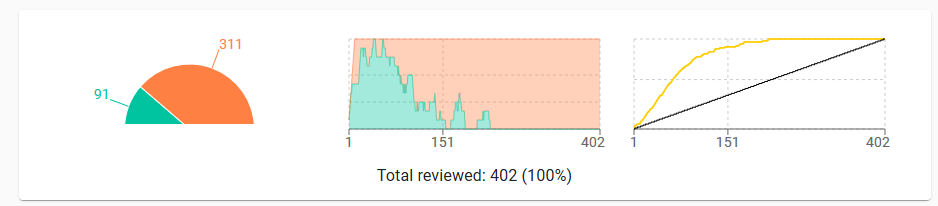
\includegraphics{asreview/capture_final2.png}
\caption{Caption for the picture.}
\end{figure}

Select only select articles

\begin{Shaded}
\begin{Highlighting}[]
\NormalTok{data\_asreview \textless{}{-}}\StringTok{ }\KeywordTok{read.xlsx2}\NormalTok{(}\DataTypeTok{file =} \StringTok{"asreview/asreview\_result\_dropout{-}prediction{-}a{-}systematic{-}literature{-}review{-}v3\_FINAL.xlsx"}\NormalTok{,}\DataTypeTok{sheetIndex =} \DecValTok{1}\NormalTok{,)}
\KeywordTok{str}\NormalTok{(data\_asreview)}
\end{Highlighting}
\end{Shaded}

\begin{verbatim}
## 'data.frame':    402 obs. of  13 variables:
##  $ record_id       : chr  "2" "7" "33" "34" ...
##  $ Unnamed..0      : chr  "3" "9" "35" "36" ...
##  $ category        : chr  "INPROCEEDINGS" "INPROCEEDINGS" "ARTICLE" "ARTICLE" ...
##  $ year            : chr  "2015" "2017" "2014" "2019" ...
##  $ title           : chr  "A Case Study for the Churn Prediction in Turksat Internet Service Subscription" "Churn prediction model for effective gym customer retention" "Churn prediction using comprehensible support vector machine: An analytical CRM application" "A big data analytics model for customer churn prediction in the retiree segment" ...
##  $ abstract        : chr  "Churn prediction is a customer relationship process that predicts for customers who are at the brink of transfe"| __truncated__ "In the fitness industry, rolling gym membership contracts allow customers to terminate a contract with little a"| __truncated__ "Support vector machine (SVM) is currently state-of-the-art for classification tasks due to its ability to model"| __truncated__ "Undoubtedly, the change in consumersâ\200\231 choices and expectations, stemming from the emerging technology a"| __truncated__ ...
##  $ doi             : chr  "10.1145/2808797.2808821" "10.1109/BESC.2017.8256385" "https://doi.org/10.1016/j.asoc.2014.01.031" "https://doi.org/10.1016/j.ijinfomgt.2018.10.005" ...
##  $ journal         : chr  "" "" "Applied Soft Computing" "International Journal of Information Management" ...
##  $ bibtexkey       : chr  "10.1145/2808797.2808821" "8256385" "FARQUAD201431" "SHIRAZI2019238" ...
##  $ author          : chr  "G\\\"ok, Mehmet, \\\"Ozyer, Tansel, Jida, Jamal" "J, Semrl, A, Matei" "M.A.H. Farquad, Vadlamani Ravi, S. Bapi Raju" "Farid Shirazi, Mahbobeh Mohammadi" ...
##  $ source          : chr  "ACM" "IEEE" "SCIENCE" "SCIENCE" ...
##  $ final_included  : chr  "1" "1" "1" "1" ...
##  $ asreview_ranking: chr  "1" "2" "3" "4" ...
\end{verbatim}

\begin{Shaded}
\begin{Highlighting}[]
\NormalTok{data\_asreview \textless{}{-}}\StringTok{ }\NormalTok{data\_asreview[data\_asreview}\OperatorTok{$}\NormalTok{final\_included}\OperatorTok{==}\DecValTok{1}\NormalTok{,]}

\KeywordTok{str}\NormalTok{(data\_asreview)}
\end{Highlighting}
\end{Shaded}

\begin{verbatim}
## 'data.frame':    91 obs. of  13 variables:
##  $ record_id       : chr  "2" "7" "33" "34" ...
##  $ Unnamed..0      : chr  "3" "9" "35" "36" ...
##  $ category        : chr  "INPROCEEDINGS" "INPROCEEDINGS" "ARTICLE" "ARTICLE" ...
##  $ year            : chr  "2015" "2017" "2014" "2019" ...
##  $ title           : chr  "A Case Study for the Churn Prediction in Turksat Internet Service Subscription" "Churn prediction model for effective gym customer retention" "Churn prediction using comprehensible support vector machine: An analytical CRM application" "A big data analytics model for customer churn prediction in the retiree segment" ...
##  $ abstract        : chr  "Churn prediction is a customer relationship process that predicts for customers who are at the brink of transfe"| __truncated__ "In the fitness industry, rolling gym membership contracts allow customers to terminate a contract with little a"| __truncated__ "Support vector machine (SVM) is currently state-of-the-art for classification tasks due to its ability to model"| __truncated__ "Undoubtedly, the change in consumersâ\200\231 choices and expectations, stemming from the emerging technology a"| __truncated__ ...
##  $ doi             : chr  "10.1145/2808797.2808821" "10.1109/BESC.2017.8256385" "https://doi.org/10.1016/j.asoc.2014.01.031" "https://doi.org/10.1016/j.ijinfomgt.2018.10.005" ...
##  $ journal         : chr  "" "" "Applied Soft Computing" "International Journal of Information Management" ...
##  $ bibtexkey       : chr  "10.1145/2808797.2808821" "8256385" "FARQUAD201431" "SHIRAZI2019238" ...
##  $ author          : chr  "G\\\"ok, Mehmet, \\\"Ozyer, Tansel, Jida, Jamal" "J, Semrl, A, Matei" "M.A.H. Farquad, Vadlamani Ravi, S. Bapi Raju" "Farid Shirazi, Mahbobeh Mohammadi" ...
##  $ source          : chr  "ACM" "IEEE" "SCIENCE" "SCIENCE" ...
##  $ final_included  : chr  "1" "1" "1" "1" ...
##  $ asreview_ranking: chr  "1" "2" "3" "4" ...
\end{verbatim}

\hypertarget{copy-dois-to-clipboard-to-import-to-zotero}{%
\section{Copy DOIs to clipboard to import to
Zotero}\label{copy-dois-to-clipboard-to-import-to-zotero}}

\begin{Shaded}
\begin{Highlighting}[]
\NormalTok{text\textless{}{-}}\KeywordTok{as.character}\NormalTok{(data\_asreview}\OperatorTok{$}\NormalTok{doi)}
\NormalTok{text}
\end{Highlighting}
\end{Shaded}

\begin{verbatim}
##  [1] "10.1145/2808797.2808821"                         
##  [2] "10.1109/BESC.2017.8256385"                       
##  [3] "https://doi.org/10.1016/j.asoc.2014.01.031"      
##  [4] "https://doi.org/10.1016/j.ijinfomgt.2018.10.005" 
##  [5] "https://doi.org/10.1016/S1874-8651(09)60003-X"   
##  [6] "https://doi.org/10.1016/j.eswa.2008.07.072"      
##  [7] "https://doi.org/10.1016/j.intmar.2010.04.002"    
##  [8] "https://doi.org/10.1016/j.dss.2016.11.007"       
##  [9] "https://doi.org/10.1016/j.eswa.2011.04.007"      
## [10] "https://doi.org/10.1016/j.asoc.2014.08.041"      
## [11] "https://doi.org/10.1016/j.ejor.2019.03.037"      
## [12] "https://doi.org/10.1016/j.neucom.2016.12.009"    
## [13] "https://doi.org/10.1016/j.ins.2019.12.075"       
## [14] "https://doi.org/10.1016/j.jretconser.2019.101918"
## [15] "https://doi.org/10.1016/j.eswa.2005.09.080"      
## [16] "https://doi.org/10.1016/j.dss.2011.01.002"       
## [17] "10.1016/j.eswa.2020.113779"                      
## [18] "10.1109/ICIEA49774.2020.9102099"                 
## [19] "10.1007/s10115-019-01394-7"                      
## [20] "10.1080/01605682.2020.1776166"                   
## [21] "10.1007/s10586-017-1172-1"                       
## [22] "10.1109/ICECCE47252.2019.8940667"                
## [23] "10.1140/epjds/s13688-018-0165-5"                 
## [24] "10.1109/ICSCEE.2018.8538420"                     
## [25] "10.1109/ICATCCT.2017.8389139"                    
## [26] "10.1016/j.ejor.2017.12.015"                      
## [27] "10.1089/big.2018.0015"                           
## [28] "10.1509/jmr.16.0163"                             
## [29] "10.1057/s41274-016-0176-1"                       
## [30] "10.1007/978-981-10-8228-3_6"                     
## [31] "10.1109/DSAA.2017.42"                            
## [32] "10.1007/s10115-016-0995-z"                       
## [33] "10.1108/JSIT-10-2016-0061"                       
## [34] "10.1109/DSAA.2016.84"                            
## [35] "10.1109/CICN.2015.123"                           
## [36] "10.1109/ICDIM.2016.7829775"                      
## [37] "10.1007/s10115-013-0722-y"                       
## [38] "10.1016/j.dss.2015.02.007"                       
## [39] "10.1016/j.eswa.2014.06.018"                      
## [40] "10.1111/deci.12057"                              
## [41] "10.3233/IDA-130625"                              
## [42] "10.1109/ISTMET.2014.6936498"                     
## [43] "10.4028/www.scientific.net/AMR.989-994.1517"     
## [44] "10.1016/j.procs.2014.05.286"                     
## [45] "10.1016/j.asoc.2013.09.017"                      
## [46] "10.1007/978-3-642-41398-8_31"                    
## [47] "10.1016/j.jbusres.2012.12.008"                   
## [48] "10.1016/j.eswa.2012.07.006"                      
## [49] "10.1016/j.eswa.2012.04.016"                      
## [50] "10.1016/j.eswa.2012.01.014"                      
## [51] "10.1016/j.ejor.2011.09.031"                      
## [52] "10.1504/IJECRM.2012.046470"                      
## [53] "10.1016/j.knosys.2011.12.005"                    
## [54] "10.1016/j.eswa.2011.09.059"                      
## [55] "10.1007/978-3-642-30864-2_21"                    
## [56] "10.1109/ICM.2011.397"                            
## [57] "10.1016/j.eswa.2011.06.028"                      
## [58] "10.1016/j.eswa.2010.08.023"                      
## [59] "10.1504/IJNVO.2011.037162"                       
## [60] "10.1007/978-3-642-15387-7_50"                    
## [61] "10.1016/j.eswa.2009.06.076"                      
## [62] "10.1016/j.eswa.2009.07.029"                      
## [63] "10.1007/978-3-642-10646-0_47"                    
## [64] "10.1016/j.ejor.2008.06.027"                      
## [65] "10.1016/j.eswa.2008.06.121"                      
## [66] "10.1016/j.eswa.2008.07.021"                      
## [67] "10.1016/j.eswa.2008.05.027"                      
## [68] "10.1109/ICNC.2008.724"                           
## [69] "10.1016/j.eswa.2007.07.036"                      
## [70] "10.1016/j.eswa.2006.09.038"                      
## [71] "10.1016/j.eswa.2005.11.037"                      
## [72] "10.1109/TEVC.2003.819264"                        
## [73] "10.1016/S0957-4174(02)00030-1"                   
## [74] "10.1007/978-981-13-1280-9_25"                    
## [75] "10.1007/978-3-642-30864-2_21"                    
## [76] "10.1007/978-3-319-24184-5_35"                    
## [77] "10.1007/s00521-018-3548-4"                       
## [78] "10.1007/978-3-642-13025-0_7"                     
## [79] "10.1007/978-3-642-03730-6_19"                    
## [80] "10.1007/s11235-017-0310-7"                       
## [81] "10.1007/978-3-642-18129-0_41"                    
## [82] "10.1007/978-3-642-35527-1_31"                    
## [83] "10.1007/978-3-642-41398-8_31"                    
## [84] "10.1007/978-3-642-17569-5_30"                    
## [85] "10.1007/s00521-020-04850-6"                      
## [86] "10.1007/978-3-319-13332-4_12"                    
## [87] "10.1007/s10489-013-0440-x"                       
## [88] "10.1057/jt.2010.3"                               
## [89] "10.1186/s40537-019-0264-6"                       
## [90] "10.1007/978-3-319-10774-5_8"                     
## [91] "10.1109/BESC.2017.8256385"
\end{verbatim}

\begin{Shaded}
\begin{Highlighting}[]
\KeywordTok{writeClipboard}\NormalTok{(text)}

\KeywordTok{length}\NormalTok{(text)}
\end{Highlighting}
\end{Shaded}

\begin{verbatim}
## [1] 91
\end{verbatim}

\hypertarget{final-list-91-records}{%
\section{Final list 91 records}\label{final-list-91-records}}

\begin{Shaded}
\begin{Highlighting}[]
\NormalTok{data\_asreview }\OperatorTok{\%\textgreater{}\%}\StringTok{ }\KeywordTok{select}\NormalTok{(title,doi) }\OperatorTok{\%\textgreater{}\%}\StringTok{ }\KeywordTok{distinct}\NormalTok{(title,}\DataTypeTok{.keep\_all =} \OtherTok{TRUE}\NormalTok{) }\OperatorTok{\%\textgreater{}\%}\StringTok{ }\KeywordTok{arrange}\NormalTok{(title)}
\end{Highlighting}
\end{Shaded}

\begin{verbatim}
##                                                                                                                                                           title
## 1                                                                               A big data analytics model for customer churn prediction in the retiree segment
## 2                                                                                                     A Case of Churn Prediction in Telecommunications Industry
## 3                                                                                A Case Study for the Churn Prediction in Turksat Internet Service Subscription
## 4                                                                             A churn prediction model for prepaid customers in telecom using fuzzy classifiers
## 5                           A comparative analysis of data preparation algorithms for customer churn prediction: A case study in the telecommunication industry
## 6                                                                                                              A fuzzy prediction model for calling communities
## 7                                                                                              A Graph-Based Churn Prediction Model for Mobile Telecom Networks
## 8                                                                              A novel evolutionary data mining algorithm with applications to churn prediction
## 9                  An efficient system for customer churn prediction through particle swarm optimization based feature selection model with simulated annealing
## 10                                                                 An empirical evaluation of rotation-based ensemble classifiers for customer churn prediction
## 11                                                                    An innovative optimized model to anticipate clients about immigration in telecom industry
## 12                                                   Analytical CRM in banking and finance using SVM: A modified active learning-based rule extraction approach
## 13                                                                                Applicability of machine-learning techniques in predicting customer defection
## 14                                            Application of Computational Intelligence to Predict Churn and Non-Churn of Customers in Indian Telecommunication
## 15                                                                   Applying CHAID for logistic regression diagnostics and classification accuracy improvement
## 16                                                                                                             Applying data mining to telecom churn management
## 17                                                                                                       Applying Fuzzy Data Mining to Telecom Churn Management
## 18                  Bayesian Network Approach to Predict Mobile Churn Motivations: Emphasis on General Bayesian Network, Markov Blanket, and What-If Simulation
## 19                                                                                                         Behavioral attributes and financial churn prediction
## 20                                                                                  Benchmarking sampling techniques for imbalance learning in churn prediction
## 21                                                             Building comprehensible customer churn prediction models with advanced rule induction techniques
## 22                                                                            Calling communities analysis and identification using machine learning techniques
## 23                                                                            Churn and non-churn of customers in banking sector using extreme learning machine
## 24                                                                                                                     Churn perdiction in the telecom business
## 25                                                                                             Churn Prediction in Banking System using K-Means, LOF, and CBLOF
## 26                                                              Churn prediction in mobile social games: Towards a complete assessment using survival ensembles
## 27                      Churn prediction in subscription services: An application of support vector machines while comparing two parameter-selection techniques
## 28                                                                                                  Churn prediction model for effective gym customer retention
## 29                                                                                                  Churn Prediction Model for Effective Gym Customer Retention
## 30                                                                  Churn prediction using comprehensible support vector machine: An analytical CRM application
## 31                                    Comparison of supervised machine learning techniques for customer churn prediction based on analysis of customer behavior
## 32                                                                               Construction of Bayesian classifiers with GA for predicting customer retention
## 33                                                                                       Credit card churn forecasting by logistic regression and decision tree
## 34                                CRM at a pay-TV company: Using analytical models to reduce customer attrition by targeted marketing for subscription services
## 35                                                                                Customer Churn Models: A Comparison of Probability and Data Mining Approaches
## 36                                        Customer Churn Prediction for a Software-as-a-Service Inventory Management Software Company: A Case Study in Thailand
## 37                                                                                                    Customer Churn Prediction for Broadband Internet Services
## 38                                                        Customer churn prediction in the online gambling industry: The beneficial effect of ensemble learning
## 39                                                                         Customer churn prediction in the telecommunication sector using a rough set approach
## 40                                                               Customer Churn Prediction Modelling Based on Behavioural Patterns Analysis using Deep Learning
## 41                                                                                             Customer churn prediction using improved balanced random forests
## 42                                                                                        Customer event history for churn prediction: How long is long enough?
## 43                                                          Data mining using rules extracted from SVM: An application to churn prediction in bank credit cards
## 44                                               Development of a Bayesian Belief Network-based DSS for predicting and understanding freshmen student attrition
## 45                                                                                                    Dynamic behavior based churn prediction in mobile telecom
## 46                                                   Dynamic churn prediction framework with more effective use of rare event data: The case of private banking
## 47                                                             Dynamic classifier ensemble model for customer classification with imbalanced class distribution
## 48                                                                                      Ensembles of Probability Estimation Trees for Customer Churn Prediction
## 49                                                                                                              Estimating customer churn under competing risks
## 50                                       Estimating the effect of word of mouth on churn and cross-buying in the mobile phone market with Markov logic networks
## 51                                                                        Feature-selection-based dynamic transfer ensemble model for customer churn prediction
## 52                                                                                                 Forecasting client retention â\200” A machine-learning approach
## 53                                Fuzzy Clustering with Ensemble Classification Techniques to Improve the Customer Churn Prediction in Telecommunication Sector
## 54                                                                                                        Handling class imbalance in customer churn prediction
## 55 Hybrid PPFCM-ANN model: an efficient system for customer churn prediction through probabilistic possibilistic fuzzy clustering and artificial neural network
## 56                                                                         Improved churn prediction in telecommunication industry using data mining techniques
## 57                                                  Improved marketing decision making in a customer churn prediction context using generalized additive models
## 58                   Improving customer attrition prediction by integrating emotions from client/company interaction emails and evaluating multiple classifiers
## 59                                                                Improving customer churn prediction by data augmentation using pictorial stimulus-choice data
## 60                                                                Improving Customer Churn Prediction by Data Augmentation Using Pictorial Stimulus-Choice Data
## 61                                                                         Improving customer retention in financial services using kinship network information
## 62                                            Including high-cardinality attributes in predictive models: A case study in churn prediction in the energy sector
## 63                                         Intelligent churn prediction in telecom: employing mRMR feature selection and RotBoost based ensemble classification
## 64                                                                                Intelligent data analysis approaches to churn as a business problem: a survey
## 65                                                                                            Micro- and macro-level churn analysis of large-scale mobile games
## 66                                                                                                 Model of Customer Churn Prediction on Support Vector Machine
## 67                                                                                                                 Modeling churn using customer lifetime value
## 68                                                     New insights into churn prediction in the telecommunication sector: A profit driven data mining approach
## 69                                                                          On the operational efficiency of different feature types for telco Churn prediction
## 70                                                       Optimum profit-driven churn decision making: innovative artificial neural networks in telecom industry
## 71                                                                                                    Predicting customer churn through interpersonal influence
## 72                                                                                      Prediction of customer attrition of commercial banks based on SVM model
## 73                                                                                                Preventing churn in telecommunications: The forgotten network
## 74                                                                                                Preventing Churn in Telecommunications: The Forgotten Network
## 75                                                                Profit-Based Model Selection for Customer Retention Using Individual Customer Lifetime Values
## 76                                                                                Profit optimizing customer churn prediction with Bayesian network classifiers
## 77                       Reconciling performance and interpretability in customer churn prediction using ensemble learning based on generalized additive models
## 78                                                                                               Research on customers churn prediction model based on logistic
## 79                                                                                       Retention futility: Targeting high-risk customers might be ineffective
## 80                                             Rule extraction from support vector machine using modified active learning based approach: An application to CRM
## 81                                                                                           Scalable RFM-Enriched representation learning for churn prediction
## 82                  Separating financial from commercial customer churn: A modeling step towards resolving the conflict between the sales and credit department
## 83                                                                                                        Social network analysis for customer churn prediction
## 84                                                                                                                      Social network analysis in Telecom data
## 85                                                                                                                     Staying Power of Churn Prediction Models
## 86                                                                                      The importance of social embeddedness: Churn models at mobile providers
## 87                                                                     Transfer ensemble model for customer churn prediction with imbalanced class distribution
## 88                                                                          Turning telecommunications call details to churn prediction: A data mining approach
## 89                                             Utilizing Customersâ\200\231 Purchase and Contract Renewal Details to Predict Defection in the Cloud Software Industry
## 90                                                                Variable selection by association rules for customer churn prediction of multimedia on demand
## 91                                                                                  Why you should stop predicting customer churn and start using uplift models
##                                                 doi
## 1   https://doi.org/10.1016/j.ijinfomgt.2018.10.005
## 2                       10.1007/978-3-319-10774-5_8
## 3                           10.1145/2808797.2808821
## 4                         10.1007/s11235-017-0310-7
## 5         https://doi.org/10.1016/j.dss.2016.11.007
## 6                         10.1504/IJNVO.2011.037162
## 7                      10.1007/978-3-642-35527-1_31
## 8                          10.1109/TEVC.2003.819264
## 9                         10.1007/s10586-017-1172-1
## 10       https://doi.org/10.1016/j.eswa.2011.04.007
## 11                     10.1109/ICATCCT.2017.8389139
## 12                       10.1504/IJECRM.2012.046470
## 13                      10.1109/ISTMET.2014.6936498
## 14                            10.1109/CICN.2015.123
## 15                                10.1057/jt.2010.3
## 16       https://doi.org/10.1016/j.eswa.2005.09.080
## 17                     10.1007/978-3-642-18129-0_41
## 18                     10.1007/978-3-642-17569-5_30
## 19                  10.1140/epjds/s13688-018-0165-5
## 20                        10.1057/s41274-016-0176-1
## 21                       10.1016/j.eswa.2010.08.023
## 22       https://doi.org/10.1016/j.eswa.2008.07.072
## 23                      10.1007/978-981-10-8228-3_6
## 24                       10.1109/ICDIM.2016.7829775
## 25                 10.1109/ICECCE47252.2019.8940667
## 26                             10.1109/DSAA.2016.84
## 27                       10.1016/j.eswa.2006.09.038
## 28                        10.1109/BESC.2017.8256385
## 29                        10.1109/BESC.2017.8256385
## 30       https://doi.org/10.1016/j.asoc.2014.01.031
## 31                        10.1108/JSIT-10-2016-0061
## 32                            10.1109/ICNC.2008.724
## 33                       10.1016/j.eswa.2011.06.028
## 34                       10.1016/j.eswa.2005.11.037
## 35                     10.1007/978-3-319-24184-5_35
## 36                  10.1109/ICIEA49774.2020.9102099
## 37                     10.1007/978-3-642-03730-6_19
## 38                    10.1016/j.jbusres.2012.12.008
## 39     https://doi.org/10.1016/j.neucom.2016.12.009
## 40                      10.1109/ICSCEE.2018.8538420
## 41                       10.1016/j.eswa.2008.06.121
## 42                       10.1016/j.eswa.2012.07.006
## 43                     10.1007/978-3-642-10646-0_47
## 44       https://doi.org/10.1016/j.ejor.2019.03.037
## 45                       10.1016/j.eswa.2020.113779
## 46                       10.1016/j.eswa.2014.06.018
## 47                       10.1016/j.eswa.2011.09.059
## 48                      10.1007/978-3-642-13025-0_7
## 49                    10.1080/01605682.2020.1776166
## 50        https://doi.org/10.1016/j.dss.2011.01.002
## 51                        10.1007/s10115-013-0722-y
## 52 https://doi.org/10.1016/j.jretconser.2019.101918
## 53                     10.1007/978-981-13-1280-9_25
## 54                       10.1016/j.eswa.2008.05.027
## 55                        10.1007/s00521-018-3548-4
## 56       https://doi.org/10.1016/j.asoc.2014.08.041
## 57                       10.1016/j.eswa.2009.07.029
## 58                       10.1016/j.eswa.2008.07.021
## 59                     10.1007/978-3-642-30864-2_21
## 60                     10.1007/978-3-642-30864-2_21
## 61                       10.1016/j.eswa.2012.04.016
## 62                        10.1016/j.dss.2015.02.007
## 63                        10.1007/s10489-013-0440-x
## 64                        10.1007/s10115-016-0995-z
## 65                       10.1007/s10115-019-01394-7
## 66    https://doi.org/10.1016/S1874-8651(09)60003-X
## 67                       10.1016/j.ejor.2008.06.027
## 68                       10.1016/j.ejor.2011.09.031
## 69                       10.1016/j.ejor.2017.12.015
## 70                       10.1007/s00521-020-04850-6
## 71                     10.1016/j.knosys.2011.12.005
## 72                      10.1016/j.procs.2014.05.286
## 73                     10.1007/978-3-642-41398-8_31
## 74                     10.1007/978-3-642-41398-8_31
## 75                            10.1089/big.2018.0015
## 76                               10.3233/IDA-130625
## 77                       10.1016/j.eswa.2012.01.014
## 78      10.4028/www.scientific.net/AMR.989-994.1517
## 79                              10.1509/jmr.16.0163
## 80                     10.1007/978-3-642-15387-7_50
## 81                             10.1109/DSAA.2017.42
## 82                       10.1016/j.eswa.2007.07.036
## 83                       10.1016/j.asoc.2013.09.017
## 84                        10.1186/s40537-019-0264-6
## 85     https://doi.org/10.1016/j.intmar.2010.04.002
## 86                               10.1111/deci.12057
## 87                             10.1109/ICM.2011.397
## 88                    10.1016/S0957-4174(02)00030-1
## 89                     10.1007/978-3-319-13332-4_12
## 90                       10.1016/j.eswa.2009.06.076
## 91        https://doi.org/10.1016/j.ins.2019.12.075
\end{verbatim}

\hypertarget{merge-asreview-selected-articles-with-existing-data-for-final-analysis}{%
\section{Merge ASReview selected articles with existing data for final
analysis}\label{merge-asreview-selected-articles-with-existing-data-for-final-analysis}}

\end{document}
